\documentclass[a4paper,UTF8,fontset=windows,AutoFakeBold]{ctexart}
\pagestyle{headings}
\title{\textbf{高等数学A\ 习题课讲义}}
\author{原生生物}
\date{}
\setcounter{tocdepth}{3}
\usepackage{amsmath,amssymb,amsthm,enumerate,framed,geometry,hyperref,paralist,pgfplots,ulem}

\geometry{left = 2.0cm, right = 2.0cm, top = 2.0cm, bottom = 2.0cm}
\ctexset{section={number=\zhnum{section}}}
\ctexset{subsection={name={\S},number=\arabic{section}.\arabic{subsection}}}

\newcommand*{\dr}{\hspace{0.07em}\mathrm{d}}
\newcommand*{\cm}{\mathcal{C}}
\newcommand*{\er}{\mathrm{e}}
\newcommand*{\ir}{\mathrm{i}}
\newcommand*{\nm}{\mathcal{N}}
\newcommand*{\rb}{\mathbb{R}}

\newcommand*{\bm}{\boldsymbol}

\newcommand*{\extra}{\textbf{附加}}

\newcommand*{\note}{\noindent *}

\newtheoremstyle{ex}% name
{3pt}% Space above
{3pt}% Space below
{\songti}% Body font
{}% Indent amount
{\bfseries}% Theorem head font
{.}% Punctuation after theorem head
{.5em}% Space after theorem head
{}% Theorem head spec (can be left empty, meaning ‘normal’)

\theoremstyle{ex}
\newtheorem{exercise}{题}
\newcommand{\exref}[1]{\textbf{题\;\ref{#1}\;}}

\newcommand{\sol}[1]{{\vspace{5pt}\kaishu\noindent\textbf{解答}:\vspace{-3pt}
\begin{compactitem}
    \item[] #1
\end{compactitem}
}}

\pgfplotsset{compat=1.18}

\begin{document}

\maketitle

\note 高等数学A [刘培东老师班]习题课讲义。

\note 由于高等数学是一个需要大量练习的学科,因此习题课的主要组织结构将会是通过\textbf{题目}进行,根据每道题的编号,大家可以看到一学期的知识究竟需要多少个练习来掌握。题目的解答将以{\kaishu\textbf{楷书}}展示,对一些相对复杂的定理,如果时间不够可仅了解结论,跳过证明细节。

\note 讲义中提到的$n$默认为正整数,$n$趋于无穷时的极限均指\textbf{数列极限}。$C_m^n$代表组合数$\frac{m!}{n!(m-n)!}$,且当$m<n$时定义为0。

\tableofcontents

\newpage
\section{难易}
本次习题课主要介绍了大学数学(主要针对高等数学A与线性代数A)相关的学习建议,不存在需要掌握的知识性内容,但仍然\textbf{非常推荐大家阅读}。

\subsection{有关大学数学}
说到关于大学数学的建议,自然需要先从大学数学课与中学阶段数学的本质不同讲起。我们主要分为四件事讨论:文本的重要性、抽象层级的提升、证明逻辑的强化与学习方法的差异。

\subsubsection{文本}
个人一直的观点是,比起课堂,\textbf{对文本的阅读}(尤其是教材)往往是更加重要的。原因有二:一方面,大学数学的内容量大,导致上课需要快速过掉较多内容,这就导致老师的\textbf{节奏}注定只能适合一小部分人,对剩下的同学来说跟上思路是很难的(更大的问题是``老师以为大家会''的东西可能是自己尚未学过的,这种默认知识背景不同的情况会导致更多问题);另一方面,即使能够跟上,上课来不及理解更多细节也会导致\textbf{以为自己懂了},也就是虽然听着感觉理解了,但还是无法做出对应的题目。

——当然,上面说的这两方面问题读文本也会有,但以读为主的的最大好处是,\textbf{按自己节奏阅读的成本很低}。上课时无法随时暂停、快进或重放内容,即使有了录课,如此看一段视频所花的时间也远比读一段教材要高。

接下来,我们该聊聊阅读教材的注意事项了。很显然(这是本讲义第一次出现显然这个词,也将是最后一次),\textbf{朗读}一遍教材是无法对学习有任何帮助的。为了让\textbf{阅读}有超出朗读的效果,有两件事必须注意。首先,一定要注意教材的\textbf{逻辑细节},简单来说,必须知道每个证明里上一句话到下一句话是用了何种\textbf{结论}。教材上的证明往往不会太过困难,这一部分往往是可以通过自己思考解决的。其次,需要掌握教材的\textbf{思路}。小到证明的一步为什么能想到、一个定义为何要出现,大到教材为何如此编排,某章的核心内容是什么,都是\textbf{必须}有自己答案的——稍后我们会解释如此要求的理由。不过,思路相关的问题就很难通过个人思考得到了,甚至每个人的答案都可能不同。因此,遇到这些问题时最好通过\textbf{交流}进行解决,也就是积极去问同学/助教``这个东西是如何想到的'',并在得到的答案中找到自己可以接受的解释,以此进行更深入的理解。

理论上来说,大学的所有课程都可以只通过文本资料学习,无需上课。不过,如果能跟上老师的思路,上课也确实可以收获一些阅读无法收获的东西,我们将在下面继续讨论。

\subsubsection{抽象}
大家学习数学的过程中实际上经历了两次抽象:小学时从两个苹果和三个苹果放在一起是五个苹果到$2+3=5$,是\textbf{具体事物到数字}的抽象;中学时从$(3+2)^2=2^2+2\times2\times3+3^2$到$(a+b)^2=a^2+2ab+b^2$,是\textbf{从数字到符号}(也就是\textbf{代数})的抽象。

在大学,我们将经历第三次抽象(也往往是非数学专业会触及的最后一次抽象):\textbf{从符号到结构}。例如,对于\textbf{加法}(不妨考虑对任何实数的加法),我们可以提取出它的四个核心特征(这里的$\exists!$表示\textbf{存在唯一}):
$$a+b=b+a$$
$$(a+b)+c=a+(b+c)$$
$$\forall a\in\rb,\quad 0+a=a$$
$$\forall a\in\rb,\quad\exists!b\in\rb,\quad a+b=0$$
前两个行称为\textbf{交换律}与\textbf{结合律},第三行代表\textbf{零的存在性},第四个行则代表\textbf{相反数的存在性}。

反过来说,\textbf{只要满足这四个特征的运算就可以称为``加法''}。例如,考虑$\rb^*$,即所有非零实数,它们的乘法满足(第四行即为\textbf{倒数},任何非零实数都有非零的倒数)
$$ab=ba$$
$$(ab)c=a(bc)$$
$$\forall a\in\rb^+,\quad 1a=a$$
$$\forall a\in\rb^*,\quad\exists!b\in\rb^*,\quad ab=1$$
由此,非零实数的乘法也可以看作某种意义上的``加法''。

当然,此时的``加法''就不再是一种特定的\textbf{运算}了,而是代表了一种\textbf{结构}。简单来说,对于一个集合$A$,定义$A$上的一种运算$\oplus$\ (也就是给定$A$中两个元素,生成一个新的$A$中元素),若它满足(第四行中的$e$即为第三行中的$e$)
$$\forall a,b\in A,\quad a\oplus b=b\oplus a$$
$$\forall a,b,c\in A,\quad(a\oplus b)\oplus c=a\oplus(b\oplus c)$$
$$\exists! e\in A,\quad\forall a\in A,\quad e\oplus a=a$$
$$\forall a\in A,\quad\exists!b\in A,\quad a\oplus b=e$$
则称这个集合$A$对运算$\oplus$构成一个\textbf{阿贝尔群},第三行中的$e$称为\textbf{零元},第四行中的$b$可以记为$-a$,也即某种``相反数''。用这套语言来说,$\rb$对加法运算构成一个阿贝尔群,$\rb^*$对乘法运算构成一个阿贝尔群。

——阿贝尔群这个名字并不重要,重要的是,我们把一种具体的加法运算抽象为了一个``类似加法的结构''。这样做的好处就像我们之前的每一次抽象一样,只要证明了这种结构的性质,就可以\textbf{应用在所有具有这种结构的情况里}。

例如,只要集合$A$对运算$\oplus$构成一个阿贝尔群,即有
$$-(a\oplus b)=(-a)\oplus(-b)$$

\sol{
    由定义第四个式子可知,只要验证了
    $$(a\oplus b)\oplus((-a)\oplus(-b))=0$$
    利用``相反数''的唯一性即可得到原式成立。利用结合律,上式左侧等于
    $$((a\oplus b)\oplus(-a))\oplus(-b)$$
    再次利用结合律可将其化为
    $$(a\oplus(b\oplus(-a)))\oplus(-b)$$
    利用交换律可知要证
    $$(a\oplus((-a)\oplus b))\oplus(-b)$$
    再次利用结合律得到
    $$((a\oplus(-a))\oplus b)\oplus(-b)$$
    利用``相反数''的定义可知这等于
    $$(e\oplus b)\oplus(-b)$$
    利用零元的定义可知这等于
    $$b\oplus(-b)$$
    最后再利用``相反数''的定义将其化为0,即得证。
}

将上述定理应用在加法上,可以得到对实数$a,b$有
$$-(a+b)=(-a)+(-b)$$
而应用在非零实数乘法上,即得到了对非零实数$a,b$有
$$\frac{1}{ab}=\frac{1}{a}\cdot\frac{1}{b}$$

由此,我们观察了一个非常简单的\textbf{将符号抽象为结构}的例子,且看到了一些好处。不过,就像之前的每一种抽象是困难的,这一层抽象也存在自己的困难,也就是需要\textbf{暂时丢弃已经学会的内容,只保留最基础的性质并通过全新的方式认知}。

\note 事实上,大家以后或许还会接触到第四层,也是目前我们能研究的最高一层抽象,\textbf{将结构抽象为范畴}。例如,阿贝尔群和集合都是一个\textbf{范畴},这样,我们就可以对比不同范畴之间的共性与不同了。

为了理解抽象,一个必须的办法是\textbf{从具体例子入手}。如果没有$\rb$对加法与$\rb^*$对乘法作为例子,下面的阿贝尔群定义将是\textbf{悬空}的。反之,若是只学具体例子,不去了解阿贝尔群的定义,就无法提取出具体例子的\textbf{共性}——而孤立地去学具体例子在大学是不可行的,因为大学数学的内容量真的很\textbf{大}。

笼统来说,所有具体例子、做题技巧整理都可以称为\textbf{低观点},而所有结构性的内容、抽象层面的讨论都可以称为\textbf{高观点}。当然,应对考试必须掌握足够的低观点,而高观点很多则来自课程与自己的思考。高观点是必要的,就像上面所说的抽象层级,它可以做到提取低观点中的共性以\textbf{更好理解、记忆}。

\note 高等数学课程中的结构想法远不如线性代数中多,但类似的寻找共性的思路仍然可以帮助大家理解很多\textbf{定义、定理的由来}。

\subsubsection{证明}
在大学之前,我们所谓的``证明''其实更多时候是``说明'':只要我们知道一个部分是对的,就可以直接跳过对于这部分的具体细节。

然而,在大学,这件事并不成立。这是由于大学中遇到的\textbf{逻辑}将更加复杂,甚至在有的地方反直觉,导致``知道是对的''并不成立,只有一步步\textbf{推导}出来的内容才能确信是对的。

在之后的习题课中,我们将以更严格的方式叙述逻辑,也将进一步解释为何有些``看起来对''的证明是不合理的,而有些``一时看不出理由''的推导其实是正确的。目前阶段,至少希望大家做到的是,在证明中绝大部分的\textbf{三段论}推导中看出其中用到的\textbf{结论},通俗来说也就是\textbf{能说出每一步的理由}。

当然,这件事的做到只能算是``读懂''了一个证明,还远称不上是\textbf{学会}一个证明。与证明逻辑同等重要的是证明的\textbf{思路},也即\textbf{能说出证明是如何想到的}——这事实上与本章开头讨论文本时的要求完全一致。

一个常见的误区是,数学家的``注意力''是凭空产生的,常人无法想到。事实上,绝大部分证明之所以读着让人感觉无法想到,是因为\textbf{写出的过程与真实思路有很大差异}。例如,虽然结构的呈现都是顺序,写证明时可能是一会儿从条件出发一会儿从结论出发研究的,可能是找了很多具体例子后研究共性,也可能是看别的证明时突然有了思路......知道了这些,我门就可以在遇到思路不明确的证明时多进行不同的尝试,或许就能发现想到这些其实是``自然''的——当然,这个过程里还是要再次强调与人的交流,毕竟一个人确实也不可能想清楚全部的思路。

\subsubsection{方法}
最后,我们来聊一聊学习方法的差别。中学数学的常见(至少我亲身经历中常见)的学习模式是:以记忆做题方法为主线,训练一套``什么题用什么方法''的模式,不太注重\textbf{分析与尝试}本身。

上述的做法在内容量不多时,确实可以成为有效的思路,因为通过大量题目的训练能够快速建立起``看到题目就知道该用什么''的\textbf{直觉}。大学数学里,\textbf{建立直觉}也仍然是很重要的部分——事实上前面所说的数学家的``注意力''就是一种直觉——但绝不可能只靠大量做题达成,这是因为大学的内容量已经\textbf{不可能对每个知识点都做充分多的题目},或用我常说的话,``背是一定\textbf{背不完}的''。

那么,用什么方法能在做题不那么多的时候就达成训练直觉的目的呢?如果用最简单的方法概括,答案就是\textbf{多想}、\textbf{多问}。前者意味着该亲自参与的时候一定要亲自参与,例如习题课一般不会直接讲题目解答,尤其是作业题,因为这是必须自己做了才能有用的部分,没有自己的尝试就不可能知道怎洋的直觉是\textbf{有效}的,怎样是无效的;后者则意味着出现问题时需要及时沟通,因为自己想到的书上/答案写得有差别并不意味着就是错误的,说不定只是某一步需要补全,而自己做不出来时,知道这些只能依靠了解\textbf{其他人能否通过此思路走通}。

\subsection{联系}
\subsubsection{结构与动机}
虽然刚才讲了大学数学与之前数学学习不同的四个方面,大家可以发现它们其实存在很鲜明的共性。具体来说,就是对\textbf{高观点}的更加注重。现在,我们可以详细解释何为大学数学中的高观点了。主要包含两部分:\textbf{结构}与\textbf{动机}。

无论是教材还是上课,资料一定是\textbf{顺序}呈现的,一行后接着另一行。但是,这样的顺序往往不是真正的\textbf{思路结构}。就像本次习题课的真实结构是在黑板上画了一张有着诸多连线的图一样,真正的结构往往至少是\textbf{树状}的——以教材为例,很可能每一章是为了解决某个``主要问题'',此问题可以拆分为若干``次要问题'',并可以进行进一步的拆分,直到得到个人可以解决的一个个小点。更多时候,这样的联系并非单向、逐级向下的,就以高数为例,\textbf{微分}之下的各种结论(如微分中值定理)与\textbf{积分}之下的各种结论(如积分中值定理)很多时候会存在一定程度的\textbf{对应},而这样的对应关系会带来更复杂的连接。所有的这些对结构的分析都是掌握知识的重要一环,也可以切实提升\textbf{理解},也即之前说的,不用记忆就培养直觉的方式。

另一个很重要但必须思考的内容就是\textbf{动机},也即不断反问``为何能够想到''。因为数学世界的一切都是由人类创造的(暂且忽略发明与发现的哲学讨论),\textbf{每一个概念的创造必有其原因}。即使很多时候站在初学角度并不能感知到最准确的理由,对动机有自己的理解仍然是重要的。例如,初学导数时,的确可以将导数理解为``为了刻画\textbf{速度}出现的概念'',即使学到之后对这个概念有了更深的体会,也并不意味着用速度看待导数后对更多知识产生的理解是无效的。

当然,无论是结构还是动机都\textbf{不存在唯一的答案}。哪怕是教材的编写者所说出的结构,也并不一定就是教材是真正结构,因为其中还蕴含着编写者的整个知识体系所带来的理解。某种意义上,听课的最大意义就是\textbf{获取老师对高观点的理解},并以此和直接阅读教材、自己思考结合,得到自己的答案。

——至于为何要强调高观点?正是因为这些部分可以超越简单的背诵,达到\textbf{在有限的时间与做题量下训练出直觉}的效果,所以,千万\textbf{不要觉得以应试为目的的学习就无需掌握高观点},除非你能在刷题的同时记下做过的每一道题目是如何处理的。

\subsubsection{问与想}
在之前介绍方法时,我们已经说了``多想''与``多问''是本质性的解决方法,事实上它们就是\textbf{掌握高观点的必要方式},也是大学数学与中学数学学习不同的本质所在。本章的最后,我们就来聊一聊具体如何多想、多问,概括起来其实只有两点:
\begin{itemize}
    \item \textbf{简单的问题不要怕问}。
    
    总会有人因为担心自己的问题过于简单而害怕来交流,但其实简单的问题恰恰是最需要交流的,一方面大家会存在共性(\sout{其实你不会的大家都不会,不要被群聊里活跃的人吓到}),另一方面解答这些问题的时间很短,而自己思考得到答案的时间则过于长了。

    同样,也不要担心自己``连这都问是不是问题太多了''。事实上,在学习的前期,出现大量问题是正常的,只有找不同人交流、解决了前期的问题后,才能搭起初步的框架,之后遇到的问题更少。
    
    此外,一个常见的\textbf{误区}是,既然有了答案就不用和人交流不会做的题了。但事实上,\textbf{答案是无法代替得到答案的过程的},和人交流是为了知道别人从何种角度得到答案,而非机械记忆某套固定的操作方法。所以,尤其是学习前期,比起看答案,更应该将不会做的题拿给大家交流。

    \note 至于问AI,个人并不推荐,因为它有着和看答案一样的问题:学习前期无法区分结果正误,即使是正确的,也无法得知想到证明所需的知识背景。

    \item \textbf{困难的问题不要怕想}。
    
    既然大家都来到了这里,不需要觉得有什么知识是``自己不配学''的。如果要建立完整的体系,一般都需要掌握全部的知识——除了一些\textbf{过于困难的技巧}可以适当放弃(真有这样的情况会在讲义里提及),其他内容都是理应掌握的。

    如果一时觉得怎么学都无法学会,那往往实际上是\textbf{切入思路}的问题。只要能适当调整思路,多去思考\textbf{如何用自己能理解的方式构建体系},并和人交流,一定可以达成\textbf{不用堆时间也能学会}的效果。

    对于真正困难的内容,充分思考一定是有必要的。事实上,数学上的困难往往就意味着大量不符合直觉、无法通过直觉建构的内容,那么也就必须利用思考构建起\textbf{新的直觉}来进行理解——越是困难的东西,越不能指望通过强行记忆去学,因为困难将导致更容易忘却。
\end{itemize}

希望大家能带着这两句话,完成整个本科的数学学习,并至少\textbf{学有所得}。

\newpage
\section{数列极限}
本次习题课主要介绍了数列极限的部分技巧和一些重要的估算,知识基础为数列极限定义、一些基本的数列极限结果(如夹逼定理、保序性、加减乘除极限等)与单调有界数列存在极限。

\subsection{作业解答}
\begin{enumerate}
    \item (1.3节例7)设$a_n$是非负数列,且
    $$\lim_{n\to\infty}a_n=a\ge0$$
    证明
    $$\lim_{n\to\infty}\sqrt{a_n}=\sqrt{a}$$

    \sol{
        分两种情况:
        \begin{itemize}
            \item 若$a>0$,由于根号难以处理,尝试利用分子有理化直接计算可知
            $$\sqrt{a_n}-\sqrt{a}=\frac{a_n-a}{\sqrt{a_n}+\sqrt{a}}$$
            由于$a$为正,分母必然非零。

            直接缩小分母估算可知
            $$|\sqrt{a_n}-\sqrt{a}|=\frac{|a_n-a|}{\sqrt{a_n}+\sqrt{a}}\le\frac{|a_n-a|}{\sqrt{a}}$$
            由此,对任何$\varepsilon>0$,利用$a_n$极限为$a$,由$\sqrt{a}\varepsilon>0$可以取$N$使得$n>N$时
            $$|a_n-a|<\sqrt{a}\varepsilon$$
            此时即得到
            $$|\sqrt{a_n}-\sqrt{a}|<\varepsilon$$
            从而得证。

            \item 若$a=0$,此时也即求证$\sqrt{a_n}$极限为0。对任何$\varepsilon>0$,利用$a_n$极限为0,由$\varepsilon^2>0$可以取$N$使得$n>N$时
            $$|a_n-0|<\varepsilon^2$$
            此时再利用$a_n\ge0$即得到
            $$|\sqrt{a_n}-0|=\sqrt{a_n}<\varepsilon$$
            从而得证。
        \end{itemize}
    }

    \note 虽然解答中直接进行了分类讨论,直接做时往往会先只考虑到$a>0$的情况,在\textbf{检查过程发现严谨性问题时}(即$a=0$时分母可能为0,且$\sqrt{a}\varepsilon=0$,不是符合要求的正数)再补充另一种情况的证明。因此,一定要注意做完以后检查每步是否能实现。

    \note 当然,$\sqrt{a}\varepsilon$与$\varepsilon^2$的构造也是先有下面的估算再回头进行的,这也是经典的\textbf{解答呈现顺序与真实思路相反}。

    \item (1.3节定理4(3))设
    $$\lim_{n\to\infty}a_n=l_1,\quad\lim_{n\to\infty}b_n=l_2$$
    且$l_2\ne0$,证明
    $$\lim_{n\to\infty}\frac{a_n}{b_n}=\frac{l_1}{l_2}$$

    \sol{
        \begin{itemize}
            \item 定理4(2)已经证明了
            $$\lim_{n\to\infty}a_nb_n=\lim_{n\to\infty}a_n\lim_{n\to\infty}b_n$$
            由此只要证明
            $$\lim_{n\to\infty}\frac{1}{b_n}=\frac{1}{l_2}$$
            即有
            $$\lim_{n\to\infty}\frac{a_n}{b_n}=\lim_{n\to\infty}a_n\lim_{n\to\infty}\frac{1}{b_n}=\frac{l_1}{l_2}$$

            \item 为说明$\lim_{n\to\infty}\frac{1}{b_n}=\frac{1}{l_2}$,我们需要先说明左侧\textbf{定义合理},也即$n$充分大时$b_n$\textbf{非零}。
            
            由于$l_2\ne0$,有$\frac{|l_2|}{2}>0$,于是存在$N$使得$n>N$时
            $$|b_n-l_2|<\frac{|l_2|}{2}$$
            此时利用三角不等式得
            $$|b_n|>\frac{|l_2|}{2}$$
            从而可知$n>N$时$b_n\ne0$,可以定义。

            另一方面,直接计算可知
            $$\bigg|\frac{1}{b_n}-\frac{1}{l_2}\bigg|=\frac{|b_n-l_2|}{|b_nl_2|}$$
            可以发现,在刚才得估算下,$n>N$时可以放大得到
            $$\bigg|\frac{1}{b_n}-\frac{1}{l_2}\bigg|<\frac{|b_n-l_2|}{l_2^2/2}$$
            为了进一步控制,对任何$\varepsilon>0$,利用$b_n$极限为$l_2$,由$\frac{l_2^2}{2}>0$存在$N_0$使得$n>N_0$时
            $$|b_n-l_2|<\frac{l_2^2}{2}\varepsilon$$
            从而可知$n>N$且$n>N_0$时
            $$\bigg|\frac{1}{b_n}-\frac{1}{l_2}\bigg|<\frac{|b_n-l_2|}{l_2^2/2}<\varepsilon$$
            也即取$N_1=\max\{N,N_0\}$可符合极限定义,得证。
        \end{itemize}
    }

    \item (习题1.3.4(1))用定义证明
    $$\lim_{n\to\infty}\frac{3n+1}{2n-3}=\frac{3}{2}$$

    \sol{
        直接计算可知
        $$\bigg|\frac{3n+1}{2n-3}-\frac{3}{2}\bigg|=\frac{11}{|4n-6|}$$
        对任何$\varepsilon>0$,直接解不等式可知使上式小于$\varepsilon$只需
        $$n>\frac{1}{4}\bigg(\frac{11}{\varepsilon}+6\bigg)$$
        从而取($[x]$代表不超过$x$的最大整数)
        $$N=\left[\frac{1}{4}\bigg(\frac{11}{\varepsilon}+6\bigg)\right]+1$$
        即符合要求。
    }

    \item (习题1.3.5)设
    $$\lim_{n\to\infty}a_n=0$$
    且数列$b_n$有界,即
    $$\exists M>0,\quad\forall n\in\mathbb{N}^*,\quad|b_n|<M$$
    证明
    $$\lim_{n\to\infty}a_nb_n=0$$

    \sol{
        由条件可知
        $$|a_nb_n|=|b_n||a_n|\le M|a_n|$$
        对任何$\varepsilon>0$,利用$a_n$极限为0,由$\frac{\varepsilon}{M}>0$存在$N$使得$n>N$时
        $$|a_nb_n-0|=|a_nb_n|\le M|a_n|<\varepsilon$$
        从而符合极限定义,得证。
    }

    \note 仍然注意我们一定是\textbf{先进行估算},\textbf{再利用定义取合适的数}。
    
    \item (习题1.3.7)计算极限:
    \begin{enumerate}
        \item[(1)] $$\lim_{n\to\infty}(\sqrt{n+1}-\sqrt{n})$$
        
        \sol{
            利用分子有理化技术可知
            $$|\sqrt{n+1}-\sqrt{n}|=\sqrt{n+1}-\sqrt{n}=\frac{1}{\sqrt{n+1}+\sqrt{n}}<\frac{1}{\sqrt{n}}$$
            由此对任何$\varepsilon>0$,直接解不等式可知使上式小于$\varepsilon$只需
            $$n>\frac{4}{\varepsilon^2}$$
            从而取
            $$N=\bigg[\frac{4}{\varepsilon^2}\bigg]+1$$
            即符合极限定义,得证原式极限为0。
        }

        \item[(3)] $$\lim_{n\to\infty}\frac{(2n+10)^4}{n^4+n^3}$$
        
        \sol{
            分子分母同除以$n^4$可得上式等于
            $$\lim_{n\to\infty}\frac{(2+10/n)^4}{1+1/n}$$
            由于
            $$\lim_{n\to\infty}\frac{1}{n}=0$$
            利用乘积极限、加法极限结论即得
            $$\lim_{n\to\infty}\bigg(1+\frac{1}{n}\bigg)=1,\quad\lim_{n\to\infty}\bigg(2+\frac{10}{n}\bigg)=2$$
            进一步利用乘除法极限结论即得原式为
            $$\frac{2^4}{1}=16$$
        }
    \end{enumerate}
\end{enumerate}

\note 请一定注意书写证明时添加\textbf{必要的文字说明}以表明\textbf{逻辑},可以注意习题解答中\textbf{关联词}的使用。

\subsection{严谨性}
\subsubsection{替换原理}
我们首先需要了解证明过程中最常用的原理之一(由于我们并不关注数理逻辑的细节,本讲义将所有可以用于证明的逻辑理论称为\textbf{原理}):\textbf{替换原理}。

举例来说,假设
$$\lim_{n\to\infty}a_n=a$$
为什么我们可以将极限定义里的$\varepsilon$替换为$\frac{\varepsilon}{2}$呢?事实上分为两步。首先,上式根据定义是(默认$n$、$N$为正整数)
$$\forall\varepsilon>0,\quad\exists N,\quad\forall n>N,\quad|a_n-a|<\varepsilon$$
由于$\varepsilon$本身只是一个形式的记号,我们可以将它作任意的\textbf{替换},例如替换为$\frac{\varepsilon}{2}$,可以得到
$$\forall\frac{\varepsilon}{2}>0,\quad\exists N,\quad\forall n>N,\quad|a_n-a|<\frac{\varepsilon}{2}$$
而另一方面,我们知道一个数除以2是正数与这个数是正数等价,将逻辑上等价的式子进行\textbf{替换}就得到了
$$\forall\varepsilon>0,\quad\exists N,\quad\forall n>N,\quad|a_n-a|<\frac{\varepsilon}{2}$$
也就是说,这个过程里进行了两步,先对形式记号进行了替换,再对逻辑上等价的式子进行替换。每一步替换前后,所得的命题都等价。

但是,至此,我们还需要提问,这两个替换随时都可以进行吗?举例来说,考虑如下的命题
$$\forall x\in\rb,\quad\exists y\in\rb,\quad y>x$$
我们把$x$替换为$2x$或$x^2$不会影响此命题,但如果替换为$x^2+y$,就能得到荒谬的结果:
$$\forall x^2+y\in\rb,\quad\exists y\in\rb,\quad y>x^2+y$$
这意味着,对形式变量的替换似乎确实不是任何时候都可以进行的。最关键的事情是,我们需要保证替换前后变量的\textbf{自由性}不变。也即,替换前的$x$不会受第二个条件$\exists y\in\rb$约束,那么无论替换成$z$或$w$都可以,但一定\textbf{不能与$y$有关}。

本节的``替换原理''实际上是指第一种情况,至于第二种情况,对于等价命题的替换,确实是在任何时候都可以进行的,我们可以称为``等价原理''。更复杂的替换\textbf{不等价命题}的情况我们将在下一节介绍。

讲到这里,就可以纠正不少同学在证明时容易犯的错误了。

\begin{framed}
\begin{exercise}\label{not equal}
    下面的两个命题(称为命题2、命题3)与$a_n$在$n$趋于无穷时极限是$a$\ (称为命题1)等价吗?若不等价,它们的推出关系是怎样?
    $$\forall\varepsilon>0,\quad\exists N,\quad\forall n>N,\quad|a_n-a|<\frac{\varepsilon}{N}$$
    $$\forall\varepsilon>0,\quad\exists N,\quad\forall n>N,\quad|a_n-a|<\frac{\varepsilon}{n}$$
\end{exercise}
\sol{
    首先,命题2与命题3都能推出命题1,这是由于$N$、$n$都是正整数,因此$|a_n-a|<\frac{\varepsilon}{N}$或$|a_n-a|<\frac{\varepsilon}{n}$都意味着$|a_n-a|<\varepsilon$,命题1已经成立(此处的严格逻辑见下一节)。

    此外,命题3也可以推出命题2,这是因为在$n>N$的条件下$|a_n-a|<\frac{\varepsilon}{n}$也可以推出$|a_n-a|<\frac{\varepsilon}{N}$。

    命题1不能推出命题2,考虑数列
    $$a_n=n^{-1/2}$$
    其极限为0,但取$\varepsilon=0.5$,无论如何取$N$都无法保证$n>N$时$\frac{1}{\sqrt{n}}<\frac{1}{2N}$,矛盾。

    \note 此处构造思路为,命题2与命题3接近,而命题3本质是$n|a_n-a|$趋于0,因此$a_n$趋于0且$na_n$不趋于0很可能可以导出矛盾。三个命题里$\varepsilon$、$N$、$n$可以分别取,这就是\textbf{受约束性}带来的。

    命题2不能推出命题3,不过反例相对复杂:记$b_n=na_n$,我们进行如下的构造:
    $$b_1=0,\quad b_2=1$$
    $$b_3=0,\quad b_4=\frac{1}{2}=\frac{3}{6},\quad b_5=\frac{4}{6},\quad\dots,\quad b_7=1$$
    $$b_8=0,\quad b_9=\frac{1}{3}=\frac{8}{24},\quad b_{10}=\frac{9}{24},\quad\dots,\quad b_{25}=1$$
    $$\dots$$
    可以发现,由于$|a_n|\le\frac{1}{n}$,有$a=0$,此时命题3等价于$|b_n|\to0$,结论不成立。对于命题2,对任何在$\frac{1}{k-1}$与$\frac{1}{k}$之间的$\varepsilon$\ ($k$为正整数,若$\varepsilon>1$则取$k=1$),考虑上方构造的第$k$行,令$N$为这行的第一个下标,可以验证此后均成立(事实上下方第一个不等号就是构造的想法来源)
    $$\forall n>N,\quad|b_n|\le\frac{n-1}{kN}<\frac{n}{kN}<\frac{n\varepsilon}{N}$$
    这即得到了$|a_n|<\frac{\varepsilon}{N}$,结论成立。

    \note 上方的证明和构造稍有技巧性,需要对概念较为熟悉以后才能想到。我自己构造此数列也尝试了挺久,一个\textbf{更简单的构造}是,将上述$b_n$不为1的项都改为0,可用完全相同的方式证明成立性。由此可以类似发现,$b_n$只需取0或1,且1相距``足够远''就能得到反例,例如只有当$n=k!$\ ($k$为正整数)时$b_n$为1,其他为0。

    \note \textbf{学会构造反例是重要的},因为反例可以帮助大家判断一个``看起来可能对''的逻辑是不是真的正确。稍后我们将看到更复杂的例子。
}
\end{framed}

\note 事实上,进行了``不合法的替换''并非得到的结论一定错,但从逻辑上来说确实\textbf{无法直接推出}。

\

总之,在进行形式记号的替换时,必须保证\textbf{自由变量替换为自由变量},而\textbf{不能涉及在该命题中受到约束的变量}。当然,不同命题中可能有不同的自由变量,如果在其他地方得到了一个正整数$M$,将$\varepsilon$替换为$\frac{\varepsilon}{M}$也是可行的。

\subsubsection{任意与存在}
接下来,我们将介绍大学中常用而高中几乎不会出现的,关于``任意''与``存在''的几条原理。先来看一个经典的问题``找命题的否定'':

\begin{framed}
\begin{exercise}\label{no}
    给出如下命题的否定:对任意$M>0$,存在正整数$N$使得对任意$n>N$有$|a_n|>M$。
\end{exercise}
\sol{
    至少大家应该或多或少接触过(如果没有接触过就请现在\textbf{记住})一个结论:一个包含任意、存在的命题的否定,只要把\textbf{任意改成存在}、\textbf{存在改成任意},然后\textbf{将最后一句话改为否定即可}。也就是说,上述命题的否定为:

    存在$M>0$使得对任意正整数$N$都存在$n>N$满足$|a_n|\le M$。 
    
    \note 题目中的命题可以写为$\lim_{n\to\infty}a_n=\infty$,本讲义第4章将讨论相关定义。
}
\end{framed}

\note 本部分接下来的内容都\textbf{与考试无关},但如果大家能看完,会更能理解证明中的\textbf{逻辑}。

不知道大家是否想过,为何这样的做法是有道理的呢?这些有关证明、命题的东西就涉及到数学的一个重要且基础的分支,\textbf{数理逻辑}。正如其他数学分支一样,数理逻辑也需要一些公理与定理作为支撑,如上节所说,我们将它们称为\textbf{原理},关于任意与存在,可以有着以下的原理:
$$(\neg\exists xA(x))\leftrightarrow(\forall x\neg A(x))$$
我们简单介绍一下上方的记号:这里的$A(x)$不是函数,而是一个关于$x$的\textbf{命题},数理逻辑中研究的对象几乎都是命题;$\leftrightarrow$表示左右可以互相\textbf{推出},我们用$\leftarrow$或$\to$表示单侧的推出;$\neg$表示对后方命题的\textbf{否定};$\exists xA(x)$表示存在$x$使命题$A(x)$成立,这\textbf{仍然是一个命题},而$\forall xA(x)$则表示对任何$x$,命题$A(x)$都成立——自然,$\forall x\neg A(x)$表示对任何$x$,命题$A(x)$都不成立。

\note 注意此原理也是一个命题,而我们将它称为原理说明这个命题\textbf{恒真},无论$A(x)$是何种命题,上方命题都成立。

由此,我们可以将上方这句话解释为:以下两个命题相互等价:不存在$x$使得命题$A(x)$成立、对任意$x$命题$A(x)$不成立。当然,这句话很符合\textbf{直觉}(至于究竟什么是逻辑直觉,这是哲学家们研究的领域),我们下面将用它推导出\exref{no}的更严谨解答。分为以下步骤:
\begin{enumerate}
    \item 对于\textbf{推出}($\to$)的更严谨理解
    
    所谓的$p\to q$\ (这里的字母默认代表\textbf{命题}),一个符合直觉的定义即,假设$p$成立,可以\textbf{证明}$q$成立——篇幅所限,我们不会讨论数理逻辑中究竟何为一个证明。不过,之所以单独讨论这件事,是因为存在一个必须理解的事情:\textbf{假命题可以推出任何命题}。

    虽然这件事基本可以当作推出定义的一部分,但由于它并不像我们使用的其他原理一样符合直觉,我们必须作一定的说明。一个相对合理的理解是,这其实是为了让\textbf{任意}符合逻辑直觉。

    当我们在说\textbf{任意一个三角形都有三条边}时,我们其实在说,对任意一个图形$G$,$G$是三角形可以\textbf{推出}$G$有三条边。这句话当然是正确的,因此,这句话\textbf{对任意图形都正确}——也就是说,在``$G$不是三角形''时,``$G$是三角形可以推出$G$有三条边''仍然是正确的。

    一件明显的事是,无论右边的命题是不是``$G$有三条边'',我们都不希望``$G$不是三角形''的情况影响整个命题的正确性,出于``任意''的语义,我们必须规定\textbf{$G$不是三角形}时,无论$p$是什么命题,``\textbf{$G$是三角形可以推出$p$}''都是真的,这就是所谓的假命题可以推出任何命题。

    \note 另一种方式是将它理解为关联词\textbf{如果}、\textbf{则},假设``如果''后的内容已经不成立,这句话本身不会被违反。

    \note 事实上,在数理逻辑中,``假设$p$成立可以证明$q$成立''并不是$p\to q$的定义,两者的等价性是一个称为\textbf{演绎定理}的定理。

    \item $(p\rightarrow q)\to(\neg q\rightarrow\neg p)$\textbf{恒真}
    
    我们将用到以下\textbf{双重否定原理}:
    $$\neg\neg p\leftrightarrow p$$
    也即对命题$p$,其双重否定与自身等价。

    现在,我们假设$p\rightarrow q$已经成立,来证明$\neg q\rightarrow\neg p$。为证明$\neg q\rightarrow\neg p$,我们进一步假设$\neg q$成立,此时若$p$成立,利用$p\to q$可知$q$成立。由于$\neg q$成立,``$\neg q$不成立''不成立,也即$\neg\neg q$不成立,利用双重否定原理可知$q$不成立,这就得到了矛盾。

    \note 反证法的原理是对命题$r$,$\neg r$与$r$至少有一个成立,这称为\textbf{排中律}(注意这并没有保证两者恰有一个成立,而我们刚才证明了至多有一个,因此的确恰有一个)。

    \note 将$p$、$q$替换为$\neg q$、$\neg p$,结合双重否定原理将等价部分进行替换即可以得到下式恒真:
    $$(\neg q\rightarrow\neg p)\to(p\rightarrow q)$$
    综合上方即得下式恒真:
    $$(\neg q\rightarrow\neg p)\leftrightarrow(p\rightarrow q)$$
    这就是\textbf{逆否命题与原命题等价}。

    \item $(\neg\forall xA(x))\leftrightarrow(\exists x\neg A(x))$\textbf{恒真}

    我们将已知的原理$(\neg\exists xA(x))\leftrightarrow(\forall x\neg A(x))$拆成
    $$(\neg\exists xA(x))\rightarrow(\forall x\neg A(x))$$
    $$(\forall x\neg A(x))\rightarrow(\neg\exists xA(x))$$
    两块,利用第二部分推导可知可以颠倒方向后两侧同加否定,也即下方两式恒真:
    $$(\neg\forall x\neg A(x))\rightarrow(\neg\neg\exists xA(x))$$
    $$(\neg\neg\exists xA(x))\rightarrow(\neg\forall x\neg A(x))$$
    利用双重否定原理可以替换得到下方两式恒真:
    $$\exists xA(x)\rightarrow(\neg\forall x\neg A(x))$$
    $$(\neg\forall x\neg A(x))\rightarrow\exists xA(x)$$
    将命题$A(x)$利用替换原理替换为$\neg A(x)$,可得下方两式恒真:
    $$\exists x\neg A(x)\rightarrow(\neg\forall x\neg\neg A(x))$$
    $$(\neg\forall x\neg\neg A(x))\rightarrow\exists x\neg A(x)$$
    再次利用双重否定原理可得下方两式恒真:
    $$\exists x\neg A(x)\rightarrow(\neg\forall xA(x))$$
    $$(\neg\forall xA(x))\rightarrow\exists x\neg A(x)$$
    将两个命题合并即为结论。

    \item 对\textbf{任意}与\textbf{存在}的进一步讨论
    
    值得注意的是,在\exref{no}中,我们事实上并没有见到$\forall xA(x)$或$\exists xB(x)$这样形式的命题。与之相对,我们见到的是类似
    $$\forall p(x),A(x),\quad\exists q(x),B(x)$$
    的形式(注意以上两个命题\textbf{并非严谨的数理逻辑写法}),那么,它们是什么含义呢?

    在第一部分推导中,我们已经得到了$\forall p(x),A(x)$的含义事实上是
    $$\forall x,p(x)\to A(x)$$
    也就是说,当我们在说$\forall x>0,x^3>0$时,我们指的其实是,对任何$x$,$x>0$能推出$x^3>0$。

    然而,对于存在,$\exists q(x),B(x)$并不代表$\exists x,q(x)\to B(x)$。我们以$\exists x>0,x^2<0$为例,这当然是一个假命题,但是正如第一部分讨论的\textbf{假命题可以推出任何命题},既然有$x$使得$x>0$为假,$\exists x,(x>0)\to(x^2<0)$应当是一个真命题。
    
    仔细观察可以发现,存在事实上是在说\textbf{且},也即$\exists q(x),B(x)$的真正解释是
    $$\exists x,q(x)\land B(x)$$
    也就是说,当我们再说$\exists x>0,x>1$时,我们指的其实是,有一个$x$使得$x>0$成立、$x>1$也成立。

    \item $\neg(p\land q)\leftrightarrow(p\to\neg q)$\textbf{恒真}
    
    \note 我们默认$\neg$和$\leftrightarrow$同时出现时先计算$\neg$。
    
    先证明$\neg(p\land q)\rightarrow(p\to\neg q)$恒真:只需说明$\neg(p\land q)$成立时,若$p$成立则$\neg q$成立。由于$\neg(p\land q)$成立,$p$与$q$不同时成立,而$p$成立则$q$不成立,利用排中律也即$\neg q$成立。

    再证明$(p\to\neg q)\rightarrow\neg(p\land q)$恒真:若$p$能推出$\neg q$,若$p$为假则$p\land q$不成立,若$p$为真可推出$q$为假,因此$p\land q$也不成立,两者结合即说明$\neg(p\land q)$必然成立。

    综合以上两部分得证。
    
    \item $\neg(p\to q)\leftrightarrow(p\land\neg q)$\textbf{恒真}
    
    将第五部分推导的结论拆分为
    $$\neg(p\land q)\rightarrow(p\to\neg q)$$
    $$(p\to\neg q)\rightarrow\neg(p\land q)$$
    利用第二部分推导并通过双重否定原理进行替换可得以下两式恒真:
    $$\neg(p\to\neg q)\rightarrow(p\land q)$$
    $$(p\land q)\rightarrow\neg(p\to\neg q)$$
    将$q$替换为$\neg q$并通过双重否定原理进行替换可得以下两式恒真:
    $$\neg(p\to q)\rightarrow(p\land \neg q)$$
    $$(p\land \neg q)\rightarrow\neg(p\to q)$$
    
    将两个命题合并即为结论。

    \item 最终推导
    
    我们将\exref{no}形式化地写为
    $$\forall p(M),\exists q(N),\forall r(n,N),s(n,M)$$
    这里$p$、$q$、$r$、$s$均代表命题。

    为了得到其否定,我们先利用第四部分推导将其改写为符合数理逻辑要求的形式
    $$\forall M,p(M)\to(\exists N,q(N)\land(\forall n,r(n,N)\to s(n,M)))$$
    接下来,我们想知道此命题的否定
    $$\neg(\forall M,p(M)\to(\exists N,q(N)\land(\forall n,r(n,N)\to s(n,M))))$$
    的等价表述。

    利用第三部分推导,将$p(M)\to(\exists N,q(N)\land(\forall n,r(n,N)\to s(n,M)))$视为一个命题,可知上式等价于
    $$\exists M,\neg(p(M)\to(\exists N,q(N)\land(\forall n,r(n,N)\to s(n,M))))$$
    利用第六部分推导,将$\exists N,q(N)\land(\forall n,r(n,N)\to s(n,M))$视为一个命题,利用等价替换可知上式等价于
    $$\exists M,p(M)\land\neg(\exists N,q(N)\land(\forall n,r(n,N)\to s(n,M)))$$
    可以发现,此时前面的部分已经符合了第四部分推导中的讨论,从而可以形式化写成
    $$\exists p(M),\neg(\exists N,q(N)\land(\forall n,r(n,N)\to s(n,M)))$$
    进一步利用关于任意与存在的原理可知上式等价为
    $$\exists p(M),\forall N,\neg(q(N)\land(\forall n,r(n,N)\to s(n,M)))$$
    利用第五部分推导可知上式等价为
    $$\exists p(M),\forall N,q(N)\rightarrow\neg(\forall n,r(n,N)\to s(n,M))$$
    再次利用第四部分推导可知上式可以形式化写成
    $$\exists p(M),\forall q(N),\neg(\forall n,r(n,N)\to s(n,M))$$
    再次利用第三部分推导、第六部分推导可知上式等价为
    $$\exists p(M),\forall q(N),\exists n,r(n,N)\land\neg s(n,M)$$
    最后利用第四部分推导形式化写为
    $$\exists p(M),\forall q(N),\exists r(n,N),\neg s(n,M)$$
    可以发现,这恰好是题目中存在改成任意、任意改成存在、将最后一句话改为否定的结果,符合我们之前找到的\textbf{规律}。
\end{enumerate}

事实上,上方的证明并非数理逻辑上严谨的证明,但对于尚未学过数理逻辑的同学们来说已经足以作为对逻辑的\textbf{理解}。所谓大学数学的证明逻辑更加复杂,往往就是这些任意、存在、推出、否定的\textbf{相互嵌套},如果说上述过程能对证明书写有什么启示,大概就是\textbf{分析好每一层的逻辑},并\textbf{逐层进行操作},而不是试图一口气给出全部的逻辑。

\note 例如,本次作业里的1.3节例7中,由于$a_n$极限为$a$是\textbf{条件},相应的极限定义中的$\varepsilon$可以\textbf{任取},而$\sqrt{a_n}$极限为$\sqrt{a}$是\textbf{目标},相应的极限定义中的$\varepsilon$\textbf{需要被任意给定}。因此,我们必须以$|\sqrt{a_n}-\sqrt{a}|<\varepsilon$为目标,通过在$a_n$极限为$a$的定义中\textbf{取出}适当的值(如$a>0$时为$\sqrt{a}\varepsilon$)作为限制。

最后介绍两个上方并未涉及的重要性质:
\begin{enumerate}
    \item 等价具有\textbf{自反性}、\textbf{对称性}与\textbf{传递性}:
    $$p\leftrightarrow p$$
    $$(p\leftrightarrow q)\to(q\leftrightarrow p)$$
    $$((p\leftrightarrow q)\land (q\leftrightarrow r))\to(p\leftrightarrow r)$$
    $\land$这个符号表示\textbf{且},也即左右两个命题都成立。上述三个定理也即:命题$p$与自身等价;对命题$p$、$q$,若$p$、$q$等价则$q$、$p$等价;对命题$p$、$q$、$r$,若$p$、$q$等价且$q$、$r$等价,则$p$、$r$等价。

    \note 大家有兴趣可以用我们已经说的内容自行证明它们,不含存在与任意时的等价原理事实上可以通过类似思路证明。

    \item \textbf{不等价命题}也可以替换:
    $$(p(x)\to q(x))\to(\forall xp(x)\to \forall xq(x))$$
    $$(p(x)\to q(x))\to(\exists xp(x)\to \exists xq(x))$$
    也就是说,只要$p(x)\to q(x)$,无论前面如何套存在与任意,推出性仍然成立,这就说明了\exref{not equal}证明的第一部分是合理的。$p(x)\leftrightarrow q(x)$时的情况只是上述替换的特例。
\end{enumerate}

\subsection{证明的思路}
\subsubsection{存在性问题的非构造证明}
本节我们终于将离开上方的纯抽象逻辑层面推导,回到具体的\textbf{证明技巧}来。希望大家能在学习各种技巧性内容时也注意自身的逻辑为何是合理的。

首先,我们将考虑一类\textbf{存在性}问题:问题的最终形式是说明存在$x$满足某些性质。自然地,最直接的方法是直接找到$x$,这称为\textbf{构造性证明}。构造性证明的技巧有很多,其中最重要的往往是先试着\textbf{感性认知}命题在``说什么'',再从所述的内容中找到符合要求的对象。

\note 例如,通过\textbf{反例构造}说明推导不成立即是一种构造性证明。从逻辑的角度来说,反例构造是为了说明命题$p$不能推出命题$q$,而只要找到命题$p$为真、命题$q$为假的\textbf{例子},即能说明这点。由于我们之后还将见到各种各样的反例,此处不再对构造性证明做更多展开。

不过,存在性问题事实上并非一定要通过构造证明。我们来看一个经典且有趣的例子:
\begin{framed}
\begin{exercise}
    证明存在正无理数$a$、$b$使得$a^b$是有理数。
\end{exercise}
\sol{
    考虑$c=\sqrt{2}^{\sqrt2}$,若$c$是\textbf{有理数},取$a$、$b$均为$\sqrt2$可得命题成立,\textbf{否则},由于
    $$c^{\sqrt2}=\sqrt{2}^{\sqrt2\cdot\sqrt2}=2$$
    取$a=c$、$b=\sqrt2$可得命题成立。
}
\end{framed}
在这个例子中,我们并没有显式构造出结果,但却的确得到了结论,这就是依赖\textbf{排中律}:既然$c$要么是有理数要么是无理数,只要两种情况都能得到结论,就能得到原命题结论成立。

除了这样的讨论外,在高等数学中还有一个常用的构造思路,我们姑且称为\textbf{猎人兔子原理}:猎人在数轴上设立了一个长为$x>0$的坑,则一只步长小于$x$的兔子从左到右跳时一定会落到坑里。我们先用它解决下面的被称为\textbf{有理数稠密性}的问题:
\begin{framed}
\begin{exercise}
    证明对任何$a<b$,存在有理数$x\in(a,b)$。
\end{exercise}
\sol{
    由于$b-a>0$,我们可以取出正整数$n$使得
    $$\frac{1}{n}<b-a$$
    此时通过猎人兔子原理已经可以感受到存在整数$m$使得$\frac{m}{n}\in(a,b)$,下面我们来严谨证明此结论。

    为了说明兔子总有一步将跳进坑里,我们其实只需要证明兔子``走过坑的第一步''一定会落在坑里。也即,我们取$m$为\textbf{满足$m>na$的最小整数$m$}。

    此时,利用最小性可以发现
    $$m-1\le na$$
    将定义与上式两侧同除以$n$得到
    $$\frac{m}{n}>a,\quad\frac{m}{n}-\frac{1}{n}\le a$$
    而第二式即得
    $$\frac{m}{n}\le a+\frac{1}{n}<b$$
    从而令$x=\frac{m}{n}$,由于其为整数除以正整数,必然为有理数,而由已证$x\in(a,b)$,因此符合要求。
}
\end{framed}

\textbf{无理数稠密性}其实也可以类似证明,只是有一处需要注意:
\begin{framed}
\begin{exercise}
    证明对任何$a<b$,存在无理数$x\in(a,b)$。
\end{exercise}
\sol{
    我们先尝试\textbf{模仿之前的证明}:由于$b-a>0$,我们可以取出正整数$n$使得
    $$\frac{\sqrt2}{n}<b-a$$
    通过猎人兔子原理感受后,我们试着严谨证明此结论。

    为了说明兔子总有一步将跳进坑里,我们其实只需要证明兔子``走过坑的第一步''一定会落在坑里。也即,我们取$m$为\textbf{满足$\sqrt{2}m>na$的最小整数$m$}。

    此时,利用最小性可以发现
    $$\sqrt{2}m-\sqrt{2}\le na$$
    将定义与上式两侧同除以$n$得到
    $$\frac{\sqrt{2}m}{n}>a,\quad\frac{\sqrt{2}m}{n}-\frac{\sqrt2}{n}\le a$$
    而第二式即得
    $$\frac{\sqrt2m}{n}\le a+\frac{\sqrt2}{n}<b$$
    但是,在令$x=\frac{\sqrt2m}{n}$时,虽然仍然可以得到$x\in(a,b)$,却会发现一个问题:当$m=0$时,$x=0$是\textbf{有理数}。

    由此,上述取法只能在$0\notin(a,b)$时保证成立,在$0\in(a,b)$时需要寻找其他证明方法。事实上这并不困难:由条件$b>0$,因此存在正整数$n$使得$\frac{\sqrt2}{n}<b$,又由于其大于0,令$x=\frac{\sqrt2}{n}$即得$x\in(0,b)\subset(a,b)$,符合要求。综合这部分与之前的证明即得到结论。

    \note 证明的严谨性\textbf{即使步骤看似简单也需要检查},否则很可能发生意料之外的错误。
}
\end{framed}

在直接利用此原理解决了一些问题后,我们就可以研究下面这个似乎很难找到思路的问题了(注意这仍然是一个存在性问题,因为极限存在的定义开头是$\forall\varepsilon>0$,证明不存在则要说明$\exists\varepsilon>0$):
\begin{framed}
\begin{exercise}\label{sin n}
    证明$\sin n$在$n$趋于无穷时的极限不存在。
\end{exercise}
\sol{
    我们分为三步证明:
    \begin{itemize}
        \item 初步分析
        
        由于$|\sin n|\le 1$恒成立,这是一个\textbf{有界}数列,为了证明其极限不存在,我们可以先尝试\textbf{找}一个有界但极限不存在的数列,如$a_n=(-1)^n$进行观察。

        可以发现,它不存在极限的本质原因是不断在上下振荡。我们试着将它总结为一个\textbf{引理}:若对数列$a_n$,存在$t_1<t_2$使得$a_n$中有无穷多项小于$t_1$、有无穷多项大于$t_2$,则$a_n$不存在极限。

        \note 事实上,若$a_n$有界且极限不存在,一定能找到上述的$t_1$与$t_2$,不过此证明需要的分析技巧较多,不在课程要求内,我们将在证明最后进行补充。
        
        \item 引理证明
        
        若引理不成立,假设$a_n$极限为$l$,则在极限定义中取$\varepsilon=\frac{t_2-t_1}{2}$可得
        $$\exists N,\quad\forall n>N,\quad|a_n-l|<\frac{t_2-t_1}{2}$$
        
        \note 当然,这个取法也是有了下方的估算后才得到的。

        若$l\ge\frac{t_1+t_2}{2}$,上方的式子可以说明第$N$项后所有$a_n$都满足
        $$a_n>l-\frac{t_2-t_1}{2}\ge t_1$$
        与有无穷多项小于$t_1$矛盾。同理,若$l<\frac{t_1+t_2}{2}$与有无穷多项大于$t_2$矛盾。

        综合两种情况的矛盾即得引理成立。

        \item 原命题证明
        
        既然我们已经证明了引理,下面就需要找到$t_1<t_2$使得有无穷多个$n$满足$\sin n<t_1$、有无穷多个$n$满足$\sin n>t_2$。

        接下来是证明的关键:虽然我们无法知道$\sin n$如何在$\sin x$图像上分布,但既然它的\textbf{步长}是1,根据猎人兔子原理,只要陷阱的长度大于1,一定会有某个$\sin n$落在陷阱中。

        由此,考虑区间
        $$I_k=\bigg(\frac{\pi}{4}+2k\pi,\frac{3\pi}{4}+2k\pi\bigg),\quad k\in\mathbb{N}^*$$
        由于$I_k$长度为$\frac{\pi}{2}>1$,且两端点均为正数,必然存在正整数$n_k\in I_k$,而利用三角函数知识即得
        $$\sin n_k>\frac{\sqrt2}{2}$$
        由于每个区间$I_k$都在$I_{k-1}$的后方,$n_k$必然单调增加,因此考虑所有$k\in\mathbb{N}^*$即得到了数列$\sin n$中有无穷多项大于$\frac{\sqrt2}{2}$。

        同理,考虑区间
        $$\bigg(\frac{\pi}{4}+(2k-1)\pi,\frac{3\pi}{4}+(2k-1)\pi\bigg),\quad k\in\mathbb{N}^*$$
        可以得到数列$\sin n$中有无穷多项小于$-\frac{\sqrt2}{2}$。
        
        取$t_1=-\frac{\sqrt2}{2}$、$t_2=\frac{\sqrt2}{2}$,由引理即得证。

        \note 此证明虽然看起来较长,但过程的\textbf{思路}是非常清晰的:从类比得到引理,再用猎人兔子原理设法构造符合引理的$t_1$、$t_2$。

        \item (\extra)引理逆命题证明
        
        我们现在来证明,若$a_n$\textbf{有界}且极限不存在,一定能找到$t_1<t_2$使得$a_n$中有无穷多项大于$t_1$、有无穷多项小于$t_2$。

        此命题的证明分为两步:
        \begin{enumerate}
            \item $a_n$有子列极限存在
            
            \note 子列类似子集,指数列$a_{n_1},a_{n_2},\dots$,其中$n_i$均为正整数,且对每个$i$有$n_i<n_{i+1}$,也即代表从数列$a_n$中按顺序选出\textbf{无穷多项}构成的新数列。
            
            由于我们的实数完备性假设\textbf{单调有界数列极限存在},只要证明$a_n$有\textbf{单调子列},即可得到其有极限存在的子列。

            若$a_n$有单调递增子列,已经得证,下面假设$a_n$无单调递增子列,我们证明它有单调递减子列。

            若对所有$n$都存在$n_0>n$使得$a_{n_0}\ge a_n$,则任取一个$m_0$,重复此过程可找到
            $$a_{m_1}\ge a_{m_0},\quad a_{m_2}\ge a_{m_1},\quad\dots$$
            且下标满足
            $$m_0<m_1<m_2<\dots$$
            这就得到了一个单调\textbf{递增}的子列,矛盾,从而必然存在一个$n_1$使得对任何$n_0>n_1$都有$a_{n_0}<a_{n_1}$。

            进一步地,若对所有$n>n_1$都存在$n_0>n$使得$a_{n_0}\ge a_n$,只要取$m_0>n_1$,与上方相同仍然可以得到单调递增的子列,矛盾,从而必然存在一个$n_2>n_1$使得对任何$n_0>n_2$都有$a_{n_0}<a_{n_2}$。

            利用此过程,我们可以得到下标逐渐增大的$n_1,n_2,\dots$使得
            $$\forall n>n_k,\quad a_n<a_{n_k},\quad k\in\mathbb{N}^*$$
            而再根据这些下标逐渐增大即得
            $$a_{n_1}>a_{n_2}>a_{n_3}>\dots$$
            这就得到了一个单调\textbf{递减}子列,得证。
            
            \item $t_1$与$t_2$存在
            
            由已证,我们可以假设$a_n$的子列$a_{n_1},a_{n_2},\dots$极限为$l$。

            由于$a_n$极限不存在,其极限不为$l$,利用极限定义的\textbf{否定}可知
            $$\exists\varepsilon>0,\quad\forall N,\quad\exists n>N,\quad|a_n-l|\ge\varepsilon$$
            取出上述$\varepsilon$。若$a_n$中只有有限多项满足$|a_n-l|\ge\varepsilon$,则取$N$为最后一项的下标即可使得对任何$n>N$都有$|a_n-l|<\varepsilon$,矛盾,于是$a_n$中必然有无穷多项满足$|a_n-l|\ge\varepsilon$。

            进一步观察此式,可发现由于$|a_n-l|\ge\varepsilon$等价于$a_n\le l-\varepsilon$或$a_n\ge l+\varepsilon$,必然有无穷多个$a_n$满足$a_n\le l-\varepsilon$或有无穷多个$a_n$满足$a_n\ge l+\varepsilon$\ (否则,由于满足任何一个的$a_n$都有限,满足$|a_n-l|\ge\varepsilon$的$a_n$也将有限)。

            我们先考虑第一种情况,即有无穷多个$a_n$满足
            $$a_n\le l-\varepsilon<l-\frac{2}{3}\varepsilon$$
            此时,由于
            $$\lim_{k\to\infty}a_{n_k}=l$$
            可知
            $$\exists K,\quad\forall k>K,\quad|a_{n_k}-l|<\frac{\varepsilon}{3}$$
            也即当$k>K$时均有
            $$a_{n_k}>l-\frac{\varepsilon}{3}$$
            从而我们得到了$a_n$中有无穷多项大于$l-\frac{\varepsilon}{3}$。

            综合上方证明,取$t_1=l-\frac{2\varepsilon}{3}$、$t_2=l-\frac{\varepsilon}{3}$即得成立。

            同理,对第二种情况,取$t_1=l+\frac{\varepsilon}{3}$、$t_2=l+\frac{2\varepsilon}{3}$可类似证得成立。
        \end{enumerate}

        \note 这说明凡是\textbf{证明有界数列极限不存在}都可以考虑这样的$t_1$、$t_2$构造。
    \end{itemize}
}
\end{framed}

除了猎人兔子原理外,另一个常用的非构造性证明方法是\textbf{抽屉原理}(也称为\textbf{鸽笼原理}):对正整数$m$、$n$,将超过$mn$个苹果放入$n$个抽屉,则必有一个抽屉的苹果超过$m$个。

\note 抽屉原理还有\textbf{无穷}版本:将无穷个苹果放入有限个抽屉,必有一个抽屉中有无穷多个苹果。在\exref{sin n}附加部分的证明中,我们从有无穷多个$a_n$满足$|a_n-l|\ge\varepsilon$推出了有无穷多个$a_n$满足$a_n\le l-\varepsilon$或有无穷多个$a_n$满足$a_n\ge l+\varepsilon$即是利用了此原理。

我们以抽屉原理证明一个较困难的命题结束本节,大家可以注意\textbf{从无穷项中取出充分多项}的技巧:

\begin{framed}
\begin{exercise}[\extra]
    证明数列
    $$a_n=\frac{1}{\sin(cn\pi)}$$
    无界,其中$c$为无理数。
\end{exercise}
\sol{
    此证明事实上依赖一个很重要的引理:任何\textbf{无理数}$c$满足
    $$\forall\varepsilon>0,\quad\exists n\in\mathbb{N}^*,\quad\{nc\}\in(0,\varepsilon)\cup(1-\varepsilon,1)$$
    这里$\{x\}=x-[x]$表示$x$的小数部分,根据定义可知$\{x\}\in[0,1)$。

    \begin{itemize}
        \item 引理证明
        
        取正整数$m$使得$\frac{1}{m}<\varepsilon$。我们将区间$[0,1]$等分为$m$份,记为$I_1,\dots,I_m$,即
        $$I_j=\bigg[\frac{j-1}{m},\frac{j}{m}\bigg]$$
        考虑$\{c\},\{2c\},\dots,\{(m+1)c\}$,这$m+1$个数都落在$[0,1]$中,利用\textbf{抽屉原理},必有两个落在同一个$I_j$中。

        我们取出$I_j$,并假设$\{n_1c\}\in I_j$、$\{n_2c\}\in I_j$,且$n_1>n_2$,下面说明取$n=n_1-n_2$即符合要求。

        利用小数部分定义可知$k$为整数时$\{x+k\}=\{x\}$,从而有
        $$\{nc\}=\{n_1c-n_2c\}=\{n_1c-n_2c-([n_1c]-[n_2c])\}=\{\{n_1c\}-\{n_2c\}\}$$
        而由条件$|\{n_1c\}-\{n_2c\}|<\frac{1}{m}$,分正负讨论即得
        $$\{nc\}\in\bigg[0,\frac{1}{m}\bigg)\cup\bigg(1-\frac{1}{m},1\bigg)$$
        更进一步地,若$\{nc\}=0$,即说明其为整数,从而由$n$为正整数可知$c=\frac{[nc]}{n}$为有理数,矛盾,因此0无法取到,这就说明了
        $$\{nc\}\in\bigg(0,\frac{1}{m}\bigg)\cup\bigg(1-\frac{1}{m},1\bigg)\subset(0,\varepsilon)\cup(1-\varepsilon,1)$$
        从而得证。

        \note 事实上,对$\{nc\}\in(1-\varepsilon,1)$的情况,若$\varepsilon<\frac{1}{2}$可发现$\{2nc\}=1-2(1-\{nc\})$,若$\varepsilon<\frac{1}{3}$可发现$\{3nc\}=1-3(1-\{nc\})$......从而进一步利用猎人兔子原理可得存在正整数$n_0$使得$\{n_0nc\}\in(0,\varepsilon)$,从而可以将引理中的$(0,\varepsilon)\cup(1-\varepsilon,1)$改进为$(0,\varepsilon)$,具体证明留给大家思考。
        
        \item 原命题证明
        
        由于$c$为无理数,上方已经证明$nc$不可能为整数,因此分母不会为0,数列$a_n$每项都存在。

        利用引理,对任何$\varepsilon\in(0,\frac{1}{2}]$,存在$n\in\mathbb{N}^*$使得$\{nc\}\in(0,\varepsilon)\cup(1-\varepsilon,1)$,此时利用$k$为整数时$|\sin(x+k\pi)|=|\sin x|$有
        $$|a_n|=\frac{1}{|\sin(cn\pi)|}=\frac{1}{|\sin(\{nc\}\pi)|}$$
        进一步利用$\sin$的单调性(注意我们限制了$\varepsilon$的上限)可知$|\sin(\{nc\}\pi)|<\sin(\varepsilon\pi)$,从而
        $$|a_n|>\frac{1}{\sin(\varepsilon\pi)}$$
        利用$x>0$时$\sin x<x$\ (函数极限部分将学到此结论)即得
        $$|a_n|>\frac{1}{\varepsilon\pi}$$
        由于对任意$\varepsilon\in(0,\frac{1}{2}]$都可取到$n$使得上式成立,对任何$M>0$,取
        $$\varepsilon=\min\bigg\{\frac{1}{\pi M},\frac{1}{2}\bigg\}$$
        即得存在$n$使得$|a_n|>\frac{1}{\pi\varepsilon}>M$,这就证明了无界性。
    \end{itemize}
}
\end{framed}

\subsubsection{从直觉出发}
毫无疑问,我们实际碰到的证明题中,非存在性的问题将远多于存在性问题,而这部分的技巧也将更加复杂。不过,正如第一章中所说,数学最终是需要建立直觉,遇到非存在性问题时,也不妨先从\textbf{直觉}出发考虑——直到实在做不出来的时候再尝试调整直觉。事实上,\textbf{判断正误}类型的题目最适合用来培养直觉,因此,当遇到结论时,不妨尝试想想\textbf{去掉/更改某些条件后其是否还正确},并在尝试证明或举反例的过程中加深理解。

我们先来看一个很简单的问题:
\begin{framed}
\begin{exercise}
    判断正误:$n$趋于无穷时,若$a_n$的奇数项构成的数列与偶数项构成的数列极限均为$a$,则$a_n$极限为$a$。
\end{exercise}
\sol{
    结论正确,证明如下:要证$a_n$极限为$a$,也即对任何$\varepsilon$有
    $$\exists N,\quad\forall n>N,\quad|a_n-a|<\varepsilon$$
    而从条件可以得到
    $$\exists K_1,\quad\forall k>K_1,\quad|a_{2k-1}-a|<\varepsilon$$
    $$\exists K_2,\quad\forall k>K_2,\quad|a_{2k}-a|<\varepsilon$$
    由此,取$N=2\max\{K_1,K_2\}$,则$n>N$时,$n$为奇数可推出$n>2K_1-1$,从而根据第一式可知$|a_n-a|<\varepsilon$;$n$为偶数可推出$n>2K_2$,从而根据第二式可知$|a_n-a|<\varepsilon$。综合以上两式得成立。
}
\end{framed}

事实上,我们可以从这个问题衍生出更多个判断题,此处给出正确的命题,大家可以自己证明作为练习:
\begin{enumerate}
    \item $n$趋于无穷时,若$a_n$的奇数项构成的数列与偶数项构成的数列极限均存在,则$a_n$极限未必存在。
    \item $n$趋于无穷时,若$a_n$极限为$a$,则$a_n$的奇数项构成的数列与偶数项构成的数列极限均为$a$。
    \item $n$趋于无穷时,若$a_n$除以$k$余$0,1,\dots,k-1$的项构成的数列极限均为$a$,则$a_n$极限为$a$。
    \item 若$a_n$奇数项单调增、偶数项单调减,且$n$趋于无穷时$|a_n-a_{n+1}|$趋于0,则$a_n$极限存在。
    
    \note 证明思路:先利用反证证明有界性(否则奇数项或偶数项趋于无穷将导致$|a_n-a_{n+1}|$趋于无穷),从而奇数项、偶数项极限均存在,再说明极限相同。
    \item 若$n$趋于无穷时$|a_n-a_{n+1}|$趋于0,$a_n$极限未必存在。
    
    \note 证明思路:考虑$a_1=1$、$a_n=a_{n-1}+\frac{1}{n}$,这样得到的数列称为\textbf{调和级数},有多种方法证明其极限不存在,我们之后将学到。
\end{enumerate}

前三个命题算是直接的衍生,而第四个命题则是将原结论扩展为了一种\textbf{极限判断方法},第五个命题是考虑其在减小条件时为何不成立。当然,这些命题并不是凭空想到的,而是在遇到相关问题时\textbf{通过对原题的理解自然产生的},也可以作为某种\textbf{引理}存在。

即使是更复杂的题目,我们也可以通过练习培养出的直觉判断正误:
\begin{framed}
\begin{exercise}\label{cesaro}
    判断正误(两式分别判断):若满足$p_1>0$的\textbf{非负}数列$p_n$与数列$a_n$满足
    $$\lim_{n\to\infty}\frac{p_n}{p_1+\dots+p_n}=0,\quad\lim_{n\to\infty}a_n=a$$
    则
    $$\lim_{n\to\infty}\frac{a_1p_1+\dots+a_np_n}{p_1+\dots+p_n}=a$$
    $$\lim_{n\to\infty}\frac{a_1p_n+\dots+a_np_1}{p_1+\dots+p_n}=a$$
\end{exercise}
\sol{
    从表面上看,两式似乎都是$a_1$到$a_n$\textbf{加权平均}的形式。但是,这里的权重分配并不能保证均匀,而是某种``$n$足够大时对应的权重将很小''。由此,我们可以想到两个符合条件的极端例子:
    $$p_1=1,\quad\forall n>1,\quad p_n=0$$
    $$\forall n\in\mathbb{N}^*,\quad p_n=1$$
    前者代表``最不均匀''的情况,后者代表``最均匀''的情况。想要验证命题是否成立,可以先考虑这两个极端例子,若此时都能成立则有很大概率时正确的。

    \note 某种意义上,想到这两种极端情况就是想做出本题对应的必要\textbf{直觉}。

    \begin{itemize}
        \item 第一式
        
        取数列$p_n$满足
        $$p_1=1,\quad\forall n>1,\quad p_n=0$$
        此时计算得第一式左侧即为
        $$\lim_{n\to\infty}a_1=a_1$$
        而右侧为$a$,因此任取一个第一项不等于极限的数列$a_n$就是反例,如
        $$a_1=1,\quad\forall n>1,\quad a_n=0$$

        \item 第二式
        
        对第二式,``最不均匀''的情况可直接由定义验证成立,``最均匀''的情况在上课已经证明成立,由此第二式大概率是正确的,我们先\textbf{设法进行证明}。

        \note 当然,若证明过程中卡住,根据无法证出的地方又可以\textbf{回到找反例}的步骤,并进一步判断是的确不成立还是证明方式问题,以此循环。

        根据极限定义,对任何$\varepsilon$,我们需要寻找$N$使得$n>N$时
        $$\bigg|\frac{a_1p_n+\dots+a_np_1}{p_1+\dots+p_n}-a\bigg|<\varepsilon$$
        将上式通分后可化为
        $$\bigg|\frac{(a_1-a)p_n+\dots+(a_n-a)p_1}{p_1+\dots+p_n}\bigg|<\varepsilon$$
        由此,记$b_n=a_n-a$,则$b_n$极限为0,这样问题就化为了寻找$N$使得$n>N$时
        $$\bigg|\frac{b_1p_n+\dots+b_np_1}{p_1+\dots+p_n}\bigg|<\varepsilon$$
        由于无法保证所有$b_i$的正负,当它们全为正(这当然是可能的)时上方能够尽量大,因此我们可以先利用三角不等式进行一步放缩
        $$\bigg|\frac{b_1p_n+\dots+b_np_1}{p_1+\dots+p_n}\bigg|\le\frac{|b_1|p_n+\dots+|b_n|p_1}{p_1+\dots+p_n}$$
        只要让右侧小于$\varepsilon$,就能保证左侧小于$\varepsilon$

        至此,我们就必须用上$\frac{p_n}{p_1+\dots+p_n}$趋于0或$b_n$趋于0的性质了。经过\textbf{尝试},先用$b_n$趋于0的条件是较容易做出来的,大家可以自行研究先用另一个条件能否得到结论。

        由于$b_n$趋于0,对任何$\delta$可以取出$N_1$使得$n>N_1$时
        $$|b_n|<\delta$$
        利用上式,原式即可放缩为
        $$\frac{|b_1|p_n+\dots+|b_n|p_1}{p_1+\dots+p_n}\le\frac{1}{p_1+\dots+p_n}\bigg(\sum_{i=1}^{N_1}|b_i|p_{n+1-i}+\delta\sum_{i=N_1+1}^np_{n+1-i}\bigg)$$
        可以想象,当$n$很大时,$\delta$后面的乘积可能很接近$p_1+\dots+p_n$,无法保证它较小,因此直接将它放大为$p_1+\dots+p_n$,得到
        $$\frac{|b_1|p_n+\dots+|b_n|p_1}{p_1+\dots+p_n}\le\frac{1}{p_1+\dots+p_n}\sum_{i=1}^{N_1}|b_i|p_{n+1-i}+\delta$$
        由于$\delta$可以任取,此时第二项已经可以很小,为了保证总体小于$\varepsilon$,还需要控制第一项。
        
        由于$b_n$极限存在,其必然有界,也即存在$M>0$使得$|b_n|<M$对任何$n$成立(取$M=\max\{|b_1|,\dots,|b_{N_1}|,\delta\}+1$即可)。由于对第一项无法进行更好的处理,我们将所有$b_n$放大为$M$最终得到

        $$\frac{|b_1|p_n+\dots+|b_n|p_1}{p_1+\dots+p_n}\le M\sum_{i=1}^{N_1}\frac{p_{n+1-i}}{p_1+\dots+p_n}+\delta$$
        可以发现,当$n$很大时,我们可以使得所有$n+1-i$都很大(因为它至少是$n+1-N_1$),由此可以想到将分母\textbf{截断},只保留$p_1+\dots+p_{n+1-i}$以符合极限定义,这样即能写成
        $$\frac{|b_1|p_n+\dots+|b_n|p_1}{p_1+\dots+p_n}\le M\sum_{i=1}^{N_1}\frac{p_{n+1-i}}{p_1+\dots+p_{n+1-i}}+\delta$$
        利用$p_n$的极限结论,对任何$\gamma>0$,存在$N_2$使得$n>N_2$时
        $$\frac{p_n}{p_1+\dots+p_n}<\gamma$$
        那么,只要在原式中让$n>N_1+N_2$,即能使得求和中每一项都小于$\gamma$,此时即有
        $$\frac{|b_1|p_n+\dots+|b_n|p_1}{p_1+\dots+p_n}\le M\sum_{i=1}^{N_1}\frac{p_{n+1-i}}{p_1+\dots+p_{n+1-i}}+\delta<MN_1\gamma+\delta$$
        为了让$MN_1\gamma+\delta\le\varepsilon$,只需取$\delta=\frac{\varepsilon}{2}$、$\gamma=\frac{\varepsilon}{2MN_1}$即可。

        最后,我们\textbf{综合}上述过程(事实上答案呈现的过程往往只有下方的部分):对\textbf{任何}$\varepsilon>0$,取出$N_1$使得
        $$\forall n>N_1,\quad|b_n|<\frac{\varepsilon}{2}$$
        记$M=\max\{|b_1|,\dots,|b_{N_1}|,\delta\}+1$,可发现对任何$n\in\mathbb{N}^*$有$|b_n|<M$。进一步取$N_2$使得
        $$\forall n>N_2,\quad\frac{q_n}{q_1+\dots+q_n}<\frac{\varepsilon}{2MN_1}$$

        \note 注意此式中$M$、$N_1$是\textbf{自由}的,因此如此替换的逻辑是正确的,详见之前的讨论。

        令$N=N_1+N_2$,则对任何$n>N$,由于$n>N_1$,拆分出$N_1$项并直接放缩有
        $$\begin{aligned}&\bigg|\frac{b_1p_n+\dots+b_np_1}{p_1+\dots+p_n}\bigg|\\ &\le\frac{|b_1|p_n+\dots+|b_n|p_1}{p_1+\dots+p_n}\\ &\le\frac{1}{p_1+\dots+p_n}\bigg(M\sum_{i=1}^{N_1}p_{n+1-i}+\frac{\varepsilon}{2}\sum_{i=N_1+1}^np_{n+1-i}\bigg)\\ &\le M\sum_{i=1}^{N_1}\frac{p_{n+1-i}}{p_1+\dots+p_{n+1-i}}+\frac{\varepsilon}{2}\end{aligned}$$
        由于$n+1-i\ge n+1-N_1\ge N_2+1>N_2$,对左侧求和每一项利用条件进一步放缩有
        $$\begin{aligned}&\bigg|\frac{b_1p_n+\dots+b_np_1}{p_1+\dots+p_n}\bigg|\\ &\le M\sum_{i=1}^{N_1}\frac{p_{n+1-i}}{p_1+\dots+p_{n+1-i}}+\frac{\varepsilon}{2}\\ &<M\sum_{i=1}^{N_1}\frac{\varepsilon}{2MN_1}+\frac{\varepsilon}{2}\\ &=\frac{\varepsilon}{2}+\frac{\varepsilon}{2}=\varepsilon\end{aligned}$$

        这就得到了证明。

        \note 所有$p_n$都为1时,以$a_n$构造的新数列称为$a_n$的\textbf{Ces\`aro平均},我们已经证明了$a_n$收敛时其Ces\`aro平均收敛到相同结果。
    \end{itemize}
}
\end{framed}

虽然这道题相对复杂,它的确在我们考试要求的范围内:所涉及的都是\textbf{基本的放缩估算技巧},虽然复杂但并没有本质性的无法做出的内容(事实上考试往往会有这样的基本功证明题,这就是为何需要学会\textbf{分析}思路)。

\subsection{阶估算I}
\subsubsection{什么是阶}
如果说上面讲的部分是关于一般的证明技巧,本次习题课的最后一节,我们就将看到贯穿整个的高等数学\textbf{最重要}技巧,对\textbf{阶}的估算。当然,在只学到序列极限时,我们只能对此给出一个初步的定义,之后我们将看到它的更多作用。

简单来说,阶就是一个数列\textbf{趋于无穷的速度}(这里无穷可能指无穷大或无穷小)。我们以\textbf{无穷小}(也即极限为0的数列)为例,假设两个\textbf{不含0的}数列$a_n$、$b_n$满足
$$\lim_{n\to\infty}a_n=\lim_{n\to\infty}b_n=0$$
我们考察它们的\textbf{比例}构成的数列无穷处的情况
$$\lim_{n\to\infty}\frac{a_n}{b_n}$$
若极限为0,说明$a_n$趋于0的速度比$b_n$更快(可以考虑$\frac{1}{n^2}$与$\frac{1}{n}$的例子),称为$a_n$是比$b_n$更\textbf{高阶}的无穷小。若上述极限存在且非零,则称为$a_n$与$b_n$是\textbf{同阶}的无穷小;若上述极限为1,进一步称$a_n$与$b_n$是\textbf{等价}的无穷小。

\note 事实上,上述的同阶定义还可以进一步扩充。只要存在$0<m<M$使得$\frac{a_n}{b_n}\in(m,M)$恒成立,即可称两个无穷小\textbf{同阶}。不过,绝大部分情况上方定义已经够用。

反之,若$\frac{1}{a_n}$极限为0,称$a_n$为一个\textbf{无穷大}。若$a_n$、$b_n$都是无穷大,我们也可以类似比较:若$\frac{1}{a_n}$是比$\frac{1}{b_n}$高阶的无穷小,则称$a_n$是比$b_n$更\textbf{高阶}的无穷大(也即趋于无穷的速度\textbf{更快});若$\frac{1}{a_n}$与$\frac{1}{b_n}$同阶则称$a_n$是与$b_n$\textbf{同阶}的无穷大;若$\frac{1}{a_n}$与$\frac{1}{b_n}$等价则称$a_n$是与$b_n$\textbf{等价}的无穷大。

我们先了解一些常见的阶比较,首先是多项式相关的比较:
\begin{framed}
\begin{exercise}\label{poly ord}
    对关于$n$的两个非零多项式$p(n)$与$q(n)$,判断
    $$\lim_{n\to\infty}\frac{p(n)}{q(n)}$$
    何时存在(不考虑经过分母零点引起某项不存在的情况),并在存在时计算极限。
\end{exercise}
\sol{
    我们设
    $$p(n)=\sum_{k=0}^sp_kn^k,\quad q(n)=\sum_{k=0}^tq_kn^k$$
    且首项系数$p_s\ne0$、$q_t\ne0$。

    分三类讨论:
    \begin{itemize}
        \item 若$s>t$,分子分母同除以$n^s$得到原式为
        $$\lim_{n\to\infty}\frac{\sum_{k=0}^sp_kn^{k-s}}{\sum_{k=0}^tq_kn^{k-s}}$$
        将分子改写为
        $$p_s+\sum_{k=0}^{s-1}\frac{p_k}{n^{s-k}}$$
        由此利用$\frac{1}{n}$在$n$趋于无穷时趋于0即可看出分子极限应为$p_s$,同理,分母由于所有项都不到$s$次,极限将为0。

        若此分数极限存在,由分母极限为0可通过极限乘除关系得到分子极限为零,矛盾,因此极限不存在。

        \item 若$s=t$,分子分母同除以$n^s$,与上方类似讨论得到分子极限为$p_s$、分母极限为$q_t$,由它们都非零,极限为非零常数$\frac{p_s}{q_t}$。
        
        \item 若$s<t$,分子分母同除以$n^t$,与上方类似讨论得到分子极限为0、分母极限为$q_t$,从而利用乘除极限结论可知极限为0。
    \end{itemize}

    \note 可以发现此极限结论\textbf{只与分子分母的最高次项有关},这就是阶估算的其中一个用处:高阶与低阶相加减几乎可以忽略低阶部分。
}
\end{framed}
对$k>0$,我们将$n^k$\ (和与其同阶的无穷大)称为\textbf{$k$阶无穷大},上方的结论说明了两件事:
\begin{enumerate}
    \item 对自然数$s$,$n$的$s$次多项式$p(n)$是$s$阶无穷大;
    \item 对自然数$s$、$t$,$n$的$s$次多项式是比$n$的$t$次多项式高阶的无穷大当且仅当$s>t$。
\end{enumerate}
这两个结论都很符合我们的直觉。还有一些与多项式无关的比较:
\begin{framed}
\begin{exercise}\label{other ord}
    证明对任何$a>1$、$b>0$、$c>0$有(这里$\ln^cn$表示$\ln n$的$c$次方)
    $$\lim_{n\to\infty}\frac{n!}{n^n}=\lim_{n\to\infty}\frac{a^n}{n!}=\lim_{n\to\infty}\frac{n^b}{a^n}=\lim_{n\to\infty}\frac{\ln^cn}{n^b}=0$$
\end{exercise}
\sol{
    我们分别证明这四个式子极限为0:
    \begin{itemize}
        \item 展开可以发现
        $$\frac{n!}{n^n}=\frac{1}{n}\cdot\frac{2}{n}\cdot\dots\cdot\frac{n}{n}\le\frac{1}{n}$$
        从而对任何$\varepsilon$取$N=[\frac{1}{\varepsilon}]+1$即可使得
        $$\bigg|\frac{n!}{n^n}\bigg|<\frac{1}{n}<\varepsilon$$
        故原式得证。

        \note 对于阶乘我们目前并没有学到其他处理手段,只能\textbf{展开为乘法}。

        \item 展开可以发现
        $$\frac{a^n}{n!}=\frac{a}{1}\cdot\frac{a}{2}\cdot\dots\cdot\frac{a}{n}$$

        可以发现乘积中,$k>a$时$\frac{a}{k}$都小于1,因此在$n>a$时,删除最后一项外小于1的项
        $$\frac{a}{1}\cdot\frac{a}{2}\cdot\dots\cdot\frac{a}{[a]}\cdot\frac{a}{n}$$
        记
        $$M=\frac{a}{1}\cdot\frac{a}{2}\cdot\dots\cdot\frac{a}{[a]}\cdot a$$
        则上式即$\frac{M}{n}$。于是我们得到$n>a$时
        $$0<\frac{a^n}{n!}<\frac{M}{n}$$
        通过\textbf{夹逼定理}得证。

        \note 夹逼定理常见的应用即为放大缩小后控制得到极限,其与\textbf{极限保序性}有本质的不同,因为其保证了极限的存在性,我们之后将更详细说明。

        \item 
        通过指数放缩出多项式的一个常见方法是\textbf{二项式定理},也即利用
        $$a^n=(1+(a-1))^n=\sum_{k=0}^nC_n^k(a-1)^k$$
        找正整数$m$使得$m>b$,在$n>m$时,只保留展开式中次数为$m$的项即有(展开系数$C_n^m$)
        $$0<\frac{n^b}{a^n}<\frac{n^b}{C_n^m(a-1)^m}=\frac{m!n^b}{n(n-1)\dots(n-m+1)(a-1)^m}$$
        由于$m$已经取定,下方为$n$的$m$次多项式,上方为$n^b$,且$b<m$,由此想到上下同除以$n^m$,与\exref{poly ord}相同可证明右侧极限为0,进一步通过夹逼定理得证。

        \item
        我们记$t=\ln n$,则此式可以改写为
        $$\frac{t^c}{(\er^b)^t}$$
        进一步记$s=1-\er^b$可将其写为
        $$\frac{t^c}{(1+s)^t}$$
        可以发现,此时与上一式已经很像,但$t$\textbf{未必为整数},因此\textbf{无法直接展开}。

        为了解决此问题,我们需要将其\textbf{放缩为整数}。对任何$n$,假设$n_0$是不超过$\ln n$的最大整数(也即$[\ln n]$),$n_0+1$应为大于$\ln n$的最小整数,根据定义放大分子缩小分母有
        $$\frac{t^c}{(1+s)^t}\le\frac{(1+n_0)^c}{(1+s)^{n_0}}$$
        找正整数$m$使得$m>c$,与第三式相同可知$n_0>m$时
        $$0<\frac{t^c}{(1+s)^t}\le\frac{(1+n_0)^c}{(1+s)^{n_0}}<\frac{m!(1+n_0)^c}{n_0(n_0-1)\dots(n_0-1+1)s^m}$$
        我们最后进行放缩:与第三式相同可知
        $$\lim_{n_0\to\infty}\frac{(1+n_0)^c}{(1+s)^{n_0}}<\frac{m!(1+n_0)^c}{n_0(n_0-1)\dots(n_0-m+1)s^m}=0$$
        从而对任何$\varepsilon>0$,存在$N_0$使得$n_0>N_0$时
        $$\frac{(1+n_0)^c}{(1+s)^{n_0}}<\frac{m!(1+n_0)^c}{n_0(n_0-1)\dots(n_0-m+1)s^m}<\varepsilon$$
        而当$n>\er^{N_0+1}$时即可保证$[\ln n]>N_0$,从而取$N=[\er^{N_0+1}]+1$即可得到$n>N$时
        $$\bigg|\frac{t^c}{(1+s)^t}\bigg|=\frac{t^c}{(1+s)^t}<\frac{m!(1+n_0)^c}{n_0(n_0-1)\dots(n_0-1+1)s^m}<\varepsilon$$
        这已经符合极限为0的定义。

        \note 虽然这个过程看似有些复杂,我们实际上是\textbf{通过放缩将非整数情况转化为了整数情况}。这其实也是一种阶估算:我们有自信在加1或减1时不会影响极限。此技巧在证明函数极限时将大量使用。
    \end{itemize}
}
\end{framed}
我们可以用$\gg$(读作``\textbf{远大于}'')表示无穷大的阶数更高,利用定义可知上述讨论即代表
$$n^n\gg n!\gg a^n\gg n^b\gg\ln^cn$$

\note 若$a_n\gg b_n$、$b_n\gg c_n$,利用极限乘法可直接由定义得到$a_n\gg c_n$,由此写出连续的远大于号是合理的。

必须注意的是,\textbf{不是任何两个无穷大都有高低阶关系}(对无穷小自然也同理)。考虑$a_n$奇数项为$n$,偶数项为$\sqrt{n}$,$b_n=n$,由于极限$\frac{a_n}{b_n}$、$\frac{b_n}{a_n}$均不存在,这两个无穷大不存在高低阶关系。

\subsubsection{多项式的用处}
之前对阶相关结论的证明中,我们其实已经大量应用到了阶估算的结果:\exref{poly ord}中,我们发现对于无穷大,低阶项在与高阶项相加时可以忽略,\exref{other ord}中,为了说明指数函数的阶高于幂函数,我们也通过阶找到了二项式展开中合适的项进行放缩。

事实上,阶估算最大的作用在于\textbf{等价替换},不过也要小心替换的过程,一个通用的说法是\textbf{仅当乘除法时可以替换},我们将以例题说明:
\begin{framed}
\begin{exercise}\label{exchange}
    若关于$n$的两个函数$f(n)$、$g(n)$满足
    $$\lim_{n\to\infty}\frac{f(n)}{g(n)}=1$$
    计算其他极限时何时可以将$f(n)$替换为$g(n)$?
\end{exercise}
\sol{
    我们先说明对任何$h(n)$,极限
    $$\lim_{n\to\infty}\frac{f(n)}{h(n)},\quad\lim_{n\to\infty}\frac{g(n)}{h(n)}$$
    的情况相同(即同时存在或不存在,若同时存在则极限相同)。

    若已知左侧极限存在,利用乘除极限结论可知
    $$\lim_{n\to\infty}\frac{g(n)}{h(n)}=\lim_{n\to\infty}\frac{f(n)}{h(n)}\lim_{n\to\infty}\frac{g(n)}{f(n)}=\lim_{n\to\infty}\frac{f(n)}{h(n)}\bigg(\lim_{n\to\infty}\frac{f(n)}{g(n)}\bigg)^{-1}=\lim_{n\to\infty}\frac{f(n)}{h(n)}$$
    同理,若已知右侧极限存在也能得到
    $$\lim_{n\to\infty}\frac{f(n)}{h(n)}=\lim_{n\to\infty}\frac{g(n)}{h(n)}$$
    由此,任一极限存在都能得到两极限存在且相等,即得到了情况相同(否则只能均不存在)。

    同理,对任何$h(n)$,极限$\lim_{n\to\infty}\frac{h(n)}{f(n)}$与$\lim_{n\to\infty}\frac{h(n)}{g(n)}$情况相同。

    其他情况一般不能替换,如考虑$f(n)=n+1$、$g(n)=n$,则极限
    $$\lim_{n\to\infty}(f(n)-n)=1,\quad\lim_{n\to\infty}(g(n)-n)=0$$
    $$\lim_{n\to\infty}\bigg(\frac{f(n)}{n}\bigg)^n=\er,\quad\lim_{n\to\infty}\bigg(\frac{g(n)}{n}\bigg)^n=1$$
    情况并不相同。
}
\end{framed}

利用乘除极限结论可得,若$f(n)$是比$g(n)$高阶的无穷大,则$f(n)+g(n)$是与$f(n)$\textbf{等价}的无穷大,这是涉及无穷大的\textbf{常见替换方式},也即所谓的``可以直接扔掉低阶无穷大''背后的理论依据。在涉及函数极限时,我们会进行更多这样的讨论。

不过,即使并不是直接用到阶的题目,阶相关的思想也可能很有用,我们就以自然常数$\er$相关的证明过程为例,来看看如何想到这样一些看起来颇为``不自然''的证明。

\begin{framed}
\begin{exercise}\label{def e}
    证明以下极限存在(此即定义为$\er$)
    $$\lim_{n\to\infty}\bigg(1+\frac{1}{n}\bigg)^n$$
\end{exercise}
\sol{
    首先,\textbf{尝试计算几项}后可以发现此数列是单调上升的,因此可以\textbf{猜测}其单调有界,并尝试证明:
    \begin{itemize}
        \item \textbf{单调性}
        
        证明单调性也即要证对任何正整数$n$有
        $$\bigg(1+\frac{1}{n}\bigg)^n\le\bigg(1+\frac{1}{n+1}\bigg)^{n+1}$$

        \note 此时一个直观的想法是写成$\frac{(n+1)^n}{n^n}\le\frac{(n+2)^{n+1}}{(n+1)^{n+1}}$,并进一步化为$(n+1)^{2n+1}\le n^n(n+2)^{n+1}$。但是,由于$n(n+2)<(n+1)^2$,我们放缩过程中很容易导致不等号反向,只能暂时放弃这样的思路。

        \note 另一方面,如果考虑两边的二项式直接展开,可以发现左侧前两项1、$\frac{C_n^1}{n}$与右侧前两项1、$\frac{C_{n+1}^1}{n+1}$完全相同,由此可以想到\textbf{展开对比系数}。这样的展开事实上也是某种阶的思想。

        直接展开可知
        $$\bigg(1+\frac{1}{n}\bigg)^n=1+C_n^1\frac{1}{n}+C_n^2\frac{1}{n^2}+\dots+\frac{1}{n^n}$$
        为了能看到各项系数的实际情况,我们将组合数展开并单独提取常数部分,将它进一步化简为
        $$\bigg(1+\frac{1}{n}\bigg)^n=1+1+\frac{1}{2!}\frac{n-1}{n}+\frac{1}{3!}\frac{(n-1)(n-2)}{n^2}+\dots+\frac{1}{n^n}$$
        可以发现,每项系数确实可以写为类似的形式,同理改写最后一项得到
        $$\bigg(1+\frac{1}{n}\bigg)^n=1+1+\frac{1}{2!}\frac{n-1}{n}+\frac{1}{3!}\frac{(n-1)(n-2)}{n^2}+\dots+\frac{1}{n!}\frac{(n-1)(n-2)\cdots1}{n^{n-1}}$$
        同理可以写出
        $$\bigg(1+\frac{1}{n+1}\bigg)^{n+1}=1+1+\frac{1}{2!}\frac{n}{n+1}+\frac{1}{3!}\frac{n(n-1)}{(n+1)^2}+\dots+\frac{1}{n!}\frac{n(n-1)\cdots2}{(n+1)^{n-1}}+\frac{1}{(n+1)!}\frac{n!}{(n+1)^n}$$
        直接计算可发现(这或许会称为\textbf{糖水不等式})\ $0<a<b$且$c>0$时有$\frac{a}{b}<\frac{a+c}{b+c}$,从而下方每个对应项都将大于上方,且下方还多出一项,这就证明了单调性结论。

        \note 这部分证明的核心思路仍然是\textbf{二项式展开后对比同次项},而这个思路即很大程度来自于阶估算的经验——即使此处所有项对$n$而言的阶数实际上都是零阶。

        \item \textbf{有界性}
        
        在上方的展开中,由于每个阶乘项后面乘的数都小于1,我们可以得到一个直接的估算
        $$\bigg(1+\frac{1}{n}\bigg)^n\le1+1+\frac{1}{2!}+\dots+\frac{1}{n!}$$
        那么,只要右侧有上界,自然就可以得到左侧有上界,从而有界(左侧存在下界0)。

        在\exref{other ord}中,我们已经发现阶乘的增长速度远大于指数,而当$|q|<1$时,以$q$为公比的等比数列求和是有界的(可以直接从求和公式中得到),这就提示我们可以考虑\textbf{放大为等比数列}。实际上这个过程并不困难:当$n\ge2$时,利用定义可发现$n!\ge 2^{n-1}$,从而有
        $$1+1+\frac{1}{2!}+\dots+\frac{1}{n!}\le 1+1+\frac{1}{2}+\dots+\frac{1}{2^{n-1}}=3-\frac{1}{2^{n-1}}<3$$
        从而对任何$n$都有$\big(1+\frac{1}{n}\big)^n<3$,这就得到了证明。

        \note 此处有界性证明实际上是单调性证明\textbf{过程中}自然出现的。如果不采取这种方法证明有界性,将面临更复杂的说明。

        \note 放大为指数函数是最简单的有界性估算,但现实中的有界性估算往往会更加困难。学习\textbf{积分}后,我们将看到怎么用更精确的方式得到一些有界性结论。
    \end{itemize}
}
\end{framed}

有了这样的思想,我们就可以完成一个$\er$相关的更复杂的证明,也就是$\er$与阶乘倒数求和极限实际上\textbf{相等}:
\begin{framed}
\begin{exercise}\label{fact e}
    证明(定义$0!=1$)
    $$\er=\lim_{n\to\infty}\sum_{k=0}^n\frac{1}{k!}$$
\end{exercise}
\sol{
    在\exref{def e}中,我们已经证明了右侧数列是有界的(它不会超过3,且大于0),且由于它的每一项是前一项加一个正数$\frac{1}{n!}$,它必然也是单调上升的。由此,右侧极限的确存在。

    此外,我们已经得到了
    $$\bigg(1+\frac{1}{n}\bigg)^n\le1+1+\frac{1}{2!}+\dots+\frac{1}{n!}$$
    由于\textbf{两侧极限都存在},同取极限即得到
    $$\er\le\lim_{n\to\infty}\sum_{k=0}^n\frac{1}{k!}$$

    \note 注意这个所谓的\textbf{保序性}结论必须在两侧极限都存在时才能使用。

    由此我们只需要证明
    $$\er\ge\lim_{n\to\infty}\sum_{k=0}^n\frac{1}{k!}$$
    回到之前的表达形式,我们可以用求和写为
    $$\bigg(1+\frac{1}{n}\bigg)^n=\sum_{k=0}^n\frac{1}{k!}\frac{n(n-1)\dots(n-k+1)}{n^k}$$
    可以发现,固定$k$,每一项在$n$趋于无穷时极限都是$\frac{1}{k!}$。但很遗憾的是,这里有\textbf{无穷多项},而这样的求和\textbf{不能先对每项求极限}——否则考虑$\sum_{k=1}^n\frac{1}{n}$,此求和对任何$n$都为1,但若先对内部取极限,可以得到极限为0,结果是荒谬的。
    
    好消息是,我们只需要证明大于等于,而这是可以丢弃项的,哪怕是\textbf{无穷多项}:对任何$M$,由上式可得
    $$\bigg(1+\frac{1}{n}\bigg)^n\ge\sum_{k=0}^M\frac{1}{k!}\frac{n(n-1)\dots(n-k+1)}{n^k}$$
    两侧趋于无穷(这时即成为了\textbf{$M+1$个数求和},不再存在对每项求极限的问题)即得到
    $$\er\ge\sum_{k=0}^M\frac{1}{k!}$$
    由于这对任何$M$成立,上式两侧同时\textbf{对$M$取极限}得到
    $$\er\ge\lim_{n\to\infty}\sum_{k=0}^n\frac{1}{k!}$$
    这就证明了结论。
}
\end{framed}

事实上,刚才我们用了一种看起来很奇怪的技巧:\textbf{将一次极限转化为两次极限过程}。事实上,这种技巧可以进一步推广到更一般的情况:
\begin{framed}
\begin{exercise}[\extra]
考虑有两个下标的``二重数列''\ $a_{n,k}$。我们进行如三个假设:
\begin{enumerate}
    \item 对任何自然数$n$、$k$有$a_{n,k}\ge0$;
    \item 固定任何$k$,$a_{n,k}$对$n$单调递增且有界(由此极限存在),设
    $$\alpha_k=\lim_{n\to\infty}a_{n,k}$$
    \item 求和$\sum_{k=0}^m\alpha_k$对$m$有上界。
\end{enumerate}
则有
$$\lim_{m\to\infty}\sum_{k=0}^m\alpha_k=\lim_{n\to\infty}\lim_{m\to\infty}\sum_{k=0}^ma_{n,k}$$

\note 为了方便起见,我们可以将$\lim_{m\to\infty}\sum_{k=0}^m$记作$\sum_{k=0}^{\infty}$,由此上式可以简单写为
$$\sum_{k=0}^\infty\lim_{n\to\infty}a_{n,k}=\lim_{n\to\infty}\sum_{k=0}^\infty a_{n,k}$$

\end{exercise}
\sol{
    \begin{itemize}
        \item \textbf{分析}
        
        我们有必要先看看这个奇怪的定理是怎么回事。在刚说过无穷多项求和不能先对每项求极限以后,这个定理事实上给出了\textbf{能先对每项求极限}的一个充分条件。

        为了说明这的确是我们之前对\exref{fact e}采取的证明方式的推广,我们令
        $$a_{n,k}=\frac{1}{k!}\frac{n(n-1)\dots(n-k+1)}{n^k}$$
        可以发现它的确满足定理要求的三个条件(这里$\alpha_k$即为$\frac{1}{k!}$),而此时结论式的左侧为
        $$\lim_{m\to\infty}\sum_{k=0}^m\alpha_k=\lim_{m\to\infty}\sum_{k=0}^m\frac{1}{k!}$$
        右侧由于$a_{n,k}$在$k>n$时均为0,实际上
        $$\lim_{m\to\infty}\sum_{k=0}^ma_{n,k}=\sum_{k=0}^na_{n,k}$$
        进一步计算即得
        $$\lim_{n\to\infty}\lim_{m\to\infty}\sum_{k=0}^ma_{n,k}=\lim_{n\to\infty}\bigg(1+\frac{1}{n}\bigg)^n=\er$$
        从而这就是\exref{fact e}的结论。

        \item \textbf{极限存在}
        
        既然这与\exref{fact e}本质是同一个结论,我们将以相同的方式证明。首先要证明的就是涉及的极限都存在。

        先看左侧,由于已知所有$a_{n,k}$非负,利用极限保序性即得所有$\alpha_k$非负,从而左侧的求和$\sum_{k=0}^m\alpha_k$对$m$单调增且有下界0,又由有上界可知极限存在。

        对右侧的极限,利用$a_{n,k}$单调性可知$a_{n,k}\le\alpha_k$对任何$n$成立,从而
        $$\sum_{k=0}^ma_{n,k}\le\sum_{k=0}^m\alpha_k$$
        于是利用左侧极限存在即有
        $$\sum_{k=0}^ma_{n,k}\le\sum_{k=0}^m\alpha_k\le\lim_{m\to\infty}\sum_{k=0}^m\alpha_k$$
        由于$\sum_{k=0}^ma_{n,k}$对$m$单调增加且有界,极限
        $$\lim_{m\to\infty}\sum_{k=0}^ma_{n,k}$$
        必然存在。进一步地,利用每一项的大小关系,由极限保序性得上述极限对$n$单调增,且对任何$n$都有
        $$\lim_{m\to\infty}\sum_{k=0}^ma_{n,k}\le\lim_{m\to\infty}\sum_{k=0}^m\alpha_k$$
        这就说明了$\lim_{m\to\infty}\sum_{k=0}^ma_{n,k}$对$n$单调递增且有上界,又由其有下界0可知极限存在。

        \item \textbf{左$\ge$右}
        
        上述过程中已经得到了对任何$n$都有
        $$\lim_{m\to\infty}\sum_{k=0}^ma_{n,k}\le\lim_{m\to\infty}\sum_{k=0}^m\alpha_k$$
        两侧同时对$n$取极限,由于已经证明了极限存在,利用保序性即有
        $$\lim_{n\to\infty}\lim_{m\to\infty}\sum_{k=0}^ma_{n,k}\le\lim_{m\to\infty}\sum_{k=0}^m\alpha_k$$

        \item \textbf{右$\ge$左}
        
        我们仍然采用\textbf{截断有限项}的方法。利用定义,对任何自然数$M$有
        $$\lim_{m\to\infty}\sum_{k=0}^ma_{n,k}\ge\sum_{k=0}^Ma_{n,k}$$
        从而可以得到
        $$\lim_{n\to\infty}\lim_{m\to\infty}\sum_{k=0}^ma_{n,k}\ge\lim_{n\to\infty}\sum_{k=0}^Ma_{n,k}=\sum_{k=0}^M\alpha_k$$
        由于上式对任何$M$成立,两侧同时对$M$同取极限得证。
    \end{itemize}


    \note 请体会证明方法与\exref{fact e}的类似处(如果大家能理解其中逻辑,事实上是几乎\textbf{一模一样}的,可以代入第一部分的具体例子操作),这事实上是从具体的问题走向抽象的``为何可交换''的推广。

    \note 可以发现,这里可以交换的本质是存在某种\textbf{单调性},与$\sum_{k=1}^n\frac{1}{n}$的总量递增、每项递减不同。这事实上是实分析中\textbf{单调收敛定理}的一个特例,因此在高等数学课程中几乎不会再出现用到这样技巧的证明。

    \note 另一方面,试图利用阶估算避免此技巧的尝试很难成功,从这题中也能看出本质问题在于这里有一个\textbf{两次极限}的过程,因此估计单个变量的阶很难处理的。
}
\end{framed}

最后,让我们用\exref{fact e}的结论来证明一个有意思的事实:
\begin{framed}
\begin{exercise}[\extra]
    证明$\er$是无理数。
\end{exercise}
\sol{
    首先,我们需要从形式
    $$\er=\lim_{n\to\infty}\sum_{k=0}^n\frac{1}{k!}$$
    中分析出$\er$是无理数的原因。直观来说,无论分母取得多大,$\er$都会落入比它更``精细''的范围内。在这个想法下,我们利用\textbf{反证法},试图先寻找一个基本的范围,再将它更加精细化。

    为了让分母能写成\textbf{阶乘}的形式,假设$\er$是有理数,我们不妨设
    $$\er=\frac{m}{n!},\quad m\in\mathbb{Z},\quad n\in\mathbb{N}^*$$
    上述设法是合理的,因为只要$\er=\frac{p}{q}$,即可使得$\er=\frac{(q-1)!p}{q!}$,这样分母就成为了阶乘形式。

    我们接下来证明``精细''的部分,也即对任何正整数$n$有(利用单调有界数列存在极限,左侧的极限是存在的)
    $$\lim_{m\to\infty}\sum_{k=n+1}^m\frac{1}{k!}<\frac{1}{n!}$$
    这个估算其实并不困难,我们可以将左侧提取出$\frac{1}{n!}$写成
    $$\lim_{m\to\infty}\frac{1}{n!}\sum_{k=n+1}^m\frac{1}{k(k-1)\dots(n+1)}$$
    类似之前,如果直接放缩,当$n$为正整数时,乘积中的每项都至少为2,因此可得(右侧的等号来自等比数列求和)
    $$\lim_{m\to\infty}\frac{1}{n!}\sum_{k=n+1}^m\frac{1}{k(k-1)\dots(n+1)}\le\lim_{m\to\infty}\frac{1}{n!}\sum_{k=n+1}^m\frac{1}{2^{k-n}}=\frac{1}{n!}$$
    但是,这样的方法只能说明小于等于号成立,为了进一步说明,我们只将$n+1$缩小为2,从$n+2$开始的项缩小为3,可以得到
    $$\lim_{m\to\infty}\frac{1}{n!}\sum_{k=n+1}^m\frac{1}{k(k-1)\dots(n+1)}\le\lim_{m\to\infty}\frac{1}{n!}\sum_{k=n+1}^m\frac{1}{2\cdot 3^{k-n-1}}=\frac{3}{4n!}<\frac{1}{n!}$$
    这样就成功证明了。

    \note 这种\textbf{放缩中调整}的技巧是非常重要的。

    最后,我们将开始的\textbf{直观感受改写成结论}。由于
    $$\frac{m}{n!}=\lim_{m\to\infty}\sum_{k=0}^m\frac{1}{k!}$$
    将右侧求和中到$\frac{1}{n!}$的项移到左侧(事实上利用了每项减去常数后极限也减去了常数)可得
    $$\lim_{m\to\infty}\sum_{k=n+1}^m\frac{1}{k!}=\frac{m}{n!}-1-1-\frac{1}{2}-\dots-\frac{1}{n!}$$
    由于右侧的所有分母都是$n!$的因数,右侧必然可以写为分母为$n!$的分数,但左侧在0与$\frac{1}{n!}$之间,不可能是分母为$n!$的分数,矛盾。
}
\end{framed}

之后介绍函数极限时,我们将更明确给出无穷大、无穷小的含义,并展现阶估算的更多价值。

\newpage
\section{函数极限}
本次习题课从连续函数出发,主要介绍了函数极限的概念、连续函数相关性质与证明,并证明了初等函数连续性,知识基础为函数极限定义与一些基本的极限结果。

\subsection{作业解答}
\begin{enumerate}
    \item (习题1.3.7)计算极限:
    \begin{enumerate}
        \item[(4)]
        $$\lim_{n\to\infty}\bigg(1+\frac{1}{n}\bigg)^{-2n}$$
        
        \sol{
            利用\textbf{幂函数的连续性}与\textbf{归结原理}有
            $$\lim_{n\to\infty}\bigg(1+\frac{1}{n}\bigg)^{-2n}=\bigg(\lim_{n\to\infty}\bigg(1+\frac{1}{n}\bigg)^n\bigg)^{-2}=\er^{-2}$$

            \note 这两个依据做题时无需明确写出,但必须有意识,否则可能在无法直接使用时犯错。对这两个依据的详细解释可见本章后续的内容。

            \note 一个不需要用之后知识的看法是将其看成$(1+1/n)^n$乘自身后作倒数,这样就可以用乘除极限得到此结论。
        }

        \item[(5)]
        $$\lim_{n\to\infty}\bigg(1-\frac{1}{n}\bigg)^{n^2}$$

        \sol{
            例题中已经证明了
            $$\lim_{n\to\infty}\bigg(1-\frac{1}{n}\bigg)^n=\frac{1}{\er}$$
            由此存在$N$使得$n>N$时
            $$\er-\varepsilon<\bigg(1-\frac{1}{n}\bigg)^n<\er+\varepsilon$$
            取$\varepsilon=0.01$,则左右均$\in(0,1)$,此时
            $$(\er-\varepsilon)^n<\bigg(1-\frac{1}{n}\bigg)^{n^2}<(\er+\varepsilon)^n$$
            令$n\to\infty$,则左右侧极限均为0,利用\textbf{夹逼定理}可知中间极限为0。

            \note 在学过函数极限后,这题有更简单的做法,但\textbf{直接看作$(\er^{-1})^n$并取极限是错误的},因为这无法通过极限加减乘除或连续性得到。学完函数极限后,通过取$\ln$,这题可以有更直接的做法。
        }

        \item[(6)]
        $$\lim_{n\to\infty}\bigg(1-\frac{1}{n^2}\bigg)^n$$

        \sol{
            直接利用乘积极限可知
            $$\lim_{n\to\infty}\bigg(1-\frac{1}{n^2}\bigg)^n=\lim_{n\to\infty}\bigg(1-\frac{1}{n}\bigg)^n\bigg(1+\frac{1}{n}\bigg)^n=\er\cdot\frac{1}{\er}=1$$
        }
    \end{enumerate}

    \note 注意通过这三问可以看出,当$n\to\infty$时,若$a_n\to1$、$b_n\to\infty$,$a_n^{b_n}$的极限可能是0、1或其他有限数(事实上也可能是无穷),这也进一步说明了直接将$a_n$或$b_n$替换为极限是不可取的。

    \item (习题1.3.8)通过单调有界性证明下列极限存在:
    \begin{enumerate}
        \item[(1)]
        $$\lim_{n\to\infty}\sum_{k=1}^n\frac{1}{k^2}$$
        
        \sol{
            由于此数列每一项比前一项增加了$\frac{1}{n^2}>0$,其单调增,又由其为正,有下界0,只需证明有上界。

            这里需要用到一个常见\textbf{裂项}技巧
            $$\frac{1}{ab}=\frac{1}{b-a}(\frac{1}{a}-\frac{1}{b})$$
            由此可知
            $$\sum_{k=1}^n\frac{1}{k^2}<1+\sum_{k=2}^n\frac{1}{k(k-1)}=1+1-\frac{1}{2}+\frac{1}{2}-\frac{1}{3}+\dots+\frac{1}{n-1}-\frac{1}{n}=2-\frac{1}{n}<2$$
            这就证明了上界存在。

            \note 这类问题的更本质判定方法需要在学了\textbf{积分}以后介绍。
        }

        \item[(4)]
        $$\lim_{n\to\infty}\sum_{k=0}^n\frac{1}{k!}$$
        其中$0!$定义为1。

        \sol{
            见本讲义2.4.2。
        }
    \end{enumerate}

    \item (习题1.3.9)证明
    $$\er=\lim_{n\to\infty}\sum_{k=0}^n\frac{1}{k!}$$

    \sol{
        见本讲义2.4.2。
    }

    \item (习题1.3.10)设序列$x_n$满足条件
    $$|x_{n+1}|\le k|x_n|,\quad\forall n\in\mathbb{N}^*$$
    其中$k\in(0,1)$,证明
    $$\lim_{n\to\infty}x_n=0$$
    
    \sol{
        由条件归纳可知
        $$|x_n|\le k^{n-1}|x_1|$$
        也即
        $$-k^{n-1}|x_1|\le x_n\le k^{n-1}|x_1|$$
        由于$k\in(0,1)$,$n\to\infty$时$k^n\to 0$,而上方左右均为$k^n$乘常数,从而极限为0,利用\textbf{夹逼定理}可知中间极限为0。
    }

    \item (1.4节定理3)设$f(x)$、$g(x)$是定义在点$a$的某空心邻域内的函数,且
    $$\lim_{x\to a}f(x)=l_1,\quad\lim_{x\to a}g(x)=l_2$$
    若$l_1>l_2$,则存在$\delta>0$,使得只要$0<|x-a|<\delta$即有
    $$f(x)>g(x)$$

    \sol{
        由极限定义,存在$\delta_1$、$\delta_2$使得
        $$\forall 0<|x-a|<\delta_1,\quad|f(x)-l_1|<\frac{l_1-l_2}{2}$$
        $$\forall 0<|x-a|<\delta_2,\quad|g(x)-l_2|<\frac{l_1-l_2}{2}$$
        由此取$\delta=\min\{\delta_1,\delta_2\}$,即有$0<|x-a|<\delta$时(对上方两式利用三角不等式处理)
        $$f(x)>l_1-\frac{l_1-l_2}{2}=l_2+\frac{l_1-l_2}{2}>g(x)$$
    }

    \item (1.4节定理4)设$f(x)$、$g(x)$是定义在点$a$的某空心邻域内的函数,且空心邻域内满足$f(x)\ge g(x)$,若当$x\to a$时函数$f(x)$及$g(x)$的极限均存在,则
    $$\lim_{x\to a}f(x)\ge\lim_{x\to a}g(x)$$

    \sol{
        若否,与上一题同理可知存在$\delta$使得$0<|x-a|<\delta$时$f(x)<g(x)$,与条件矛盾。
    }

    \item (1.4节例10)设$D(x)$为Dirichlet函数,讨论
    $$\lim_{x\to a}xD(x)$$
    的存在性。

    \sol{
        当$a=0$时,由$D(x)$定义可知
        $$-|x|\le xD(x)\le |x|$$
        从而利用夹逼定理得极限存在为0。

        当$a\ne0$时,利用有理数、无理数的稠密性(证明可见本讲义2.3.1),对每个正整数$n$,存在$b_n$、$c_n$使得
        $$b_n\in\bigg(a-\frac{1}{n},a+\frac{1}{n}\bigg),\quad c_n\in\bigg(a-\frac{1}{n},a+\frac{1}{n}\bigg)$$
        则根据$D(x)$定义有$b_nf(b_n)=b_n$,$c_nf(c_n)=0$。

        另一方面,根据定义利用\textbf{夹逼定理}可得
        $$\lim_{n\to\infty}b_n=\lim_{n\to\infty}c_n=a$$
        而由上方计算有
        $$\lim_{n\to\infty}b_nf(b_n)=a,\quad\lim_{n\to\infty}c_nf(c_n)=0$$
        从而利用\textbf{归结原理}反证可知极限不存在。

        \note 注意证明$\lim_{x\to a}xD(x)\ne aD(a)$只能说明$a$处\textbf{不连续},无法说明\textbf{极限不存在}。

        \note 利用归结原理是极限不存在的常见说明方式。
    }

    \item (习题1.4.1(2))用定义证明函数极限
    $$\lim_{x\to a}x^2=a^2$$

    \sol{
        直接计算可知
        $$|x^2-a^2|=|x-a||x+a|$$
        对任意$\varepsilon>0$,要使$|x-a||x+a|<\varepsilon$,分别控制两项:第二项只要$|x-a|<|a|+1$即不超过1,此时只需控制第一项,当$|x-a|<\frac{\varepsilon}{2|a|+1}$即符合要求。

        由此,取$\delta=\min\{1,\frac{\varepsilon}{2|a|+1}\}$,则此时只要$|x-a|<\delta$即有
        $$|x^2-a^2|<(2|a|+1)\frac{\varepsilon}{2|a|+1}<\varepsilon$$
        从而得证。

        \note 注意放缩时不能保证$|x-a|<|a|$,因为\textbf{无法保证$a$非零}。这些细节的严谨性必须注意。
    }

    \item (习题1.4.3)计算极限:
    \begin{enumerate}
        \item[(2)] $$\lim_{x\to0}\frac{1-\cos x}{x^2}$$
        
        \sol{
            利用二倍角公式即得
            $$1-\cos x=2\sin^2\frac{x}{2}$$
            从而令$t=\frac{x}{2}$可换元得到
            $$\lim_{x\to0}\frac{1-\cos x}{x^2}=\lim_{t\to0}\frac{1-\cos(2t)}{4t^2}=\lim_{t\to0}\frac{\sin^2t}{2t^2}$$
            利用$\frac{\sin x}{x}$在0处极限为1与乘积极限即得此极限为$\frac{1}{2}$。

            \note 关于\textbf{换元}的更严谨讨论见下一章的后续内容,这本质上其实应用了复合函数的极限结论。
        }

        \item[(7)] $$\lim_{x\to0}\frac{\sqrt{1+x}-\sqrt{1-x}}{x}$$
        
        \sol{
            与之前类似,利用\textbf{分子有理化}技巧应对根号作差可得
            $$\lim_{x\to0}\frac{\sqrt{1+x}-\sqrt{1-x}}{x}=\lim_{x\to0}\frac{2x}{x(\sqrt{1+x}+\sqrt{1-x})}=\lim_{x\to0}\frac{2}{\sqrt{1+x}+\sqrt{1-x}}$$
            由于右侧在$x=0$时为1,利用\textbf{初等函数连续性}可知极限也为1。
        }
    \end{enumerate}

    \item (习题1.4.4)利用
    $$\lim_{x\to0}\frac{\sin x}{x}=1,\quad\lim_{x\to\infty}\bigg(1+\frac{1}{x}\bigg)^x=\er$$
    计算极限:
    \begin{enumerate}
        \item[(5)] $$\lim_{x\to a}\frac{\sin x-\sin a}{x-a}$$
        
        \sol{
            先换元到0处,令$t=x-a$,则
            $$\lim_{x\to a}\frac{\sin x-\sin a}{x-a}=\lim_{t\to 0}\frac{\sin(a+t)-\sin a}{t}=\lim_{t\to 0}\frac{\sin a\cos t+\cos a\sin t-\sin a}{t}$$
            将$\cos a$部分单独提出,利用$\frac{\sin x}{x}$在0处极限为1可将上述极限写为
            $$\cos a+\sin a\lim_{t\to 0}\frac{\cos t-1}{t}$$
            由于已证$\lim_{t\to 0}\frac{1-\cos t}{t^2}=\frac{1}{2}$,有
            $$\lim_{t\to 0}\frac{\cos t-1}{t}=\lim_{t\to 0}(-t)\cdot\lim_{t\to 0}\frac{1-\cos t}{t^2}=0\cdot\frac{1}{2}=0$$
            从而原极限即为$\cos a$。

            \note 另一个做法是利用和差化积公式将$\sin(a+t)-\sin a$展开为乘积后换元。
        }

        \item[(7)] $$\lim_{y\to0}(1-5y)^{1/y}$$
        
        \sol{
            先换元到$\infty$处,令$t=\frac{1}{y}$,则
            $$\lim_{y\to0}(1-5y)^{1/y}=\lim_{t\to\infty}\bigg(1-\frac{5}{t}\bigg)^t$$
            为了凑出$1+\frac{1}{s}$的形式,令$s=-\frac{t}{5}$,进一步换元得到
            $$\lim_{t\to\infty}\bigg(1-\frac{5}{t}\bigg)^t=\lim_{s\to\infty}\bigg(1+\frac{1}{s}\bigg)^{-5s}=\lim_{s\to\infty}\bigg(\bigg(1+\frac{1}{s}\bigg)^s\bigg)^{-5}$$
            利用\textbf{幂函数的连续性}即得此极限为$\er^{-5}$。

            \note 这里的两次换元成立性其实并没有想象中容易看出,至少并不在之前讨论过的复合函数极限的范畴内,因为它涉及了\textbf{无穷处的极限}。下一章将讨论推广的复合函数极限结论如何得到这类换元的合理性。
        }
    \end{enumerate}

    \item 求
    $$\lim_{x\to+\infty}\frac{x^{10}}{a^x},\quad\lim_{x\to+\infty}\frac{\ln^{10}x}{x^\beta}$$
    其中$a>1$、$\beta>0$。

    \sol{
        本讲义2.4.1中已经证明了对任何$a>1$、$b>0$、$c>0$有
        $$\lim_{n\to\infty}\frac{n^b}{a^n}=\lim_{n\to\infty}\frac{\ln^cn}{n^b}=0$$
        我们现在尝试将其\textbf{推广}到函数极限,证明对任何$a>1$、$b>0$、$c>0$有
        $$\lim_{x\to+\infty}\frac{x^b}{a^x}=\lim_{x\to+\infty}\frac{\ln^cx}{x^b}=0$$
        这样本题的结论实际上为其特例。仍然从前往后证明:
        \begin{itemize}
            \item 第一式
            
            为了将数列极限推广到函数极限,我们需要将函数\textbf{放缩}为数列。一个简单的想法是,我们可以将分母缩小、分子放大到\textbf{最近的整数},也即
            $$\frac{x^b}{a^x}\le\frac{([x]+1)^b}{a^{[x]}}$$
            这里$[x]$仍然表示不超过$x$的最大整数。

            为了进行对右侧的估算,我们还需要先证明
            $$\lim_{n\to\infty}\frac{(n+1)^b}{a^n}=0$$
            这件事的证明与对$\lim_{n\to\infty}\frac{n^b}{a^n}=0$的证明完全相同,因此不再详细写出:利用\textbf{阶估算}的想法,将$a^n$二项式展开出超过$b$次的项,再分子分母同除以$n$的对应次方即可。

            由此,对任意$\varepsilon>0$,存在$N$使得$n>N$时
            $$\bigg|\frac{(n+1)^b}{a^n}\bigg|<\varepsilon$$
            而当$x>N+1$时$[x]>N$,从而$x>N+1$时
            $$\bigg|\frac{([x]+1)^b}{a^{[x]}}\bigg|<\varepsilon$$
            利用无穷处极限的定义,我们即可以得到
            $$\lim_{x\to+\infty}\frac{([x]+1)^b}{a^{[x]}}=0$$
            而由于$\frac{x^b}{a^x}>0$,进一步通过\textbf{夹逼定理}可知所求极限存在,为0。

            \item 第二式
            
            我们这里通过一个直观的换元进行证明:令$t=\ln x$,由于$x\to+\infty$时$\ln x\to+\infty$\ (这可以方便地由定义说明,只要$x>\er^M$即保证$\ln x>M$),利用第一式,由$\er^b>1$有
            $$\lim_{x\to+\infty}\frac{\ln^cx}{x^b}=\lim_{t\to+\infty}\frac{t^c}{\er^{tb}}=\lim_{t\to\infty}\frac{t^c}{(\er^b)^t}=0$$
            从而得证。

            \note 同样,对换元严谨性的讨论见下一章。
        \end{itemize}
    }
\end{enumerate}

\subsection{连续函数}
\subsubsection{连续与函数极限}
在聊完数列极限后,我们即需要开始讨论函数极限。与上次习题课不同,这次习题课我们将更关注\textbf{基础性}的内容,例如给连续函数介值定理、闭区间连续函数有最值、初等函数连续性这些\textbf{看似自然}的结论补充证明。我们这么做是由于,数学上,如果直接默认看似自然的结论,很可能会带来严重的错误——例如,只凭直观是很难理解``处处连续处处不可导的函数''的存在性的。因此,我们必须在\textbf{证明},或至少\textbf{理解证明思路},才能承认一个结论。

在叙述并证明这些结论前,我们需要先聊聊函数极限出现的理由。事实上,\textbf{连续性}应当是一个比\textbf{函数极限}更自然的命题。函数$f$在点$x_0$连续的定义如下(我们假定存在一个包含$x_0$的开区间使得函数有定义):
$$\forall\varepsilon>0,\quad\exists\delta>0,\quad\forall x\in(x_0-\delta,x_0+\delta),\quad|f(x)-f(x_0)|<\varepsilon$$
直观来说,这个定义是为了让$x$有微小变化时$f(x)$的变化也微小,从而可以对\textbf{误差}进行估计。

\note 举一个简单的例子,当我们计算一个人跑步速率时,我们将使用公式$v=\frac{s}{t}$,这里$s$代表路程,$t$代表时间。但是,由于现实中的测量是有误差的,我们事实上无法得到真实的$s$与$t$,只能得到某个$s+\Delta s$、$t+\Delta t$。如果我们希望公式的结果有效,自然也就希望当$\Delta s$、$\Delta t$不大时,测量出的$\frac{s+\Delta s}{t+\Delta t}$也能与真实的$\frac{s}{t}$相差不大,也即\textbf{自变量变化微小时因变量变化也微小}——而这就是连续性的重要定义动机。

但是,如果只有连续性的定义,将出现两个问题:
\begin{enumerate}
    \item 若函数的定义域不为开区间,上述的``连续''概念会在一些点难以谈论。例如,对于$[0,1]$上的函数$f(x)=x$,我们自然希望它是连续的,但对\textbf{端点}0与1,上述的定义并不适用。
    \item 即使函数的定义域是开区间,我们有时也希望极限的概念能在\textbf{函数未定义的点谈论}。例如,对于函数$\frac{\sin x}{x}$,由于分母为0,其在0点没有定义,但作图可以发现,图像在0处的左右两侧会在1的高度``连接''上,由此我们希望此时也能定义``极限''为1解决这个问题。
\end{enumerate}

\

当然,我们已经学习到,为了解决第二个问题,我们定义的函数极限需要\textbf{挖去中心点},$f(x)$在$x_0$处极限为$l$时的真正定义是:
$$\forall\varepsilon>0,\quad\exists\delta>0,\quad\forall 0<|x-x_0|<\delta,\quad|f(x)-l|<\varepsilon$$
当$f$在$x_0$处有定义且$l=f(x_0)$时,我们才称$f(x)$在$x_0$处连续。

\note 这里连续性的定义与上方的连续性定义等价性是\textbf{需要验证}的,虽然验证过程并不困难,写出两种定义即可由$|f(x_0)-f(x_0)|=0<\varepsilon$直接推得。

而为了解决第一个问题,我们的答案是定义\textbf{单侧极限},如$f(x)$在$x_0$处\textbf{右极限}为$l$\ (直观来说即\textbf{从右侧逼近})的定义是
$$\forall\varepsilon>0,\quad\exists\delta>0,\quad\forall x\in(x_0,x_0+\delta),\quad|f(x)-l|<\varepsilon$$
而\textbf{左极限}为$l$的定义是
$$\forall\varepsilon>0,\quad\exists\delta>0,\quad\forall x\in(x_0-\delta,x_0),\quad|f(x)-l|<\varepsilon$$

\note 另一个值得验证的结论是,$f(x)$在$x_0$处极限为$l$\textbf{当且仅当}左右极限均为$l$。从极限定义推出左右极限定义是直接的,而从左右极限为$l$推出极限为$l$需要对$\varepsilon>0$在两边得到的$\delta$中取最小值。

本讲义对左/右极限的记号是上标$-$与$+$,即左极限、右极限分别表示为
$$\lim_{x\to x_0^-}f(x)=l,\quad\lim_{x\to x_0^+}f(x)=l$$
由此,对于闭区间$[a,b]$上的函数,它的左端点处只能从右侧逼近,因此以
$$\lim_{x\to a^+}f(x)=f(a)$$
定义它的连续性(这对一般的点称为\textbf{右连续});同理,右端点只能从左侧逼近,因此以左连续定义它的连续性。由此,我们可以给出任何\textbf{区间上连续函数}的定义。

至此,我们终于搞清楚了有限点处的有限极限,之后,我们将通过对左/右极限定义的进一步讨论将极限点与极限值推广到\textbf{无穷}的情况,本章将只讨论有限的情况。

\subsubsection{归结原理}
在给出了函数极限的定义后,我们首先希望函数相关的结论能在\textbf{数列极限}中使用。例如,有了初等函数连续性结论,我们可以直接得到
$$\lim_{x\to0}\frac{\sqrt{x+1}+\er^x}{\ln(x+1)+x^2+\cos x}=2$$
那么,我们能否以此直接进行``换元''得到数列极限结论
$$\lim_{n\to\infty}\frac{\sqrt{\frac{1}{\sqrt n}+1}+\er^{\frac{1}{\sqrt n}}}{\ln\big(\frac{1}{\sqrt n}+1\big)+\frac{1}{n}+\cos\frac{1}{\sqrt n}}=2$$
呢?

答案是肯定的,这就是所谓\textbf{归结原理}的一部分,它可以直接用函数结论解决数列极限问题:
\begin{framed}
\begin{exercise}
证明若
$$\lim_{x\to a}f(x)=b$$
则对任何满足$a_n\ne a$的数列$a_n$,若
$$\lim_{n\to\infty}a_n=a$$
则
$$\lim_{n\to\infty}f(a_n)=b$$

进一步地,若$b=f(a)$,$a_n\ne a$的限制可以去除。
\end{exercise}
\sol{
    \begin{itemize}
        \item \textbf{分析}
        
        直观来说,这个定理说明了如果函数在$x\to a$时极限为$b$,对任何逼近$a$的数列,函数值也将逼近$b$。这确实是一个较自然的结论,而想进行证明首先还是需要写出\textbf{定义},并从条件的定义与结论的定义中找到目标。

        题中三个式子的定义分别为
        $$\forall\varepsilon>0,\quad\exists\delta>0,\quad\forall0<|x-a|<\delta,\quad|f(x)-b|<\varepsilon$$
        $$\forall\varepsilon>0,\quad\exists N,\quad\forall n>N,\quad|a_n-a|<\varepsilon$$
        $$\forall\varepsilon>0,\quad\exists N,\quad\forall n>N,\quad|f(a_n)-b|<\varepsilon$$
        根据形式可以发现,将第二个定义中的$\varepsilon$取为第一个定义中的$\delta$,即可推出第三个定义中的$\varepsilon$可取为与第一个定义相同。由此可以得到证明思路。

        \item \textbf{原命题证明}
        
        对任何$\varepsilon>0$,由条件可取$\delta>0$使得只要$0<|x-a|<\delta$,即有$|f(x)-b|<\varepsilon$,再由条件取$N$使得
        $$\forall n>N,\quad|a_n-a|<\delta$$
        利用$a_n\ne a$可知
        $$\forall n>N,\quad0<|a_n-a|<\delta$$
        这就得到了
        $$|f(a_n)-b|<\varepsilon$$
        符合数列极限定义。

        \item \textbf{进一步证明}
        
        若$b=f(a)$,连续性满足,定义可改写为
        $$\forall\varepsilon>0,\quad\exists\delta>0,\quad\forall|x-a|<\delta,\quad|f(x)-b|<\varepsilon$$
        由此对任何$\varepsilon>0$,取出$\delta>0$使得只要$|x-a|<\delta$,即有$|f(x)-b|<\varepsilon$,再由条件取$N$使得
        $$\forall n>N,\quad|a_n-a|<\delta$$
        这就得到了
        $$|f(a_n)-b|<\varepsilon$$
        符合数列极限定义。
    \end{itemize}
}
\end{framed}
此命题的逆否命题事实上也很常用,即只要找到了$a_n$趋于$a$使得$f(a_n)$极限不存在,或两列趋于$a$的$a_n$极限不同,即可说明$f(x)$在$a$处\textbf{极限不存在},无需再回到基本定义。


反过来,数列极限是否可以解决函数极限问题呢?答案也是肯定的,这就是\textbf{归结原理}的另一部分(事实上是上一部分的逆命题):
\begin{framed}
\begin{exercise}
若对任何满足$a_n\ne a$且
$$\lim_{n\to\infty}a_n=a$$
的数列$a_n$都有
$$\lim_{n\to\infty}f(a_n)=b$$
则
$$\lim_{x\to a}f(x)=b$$

进一步地,若去除$a_n\ne a$的限制,还可得到$b=f(a)$,即$f$还在$a$点连续。
\end{exercise}
\sol{
    \begin{itemize}
        \item \textbf{分析}
        
        以``任何满足条件的数列极限均为$b$''作为条件是很难推出可用的结论的,因此我们需要尝试\textbf{反证}。

        对于这题来说,反证也即假设$\lim_{x\to a}f(x)\ne b$,找到数列$a_n$满足
        $$\lim_{n\to\infty}a_n=a,\quad\lim_{n\to\infty}f(a_n)=b$$
        具体的构造思路仍然需要从定义中研究,必须注意的是,正如之前讨论过的,对数列的构造不需要\textbf{显式给出},只需要\textbf{利用存在性保证可以符合要求}即可。

        \item \textbf{原命题证明}
        
        反证。若$\lim_{x\to a}f(x)\ne b$,根据之前讨论过的命题否定构造可知
        $$\exists\varepsilon>0,\quad\forall\delta>0,\quad\exists x,0<|x-a|<\delta,\quad|f(x)-b|\ge\varepsilon$$
        取出符合要求的$\delta$,对$\delta=\frac{1}{n}$取出上方要求的$x$记为$a_n$,则根据条件有
        $$a_n\ne a,\quad a-\frac{1}{n}<a_n<a+\frac{1}{n}$$
        这就说明了数列$a_n$满足
        $$\lim_{n\to\infty}a_n=a$$
        此外,由于所有$a_n$都满足$|f(a_n)-b|\ge\varepsilon$,利用数列极限定义,取定$\varepsilon$与上述相同可知$f(a_n)$极限不为$b$,得证。

        \item \textbf{进一步证明}
        
        由于去除$a_n\ne a$的限制事实上\textbf{加强}了条件(即可以推出原条件),原命题结论
        $$\lim_{x\to a}f(x)=b$$
        已经满足。

        取定$a_n$为全为$a$的数列,利用条件即得$f(a)=b$,得证。
    \end{itemize}
}
\end{framed}

\subsubsection{介值定理}
接下来,我们要用归结原理证明一个相对复杂(但十分直观)的结论,也即书上没有明确证明的\textbf{介值定理}。

\begin{framed}
\begin{exercise}
    证明,若连续函数$f(x)$定义在包含$[a,b]$的区间上,则对任何一个在$f(a)$与$f(b)$之间的$t$\ (若$f(a)<f(b)$则$t\in[f(a),f(b)]$,反之$t\in[f(b),f(a)]$),存在$c\in[a,b]$使得$f(c)=t$。
\end{exercise}
\sol{
    若$f(a)=f(b)$,此时$t$只能为$f(a)=f(b)$,取$c=a$即符合要求,于是只需证明$f(a)\ne f(b)$时的情况。由于$f(a)>f(b)$与$f(a)<f(b)$的情况证明几乎完全对称,我们只证明$f(a)<f(b)$的情况,另一情况类似可得。可以进一步假设$f(a)<t<f(b)$,否则若$t=f(a)$直接取$c=a$即可,若$t=f(b)$直接取$c=b$即可。 

    根据以上讨论,我们假定了$f(a)<t<f(b)$,接下来的证明过程相对复杂,分为以下步骤:
    \begin{itemize}
        \item \textbf{分析与构造}
        
        既然我们的目标是\textbf{找到}符合要求的$c$,我们需要有一种构造$c$的方式。对于连续函数$f(x)$,找函数值等于$t$的点往往需要通过\textbf{二分法}进行,这可以启示我们进行如下的构造:

        取$x_1=\frac{a+b}{2}$,进行如下的迭代
        $$x_{n+1}=\begin{cases}x_n+\frac{b-a}{2^{n+1}}&f(x_n)\le t\\x_n-\frac{b-a}{2^{n+1}}&f(x_n)>t\end{cases}$$
        我们对这个迭代进行几点讨论:
        \begin{enumerate}
            \item 首先,直接计算可知
            $$x_{n+1}\le\frac{a+b}{2}+\bigg(\frac{1}{4}+\dots+\frac{1}{2^{n+1}}\bigg)(b-a)=b-\frac{1}{2^{n+1}}(b-a)$$
            同理$x_{n+1}\ge a+\frac{1}{2^{n+1}}(b-a)$,从而可以得到每一次迭代后确实在$(a,b)$范围内。

            \item 由此,若某次迭代后$f(x_n)=t$,我们已经找到了符合要求的$c=x_n$,因此不妨设所有等号均不成立,也即\textbf{每次迭代后函数值均未与$t$严格相等}。

            \item 直观上来说,这个迭代在进行的过程是,若当前比需要的值更大,我们就向左寻找到左侧区间的中点,否则像右寻找到右侧区间的中点,这就是所谓的\textbf{二分法}过程。即使$f(x)$并不单调,这样的迭代从直觉上来说也一定可以找到$f(x)=t$的某个根(因为每次都在一端比$t$大一端比$t$小的区间中找),大家可以自己简单画图进行尝试。
        \end{enumerate}

        由于$f$在$[a,b]$是连续函数,利用\textbf{归结原理},只要极限$\lim_{n\to\infty}x_n$存在,我们设此极限为$c$,即有
        $$\lim_{n\to\infty}f(x_n)=f(c)$$
        我们下面需要证明的也即$\lim_{n\to\infty}x_n$存在与$f(c)=t$,这样,上面定义的$c$就是符合要求的点。

        \item $\lim_{n\to\infty}x_n$\textbf{存在}
        
        从直观来说,既然每步的步长都在减半,最终$x_n$一定能落到某个点附近。但是,这件事的证明并不简单,因为我们无法知道$x_n$的\textbf{极限},且此数列未必单调,无法利用\textbf{单调有界}定理。

        为此,我们提供两种不同的证明方式,分别是从\textbf{猜测极限}与\textbf{利用单调有界}出发的,大家可以挑选自己喜欢的方式证明,这里我们仅会用到条件
        $$|x_{n+1}-x_n|=\frac{b-a}{2^{n+1}}$$
        \begin{enumerate}
            \item (\extra)利用\exref{sin n}中证明的,我们知道$x_n$必然有一个子列$x_{m_1},x_{m_2},\dots$极限存在,设此极限为$c$,我们下面证明$x_n$极限也为$c$。
            
            由条件可知对任何$\varepsilon>0$,存在$K$使得$k>K$时
            $$|x_{m_k}-c|<\frac{\varepsilon}{2}$$
            另一方面,对任何$n>m_k$有
            $$|x_n-x_{m_k}|\le\sum_{t=m_k}^{n-1}|x_{t+1}-x_t|=\bigg(\frac{1}{2^{m_k}}-\frac{1}{2^n}\bigg)(b-a)<\frac{1}{2^{m_k}}(b-a)$$
            由此,可取$K_0$使得(由子列定义$m_{K_0}\ge K_0$)
            $$\frac{1}{2^{m_{K_0}}}(b-a)<\frac{\varepsilon}{2}$$
            则$k>K_0$、$n>m_k$时必有$|x_n-x_{m_k}|<\frac{\varepsilon}{2}$\ (由子列定义$m_k$随$k$单调增)。

            综合以上,令$N=m_{\max\{K,K_0\}+1}$,即有$n>N$时
            $$|x_n-c|\le|x_N-c|+|x_n-x_N|<\frac{\varepsilon}{2}+\frac{\varepsilon}{2}=\varepsilon$$

            \note 此处\textbf{利用子列猜测极限}是一个相对复杂但有用的估算方式,不过这里并不如下一种做法简单。
        
            \item 首先,如果$x_n$一直在增加,我们可以直接算出其极限结果为
            $$\lim_{n\to\infty}\bigg(x_1+\frac{b-a}{4}+\frac{b-a}{8}+\dots+\frac{b-a}{2^{n+1}}\bigg)=x_1+\frac{b-a}{2}$$
            由此可以想到,我们不再直接考虑$x_n$,而是考虑一直增加的数列与$x_n$作差。

            具体来说,令$y_1=x_1$,且
            $$y_{n+1}=y_n+\frac{b-a}{2^{n+1}}$$
            上方计算已经说明了$y_n$极限存在。

            再令$z_n=y_n-x_n$,由于
            $$z_{n+1}-z_n=\frac{b-a}{2^{n+1}}-(x_{n+1}-x_n)$$
            它或为$\frac{b-a}{2^n}$,或为0,因此$z_n$单调上升,且
            $$z_{n+1}=z_1+(z_2-z_1)+\dots+(z_{n+1}-z_n)\le0+\frac{b-a}{2}+\dots+\frac{b-a}{2^n}<b-a$$
            从而$z_n$是单调非负且有上界的数列,其极限存在,因此由
            $$x_n=y_n-z_n$$
            可知$x_n$极限存在,得证。

            \note 这里我们用了一个奇妙的技巧,\textbf{将未必单调的数列拆成单调数列作差}。这个技巧的本质来源也在实分析中,不过利用此方法可以证明,只要极限
            $$\lim_{n\to\infty}\sum_{k=1}^n|x_{k+1}-x_k|$$
            存在,数列$x_n$极限也必然存在。
        \end{enumerate}

        在之后的证明中,我们设
        $$c=\lim_{n\to\infty}x_n$$
        利用$f$的连续性与\textbf{归结原理}可知极限
        $$\lim_{n\to\infty}f(x_n)=f(c)$$
        因此只需证明$f(c)=t$

        \item $f(c)=t$
        
        这里我们采取\textbf{反证法},假设$f(c)<t$推出矛盾。若$f(c)>t$,可以以相似的方法推出矛盾。这又分为三步:
        \begin{enumerate}
            \item $x_n$不可能单调上升
            
            若$x_n$一直单调上升,也就意味着对每个$n$都有
            $$f(x_n)<t,\quad x_{n+1}=x_n+\frac{b-a}{2^{n+1}}$$
            此时直接计算可发现
            $$c=\lim_{n\to\infty}x_n=b$$
            将$f(x_n)<t$两侧同取极限即得
            $$f(b)\le t$$
            这与条件$f(a)<t<f(b)$矛盾。

            \item $x_n$从某一项后单调上升
            
            由于我们已经知道了
            $$\lim_{n\to\infty}f(x_n)=f(c)<t$$
            利用数列极限保序性可知存在$N$使得$n>N$时$f(x_n)<t$,此后根据$x_n$定义,其必然一直单调增加。

            \item 矛盾推出
            
            由于我们已经知道$x_n$并非一直单调上升,但在某一项后单调上升,它一定存在\textbf{最后一次下降},也即存在正整数$N$满足
            $$x_N<x_{N-1},\quad\forall n>N,\quad x_n>x_{n-1}$$
            但是,直接计算可发现此时(由$x_n$定义,增加时$x_n-x_{n-1}$必然为$\frac{b-a}{2^n}$)
            $$\lim_{n\to\infty}x_n=x_N+\lim_{m\to\infty}\sum_{n=N+1}^m(x_n-x_{n-1})=x_N+\lim_{m\to\infty}\sum_{n=N+1}^m\frac{b-a}{2^n}=x_N+\frac{b-a}{2^N}$$
            而另一方面,由于$x_N<x_{N-1}$,由数列定义必然有
            $$x_N=x_{N-1}-\frac{b-a}{2^N}$$
            对比两式可发现
            $$c=\lim_{n\to\infty}x_n=x_{N-1}$$
            于是可得
            $$f(x_{N-1})<t$$
            但这与数列构造中$x_N<x_{N-1}$需要$f(x_{N-1})>t$矛盾。
        \end{enumerate}

        \note 事实上最后这部分证明可以从图像上直观理解,大家可以尝试进行绘制若$f(c)<t$,如何从。

    \end{itemize}

    \note 这题没有标注\extra,是因为其中的过程与技巧确实都是我们\textbf{已经学过}的,只是用法更加复杂。例如,其中证明$x_n$极限存在的部分是一个很好的对``不知道极限时如何证明极限存在''的补充。阅读这样较复杂的证明可以有效加深对学过知识的\textbf{应用}的理解。
}
\end{framed}

由此可见,数学上,即使直观的结论证明起来也可能非常复杂(甚至可能未必正确),这是由于连续函数可能具有非常差的性态——大家有兴趣可以搜索一下Weierstrass函数——不能直接从``图像连线''进行\textbf{严谨证明}。

介值定理的最经典应用是,只要连续函数在两个点符号相反,它们之间就存在\textbf{零点},由此可以给出一些对零点的估计,我们之后讲解习题时会涉及。

\subsubsection{最值定理}
最后,我们再介绍一个很有用的性质,同样是书上未给出严谨证明的,\textbf{最值定理}:
\begin{framed}
\begin{exercise}[\extra]\label{max min}
    证明,若连续函数$f(x)$定义在包含$[a,b]$的区间上,则存在$c_m\in[a,b]$、$c_M\in[a,b]$使得
    $$\forall x\in[a,b],\quad f(c_m)\le f(x)\le f(c_M)$$
    也即区间上$f(c_m)$为\textbf{最小值}、$f(c_M)$为\textbf{最大值}。
\end{exercise}
\sol{
    仍然遵循先分析后证明的思路:
    \begin{itemize}
        \item \textbf{分析}
        
        与介值定理不同,此定理无法通过类似``二分逼近''的方式找点,因为我们\textbf{无法预判最大值点在什么位置}。由此,必须考虑值域本身,由于介值定理已经满足,我们需要证明\textbf{区间上连续函数的值域一定为区间},再进一步说明其为\textbf{闭区间},就得到了最大值最小值一定存在。

        事实上,为了证明此结论,我们还需要一个被称为\textbf{确界原理}的定理,它需要从单调有界定理推出,也是实数完备性的等价表述之一。

        \note 这个技巧本质上来自于\textbf{点集拓扑}。

        \item \textbf{任何有上界的集合必有上确界}
        
        对$\rb$的\textbf{非空}子集$E$,这里的上界是指$M$满足
        $$\forall x\in E,\quad x\le M$$
        而$E$的上确界$M_0$是指$M_0$为$E$的上界,且任何$m<M_0$均不为$E$的上界,也即\textbf{最小的上界}。

        接下来的证明非常有技巧性,本质想法和上课介绍过的戴德金分割类似,大家欣赏一下即可:

        我们默认$\mathbb{Q}$是\textbf{可数}的,也即可以排成一个数列(可以自行搜索对此的证明),则令$D$是所有作为$E$的上界的有理数,由于$D$是$\mathbb{Q}$的子集,且个数无穷(由于已知$E$存在上界$M$,所有比$M$大的有理数都是$E$的上界,这已经有无穷多个了),它也可以排成一个数列$q_1,q_2,\dots$。

        令
        $$p_n=\min\{q_1,q_2,\dots,q_n\}$$
        根据定义可发现$p_n$是单调下降的,其有上界$p_1$;且由于$E$非空,假设$x\in E$,根据上界定义必然所有$q_n\ge x$,于是所有$p_n\ge x$,这就得到了$p_n$\textbf{单调有界},故极限存在,将极限记为$M_0$。最后我们验证$M_0$为$E$的上确界:
        \begin{enumerate}
            \item 由条件,对任何$x\in E$与$q_n$,有$x\le q_n$,从而对任何$x\in E$与$p_n$有$x\le p_n$,利用极限保序性可得$x\le M_0$,于是$M_0$是$E$的上界。

            \item 对任何小于$M_0$的数$m$,若$m$是$E$的上界,根据有理数稠密性可知存在$m$与$M_0$间的有理数,它也是$E$的上界,于是必为某个$q_k$,从而对$n\ge k$必然有$p_n\le q_k<M_0$,与$p_n$极限为$M_0$矛盾。
        \end{enumerate}

        \item \textbf{满足介值定理的函数在闭区间上值域为区间}
        
        设满足介值定理的函数$f$在区间$[a,b]$上值域为集合$E$。由于$f(a)\in E$,$E$非空,且利用介值定理,我们知道$E$满足性质,若$E$包含$x$、$y$,且$x<y$,则$E$包含$[x,y]$。我们下面证明满足此条件的非空集合一定为区间。这需要相对复杂的分类讨论:
        \begin{enumerate}
            \item 若$E$上界、下界都不存在,则$E=\rb$。
            
            此时根据定义,对任何$t\in\rb$,存在$x\in E$使得$x<t$\ (否则$t$是下界),存在$y\in E$使得$y>t$\ (否则$t$是上界),再利用介值定理即得$t\in E$,得证。

            \item 若$E$上界存在,下界不存在,则$E=(-\infty,d]$或$E=(-\infty,d)$。
            
            由$E$上界存在,我们设上确界为$d$,利用上界定义可知$E\subset(-\infty,d]$。若$d\in E$,与上一种情况完全类似可知$(-\infty,d]$中每一点均可取到,从而$E=(-\infty,d]$,否则有$E\subset(-\infty,d)$,我们下面证明等号成立。

            对任何$t<d$,由上确界定义,$t$不为上界,因此存在$y\in E$使得$t<y$,又由$t$不为下界可知存在$x\in E$使得$x<t$,再利用介值定理即得$t\in E$,这就得到了证明。
            
            \item 若$E$下界存在,上界不存在,则$E=[c,+\infty)$或$E=(c,+\infty)$。
            
            设$c$为$E$的下确界,证明与上一种情况完全类似。
            
            \item 若$E$上下界均存在,则$E=(c,d)$或$E=[c,d)$或$E=(c,d]$或$E=(c,d)$。
            
            设$c$为$E$的下确界、$d$为$E$的上确界,根据定义可知$E\subset[c,d]$,接下来的讨论与第二种情况完全类似。
        \end{enumerate}

        \item \textbf{闭区间上连续函数的值域为闭区间}
        
        由于我们已经证明了值域为区间,仍记为$E$,为了证明其为闭区间,只需要排除(半)开区间与无穷区间的情况即可。我们接下来证明区间的右端不为无穷且不开,左端完全类似即可:
        \begin{enumerate}
            \item 区间右端不为无穷
            
            若区间右端为无穷,利用定义可知存在正整数$N$使得对所有正整数$n>N$都有$n\in E$\ (只要$N$大于左端即可)。

            由此,利用值域定义可取出数列$x_i\in[a,b]$满足$f(x_i)=N+i$。由于$x_i$有界,其存在\textbf{收敛子列}(\exref{sin n}附加部分),设此收敛子列为$x_{k_1},x_{k_2},\dots$,则极限
            $$\lim_{n\to\infty}x_{k_n}$$
            存在,设极限为$x$,则利用\textbf{归结原理}可知
            $$\lim_{n\to\infty}f(x_{k_n})=f(x)$$
            但$f(x_{k_n})=N+k_n\ge N+n$,利用定义可发现极限不存在,矛盾。

            \item 区间右端不开
            
            由于已经证明区间右端不为无穷,我们设其为$d$,则右端必然为$d$闭或$d$开,下面证明不为$d$开。

            若区间右端为$d$开,利用定义可知存在正整数$N$使得对所有正整数$n>N$都有$d-\frac{1}{n}\in E$\ (只要$d-\frac{1}{N}$大于左端即可)。

            由此,利用值域定义可取出数列$x_i\in[a,b]$满足$f(x_i)=d-\frac{1}{N+i}$。由于$x_i$有界,其存在\textbf{收敛子列},设此收敛子列为$x_{k_1},x_{k_2},\dots$,则极限
            $$\lim_{n\to\infty}x_{k_n}$$
            存在,设极限为$x$,则利用\textbf{归结原理}可知
            $$\lim_{n\to\infty}f(x_{k_n})=f(x)$$
            另一方面
            $$\lim_{n\to\infty}f(x_n)=\lim_{n\to\infty}\bigg(d-\frac{1}{N+n}\bigg)=d$$
            而$f(x_{k_n})$为其子列,极限与原数列极限相同,这就得到$f(x)=d$,与$d$不能取到矛盾。

        \end{enumerate}

        \note 取子列的方法某种意义上相对通用——不过还是并不在高等数学范围内。

        综合以上,对原命题,我们考虑将$f$的定义\textbf{限制}在$[a,b]$上(也即不考虑$f$在$[a,b]$外的点值),则可知其值域一定为某闭区间$[c,d]$。令$c_m$满足$f(c_m)=c$、$c_M$满足$f(c_M)=d$,可发现即满足要求。
    \end{itemize}
}
\end{framed}

\note 当然,若我们默认最值定理成立,利用介值定理可以立刻得到\textbf{闭区间上连续函数的值域是闭区间},这个结论本身还是常用的。

比起介值定理,这个定理从直观上更难理解一些,但仍然是正确的。介值定理与最值定理的重要性在于,它们说明了\textbf{将逐点的连续性推广到区间上后获得的性质},超越了连续性定义在\textbf{每点附近}的限制。

\subsection{初等函数连续性}
接下来,我们将目光放到一个叙述起来十分简单的定理:\textbf{初等函数在定义域内连续}。此结论是可以直接使用的——从直观感受来说,初等函数可以``画出连续的图像'',当然应该具有连续性。

不过,大家将通过接下来的分析看到,究竟需要怎样复杂的过程才能得到这一结论。

\subsubsection{反函数}
首先,我们必须引入一个相对抽象的理论,也即\textbf{反函数及其连续性}。事实上,不仅对数函数是指数函数的反函数,反三角函数是三角函数的反函数,就连$\sqrt{x}$的定义也涉及了反函数的过程。由此,必须先给出反函数的连续性结论才能完成证明。

关于反函数的定义与基本性质如下:
\begin{framed}
\begin{exercise}[\extra]\label{inv}
设$X$、$Y$都是$\rb$的子集。对于定义在$X\to Y$的函数$f$,若定义在$Y\to X$的函数$g$满足
$$\forall x\in X,\quad g(f(x))=x$$
$$\forall y\in Y,\quad f(g(y))=y$$
则称$g$是$y$的\textbf{反函数}。证明一个函数存在反函数当且仅当它是\textbf{双射},且存在时反函数\textbf{唯一}。
\end{exercise}
\sol{
    分为四个命题:
    \begin{itemize}
        \item \textbf{存在反函数推单射}
        
        反证,若$f$不是单射,则存在不相等的$x_1,x_2\in X$使得$f(x_1)=f(x_2)$,于是$g(f(x_1))=g(f(x_2))$,与它们分别为$x_1$、$x_2$矛盾。
        
        \item \textbf{存在反函数推满射}
        
        反证,若$f$不是满射,假设$y\in Y$不在$f$的值域中,则有$f(g(y))\ne y$,矛盾。
        
        \item \textbf{双射推存在反函数}
        
        由满射可知对任何$y\in Y$,存在$x\in X$使得$f(x)=y$,又由单射可知这样的$x$唯一,从而可以定义$g$使得$g(y)$为满足$f(x)=y$的唯一元素$x$,由此可验证其符合反函数定义。
        
        \item \textbf{反函数唯一}
        
        若$g_1$、$g_2$均为$f$反函数,对任何$y\in Y$,利用$g_1(f(x))=x$与$f(g_2(y))=y$有
        $$g_2(y)=g_1(f(g_2(y)))=g_1(y)$$
        这就得到了$g_1=g_2$,从而反函数唯一。
    \end{itemize}
}
\end{framed}

而其\textbf{连续性}可以归结为定理:
\begin{framed}
\begin{exercise}[\extra]\label{inv cont}
若定义在区间$I$\ (这里区间可能为开、闭或半开半闭,且两端可能为无穷)上的\textbf{连续}函数$f(x)$是\textbf{严格单调}的,则其值域是某个区间$J$,且存在定义在$J\to I$的\textbf{连续}函数$g$为$f$的反函数。
\end{exercise}
\sol{
    我们不妨设$f$严格单调增,单调减的情况证明完全类似。

    与\exref{max min}相同,我们可以说明$f$的值域必然为区间,设为$J$。由值域定义,$f$在$I$到$J$上为满射;另一方面,利用严格单调性,对$J$中的$x<y$应有$f(x)<f(y)$,从而可知$f$为单射。综合上述讨论,$f$为双射,由\exref{inv}结论存在反函数$g$。

    接下来分类讨论。对$t\in J$,若$t$不为$J$的边界点(即闭区间端点或半闭的端点),存在$s>0$使得$[t-s,t+s]\subset J$,连续性可以定义。另一方面,由于$g(t-s)\in I$、$g(t+s)\in I$,且利用$f$的严格单调性可知$g(t-s)<g(t)<g(t+s)$,因此$g(t)$不是$I$的边界点,即存在$\varepsilon_0>0$使得$(g(t)-\varepsilon_0,g(t)+\varepsilon_0)\subset I$\ (取$\varepsilon_0=\min\{g(t+s)-g(t),g(t)-g(t-s)\}$即可)。

    \note 这段的说明稍显复杂,总而言之是为了证明\textbf{$I$与$J$的边界点相互对应},也即当$t$不是$J$的边界点时$g(t)$不是$I$的边界点。

    为了证明$g$在$t$处连续,也即要证
    $$\forall\varepsilon>0,\quad\exists\delta>0,\quad\forall|y-t|<\delta,\quad|g(y)-g(t)|<\varepsilon$$
    我们将其等价写为(与数列极限类似可证明等价)
    $$\forall\varepsilon\in(0,\varepsilon_0),\quad\exists\delta>0,\quad\forall|y-t|<\delta,\quad|g(y)-g(t)|<\varepsilon$$
    对任何$\varepsilon\in(0,\varepsilon_0)$,将$|g(y)-g(t)|<\varepsilon$改写为
    $$g(t)-\varepsilon<g(y)<g(t)+\varepsilon$$
    由$\varepsilon<\varepsilon_0$可知上式两侧都落在$I$中。利用$f$的单调性,上式两侧同作$f$不影响结论,也即上式等价于
    $$f(g(t)-\varepsilon)<y<f(g(t)+\varepsilon)$$
    于是取$\delta=\min\{f(g(t)+\varepsilon)-t,t-f(g(t)-\varepsilon)\}$即得$|y-t|<\delta$时其必然落在上方区间内,从而$|g(y)-g(t)|<\varepsilon$,得证连续。

    若$J$的左端为闭且$t$为$J$的左端点,利用严格单调性类似讨论可知$g(t)$必然为$I$的左端点,从而在上述过程中只考虑右侧可证明;对$J$的右端点$t$可证$g(t)$为$I$的右端点,同理可证。

    综合以上即证明了$g$的连续性。
}
\end{framed}

\subsubsection{指数与对数}
\note 在开始讨论之前,必须指出,\textbf{数列极限的加减乘除性质保证了实数的加减乘除(除数非0)仍然是实数}。这是因为,实数是以``某个极限存在的有理数列的极限''定义的,因此,利用有理数的加减乘除(除数非零)仍然是有理数,我们才能保证有理数列极限的加减乘除仍然是有理数列的极限。实数对四则运算的封闭性是接下来一切讨论的基础。

首先,我们将聊一个在高中被规避的问题:指数函数究竟应该如何定义?对于一个正数$c$,$c^{\sqrt2}$究竟是什么?这个过程需要分为三步:
\begin{framed}
\begin{exercise}\label{power Z}
对实数$x$与整数$m$,给出$x^m$的定义,并说明它在定义域内($m>0$时定义在$\rb$上,$m\le0$时定义在$(-\infty,0)\cup(0,+\infty)$上)对$x$连续。
\end{exercise}
\sol{
    当$m$为正整数时,$x^m$代表$x$与自身相乘$m$次;当$m$为0时,$x^m$在$x\ne0$时定义为1;当$m<0$时,$x^m$代表$x$与自身相乘$m$次的倒数。分类说明:

    \begin{itemize}
        \item $m=0$时,常函数利用定义可直接验证连续,保证落在定义域内时任取$\delta$即可。
        
        \item $m>0$时,对任何$x_0\in\rb$,要使
        $$|x^m-x_0^m|<\varepsilon$$
        将左侧因式分解得到其等价于
        $$|x-x_0||x_0^{m-1}+xx_0^{m-2}+\dots+x^{m-1}|<\varepsilon$$
        类似之前的操作,我们可以让第二项得到控制:只要$|x-x_0|<1$,第二项中的每一项绝对值都不会超过$(|x_0|+1)^{m-1}$,从而第二项不超过
        $$M=m(|x_0|+1)^{m-1}$$
        此时只要$|x-x_0|<\frac{\varepsilon}{M}$即符合要求。综合以上,我们取
        $$\delta=\min\bigg\{1,\frac{\varepsilon}{M}\bigg\}$$
        即可得到$|x-x_0|<\delta$时
        $$|x^m-x_0^m|\le M|x-x_0|<\varepsilon$$
        从而符合连续性定义。

        \item $m<0$时,记$n=-m$,其为正整数。对$x_0\ne0$,要使 
        $$\bigg|\frac{1}{x^n}-\frac{1}{x_0^n}\bigg|<\varepsilon$$
        左侧同样因式分解为
        $$\frac{|x-x_0|}{|xx_0|}\bigg|\frac{1}{x_0^{n-1}}+\frac{1}{xx_0^{n-2}}+\dots+\frac{1}{x^{n-1}}\bigg|$$
        与之前类似,利用控制分母的思想,我们先取$|x-x_0|<\frac{|x_0|}{2}$,这样至少可以保证$|x|>\frac{|x_0|}{2}$,从而分母不会为0,且第二项中的每一项绝对值都不会超过$\frac{2^{n-1}}{|x_0|^{n-1}}$,进一步对$|xx_0|$部分应用此估计可得$|x-x_0|<\frac{|x_0|}{2}$时有
        $$\bigg|\frac{1}{x^n}-\frac{1}{x_0^n}\bigg|\le\frac{|x-x_0|}{|xx_0|}\frac{n2^{n-1}}{|x_0|^{n-1}}\le\frac{2|x-x_0|}{|x_0|^2}\frac{n2^{n-1}}{|x_0|^{n-1}}=\frac{n2^n}{|x_0|^{n+1}}|x-x_0|$$
        记$M=\frac{n2^n}{|x_0|^{n+1}}$,取
        $$\delta=\min\bigg\{\frac{|x_0|}{2},\frac{\varepsilon}{M}\bigg\}$$
        可类似前一种情况由定义证明连续。
    \end{itemize}
    
    \note 可直接由定义讨论验证运算律$x^mx^n=x^{m+n}$、$x^my^m=(xy)^m$、$(x^m)^n=x^{mn}$满足。
}
\end{framed}

整数次幂的定义与高中并无不同,而对于有理次幂,我们现在需要关注它的\textbf{存在性},也即,对于正数$x$与正整数$q$,为何一定存在$y$使得$y^q=x$?这可以通过\textbf{连续}与\textbf{单调}严格证明,也就是第一部分所用的\textbf{反函数}理论:

\begin{framed}
\begin{exercise}\label{power Q}
对正数$a$与有理数$\frac{p}{q}$,给出$a^{p/q}$的\textbf{严格定义}。
\end{exercise}
\sol{
    我们可以不妨设$q$为正整数(若$q$为负整数,利用$\frac{p}{q}=\frac{-p}{-q}$变换即可)。

    分两步说明:
    \begin{itemize}
        \item $q$为\textbf{奇数}时定义$a^{1/q}$
        
        考虑定义在$\rb$上的函数$f(x)=x^q$。利用不等式的乘积性质(对正数$a,b,c,d$,若$a>b$、$c>d$则$ac>bd$,这可以直接作差分解得到),$f(x)$在$x>0$时为正且严格单调增,而由$q$为奇数可知$f(x)$为奇函数,从而它在$x<0$时为负且严格单调增、在$x=0$时为0,综合得到$f(x)$在$\rb$上\textbf{严格单调增}。

        利用正整数$n$满足$n^q\ge n$可知$f(x)$的值域\textbf{无上界},再由奇函数可知\textbf{无下界},利用\exref{inv cont}的结论,$f(x)$的值域只能为$\rb$,且存在唯一$\rb\to\rb$的连续函数$g$为$f$的\textbf{反函数}。我们记$g(x)=x^{1/q}$。
        
        \item $q$为\textbf{偶数}时定义$a^{1/q}$
        
        考虑定义在$[0,+\infty)$上的函数$f(x)=x^q$,与奇数时类似讨论正数与0可知$f(x)$严格单调增。利用严格单调性,$f(0)=0$为$f$的\textbf{最小值},再通过正整数$n$满足$n^q\ge n$可知$f(x)$的值域\textbf{无上界},利用\exref{inv cont}的结论,$f(x)$的值域只能为$[0,+\infty)$,且存在唯一$[0,+\infty)\to[0,+\infty)$的连续函数$g$为$f$的\textbf{反函数}。我们记$g(x)=x^{1/q}$。

        \item 定义$a^{p/q}$并验证\textbf{良好定义性}
        
        对任何$\frac{p}{q}$,我们将其化为\textbf{最简分数}(且保证分母为正整数)\ $\frac{p_0}{q_0}$,并定义
        $$a^{p/q}=(a^{p_0})^{1/q_0}$$
        当$q_0$为奇数时对$a\in\rb$可定义,否则对$a\ge0$可定义。

        良好定义性包含两方面,这里仅简单说明:一个是对\textbf{定义域}的讨论,当$q_0$为偶数时,由最简分数可知$p_0$为奇数,因此$a^{p_0}$必然与$a$同号,于是只能在非负时定义;另一个是验证指数的运算律满足,由于涉及定义域问题需要的讨论相对复杂,不过仍然可以证明。
    \end{itemize}
}
\end{framed}

负数的奇数次方根可以用完全类似的方式说明,此处省略详细的过程。最后,我们来定义高中回避严格推导的\textbf{无理次幂}:

\begin{framed}
\begin{exercise}[\extra]\label{power R}
对正数$a$与实数$t$,用极限理论给出$a^t$的\textbf{严格定义}。
\end{exercise}
\sol{
    在\exref{power Q}中,我们已经给出了有理数指数的定义,且当$a>0$时,它的任何有理数指数可以定义。

    我们如此定义$a^t$:当$t$为有理数时,我们已经得到了定义,而当其为无理数时,我们\textbf{任取}一列有理数$t_1,t_2,\dots$使得
    $$\lim_{n\to\infty}t_n=t$$
    并定义
    $$a^t=\lim_{n\to\infty}a^{t_n}$$

    这个定义的合理性并不直观:我们需要说明此极限一定\textbf{存在},且对每一列有理数都\textbf{相等}。

    当$a=1$时,根据定义可发现$a$的任何有理数次方均为1,由此可知对一切实数$t$有$a^t=1$。因此,我们只需要讨论$a>1$与$0<a<1$的情况。先假设$a>1$,证明分为四步:
    \begin{itemize}
        \item \textbf{单调性}:对有理数$q_1<q_2$,有$a^{q_1}<a^{q_2}$。
        
        设$q_1=\frac{p_1}{r_1}$、$q_2=\frac{p_2}{r_2}$,其中$r_1$、$r_2$为正整数,$p_1$、$p_2$为整数。\exref{power Q}中已经验证了正整数次方在底数为正时的单调增性,从而可两侧同作$r_1r_2$次方得到
        $$a^{q_1}<a^{q_2}\quad\Longleftrightarrow\quad a^{p_1r_2}<a^{p_2r_1}$$
        另一方面$q_1<q_2$同乘$r_1r_2$次方得到
        $$q_1<q_2\quad\Longleftrightarrow\quad p_1r_2<p_2r_1$$
        再利用$a>1$,由定义可知$a^m$\ ($m\in\mathbb{Z}$)在$m$越大时越大,从而得证单调增。

        \item \textbf{极限存在}:存在趋于$t$的有理数列$s_n$使得$a^{s_n}$有极限,我们将此极限记为$l$。
        
        我们希望找到\textbf{单调上升}趋于$t$的有理数列。利用有理数稠密性,令有理数$s_1\in(t-1,t)$,进一步取有理数$s_2\in(\max\{s_1,t-1/2\},t)$,这样可以保证$s_2$比$s_1$更大,且$|s_2-t|<\frac{1}{2}$,同理取有理数$s_3\in(\max\{s_2,t-1/3\},t)$,这样利用数列极限定义即可得到
        $$\lim_{n\to\infty}s_n=t$$
        另一方面,由于$s_n$单调增,根据已证的单调性,$a^{s_n}$也单调增,且其有界(对任何大于$t$的有理数$q$,$a^{s_n}<a^q$),这就得到极限存在。

        \item \textbf{弱化的连续性}:对任何$\varepsilon>0$,存在$\delta>0$,使得对\textbf{有理数}$q_1$、$q_2$,当$q_1,q_2\in(t-\delta,t+\delta)$时,$|a^{q_1}-a^{q_2}|<\varepsilon$。
        
        不妨设$q_1\le q_2$,要使
        $$|a^{q_1}-a^{q_2}|<\varepsilon$$
        由单调性只需
        $$a^{q_1}(a^{q_2-q_1}-1)<\varepsilon$$
        取$\delta<1$,利用单调性可知$a^{q_1}$不会超过任何$a^q$,这里有理数$q>t+1$,记$M$为上述$a^q$。

        进一步利用单调性,取$\delta<\frac{1}{2N}$,$N$待定,则
        $$a^{q_2-q_1}-1<a^{1/N}-1$$
        要使其小于$\frac{\varepsilon}{M}$,只需
        $$a^{1/N}<1+\varepsilon$$
        也即
        $$(1+\varepsilon)^N>\frac{a}{M}$$
        利用二项式展开可知左侧大于$N\varepsilon$,从而只需$N>\frac{Ma}{\varepsilon}$即可。
        由此,令
        $$\delta=\min\bigg\{\frac{\varepsilon}{M},\frac{\varepsilon}{aM}\bigg\}$$
        通过上述讨论可知符合要求。
        
        \item \textbf{极限相同}:对所有趋于$t$的有理数列$t_n$,$a^{t_n}$趋于$l$。
        
        我们令$s_n$与第二部分证明中相同构造,证明的核心是三角不等式
        $$|a^{t_n}-l|\le|a^{s_n}-l|+|a^{s_n}-a^{t_n}|$$
        对任何$\varepsilon>0$,利用第三部分证明,存在$\delta>0$使得$s_n,t_n\in(t-\delta,t+\delta)$时
        $$|a^{s_n}-a^{t_n}|<\frac{\varepsilon}{2}$$
        由于
        $$\lim_{n\to\infty}s_n=\lim_{n\to\infty}t_n=t$$
        对任何$\delta>0$,存在$N_1$、$N_2$使得$n>N_1$时$|s_n-t|<\delta$、$n>N_2$时$|t_n-t|<\delta$,这就得到$n>\max\{N_1,N_2\}$时$|a^{s_n}-a^{t_n}|<\frac{\varepsilon}{2}$。

        另一方面,由于已知$a^{s_n}$极限为$l$,存在$N_3$使得$n>N_3$时
        $$|a^{s_n}-l|<\frac{\varepsilon}{2}$$
        综合以上,$n>\max\{N_1,N_2,N_3\}$时
        $$|a^{t_n}-l|\le|a^{s_n}-l|+|a^{s_n}-a^{t_n}|<\frac{\varepsilon}{2}+\frac{\varepsilon}{2}=\varepsilon$$
        得证。
    \end{itemize}

    当$a\in(0,1)$时,将第一部分的单调增证明改为单调减,其他部分类似改写即可。
}
\end{framed}

利用此定义,我们可以证明其\textbf{严格单调性}:
\begin{framed}
\begin{exercise}
当$a>0$且$a\ne1$时,证明定义在$\rb$上的函数$f(x)=a^x$严格单调增或严格单调减。
\end{exercise}
\sol{
    我们只证明$a>1$时严格单调增,$a\in(0,1)$时严格单调减证明类似。

    \exref{power R}中,我们已经证明了对有理数$q_1$、$q_2$,$q_1<q_2$时$a^{q_1}<a^{q_2}$,接下来分为三部分:
    \begin{itemize}
        \item 若$x<y$,且$x$为有理数,$y$为无理数。构造有理数列$y_n$使得其极限为$y$,取定$(x,y)$中的有理数$z$,在极限定义中取$\varepsilon=y-z$可知存在$N$使得$n>N$时$y_n>z$,从而
        $$a^{y_n}>a^z>a^x$$
        由此取极限得到
        $$a^y\ge a^z>a^x$$
        得证。
        
        \item 若$x<y$,且$x$为无理数,$y$为有理数。与上类似,构造有理数列$x_n$使得其极限为$x$可得证。
        
        \item 若$x<y$,且$x$、$y$均为无理数,取有理数$z\in(x,y)$,利用上方两部分可知
        $$a^y>a^z>a^x$$
        从而得证。
    \end{itemize}
    综合所有情况可知$a^x$严格单调增。
}
\end{framed}

进一步地,\textbf{连续性}也是容易证明的:
\begin{framed}
\begin{exercise}
对正数$a$,证明定义在$\rb$上的函数$f(x)=a^x$是连续函数。
\end{exercise}
\sol{
    由$a^x$定义,对所有有理数$q$有$a^q>0$,进一步通过单调性可知对任何$x\in\rb$有$a^x>0$。
    
    对任何$x_0\in\rb$,有
    $$|a^x-a^{x_0}|=a^{x_0}|a^{x-x_0}-1|$$
    与\exref{power R}中弱化延续性的证明类似,对任何$\varepsilon>0$,存在正整数$N$使得
    $$a^{1/N}-1<\frac{\varepsilon}{a^{x_0}},\quad 1-a^{-1/N}<\frac{\varepsilon}{a^{x_0}}$$
    从而再通过单调性可知只需取
    $$\delta=\frac{1}{N}$$
    即有$|x-x_0|<\delta$时
    $$-\varepsilon<-a^{x_0}(1-a^{-\delta})<|a^x-a^{x_0}|<a^{x_0}(a^\delta-1)<\varepsilon$$
    这就证明了连续性。
}
\end{framed}

在讨论完指数函数后,\textbf{对数函数}的讨论就显得简单了,只需要补充一个\textbf{值域}结论:
\begin{framed}
\begin{exercise}
当$a>0$且$a\ne1$时,证明定义在$\rb$上的函数$f(x)=a^x$值域为$(0,+\infty)$。
\end{exercise}
\sol{
    我们已经证明了$a^x$恒大于0,从而由\exref{inv cont}可知$f(x)$的值域为$(0,+\infty)$的某个子区间,接下来说明其为$(0,+\infty)$。

    仍然只证明$a>1$的情况,$a\in(0,1)$时证明类似。对正整数$N$,利用$a^N=(1+(a-1))^N>N(a-1)$即可知$a^x$可取任意大,区间右端只能为$+\infty$;由于$a^{-N}=\frac{1}{a^N}$,即得$a^{-N}<\frac{1}{N(a-1)}$,从而$a^x$可取任意接近0,区间左端只能为0。
}
\end{framed}

由于对底数$a>0$、$a\ne1$,指数函数$a^x$是定义在$\rb$上的严格单调连续函数,且其值域为$(0,+\infty)$,根据\exref{inv cont},\textbf{存在唯一}定义在$(0,+\infty)\to\rb$的\textbf{连续}函数为其反函数,记为$\log_ax$。

\subsubsection{幂函数}
由于当$x>0$时有$x^a=\er^{a\ln x}$,想要证明幂函数的连续性,一个简单方法是先说明函数\textbf{组合}的连续性结论:
\begin{framed}
\begin{exercise}\label{ampd cont}
证明若$f(x)$、$g(x)$定义域相同且连续,则$f(x)\pm g(x)$、$f(x)g(x)$连续;且$g(x)$非零处$\frac{f(x)}{g(x)}$连续。
\end{exercise}
\sol{
    考虑任何$x_0$处:
    \begin{itemize}
        \item 对任何$\varepsilon>0$,由定义存在$\delta_1>0$、$\delta_2>0$使得$|x-x_0|<\delta_1$时
        $$|f(x)-f(x_0)|<\frac{\varepsilon}{2}$$
        $|x-x_0|<\delta_2$时
        $$|g(x)-g(x_0)|<\frac{\varepsilon}{2}$$
        从而取$\delta=\min\{\delta_1,\delta_2\}$即有$|x-x_0|<\delta$时
        $$|(f(x)\pm g(x))-(f(x_0)\pm g(x_0))|\le|f(x)-f(x_0)|+|g(x)-g(x_0)|<\varepsilon$$
        即符合连续性定义。

        \item 对任何$\varepsilon>0$要使
        $$|f(x)g(x)-f(x_0)g(x_0)|<\varepsilon$$
        为了构造出$f(x)-f(x_0)$与$g(x)-g(x_0)$,我们利用分解(本质是加$f(x_0)g(x)$后减去这项)
        $$f(x)g(x)-f(x_0)g(x_0)=g(x)(f(x)-f(x_0))+f(x_0)(g(x)-g(x_0))$$
        由于$g(x)$在$x_0$处极限为$g(x_0)$,存在$\delta_0$使得$|x-x_0|<\delta_0$时$|g(x)-g(x_0)|<1$,此时
        $$|g(x)|<|g(x_0)|+1$$
        另一方面,由定义存在$\delta_1>0$、$\delta_2>0$使得$|x-x_0|<\delta_1$时
        $$|f(x)-f(x_0)|<\frac{\varepsilon}{2|g(x_0)|+2}$$
        $|x-x_0|<\delta_2$时(加1是为了保证分母不为0)
        $$|g(x)-g(x_0)|<\frac{\varepsilon}{2|f(x_0)|+2}$$
        这样令$\delta=\min\{\delta_0,\delta_1,\delta_2\}$即有
        $$|f(x)g(x)-f(x_0)g(x_0)|\le(|g(x_0)|+1)|f(x)-f(x_0)|+(|f(x_0)|+1)|g(x)-g(x_0)|<\varepsilon$$
        即符合连续性定义。

        \item 
        利用上一部分证明,只需证明$g(x)$非零处$\frac{1}{g(x)}$连续即可。

        由于
        $$\bigg|\frac{1}{g(x)}-\frac{1}{g(x_0)}\bigg|=\frac{|g(x)-g(x_0)|}{|g(x)||g(x_0)|}$$
        与数列极限时类似,我们先取$\delta_1$使得$|x-x_0|<\delta_1$时$|g(x)-g(x_0)|<\frac{|g(x_0)|}{2}$,此时
        $$|g(x)|>\frac{|g(x_0)|}{2}$$
        进一步取$\delta_2$使得$|x-x_0|<\delta_2$时
        $$|g(x)-g(x_0)|<\frac{|g(x_0)|^2}{2}\varepsilon$$
        综合两部分,取$\delta=\min\{\delta_1,\delta_2\}$,则$|x-x_0|<\delta$时有
        $$\bigg|\frac{1}{g(x)}-\frac{1}{g(x_0)}\bigg|\le\frac{2|g(x)-g(x_0)|}{|g(x_0)|^2}<\varepsilon$$
        即符合连续性定义。
    \end{itemize}
}
\end{framed}

\begin{framed}
\begin{exercise}
证明若$f(x)$在$x_0$连续,$g(t_0)=x_0$且$g(t)$在$t_0$连续,则$f(g(t))$也在$t_0$连续。
\end{exercise}
\sol{
    对任意$\varepsilon>0$,由定义可知存在$\delta_0>0$使得$|x-x_0|<\delta_0$时
    $$|f(x)-f(x_0)|<\delta_0$$
    存在$\delta>0$使得$|t-t_0|<\delta$时
    $$|g(t)-g(t_0)|<\delta_0$$
    此时有
    $$|f(g(t))-f(g(t_0))|<\varepsilon$$
    即符合连续性定义。
}
\end{framed}

对于幂函数,一个比起指数函数更麻烦的地方在于,它的\textbf{定义域}会随着指数的不同而有差别。这虽然不至于非常复杂,但确实需要细致的讨论:
\begin{framed}
\begin{exercise}
证明$f(x)=c$\ ($c$为常数)在$\rb$上连续。

\note 注意$f(x)=x^0$在$x\ne0$时为1,否则\textbf{没有定义},定义域与$f(x)=1$不同。
\end{exercise}
\sol{
    对任何$x_0$、任何$\varepsilon>0$,取$\delta=1$即有$|x-x_0|<\delta$时
    $$|f(x)-f(x_0)|=0<\varepsilon$$
    即符合连续性定义。
}
\end{framed}

\begin{framed}
\begin{exercise}\label{power odd cont}
当$a>0$且为最简形式分母是奇数的有理数时,证明$f(x)=x^a$在$\rb$上连续。
\end{exercise}
\sol{
    当$x>0$时,由$x^a=\er^{a\ln x}$与函数组合的连续性结论可知连续;当$x<0$时,由$x^a=\pm\er^{a\ln(-x)}$\ (利用奇函数或偶函数性质)与函数组合的连续性结论可知连续。由此,我们只需要再证明在0处连续即可。

    利用定义可知$0^a=0$,从而只需要证明
    $$\lim_{x\to0}x^a=0$$
    由于$\er^x$单调增,由反函数定义可知$\ln x$在定义域内单调增,于是进一步通过定义可发现$x>0$时$x^a=\er^{a\ln x}$是单调增函数,再结合$\er^x$恒正可知对任何$\delta>0$,当$0<x<\delta$时
    $$0<x^a<\delta^a$$
    同理当$-\delta<x<0$时
    $$-\delta^a<x^a<0$$
    由此,要使
    $$|x^a|<\varepsilon$$
    只需
    $$\delta^a\le\varepsilon$$
    由此,取$\delta=\varepsilon^{1/a}$即符合极限定义,得证连续性。

}
\end{framed}

\begin{framed}
\begin{exercise}
当$a<0$且为最简形式分母是奇数的有理数时,证明$f(x)=x^a$在$(-\infty,0)\cup(0,+\infty)$上连续(注意在两个区间上连续是指在它们上\textbf{分别}连续)。
\end{exercise}
\sol{
    当$x>0$时,由$x^a=\er^{a\ln x}$与函数组合的连续性结论可知连续;当$x<0$时,由$x^a=\pm\er^{a\ln(-x)}$\ (利用奇函数或偶函数性质)与函数组合的连续性结论可知连续。
}
\end{framed}

\begin{framed}
\begin{exercise}
当$a>0$且$a$不是最简形式分母为奇数的有理数时,证明$f(x)=x^a$在$[0,+\infty)$上连续。
\end{exercise}
\sol{
    当$x>0$时,由$x^a=\er^{a\ln x}$与函数组合的连续性结论可知连续,由此只需要证明在0处连续。证明方式与\exref{power odd cont}完全相同。
}
\end{framed}

\begin{framed}
\begin{exercise}
当$a<0$且$a$不是最简形式分母为奇数的有理数时,证明$f(x)=x^a$在$(0,+\infty)$上连续。
\end{exercise}
\sol{
    此时直接由$x^a=\er^{a\ln x}$与函数组合的连续性结论可知连续。
}
\end{framed}

综合以上,我们终于证明了\textbf{幂函数在定义域内连续}。

\subsubsection{三角与反三角}
接下来,我们来谈论三角函数。事实上,对于三角函数,我们会遇到一个和指数函数一样的问题,即其\textbf{严格定义}是不明确的。具体来说,弧度制本身需要用弧长来定义,但我们从未知道``弧长''究竟是什么,自然也就无从谈起$\sin x$独立于几何的定义。

很遗憾,对于三角函数,我们现在的数学知识并不足以给出一个它的严格定义。一个可以完全避免循环论证与几何的方法是通过\textbf{级数}进行定义,而我们此处必须将
$$\forall x\in\bigg(0,\frac{\pi}{2}\bigg),\quad\sin x<x<\tan x$$
与三角函数的\textbf{运算律}(如奇偶性、和差角公式)当作某种可以直接使用的\textbf{公理}进行理解。

至此,我们下面来证明三角函数是连续的,我们此处只证明$\sin$的连续性即可,具体原因将在之后讨论:
\begin{framed}
\begin{exercise}
从$x\in\big(0,\frac{\pi}{2}\big)$时$\sin x<x<\tan x$出发证明$\sin x$是连续函数。
\end{exercise}
\sol{
    直接利用和差化积公式并将$\cos$放大为1可知
    $$|\sin x-\sin y|=\bigg|2\sin\frac{x-y}{2}\cos\frac{x+y}{2}\bigg|\le2\bigg|\sin\frac{x-y}{2}\bigg|$$
    由于$x\in\big(0,\frac{\pi}{2}\big)$时$\sin x<x$,利用奇函数性质可知$x\in(-\frac{\pi}{2},\frac{\pi}{2})$时$|\sin x|\le|x|$,在$|x|\ge\frac{\pi}{2}$时由$|\sin x|\le 1$此式仍然成立,从而可知
    $$|\sin x-\sin y|\le2\frac{|x-y|}{2}=|x-y|$$
    由此,对任何$x_0$与任何$\varepsilon>0$,取$\delta=\varepsilon$可得$|x-x_0|<\delta$时
    $$|\sin x-\sin x_0|\le|x-x_0|<\varepsilon$$
    即符合连续性定义。
}
\end{framed}

除此以外,我们还需要证明一个以后经常使用的\textbf{重要极限}:
\begin{framed}
\begin{exercise}
    从$x\in\big(0,\frac{\pi}{2}\big)$时$\sin x<x<\tan x$出发证明
    $$\lim_{x\to0}\frac{\sin x}{x}=1$$
\end{exercise}
\sol{
    在$x\in(0,\frac{\pi}{2})$时,对不等式两端同除以$\sin x$可得
    $$1<\frac{x}{\sin x}<\frac{1}{\cos x}$$
    令$x\to0^+$,由\textbf{夹逼定理}即得
    $$\lim_{x\to 0^+}\frac{x}{\sin x}=1$$
    利用$\frac{x}{\sin x}$为偶函数,可知(这里本质上也是利用了换元,将$x$换为$-x$,严谨性见之后讨论)
    $$\lim_{x\to 0^-}\frac{x}{\sin x}=\lim_{x\to 0^+}\frac{(-x)}{\sin(-x)}=\lim_{x\to 0^+}\frac{x}{\sin x}=1$$
    从而即得
    $$\lim_{x\to0}\frac{x}{\sin x}=1$$
    再利用倒数极限结论即可知
    $$\lim_{x\to0}\frac{\sin x}{x}=\frac{1}{1}=1$$
}
\end{framed}

有了$\sin$后,$\arcsin$自然也是可以定义的,只要基于如下结论:
\begin{framed}
\begin{exercise}
考虑定义在$\big[-\frac{\pi}{2},\frac{\pi}{2}\big]\to[-1,1]$上的$\sin x$,证明它是一个严格单调增的函数,且值域即为$[-1,1]$。
\end{exercise}
\sol{
    利用和差化积公式可以得到,对$-\frac{\pi}{2}\le x<y\le\frac{\pi}{2}$有
    $$\sin y-\sin x=2\sin\frac{y-x}{2}\cos\frac{x+y}{2}$$
    由于$\frac{y-x}{2}\in(0,\frac{\pi}{2}]$、$\frac{x+y}{2}\in(-\frac{\pi}{2},\frac{\pi}{2})$,利用$\sin$、$\cos$性质可知右端为正,从而严格单调性成立。

    进一步由$\sin(-\frac{\pi}{2})=-1$、$\sin\frac{\pi}{2}=1$可得值域结论。
}
\end{framed}

由此,结合反函数的连续性,我们即得到了$\arcsin$的良好定义性与\textbf{连续}性。

\subsubsection{补充与结论}
最后,我们对上述的讨论进行一些补充,并给出最终结论。首先,上一部分对函数组合连续性的讨论也可以\textbf{推广}到函数极限中:
\begin{framed}
\begin{exercise}
证明若
$$\lim_{x\to x_0}f(x)=l_1$$
$$\lim_{x\to x_0}g(x)=l_2$$
则
$$\lim_{x\to x_0}(f(x)\pm g(x))=l_1\pm l_2$$
$$\lim_{x\to x_0}f(x)g(x)=l_1l_2$$
且$l_2\ne0$时
$$\lim_{x\to x_0}\frac{f(x)}{g(x)}=\frac{l_1}{l_2}$$
\end{exercise}
\sol{
    由于\exref{ampd cont}中事实上只用到了$f(x)$与$g(x)$在$x_0$点处的连续性即可保证加减乘除(除数不为0)时连续,我们定义
    $$f_0(x)=\begin{cases}f(x)&x\ne x_0\\l_1&x=x_0\end{cases},\quad g_0(x)=\begin{cases}g(x)&x\ne x_0\\l_2&x=x_0\end{cases}$$
    由极限与$x_0$点处值无关可知$f_0(x)$、$g_0(x)$在$x_0$处极限与$f(x)$、$g(x)$相同,从而由定义它们均在$x_0$处连续,进一步利用\exref{ampd cont}结论得证。
}
\end{framed}

不过,复合的连续性的推广会有点麻烦:
\begin{framed}
\begin{exercise}\label{com not cont}
证明若
$$\lim_{x\to x_0}f(x)=l$$
$$\lim_{t\to t_0}g(t)=x_0$$
未必有
$$\lim_{t\to t_0}f(g(t))=l$$
但当$f$在$x_0$\textbf{连续},即$l=x_0$时,上式成立。
\end{exercise}
\sol{
    \begin{itemize}
        \item 取
        $$g(t)=0,\quad f(x)=\begin{cases}1&x=0\\0&x\ne0\end{cases}$$
        并取$t_0=0$,则直接计算可知
        $$\lim_{t\to t_0}g(t)=0,\quad\lim_{x\to 0}f(x)=0$$
        $$\lim_{t\to t_0}f(g(t))=\lim_{t\to t_0}1=1$$

        \item 若$f$在$x_0$连续,有$l=f(x_0)$。对任意$\varepsilon>0$,由定义可知存在$\delta_0>0$使得$|x-x_0|<\delta_0$时
        $$|f(x)-f(x_0)|<\delta_0$$
        存在$\delta>0$使得$0<|t-t_0|<\delta$时
        $$|g(t)-x_0|<\delta_0$$
        此时有
        $$|f(g(t))-f(x_0)|<\varepsilon$$
        即符合极限定义。
    \end{itemize}

    \note 对比定义可发现,前一种情况能举出反例的本质原因出现在我们定义极限时要求\textbf{挖去中心点},但无法保证$t$在$t_0$附近挖去中心点的区域时$g(t)$能落进$x_0$附近挖去中心点的区域。
}
\end{framed}

此外,连续推出值域是区间的某种\textbf{逆命题}也成立,不过需要补充单调条件。我们以闭区间为例,开区间可以类似证明:
\begin{framed}
\begin{exercise}
若定义在闭区间$[a,b]$上的函数$f(x)$是单调的,且值域是某个闭区间$[c,d]$,则$f$连续。
\end{exercise}
\sol{
    不妨设$f(x)$单调\textbf{增},单调减时证明类似。
    
    我们先说明$f(x)$在$x_0\in(a,b]$处\textbf{左}连续。若否,利用定义可知
    $$\exists\varepsilon>0,\quad\forall\delta>0,\quad\exists x\in(x_0-\delta,x_0),\quad|f(x)-f(x_0)|\ge\varepsilon$$
    利用单调增性,取出$\varepsilon$,上式即代表
    $$\forall\delta>0,\quad\exists x\in(x_0-\delta,x_0),\quad f(x)\le f(x_0)-\varepsilon$$
    取$t=f(x_0)-\frac{\varepsilon}{2}$,由于$t<f(x_0)\le d$且存在$x$使得
    $$f(x)\le f(x_0)-\varepsilon<t$$
    即可知$t\in[c,d]$。

    另一方面,利用单调性,若有点$x_1$使得$f(x_1)=t$,由于$t<f(x_0)$应有$x_1<x_0$,但存在$x\in(x_1,x_0)$使得
    $$f(x)\le f(x_0)-\varepsilon<t$$
    这就得到了$x>x_1$且$f(x)<f(x_1)$,与单调增矛盾。于是$t$不在$f(x)$值域中,与值域是闭区间$[c,d]$矛盾。

    完全类似可以证明$f(x)$在$x_0\in[a,b)$处\textbf{右}连续,从而其在中间部分连续,左端点右连续,右端点左连续,符合连续性定义。
}
\end{framed}

\note 由此无论是证明了严格单调与值域,还是证明了严格单调与连续,都能得到反函数存在连续,这给出了证明\textbf{反函数连续}的两种做法。

得到这些结论后,由于$\cos x$在不同区间可以写为$\sqrt{1-\sin^2x}$或$-\sqrt{1-\sin^2x}$,通过已证的结论与复合函数连续性可以进一步得到$\cos x$连续,进而$\tan x=\frac{\sin x}{\cos x}$也在定义域内连续。与$\sin x$类似验证单调性后,即可得到反三角函数的存在性与连续性。至此,我们证明了所有\textbf{基本初等函数连续},利用连续函数和差积商与复合在定义域内的连续性,我们终于得到了\textbf{初等函数在定义域内连续}。

回到本章的开头,相信通过本章的篇幅,大家已经感受到了这些看似简单的结论背后的复杂性——如果不利用连续性,甚至连$x>0$时$\sqrt{x}$一定存在都是难以说明的。这些复杂并不是画蛇添足,而是\textbf{数学对超越直观的尝试}。只有超越了直观,我们才可能以逻辑体系建构出\textbf{不会出错}的数学工具。

\newpage
\section{有限与无穷}
本次习题课主要介绍了无穷相关的性质,包括左右极限定义,无穷大、无穷小的定义,以无穷大为极限的情况,与一些阶估算、换元技巧,知识基础为函数极限的定义与理解。

\subsection{无穷大}
\subsubsection{无穷的邻域}
\note 本部分内容\textbf{与考试无关},事实上思想来自后续的点集拓扑与复分析课程,但非常建议大家看一看以理解我们学到的种种极限定义如何统一。

在定义完有限处的极限后,为了计算方便,我们还需要定义无穷处的极限与极限是无穷的情况,将极限理论\textbf{推广}到无穷处。但是,如果直接每种情况分别定义,会导致讨论十分复杂。那么,有没有一种理论可以\textbf{统一}各种情况下的极限定义呢?

回到$f(x)$在$x_0$处极限为$l$的定义,我们将它等价地写为 :
$$\forall\varepsilon>0,\quad\exists\delta>0,\quad\forall x\in(x_0-\delta,x_0)\cup(x_0,x_0+\delta),\quad f(x)\in(l-\varepsilon,l+\varepsilon)$$
可以发现,$(l-\varepsilon,l+\varepsilon)$无非是一个包含$l$的开区间,而$(x_0-\delta,x_0)\cup(x_0,x_0+\delta)$则是一个包含$x_0$的开区间去除$x_0$这点。

如果我们想将$l$或$x_0$替换为无穷,似乎只需要定义\textbf{包含无穷的开区间}是什么就可以了,而这看起来也很直观:包含$+\infty$的开区间就是$(a,+\infty)$,包含$-\infty$的开区间就是$(-\infty,a)$,包含$\infty$代表包含$\pm\infty$,对应的开区间是$(-\infty,a)\cup(b,\infty)$。由于无穷都\textbf{无法取到},我们认为包含无穷的开区间是否去除无穷这点不影响结果。

事实上,从上述定义出发,确实可以得到一个合理的无穷处极限定义,但是,它仍然无法解决两个重要的问题:
\begin{enumerate}
    \item \textbf{开区间}究竟有什么特殊的?为什么定义里要取开区间?
    \item 为什么正负无穷要\textbf{合并为无穷}?包含无穷的开区间由正负无穷拼成是合理的吗?
\end{enumerate}

对第一个问题,答案在于开区间的特殊性:若$x_0$包含在某个开区间中,它距离区间的边界一定有一段\textbf{距离},也即它左右移动充分小一定还能落在区间中。数学上,我们将满足上述条件的集合称为$x_0$的\textbf{邻域},也即集合$U$满足
$$\exists\varepsilon_1>0,\varepsilon_2>0,\quad(x_0-\varepsilon_1,x_0+\varepsilon_2)\subset U$$
\note 注意定义中为包含于,\textbf{未必相等},因此$[x_0-1,x_0+1]$也是$x_0$的邻域,但$[x_0,x_0+1]$不是。

我们将所有$x_0$的邻域的\textbf{集合}(注意这是一个\textbf{集合的集合})称为$\nm(x_0)$,一个邻域去除$x_0$本身称为\textbf{去心邻域},所有$x_0$的去心邻域构成的集合记为$\mathring{\nm}(x_0)$。我们将用它们改写极限的定义:
\begin{framed}
\begin{exercise}[\extra]
证明$f(x)$在$x_0$处极限为$l$等价于
$$\forall U\in\nm(l),\quad\exists V\in\mathring{\nm}(x_0),\quad\forall x\in V,\quad f(x)\in U$$
\end{exercise}
\sol{
    \begin{itemize}
        \item \textbf{极限为$l$推此命题}
        
        由定义,对任何$U\in\nm(l)$,存在$\varepsilon_1>0$、$\varepsilon_2>0$使得$(l-\varepsilon_1,l+\varepsilon_2)\subset U$,设$\varepsilon=\min(\varepsilon_1,\varepsilon_2)$,利用极限定义可知
        $$\exists\delta>0,\quad\forall x\in(x_0-\delta,x_0)\cup(x_0,x_0+\delta),\quad f(x)\in(l-\varepsilon,l+\varepsilon)\subset U$$
        由于$(x_0-\delta,x_0)\cup(x_0,x_0+\delta)$符合$x_0$的去心邻域定义,此命题成立。

        \item \textbf{此命题推极限为$l$}
        
        对任何$\varepsilon>0$,由定义$(l-\varepsilon,l+\varepsilon)\in\nm(l)$,从而存在$V\in\mathring{\nm}(x_0)$使得对任何$x\in V$有$f(x)\in(l-\varepsilon,l+\varepsilon)$。

        根据去心邻域定义,存在$\varepsilon_1>0$、$\varepsilon_2>0$使得
        $$(x_0-\varepsilon_1,x_0)\cup(x_0,x_0+\varepsilon_2)\subset V$$
        取$\delta=\min(\varepsilon_1,\varepsilon_2)$,则有$0<|x-x_0|<\delta$时$x\in V$,从而此时$f(x)\in(l-\varepsilon,l+\varepsilon)$,符合极限定义。
    \end{itemize}

    \note 这个证明事实上很简单,只是\textbf{写出定义后验证}。本质上,邻域\textbf{放宽}了我们在定义时对开区间的要求,而上述证明即代表这样的放宽不会影响极限结果。
}
\end{framed}

此定义最大的好处在于,在这样的严谨说明后,我们确实只需要定义$\nm(\infty)$与$\mathring{\nm}(\infty)$等就可以完成无穷处极限的定义了。不过,它们究竟是什么呢?

\

为了搞明白这点,我们将采用\textbf{球极投影}的视角看待无穷:考虑平面上的圆$x^2+(y-1)^2=1$,它与$x$轴相切于$(0,0)$。从圆的顶点$(0,2)$出发,与圆上任何一点$A$连接并延长,一定相交于$x$轴上唯一点,也即$x$轴上的点可以视为圆的\textbf{投影}。当$A$从顺时针方向(考虑投影到$x$轴上的位置,这实际代表向左)接近$(0,2)$时,$x$轴上的点即会逼近$-\infty$,当$A$从逆时针方向(考虑投影到$x$轴上的位置,这实际代表向右)逼近$(0,2)$时,$x$轴上的点即会逼近$+\infty$。在这样的理解下,$\infty$\textbf{实际上是一个点},而$+\infty$是\textbf{向右逼近无穷的结果},$-\infty$则是\textbf{向左逼近无穷的结果}。

\note 为何明明是个圆却要叫球极投影?因为这个看法事实上还可以对\textbf{复数}进行,那时就将是一个球投影到复平面了。

不仅如此,这个视角下包含无穷的\textbf{邻域}也是直观的:从圆上截取包含$(0,2)$的一段(不是整个圆)并投影,可以发现它投影到$x$轴上必然是某个$(-\infty,a)\cup(b,\infty)$,其中$a<b$。而再由无穷本身无法取到,我们可以进行定义:$\nm(\infty)=\mathring{\nm}(\infty)$,为所有满足
$$\exists t_1<t_2,\quad(-\infty,t_1)\cup(t_2,+\infty)\subset U$$
的集合$U$。

\

最后,我们来处理$\pm\infty$的情况。我们事实上在之前就已经学过何为\textbf{向左逼近}(从右侧逼近)了,也即所谓\textbf{右极限}。与之前完全类似,我们可以类似右极限中定义$x_0$的\textbf{右邻域}$U$:
$$\exists\varepsilon_2>0,\quad[x_0,x_0+\varepsilon_2)\subset U$$
并将所有右邻域的集合记为$\nm(x_0^+)$。而利用``$\infty$的右侧是$-\infty$'',我们即可以得到$U$是$\infty$的右邻域当且仅当
$$\exists t_2\in\rb,\quad(-\infty,t_2)\subset U$$
这也就是$\nm(-\infty)$的定义——它实质上是$\nm(\infty^+)$。

\note 也就是说,所谓的负无穷处极限事实上是无穷的\textbf{右极限},而正无穷处极限实质上是无穷的\textbf{左极限}。这就解释了\textbf{无穷处极限存在当且仅当正负无穷处极限存在且相等}。

\note 当然,\textbf{左邻域}的定义与右邻域完全类似,且我们也可以谈论\textbf{去心右邻域}$\mathring{\nm}(x_0^+)$,为所有去除$x_0$的右邻域构成的集合。

\begin{framed}
\begin{exercise}[\extra]
证明$f(x)$在$x_0$处右极限为$l$等价于
$$\forall U\in\nm(l),\quad\exists V\in\mathring{\nm}(x_0^+),\quad\forall x\in V,\quad f(x)\in U$$
\end{exercise}
\sol{
    \begin{itemize}
        \item \textbf{右极限为$l$推此命题}
        
        由定义,对任何$U\in\nm(l)$,存在$\varepsilon_1>0$、$\varepsilon_2>0$使得$(l-\varepsilon_1,l+\varepsilon_2)\subset U$,设$\varepsilon=\min(\varepsilon_1,\varepsilon_2)$,利用极限定义可知
        $$\exists\delta>0,\quad\forall x\in(x_0,x_0+\delta),\quad f(x)\in(l-\varepsilon,l+\varepsilon)\subset U$$
        由于$(x_0,x_0+\delta)$符合$x_0$的去心右邻域定义,此命题成立。

        \item \textbf{此命题推右极限为$l$}
        
        对任何$\varepsilon>0$,由定义$(l-\varepsilon,l+\varepsilon)\in\nm(l)$,从而存在$V\in\mathring{\nm}(x_0^+)$使得对任何$x\in V$有$f(x)\in(l-\varepsilon,l+\varepsilon)$。

        根据去心右邻域定义,存在$\varepsilon_2>0$使得
        $$(x_0,x_0+\varepsilon_2)\subset V$$
        取$\delta=\varepsilon_2$,则有$x\in(x_0,x_0+\delta)$时$x\in V$,从而此时$f(x)\in(l-\varepsilon,l+\varepsilon)$,符合极限定义。
    \end{itemize}
}
\end{framed}

利用上述左右极限的定义,我们已经足以说明$x$在$\pm\infty$处的极限是$l$是何种含义。不过,我们事实上还是无法说明极限值是$\pm\infty$是何种含义,因为我们\textbf{尚未定义从左/右逼近}。我们将给出定义并举一个简单的例子。

\begin{framed}
\begin{exercise}[\extra]
称$f(x)$在$x_0$处\textbf{从右侧逼近}$l$,若
$$\forall U\in\nm(l^+),\quad\exists V\in\mathring{\nm}(x_0),\quad\forall x\in V,\quad f(x)\in U$$
记为
$$\lim_{x\to x_0}=l^+$$
从左侧逼近同理。证明
$$\lim_{x\to 0}x^2=0^+,\quad\lim_{x\to 0}(-x^2)=0^-$$
\end{exercise}
\sol{
    我们只证明第一式,第二式可仿照证明。

    对任何$U\in\nm(0^+)$,根据定义可设$\varepsilon>0$满足$[0,\varepsilon)\in U$,取$V=(-\sqrt\varepsilon,0)\cup(0,\sqrt\varepsilon)$,由定义$V\in\mathring{\nm}(0)$,且利用单调性$x\in V$时$y\in[0,\varepsilon)\subset U$,从而得证。

    \note 由此可以看出从右侧逼近是一个直观的概念,代表在差距充分小时\textbf{大于等于且逼近}。
}
\end{framed}

综合以上讨论,我们可以给出一个最终的\textbf{包含左右极限与无穷处的极限定义}:
$$\lim_{x\to A}f(x)=B$$
当且仅当
$$\forall U\in\nm(B),\quad\exists V\in\mathring{\nm}(A),\quad\forall x\in V,\quad f(x)\in U$$
这里$A$、$B$可能为$x_0$、$x_0^\pm$或$\infty$、$\pm\infty$,我们将它们合称为\textbf{极限数}。

事实上,数列极限也可以如此定义,对极限数$B$,定义
$$\lim_{n\to\infty}a_n=B$$
当且仅当
$$\forall U\in\nm(B),\quad\exists N\in\mathbb{N}^*,\quad\forall n>N,\quad a_n\in U$$

\note 极限数并不是一个严谨的数学定义,此处仅为方便称呼而引入。大家可以自行验证此定义与教材上对各种情况的定义等价。

\note 注意\textbf{极限为无穷仍然称极限不存在}。

有了此定义后,无论是\textbf{夹逼定理}、\textbf{归结原理}还是\textbf{函数组合极限}都可以推广,我们将在后续说明——虽然这些推广并不需要会证明,但基本\textbf{可以直接使用},因此值得了解。

\note 基本初等函数在$x\to\pm\infty$时的极限情况\textbf{必须熟悉}——大部分可由图像直观感受,证明也并不困难。

\subsubsection{常用极限定理}
为了更方便计算涉及无穷的极限,我们将证明几个常用——且\textbf{可以直接使用}——的工具。首先是\textbf{推广的夹逼定理}:
\begin{framed}
\begin{exercise}[\extra]
    对任何极限数$A$、$B$\ (定义见上一部分结尾),只要$B$不为$\infty$\ (可以为$\pm\infty$),若有
    $$\lim_{x\to A}f(x)=\lim_{x\to A}g(x)=B$$
    且对某个$V\in\mathring{\nm}(A)$,当$x\in V$时有
    $$f(x)\le h(x)\le g(x)$$
    证明
    $$\lim_{x\to A}h(x)=B$$
\end{exercise}
\sol{
    我们将利用结论(可直接由定义证明):$A$的两个\textbf{邻域的交集}仍是$A$的邻域,$A$的两个\textbf{去心邻域的交集}仍是$A$的去心邻域。

    根据定义,对任何$U\in\nm(B)$,由于$B\ne\infty$,存在一个\textbf{区间}$I\subset U$使得$I\in\nm(B)$。利用极限定义,存在$V_1\in\mathring{\nm}(A)$、$V_2\in\mathring{\nm}(A)$使得$x\in V_1$时$f(x)\in I$,$x\in V_2$时$g(x)\in I$。

    记$V_0=V\cap V_1\cap V_2$,由开头结论可知$V_0\in\mathring{\nm}(A)$,另一方面,由于$f(x)\in I$、$g(x)\in I$与$f(x)\le h(x)\le g(x)$,由$I$为区间可知$h(x)\in I$,这就证明了当$x\in V_0$时$h(x)\in I\subset U$,符合极限定义,得证。

    \note 注意条件里$B\ne\infty$是必要的,否则考虑$f(x)=-x$、$g(x)=x$、$h(x)=0$、$A=+\infty$可得矛盾,本质是由于过程里\textbf{取出区间}的操作,单个区间除$\rb$外不可能在$\nm(\infty)$中。
}
\end{framed}

\note 利用定义可以说明,当$B=+\infty$时只要存在$f(x)$即可得到$h(x)$极限为$+\infty$,当$B=-\infty$时只要存在$g(x)$即可得到$g(x)$极限为$-\infty$,我们之后将这个\textbf{加强}的结论也称为推广的夹逼定理。

利用它可以将之前数列极限的\textbf{无穷大阶比较}结论推广到函数极限:
\begin{framed}
\begin{exercise}\label{func other ord}
    证明对任何$a>1$、$b>0$、$c>0$有
    $$\lim_{x\to+\infty}\frac{a^x}{x^x}=\lim_{x\to+\infty}\frac{x^b}{a^x}=\lim_{x\to+\infty}\frac{\ln^cx}{x^b}=0$$
\end{exercise}
\sol{
    后两个极限的证明见本讲义3.1第11题,此处只证明第一个极限。

    由$a>1$,当$x>2a$时必然$x^x>(2a)^x$\ (利用$t>1$时$t^x$对$x$严格单调增),从而有
    $$0<\frac{a^x}{x^x}<\frac{a^x}{(2a)^x}=\frac{1}{2^x}$$
    利用极限定义可直接算得左右在$x\to+\infty$时极限均为0,从而由推广的夹逼定理可知中间极限必然为0。

    \note 这里能应用推广的夹逼定理是由于$(2a,+\infty)\in\nm(+\infty)$,由此可以看出,对$x\to+\infty$的情况应用夹逼定理,只需要$x$\textbf{充分大}时大小关系成立即可,这是符合直觉的。实际书写过程时,直接说``\textbf{由夹逼定理得}''即可。
}
\end{framed}

\

接下来是\textbf{推广的复合函数极限},此结论对\textbf{换元法}非常重要:
\begin{framed}
\begin{exercise}[\extra]\label{comb extra}
    若\textbf{$f$在$A$处连续或$A$为无穷},或\textbf{存在$V_0\in\mathring{\nm}(C)$使得$t\in V_0$时$g(t)\ne A$},且
    $$\lim_{x\to A}f(x)=B$$
    $$\lim_{t\to C}g(t)=A$$
    证明
    $$\lim_{t\to C}f(g(t))=\lim_{x\to A}f(x)=B$$
    这里$A$、$B$、$C$为极限数,定义见本讲义4.1.1结尾。

    \note 若$A$为无穷,$g(t)\ne A$直接成立;若$A$为$x_0^\pm$,要求$g(t)\ne x_0$。
\end{exercise}
\sol{
    \begin{itemize}
        \item \textbf{$f$在$A$处连续或$A$为无穷}的情况    
    
        考虑$A$为有限(利用连续性)或无穷(去心与否无区别)的情况可以发现$f(x)$在$A$处极限为$B$的定义中可以将$\mathring{\nm}(A)$改为$\nm(A)$,从而即得到
        $$\forall U\in\nm(B),\quad\exists V\in\nm(A),\quad\forall x\in V,\quad f(x)\in U$$
        而第二个极限的定义即为
        $$\forall U\in\nm(A),\quad\exists V\in\mathring{\nm}(C),\quad\forall t\in V,\quad g(t)\in U$$
        由此,为证最终的极限,对任何$U\in\nm(B)$,取出对应$f(x)$极限对应的$V\in\nm(A)$,使得$x\in V$时$f(x)\in U$,再取出$g(t)$极限对应的$W\in\mathring{\nm}(C)$,使得$t\in W$时$g(t)\in V$,此时即得
        $$f(g(t))\in U$$
        从而对任何$U\in\nm(B)$,存在$W\in\mathring{\nm}(C)$使得$t\in W$时$f(g(t))\in U$,符合
        $$\lim_{t\to C}f(g(t))=B$$
        的定义,得证。

        \item \textbf{存在$V_0\in\mathring{\nm}(C)$使得$t\in V_0$时$g(t)\ne A$}的情况
        
        由第二个极限定义可知
        $$\forall U\in\nm(A),\quad\exists V\in\mathring{\nm}(C),\quad\forall t\in V,\quad g(t)\in U$$
        对任何$U\in\mathring{\nm}(A)$,对$U\cup\{A\}$\ (若$A$为无穷将$\{A\}$视为空集,由定义这是$A$的邻域)取出第二个定义中对应的$V$,并考虑$V\cap V_0$,之前已经说明$V\cap V_0\in\mathring{\nm}(C)$,再结合条件即得第二个定义可改写为
        $$\forall U\in\mathring{\nm}(A),\quad\exists V\in\mathring{\nm}(C),\quad\forall t\in V,\quad g(t)\in U$$

        由此,为证最终的极限,对任何$U\in\nm(B)$,取出对应$f(x)$极限对应的$V\in\mathring{\nm}(A)$,使得$x\in V$时$f(x)\in U$,再取出$g(t)$极限对应的$W\in\mathring{\nm}(C)$,使得$t\in W$时$g(t)\in V$,此时即得
        $$f(g(t))\in U$$
        从而对任何$U\in\nm(B)$,存在$W\in\mathring{\nm}(C)$使得$t\in W$时$f(g(t))\in U$,符合
        $$\lim_{t\to C}f(g(t))=B$$
        的定义,得证。
    \end{itemize}

    \note 这两种情况\textbf{存在本质不同},一个是$f(x)$可以补上中间的空心,一个是$g(x)$不会碰到中间的空心,可对比\exref{com not cont}的反例思考为何成立。

    \note 由定义,$A$为无穷时事实上两种情况都会满足。
}
\end{framed}

这里也给出一道例题:
\begin{framed}
\begin{exercise}
    证明
    $$\lim_{x\to 0^+}x^x=1$$
\end{exercise}
\sol{
    \begin{itemize}
        \item 作为计算题的\textbf{过程书写}
        
        对于未知的指数,一个常见技巧是将其\textbf{取对数},即写成(由$x\to0^+$可知$x>0$,这步一定成立)
        $$\lim_{x\to 0^+}x^x=\lim_{x\to 0^+}\er^{x\ln x}$$
        进一步地,由于我们已经证明了无穷处的阶估算,设$t=\frac{1}{x}$,由定义可发现$x\to 0^+$时$t\to+\infty$,从而
        $$\lim_{x\to 0^+}\er^{x\ln x}=\er^{\lim_{x\to 0^+}x\ln x}=\er^{\lim_{t\to+\infty}(-\ln t/t)}$$
        由\exref{func other ord}可知指数上的极限为0,从而原式极限为1。

        \item \textbf{严谨性补充}
        
        我们接下来将用\textbf{推广的复合函数极限}证明中间那个看起来并没有依据的三连等。
        
        利用$\lim_{t\to+\infty}(-\ln t/t)=0$,记$f(t)=-\ln t/t$,$g(x)=\frac{1}{x}$,由已证可知
        $$\lim_{x\to0^+}g(x)=+\infty,\quad\lim_{t\to+\infty}f(t)=0$$
        由于最终计算的是$+\infty$处,根据推广的复合函数极限可知
        $$\lim_{x\to 0^+}x\ln x=\lim_{x\to0^+}f(g(x))=\lim_{t\to+\infty}f(t)=0$$

        我们接下来记$g_0(x)=x\ln x$、$f_0(t)=\er^t$,由于已知
        $$\lim_{x\to 0^+}g_0(x)=0,\quad\lim_{t\to0}f_0(t)=1$$
        由于$\er^t$在$t=0$处连续,再次利用推广的复合函数极限可知
        $$\lim_{x\to 0^+}x^x=\lim_{x\to 0^+}f_0(g_0(x))=\lim_{t\to 0}f_0(t)=1$$
        这就得到了证明。

        \note 可以发现,虽然计算极限时我们看似是在从左往右进行推导,真实的严谨性证明其实是\textbf{从右往左}的,这也能解释为何算出极限后无需进一步验证极限存在,因为我们的计算过程\textbf{实质上没有假定极限存在},而是\textbf{从最右侧已知的极限结论一路向左推导出极限}。
    \end{itemize}
}
\end{framed}
在之后的计算题中,解答将只会书写上方的直接换元过程,但\textbf{非常建议大家自己尝试给一些计算过程补全严谨性},以真正理解无穷处极限的作用。此外,与例题中类似可以证明,以下两个极限必然情况相同(同时不存在或同时为相同的极限数)
$$\lim_{x\to 0}f(x),\quad\lim_{t\to\infty}f\bigg(\frac{1}{t}\bigg)$$
这是一个重要的\textbf{换元}过程。

\note 左侧极限存在推右侧需利用证明中$g(t)\ne A$的情况,右侧极限存在推左侧需利用证明中$A$为无穷的情况。

\

此外,还有\textbf{推广的归结原理},可以解决涉及无穷时的数列极限问题,之后也将看到例子:
\begin{framed}
\begin{exercise}[\extra]
    证明
    $$\lim_{x\to A}f(x)=B$$
    当且仅当对任何满足
    $$\lim_{n\to\infty}a_n=A$$
    且$a_n$均不等于$A$的数列$a_n$有
    $$\lim_{n\to\infty}f(a_n)=B$$
    这里$A$、$B$为极限数,定义见本讲义4.1.1结尾。
    
    \note 若$A$为无穷,$a_n\ne A$直接成立;若$A$为$x_0^\pm$,要求$a_n\ne x_0$。
\end{exercise}
\sol{
    \begin{itemize}
        \item \textbf{上推下}
        
        由函数极限定义可知
        $$\forall U\in\nm(B),\quad\exists V\in\mathring{\nm}(A),\quad\forall x\in V,\quad f(x)\in U$$
        由此,对于任何$U\in\nm(B)$,取出上述$V$,由定义$V\cup\{A\}$\ (若$A$为无穷将$\{A\}$视为空集)是$A$的邻域,再利用数列极限定义可知
        $$\exists N,\quad\forall n>N,\quad a_n\in V\cup\{A\}$$
        已知$a_n\ne A$即得到
        $$\exists N,\quad\forall n>N,\quad a_n\in V$$
        从而$n>N$时$f(a_n)\in B$,符合数列极限定义。

        \item \textbf{下推上引理}
        
        我们希望证明,存在一列$\mathring{\nm}(A)$中的$U_1,U_2,\dots$,使得
        $$U_1\supset U_2\supset U_3\supset\cdots$$
        $$\forall U\in\mathring{\nm}(A),\quad\exists n\in\mathbb{N}^*,\quad U_n\subset U$$

        分类构造:
        \begin{enumerate}
            \item 若$A=x_0$,取$U_n=(x_0-\frac{1}{n},x_0)\cup(x_0,x_0+\frac{1}{n})$。
            \item 若$A=x_0^+$,取$U_n=(x_0,x_0+\frac{1}{n})$;
            \item 若$A=x_0^-$,取$U_n=(x_0-\frac{1}{n},x_0)$;
            \item 若$A=\infty$,取$U_n=(-\infty,-n)\cup(n,+\infty)$;
            \item 若$A=+\infty$,取$U_n=(n,+\infty)$;
            \item 若$A=-\infty$,取$U_n=(-\infty,-n)$。
        \end{enumerate}
        利用定义可直接验证成立。

        \note 数列极限中已经证明,极限定义中的对任何$\varepsilon>0$可以改为对任何$\frac{1}{m}$,其中$m$为正整数。本质上,这即是由于对任何$\varepsilon>0$,$(l-\varepsilon,l+\varepsilon)$\textbf{一定包含某个}$(l-\frac{1}{m},l+\frac{1}{m})$。将其进行推广即得到此引理。

        \note 从下方的过程可以看出此引理是用来\textbf{构造数列}。

        \item \textbf{下推上}
        
        仍然采用\textbf{反证}的思路。若
        $$\lim_{x\to A}f(x)\ne B$$
        根据定义可知
        $$\exists U\in\nm(B),\quad\forall V\in\mathring{\nm}(A),\quad\exists x\in V,\quad f(x)\notin U$$
        取出符合条件的$U$。考虑引理构造的$U_n$,由于$U_n\in\mathring{\nm}(A)$,存在$U_n$中元素$t$使得$f(t)\notin U$,将$t$记为$a_n$。

        由$U_n\in\mathring{\nm}(A)$可知$a_n\ne A$,另一方面,对任何$W\in\nm(A)$,由于$W$去除$A$后在$\mathring{\nm}(A)$中,存在$N$使得$U_N\subset W$,又由$U_n$之间的包含关系可知
        $$\forall n>N,\quad U_n\subset W$$
        于是
        $$\forall n>N,\quad a_n\in W$$
        这就证明了$\lim_{n\to\infty}a_n=A$。

        另一方面,根据定义,对$B$的邻域$U$,任何$n$都满足$f(a_n)\notin U$,于是$\lim_{n\to\infty}f(a_n)$不可能为$B$,从而得到了矛盾。
    \end{itemize}
}
\end{framed}

最后是一些有关无穷极限加减乘除的结论,这些结论的验证相对简单,大家可以自行从定义推导,为方便,我们将$\lim_{n\to\infty}a_n=A$\textbf{简记}为$a_n\to A$,下方的$x_0$均指实数:
\begin{itemize}
    \item $a_n\to+\infty$、$b_n\to x_0$,则$a_n+b_n\to+\infty$;
    \item $a_n\to-\infty$、$b_n\to x_0$,则$a_n+b_n\to-\infty$;
    \item $a_n\to\infty$、$b_n\to x_0$,则$a_n+b_n\to\infty$;
    \item $a_n\to+\infty$、$b_n\to+\infty$,则$a_n+b_n\to+\infty$;
    \item $a_n\to\pm\infty$、$b_n\to x_0$且$x_0>0$,则$a_nb_n\to\pm\infty$;
    \item $a_n\to\pm\infty$、$b_n\to x_0$且$x_0<0$,则$a_nb_n\to\mp\infty$;
    \item $a_n\to\infty$、$b_n\to x_0$且$x_0\ne 0$,则$a_nb_n\to\infty$;
    \item $a_n\to\infty$、$b_n\to x_0$,则$\frac{b_n}{a_n}\to0$;
    \item $a_n\to 0$,则$\frac{1}{a_n}\to\infty$。
\end{itemize}

\note 利用上述结论还可以组合出一些其他结论,如$a_n\to+\infty$、$b_n\to-\infty$时$a_n-b_n=a_n+(-1)b_n$,从而趋于$+\infty$。

\note 上方以数列为例,\textbf{对函数极限有完全相同的结论}。

\subsection{阶估算II}
\subsubsection{涉及无穷的极限}
接下来,我们将灵活运用前面证明的函数极限相关的定理与\textbf{估算}手段,来计算一些涉及无穷的极限。
\begin{framed}
\begin{exercise}\label{poly exp}
    证明对多项式$f$、$g$有
    $$\lim_{x\to 0}\frac{f(x)}{g(x)}\er^{-\frac{1}{x^2}}=0$$
\end{exercise}
\sol{
    与之前类似,要证其极限为0只要证明此对绝对值成立,再取$\ln$得到其为($\exp(x)$即表示$\er^x$)
    $$\lim_{x\to 0}\exp\bigg(-\frac{1}{x^2}+\ln|f(x)|-\ln|g(x)|\bigg)$$
    我们下面证明
    $$\lim_{x\to0}\bigg(-\frac{1}{x^2}+\ln|f(x)|-\ln|g(x)|\bigg)=-\infty$$
    再结合利用定义得到的
    $$\lim_{x\to-\infty}\er^x=0$$
    即可由推广的复合函数极限得到结论。

    由\exref{func other ord}已证有
    $$\lim_{x\to+\infty}\frac{\ln x}{x}=0$$
    换元$t=\frac{1}{x}$可得
    $$\lim_{t\to0^+}t\ln t=0$$
    利用$\ln x^k=k\ln x$,在0附近将低次项放大到高次项,可得存在$M_1>0$、$M_2>0$、$\delta>0$使得
    $$\forall x\in(-\delta,0)\cup(0,\delta),\quad|\ln|f(x)|-\ln|g(x)||\le M_1|\ln x|+M_2$$

    \note 建议大家自己\textbf{严格证明}这步放缩,思路:将$f(x)$写为$x^kf_0(x)$,且$f_0(x)$是不以$x$为根的多项式,其在0处趋于某非零常数$a$,从而存在0的去心邻域使得附近$|\ln|f(x)||\le k\ln|x|+|\ln|a||+1$。

    由此可知(后半部分趋于0,前半部分趋于$-\infty$)
    $$\lim_{x\to 0}|x|\bigg(-\frac{1}{x^2}+\ln|f(x)|-\ln|g(x)|\bigg)=\lim_{x\to 0}\bigg(-\frac{1}{|x|}+|x|(\ln|f(x)|-\ln|g(x)|)\bigg)=-\infty$$
    从而(它是上方的$-\infty$乘$\frac{1}{|x|}$,后者极限为$+\infty$)
    $$\lim_{x\to 0}\bigg(-\frac{1}{x^2}+\ln|f(x)|-\ln|g(x)|\bigg)=-\infty$$

    \note 由此可以看出善用\textbf{无穷加减乘除}的重要性,可以完全避免复杂的估算。
}
\end{framed}

我们下面把数列极限中\textbf{$\er$的定义}推广至函数极限:
\begin{framed}
\begin{exercise}
    证明
    $$\lim_{x\to\infty}\bigg(1+\frac{1}{x}\bigg)^x=\er$$
    并计算
    $$\lim_{n\to\infty}\bigg(1-\frac{1}{\sqrt{n}}\bigg)^{\sqrt{n+1}}$$
\end{exercise}
\sol{
    分为三个部分证明:
    \begin{itemize}
        \item $\lim_{x\to+\infty}\big(1+\frac{1}{x}\big)^x=\er$
        
        我们先证明
        $$\lim_{n\to+\infty}\bigg(1+\frac{1}{n}\bigg)^{n+1}=\lim_{n\to+\infty}\bigg(1+\frac{1}{n}\bigg)^{n-1}=\er$$
        第一个极限可以直接利用乘积极限结论,通过
        $$\lim_{n\to+\infty}\bigg(1+\frac{1}{n}\bigg)^{n+1}=\lim_{n\to+\infty}\bigg(1+\frac{1}{n}\bigg)^n\bigg(1+\frac{1}{n}\bigg)=\er\cdot1=\er$$
        得到,第二个极限将乘改为除即可,结论不变。

        我们记$[x]$为不超过$x$的最大整数,则$[x]\le x<[x]+1$,从而根据指数函数的单调性可知当$x>0$时
        $$\bigg(1+\frac{1}{[x]+1}\bigg)^{[x]}\le\bigg(1+\frac{1}{x}\bigg)^x\le\bigg(1+\frac{1}{[x]}\bigg)^{[x]+1}$$
        与本讲义3.1第11题完全类似,我们可以利用数列极限与函数极限定义得到
        $$\lim_{x\to+\infty}\bigg(1+\frac{1}{[x]+1}\bigg)^{[x]}=\lim_{x\to+\infty}\bigg(1+\frac{1}{[x]}\bigg)^{[x]+1}=\er$$
        从而由推广的夹逼定理即得结论。

        \note 将函数相关问题极限放缩到\textbf{相邻整数}是将数列极限结论推广至函数极限的重要方法。
        
        \item $\lim_{x\to-\infty}\big(1+\frac{1}{x}\big)^x=\er$
        
        由于我们已经知道$+\infty$的结论,我们尝试进行换元$t=-x$并化简得到原极限等于
        $$\lim_{t\to+\infty}\bigg(1-\frac{1}{t}\bigg)^{-t}=\lim_{t\to+\infty}\bigg(\frac{t}{t-1}\bigg)^t=\lim_{t\to+\infty}\bigg(1+\frac{1}{t-1}\bigg)^t$$
        接下来利用乘积极限结论即有
        $$\lim_{t\to+\infty}\bigg(1+\frac{1}{t-1}\bigg)^t=\lim_{t\to+\infty}\bigg(1+\frac{1}{t-1}\bigg)^{t-1}\bigg(1+\frac{1}{t-1}\bigg)=\er\cdot1=\er$$
        左侧极限为$\er$是进行了$s=t-1$的换元,右侧极限为1可直接由定义得到。
        
        \item $\lim_{n\to\infty}\big(1-\frac{1}{\sqrt{n}}\big)^{\sqrt{n+1}}=\er^{-1}$
        
        首先,根据推广的归结原理,要证明上式只需证明(注意上式\textbf{不能推出}下式,但下式可以推出上式)
        $$\lim_{x\to+\infty}\bigg(1-\frac{1}{\sqrt{x}}\bigg)^{\sqrt{x+1}}=\er^{-1}$$

        为证明此式,我们利用指数函数的连续性,取$\ln$将其改写为要证
        $$\lim_{x\to+\infty}\sqrt{x+1}\ln\bigg(1-\frac{1}{\sqrt{x}}\bigg)=-1$$

        而由$\er$的极限结论与对数函数的连续性,将$-\sqrt{x}$看作整体换元为$t$可以得到
        $$\lim_{x\to+\infty}(-\sqrt{x})\ln\bigg(1-\frac{1}{\sqrt{x}}\bigg)=\lim_{x\to+\infty}\ln\bigg(1-\frac{1}{\sqrt{x}}\bigg)^{-\sqrt{x}}=\ln\er=1$$
        由此即利用乘积极限得
        $$\lim_{x\to+\infty}\sqrt{x+1}\ln\bigg(1-\frac{1}{\sqrt{x}}\bigg)=\lim_{x\to+\infty}(-\sqrt{x})\ln\bigg(1-\frac{1}{\sqrt{x}}\bigg)\frac{\sqrt{x+1}}{-\sqrt{x}}=1\cdot(-1)=-1$$

        \note 本质来说,我们对于指数上的$x$只有\textbf{取对数}一种处理方式,至于中间为何能想到``凑出''一个$-\sqrt{x}$,我们将在学习\textbf{等价无穷小替换}后进一步理解。
    \end{itemize}
}
\end{framed}

不过,值得注意的是,函数的极限与在哪点取相关(这似乎是一句废话),不能看到对应的形式就直接认为是$\er$:
\begin{framed}
\begin{exercise}
    计算
    $$\lim_{x\to0^+}\bigg(1+\frac{1}{x}\bigg)^x$$
\end{exercise}
\sol{
    取$\ln$后我们可以先计算
    $$\lim_{x\to0^+}x\ln\bigg(1+\frac{1}{x}\bigg)$$
    由于其为
    $$\lim_{x\to0^+}x\ln\bigg(1+\frac{1}{x}\bigg)=\lim_{x\to0^+}(x\ln(1+x)-x\ln x)$$
    第一部分利用连续性代入$x=0$可知极限为0,第二部分在\exref{poly exp}中已经证明极限为0,从而此极限为0,由此利用$\er$的连续性即得原极限趋于
    $$\er^0=1$$
    
    \note 这里使用的$x\ln x$在$x\to0^+$时趋于0是一个较基础的极限结论。事实上可以得到对任何$a$都有$x|\ln x|^a$在$x\to0^+$时趋于0,此为\exref{func other ord}的\textbf{直接推论},可以直接使用。
}
\end{framed}

我们这里再推广一个数列极限时得到的结论以方便之后使用:
\begin{framed}
\begin{exercise}\label{func poly ord}
    对关于$x$的两个非零多项式$p(x)$与$q(x)$,计算极限
    $$\lim_{x\to\infty}\frac{p(x)}{q(x)},\quad\lim_{x\to\infty}\frac{p(x)}{q(x)}$$
\end{exercise}
\sol{
    对无穷处极限,与\exref{poly ord}使用相同的技巧,设
    $$p(x)=\sum_{k=0}^sp_kx^k,\quad q(x)=\sum_{k=0}^tq_kx^k$$
    且首项系数$p_s\ne0$、$q_t\ne0$,分情况讨论:
    \begin{itemize}
        \item 若$s<t$,分子分母同除以$x^t$,利用
        $$\lim_{x\to\infty}\frac{1}{x}=0$$
        与数列极限类似讨论得到分子极限为0、分母极限为$q_t$,从而利用乘除极限结论可知极限为0。

        \item 若$s=t$,分子分母同除以$x^s$,与上方类似讨论得到分子极限为$p_s$、分母极限为$q_t$,由它们都非零,极限为非零常数$\frac{p_s}{q_t}$。
    
        \item 若$s>t$,分子分母同除以$x^s$,与上方类似讨论得到分子极限为$p_s$,分母极限为0,利用无穷极限组合相关的结论即知此时极限为$\infty$。
    \end{itemize}

    对0处极限,我们需要进行\textbf{反向}的假设
    $$p(x)=\sum_{k=s_0}^sp_kx^k,\quad q(x)=\sum_{k=t_0}^tq_kx^k$$
    且\textbf{最低次项}系数$p_{s_0}\ne0$、$q_{t_0}\ne0$。作代换$t=\frac{1}{x}$可发现
    $$\lim_{x\to0}\frac{p(x)}{q(x)}=\lim_{t\to\infty}\frac{\sum_{k=s_0}^sp_kt^{-k}}{\sum_{k=s_0}^sp_kt^{-k}}$$
    分子分母同乘$t^M$,这里$M=\max\{s,t\}$,可得
    $$\lim_{x\to0}\frac{p(x)}{q(x)}=\lim_{t\to\infty}\frac{\sum_{k=s_0}^sp_kt^{M-k}}{\sum_{k=s_0}^sp_kt^{M-k}}$$
    此时分子分母均成为了$t$的多项式,且\textbf{$p$、$q$的最低次项成为了此时的最高次项},次数分别为$M-s_0$与$M-t_0$,从而由上一部分结论可知: 
        \begin{itemize}
        \item 若$s_0<t_0$,极限为$\infty$;
        \item 若$s_0=t_0$,极限为$\frac{p_{s_0}}{q_{t_0}}$;
        \item 若$s_0>t_0$,极限为0。
    \end{itemize}

    \note 由此推广到函数后多项式除法的极限\textbf{无穷时}只与\textbf{最高次项}有关,\textbf{0处}只与\textbf{最低次项}有关,本质是相对\textbf{最大}的一项。
}
\end{framed}

从上面这些数列极限定理的推广中,我们可以感受到函数极限也存在\textbf{阶}的概念,不过似乎会更加复杂。在正式介绍其定义之前,我们对$\ln n$趋于无穷的\textbf{速度}进行估算,并推广一个更复杂的数列极限结论:
\begin{framed}
\begin{exercise}\label{eular const}
    已知当$x>-1$时$\ln(1+x)\le x$,证明极限
    $$\lim_{n\to\infty}\bigg(\sum_{k=1}^n\frac{1}{k}-\ln n\bigg)$$
    存在,以此证明
    $$\lim_{n\to\infty}\sum_{k=1}^n\frac{1}{k}=+\infty$$

    \note 题干中的不等式对$\ln$相关的估算\textbf{较为重要},在高中阶段往往已经证明,之后学到导数时我们将进一步介绍。

    \note 此极限往往称为\textbf{欧拉常数},记为$\gamma$。
\end{exercise}
\sol{
    由于我们并不知道此数列的极限,证明极限存在的工具就只有\textbf{单调有界}。我们尝试证明它的单调性与有界性:
    \begin{itemize}
        \item \textbf{单调性}
        
        为研究单调性,我们将相邻两项作差并化简得到
        $$\bigg(\sum_{k=1}^{n+1}\frac{1}{k}-\ln(n+1)\bigg)-\bigg(\sum_{k=1}^n\frac{1}{k}-\ln n\bigg)=\frac{1}{n+1}+\ln\frac{n}{n+1}$$
        在题干不等式中取$x=-\frac{1}{n+1}$可以发现
        $$-\frac{1}{n+1}-\ln\frac{n}{n+1}\ge0$$
        从而得证此数列单调减

        \item \textbf{有界性}
        
        由单调减可知所有项不会超过第一项,从而有上界。我们下面证明它有下界0,即得证有界。

        在题干不等式中取$x=\frac{1}{n}$可以发现
        $$\frac{1}{n}\ge\ln\frac{n+1}{n}$$
        求和得到
        $$\sum_{k=1}^n\frac{1}{k}\ge\sum_{k=1}^n\ln\frac{k+1}{k}=\ln(n+1)$$
        由此即得$\sum_{k=1}^n\frac{1}{k}\ge\ln n$,得证存在下界0。
    \end{itemize}

    证明单调有界后,由于$\ln n$在$n\to\infty$时极限为正无穷,利用无穷极限组合的结论即得
    $$\lim_{n\to\infty}\sum_{k=1}^n\frac{1}{k}=+\infty$$
}
\end{framed}

最后这道较复杂的证明题是对于无穷极限定义与数列极限推广到函数极限的更复杂应用:
\begin{framed}
\begin{exercise}\label{cesaro diff}
    对连续函数$f$,若
    $$\lim_{x\to+\infty}(f(x+1)-f(x))=a$$
    证明
    $$\lim_{x\to+\infty}\frac{f(x)}{x}=a$$
\end{exercise}
\sol{
    我们仍然先分析再进行证明:
    \begin{itemize}
        \item \textbf{初步分析}

        我们在数列极限中常用下面的\textbf{数列平均极限}结论:即若
        $$\lim_{n\to\infty}a_n=a$$
        则有
        $$\lim_{n\to\infty}\frac{a_1+a_2+\dots+a_n}{n}=a$$
        它是\exref{cesaro}的一种特殊情况(所有$p_i$取为1),可以用相同的方法证明。

        如果我们将$a_1+\dots+a_n$记为$S_n$,有$n>1$时$a_n=S_n-S_{n-1}$,从而结论可以写成,若
        $$\lim_{n\to\infty}(S_n-S_{n-1})=a$$
        则有
        $$\lim_{n\to\infty}\frac{S_n}{n}=a$$
        此形式已经与我们要证的形式几乎相同了,由此我们实质上希望将此数列极限结论\textbf{推广}到函数极限。

        \item \textbf{失败的尝试}
        
        如果取$S_n=f(n)$,由推广的归结原理有
        $$\lim_{n\to\infty}(S_{n+1}-S_n)=a$$
        从而可以得到
        $$\lim_{n\to\infty}\frac{f(n)}{n}=a$$
        事实上,对任何$t\in[0,1)$,取$S_n=f(n+t)$,我们都可以利用归结原理得到
        $$\lim_{n\to\infty}(S_{n+1}-S_n)=\lim_{n\to\infty}(f(n+t+1)-f(n+t))=A$$
        从而
        $$\lim_{n\to\infty}\frac{f(n+t)}{n}=a$$
        再利用$n+t$除以$n$极限为1即得
        $$\lim_{n\to\infty}\frac{f(n+t)}{n+t}=a$$
        但是,即使有这些结论,我们也无法导出所需的函数极限。这是由于如果想使用归结原理,我们需要说明$f(a_n)/a_n$极限为$a$对\textbf{任意一个}趋于无穷的数列$a_n$成立,而不是只对特定的一些数列成立。因此,需要进行更好的放缩才能通过数列极限结论控制。

        \item \textbf{初步处理}
        
        记$\Delta(x)=f(x+1)-f(x)$,则条件变为
        $$\lim_{x\to+\infty}\Delta(x)=a$$
        我们根据数列极限的思路,对$x>0$,先进行拆分
        $$f(x)=\Delta(x-1)+\Delta(x-2)+\dots+\Delta(\{x\})+f(\{x\})$$
        这里$\{x\}=x-[x]$表示$x$的小数部分。

        我们先解决划分后剩余的$f(\{x\})$部分。由于$f$连续,$f$在$[0,1]$上的最大值、最小值都存在,设最大值$M$,最小值$m$,有$x>0$时
        $$\frac{m}{x}\le\frac{f(\{x\})}{x}\le\frac{M}{x}$$
        从而利用夹逼定理即得
        $$\lim_{x\to+\infty}\frac{f(\{x\})}{x}=0$$
        于是去掉这项得到
        $$\lim_{x\to+\infty}\frac{f(x)}{x}=\lim_{x\to+\infty}\frac{\Delta(x-1)+\Delta(x-2)+\dots+\Delta(\{x\})}{x}$$

        \item \textbf{放缩}

        为了能利用数列极限结论进行放缩,我们希望对求和进行控制。由于$\Delta(x)=f(x+1)-f(x)$也是连续函数,它在每个区间上存在最大值最小值,由此对正整数$n$可以考虑区间$[n-1,n]$,其上$\Delta(x)$在$b_n$处取到最大值$M_n$,在$c_n$处取到最小值$m_n$。

        接下来的关键在于以下估算:在$x>0$时
        $$\frac{\Delta(x-1)+\Delta(x-2)+\dots+\Delta(\{x\})}{x}\ge\frac{m_1+m_2+\dots+m_{[x]}}{x}$$
        $$\frac{\Delta(x-1)+\Delta(x-2)+\dots+\Delta(\{x\})}{x}\le\frac{M_1+M_2+\dots+M_{[x]}}{x}$$
        这利用了取整的性质$x\in[[x],[x]+1)$,从而$x-1\in[[x]-1,[x])$,这就可以利用定义得到$\Delta(x-1)\in[m_{[x]},M_{[x]}]$,同理$\Delta(x-2)\in[m_{[x]-1},M_{[x]-1}]$......最后一项$\Delta(\{x\})\in[m_1,M_1]$,这样即能放缩得到结论。

        \item \textbf{夹逼}
        
        由于$b_n\ge n-1$,利用定义可发现$\lim_{n\to\infty}b_n=+\infty$,从而根据推广的归结原理有
        $$\lim_{n\to\infty}M_n=\lim_{n\to\infty}\Delta(b_n)=a$$
        由此即得
        $$\lim_{n\to\infty}\frac{M_1+\dots+M_n}{n}=a$$
        从而与本讲义3.1第11题完全类似可得
        $$\lim_{x\to+\infty}\frac{M_1+\dots+M_{[x]}}{[x]}=a$$
        再由$x>0$时
        $$\frac{x-1}{x}\le\frac{[x]}{x}\le\frac{x}{x}$$
        可知
        $$\lim_{x\to+\infty}\frac{[x]}{x}=1$$
        通过乘积极限最终得到
        $$\lim_{x\to+\infty}\frac{M_1+\dots+M_{[x]}}{x}=a$$
        同理
        $$\lim_{x\to+\infty}\frac{m_1+\dots+m_{[x]}}{x}=a$$
        从而由夹逼定理可得到最终结论。
    \end{itemize}

    \note 当然,这道题也可以由定义直接证明,其中会出现类似数列平均极限的证明过程。不过,上述的方法相较由定义证明思路更加清晰:将问题转化为我们\textbf{会处理的}情况。
}
\end{framed}

\subsubsection{无穷大的阶}
对于函数极限,阶的定义与数列极限是类似的。先来看无穷大的阶,这里我们学习无穷大极限的定义以后,就无需通过倒数是无穷小来说明了:对极限数$A$\ (实数或无穷),假设$f(x)$、$g(x)$在$A$处是无穷大,即
$$\lim_{x\to A}f(x)=\infty,\quad\lim_{x\to A}g(x)=\infty$$
若
$$\lim_{x\to A}\frac{f(x)}{g(x)}=\infty$$
也即$f(x)$在$A$处远比$g(x)$大,则称$f(x)$在$A$处是比$g(x)$更\textbf{高阶}的无穷大。

反之,若
$$\lim_{x\to A}\frac{f(x)}{g(x)}=0$$
则称$f(x)$在$A$处是比$g(x)$更\textbf{低阶}的无穷大(上式等价于$g(x)$在$A$处是比$f(x)$更高阶的无穷大)。

最后,若存在\textbf{同正或同负}的常数$m$、$M$使得在$A$的某个邻域成立
$$mf(x)\le g(x)\le Mf(x)$$
则称$f(x)$、$g(x)$是在$A$处\textbf{同阶}的无穷大。

若$\lim_{x\to A}\frac{f(x)}{g(x)}$存在且非零,可以由定义推出$f(x)$、$g(x)$是在$A$处同阶的无穷大。这是同阶无穷大最常用的判定方式。更进一步地,若有
$$\lim_{x\to A}\frac{f(x)}{g(x)}=1$$
则称$f(x)$、$g(x)$是在$A$处\textbf{等价}的无穷大。

\

我们仍然可以定义无穷大的\textbf{阶数},虽然它比数列极限更加复杂:对$k>0$,$A$处的$k$阶无穷大是指:
\begin{itemize}
    \item 若$A$为$\pm\infty$或$\infty$,在$A$处与$x^k$同阶的无穷大。
    \item 若$A$为实数,在$A$处与$(x-a)^{-k}$同阶的无穷大。
\end{itemize}

当然,不是所有无穷大都有阶,例如,由于已经证明了对任何$k>0$都有
$$\lim_{x\to+\infty}\frac{x^k}{\er^x}=0$$
在$+\infty$处,$\er^x$不是任何阶的无穷大。

\

在本讲义2.4中,我们已经证明了数列极限中计算\textbf{乘除极限}时可以\textbf{将等价的无穷大进行替换},且高阶与低阶无穷大之和与高阶无穷大等价。这两个结论在函数极限中可以用完全相同的方法证明,也可以从它们出发进行一些估算:
\begin{framed}
\begin{exercise}
    计算
    $$\lim_{x\to+\infty}\frac{\sqrt{1+2x^3}}{\sqrt{x^2+x^3}+x}$$
\end{exercise}
\sol{
    考虑分子分母次数最高的项(这件事主要依靠\textbf{感受}而非严格的分析),应均为根号下的$x^3$,对应次数为$\frac{3}{2}$,由此分子分母同除以$x^{3/2}$得到原式等于
    $$\lim_{x\to+\infty}\frac{\sqrt{x^{-3}+2}}{\sqrt{x^{-1}+1}+x^{-1/2}}$$
    由此利用初等函数连续性可直接得到此极限结果为
    $$\frac{\sqrt{0+2}}{\sqrt{0+1}+0}=\sqrt{2}$$
}
\end{framed}

\begin{framed}
\begin{exercise}\label{func sin not exist}
    对实数$k$,判断极限
    $$\lim_{x\to+\infty}\frac{\sqrt{x^2+1}\ln(1+x^3)\sin x^2}{x^k\arctan x}$$
    存在的条件并计算极限。
\end{exercise}
\sol{
    由于这里出现了很多项,我们先研究每一项趋于无穷的极限结果(以下结果对于现在的学习阶段来说应当是不难证明的):
    $$\lim_{x\to+\infty}\sqrt{x^2+1}=+\infty$$
    且是一个一阶的无穷大,
    $$\lim_{x\to+\infty}\ln(1+x^3)=+\infty$$
    且远小于任何多项式,
    $$\lim_{x\to+\infty}\arctan x=\frac{\pi}{2}$$
    最后的$\sin x^2$有下界$-1$、上界1,但在$x\to+\infty$时极限不存在。

    有了这些结果,我们分两种情况证明:
    \begin{itemize}
        \item 当$k>1$时,极限为0。
        
        此时分子分母同除以$x$得到原极限等于
        $$\lim_{x\to+\infty}\frac{\ln(1+x^3)}{x^{k-1}}\frac{\sqrt{1+x^{-2}}}{\arctan x}\sin x^2$$
        由于$k-1>0$,利用乘积极限($\ln$的部分除以$x^{k-1}$后由\exref{func other ord}的结论可得极限为0)可知$\sin x^2$前的所有项在$x\to+\infty$时极限为0,而\textbf{有界量乘无穷小还是无穷小}(这可以用定义直接证明),从而乘$\sin x^2$后极限也为0。

        *若对有界量乘无穷小的结论不熟,也可以利用$|f(x)\sin x^2|\le|f(x)|$进行夹逼。

        \item 当$k\le1$时,极限不存在且不为无穷。
        
        此时仿照前一种情况进行处理,可发现$\sin x^2$前得所有项在$x\to+\infty$时极限为$+\infty$,将它们记为$f(x)$,下证$f(x)\sin x^2$在$x\to+\infty$时极限不存在。

        对正整数$n$,考虑$a_n=\sqrt{2n\pi}$、$b_n=\sqrt{2n\pi+\frac{\pi}{2}}$,则$\sin a_n^2=0$、$\sin b_n^2=1$,而利用定义可发现
        $$\lim_{n\to\infty}a_n=\lim_{n\to\infty}b_n=+\infty$$
        从而通过推广的归结原理得到
        $$\lim_{n\to\infty}f(a_n)\sin a_n^2=\lim_{n\to\infty}0=0$$
        $$\lim_{n\to\infty}f(b_n)\sin b_n^2=\lim_{n\to\infty}f(b_n)=+\infty$$
        若$f(x)\sin x^2$在$x\to+\infty$时极限存在或为无穷,利用归结原理,上述两极限应相同,矛盾,从而极限不存在且不为无穷。

        \note 仍然注意\textbf{归结原理}在证明极限不存在时的应用,三角函数的周期性可以提供有效的取点。
    \end{itemize}

    \note 这道题看似困难,但从阶估算的角度来说实际上是\textbf{基础}的,只是相对复杂而已。本质上,我们是将所有能算出极限的部分估算出阶,进而分类后与$\sin x^2$进行组合。
}
\end{framed}

还有一些更复杂的阶相关的问题:
\begin{framed}
\begin{exercise}
    考虑满足递推
    $$a_{n+1}=a_n+\frac{1}{a_n}$$
    的数列$a_n$,证明只要$a_1>0$即有
    $$\lim_{n\to\infty}a_n=+\infty$$
    \extra:进一步证明这是一个$\frac{1}{2}$阶的无穷大,并计算
    $$\lim_{n\to\infty}\frac{a_n}{\sqrt{n}}$$
\end{exercise}
\sol{
    从直观来看,我们能够利用递推写出等式(无法直接看出下式的同学可以归纳证明)
    $$a_n=\frac{1}{a_{n-1}}+\frac{1}{a_{n-2}}+\dots+\frac{1}{a_1}+a_1$$
    不过,如果采用这个思路,我们需要证明$a_n$所有项的倒数之和趋于无穷,这是一个十分\textbf{难以估算}的结构。

    我们接下来介绍两种可以进行估算的思路:
    \begin{itemize}
        \item \textbf{单调无界}
        
        由于$a_1>0$,利用
        $$a_{n+1}-a_n=\frac{1}{a_n}$$
        可归纳得到$a_n$单调递增。由此,我们只需证明其无上界即可得到趋于正无穷:若$a_n$无上界,对任何实数$M$,存在$N$使得$a_N>M$,利用单调性即得$n>N$时$a_n>M$,符合极限是正无穷的定义。

        我们采用反证法,若$a_n$有上界,利用单调有界定理可知极限必然存在,设为$a$,由$a_1>0$且单调增可知$a\ge a_1>0$,从而\textbf{递推式两侧同取极限}得到
        $$a=a+\frac{1}{a}$$
        此方程无解,矛盾,因此得证。
    
        \note 递推式两侧同取极限是一个重要的技巧,我们之后还将进一步介绍。

        \note 不过,单调无界的思路无法对接下来证明阶数有帮助,因为它只给了一个定性的收敛结果,没有进行任何的\textbf{估算}。

        \item \textbf{阶数分析}
        
        既然题干已经说明了这是$\frac{1}{2}$阶的无穷大,我们希望能构造$a_n^2$相关的关系式——这应当是一个更好估算的一阶无穷大。

        记$b_n=a_n^2$,将递推时两侧同时平方即可由完全平方公式发现
        $$b_{n+1}=b_n+\frac{1}{b_n}+2$$
        由于$b_{n+1}-b_n$每次都比2多一些,$b_n$应当比$2(n-1)+b_1$要大,但也不至于超过太多。我们最后从上式出发计算极限,思路是用\textbf{差分}(相邻两项差)估算原数列除以$n$极限:归纳可以证明$b_n>0$,从而
        $$b_{n+1}>b_n+2$$
        由此利用定义可知$b_n\to+\infty$,于是有
        $$\lim_{n\to\infty}(b_{n+1}-b_n)=\lim_{n\to\infty}\bigg(\frac{1}{b_n}+1\bigg)=2$$
        利用\textbf{数列平均极限}的结论变形(见\exref{cesaro diff}第一部分)即得
        $$\lim_{n\to\infty}\frac{b_n}{n}=2$$
        再由幂函数连续性与归结原理最终得到
        $$\lim_{n\to\infty}\frac{a_n}{\sqrt{n}}=\sqrt2$$

        \note 用\textbf{差分估算}原数列除以$n$极限的思路我们之后还将用到,由此数列平均极限的结论与其变形都是重要的。
    \end{itemize}
}
\end{framed}

\subsubsection{无穷小的阶}
有了无穷大的阶,我们还可以定义无穷小的阶。无穷小事实上就是指极限为0的数列或函数,由此,若对极限数$A$,假设$f(x)$、$g(x)$满足
$$\lim_{x\to A}f(x)=0,\quad\lim_{x\to A}g(x)=0$$
且\textbf{在$A$的某去心邻域恒非0}\ (这是为了保证下方的极限可以定义),若
$$\lim_{x\to A}\frac{f(x)}{g(x)}=\infty$$
也即$f(x)$在$A$处远比$g(x)$大,则称$f(x)$在$A$处是比$g(x)$更\textbf{低阶}的无穷小。

反之,若
$$\lim_{x\to A}\frac{f(x)}{g(x)}=0$$
则称$f(x)$在$A$处是比$g(x)$更\textbf{高阶}的无穷小。

\note 也即越大的无穷大越高阶,越小的无穷小越高阶。某种意义上,若$f$在$A$的某去心邻域恒0,我们可以认为$f$是``最高阶''的无穷小。

最后,若存在\textbf{同正或同负}的常数$m$、$M$使得在$A$的某个邻域成立
$$mf(x)\le g(x)\le Mf(x)$$
则称$f(x)$、$g(x)$是在$A$处\textbf{同阶}的无穷小。

若$\lim_{x\to A}\frac{f(x)}{g(x)}$存在且非零,可以由定义推出$f(x)$、$g(x)$是在$A$处同阶的无穷小,更进一步地,若有
$$\lim_{x\to A}\frac{f(x)}{g(x)}=1$$
则称$f(x)$、$g(x)$是在$A$处\textbf{等价}的无穷小。

\

无穷小的\textbf{阶数}定义如下:对$k>0$,$A$处的$k$阶无穷小是指:
\begin{itemize}
    \item 若$A$为$\pm\infty$或$\infty$,在$A$处与$x^{-k}$同阶的无穷小。
    \item 若$A$为实数,在$A$处与$(x-a)^k$同阶的无穷小。
\end{itemize}

\

与无穷大类似,计算\textbf{乘除极限}时可以\textbf{将等价的无穷小进行替换},且低阶与高阶无穷小之和与低阶无穷小等价。为了避免叙述无穷大、无穷小高低阶产生的歧义,我们引入两个无论对无穷大还是无穷小都成立的记号:
\begin{itemize}
    \item 若$f(x)$、$g(x)$满足
    $$\lim_{x\to A}\frac{f(x)}{g(x)}=0$$
    则称$f(x)$在$A$处\textbf{远小于}$g(x)$,记为
    $$f(x)=o(g(x))\quad(x\to A)$$

    还可能出现
    $$f(x)=g(x)+o(h(x))\quad(x\to A)$$
    这类式子,它表示的实际含义是
    $$f(x)-g(x)=o(h(x))\quad(x\to A)$$

    \note 注意此处等号的含义\textbf{并非相等},而是与$o$\textbf{合在一起表示远小于}。

    \item 若$f(x)$、$g(x)$满足
    $$\lim_{x\to A}\frac{f(x)}{g(x)}=1$$
    则称$f(x)$在$A$处\textbf{等价于}$g(x)$,记为
    $$f(x)\sim g(x)\quad(x\to A)$$
\end{itemize}
这两个记号在计算极限或进行替换时非常有用,具体来说,某点处若$f(x)=o(g(x))$,则$f(x)+g(x)\sim g(x)$;若$h(x)\sim g(x)$,计算\textbf{乘除}极限时可以直接将$h(x)$与$g(x)$相互替换。

\note 教材可能还会引入$O$等记号,不过为清楚起见,本讲义中将只使用上述两个渐近记号。

\

让我们先计算三个极限:
\begin{framed}
\begin{exercise}
    对正实数$a$与实数$\alpha$,计算
    $$\lim_{x\to0}\frac{\ln(1+x)}{x},\quad\lim_{x\to 0}\frac{a^x-1}{x},\quad\lim_{x\to 0}\frac{(1+x)^\alpha-1}{x}$$
\end{exercise}
\sol{
    \begin{itemize}
        \item 对第一个极限,作换元$t=\frac{1}{x}$,直接由$\ln$的性质与连续性可得
        $$\lim_{x\to0}\frac{\ln(1+x)}{x}=\lim_{x\to0}(1+x)^{1/x}=\lim_{t\to\infty}\ln(1+t^{-1})^t=\ln\er=1$$

        \note 思路的本质来源是,我们尚未学过任何$\ln$相关的结论,因此只能都放到内部处理,看出形式后再向$\er$的极限凑换元。

        \item 对第二个极限,作换元$t=a^x$,利用对数换底公式可将原极限化为
        $$\lim_{t\to1}\frac{t-1}{\ln t}\ln a$$
        再进行换元$s=t-1$即得到上式等于
        $$\lim_{s\to0}\frac{s}{\ln(s+1)}\ln a$$
        利用第一个极限与乘除极限结论即得结果为$\ln a$。
        
        \note 思路的本质来源是,我们对$a^x$尚未学过好的处理方式,因此尝试设为整体$t$可得到代换$x=\log_at=\frac{\ln t}{\ln a}$;我们尚未学过1处的极限,因此再换元到0处,这样就变成可以处理的情况了。

        \item 对第三个极限,尝试像第二个极限一样将$(1+x)^\alpha$设为整体可以发现难以真正化简,因为$x$与$t$的关系仍然是一个幂函数。
        
        不过,利用$(1+x)^\alpha=\er^{\alpha\ln(1+x)}$\ ($x$充分接近0时$1+x$能保证为正),我们可以联想到用指数的极限解决问题。设$t=\alpha\ln(1+x)$,则原极限化为
        $$\lim_{t\to0}\frac{\er^t-1}{\er^{t/\alpha}-1}$$
        将这拆分为
        $$\lim_{t\to0}\frac{\er^t-1}{t}\cdot\frac{t}{\er^{t/\alpha}-1}$$
        乘积第一项极限为1,第二项换元$s=t/\alpha$可发现极限为$\alpha$,从而极限为$\alpha$。

        \note 最后一步也可以利用$t\to0$、$t/\alpha\to0$直接将$\er^t-1$\textbf{替换}为$t$,$\er^{t/\alpha}-1$\textbf{替换}为$t/\alpha$,从而更快得到结论。这样替换的合理性见之后讨论。
    \end{itemize}

    \note 由此可以看出最本质的做题方法是\textbf{转化为会做的问题进行处理}。
}
\end{framed}

可以发现,这三个极限都代表了0处的\textbf{阶数}结论,本讲义将它们与三角函数、反三角函数的结论并称为\textbf{基本的等价无穷小},也即以下六条:
$$\ln(1+x)\sim x\quad(x\to0)$$
$$(a^x-1)\sim x\ln a\quad(x\to0)$$
$$((1+x)^\alpha-1)\sim\alpha x\quad(x\to0)$$
$$\sin x\sim\tan x\sim x\quad(x\to0)$$
$$(1-\cos x)\sim \frac{1}{2}x^2\quad(x\to0)$$
$$\arcsin x\sim\arctan x\sim x\quad(x\to0)$$

请大家\textbf{务必记忆}这些结论,此后我们将直接使用。补充四个注释:
\begin{itemize}
    \item 第四条中$\sin x\sim x$的证明见本讲义3.3.4,$\tan x\sim x$只需将$\tan$由定义展开后利用乘积极限结论即可;第五条的证明见本讲义3.1第9题(2);第四条将第三条的$x$换元为$\arcsin t$或$\arctan t$即可证明。
    \item 这里连续使用$\sim$记号是合理的,因为根据定义可以证明,若$f(x)\sim g(x)$、$g(x)\sim h(x)$,也有$f(x)\sim h(x)$,连续使用表示三者相互等价。
    \item 仍然需要注意替换只有在乘除极限才能进行,因此,其他情况我们可以\textbf{设法将原本的极限中想替换的部分化到乘积中}再进行替换,之后将看到例子。
    \item 注意等价无穷小替换\textbf{只要是乘积中的无穷小就可以替换}。例如,假设$x\to A$时$f(x)\to0$,我们通常可以把$x\to A$时乘除极限中的$\ln(1+f(x))$替换为$f(x)$。这本质上是换元$t=f(x)$后给原极限乘$t/t$,由极限为1消去极限中$\ln(1+t)/t$后再把$t$重新写成$f(x)$的结果(使用六个基本等价无穷小时,无需验证$A$的某邻域$f(x)$非零,只要\textbf{乘除后在邻域有定义}就可以替换,详见本讲义11.3.1)。
\end{itemize}

最后一条注释中的替换方法(本讲义将它称为\textbf{推广的替换性质})相对来说没有那么容易证明,本部分中我们用到它时都会给出详细的推导过程,此后将直接使用。

\

我们可以利用这些结论解决一些直接的问题:
\begin{framed}
\begin{exercise}
    计算
    $$\lim_{x\to0}\frac{\tan(5x)}{\sin x+\ln(1-x^2)},\quad\lim_{x\to0}\frac{\sin(2x)-2\sin x}{x^3}$$
\end{exercise}
\sol{
    \begin{itemize}
        \item 第一个极限,换元可知$x\to0$时$\tan(5x)\sim 5x$,$\sin x\sim x$、$\ln(1-x^2)\sim(-x^2)$,由高阶无穷小加低阶无穷小结果为低阶可知分母、分子应均为1阶无穷小。由此,分子分母同除以$x$得到原极限等于
        $$\lim_{x\to0}\frac{\frac{\tan(5x)}{x}}{\frac{\sin x}{x}+\frac{\ln(1-x^2)}{x}}$$
        直接换元$t=5x$、$s=-x^2$计算可得
        $$\lim_{x\to0}\frac{\tan(5x)}{x}=\lim_{t\to0}\frac{\tan t}{t/5}=5$$
        $$\lim_{x\to0}\frac{\sin x}{x}=1$$
        $$\lim_{x\to0}\frac{\ln(1-x^2)}{x}=\lim_{x\to0}\frac{\ln(1-x^2)}{-x^2}(-x)=\lim_{s\to0}\frac{\ln(1+s)}{s}\lim_{x\to0}(-x)=1\cdot0=0$$
        由此利用乘除极限结论即得原极限为$\frac{5}{1+0}=5$。

        \note 最开始进行阶数的估算只是为了确定分子分母需要同除以$x$的几次方(一般应除以较低阶项的阶数)。当然,本题分子可以直接替换为$5x$,不过分母仍然需要除以$x$进行处理,因为\textbf{加减极限无法直接替换}。

        \item 仍然由于加减极限无法直接替换,我们无法直接将$\sin(2x)$、$2\sin x$都认为是$2x$从而得到分母为0。
        
        由此,需要将$\sin(2x)$展开为$2\sin x\cos x$,此后即得原极限等于
        $$\lim_{x\to0}\frac{2\sin x(\cos x-1)}{x^3}=\lim_{x\to0}-2\frac{\sin x}{x}\frac{1-\cos x}{x^2}=-2\cdot1\cdot\frac{1}{2}=-1$$
        这里极限计算直接通过基本的等价无穷小即得。
    \end{itemize}
}
\end{framed}

或是简单的估算:
\begin{framed}
\begin{exercise}
    若对任何实数$x$有
    $$|a_1\sin x+a_2\sin(2x)+a_3\sin(3x)|\le|\sin x|$$
    证明
    $$|a_1+2a_2+3a_3|\le1$$
\end{exercise}
\sol{
    由于
    $$\lim_{x\to0}\frac{a_1\sin x+a_2\sin(2x)+a_3\sin(3x)}{\sin x}=a_1+a_2\lim_{x\to 0}\frac{\sin(2x)}{\sin x}+a_3\lim_{x\to 0}\frac{\sin(3x)}{\sin x}$$
    利用等价无穷小替换将分母替换为$x$,再对第二式换元$t=2x$,对第三式换元$s=3x$,即可计算得到
    $$\lim_{x\to0}\frac{a_1\sin x+a_2\sin(2x)+a_3\sin(3x)}{\sin x}=a_1+2a_2+3a_3$$

    另一方面,由条件可知$x\in(-1,0)\cup(0,1)$时(此时分母无零点)
    $$\frac{|a_1\sin x+a_2\sin(2x)+a_3\sin(3x)|}{|\sin x|}\le1$$
    两侧同时对$x\to0$取极限即得
    $$|a_1+2a_2+3a_3|\le1$$
    从而得证。
}
\end{framed}


\subsubsection{更复杂的换元}
在本章的最后一部分,我们在基本等价无穷小的基础上结合更多的代数处理技巧,来解决稍复杂的问题,请大家务必注意\textbf{推广的替换性质}该如何使用:
\begin{framed}
\begin{exercise}\label{mean lim}
    若$a>0$、$b>0$,计算
    $$\lim_{x\to0}\bigg(\frac{a^x+b^x}{2}\bigg)^{\frac{1}{x}},\quad\lim_{x\to+\infty}\bigg(\frac{a^x+b^x}{2}\bigg)^{\frac{1}{x}}$$
\end{exercise}
\sol{
    \begin{itemize}
        \item \textbf{0处极限}
        
        由于我们没有好的处理指数的方法,先取对数将它化为(注意由于对数中为正,在定义域中,此变换合理)
        $$\lim_{x\to0}\er^{x^{-1}\ln((a^x+b^x)/2)}$$
        利用$\er$的连续性只需先计算
        $$\lim_{x\to0}\frac{1}{x}\ln\frac{a^x+b^x}{2}$$
        由于当$x\to0^+$时$\frac{a^x+b^x}{2}\to1$,有$\frac{a^x+b^x}{2}-1\to0$,将其看作整体$t$,由于$\ln(1+t)$与$t$是等价无穷小,可在乘除极限中替换$\ln(1+t)$为$t$得到上述极限为
        $$\lim_{x\to0}\frac{1}{x}\bigg(\frac{a^x+b^x}{2}-1\bigg)$$
        直接通分展开即得此为
        $$\lim_{x\to0}\frac{1}{2}\bigg(\frac{a^x-1}{x}+\frac{b^x-1}{x}\bigg)=\frac{1}{2}(\ln a+\ln b)=\ln\sqrt{ab}$$
        由此原极限即为$\er^{\ln\sqrt{ab}}=\sqrt{ab}$。

        \item \textbf{无穷处极限}
        
        我们通过\textbf{夹逼原理}的方法解决问题:不妨设$a\le b$,直接由指数函数性质有$x>0$时
        $$\frac{b}{2^{\frac{1}{x}}}=\bigg(\frac{b^x}{2}\bigg)^{\frac{1}{x}}<\bigg(\frac{a^x+b^x}{2}\bigg)^{\frac{1}{x}}<(b^x)^{\frac{1}{x}}=b$$
        由此两边同取$0^+$处极限即可由夹逼定理得到(左侧极限为0在数列极限时已经进行了证明,函数极限证明类似)
        $$\lim_{x\to+\infty}\bigg(\frac{a^x+b^x}{2}\bigg)^{\frac{1}{x}}=b$$
        再考虑$a>b$的情况即可最终得到
        $$\lim_{x\to+\infty}\bigg(\frac{a^x+b^x}{2}\bigg)^{\frac{1}{x}}=\max\{a,b\}$$

        \note 这个方法的本质思路来自\textbf{阶估算}:当$x\to+\infty$时,若$b>a$,可以证明$a^x=o(b^x)$,从而我们可以设法消除$a^x$项。

        \note 这道题按照常规思路(换到0处后取对数)处理无法得到结果,这是因为\textbf{不利用估算无法得出结果中$\max$的部分}。不过,这也启示我们先提出指数的公共部分,也即当$b>a$时计算
        $$\lim_{x\to+\infty}\bigg(\frac{a^x+b^x}{2}\bigg)^{\frac{1}{x}}=b\lim_{x\to+\infty}\bigg(\frac{(a/b)^x+1}{2}\bigg)^{\frac{1}{x}}=b$$
        虽然这样做最后一步还是会用到夹逼,但实际上相对更容易想到。
    \end{itemize}
}
\end{framed}

\begin{framed}
\begin{exercise}\label{deri multi}
    证明当右侧极限存在时
    $$\lim_{t\to0}\frac{f(x+2t)-f(x-2t)}{t}=4\lim_{t\to0}\frac{f(x+t)-f(x)}{t}$$
\end{exercise}
\sol{
    这道题主要是为了介绍一种常见的错误:
    \begin{itemize}
        \item \textbf{失败的尝试}
        
        我们尝试换元$y=x-2t$,可以得到原式改写为
        $$\frac{f(y+4t)-f(y)}{t}$$
        再换元$s=4t$可写为
        $$4\frac{f(y+s)-f(y)}{s}$$
        那么,我们是否可以从上式与$t\to0$时$s\to0$、$y\to x$得到结论成立呢?答案是\textbf{否定}的。

        此错误的本质来源是并未正确理解换元法:对连续函数$f$与$t_0$处极限存在(设为$l$)的函数$g$,为计算$f(g(t))$在$t_0$处极限,当我们希望利用
        $$\lim_{t\to t_0}f(g(t))=f\bigg(\lim_{t\to t_0}g(t)\bigg)=f(l)$$
        时,进行换元$s=g(t)$后式子的形式应变为
        $$\lim_{s\to l}f(s)$$
        此式中\textbf{不会再含有原本的变量$t$}。与之相对,我们化出的式子
        $$4\frac{f(y+s)-f(s)}{s}$$
        中,\textbf{同时}出现了一次换元后的$y$与另一次换元后的$s$,实际上出现了双重极限,而这是目前的知识无法处理的。

        总结来说,将$t$换元成$s$一定需要\textbf{将所有的$t$都改为$s$},不允许只改变部分。
        
        \item \textbf{正确的处理方法}
        
        我们将左侧拆分为两部分,写成
        $$\lim_{t\to0}\frac{f(x+2t)-f(x)}{t}+\lim_{t\to0}\frac{f(x)-f(x-2t)}{t}$$
        对一项换元$s=2t$,第二项换元$s=-2t$,即得上式为
        $$2\lim_{s\to0}\frac{f(x+s)-f(x)}{s}+(-2)\lim_{s\to0}\frac{f(x)-f(x+s)}{s}$$
        整理即得结论成立。
    \end{itemize}
}
\end{framed}

\begin{framed}
\begin{exercise}
    计算
    $$\lim_{x\to\frac{\pi}{2}}(\sin x)^{\tan x}$$
\end{exercise}
\sol{
    由于我们并不会处理$\frac{\pi}{2}$处的极限结论,我们将它换元至0处。令$y=\frac{\pi}{2}-x$\ (也可以令$y=x-\frac{\pi}{2}$,不过尝试发现这样更简便),换元可得原式等于
    $$\lim_{y\to0}(\cos y)^{\cot y}$$
    对于指数,由于$\cos y$在0附近为正,我们仍然直接取对数得到只需计算
    $$\lim_{y\to0}\frac{\ln\cos y}{\tan y}$$
    由于$y\to0$时$\cos y-1\to0$,将分子看作$\ln(1+(\cos y-1))$,利用推广的替换性质得到原极限为
    $$\lim_{y\to0}\frac{\cos y-1}{\tan y}$$
    再次利用基本的等价无穷小替换得到此为
    $$\lim_{y\to0}\frac{-\frac{1}{2}y^2}{y}=0$$
    从而原极限为$\er^0=1$。

    \note 注意取对数后\textbf{最后一步不要忘记算$\er$指数}。
}
\end{framed}

\begin{framed}
\begin{exercise}
    计算
    $$\lim_{x\to+\infty}(x+1)\big(\ln(x^2+x)-2\ln(x+1)\big)$$
\end{exercise}
\sol{
    首先,注意这里含$\ln$的项可以化简为
    $$\ln\frac{x^2+x}{(x+1)^2}=\ln\frac{x}{x+1}$$
    同样利用换元$t=\frac{1}{x}$将极限换到$0^+$处得到原极限等于
    $$\lim_{t\to0^+}\frac{t+1}{t}\ln\frac{1}{t+1}$$
    由于$t\to0^+$时$\frac{1}{t+1}-1\to0$,将$\ln$项看作$\ln\big(1+\frac{1}{t+1}-1\big)$,利用推广的替换性质得到原极限为
    $$\lim_{t\to0^+}\frac{t+1}{t}\bigg(\frac{1}{t+1}-1\bigg)=-1$$
    这即是结论。
}
\end{framed}

\begin{framed}
\begin{exercise}
    计算
    $$\lim_{x\to0}\frac{(3+x)^x-3^x}{x^2}$$
\end{exercise}
\sol{
    由于直接计算难以处理,我们先从指数中提出公共部分$3^x$得到原式为
    $$\lim_{x\to0}3^x\frac{(1+\frac{x}{3})^x-1}{x^2}$$
    利用乘积极限可直接由$3^0=1$得到上式等于
    $$\lim_{x\to0}\frac{(1+\frac{x}{3})^x-1}{x^2}$$
    
    \note 即使不确定原极限是否存在,这么做也是正确的,因为利用乘除极限反证可发现,如果下方极限不存在也能得到上方极限\textbf{不存在}。

    由于指数无法处理,我们仍然化为对数得到其为
    $$\lim_{x\to0}\frac{\er^{x\ln(1+x/3)}-1}{x^2}$$
    由初等函数连续性可知$x\to0$时$x\ln(1+x/3)\to0$,将其看作整体,利用推广的替换性质即可将$\er^{x\ln(1+x/3)}-1$替换为$x\ln(1+x/3)$,从而原极限等于
    $$\lim_{x\to0}\frac{\ln(1+\frac{x}{3})}{x}$$
    再次利用推广的替换性质可将分子替换为$\frac{x}{3}$,从而原极限即为$\frac{1}{3}$。    
}
\end{framed}

当然,函数极限的问题可以远比上面这些情况困难,那时我们往往会需要更加\textbf{标准化}的工具,也即一些更通用的处理方法。不过,在期中考试的范围内,目前介绍的技巧——\textbf{换元到0处后用对数处理指数并进行等价无穷小替换逐步化简}——已经足以解决具体函数的极限计算问题了。

当然,提出指数公共部分、用对数运算律进行化简这些小技巧仍然需要熟练,此外,证明极限\textbf{不存在}需要的取子列技巧也是重要的,例如对以下更困难的问题:
\begin{framed}
\begin{exercise}
    证明
    $$\lim_{x\to+\infty}(\sin\sqrt{x+1}-\sin\sqrt{x})=0$$
    是否存在实数$k$使得极限
    $$\lim_{x\to+\infty}x^k(\sin\sqrt{x+1}-\sin\sqrt{x})$$
    为非零常数?
\end{exercise}
\sol{
    本讲义3.3.4已经证明了估算$|\sin x-\sin y|\le|x-y|$,从而有
    $$|\sin\sqrt{x+1}-\sin\sqrt{x}|\le|\sqrt{x+1}-\sqrt{x}|=\frac{2}{\sqrt{x+1}+\sqrt{x}}<\frac{2}{\sqrt{x}}$$
    由于右侧在$x\to+\infty$时极限为0,利用夹逼定理即得上方极限为0。

    下面证明不存在$k$使得下方极限为非零常数。分类讨论:
    \begin{itemize}
        \item 当$k<\frac{1}{2}$时,与上方相同可知
        $$|x^k(\sin\sqrt{x+1}-\sin\sqrt{x})|<2x^{k-1/2}$$
        由于右侧在$x\to+\infty$时极限为0,利用夹逼定理即得此时下方极限为0。

        \item 当$k=\frac{1}{2}$时,我们需要使用更精确的估算技巧以说明此时极限不存在。
        
        核心思路为,既然已知$\sin\sqrt{x+1}$与$\sin\sqrt{x}$将会无限接近,我们希望能直接刻画出它们的差,也就是以\textbf{和差化积公式}(这类公式无需特地去记,记得和差角公式后从重点现推即可)将它改写为
        $$\begin{aligned}\sqrt{x}(\sin\sqrt{x+1}-\sin\sqrt{x})&=2\sqrt{x}\sin\frac{\sqrt{x+1}-\sqrt{x}}{2}\cos\frac{\sqrt{x+1}+\sqrt{x}}{2}\\ &=2\sqrt{x}\sin\frac{1}{2(\sqrt{x+1}+\sqrt{x})}\cos\frac{\sqrt{x+1}+\sqrt{x}}{2}\end{aligned}$$

        由于$\sin$中的部分在$x\to\infty$时趋于0,利用推广的替换性质可知
        $$\lim_{x\to+\infty}2\sqrt{x}\sin\frac{1}{2(\sqrt{x+1}+\sqrt{x})}=\lim_{x\to+\infty}\frac{2\sqrt{x}}{2(\sqrt{x+1}+\sqrt{x})}=\frac{1}{2}$$
        这里第二个等号直接将分子分母同除以$\sqrt{x}$后利用初等函数连续性即得。

        将此部分记为$f(x)$,我们下面即要证明极限
        $$\lim_{x\to+\infty}f(x)\cos\frac{\sqrt{x+1}+\sqrt{x}}{2}$$
        不存在。

        \note 之后采取的思路很接近\exref{func sin not exist},但由于无法显式取点,过程将更加复杂。

        由于$x>0$时
        $$\sqrt{x}<\frac{\sqrt{x+1}+\sqrt{x}}{2}<\sqrt{x+1}$$
        对任何$t>1$,分别在上式取$x=t^2$与$x=t^2-1$可以得到
        $$\frac{\sqrt{t^2}+\sqrt{t^2-1}}{2}<t<\frac{\sqrt{t^2+1}+\sqrt{t^2}}{2}$$
        记$g(x)=\frac{\sqrt{x+1}+\sqrt{x}}{2}$,上式说明$g(t^2-1)<t$、$g(t^2)>t$,由于$g$为连续函数,根据\textbf{介值定理}可知存在$\xi\in(t^2-1,t^2)$使得$g(\xi)=t$。

        分别取$t=2n\pi$、$t=2n\pi+\frac{\pi}{2}$,其中$n$为正整数,可知存在
        $$a_n\in((2n\pi)^2-1,(2n\pi)^2),\quad\frac{\sqrt{a_n+1}+\sqrt{a_n}}{2}=2n\pi$$
        $$b_n\in((2n\pi+\pi/2)^2-1,(2n\pi+\pi/2)^2),\quad\frac{\sqrt{b_n+1}+\sqrt{b_n}}{2}=2n\pi+\frac{\pi}{2}$$
        由此代入即得
        $$a_n\in((2n\pi)^2-1,(2n\pi)^2),\quad f(a_n)\cos\frac{\sqrt{a_n+1}+\sqrt{a_n}}{2}=f(a_n)$$
        $$b_n\in((2n\pi+\pi/2)^2-1,(2n\pi+\pi/2)^2),\quad f(b_n)\cos\frac{\sqrt{b_n+1}+\sqrt{b_n}}{2}=0$$

        由定义可以验证
        $$\lim_{n\to\infty}a_n=\lim_{n\to\infty}b_n=+\infty$$
        从而利用推广的\textbf{归结原理}可知
        $$\lim_{n\to\infty}f(a_n)\cos\frac{\sqrt{a_n+1}+\sqrt{a_n}}{2}=\frac{1}{2},\quad\lim_{n\to\infty}f(b_n)\cos\frac{\sqrt{b_n+1}+\sqrt{b_n}}{2}=0$$
        若原极限为非零常数,利用推广的归结原理可知以上两式不可能趋于不同极限,于是矛盾。

        \item 当$k>\frac{1}{2}$时,仍然记
        $$f(x)=2x^k\sin\frac{1}{2(\sqrt{x+1}+\sqrt{x})}$$
        与前一种情况类似可证明
        $$\lim_{x\to+\infty}f(x)=+\infty$$
        取出与前一种情况相同的$a_n$、$b_n$,接下来的证明也完全类似。
    \end{itemize}
}
\end{framed}

\newpage
\section{导数}
本次习题课补充了部分连续函数相关的习题,并介绍了导数相关的计算与证明技巧,知识基础为函数极限、连续函数基本知识、导数定义与初等函数导数结果。

\subsection{连续函数补充}
由于导数本身的内容含量不算多,本章开始我们将先补充两部分连续函数相关的习题。

\subsubsection{介值定理构造}
首先,之前虽然介绍了介值定理的概念,也用它进行过取点等操作,我们还并未见到相关的更灵活的问题。这里给出几个例子:
\begin{framed}
\begin{exercise}\label{cont inj mono}
    若定义在$[a,b]$上的连续函数$f$是单射,证明$f$严格单调。
\end{exercise}
\sol{
    证明分为两步:
    \begin{itemize}
        \item 我们先证明,对任何$a\le x_1<x_2<x_3\le b$都有
        $$\min\{f(x_1),f(x_3)\}<f(x_2)<\max\{f(x_1),f(x_3)\}$$
        则$f$严格单调。

        由于条件中已有$x_1<x_3$时$\min\{f(x_1),f(x_3)\}<\max\{f(x_1),f(x_3)\}$,可知$x_1<x_3$时$f(x_1)\ne f(x_3)$,从而$f(a)\ne f(b)$。我们不妨设$f(a)<f(b)$,证明$f$严格单调增;若$f(a)>f(b)$,可类似证明$f$严格单调减。

        若$f(a)<f(b)$且$f$不严格单增,存在$a\le y_1<y_2\le b$使得$f(y_1)\ge f(y_2)$。分类讨论:
        \begin{enumerate}
            \item 若$y_1=a$,由$f(y_2)\le f(a)$,结合$f(a)<f(b)$可知$f(y_2)<f(b)$\ (这也可以说明$y_2\ne b$),从而
            $$f(y_2)\le\min\{f(a),f(b)\}$$
            在条件中取$x_1=a$、$x_2=y_2$、$x_3=b$即矛盾。
            \item 若$y_2=b$,同理在条件中取$x_1=a$、$x_2=y_1$、$x_3=b$可得矛盾。
            \item 若$a<y_1<y_2<b$,且$f(y_1)\ge f(a)$,此时即有$f(y_1)\ge\max\{f(a),f(y_2)\}$,矛盾。
            \item 若$a<y_1<y_2<b$,且$f(y_2)\le f(b)$,此时即有$f(y_2)\le\min\{f(y_1),f(b)\}$,矛盾。
            \item 排除了以上四种情况后,只可能$a<y_1<y_2<b$,且$f(y_1)<f(a)$、$f(y_2)>f(b)$,但这与$f(a)<f(b)$结合可推出$f(y_1)<f(y_2)$,矛盾。
        \end{enumerate}



        \item 接下来证明前一部分的条件成立。若不成立,应存在$a\le x_1<x_2<x_3\le b$使得
        $$\min\{f(x_1),f(x_3)\}\ge f(x_2)$$
        或
        $$f(x_2)\ge\max\{f(x_1),f(x_3)\}$$

        假设第一式成立,若$\min\{f(x_1),f(x_3)\}=f(x_2)$,代表$f(x_2)$与$f(x_1)$、$f(x_3)$中某个相等,已经与单射定义矛盾;若
        $$\min\{f(x_1),f(x_3)\}>f(x_2)$$
        对$t\in(f(x_2),\min\{f(x_1),f(x_3)\})$,由于
        $$f(x_1)>t>f(x_2),\quad f(x_3)>t>f(x_2)$$
        利用\textbf{介值定理}可知存在$\xi_1\in(x_1,x_2)$使得$f(\xi_1)=t$、存在$\xi_2\in(x_2,x_3)$使得$f(\xi_2)=t$,由此$f(\xi_1)=f(\xi_2)$,且由区间不同可知$\xi_1\ne\xi_2$,与单射矛盾。

        假设第二式成立,推出矛盾的条件类似。由此即通过反证证得了条件成立。
    \end{itemize}

    \note 教材上的证明直接省去了第一部分,这是\textbf{错误}的,因为此命题无法直接通过单调定义一步得到。
}
\end{framed}

\begin{framed}
\begin{exercise}
    考虑定义在$[a,b]$上的连续函数$f$,证明对任何正整数$n$,存在$\xi$使得
    $$\frac{f(b)-f(a)}{n}=f\bigg(\xi+\frac{b-a}{n}\bigg)-f(\xi)$$
    且$\xi$与$\xi+\frac{b-a}{n}$都在$[a,b]$中。

    \extra:若将正整数$n$改为大于1的正数$t$,结论是否仍然成立?
\end{exercise}
\sol{
    \begin{itemize}
        \item 对正整数$n$\textbf{成立}
        
        \note 若对一般的$n$没有思路,一个常见的办法是先对$n=2$或$n=3$这样的简单情况进行\textbf{尝试}。这里不具体写出尝试的过程,不过一个重要的观察是,对于$n$,这个区间的$n$\textbf{等分点}会非常重要,由此才有接下来的过程。

        由于
        $$g(\xi)=f\bigg(\xi+\frac{b-a}{n}\bigg)-f(\xi)$$
        是$\xi$的连续函数(通过函数组合连续性结论),根据介值定理,假设不存在这样的$n$,必然对所有$\xi\in[a,b-(b-a)/n]$都有
        $$f\bigg(\xi+\frac{b-a}{n}\bigg)-f(\xi)>\frac{f(b)-f(a)}{n}$$
        或对所有$\xi\in[a,b-(b-a)/n]$都有
        $$f\bigg(\xi+\frac{b-a}{n}\bigg)-f(\xi)<\frac{f(b)-f(a)}{n}$$
        不妨设大于号恒成立,小于号恒成立时推矛盾的方法类似。

        记区间的第$k$个$n$等分点
        $$x_k=a+\frac{b-a}{n}k$$
        则由大于号恒成立,代入$\xi=x_k$,其中$k=0,1,\dots,n-1$,可发现
        $$\forall k=0,1,\dots,n-1,\quad f(x_{k+1})-f(x_k)>\frac{f(b)-f(a)}{n}$$
        对所有$k$求和即得到
        $$\sum_{k=0}^{n-1}(f(x_{k+1})-f(x_k))>n\frac{f(b)-f(a)}{n}$$
        由于裂项相消,化简得到
        $$f(x_n)-f(x_0)>f(b)-f(a)$$
        但根据定义有$x_n=b$,$x_0=a$,这就得到了矛盾。

        \note 介值定理稍难的题目往往需要尝试\textbf{反证},从恒大于或恒小于推出矛盾。

        \item 对$t\in(1,2)$\textbf{不成立}
        
        考虑$f(x)=\sin x$,并取$a=0$、$b=2\pi$。此时$f(b)-f(a)=0$,而对任何$t\in(1,2)$,$\frac{2\pi}{t}\in(\pi,2\pi)$,从而当$\xi\in[0,2\pi-2\pi/t]$时必然有
        $$f(\xi)>0,\quad f(\xi+2\pi/t)<0$$
        两者的差不可能为$f(b)-f(a)$。

        \note 注意反例构造的思路是,我们希望取\textbf{尽量简单的情况},因此假设$f(a)=f(b)=0$,在此基础上尝试通过正负进行构造。不过,直接使用$\sin$在更复杂的情况很难行得通,我们需要更好的办法。

        \item 对一般的非整数$t>1$\textbf{不成立}

        对一般的$t$,我们将遵循类似的思路构造反例:考虑$a=0$、$b=1$,设
        $$\delta=1-\frac{[t]}{t}=\frac{\{t\}}{t},\quad\varepsilon=\frac{1}{[t]}$$
        考虑函数$h(x)$是连接$(0,0)$、$(\delta,1)$、$(\frac{1}{t},-\varepsilon)$的\textbf{折线},并定义
        $$f(x)=\begin{cases}h(x)&x\in[0,\frac{1}{t}]\\
            h(x-1/t)-\varepsilon&x\in(\frac{1}{t},\frac{2}{t}]\\
            h(x-2/t)-2\varepsilon&x\in(\frac{2}{t},\frac{3}{t}]\\
            \cdots\\
            h(x-[t]/t)-[t]\varepsilon&x\in(\frac{[t]}{t},1]\\
        \end{cases}$$
        
        可以发现,对正整数$k$,所有$\frac{k}{t}$处$f(x)$的左右极限均为$-k\varepsilon$,从而连续,且根据定义有
        $$f(1)=h(1-[t]/t)-[t]\varepsilon=h(\delta)-1=0$$
        也即$f(1)-f(0)=0$,另一方面,对所有$\xi\in[0,1-1/t]$,由于$f(\xi)$与$f(\xi+1/t)$分属$f$定义中两块,必然有
        $$f(\xi+1/t)-f(\xi)=-\varepsilon<0$$
        这就证明了不存在符合要求的$\xi$。

        \note 这里$\delta$与$\varepsilon$的选取就是为了保证每段下降且最后一段恰好$f(1)$位置达到0。这个奇怪的函数构造事实上是\textbf{先画出图像}再研究具体的表达式的,以$t=2.5$为例,我们构造的$f$图像为:
        \begin{center}  
            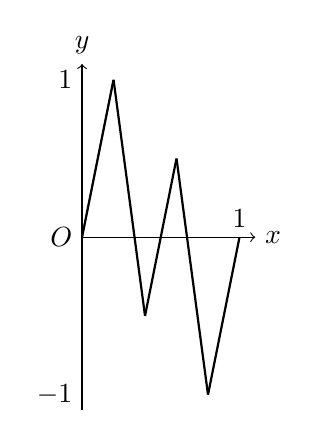
\begin{tikzpicture}[scale=2]
            \draw[->] (0,0) -- (1.1,0) node[right] {$x$};
            \draw[->] (0,-1.1) -- (0,1.1) node[above] {$y$};

            \node at (0,0) [left] {$O$};
            \node at (0,1) [left] {$1$};
            \node at (0,-1) [left] {$-1$};
            \node at (1,0) [above] {1};

            \draw[domain=0:0.2,samples=20,smooth,thick,black]
            plot (\x,5*\x);
            \draw[domain=0.2:0.4,samples=20,smooth,thick,black]
            plot (\x,2.5-7.5*\x);
            \draw[domain=0.4:0.6,samples=20,smooth,thick,black]
            plot (\x,5*\x-2.5);
            \draw[domain=0.6:0.8,samples=20,smooth,thick,black]
            plot (\x,5-7.5*\x);
            \draw[domain=0.8:1,samples=20,smooth,thick,black]
            plot (\x,5*\x-5);
            \end{tikzpicture}
        \end{center}
        在$t\in(1,2)$时,我们构造的图像事实上与$\sin x$形状类似。
    \end{itemize}
}
\end{framed}

\begin{framed}
\begin{exercise}\label{sin inf zero}
    证明$\sin x=100(\sqrt{x+1}-\sqrt{x})$在$[0,+\infty)$上有无穷多个根。
\end{exercise}
\sol{
    记$f(x)=\sin x-100(\sqrt{x+1}-\sqrt{x})$,由于其为连续函数,只需找到为正的点与为负的点即可说明中间存在根。记$g(x)=-100(\sqrt{x+1}-\sqrt{x})$,有
    $$\lim_{x\to+\infty}g(x)=\lim_{x\to+\infty}\frac{-100}{\sqrt{x+1}+\sqrt{x}}=0$$
    从而存在$M>0$使得$x>M$时$|g(x)|<\frac{1}{2}$。取正整数$K$使得$2K\pi>M$,则利用三角不等式有当$k>K$时(此时$2k\pi>M$,从而下方的$g$绝对值都不超过$\frac{1}{2}$)
    $$f\bigg(2k\pi+\frac{\pi}{2}\bigg)=1+g\bigg(2k\pi+\frac{\pi}{2}\bigg)>\frac{1}{2}>0$$
    $$f\bigg(k\pi+\frac{3\pi}{2}\bigg)=-1+g\bigg(2k\pi+\frac{3\pi}{2}\bigg)<-\frac{1}{2}<0$$
    从而根据介值定理,$f$在$(2k\pi+\frac{\pi}{2},2k\pi+\frac{3\pi}{2})$一定存在一个根,而不同的$k$对应的上述区间\textbf{不重合},因此每个$k>K$都至少对应一个根,这就找到了无穷多个根。

    \note 利用介值定理研究根相关性质的题通常需要找为正、为负的点,而这一般依赖\textbf{作出草图观察并分析}。不过,
}
\end{framed}

从上面这些题目中,我们可以看到,虽然介值定理的应用可以非常灵活,它的基本思路往往是\textbf{对具体函数从图像入手研究}、\textbf{对抽象函数从简单情况出发}。之后的函数相关题目中我们仍然会使用这类技巧。

\subsubsection{函数迭代}
此外,学了函数后,我们也可以解决一类数列极限问题,也就是满足形如$a_n=f(a_{n-1},a_{n-2},\dots,a_{n-k})$的递推式的数列,称为\textbf{迭代数列}。

考虑一阶迭代$a_{n+1}=f(a_n)$,若$f$是一个连续函数,且\textbf{已知$a_n$极限存在},设它为$a$可以\textbf{两侧同取极限}得到(注意$a_{n+1}$与$a_n$极限均为$a$,这可由定义直接得到)
$$a=f(a)$$
由此,对于迭代数列的极限问题,只要证明了极限存在,计算极限往往是简单的。事实上,我们将满足$x=f(x)$的$x$称为$f$的\textbf{不动点},计算迭代数列极限往往归结为求$f$\textbf{不动点}、\textbf{证明存在性}、多个不动点时\textbf{判断落在哪个}三步。

\note 之所以先求不动点再证明存在性,是因为不动点位置可以给存在性证明提供思路。

我们将以不同类型的例子说明迭代数列的可能操作方式,首先是直接算出极限的例子:
\begin{framed}
\begin{exercise}
    考虑数列$a_n$满足
    $$a_{n+2}=aa_{n+1}+ba_n$$
    给出$a_n$存在非零极限的充要条件(用$a$、$b$、$a_0$、$a_1$的关系式表达)。
\end{exercise}
\sol{
    由于已知$a_n$存在极限,设其为$l$,利用极限的加减乘除性质,两边同取极限得到
    $$l=al+bl$$
    由$l$非零即得至少需要$a+b=1$。

    代入$a=1-b$\ (尝试可发现这比$b=1-a$更好操作),我们有
    $$a_{n+2}=(1-b)a_{n+1}+ba_n$$
    向等比数列配凑可以得到
    $$a_{n+2}+ba_{n+1}=a_{n+1}+ba_n,\quad a_{n+2}-a_{n+1}=-b(a_{n+1}-a_n)$$
    两式分别可以推出
    $$a_{n+1}+ba_n=a_1+ba_0,\quad a_{n+1}-a_n=(-b)^{n-1}(a_1-a_0)$$

    由于$a_n$极限存在,应有
    $$\lim_{n\to\infty}(-b)^{n-1}(a_1-a_0)=\lim_{n\to\infty}(a_{n+1}-a_n)=l-l=0$$
    从而利用等比数列的极限性质可知$a_0=a_1$或$|b|<1$,分类讨论:
    \begin{itemize}
        \item 若$a_0=a_1$,代入可以发现$a_n=a_0$为常数,由此只要$a_0\ne0$即保证了$a_n$极限为非零常数。
        \item 若$|b|<1$,此时$b\ne-1$,可从两递推式解出
        $$a_n=\frac{1}{b+1}(a_1+ba_0-(-b)^{n-1}(a_1-a_0))$$
        从而直接计算可知
        $$\lim_{n\to\infty}a_n=\frac{a_1+ba_0}{b+1}$$
        由此此时只要$a_1+ba_0\ne0$即符合要求。
    \end{itemize}

    综合以上,上式极限存在非零当且仅当$a+b=1$、$a_0=a_1$、$a_0\ne0$,或$a+b=1$、$|b|<1$、$a_1+ba_0\ne0$。

    \note 这是一个标准的极限操作和\textbf{基本代数处理}结合的例子,虽然使用的极限理论并不复杂,但想得到正确的结果还是需要对各种代数变形足够熟练的。
}
\end{framed}

接下来是两个使用标准分析过程的例子:
\begin{framed}
\begin{exercise}
    考虑数列$a_n$满足
    $$a_{n+1}=\sqrt{2a_n}$$
    对不同的$a_0\ge0$计算$a_n$的极限。
\end{exercise}
\sol{
    按照标准的三步过程进行:
    \begin{itemize}
        \item 设$f(x)=\sqrt{2x}$,则求解$x=\sqrt{2x}$可在$x\ge0$得到两个不动点0与2。
        \item 为了证明极限存在,我们往往需要通过\textbf{单调有界定理},具体来说可以归纳得到:
        \begin{enumerate}
            \item 当$a_0=0$时,$a_n$恒为0,极限为0;
            \item 当$0<a_0<2$时,有$a_n<a_{n+1}<2$,从而单调上升且有界$[0,2]$,极限存在;
            \item 当$a_0=2$时,$a_n$恒为2,极限为2;
            \item 当$a_0>2$时,有$a_n>a_{n+1}>2$,从而单调下降且有界$[2,a_0]$,极限存在。
        \end{enumerate}
        \item 上面的第一、第三种情况已经得到了极限,第二种情况由于$a_n\ge a_0>0$恒成立,由极限保序性可知极限大于0,又由不动点只有0和2,排除了0后只能为2;同理,第四种情况由于$a_n>2$恒成立,即可知极限至少为2,因此只能为2。
    \end{itemize}

    \note 这题是迭代数列估算的最基本过程。
}
\end{framed}

\begin{framed}
\begin{exercise}\label{sin ord}
    考虑数列$a_n$满足
    $$a_{n+1}=\sin a_n$$
    证明
    $$\lim_{n\to\infty}a_n=0$$
    \extra:计算
    $$\lim_{n\to\infty}\sqrt{n}a_n$$
\end{exercise}
\sol{
    \begin{itemize}
        \item \textbf{极限为0}
        
        在之前介绍三角函数时我们已经得到了估算,在$x\ne0$时$|\sin x|<|x|$,由此$\sin x=x$只有$x=0$一个解,也即原函数只有一个不动点。

        另一方面,由上述估算可知$|a_{n+1}|=|\sin a_n|\le|a_n|$,从而$|a_n|$单调有界,极限存在。进一步讨论,对于任何$a_1$,由于$a_2\in[-1,1]$,由三角函数性质有$\sin a_2$与$a_2$同号,以此归纳可知从第二项开始$a_n$恒不变号,再由$|a_n|$极限存在即得$a_n$极限存在,由不动点唯一得证极限为0。

        \item \textbf{阶数估算}
        
        \note 这部分较有技巧性,但可以\textbf{用于几乎所有迭代数列的收敛阶估算}。

        首先,要计算$\sqrt{n}a_n$的极限,利用初等函数连续性只需计算
        $$\lim_{n\to\infty}\frac{1}{na_n^2}$$
        再取倒数后求平方根即可。

        之所以要化成这样的式子,是为了利用\textbf{数列平均极限}的结论(见\exref{cesaro diff}中的版本),将上述极限看成$\frac{a_n^{-2}}{n}$,从而只要计算出
        $$\lim_{n\to\infty}(a_{n+1}^{-2}-a_n^{-2})$$
        就可以得到原极限。此时我们再代入表达式并通分得到
        $$\lim_{n\to\infty}(a_{n+1}^{-2}-a_n^{-2})=\lim_{n\to\infty}\frac{a_n^2-\sin^2a_n}{a_n^2\sin^2a_n}$$
        由于已知$n\to\infty$时$a_n\to0$,利用归结原理我们只需要计算
        $$\lim_{x\to0}\frac{x^2-\sin^2x}{x^2\sin^2x}$$
        进行等价无穷小替换可将分母写为$x^4$,进一步得到
        $$\lim_{x\to0}\frac{x+\sin x}{x}\frac{x-\sin x}{x^3}=2\lim_{x\to0}\frac{x-\sin x}{x^3}=\frac{1}{3}$$
        这里最后一步用了$x-\sin x$的渐近结果,可以暂且作为结论使用,学到微分中值定理后将有比较好的方式进行证明。

        由此即得
        $$\lim_{n\to\infty}\frac{1}{na_n^2}=\frac{1}{3}$$
        从而
        $$\lim_{n\to\infty}\sqrt{n}a_n=\sqrt{3}$$

        \note 注意这里将$\frac{1}{na_n^2}$转化为$a_{n+1}^{-2}-a_n^{-2}$与将数列极限转化为函数极限都\textbf{只能单向进行},也即算出后面可得前面,但算出前面是得不到后面的。
    \end{itemize}
}
\end{framed}

虽然刚才两个例子中的$a_n$都有整体单调性,$a_n$不是单调数列时我们仍然可能可以得到结果:
\begin{framed}
\begin{exercise}
    考虑数列$a_n$满足
    $$a_{n+1}=ba_n(1-a_n)$$
    且$a_1=\frac{1}{2}$、$b\in(2,3]$,计算
    $$\lim_{n\to\infty}a_n$$
\end{exercise}
\sol{
    我们先进行不动点的分析。求解$x=bx(1-x)$可以得到两个根$x=0$与$x=1-\frac{1}{b}$,由此极限若存在只能是二者中的一个。不过,试着取定$b$计算几项即可发现这里的$a_n$并不具有单调性,由此需要更好的方法。这题最重要的观察在于,计算后可以发现$a_n$\textbf{奇数项单调增}、\textbf{偶数项单调减},且\textbf{任何一个奇数项小于任何一个偶数项}。接下来的过程分为几步:
    \begin{itemize}
        \item \textbf{子列有界性}
        
        记$f(x)=bx(1-x)$,注意条件$b\in(2,3]$,作出图像观察后可以利用二次函数知识证明(这里$\frac{b}{4}$是$f(x)$的最大值,在$\frac{1}{2}$取到):
        $$\forall x\in\bigg[\frac{1}{2},1-\frac{1}{b}\bigg),\quad f(x)\in\bigg(1-\frac{1}{b},\frac{b}{4}\bigg]$$
        $$\forall x\in\bigg(1-\frac{1}{b},\frac{b}{4}\bigg],\quad f(x)\in\bigg[\frac{1}{2},1-\frac{1}{b}\bigg)$$

        \note 第二个式子的$x$取$\frac{b}{4}$侧需要证明$b\in[2,3)$时$\frac{b^2}{4}(1-\frac{b}{4})\ge\frac{1}{2}$,虽然左侧减右侧是一个三次函数,但尝试出在$b=2$时取等后可直接因式分解得到结论。

        \note 虽然得到这一步的过程相对复杂,但有了明确的\textbf{目标}后,接下来都是高考范围的代数处理过程。

        由此,利用$a_1=\frac{1}{2}$可知$a_2\in(1-\frac{1}{b},\frac{b}{4}]$,进一步得到$a_3\in[\frac{1}{2},1-\frac{1}{b})$,以此进行下去即可得到对任何正整数$k$有
        $$a_{2k-1}\in\bigg[\frac{1}{2},1-\frac{1}{b}\bigg)$$
        $$a_{2k}\in\bigg(1-\frac{1}{b},\frac{b}{4}\bigg]$$
        这就得到了奇数项、偶数项子列分别有界,且奇数项一定小于偶数项。

        \item \textbf{子列单调性}
        
        为了证明奇数项与偶数项的单调性,我们需要考虑$a_{n+2}$与$a_n$的关系,代入可知
        $$a_{n+2}=b^2a_n(1-a_n)(1-ba_n(1-a_n))$$
        记$g(x)=f(f(x))=b^2x(1-x)(1-bx(1-x))$。虽然$g(x)-x$是一个四次方程,但$f(x)=x$时有$g(x)=x$,因此我们已经知道了$g(x)-x$的两个根0与$1-\frac{1}{b}$,由此进一步分解可知
        $$g(x)-x=x(bx-b+1)(-b^2x^2+b(b+1)x-(b+1))$$
        计算可发现$-b^2x^2+b(b+1)x-(b+1)$没有根,其在$\rb$上恒小于0,由此即得$g(x)-x$当且仅当在$(0,1-\frac{1}{b})$为正。

        进一步估算可以发现(这里的代数计算相对复杂,省略具体过程,有兴趣的同学可以作图研究)
        $$\forall x\in\bigg[\frac{1}{2},1-\frac{1}{b}\bigg),\quad x<g(x)<1-\frac{1}{b}$$
        $$\forall x\in\bigg(1-\frac{1}{b},\frac{b}{4}\bigg],\quad x>g(x)>1-\frac{1}{b}$$
        由此,结合前一部分估算即可发现
        $$a_{2k-1}<g(a_{2k-1})=a_{2k+1}<1-\frac{1}{b}$$
        $$a_{2k}>g(a_{2k})=a_{2k+2}>1-\frac{1}{b}$$
        由此即证明了奇数项单调减、偶数项单调增。

        \item \textbf{极限计算}
        
        结合前两部分的单调与有界可知$a_{2k-1}$、$a_{2k}$极限均存在。由于$g(x)$不动点只有0与$1-\frac{1}{b}$,且奇数项、偶数项均恒大于等于$\frac{1}{2}$,极限不可能为0,即得
        $$\lim_{k\to\infty}a_{2k-1}=\lim_{k\to\infty}a_{2k}=1-\frac{1}{b}$$
        至此由定义可最终证明
        $$\lim_{n\to\infty}a_n=1-\frac{1}{b}$$
    \end{itemize}

    \note 一般来说,迭代数列的题目如果难以直接计算且本身不单调,往往可以分成具有不同单调性且趋于同一极限的部分,虽然会更加复杂,但本质是不难的。
}

\end{framed}
\subsection{定义}
\subsubsection{导数的运算}
导数的定义本身是十分简洁的,$f$在$x$处的导数也即
$$\lim_{h\to 0}\frac{f(x+h)-f(x)}{h}$$
由于连续的定义是分子极限为0,我们利用乘积极限可直接得到\textbf{可导必定连续}。不过,从这个定义出发衍生的运算律可能并不简单,我们证明两个相对复杂的情况作为函数极限的应用:
\begin{framed}
\begin{exercise}
    证明\textbf{除法求导}法则:若$f$、$g$在$(a,b)$可导,且$g$在$(a,b)$非零,则$x\in(a,b)$时
    $$\frac{\dr}{\dr x}\frac{f(x)}{g(x)}=\frac{f'(x)g(x)-g'(x)f(x)}{g^2(x)}$$
\end{exercise}
\sol{
    也即我们要计算
    $$\lim_{h\to0}\frac{1}{h}\bigg(\frac{f(x+h)}{g(x+h)}-\frac{f(x)}{g(x)}\bigg)=\lim_{h\to0}\frac{f(x+h)g(x)-g(x+h)f(x)}{hg(x+h)g(x)}$$
    由于$g(x)\ne0$,利用乘除极限可知将分母中的$g(x+h)$替换为$g(x)$不会影响极限情况,由此可将极限写成
    $$\frac{1}{g^2(x)}\lim_{h\to0}\frac{f(x+h)g(x)-g(x+h)f(x)}{h}$$
    为了凑出$f'(x)$与$g'(x)$对应的形式,我们在中间加减项将极限写为
    $$\frac{1}{g^2(x)}\lim_{h\to0}\frac{(f(x+h)g(x)-f(x)g(x))-(g(x+h)f(x)-f(x)g(x))}{h}$$
    由于已知$f'(x)$与$g'(x)$存在,利用乘积的极限即得上式为
    $$\frac{1}{g^2(x)}\bigg(g(x)\lim_{h\to0}\frac{f(x+h)-f(x)}{h}-f(x)\lim_{h\to0}\frac{g(x+h)-g(x)}{h}\bigg)$$
    由$f'(x)$、$g'(x)$定义得结论成立。
}
\end{framed}

\begin{framed}
\begin{exercise}
    证明\textbf{复合函数求导}的链式法则:若$g$在$(a,b)$可导,且值域在$(c,d)$中,$f$在$(c,d)$可导,则$t\in(a,b)$时
    $$\frac{\dr f(g(t))=}{\dr t}f'(g(t))g'(t)$$
    以此证明\textbf{反函数求导}法则,即若$f$、$g$可导且互为反函数,$g'(f(x))$非零的点有
    $$f'(x)=\frac{1}{g'(f(x))}$$
\end{exercise}
\sol{
    我们先写出定义
    $$\lim_{t\to0}\frac{f(g(t+h))-f(g(t))}{h}$$
    为了凑出$f$与$g$导数的形式,我们希望能将它看成
    $$\lim_{t\to0}\frac{f(g(t+h))-f(g(t))}{g(t+h)-g(t)}\frac{g(t+h)-g(t)}{h}$$
    但此做法\textbf{无法保证新出现的分母非零},由此需要分类讨论:
    \begin{itemize}
        \item 若存在$\delta>0$使得$0<|h|<\delta$时$g(t+h)\ne g(t)$恒成立,则我们的确可以将极限改写为
        $$\lim_{t\to0}\frac{f(g(t+h))-f(g(t))}{g(t+h)-g(t)}\frac{g(t+h)-g(t)}{h}$$
        第二部分极限为$g'(t)$,而换元$s=g(t+h)-g(t)$可得
        $$\lim_{t\to0}\frac{f(g(t+h))-f(g(t))}{g(t+h)-g(t)}=\lim_{s\to0}\frac{f(g(t)+s)-f(g(t))}{s}=f'(g(t))$$
        从而由乘积极限得证。
        \item 若对任何$\delta>0$,都存在$0<|h|<\delta$使得$g(t+h)=g(t)$,又要分为三步:
        
        \begin{enumerate}
            \item 我们先说明$g'(t)=0$。
            
            取$\delta=\frac{1}{n}$,则存在$|h_n|<\frac{1}{n}$使得$g(t+h_n)=g(t)$,从而
            $$\lim_{n\to\infty}\frac{g(t+h_n)-g(t)}{h_n}=0$$
            利用\textbf{归结原理},由定义$h_n$极限为0,于是上述极限必然与函数极限$g'(t)$相同,这就证明了$g'(t)=0$。由此,目标变为证明
            $$\lim_{t\to0}\frac{f(g(t+h))-f(g(t))}{h}=0$$

            \note 注意此时无法取$h=h_n$说明,因为\textbf{不确定函数极限存在时无法通过单个数列确定}。

            \item 由于已知
            $$\lim_{t\to0}\frac{g(t+h)-g(t)}{h}=0$$
            我们希望存在$M$、$\delta>0$使得$h\in(-\delta,\delta)$时
            $$|f(g(t+h))-f(g(t))|\le M|g(t+h)-g(t)|$$
            这样即能通过$h\in(-\delta,\delta)$时
            $$\bigg|\frac{f(g(t+h))-f(g(t))}{h}\bigg|\le M\bigg|\frac{g(t+h)-g(t)}{h}\bigg|$$
            即
            $$-M\bigg|\frac{g(t+h)-g(t)}{h}\bigg|\le\frac{f(g(t+h))-f(g(t))}{h}\le M\bigg|\frac{g(t+h)-g(t)}{h}\bigg|$$
            由夹逼定理直接得到中间极限为0。

            \item 最后我们证明上述的$M$与$\delta$的确存在。注意到我们仍然没有用到$f$的导数的条件,这里自然需要使用$f$的导数进行估算。
            
            由于$f'(g(t))$存在,设$L=|f'(g(t))|$,利用绝对值函数连续性有
            $$\lim_{s\to0}\bigg|\frac{f(g(t)+s)-f(g(t))}{s}\bigg|=L$$
            利用极限\textbf{保序性}可知存在$\delta_0>0$使得$s\in(-\delta_0,0)\cup(0,\delta_0)$时
            $$\bigg|\frac{f(g(t)+s)-f(g(t))}{s}\bigg|<L+1$$
            从而同乘$h$,结合0处两侧相等即得$s\in(-\delta_0,\delta_0)$时
            $$|f(g(t)+s)-f(g(t))|\le(L+1)|s|$$
            利用$g$可导,其在$t$处连续,从而存在$\delta$使得$h\in(-\delta,\delta)$时$|g(t+h)-g(t)|<\delta_0$,从而$h\in(-\delta,\delta)$时
            $$|f(g(t)+(g(t+h)-g(t)))-f(g(t))|\le(L+1)|g(t+h)-g(t)|$$
            也即
            $$|f(g(t+h))-f(g(t))|\le(L+1)|g(t+h)-g(t)|$$
            取$M=L+1$即找到了符合要求的$M$与$\delta$。

            \note 将过程中的1改成任何大于0的$\varepsilon$都能推出小于等于号成立,由此事实上将这一步过程改造可以直接证明极限为$f'(g(t))g'(t)$,不过讨论方式会相对复杂。
        \end{enumerate}

    \end{itemize}
}
\end{framed}

有了这些运算律后,利用基本的等价无穷小结论可以算出基本初等函数的导数,进而得到所有初等函数的导数计算方式,讨论可得结论\textbf{初等函数若在开区间可导则导数仍为初等函数}。

\note 注意初等函数未必在连续点可导,如$|x|=\sqrt{x^2}$是初等函数,但在0处并不可导。

此外,关于导数的一些基本性质将会变得很容易证明:
\begin{framed}
\begin{exercise}
    证明可导的奇函数导数为偶函数,可导的偶函数导数为奇函数,可导的周期函数导数为周期函数。

    若$f$为$\rb$上可导的函数,且$f'(x)$有周期$T$,即$f'(x+T)=f'(x)$,是否$f$一定有周期$T$?
\end{exercise}
\sol{
    \begin{itemize}
        \item \textbf{可导的奇函数导数为偶函数}
        
        由条件$f(-x)=-f(x)$,两侧同时求导由复合函数求导法则即得$-f'(-x)=-f'(x)$,即$f'(-x)=f'(x)$。

        \item \textbf{可导的偶函数导数为奇函数}
        
        由条件$f(-x)=f(x)$,两侧同时求导由复合函数求导法则即得$-f'(-x)=f'(x)$,即$f'(-x)=-f'(x)$。

        \item \textbf{可导的周期函数导数为周期函数}
        由条件存在$T$使得$f(x+T)=f(x)$,两侧同时求导由复合函数求导法则即得$f'(x+T)=f'(x)$,从而$f'(x)$以$T$为周期。

        \item \textbf{导数为周期函数不能推出原函数为周期函数}
        
        考虑$f(x)=x$,$f'(x)=1$以任意正实数为周期,但$f(x)$不是周期函数。
    \end{itemize}
}

\end{framed}

不过,到这里,我们需要讨论一个从几何直观来看不算平凡的事:$f(x)$在一点处趋于无穷和它的导数趋于无穷是\textbf{完全不同}的概念:
\begin{framed}
\begin{exercise}[\extra]
    举例说明,若$f$在$(a,b)$可导
    $$\lim_{x\to b^-}f(x)=+\infty,\quad\lim_{x\to b^-}f'(x)=+\infty$$
    互相无法推出。
\end{exercise}
\sol{
    \begin{itemize}
        \item \textbf{导数趋于正无穷而函数有限}
        
        考虑区间$(0,1)$上的$f(x)=-\sqrt{1-x}$,直接计算有
        $$f'(x)=\frac{1}{2\sqrt{1-x}}$$
        从而$x\to1^-$时$f'(x)\to+\infty$,而由初等函数连续性$f(x)\to0$。

        \item \textbf{函数趋于正无穷而导数极限不为正无穷}
        
        此例子的构造会稍复杂一些分为两步:
        \begin{enumerate}
            \item 先证明引理:对任何区间$[s,t]$与给定的$c$、$d$,存在三次函数$h$使得
            $$h(s)=c,\quad h(t)=d,\quad h'(s)=h'(t)=0$$

            由于$h'(x)$为二次函数且$h'(s)=h'(t)=0$,应有($C_1$为某常数)
            $$h'(x)=C_1(x-s)(x-t)$$
            从而考虑利用多项式的导数可发现($C_2$也为某常数)
            $$h(x)=\frac{1}{3}C_1x^3-\frac{1}{2}(s+t)C_1x^2+C_1stx+C_2$$
            由此代入剩下两个条件可得到关于$C_1$、$C_2$的方程
            $$\bigg(\frac{1}{6}s^3+\frac{1}{2}s^2t\bigg)C_1+C_2=c$$
            $$\bigg(\frac{1}{3}t^3+\frac{1}{2}st^2\bigg)C_1+C_2=d$$
            由于$s<t$,可发现第一个方程中$C_1$的系数小于第二个方程中$C_1$的系数,于是作差相消即可解出$C_1$,进一步代入得$C_2$。

            我们将$h(x)$称为\textbf{可导连接$(s,c)$与$(t,d)$}的曲线。可以进一步计算发现当$c<d$时它在$[s,t]$上\textbf{单调增加}。

            \note 事实上,利用多项式插值理论,即使要求$s$与$t$处直到$k$阶的导数都为0,也一定可以解出符合要求的多项式。

            \item 考虑区间$(0,1)$,任取$\varepsilon\in(0,1)$,构造$f(x)$满足对任何正整数$n$有
            $$\forall x\in\bigg(1-\frac{1}{n}+\frac{\varepsilon}{n(n+1)},1-\frac{1}{n+1}-\frac{\varepsilon}{n(n+1)}\bigg),\quad f(x)=n$$
            且$f(x)$在$(1-\frac{1}{n+1}-\frac{\varepsilon}{n(n+1)},n)$与$(1-\frac{1}{n+1}+\frac{\varepsilon}{(n+1)(n+2)},n+1)$之间是可导连接这两点的曲线。

            由此,利用引理可由导数定义发现$f$在所有分界点处的导数均为0,而其他点处$f(x)$均在附近为初等函数,因此导数存在。

            由引理可发现$f(x)$单调增加,且
            $$f\bigg(1-\frac{1}{n+1}\bigg)\ge n$$
            由此即利用定义得到
            $$\lim_{x\to1^-}f(x)=+\infty$$
            而由于
            $$f'\bigg(1-\frac{1}{n}+\frac{\varepsilon}{n(n+1)}\bigg)=0$$
            恒成立,令$n$趋于无穷可得
            $$\lim_{n\to\infty}f'\bigg(1-\frac{1}{n}+\frac{\varepsilon}{n(n+1)}\bigg)=0$$
            若$f'(x)$在$x\to1^-$时极限为正无穷,由推广的归结原理可知上述极限应为$+\infty$,从而矛盾。
        \end{enumerate}

        \note 本题事实上也是先画图再构造的,我们构造出了一个\textbf{不断增加但一直有平缓部分}的函数。事实上,$f(x)$的性质可能与$f'(x)$的性质差异很大,几乎不能通过几何直观得到结论。真正联系函数与其导数需要在学到\textbf{微分中值定理}后。
    \end{itemize}
}
\end{framed}

当然,上述的讨论只是对导数最基本的\textbf{代数}性质的刻画,接下来我们将谈论它的重要\textbf{几何}性质,也就是作为``切线''的几何意义。

\subsubsection{可导性与近似}
几何上来说,``切线''意味着一点附近最\textbf{接近}的一条直线,这也是我们高中学到的几何直观,它可以用如下的定理刻画:
\begin{framed}
\begin{exercise}
    若$f$在$x_0$处可导,设
    $$l_0(x)=f(x_0)+f'(x_0)(x-x_0)$$
    证明$l_0(x)$是$f(x)$在$x_0$附近的\textbf{最佳一次逼近},也即对任何一个一次函数$l(x)$,存在$\delta>0$使得$|x-x_0|<\delta$时
    $$|f(x)-l_0(x)|\le|f(x)-l(x)|$$
\end{exercise}
\sol{
    分两种情况讨论:
    \begin{itemize}
        \item 若$l(x_0)\ne f(x_0)$,我们可以直接通过连续性证明:记
        $$g(x)=|f(x)-l(x)|-|f(x)-l_0(x)|$$
        由$f(x_0)=l_0(x_0)$可发现$g(x_0)>0$,而由$f$在$x_0$处可导,其在$x_0$处连续,根据连续函数复合性质可知$g(x)$也在$x_0$处连续,从而由极限保号性存在$\delta>0$使得$0<|x-x_0|<\delta$时$g(x)>0$,再结合$g(x_0)>0$即得$|x-x_0|<\delta$时$g(x)>0$,得证。
        \item 若$l(x_0)=f(x_0)$,可设$l(x)=f(x_0)+k(x-x_0)$。我们写出现在的不等式形式
        $$|f(x)-f(x_0)-f'(x_0)(x-x_0)|\le|f(x)-f(x_0)-k(x-x_0)|$$
        由于无论$k$取何值,$x=x_0$时等号成立,两边同除以$|x-x_0|$,我们只需证明存在$\delta$使得$0<|x-x_0|<\delta$时
        $$\bigg|\frac{f(x)-f(x_0)}{x-x_0}-f'(x_0)\bigg|\le\bigg|\frac{f(x)-f(x_0)}{x-x_0}-k\bigg|$$
        记上式右减左为$h(x)$,若$k=f'(x_0)$,$h(x)$恒为0,已经成立,否则利用导数定义与复合函数极限结论可知
        $$\lim_{x\to x_0}h(x)=|f'(x_0)-k|-|f'(x_0)-f'(x_0)|=|f'(x_0)-k|>0$$
        从而再次由极限保号性得证存在上述$\delta$。
    \end{itemize}

    \note 本题的核心思路是从函数作差中\textbf{配凑}出导数的形式。
}
\end{framed}

从几何性质的思路出发,我们可以进行一些导数相关的\textbf{估算},这里只举三个不算复杂的例子:
\begin{framed}
\begin{exercise}
    若$|f(x)|\le|g(x)|$在$(-1,1)$恒成立,且$g$在0处可导,$g(0)=g'(0)=0$,证明$f$在0处可导并计算$f'(0)$。
\end{exercise}
\sol{
    由条件代入$x=0$可知$f(0)=0$,从而根据定义
    $$f'(0)=\lim_{x\to0}\frac{f(x)}{x}$$
    利用$|f(x)|\le|g(x)|$两边除以$|x|$可知$(-1,0)\cup(0,1)$上有
    $$-\bigg|\frac{g(x)}{x}\bigg|\le\frac{f(x)}{x}\le\bigg|\frac{g(x)}{x}\bigg|$$
    利用$g(x)$在0处导数为0的定义与复合函数的极限结论,左右在$x\to0$时极限都为0,由夹逼定理即得$f'(0)=0$.
}
\end{framed}

\begin{framed}
\begin{exercise}\label{deri not cont}
    设
    $$f(x)=\begin{cases}\ln(1+x)&x\in\mathbb{Q}\\\sin x&x\notin\mathbb{Q}\end{cases}$$
    计算$f'(0)$。
\end{exercise}
\sol{
    由于此函数并不具有任何直接的性质,我们只能由定义出发计算导数。由定义可发现$f(0)=0$,从而
    $$f'(0)=\lim_{x\to0}\frac{f(x)}{x}$$
    记$g(x)=\frac{f(x)}{x}$,它在0的\textbf{去心}邻域有定义,且满足
    $$g(x)=\begin{cases}\frac{\ln(1+x)}{x}&x\in\mathbb{Q}\\\frac{\sin x}{x}&x\notin\mathbb{Q}\end{cases}$$
    由于
    $$\lim_{x\to0}\frac{\ln(1+x)}{x}=\lim_{x\to0}\frac{\sin x}{x}=1$$
    对任何$\varepsilon>0$,存在$\delta$使得(对两种情况分别取$\delta$再取出较小的)只要$0<|x|<\delta$即有
    $$\bigg|\frac{\ln(1+x)}{x}-1\bigg|<\delta,\quad\bigg|\frac{\sin x}{x}-1\bigg|<\delta$$
    由于$g(x)$必然与上方两个中的某个相等即得$|g(x)-1|<\delta$,从而由定义得证
    $$\lim_{x\to0}g(x)=1$$
    也即$f'(0)=1$。

    \note 注意本题的方法可以推广到,若$f(x)$在$x_0$的一个邻域内每点等于$g(x)$或$h(x)$,且$g(x_0)=h(x_0)$、$g'(x_0)=h'(x_0)=t$,则必然有$f$在$x_0$可导且$f'(x_0)=t$。
}
\end{framed}
\note 注意此例子说明\textbf{一点处可导只能推出一点连续},此例子中的函数在0的任何邻域都不连续。

\begin{framed}
\begin{exercise}\label{ln deri approx}
    计算
    $$\lim_{n\to\infty}\bigg(\frac{1}{n+1}+\frac{1}{n+2}+\dots+\frac{1}{2n}\bigg)$$
\end{exercise}
\sol{
    利用基本等价无穷小可知(这实际上也是$\ln x$在1处的导数)
    $$\lim_{x\to0}\frac{\ln(1+x)-x}{x}=1-1=0$$
    由此,对任何$\varepsilon>0$,存在$\delta$使得$x\in(-\delta,0)\cup(0,\delta)$时
    $$\bigg|\frac{\ln(1+x)-x}{x}\bigg|<\varepsilon$$
    两边乘$|x|$后由0处相等可知$x\in(-\delta,\delta)$时
    $$|\ln(1+x)-x|\le\varepsilon|x|$$
    由此,取$N$使得$\frac{1}{N}<\delta$,即有$n>N$时
    $$\sum_{k=n+1}^{2n}\frac{1}{k}=\sum_{k=n+1}^{2n}\ln\bigg(1+\frac{1}{k}\bigg)+\sum_{k=n+1}^{2n}\bigg(\frac{1}{k}-\ln\bigg(1+\frac{1}{k}\bigg)\bigg)$$
    由于$\ln\big(1+\frac{1}{k}\big)=\ln(k+1)-\ln k$,裂项即得上式能写为
    $$\sum_{k=n+1}^{2n}\frac{1}{k}-\ln\frac{2n+1}{n}=\sum_{k=n+1}^{2n}\bigg(\frac{1}{k}-\ln\bigg(1+\frac{1}{k}\bigg)\bigg)$$
    由于上述所有$1/k$都在$(-\delta,\delta)$中,利用之前的估算可知
    $$\bigg|\sum_{k=n+1}^{2n}\frac{1}{k}-\ln\frac{2n+1}{n}\bigg|\le\sum_{k=n+1}^{2n}\frac{\varepsilon}{k}<\sum_{k=n+1}^{2n}\frac{\varepsilon}{n}=\varepsilon$$
    由此利用极限定义即得
    $$\lim_{n\to\infty}\bigg(\sum_{k=n+1}^{2n}\frac{1}{k}-\ln\frac{2n+1}{n}\bigg)=0$$
    而根据初等函数连续性与归结原理可知
    $$\lim_{n\to\infty}\ln\frac{2n+1}{n}=\lim_{n\to\infty}\ln\bigg(2+\frac{1}{n}\bigg)=\ln2$$
    于是
    $$\lim_{n\to\infty}\bigg(\frac{1}{n+1}+\frac{1}{n+2}+\dots+\frac{1}{2n}\bigg)=\ln2$$

    \note 这里的核心思路是,由于$\ln$求和容易裂项相消,我们希望说明此倒数和与$\ln$求和的差距可以在$n\to\infty$时趋于0。

    \note 本题也可以利用\exref{eular const}的结论,记$a_n$为$\sum_{k=1}^n\frac{1}{k}-\ln n$,由于$a_n$极限存在,$a_{2n}-a_n$极限为0,这样也能得到极限为$\ln2$,但上方的\textbf{导数估算}做法实际上是更加本质的:它无需利用我们尚未知道如何严谨证明的$\ln(1+x)\le x$结论。

    
}
\end{framed}

不过,这些几何角度的讨论还远远不是导数的全貌。例如,有了最佳一次逼近以后,我们是否能找到最佳二次、最佳三次,乃至最佳$n$次逼近?这些问题事实上也可以用导数来回答,也即导数\textbf{完全解决了}多项式逼近的问题。不过,我们在下半学期才能进行这一部分讨论,目前仍然只能以介绍计算技巧为主。

\subsection{计算}
\subsubsection{高阶导数}
由于基本初等函数的一阶导数是不难通过之前的极限计算的,初等函数的导数往往是非常简单的问题。因此,导数相关的困难计算经常会涉及\textbf{高阶导数},也就是进行多次求导运算(我们用\textbf{0阶导数}表示函数自身)。对于这类问题,涉及的技巧就相对灵活了。我们先给出几乎是这部分最重要的定理,\textbf{乘积的$n$阶导数}:
\begin{framed}
\begin{exercise}\label{mul n deri}
    若$f(x)$、$g(x)$均在$\rb$上$n$阶可导,计算$f(x)g(x)$对$x$的$n$阶导数,$n\in\mathbb{N}$。
\end{exercise}
\sol{
    尝试算前几项后可发现存在与二项式定理类似的系数,由此我们先\textbf{猜测}结果为
    $$\sum_{k=0}^nC_n^kf^{(k)}(x)g^{(n-k)}(x)$$
    这里上标$(k)$表示$k$阶导数,$k=0$时即表示函数自身。

    为了证明此结果,可以使用\textbf{归纳法}:当$n=1$时由乘积求导公式可知结论成立,若$n-1$时情况成立,$n$时有
    $$\frac{\dr^nf(x)g(x)}{\dr x^n}=\frac{\dr}{\dr x}\sum_{k=0}^{n-1}C_{n-1}^kf^{(k)}(x)g^{(n-1-k)}(x)$$
    将每一项用乘积求导公式展开可知
    $$\frac{\dr^nf(x)g(x)}{\dr x^n}=\sum_{k=0}^{n-1}C_{n-1}^k\big(f^{(k+1)}(x)g^{(n-1-k)}(x)+f^{(k)}(x)g^{(n-k)}(x)\big)$$
    注意两项的$f$的导数次数与$g$的导数次数和为$n$,我们可以进行拆分重组:
    $$\begin{aligned}\frac{\dr^nf(x)g(x)}{\dr x^n}&=\sum_{k=0}^{n-1}C_{n-1}^kf^{(k+1)}(x)g^{(n-1-k)}(x)+\sum_{k=0}^{n-1}C_{n-1}^kf^{(k)}(x)g^{(n-k)}(x)\\ &=\sum_{k=1}^nC_{n-1}^{k-1}f^{(k)}(x)g^{(n-k)}(x)+\sum_{k=0}^{n-1}C_{n-1}^kf^{(k)}(x)g^{(n-k)}(x)\\ &=f^{(n)}(x)g(x)+\sum_{k=1}^{n-1}(C_{n-1}^{k-1}+C_{n-1}^k)f^{(k)}(x)g^{(n-k)}(x)+f(x)g^{(n)}(x)\end{aligned}$$

    \note 上方第二个等号是将第一个求和中的$k+1$替换为新的$k$;第三个等号是将相同的$k$合并,留下第一个求和中$k=n$的项与第二个求和中$k=0$的项。

    对比此式与我们证明目标的系数,可发现只需证明
    $$C_{n-1}^{k-1}+C_{n-1}^k=C_n^k$$
    而这可以直接通过定义得到:
    $$\begin{aligned}C_{n-1}^{k-1}+C_{n-1}^k&=\frac{(n-1)!}{(k-1)!(n-k)!}+\frac{(n-1)!}{k!(n-k-1)!}\\ &=\frac{(n-1)!}{(k-1)!(n-k-1)!}\bigg(\frac{1}{n-k}+\frac{1}{k}\bigg)\\ &=\frac{(n-1)!}{(k-1)!(n-k-1)!}\frac{n}{(n-k)k}\\ &=\frac{n!}{k!(n-k)!}=C_n^k\end{aligned}$$
    从而证明了原结论。
}

\end{framed}

利用它可以进行一些计算:
\begin{framed}
\begin{exercise}
    计算$f(x)=\arctan x$在0处的$n$阶导数值,$n\in\mathbb{N}$。
\end{exercise}
\sol{
    提供两种方法:
    \begin{itemize}
        \item 由于$\arctan$难以直接操作,我们先尝试求一次导数得到
        $$f'(x)=\frac{1}{1+x^2}$$
        此时右侧成为两个多项式的商,但仍然难以处理,我们试着两侧\textbf{同乘}$1+x^2$得到
        $$f'(x)(1+x^2)=0$$
        由于$1+x^2$求3阶及以上导数为0,当$n\ge3$时,对左侧求$n-1$阶导可以利用\exref{mul n deri}展开,从而得到
        $$f^{(n)}(x)(1+x^2)+C_{n-1}^1f^{(n-1)}(x)\cdot(2x)+C_{n-1}^2f^{(n-2)}(x)\cdot 2=0$$
        代入$x=0$即可计算得到
        $$f^{(n)}(0)+(n-1)(n-2)f^{(n-2)}(0)=0$$
        由此利用直接计算的结论$f(0)=0$、$f'(0)=1$、$f''(0)=0$递推可得到
        $$f^{(2k)}(0)=0,\quad k\in\mathbb{N}$$
        $$f^{(2k+1)}(0)=(-1)^k(2k)!,\quad k\in\mathbb{N}$$

        \item (\extra)仍然从求一阶导后的结果
        $$f'(x)=\frac{1}{1+x^2}$$
        出发。
        
        \note 由于我们尚未学过复函数相关的理论与导数含义,\textbf{此方法直接使用将被扣分},但可以用于提供思路与结果。

        利用复数知识可以计算验证
        $$x^2+1=(x-\ir)(x+\ir)$$
        从而进一步计算有
        $$\frac{1}{1+x^2}=\frac{1}{2\ir}\bigg(\frac{1}{x-\ir}-\frac{1}{x+\ir}\bigg)$$
        直接计算可发现
        $$\bigg(\frac{1}{x+c}\bigg)^{(n-1)}=\frac{(-1)^{n-1}(n-1)!}{(x+c)^n}$$
        对任何实数$c$成立,我们\textbf{形式上}认为对复数也成立,从而写出导数
        $$\bigg(\frac{1}{1+x^2}\bigg)^{(n-1)}=\frac{(-1)^{n-1}(n-1)!}{2\ir}\bigg(\frac{1}{(x-\ir)^n}-\frac{1}{(x+\ir)^n}\bigg)$$

        \note 事实上利用复变函数知识可以证明,右侧的确是$\frac{1}{1+x^2}$的$n-1$阶导数。

        从而可知
        $$f^{(n)}(0)=\frac{(-1)^{n-1}(n-1)!}{2\ir}\bigg(\frac{1}{(-\ir)^n}-\frac{1}{\ir^n}\bigg)$$
        由于$\ir(-\ir)=1$,我们可以化简得到
        $$f^{(n)}(0)=\frac{(-1)^{n-1}(n-1)!}{2\ir}(\ir^n-(-1)^n\ir^n)=\frac{(-1)^{n-1}(n-1)!}{2}(1-(-1)^n)\ir^{n-1}$$
        由此即可进一步算得
        $$f^{(2k)}(0)=0,\quad k\in\mathbb{N}$$
        $$f^{(2k+1)}(0)=(-1)^k(2k)!,\quad k\in\mathbb{N}$$
    \end{itemize}
}

\end{framed}
\begin{framed}
\begin{exercise}[\extra]
    计算$f(x)=\arcsin x$在0处的$n$阶导数值,$n\in\mathbb{N}$。
\end{exercise}
\sol{
    与之前类似先求一阶导得到
    $$f'(x)=\frac{1}{\sqrt{1-x^2}}$$
    直接相乘可得
    $$\sqrt{1-x^2}f'(x)=1$$
    但若直接两边平方后求$n-1$阶导,从$(f'(x))^2$的$n$阶导数难以直接解出$f^{(n-1)}(x)$,我们需要寻找更好的方法。

    尝试再求一阶导得到
    $$f''(x)=\frac{x}{(1-x^2)^{3/2}}$$
    由此可发现
    $$f''(x)=\frac{x}{(1-x^2)}f'(x)$$
    将其改写为
    $$(1-x^2)f''(x)-xf'(x)=0$$
    即可以类似之前进行操作了。当$n\ge4$时两边同求$n-2$阶导有($1-x^2$三阶及以上导数为0,$x$二阶及以上导数为0)
    $$(1-x^2)f^{(n)}(x)+C_{n-2}^1(-2x)f^{(n-1)}(x)+C_{n-2}^2(-2)f^{(n-2)}(x)-(xf^{(n-1)}(x)+C_{n-2}^1f^{(n-2)}(x))=0$$
    代入$x=0$即发现
    $$f^{(n)}(0)-(n-2)^2f^{(n-2)}(0)=0$$
    由此计算$f(0)=0$、$f'(0)=1$、$f''(0)=0$递推可得到
    $$f^{(2k)}(0)=0,\quad k\in\mathbb{N}$$
    $$f^{(2k+1)}(0)=1^23^25^2\dots(2k-1)^2,\quad k\in\mathbb{N}^*$$
    \note 一种记号是将$1^23^25^2\dots(2k-1)^2$写作$(2k-1)!!$。
}
\end{framed}

不过,对于更一般的问题,往往需要自己逐步求导观察,我们先用\exref{poly exp}的结论给出一个函数构造并计算导数:
\begin{framed}
\begin{exercise}\label{poly exp n deri}
    设
    $$f(x)=\begin{cases}0&x=0\\\er^{-1/x^2}&x\ne0\end{cases}$$
    计算$f(x)$在0处的$n$阶导数值,这里$n\in\mathbb{N}$。
\end{exercise}
\sol{
    我们先证明$\er^{-1/x^2}$在0以外的点的$n$阶导数($n\in\mathbb{N}$)一定可以写为
    $$\frac{f(x)}{x^M}\er^{-1/x^2}$$
    其中$f$为多项式,$M$为某自然数。

    直接归纳即可:当$n=0$时0阶导数即为自身$\er^{-1/x^2}$,从而成立,若$n-1$阶导数能写为此形式,再次求导计算可发现
    $$\bigg(\frac{f(x)}{x^M}\er^{-1/x^2}\bigg)'=\bigg(\frac{f'(x)x^M-Mx^{M-1}f(x)}{x^{2M}}+\frac{2f(x)}{x^{M+5}}\bigg)\er^{-1/x^2}$$
    利用多项式的导数还是多项式通分即可得到结论。

    我们接下来\textbf{归纳}证明$f$在0处的$n$阶导数为0。由定义可知$f(0)=0$,若结论对$n-1$阶导数成立,利用归纳假设可知
    $$f^{(n-1)}(x)=\begin{cases}0&x=0\\\frac{f(x)}{x^M}\er^{-1/x^2}&x\ne0\end{cases}$$
    由此可知
    $$f^{(n)}(0)=\lim_{x\to0}\frac{\frac{f(x)}{x^M}\er^{-1/x^2}-0}{x}=\lim_{x\to0}\frac{f(x)}{x^{M+1}}\er^{-1/x^2}$$
    利用\exref{poly exp}的结论即可得到此极限为0,从而得证。

    \note 此证明的核心思路事实上在下半学期才能学到来源:若$f(x)$在0处的0到$n-1$阶导均为0,而$n$阶导非零,可以证明$x\to0$时$f(x)$与$x^n$是\textbf{同阶}无穷小。由于$\er^{-1/x^2}$在$x\to0$时将比任何多项式趋于0的速度都快(\exref{poly exp}已经证明),必然$f(x)$的任意阶导数均为0。

    \note 此函数是\textbf{光滑但不实解析}的函数的重要例子。光滑是指可以求任意阶导数,实解析的概念我们将在后半学期介绍。
}
\end{framed}

最后,我们再看一个直接计算导数进行递推的例子:
\begin{framed}
\begin{exercise}
    对正整数$n$,设$f_n(x)=x^n\ln x$,求
    $$\lim_{n\to\infty}\frac{f_n^{(n)}(1/n)}{n!}$$
\end{exercise}
\sol{
    尝试求一次导可以发现
    $$f_n'(x)=x^{n-1}+nx^{n-1}\ln x=x^{n-2}+nf_{n-1}(x)$$
    由此再求$n-1$阶导,直接归纳计算可发现$x^{n-1}$的$n-1$阶导是$(n-1)!$,从而
    $$f_n^{(n)}(x)=(n-1)!+nf_{n-1}^{(n-1)}(x)$$
    为了凑出题目中的形式,我们除以$n!$研究,即可发现
    $$\frac{f_n^{(n)}(x)}{n!}=\frac{1}{n}+\frac{f_{n-1}^{(n-1)}(x)}{(n-1)!}$$
    由此递推即得
    $$\frac{f_n^{(n)}(x)}{n!}=\frac{1}{n}+\frac{1}{n-1}+\dots+\frac{1}{2}+f_1'(x)$$
    进一步计算可得
    $$\frac{f_n^{(n)}(x)}{n!}=\frac{1}{n}+\frac{1}{n-1}+\dots+\frac{1}{2}+1+\ln x$$
    于是可知
    $$\frac{f_n^{(n)}(1/n)}{n!}=\frac{1}{n}+\frac{1}{n-1}+\dots+\frac{1}{2}+1-\ln n$$
    其极限为\textbf{欧拉常数}(定义见\exref{eular const})。
}
\end{framed}

\subsubsection{隐函数与参数曲线}
除了这类问题外,另一类常见的计算性问题是,函数\textbf{并不显式给出},而是藏在方程或参数中。我们以两个例题说明这种情况下的计算该如何进行。首先是隐函数的情况:
\begin{framed}
\begin{exercise}
    设$y=f(x)$是由
    $$x^2+y^2+xy=1$$
    确定的可导函数,计算$f''(x)$。
\end{exercise}
\sol{
    对于隐函数问题,一个最简单的方法是直接\textbf{对等式两侧求导}得到
    $$2x+2f(x)f'(x)+xf'(x)+f(x)=0$$
    可以发现已经成为了对$f'(x)$的一元一次函数,从而得到($2y+x\ne0$时)
    $$f'(x)=-\frac{2x+y}{2y+x}$$
    
    \note 注意如果不想把$y$写成$f(x)$,求导时一定不要忘记\textbf{$y$是$x$的函数},因此需要利用复合函数求导。

    接下来直接用商求导公式即得到($2y+x\ne0$时)
    $$f''(x)=-\frac{(2+f'(x))(2y+x)-(2f'(x)+1)(2x+y)}{(2y+x)^2}$$
    再代入$f'(x)$表达式化简即得($2y+x\ne0$时)
    $$f''(x)=-6\frac{x^2+xy+y^2}{(2y+x)^3}$$
    再由条件$x^2+xy+y^2=1$可进一步化简结果为($2y+x\ne0$时)
    $$f''(x)=-\frac{6}{(2y+x)^3}$$

    \note 严格来说,我们还需要判断$2y+x=0$时是否的确不可导,不过这类题目一般不需要进行如此严格的讨论。事实上,可以证明导数分母为0时,若分子非零,曲线往往\textbf{切线与$y$轴垂直},从而的确斜率不存在。
}
\end{framed}

若隐函数的形式是$g(x,y(x))=0$,利用复合函数求导公式,两侧对$x$求导可以得到(我们将在下半学期介绍更多知识后\textbf{证明})
$$0=\frac{\dr}{\dr x}g(x,y)=\frac{\partial g(x,y)}{\partial x}+\frac{\partial g(x,y)}{\partial y}y'(x)$$
这里的$\frac{\partial}{\partial x}$表示将$y$看为常数时$g(x,y)$对$x$求导的结果,$\frac{\partial}{\partial y}$表示将$x$看为常数时$g(x,y)$对$y$求导的结果。由此结果\textbf{一定是}关于$y'(x)$的一元一次方程,两边求导的方法是可以通用的。

\

接下来是参数方程的情况:
\begin{framed}
\begin{exercise}
    设$y=f(x)$是由
    $$\begin{cases}x=\ln(1+t^2)\\y=t-\arctan t\end{cases}$$
    确定的函数,计算$f''(x)$。
\end{exercise}
\sol{
    由于$x$是$t$的函数,上述两式事实上可以改写为
    $$\begin{cases}x(t)=\ln(1+t^2)\\f(x(t))=t-\arctan t\end{cases}$$
    由此利用复合函数求导公式即得(注意下式中第一个、第三个求导是对$t$,第二个求导是对$x$,这样写是没有歧义的,因为$f$是$x$的函数,而$f(x(t))$与$x(t)$都是$t$的函数)
    $$(f(x(t)))'=f'(x(t))x'(t)$$
    从而
    $$f'(x(t))=\frac{(f(x(t)))'}{x'(t)}=\frac{1-\frac{1}{1+t^2}}{\frac{2t}{1+t^2}}=\frac{1}{2}t$$
    
    \note 也即我们只需把$y$的表达式对$t$求导\textbf{除以}$x$的表达式对$t$求导,就得到了$y$对$x$求导的结果。这是对参数方程求导的一般方法。

    这时我们得到了新的参数方程
    $$\begin{cases}x=\ln(1+t^2)\\f'(x)=\frac{1}{2}t\end{cases}$$
    从而将$f'(x)$的表达式对$t$求导除以$x$的表达式对$t$求导,即得到$f'(x)$对$x$的导数——也就是$f''(x)$,计算知($t\ne0$时)
    $$f''(x(t))=\frac{\frac{1}{2}}{\frac{2t}{1+t^2}}=\frac{1+t^2}{4t}$$

    \note 同样,这类题目\textbf{无需讨论}$t=0$时二阶导数的存在性问题。
}
\end{framed}

对于其他未显式给出$y$的情况,往往也可以通过\textbf{复合函数求导}技巧推导出导数的形式。

\subsubsection{微分}

\note 注意本节内容\textbf{与考试无关}:对于微分可以直接理解成将$\frac{\dr f}{\dr x}=f'(x)$\textbf{形式上}写为$\dr f=f'(x)\dr x$,不会影响做任何题。

为了解释微分究竟是何种含义,我们先定义\textbf{差分}。对于以$t$为自变量的函数$f(t)$,对任何实数$h$,定义$\Delta_h^tf(t)$\ (可以称为$f$对$t$距离为$h$的向前差分)如下:
$$\Delta_h^tf(t)=f(t+h)-f(t)$$
若两个关于差分的式子在$h\to0$时是\textbf{等价无穷小},我们就可以将所有$\Delta_h^t$换成$\dr^t$,并将\textbf{等价}记号改为\textbf{等于号}——这就是\textbf{微分等式}的定义。无歧义时可以\textbf{省略上标}$t$。

更严谨来说,为了避免一些特殊情况,此处``等价无穷小''事实上指的是差的无穷小阶数\textbf{高于差分层数},例如一阶微分等式意味着差为$o(h)$,二阶则意味着差为$o(h^2)$,我们接下来的例子里只证明一般情况的等价性,大家可以自行推导差的阶数。

先以一个简单的微分等式作为例子:
\begin{framed}
\begin{exercise}\label{order 1 diff}
    利用上述微分定义证明$f$在$x$的邻域内可导时
    $$\dr f(x)=f'(x)\dr x$$
\end{exercise}
\sol{
    这里$\dr$对应的$\Delta_h$自然是指对于$x$的差分,由此我们需要证明
    $$\Delta_h^xf(x)\sim f'(x)\Delta_h^xx\quad(h\to0)$$
    根据定义,$\Delta_h^xf(x)=f(x+h)-f(x)$,而右侧由于$x$也是一个关于$x$的函数,有
    $$\Delta_h^xx=(x+h)-x=h$$
    从而原式化为
    $$(f(x+h)-f(x))\sim f'(x)h\quad(h\to0)$$
    由导数定义得证。

    \note 虽然严格意义上来说,只在$f'(x)\ne0$时上述等价性成立,但此处的``等价无穷小''是针对\textbf{一般的$x$},就像我们之前计算参数方程或隐函数求导时不精细讨论分母为0的情况,我们此处也不讨论$f'(x)=0$的特殊情况。本质上可以验证$h\to0$时$\Delta_h^xf(x)-f'(x)\Delta_h^xx=o(h)$,此式是考虑特殊情况仍成立的。
}
\end{framed}

对于更高阶的情况,若微分等式中出现$\dr^2f$,其应替换为$(\Delta_h^t)^2f$,也即对$f$进行\textbf{两次}差分后得到的函数:
\begin{framed}
\begin{exercise}\label{d2f}
    利用上述微分定义证明$f$在$x$的邻域内可二阶导时
    $$\dr^2f(x)=f''(x)(\dr x)^2$$
\end{exercise}
\sol{
    这里$\dr$对应的$\Delta_h$仍为对于$x$的差分,由此我们需要证明
    $$(\Delta_h^x)^2f(x)\sim f''(x)(\Delta_h^xx)^2\quad(h\to0)$$
    \exref{order 1 diff}中已经证明了右侧是$f''(x)h^2$,接下来研究左侧。

    由于
    $$\Delta_h^xf(x)=f(x+h)-f(x)$$
    再次代入有
    $$\begin{aligned}
    (\Delta_h^x)^2f(x)&=\Delta_h^x(f(x+h)-f(x))\\ &=(f(x+h+h)-f(x+h))-(f(x+h)-f(x))\\ &=f(x+2h)+f(x)-2f(x+h)
    \end{aligned}$$
    从而原式化为
    $$f(x+2h)+f(x)-2f(x+h)\sim f''(x)h^2\quad(h\to0)$$
    至此我们需要证明
    $$\lim_{h\to0}\frac{f(x+2h)+f(x)-2f(x+h)}{h^2f''(x)}=1$$
    很遗憾,目前我们尚无法严谨证明,但在利用微分中值定理证明\textbf{洛必达法则}后,我们即可以计算出结论。
    
    \note 这里出一个对上式正确性的直观理解:
    $$\lim_{h\to0}\frac{f(x+2h)+f(x)-2f(x+h)}{h^2}=\lim_{h\to\infty}\frac{\frac{f(x+2h)-f(x+h)}{h}-\frac{f(x+h)-f(x)}{h}}{h}$$
    从而其会``类似''于$\frac{f'(x+h)-f'(x)}{h}$——但这种类似只是形式上的,严谨证明仍然困难。

    \note 同样,这里不讨论$f''(x)=0$的特殊情况,本质上可以验证$(\Delta_h^x)^2f(x)-f''(x)(\Delta_h^xx)^2=o(h^2)$在$h\to0$时恒成立。
}
\end{framed}

由此我们即可以解决所有的微分等式问题,事实上可以证明对任何正整数$n$有
$$\dr^nf(x)=f^{(n)}(x)\dr x$$
这里上标$(n)$表示求$n$阶导数,\textbf{此结论足以进行任何微分相关的计算}。

接下来即可以介绍\textbf{一阶微分的形式不变性},它可以归结为如下定理:
\begin{framed}
\begin{exercise}\label{order 1 diff static}
    证明,若$y$是$x$的函数,$x$是$t$的函数,有
    $$\dr^ty(x(t))=y'(x(t))\dr^t x(t)$$
\end{exercise}
\sol{
    由于已经证明了
    $$\dr^ty(x(t))=(y(x(t)))'\dr^tt$$
    利用复合函数求导公式可知
    $$\dr^ty(x(t))=y'(x(t))x'(t)\dr^tt$$
    又由于$\dr^tx(t)=x'(t)\dr^tt$,我们写出其定义
    $$\Delta_h^tx(t)\sim x'(t)\Delta_h^tt\quad(h\to0)$$
    利用乘积极限性质,只要$y'(x(t))$不为0,两边同乘$y'(x(t))$仍然等价(事实上即使为0,若认为0与0等价也能得到仍然等价),从而
    $$y'(x(t))\Delta_h^tx(t)\sim y'(x(t))x'(t)\Delta_h^tt\quad(h\to0)$$
    这就证明了
    $$y'(x(t))\dr^tx(t)=y'(x(t))x'(t)\dr^tt$$
    利用等价无穷小的\textbf{传递性}(即趋于某点时$f\sim g$、$g\sim h$则$f\sim h$)即可最终得到
    $$\dr^ty(x(t))=y'(x(t))\dr^tx(t)$$
}
\end{framed}

由于我们知道$\dr^xy(x)=y'(x)\dr^xx$,上面的定理说明了\textbf{一阶微分的等式改变取微分的变量后仍然成立},而对高阶微分此结论并不成立,以二阶微分为例:
\begin{framed}
\begin{exercise}
    证明,若$y$是$x$的函数,$x$是$t$的函数,一般情况下
    $$(\dr^t)^2y(x(t))\ne y''(x(t))(\dr^t x(t))^2$$
\end{exercise}
\sol{
    利用已经证明的结论有
    $$(\dr^t)^2y(x(t))=(y(x(t)))''(\dr^tt)^2$$
    由复合函数求导公式可知
    $$(\dr^t)^2y(x(t))=(y'(x(t))x''(t)+y''(x(t))(x'(t))^2)(\dr^tt)^2$$
    再利用$x''(t)(\dr^tt)^2=(\dr^t)^2x(t)$、$x'(t)\dr^tt=\dr^tx(t)$可得
    $$(\dr^t)^2y(x(t))=y'(x(t))(\dr^t)^2x(t)+y''(x(t))(\dr^t x(t))^2$$

    \note 这里我们仅仅做了\textbf{形式上的替换},展开为微分的定义后,上式到下式实际上可类似\exref{order 1 diff static}利用极限的四则运算的严格证明。

    可以发现此结果比起$y''(x(t))(\dr^t x(t))^2$还多出了一项$y'(x(t))(\dr^t)^2x(t)$,从而这项非零时不等号成立。
}
\end{framed}

\note 除了差分极限以外,微分也有其他的理解,例如一个更本质的理解是在每点处将$\dr x$视为某个线性空间的基,这样微分等式中的等号就是严谨的。不过,这些就远不在本课程讨论的范围内了。

\newpage
\section{微积分基本定理}
本次习题课以讲解为主,主要介绍了原函数、定积分的概念,它们的本质理解、联系与区别。由于会从头开始介绍,知识基础仅为导数部分的结论,无需先学过积分。\textbf{非常推荐阅读本次讲义}以了解积分的更本质观点。

\subsection{作业解答}
\begin{enumerate}
    \item (习题1.4.5)给出以下极限严格定义:
    \begin{enumerate}[(1)]
        \item $\lim_{x\to a}f(x)=+\infty$
        
        \sol{
            定义为
            $$\forall M\in\rb,\quad\exists\delta>0,\quad\forall x\in(a-\delta,a)\cup(a,a+\delta),\quad f(x)>M$$

            \note 一定注意\textbf{挖去$a$点}。
        }

        \item $\lim_{x\to-\infty}f(x)=-\infty$
        
        \sol{
            定义为
            $$\forall M\in\rb,\quad\exists M_0\in\mathbb{R},\quad\forall x<M_0,\quad f(x)<M$$
        }
    \end{enumerate}

    \note 不少同学将$M\in\rb$写为$M>0$或$M<0$,这也是等价的定义。

    \item (习题1.5.4)适当选取$a$使下列函数在$\rb$上连续:
    \begin{enumerate}[(1)]
        \item $f(x)=\begin{cases}\sqrt{1+x^2}&x<0\\a+x&x\ge0\end{cases}$
        
        \sol{
            利用初等函数连续性可知$f(x)$在0以外的点连续,0处函数值与左极限为1,右极限为$a$,从而连续当且仅当$a=1$。
        }

        \item $f(x)=\begin{cases}\ln(1+x)&x\ge1\\a\cos(\pi x)&x<1\end{cases}$
        
        \sol{
            利用初等函数连续性可知$f(x)$在1以外的点连续,1处函数值与右极限为$\ln2$,左极限为$a\cos\pi=a$,从而连续当且仅当$a=\ln2$。
        }
    \end{enumerate}

    \note 注意一点函数连续需要\textbf{左极限}、\textbf{右极限}、\textbf{函数值}三者相等,而非只要左右极限相等。

    \item (习题1.5.5)利用初等函数连续性与复合函数极限结论计算:
    \begin{enumerate}
        \item[(2)]$\lim_{x\to2}x^{\sqrt{x}}$
        
        \sol{
            由于$x$在2的一个邻域内为正,利用指数函数与对数函数性质有
            $$\lim_{x\to2}x^{\sqrt{x}}=\lim_{x\to2}\er^{\sqrt{x}\ln x}$$
            而此时右侧已经是初等函数的形式,且在2有定义,从而由初等函数知极限为
            $$\er^{\sqrt{2}\ln2}=2^{\sqrt2}$$
        }

        \item[(5)]$\lim_{x\to\infty}\sqrt{(\sqrt{x^2+1}-\sqrt{x^2-2})|x|}$
        
        \sol{
            利用分子有理化技术将其写为(由于无穷的一个邻域中$x$不为0,可以分子分母同除以$|x|$)
            $$\lim_{x\to\infty}\sqrt{\frac{3}{\sqrt{x^2+1}+\sqrt{x^2-2}}|x|}=\lim_{x\to\infty}\sqrt{\frac{3}{\sqrt{1+1/x^2}+\sqrt{1-2/x^2}}}$$
            由于$\frac{1}{x}$在$x\to\infty$时为0,而上式右侧是$\frac{1}{x}$的初等函数,利用复合函数极限结论即得极限为
            $$\sqrt{\frac{3}{\sqrt{1+0}+\sqrt{1-0}}}=\frac{\sqrt6}{2}$$
        }
    \end{enumerate}

    \item (习题1.5.7)指出下列函数的间断点与类型,若为可去间断点,去除使得其为连续函数:
    \begin{enumerate}[(1)]
        \item$f(x)=\cos(\pi(x-[x]))$
        
        \sol{
            将其写为\textbf{分段函数}的形式:
            $$\forall k\in\mathbb{Z},\quad f(x)=\cos(\pi(x-k)),\quad x\in[k,k+1)$$
            利用初等函数连续性可知$f(x)$在$k\in\mathbb{Z}$以外的点都连续,在$k$处函数值与右极限为$\cos(\pi(k-k))=1$,左极限为$\cos(\pi(k-(k-1)))=-1$。

            由此所有$k\in\mathbb{Z}$是$f(x)$的第一类间断点,且由$1\ne-1$不可去。
        }

        \item$\mathrm{sgn}(\sin x)$
        
        \sol{
            将其写为\textbf{分段函数}的形式:
            $$f(x)=\begin{cases}1&\sin x>0\\0&\sin x=0\\-1&\sin x<0\end{cases}$$
            再由$\sin x$的性质可进一步写为
            $$\forall k\in\mathbb{Z},\quad f(x)=\begin{cases}0&x=2k\pi\\1&x\in(2k\pi,2k\pi+\pi)\\0&x=2k\pi+\pi\\-1&x\in(2k\pi+\pi,2k\pi+2\pi)\end{cases}$$
            
            利用初等函数连续性知$f(x)$在所有$\{k\pi\mid k\in\mathbb{Z}\}$以外的点都连续,在$k\pi$处函数值为0,若$k$为偶数则左极限$-1$右极限1,否则左极限1右极限$-1$。

            由此所有$\{k\pi\mid k\in\mathbb{Z}\}$中的点是$f(x)$的第一类间断点,且由$1\ne-1$不可去。
        }
    \end{enumerate}
    \item (1.6节例3)若$f(x)$在区间$(a,b)$上连续,且为单射,证明$f(x)$在$(a,b)$严格单调。
    
    \sol{
        利用\exref{cont inj mono}可以证明$f(x)$在$(a,b)$中的任何一个闭区间严格单调,任取$a<a_1<b_1<b$,由单射可知$f(a_1)\ne f(b_1)$,假设$f(a_1)<f(b_1)$,下证$f(x)$在$(a,b)$严格单调增(若$f(a_1)>f(b_1)$可同理证明单调减)。

        对任何$a<x<y<b$,记$x_1=\min\{a_1,x\}$、$y_1=\max\{b_1,y\}$,根据定义可发现$a<x_1<y_1<b$,且$x,y\in[x_1,y_1]$、$[a,b]\subset[x_1,y_1]$。由于$f(x)$在$[x_1,y_1]$严格单调,且$a_1<b_1$、$f(a_1)<f(b_1)$,其必然严格单调增,这就可以从$x<y$得到$f(x)<f(y)$,得证。


        \note 仍然注意\exref{cont inj mono}的注释,教材上的证明省去第一部分是\textbf{错误}的。
    }

    \item (习题1.6.1)证明奇数次实系数多项式必有实根。
    
    \sol{
        设其次数为$2n-1$,$n\in\mathbb{N}^*$,则可以设其为
        $$f(x)=\sum_{k=0}^{2n-1}a_kx^k$$
        其中$a_{2n-1}\ne0$。直接计算可知
        $$\lim_{x\to\infty}\frac{f(x)}{x^{2n-1}}=\lim_{x\to\infty}\sum_{k=0}^{2n-1}a_k\frac{1}{x^{2n-1-k}}=a_{2n-1}$$
        若$a_{2n-1}>0$,利用极限保序性可知存在$M>0$使得$|x|>M$时$\frac{f(x)}{x^{2n-1}}>0$,于是再利用$x^{2n-1}$与$x$同号即得$f(M+1)>0$、$f(-M-1)<0$,利用介值定理可知$f(x)$存在实根。若$a_{2n-1}<0$可同理证明。

        \note 极限\textbf{保序性}常用于将极限结论\textbf{转化为非极限点}处的结论。
    }

    \item (习题1.6.2)设$\varepsilon\in(0,1)$,证明方程$y_0=x-\varepsilon\sin x$对任何$y_0\in\rb$存唯一实数解。
    
    \sol{
        记$f(x)=x-\varepsilon\sin x$,分两部分证明:
        \begin{itemize}
            \item \textbf{存在性}
            
            由$|\sin x|\le1$可知$|\varepsilon\sin x|<1$,从而
            $$f(y_0-1)=y_0-1-\varepsilon\sin(y_0-1)<y_0$$
            $$f(y_0+1)=y_0+1+\varepsilon\sin(y_0+1)>y_0$$
            由此利用介值定理即得存在$\xi\in(y_0-1,y_0+1)$使得$f(\xi)=y_0$。

            \item \textbf{唯一性}
            
            若有$\xi_1$、$\xi_2$满足$f(\xi_1)=f(\xi_2)=y_0$,作差可知
            $$(\xi_1-\xi_2)-\varepsilon(\sin\xi_1-\sin\xi_2)=0$$
            移项取绝对值可得
            $$|\xi_1-\xi_2|=\varepsilon|\sin\xi_1-\sin\xi_2|$$
            在本讲义3.3.4已经证明了$|\sin\xi_1-\sin\xi_2|<|\xi_1-\xi_2|$对$\xi_1\ne\xi_2$成立,从而右侧绝对值等于左侧只能$\xi_1=\xi_2$,这就证明了唯一性。

            \note 需要熟悉$\sin$相关的\textbf{基本估算结果}。
        \end{itemize}
    }

    \note 这题作业与上一题都有同学用\textbf{极限版本的介值定理}(也即直接通过连续函数$f(x)$在正无穷处极限为正无穷、负无穷处极限为负无穷推出$f(x)=y_0$对任何$y_0$有解)操作。由于教材未给出此版本,最好还是用更直接的方法说明(或先证明此结论)。

    \item (习题2.1.6)考虑物理上离地心$r\in[0,+\infty)$处的重力加速度函数($G$、$M$、$R$均为正):
    $$g(r)=\begin{cases}\frac{GMr}{R^3}&r<R\\\frac{GM}{r^2}&r\ge R\end{cases}$$
    \begin{enumerate}[(1)]
        \item 判断$g(r)$是否连续。
        
        \sol{
            利用初等函数连续性可知$g(r)$在$R$以外的点连续,$r$处右极限与函数值为$\frac{GM}{R^2}$,左极限为$\frac{GMR}{R^3}=\frac{GM}{R^2}$,因此连续。
        }
        
        \item 作出$g(r)$的草图。
        
        \sol{
            示意图如下:
            \begin{center}  
                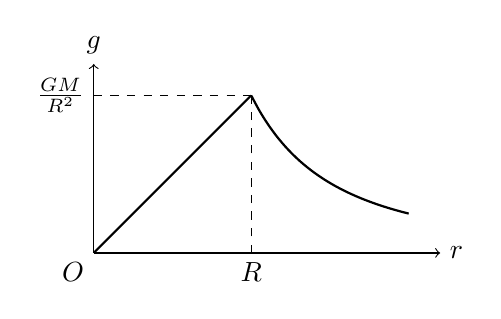
\begin{tikzpicture}[scale=2]
                \draw[->] (0,0) -- (2.2,0) node[right] {$r$};
                \draw[->] (0,0) -- (0,1.2) node[above] {$g$};

                \draw[dashed] (1,0) -- (1,1);
                \draw[dashed] (0,1) -- (1,1);

                \node at (0,0) [below left] {$O$};
                \node at (0,1) [left] {$\frac{GM}{R^2}$};
                \node at (1,0) [below] {$R$};

                \draw[domain=0:1,samples=20,smooth,thick,black]
                plot (\x,\x);
                \draw[domain=1:2,samples=20,smooth,thick,black]
                plot (\x,1/\x^2);
                \end{tikzpicture}
            \end{center}
        }

        \note 推荐一个好用的在线画函数图像网站:\href{https://www.desmos.com/calculator}{www.desmos.com/calculator}。

        \item 判断$g(r)$是否可导。
        
        \sol{
            利用初等函数导数结果可知$g(r)$在$R$以外的点可导,$r$处左导数为$\frac{GM}{R^3}$,右导数为$-\frac{2GM}{R^3}$,它们不相等,因此不可导。
        }

        \note 注意\textbf{不要混淆左/右导数与导数的左/右极限}。导数存在当且仅当左右导数存在且相等,这是由函数极限定义决定的,而导数的左右极限性质我们尚未学到。
    \end{enumerate}

    \item (习题2.1.10)若函数$f(x)$在区间$(-a,a)$上可导,且为偶函数,证明$f'(0)=0$。
    
    \sol{
        \note 事实上利用复合函数导数结论可以直接得到结果,出于课程顺序,这里我们通过\textbf{定义}说明。

        由条件可知
        $$f'(0)=\lim_{x\to0}\frac{f(x)-f(0)}{x}$$
        将$x$换元为$-x$可得
        $$f'(0)=\lim_{x\to0}\frac{f(-x)-f(0)}{-x}=\lim_{x\to0}\frac{f(0)-f(-x)}{x}$$
        两式相加并利用偶函数即得
        $$2f'(0)=\lim_{x\to0}\frac{f(x)-f(-x)}{x}=\lim_{x\to0}\frac{0}{x}=0$$
        这就得到了证明。
    }

    \item (习题2.1.13)求函数
    $$f(x)=\begin{cases}\frac{x}{1+\er^{1/x}}&x\ne0\\0&x=0\end{cases}$$
    在$x=0$处的左右导数。

    \sol{
        由于$x\to0^+$时$\frac{1}{x}\to+\infty$,利用推广的复合函数极限结论可知$\er^{1/x}\to+\infty$,可知\textbf{右导数}为($x$与除以$x$抵消)
        $$\lim_{x\to0^+}\frac{1}{1+\er^{1/x}}=0$$
        同理,由于$x\to0^-$时$\frac{1}{x}\to-\infty$可知$\er^{1/x}\to0$,从而\textbf{左导数}为
        $$\lim_{x\to0^-}\frac{1}{1+\er^{1/x}}=1$$
    }

    \note 应当记忆\textbf{基本初等函数在无穷处的极限情况}。

    \item (2.2节例11)求函数$y=x^x$的导数,其中$x>0$。
    
    \sol{
        由于$x>0$时$x^x=\er^{x\ln x}$,直接利用复合函数求导公式计算可知$x>0$时
        $$y'=(x\ln x)'\er^{x\ln x}=(\ln x+1)\er^{x\ln x}=(\ln x+1)x^x$$
    }

    \item (2.2节例12)求函数
    $$y=\sqrt[3]{\frac{(x+1)^2(2-x)}{(3-x)^2(x-4)}}$$
    的导数。

    \sol{
        此函数在$x\notin\{3,4\}$有定义,由于其为乘积形式,可考虑取绝对值后加$\ln$得到
        $$\ln|y|=\bigg|\sqrt[3]{\frac{(x+1)^2(2-x)}{(3-x)^2(x-4)}}\bigg|$$
        注意$(\ln|x|)'=\frac{1}{x}$对一切$x\ne0$成立,当$y$有定义且非零时(也即$x\notin\{-1,2,3,4\}$)即有
        $$\frac{y'}{y}=\frac{1}{3}\bigg(\frac{2}{x+1}-\frac{1}{2-x}+\frac{2}{3-x}-\frac{1}{x-4}\bigg)$$
        从而
        $$y'=\frac{y}{3}\bigg(\frac{2}{x+1}-\frac{1}{2-x}+\frac{2}{3-x}-\frac{1}{x-4}\bigg)$$

        \note 与之前类似,这类题目无需讨论$x$为$-1$或2时导数的存在性问题,事实上可以\textbf{证明}此时导数不存在:以$x=2$为例,由于$y$在2处为0,导数定义为
        $$\lim_{h\to0}\frac{y(2+h)-0}{h}=\lim_{h\to0}\frac{1}{h}\sqrt[3]{\frac{(h+3)^2(-h)}{(1-h)^2(-2+h)}}$$
        可发现其为
        $$\lim_{h\to0}\frac{y(2+h)-0}{h}=\lim_{h\to0}h^{-2/3}\sqrt[3]{\frac{(h+3)^2}{(1-h)^2(2-h)}}$$
        由于$h^{-2/3}$在0处极限为无穷,右侧部分在0处极限为$\sqrt[3]{9/2}\ne0$,利用无穷极限组合的结论即得此极限为$\infty$,即导数不存在。
    }

    \item (习题2.2.3)计算导数:
    \begin{enumerate}
        \item[(8)] $y=\cos\sqrt[5]{1+x^2}$
        
        \sol{
            利用复合函数求导公式可知
            $$y'=-\frac{2}{5}x(1+x^2)^{-4/5}\sin\sqrt[5]{1+x^2}$$
        }

        \item[(9)] $y=\ln\big|\tan\big(\frac{x}{2}+\frac{\pi}{2}\big)\big|$
        
        \sol{
            利用复合函数求导公式可知
            $$y'=\frac{1}{2}\frac{1}{\tan\big(\frac{x}{2}+\frac{\pi}{4}\big)}\frac{1}{\cos^2\big(\frac{x}{2}+\frac{\pi}{4}\big)}=\frac{1}{2\sin\big(\frac{x}{2}+\frac{\pi}{4}\big)\cos\big(\frac{x}{2}+\frac{\pi}{4}\big)}=\frac{1}{\sin\big(x+\frac{\pi}{2}\big)}=\frac{1}{\cos x}$$
        }
    \end{enumerate}

    \note 直接计算导数类题目一般\textbf{无需讨论定义域}。

    \item (习题2.2.4)计算导数:
    \begin{enumerate}
        \item[(5)] $y=\frac{x}{2}\sqrt{a^2-x^2}+\frac{a^2}{2}\arcsin\frac{x}{a}$,其中$a>0$。
        
        \sol{
            直接计算可知
            $$y'=\frac{1}{2}\sqrt{a^2-x^2}-\frac{x^2}{2\sqrt{a^2-x^2}}+\frac{a^2}{2\sqrt{a^2-x^2}}$$
            后两项合并即发现可进一步化简为
            $$y'=\sqrt{a^2-x^2}$$
        }

        \item[(6)] $y=\frac{x}{2}\sqrt{a^2+x^2}+\frac{a^2}{2}\ln\frac{x+\sqrt{a^2+x^2}}{a}$,其中$a>0$。
        
        \sol{
            直接计算可知(第三项的计算过程相对复杂)
            $$y'=\frac{1}{2}\sqrt{a^2+x^2}+\frac{x^2}{2\sqrt{a^2+x^2}}+\frac{a^2}{2\sqrt{a^2+x^2}}$$
            后两项合并即发现可进一步化简为
            $$y'=\sqrt{a^2+x^2}$$
        }

        \item[(8)] $y=\frac{2}{\sqrt{a^2-b^2}}\arctan\big(\sqrt{\frac{a-b}{a+b}}\tan\frac{x}{2}\big)$,其中$a>b\ge0$。
        
        \sol{
            直接计算可知
            $$y'=\frac{2}{\sqrt{a^2-b^2}}\bigg(1+\frac{a-b}{a+b}\tan^2\frac{x}{2}\bigg)^{-1}\sqrt{\frac{a-b}{a+b}}\frac{1}{\cos^2\frac{x}{2}}\frac{1}{2}$$
            进一步化简可得到
            $$y'=\frac{1}{(a+b)\cos^2\frac{x}{2}+(a-b)\sin^2\frac{x}{2}}$$
            由此展开后再利用二倍角公式得到
            $$y'=\frac{1}{a+b\cos x}$$
        }
    \end{enumerate}

    \item (习题2.2.6)如图所示:
        \begin{center}  
            \begin{tikzpicture}[scale=1]
            \draw (6,0) circle(1);
            \fill (6,0) circle(1pt);
            \node at (6,0) [below right] {$O$};
            \draw[-] (6,0) -- (5.5,0.866);
            \fill (5.5,0.866) circle(1pt);
            \node at (5.5, 0.866) [above left] {$P$};
            \draw[-] (6,0) -- (0,0);
            \fill (3.255,0) circle(1pt);
            \node at (3.255, 0) [below] {$A$};
            \draw[-] (3.255,0) -- (5.5,0.866);
            \end{tikzpicture}
        \end{center}
    圆的半径$OP$为2m,点$P$在圆上顺时针旋转,带动点$A$在水平线上运动,且长度$PA$固定为6m。已知$P$每秒顺时针旋转四圈,求角$AOP$为$\frac{\pi}{2}$且$P$在水平线上方时,点$A$向右运动的瞬时速度。

    \sol{
        以下省略长度单位m与时间单位s。
    
        设$OA$长度为$x$,角$AOP$为$\alpha$\ (这里角度指$AO$\textbf{顺时针}旋转到$OP$所过的角度),它们都是$t$的函数,利用余弦定理可知
        $$36=4+x^2(t)-4x(t)\cos\alpha(t)$$
        两侧同时对$t$求导可知
        $$2x'(t)x(t)-4x'(t)\cos\alpha(t)+4\alpha'(t)x(t)\sin\alpha(t)=0$$
        假设$t_0$时$\alpha(t_0)=\frac{\pi}{2}$,代入可发现
        $$2x'(t_0)x(t_0)+4\alpha'(t_0)x(t_0)=0$$
        由几何关系$x(t_0)\ne0$,消去可得
        $$x'(t_0)=-2\alpha'(t_0)$$
        利用条件,由于$P$在顺时针旋转,$\alpha'(t_0)$为正,且根据条件可知角速度恒定为$8\pi$,因此即得
        $$x'(t_0)=-16\pi$$
        注意这意味着$OA$瞬时以$16\pi$\,m/s的速度缩短,对应点$A$向右运动,于是$A$向右运动的顺时速度为$16\pi$\,m/s。
    
    }
    
    \item (习题2.5.1)判断$x\to0$时以下无穷小量关于$x$的阶数:
    \begin{enumerate}[(1)]
        \item $y=x+10x^2+100x^3$
        
        \sol{
            由于$x\to0$时$x^2$与$x^3$衰减将更快,可\textbf{感受}出$y$是$x$的一阶无穷小,由此尝试证明:
            $$\lim_{x\to0}\frac{y}{x}=\lim_{x\to0}(1+10x+100x^2)=1$$
            从而的确为一阶无穷小。
        }

        \item $y=(\sqrt{x+2}-\sqrt{2})\sin x$
        
        \sol{
            由基本等价无穷小结论$x\to0$时$\sin x\sim x$,$(\sqrt{x+1}-x)\sim\frac{1}{2}x$,可\textbf{感受}出$y$是$x$的二阶无穷小,由此尝试证明
            $$\lim_{x\to0}\frac{y}{x^2}=\lim_{x\to0}\frac{\sqrt{2}\big(\sqrt{\frac{x}{2}+1}-1\big)}{x}\frac{\sin x}{x}$$
            利用等价无穷小替换可知上方分子上的$\sqrt{\frac{x}{2}+1}-1$可替换为$\frac{1}{2}\cdot\frac{x}{2}=\frac{x}{4}$,由此进一步计算得
            $$\lim_{x\to0}\frac{y}{x^2}=\frac{\sqrt2}{4}$$
            从而的确为二阶无穷小。
        }

        \note 注意$\sqrt{x+c}-\sqrt{c}$在$c\ne0$时是\textbf{一阶}无穷小,否则其为$\sqrt{x}$,是$\frac{1}{2}$阶无穷小。

        \item $y=x(1-\cos x)$
        
        \sol{
            有基本等价无穷小结论$x\to0$时$(1-\cos x)\sim\frac{1}{2}x^2$,从而直接有
            $$\lim_{x\to0}\frac{y}{x^3}=\lim_{x\to0}\frac{1-\cos x}{x^2}=\frac{1}{2}$$
            由此$y$为$x$的三阶无穷小。
        }
    \end{enumerate}

    \note 未知阶数时需要先分析\textbf{估算出阶数},若证明过程中发现有问题再调整。

    \item (习题2.5.8(3))求以下方程确定的隐函数$y(x)$的导数:
    $$\arctan\frac{y}{x}=\ln\sqrt{x^2+y^2}$$

    \sol{
        两侧对$x$求导可发现
        $$\frac{1}{(y/x)^2+1}\frac{xy'-y}{x^2}=\frac{x+yy'}{x^2+y^2}$$
        注意两边分母相同,且由原式有$\ln\sqrt{x^2+y^2}$可知$x^2+y^2\ne0$,消去分母即得到($x\ne y$时)
        $$y'=\frac{x+y}{x-y}$$
    }

    \note 求导时务必注意\textbf{不要忘记$y$是$x$的函数}。此外,这类题目无需进一步讨论$x=y$时的可导性。

    \item (习题2.5.9(2))求以下方程确定的隐函数在$\big(\frac{\er}{10},\frac{20}{\er^2}\big)$的导数:
    $$\er^{xy}-5x^2y=0$$

    \sol{
        两侧对$x$求导可发现
        $$(y+xy')\er^{xy}-5x^2y'-10xy=0$$
        由条件$\er^{xy}=5x^2y$代入并消去$5x$可进一步化简为
        $$xy^2+x^2yy'-xy'-2y=0$$
        也即($x^2y-x\ne0$时)
        $$y'=\frac{2y-xy^2}{x^2y-x}$$
        代入即可得到这点处导数为0。
    }

    \item (习题2.5.10(2))计算以下参数方程确定的函数$y(x)$的导数:
    $$\begin{cases}x=t\ln t\\y=\er^t\end{cases}$$
    
    \sol{
        代入公式(推导可见本讲义5.3.2)可得导数为($1+\ln t\ne0$时)
        $$y'(x)=\frac{\frac{\dr y}{\dr t}}{\frac{\dr x}{\dr t}}=\frac{\er^t}{1+\ln t}$$
    }

    \item (习题2.5.11)求椭圆周
    $$\frac{x^2}{a^2}+\frac{y^2}{b^2}=1,\quad a>0,b>0$$
    上一点$M(x_0,y_0)$处的切线方程与法线方程。证明从一个焦点出发射向$M$的光线将通过另一个焦点。

    \sol{
        椭圆方程两侧对$x$求导可得
        $$\frac{2x}{a^2}+\frac{2yy'}{b^2}=0$$
        从而可知
        $$y'=-\frac{b^2x}{a^2y}$$
        由此可知$M$处的切线斜率为$-\frac{b^2x_0}{a^2y_0}$,由斜率乘积为$-1$的直线垂直可知法线斜率为$\frac{a^2y_0}{b^2x_0}$,从而切线、法线方程分别为(虽然上述推导中默认了$x_0$、$y_0$非零,单独讨论可以发现当其中某个为0时下方也仍然为切线或法线的方程)
        $$a^2y_0(y-y_0)+b^2x_0(x-x_0)=0$$
        $$b^2x_0(y-y_0)-a^2y_0(x-x_0)=0$$
        接下来证明反射性质。

        不妨设$a>b>0$,记$c=\sqrt{a^2-b^2}$,则焦点为
        $$F_1(-c,0),\quad F_2(c,0)$$
        向量$F_1M$、$F_2M$分别为
        $$\alpha=(x_0+c,y_0),\quad\beta=(x_0-c,y_0)$$
        任取法线上两点(如$(x_0,y_0)$与$\big(x_0+b^2x_0,y_0+a^2y_0)$)连线,可得法线的方向向量
        $$\gamma=(b^2x_0,a^2y_0)$$
        要证明$MF_1$、$MF_2$互为反射光线只需证明它们与法线夹角相等,这又等价于夹角$\cos$值相等,利用向量内积的性质可得也即
        $$\frac{\alpha\cdot\gamma}{|\alpha||\gamma|}=\frac{\beta\cdot\gamma}{|\beta||\gamma|}$$
        由点在椭圆上$b^2x_0^2+a^2y_0^2=a^2b^2$,从而
        $$(x_0\pm c,y_0)\cdot\gamma=b^2(a^2\pm cx_0)$$
        由此
        $$\frac{\alpha\cdot\gamma}{\beta\cdot\gamma}=\frac{a^2+cx_0}{a^2-cx_0}$$
        再代入
        $$y_0^2=\frac{a^2b^2-b^2x_0^2}{a^2}=\frac{a^2-x_0^2}{a^2}(a^2-c^2)$$
        可发现
        $$|(x_0\pm c,y_0)|=\sqrt{x_0^2+c^2\pm2cx_0+\frac{a^2-x_0^2}{a^2}(a^2-c^2)}=\frac{1}{a}\sqrt{a^4+c^2x_0^2\pm2cx_0a^2}=\frac{1}{a}|a^2\pm cx_0|$$
        注意由$|x_0|\le a$与$c$的定义有$a^2\pm cx_0>0$即可得证。

    }

    \item (2.6节例6)设$y(x)$是由方程$x^3+y^3-3xy=0$所确定的隐函数,求$y''$。
    
    \sol{
        方程两边同时求导得到
        $$3x^2+3y^2y'-3xy'-3y=0$$
        从而
        $$y'=\frac{y-x^2}{y^2-x}$$
        由此利用复合函数求导再次求导可知
        $$y''=\frac{(y'-2x)(y^2-x)-(2yy'-1)(y-x^2)}{(y^2-x)^2}$$
        代入$y'$得到
        $$y''=\frac{(y-x^2-2x(y^2-x))(y^2-x)-(2y(y-x^2)-(y^2-x))(y-x^2)}{(y^2-x)^3}$$
        分子展开可得
        $$y''=\frac{-2xy^4+6x^2y^2-2yx^4-2xy}{(y^2-x)^3}$$
        注意$-2xy^4+6x^2y^2-2yx^4=-2xy(y^3+x^3-3xy)=0$,从而最终化为
        $$y''=-\frac{2xy}{(y^2-x)^3}$$

        \note 考试的时候一般不会因为化不到最简扣分,但除非时间不够,否则请\textbf{尽量化简}以避免助教看错。
    }

    \item (2.6节例7)设$y(x)$是由参数方程
    $$\begin{cases}x=t-\sin t\\y=1-\cos t\end{cases}$$
    确定的函数,求$y''$。

    \sol{
        代入公式可得
        $$y'=\frac{-\sin t}{1-\cos t}$$
        将此与$x=t-\sin t$组合看作新的参数方程,再次代入公式得到
        $$y''=\bigg(\frac{\sin t}{1-\cos t}\bigg)'\frac{1}{1-\cos t}$$
        直接计算并化简即得到
        $$y''=-\frac{1}{(1-\cos t)^2}$$
    }

    \item (习题2.6.8)设$y=x^2\ln(1+x)$,求$y^{(50)}$。
    
    \sol{
        由于$y$为$x^2$与$\ln(1+x)$的乘积,利用乘积的$n$阶导数公式,由于$x^2$求3阶及以上导数为0即得
        $$y^{(50)}=x^2(\ln(1+x))^{(50)}+50\cdot 2x(\ln(1+x))^{(49)}+\frac{50\cdot49}{2}\cdot 2(\ln(1+x))^{(48)}$$
        直接递推计算可发现$n>1$时
        $$(\ln(1+x))^{(n)}=(-1)^{n-1}(n-1)!\frac{1}{(1+x)^n}$$
        由此可得
        $$y^{(50)}=-49!\frac{x^2}{(1+x)^{50}}+100\cdot48!\frac{x}{(1+x)^{49}}-50\cdot49\cdot47!\frac{1}{(1+x)^{48}}$$
    }
    \item (习题2.7.2)计算
    $$\int(1+\sqrt{x})^2\dr x$$

    \sol{
        展开后利用幂函数导数结论即得
        $$\int(1+2\sqrt{x}+x)\dr x=x+\frac{4}{3}x^{\frac{3}{2}}+\frac{1}{2}x^2+C$$
    }

    \note 不定积分题目同样\textbf{一般无需严格说明定义域},其实际影响本章中将介绍。

    \item (习题2.7.4)计算
    $$\int\tan^2t\dr t$$

    \sol{
        由于$\tan^2t=\frac{\sin^2t}{\cos^2t}$,而我们知道$\tan t$的导数为$\frac{1}{\cos^2t}$,可以想到将原式配凑为
        $$\int(\tan^2t+1-1)\dr t=\int\bigg(\frac{1}{\cos^2t}-1\bigg)\dr t=\tan t-t+C$$
    }

    \note 由以上两题可发现$\int f(x)\dr x$与$\int f(t)\dr t$是\textbf{不同}的,分别是$x$与$t$的函数。

    \item (习题2.7.6)计算
    $$\int\frac{x^2+3}{1+x^2}\dr x$$
    \sol{
        我们优先将分式\textbf{分离出整式部分}得到其为
        $$\int\bigg(1+\frac{2}{1+x^2}\bigg)\dr x=x+2\arctan x+C$$
        
        \note 此方法的原理和更多应用将在介绍有理函数不定积分时介绍。
    }

    \item (习题2.7.8)计算
    $$\int(1+\cos^2x)\sec^2x\dr x$$
    \sol{
        直接展开得到其为
        $$\int\bigg(\frac{1}{\cos^2x}+1\bigg)\dr x=\tan x+x+C$$
    }

    \note 个人建议计算中尽量\textbf{将三角函数优先化为$\sin$与$\cos$},这样可以看出问题的实际形式。

    \item (习题2.7.10)计算
    $$\int\bigg(\frac{1}{x}+\frac{2}{x^2}+\frac{3}{x^3}\bigg)\dr x$$

    \sol{
        直接由幂函数与对数函数导数结论得其为
        $$\ln|x|-\frac{2}{x}-\frac{3}{2x^2}+C$$
    }

    \item (习题2.7.12)计算
    $$\int(2\cosh x-\sinh x)\dr x$$

    \sol{
        直接展开得到其为
        $$\int\bigg(\frac{1}{2}\er^x+\frac{3}{2}\er^{-x}\bigg)\dr x=\frac{1}{2}\er^x-\frac{3}{2}\er^{-x}+C$$
        等号是利用了指数函数导数结论。
    }

    \note 同样,计算中\textbf{双曲函数也优先展开},因为指数函数是易于处理的。

    \item (习题2.7.14)计算
    $$\int\frac{1}{\sin^2x\cos^2x}\dr x$$

    \sol{
        由于分子实际上是$\sin^2x+\cos^2x$,可以将其展开为
        $$\int\bigg(\frac{1}{\sin^2x}+\frac{1}{\cos^2x}\bigg)\dr x$$
        这样即可以通过三角函数导数结论得到结果为
        $$-\cot x+\tan x+C$$
    }

    \item (习题2.7.16)计算
    $$\int\frac{1}{x^2(1+x^2)}\dr x$$
    
    \sol{
        注意到$1+x^2-x^2=1$,由此可以想到裂项得上式为
        $$\int\bigg(\frac{1}{x^2}-\frac{1}{1+x^2}\bigg)\dr x=-\frac{1}{x}-\arctan x+C$$
    }

    \item (习题2.7.18)设$f(x)$在$\rb$中某区间满足微分方程
    $$xf'(x)+f(x)=x^3+1$$
    求所有可能的$f(x)$。

    \sol{
        观察得到左侧为$(xf(x))'=x^3+1$,由此即可得到存在$C\in\rb$使得
        $$xf(x)=x^4+x+C$$
        若此区间不包含0,上式可以直接得到
        $$f(x)=x^3+1+\frac{C}{x}$$
        若包含0,代入$x=0$可知$C\ne0$时无解,从而只能
        $$f(x)=x^3+1$$
    }

    \item (习题2.8.1(2))用定义计算
    $$\int_a^bx\dr x$$

    \sol{
        \note 教材中这类题目直接应用了\textbf{连续函数可积},从而直接取特定分点进行了证明,我们此处给出一个不默认可积的证明方式。

        利用面积的直观感受可以得到结果为$\frac{b^2-a^2}{2}$,下面证明此结果。

        对划分$T\colon a=x_0<x_1<\dots<x_n=b$,由定义得需要考虑以下求和
        $$\sum_{k=1}^n\xi_k(x_k-x_{k-1})$$
        其中$\xi_k\in(x_{k-1},x_k)$。
        为了配凑出$\frac{b^2-a^2}{2}$,我们发现它可以看作裂项求和
        $$\frac{b^2-a^2}{2}=\sum_{k=1}^n\frac{x_k^2-x_{k-1}^2}{2}=\sum_{k=1}^n\frac{x_{k-1}+x_k}{2}(x_k-x_{k-1})$$
        从而有估算
        $$\begin{aligned} &\bigg|\sum_{k=1}^n\xi_k(x_k-x_{k-1})-\frac{b^2-a^2}{2}\bigg|\\=&\bigg|\sum_{k=1}^n\bigg(\xi_k-\frac{x_k+x_{k-1}}{2}\bigg)(x_k-x_{k-1})\bigg|\\\le&\sum_{k=1}^n\bigg|\xi_k-\frac{x_k+x_{k-1}}{2}\bigg|(x_k-x_{k-1})\\\le&\sum_{k=1}^n\frac{x_k-x_{k-1}}{2}(x_k-x_{k-1})\\=&\frac{1}{2}\sum_{k=1}^n(x_k-x_{k-1})^2\end{aligned}$$
        这里最后一个$\le$号是由于$\xi_k$的范围限制。

        设$\lambda(T)$为$T$最长分段的长度,则对任何$k$有$(x_k-x_{k-1})^2\le\lambda(T)(x_k-x_{k-1})$,从而进一步放缩得到
        $$\bigg|\sum_{k=1}^n\xi_k(x_k-x_{k-1})-\frac{b^2-a^2}{2}\bigg|\le\frac{1}{2}\sum_{k=1}^n(x_k-x_{k-1})^2\le\frac{1}{2}\lambda(T)\sum_{k=1}^n(x_k-x_{k-1})=\frac{b-a}{2}\lambda(T)$$
        由此即可以利用定积分定义证明$\lambda(T)$趋于0时左侧极限为0,得证。
    }

    \item (习题2.8.6)判断下列各题中定积分值的大小:
    \begin{enumerate}[(1)]
        \item $\int_0^1\er^x\dr x$与$\int_0^1\er^{x^2}\dr x$
        
        \sol{
            左减右得
            $$\int_0^1(\er^x-\er^{x^2})\dr x=\int_0^1\er^x(1-\er^{x^2-x})\dr x$$
            由$(0,1)$上$x^2-x<0$可知上式被积函数在$(0,1)$恒正,又由连续且恒正可知积分大于0,从而左大于右。
        }

        \item $\int_0^{\pi/2}x^2\dr x$与$\int_0^{\pi/2}\sin^2x\dr x$
        
        \sol{
            左减右得
            $$\int_0^{\pi/2}(x^2-\sin^2x)\dr x$$
            由三角函数估算结论$x>0$时$x>\sin x$可知上式被积函数在$(0,\frac{\pi}{2})$恒正,又由连续且恒正可知积分大于0,从而左大于右。
        }

        \item $\int_0^1x\dr x$与$\int_0^1\sqrt{1+x^2}\dr x$
        
        \sol{
            左减右得
            $$\int_0^1(x-\sqrt{1+x^2})\dr x$$
            由$(0,1)$上$x<1<\sqrt{1+x^2}$可知上式被积函数在$(0,1)$恒负,又由连续且恒负可知积分小于0,从而左小于右。
        }

    \end{enumerate}
    \note 注意从开区间恒正推出积分值为正的过程\textbf{需要被积函数连续}。虽然教材未对此进行说明,本章\exref{cont nonneg int}将介绍证明过程。
\end{enumerate}

\subsection{积分}
\subsubsection{不定积分定义}
首先,给定函数可以计算导函数,那么,给定某开区间(可能含无穷)上的函数$f(x)$,我们自然也希望能求解出\textbf{原函数},也即满足$F'(x)=f(x)$处处成立的函数$F$。

为了说明原函数的性质,我们需要如下的关键定理:
\begin{framed}
\begin{exercise}\label{deri const}
    若函数$f(x)$在某开区间(可能含无穷)上可导且$f'(x)$恒为0,证明$f(x)$为常数。

    \note 此结论的逆命题即开区间\textbf{常函数导数为0},可由导数定义直接得到,从而成立。
\end{exercise}
\sol{
    我们会自然想到反证的思路:若此区间中有$a<b$使得$f(a)\ne f(b)$,我们希望证明$[a,b]$中有一点使得$f'(x)\ne0$。

    截至目前,我们学过的唯一一个函数值和导数相关的结论是高中时期的\textbf{函数极值点导数为0},接下来我们先用导数的严谨性证明此结论,再利用它做出本题:

    \begin{itemize}
        \item \textbf{极值点性质}
        
        若存在$\delta>0$使得只要$|x-x_0|<\delta$就有$f(x)\le f(x_0)$,则称$x_0$为$f$的\textbf{极大值点},我们将证明,若$f$在$x_0$可导,则$f'(x_0)=0$。

        若$f'(x_0)>0$,利用极限保序性可知存在$\delta_0>0$使得
        $$\forall0<|h|<\delta_0,\quad\frac{f(x_0+h)-f(x_0)}{h}>0$$
        由此对任何$h\in(0,\delta_0)$都有$f(x_0+h)>f(x_0)$,与极大值定义矛盾。

        反之,若$f'(x_0)<0$,利用极限保序性可知存在$\delta_0>0$使得
        $$\forall0<|h|<\delta_0,\quad\frac{f(x_0+h)-f(x_0)}{h}<0$$
        由此对任何$h\in(-\delta_0,0)$都有$f(x_0+h)>f(x_0)$,与极大值定义矛盾。

        \note 同理可定义\textbf{极小值点},并证明极小值点若可导则导数为0。

        \item \textbf{函数构造}
        
        \note 这步的过程有一定技巧性,可以学习思想。

        用刚才证明的结论可以找到导数为0的点,但我们的反证法需要构造$f'(x)$不为0的点,由此可以想到利用\textbf{差的导数是导数的差},只要我们构造另一个\textbf{导数不为0}的函数$g(x)$,使得$f(x)-g(x)$在某点导数为0,就可以得到$f(x)$在这点的导数非零0。

        由此,我们考虑最简单的导数非零的函数,\textbf{一次函数},记
        $$g(x)=\frac{f(b)-f(a)}{b-a}x+\frac{bf(a)-af(b)}{b-a}$$
        可发现由条件$g'(x)=\frac{f(b)-f(a)}{b-a}\ne0$,且$g(a)=f(a)$、$g(b)=f(b)$。

        我们记$h(x)=f(x)-g(x)$,则$h(a)=h(b)=0$。我们下面证明存在$x_0\in(a,b)$使得$h'(x_0)=0$,则有
        $$f'(x_0)=g'(x_0)=\frac{f(b)-f(a)}{b-a}\ne0$$
        这样就得到了矛盾。

        \item \textbf{最终证明}

        考虑区间$[a,b]$,由于$f$、$g$都是连续函数($f$可导于是连续),$h$在$[a,b]$上连续,由此利用连续函数最值性质(可见\exref{max min}),$h$在$[a,b]$上存在最大值$M$与最小值$m$。利用条件有$h(a)=h(b)=0$,于是$M\ge 0\ge m$。

        若$M=m=0$,$h$在$[a,b]$上恒为0,任取$x_0\in(a,b)$均符合要求。否则,不妨设$M>0$\ ($m<0$同理),假设$h$在$x_0$处取到最大值$M$,利用两端为0可知$x_0\in(a,b)$。记$\delta=\min(x_0-a,b-x_0)$,即可由极大值点定义发现$x_0$是$h$的极大值点,从而$h'(x_0)=0$,得证。

        \note 这里最后一段证明了闭区间中不在两端的\textbf{最值点}若可导则一定导数为0。从几何直观可以感受到最值点一定是极值点,因此结论是自然的。
        
    \end{itemize}

    \note 我们实质上证明了,对任何$[a,b]$上连续、$(a,b)$上可导的函数$f$,存在$\xi\in(a,b)$使得$f'(\xi)=\frac{f(b)-f(a)}{b-a}$,这是\textbf{微分中值定理}的重要形式。
}
\end{framed}

有了此定理后,我们可以马上得到结论:给定某开区间(可能含无穷),若$f(x)$在其上的一个原函数为$F(x)$,则全部原函数为
$$\{F(x)+C\mid C\in\rb\}$$
这是由于$G(x)$是$f(x)$的原函数\textbf{当且仅当}$(G(x)-F(x))'=0$。

\note 或许有的同学会注意到,此结论与证明方式和线性代数上``非齐次线性方程组的通解是对应齐次线性方程组通解加原方程组特解''非常类似。事实上在学到线性空间与线性映射后可以发现这两个结论\textbf{本质是相同的}。

\

不过,对于一般情况,原函数可能会更加复杂,也可能并不存在,我们以下面两个例子进行介绍:
\begin{framed}
\begin{exercise}
    求所有定义在$(-\infty,0)\cup(0,+\infty)$的函数$f(x)$使得$f'(x)=\frac{1}{x}$。
\end{exercise}
\sol{
    直接计算导数可以发现
    $$(\ln x)'=\frac{1}{x}$$
    $$(\ln(-x))'=\frac{1}{x}$$
    从而再考虑定义域可知$f(x)=\ln|x|$满足要求。对于$(-\infty,0)$与$(0,+\infty)$分别使用区间上的原函数结论可知满足条件的所有$f(x)$可以写成
    $$f(x)=\begin{cases}\ln(-x)+C_1&x<0\\\ln x+C_2&x>0\end{cases}$$
    的形式,其中$C_1$、$C_2$为任意常数。

    \note 由于定义域的中断,无需$C_1=C_2$,可以直接计算验证上述$f(x)$都符合要求。
}
\end{framed}
从这个例子中可以看出,若$f(x)$的定义域是不同的区间拼接而成的,导数为$f(x)$的函数$F(x)$应可以\textbf{在每个区间加不同的任意常数$C$}。

\note 此时我们仍然将导数为$f(x)$的函数$F(x)$称为$f(x)$的原函数。

\begin{framed}
\begin{exercise}\label{no ori func}
    证明不存在$\rb$上的函数$F(x)$使得$F'(x)=f(x)$,其中
    $$f(x)=\begin{cases}0&x\ne0\\1&x=0\end{cases}$$
\end{exercise}
\sol{
    假设存在,由于$F(x)$在$(-\infty,0)$上导数为0,由\exref{deri const}可知其在$(-\infty,0)$上为常数,同理其在$(0,+\infty)$上为常数,从而
    $$F(x)=\begin{cases}C_1&x<0\\C_2&x=0\\C_3&x>0\end{cases}$$
    由于$F(x)$在0处可导,其必然连续,利用定义可知$C_1=C_2=C_3$,这样即可得到$F(x)$为常函数,从而$F'(0)=0$,与$f(0)=1$矛盾。
}
\end{framed}

这个例子也可以推广:若$f(x)$在某开区间(可能含无穷)上存在原函数,我们可以证明改变$f(x)$某点的值后其一定不存在原函数。

\note 假设$f(x)$的一个原函数为$F(x)$,$f(x)$改变某点值后为$g(x)$,若$g(x)$有原函数$G(x)$,根据定义$(F(x)-G(x))'$在区间内只有一点非零,其他点均为0,与上方例子同理证得矛盾。

\

至此,我们可以给出\textbf{原函数}的严谨定义:任给函数$f(x)$,假设$f(x)$的定义域为$E$,我们将$E$中所有\textbf{有邻域的点}(即存在$\delta$使得$(x_0-\delta,x_0+\delta)\in E$)的集合记为$E^\circ$。若定义在$E^\circ$上的$F(x)$满足对$E^\circ$任何点都有$F'(x)=f(x)$,则称$F(x)$为$f(x)$的一个原函数。

补充一些注释:
\begin{itemize}
    \item 当$E=[a,b]$时,利用定义可发现$E^\circ=(a,b)$,由此闭区间的原函数\textbf{无需考虑端点处}。例如,$f(x)=\sqrt{x}$的定义域为$[0,+\infty)$,当我们在说$F(x)=\frac{2}{3}x^{3/2}$是$f(x)$的原函数时,我们只考虑了$(0,+\infty)$上每一点$F(x)$的导数。
    
    \item 一般情况下不定积分题目无需特别考虑定义域问题,只要\textbf{形式上求导得到的结果符合},我们就可以认为是一个原函数。
    
    \item 务必记住\textbf{所有基本初等函数的导数},它们是最基本的反推原函数的方式(称为\textbf{基本积分表})。
\end{itemize}

\

不过,有了原函数后,我们尚未解决不定积分的定义问题。直觉的不定积分定义是,若$F(x)$是$f(x)$的一个原函数,$F(x)+C$应为所有原函数(这里$C$为任意常数),从而可记
$$\int f(x)\dr x=F(x)+C$$

但是,此定义有三个奇怪之处:
\begin{enumerate}
    \item 这里的$C$代表的``任意常数'',似乎与普通的常数不同,因为根据定义
    $$\int x\dr x=\frac{1}{2}x^2+C,\quad\int x\dr x=\frac{1}{2}x^2+1+C$$
    都是正确的。但是,联立两式可以得到$\frac{1}{2}x^2+C=\frac{1}{2}x^2+1+C$,这又貌似是错误的。我们当然希望\textbf{等式是可以联立的},因此上述过程必然有什么地方出了问题。

    \item $C$还有另一个奇怪之处,根据不定积分定义可以写出
    $$\int\frac{\dr x}{x}=\ln|x|+C$$
    但是我们已经知道$\frac{1}{x}$的全部原函数为
    $$\begin{cases}\ln(-x)+C_1&x<0\\\ln x+C_2&x>0\end{cases}$$
    若我们真的希望$\ln|x|+C$是$\frac{1}{x}$的全部原函数,此处一个$C$需要表示两个不同的任意常数。

    \item 此外,如果我们将$F$作为$f$的\textbf{原函数}进行理解,那么$f(x)=\frac{x^2}{2}$与$f(t)=\frac{t^2}{2}$应当表示\textbf{同一个函数}(即使将$t$换为$2x$整体也不影响),由此通过
    $$\int t\dr t=\frac{t^2}{2}+C$$
    $$\int x\dr x=\frac{x^2}{2}+C$$
    可知右侧应当相等,但由于右侧$x$、$t$都是任意的,我们可以任取,如取$t=2x$时右侧自然并不相等。
\end{enumerate}

虽然上述问题看起来有点``无理取闹'',但对理解不定积分来说又是必要的。否则,我们将难以理解一些更加复杂的计算过程(如教材3.2节例8得到的关于不定积分的``方程式'')。

我们现在来通过严谨定义一步步解决这三个问题:
\begin{itemize}
    \item 首先,对第三个问题,我们必须注意不定积分的结果\textbf{不是函数而是表达式}。
    
    何为表达式?最简单的例子是,$f(x)=x$与$f(t)=t$代表同一个函数(只要定义域相同,这两个函数都表示把每一点映射到自身),但$x$与$t$是两个\textbf{不同}的表达式。事实上,$f(x)=x$是\textbf{用表达式定义了函数},而不定积分
    $$\int f(x)\dr x,\quad\int f(t)\dr t$$
    的结果分别是含$x$、含$t$的\textbf{表达式},因此不同。

    在不会引起歧义时,我们往往并不区分函数和表达式,例如我们会允许$(\sin x)'=\cos x$这样的式子。虽然严谨来说我们只能写
    $$\frac{\dr}{\dr x}\sin x=\cos x$$
    或
    $$f(x)=\sin x,\quad f'(x)=\cos x$$
    但当表达式里的变量唯一时,我们默认$(f(x))'$表示$\frac{\dr}{\dr x}f(x)$。

    更进一步地,$f'(x)$事实上指的是,将对$f$求导形成的新的函数\textbf{代入}$x$后形成的表达式。由此,当我们写下
    $$\frac{\dr}{\dr x}\sin x=\cos x$$
    时,实际上进行了三个步骤:
    \begin{enumerate}
        \item 定义函数$f(x)=\sin x$;
        \item 计算函数$f$的导函数$f'$,它满足$f'(t)=\cos t$;
        \item 在$f'$里代入$x$形成新的表达式$\cos x$,以此作为结果。
    \end{enumerate}

    这样就可以解释不定积分了,例如
    $$\int x\dr x=\frac{x^2}{2}+C$$
    表示类似的三个步骤:
    \begin{enumerate}
        \item 定义函数$f(x)=x$;
        \item 计算函数$f$的一个原函数$F$,它满足$F(t)=\frac{t^2}{2}$;
        \item 在$F$里代入$x$形成新的表达式$\frac{x^2}{2}$,以$\frac{x^2}{2}+C$作为结果。
    \end{enumerate}

    一句话总结上述过程:\textbf{对某个变量$a$进行不定积分得到的是含$a$的表达式},将表达式中的变量替换会得到不同表达式,由此$\int f(x)\dr x\ne\int f(t)\dr t$。

    \item 对于第一个问题,它的解决方案本质是\textbf{线性代数}知识(也即商空间中的元素),我们这里以当前能理解的方式进行介绍。
    
    以定义在$\rb$上的函数$f(x)$为例,我们认为不定积分
    $$\int f(x)\dr x$$
    的结果并不是一个元素,而是一个\textbf{表达式集合}:
    $$\{F(x)+C\mid C\in\rb\}$$
    由此,$F(x)+C$事实上是$\{F(x)+C\mid C\in\rb\}$的简写。这样,我们就的确可以自信地写出
    $$F(x)+C=F(x)+1+C$$
    了,因为
    $$\{F(x)+C\mid C\in\rb\}=\{F(x)+C+1\mid C\in\rb\}$$

    \note 证明是简单的,左边的每个$F(x)+C$都可以对应右边的$F(x)+(C-1)+1$,因此左包含于右,同理右包含于左。

    由此,这里的$+C$实际上是\textbf{表达集合的形式记号},当我们写$+C$时默认其表示集合,这就是``任意常数''的含义。

    \item 对于第二个问题,既然$+C$只是一个形式记号,它所表达的集合当然可以不止是$F(x)+C$,例如,在我们写出
    $$\int\frac{1}{x}\dr x=\ln|x|+C$$
    时,有
    $$\ln|x|+C=\left\{f(x)\mid f(x)=\begin{cases}\ln x+C_1&x>0\\\ln(-x)+C_2&x<0\end{cases},\quad C_1,C_2\in\rb\right\}$$

    由此,当$f(x)$定义域有多个区间时,$F(x)+C$事实上表示\textbf{$F(x)$每个区间加一个不同实数所能构成的所有表达式的集合}。

    \item 解决这三个问题后,为了使以下符合直觉的的运算法则成立(下方$c$为实数):
    $$\int(f(x)+g(x))\dr x=\int f(x)\dr x+\int g(x)\dr x,\quad c\int f(x)\dr x=\int cf(x)\dr x$$
    我们还需要定义\textbf{表达式集合的运算}。假设$A$、$B$为表达式集合,$r$为某表达式,我们定义运算如下(这些定义还是相对\textbf{符合直觉}的,大家可以在下面的过程里进行感受):
    $$r+A=A+r=\{a+r\mid a\in A\}$$
    $$A+B=\{a+b\mid a\in A,b\in B\}$$
    $$rA=\{ra\mid a\in A\}$$
    由此即可证明上方的运算律。
    
    \note 我们以第一式为例,简单起见设$f(x)$、$g(x)$定义域为$\rb$。假设$f(x)$的一个原函数为$F(x)$、$g(x)$的一个原函数为$G(x)$,可发现$f(x)+g(x)$的一个原函数为$F(x)+G(x)$,由此只需证明
    $$F(x)+G(x)+C=(F(x)+C)+(G(x)+C)$$
    利用定义此即代表
    $$\{F(x)+G(x)+C\mid C\in\rb\}=\{F(x)+C\mid C\in\rb\}+\{G(x)+C\mid C\in\rb\}$$
    利用定义展开右侧,由于第一个集合中某元素是$F(x)+C_1$、第二个集合中某个元素是$G(x)+C_2$,上式等价于
    $$\{F(x)+G(x)+C\mid C\in\rb\}=\{F(x)+C_1+G(x)+C_2\mid C_1, C_2\in\rb\}$$
    左边的每个元素都可以在右侧令$C_1=C$、$C_2=0$得到,从而左包含于右;右边的每个元素都可以在左侧令$C=C_1+C_2$得到,从而右包含于左。这样就得到了证明。
\end{itemize}

正如之前所说,不定积分相关的大部分严谨性问题我们都可以通过\textbf{直觉}来解决,但这些严谨定义对于理解复杂过程是必要的。现在,大家可以严谨证明为何教材3.2节例8得到的方程式
$$J=\int\er^{ax}\cos(bx)\dr x$$
$$J=\bigg(\frac{1}{a}\cos(bx)+\frac{b}{a^2}\sin(bx)\bigg)\er^{ax}-\frac{b^2}{a^2}J$$
的解只有
$$J=\frac{1}{a^2+b^2}(a\cos(bx)+b\sin(bx))\er^{ax}+C$$
了。

\note 注意不能对方程直接移项,因为本来左右都是集合,将$-\frac{b^2}{a^2}J$移到左侧会形成``集合与数相等''的形式,这是荒谬的。

\begin{framed}
\begin{exercise}[\extra]\label{inte equa}
    考虑定义在$\rb$上的函数$g$,其存在原函数。若
    $$J=\int g(x)\dr x$$
    且存在不相等的实数$a$、$b$与$\rb$上的函数$F$使得
    $$aJ=F(x)+bJ$$
    证明
    $$J=\frac{1}{a-b}F(x)+C$$
\end{exercise}
\sol{
    设$g$的一个原函数为$G(x)$,则$J=G(x)+C$,利用表达式集合的运算定义可发现方程变为
    $$\{aG(x)+aC\mid C\in\rb\}=\{F(x)+bG(x)+bC\mid C\in\rb\}$$
    由两集合相等可知左侧包含于右侧,也即
    $$\forall C_1\in\rb,\quad\exists C_2\in\rb,\quad aG(x)+aC_1=F(x)+bG(x)+bC_2$$
    将其重新写为
    $$\forall C_1\in\rb,\quad\exists C_2\in\rb,\quad G(x)=\frac{1}{a-b}F(x)+\frac{bC_2-aC_1}{a-b}$$
    取定$C_1=0$,取出此时的$C_2$,由于$\frac{bC_2}{a-b}$为实数,可知存在$C_0\in\rb$使得
    $$G(x)=\frac{1}{a-b}F(x)+C_0$$
    与之前类似通过两方面包含可验证此时$J=G(x)+C$的确满足
    $$aJ=F(x)+bJ$$
    从而有(加实数$C_0$不影响任意常数,这已经在之前讨论中证明)
    $$J=\frac{1}{a-b}F(x)+C_0+C=\frac{1}{a-b}F(x)+C$$
}
\end{framed}

\note 注意我们上述的所有推导都是以$g(x)$\textbf{存在原函数}为前提,由此教材3.2节例8得到$J$的形式后必须\textbf{求导验证}其确为原函数才能成立,教材漏掉了这一步。

\subsubsection{定积分定义}
对于定积分,我们需要先定义划分:我们将满足$a=x_0<x_1<\dots<x_{n-1}<x_n=b$的$x_0,\dots,x_n$称为$[a,b]$的一个\textbf{划分},记为
$$T=(x_0,\dots,x_n)$$
用$|T|$表示划分出的区间个数$n$,$\lambda(T)$表示最长区间长度$\max_{i=1,\dots,n-1}\{x_i-x_{i-1}\}$。

若某个$T$的函数$E(T)$满足
$$\forall\varepsilon>0,\quad\exists\delta>0,\quad\forall\lambda(T)<\delta,\quad|E(T)-l|<\varepsilon$$
则可以记
$$\lim_{\lambda(T)\to0^+}E(T)=l$$

对于闭区间$[a,b]$上有定义的函数$f$,对任何划分$T$考虑\textbf{任取中间点}后乘长度求和得到\textbf{黎曼和}
$$R_T^\xi(f)=\sum_{i=1}^nf(\xi_i)(x_i-x_{i-1}),\quad\xi_i\in[x_{i-1},x_i]$$
这里上标$\xi$表示中间点向量$(\xi_1,\dots,\xi_n)$。若给定$f$后(下式可记为$\int_{\lambda(T)\to0^+}R_T^\xi(f)=l$,也即黎曼和在划分充分精细时逼近$l$)
$$\forall\varepsilon>0,\quad\exists\delta>0,\quad\forall\lambda(T)<\delta,\quad\forall\xi_i\in[x_{i-1},x_i]\ (i=1,\dots,n),\quad|R_T^\xi(f)-l|<\varepsilon$$
则称$f$在$[a,b]$\textbf{黎曼可积}(简称可积),并将上述值定义为\textbf{定积分}结果
$$\int_a^bf(x)\dr x$$

\note 注意此处的定积分定义比起上方$E(T)$极限定义还增添了$\xi_i$可任取的要求。

\

直观来看,这个定义表示以\textbf{一系列矩形面积和}估计函数图像的面积(此处面积指有向面积,$x$轴上方为正下方为负)。不过,此处事实上会出现一个非常奇怪的问题:到底\textbf{什么是面积}?

首先,矩形的面积等于长乘宽是一个自然的定义,它也可以严格证明,大致思路为:定义$1\times1$的正方形面积为1,且要求若$A\cap B=\varnothing$,$A\cup B$的面积为$A$的面积加$B$的面积(这也是自然的),则考虑拼接可知边长为正整数的矩形面积为长乘宽(此处事实上还需要证明线段面积为0,这是面积的另一个假设,即\textbf{连续性}所保证的),再划分边长为正整数的矩形可发现边长为有理数的矩形面积为长乘宽。利用连续性即得到任意边长的矩形面积都为长乘宽。

然而,如果我们认为一个图形的面积就是用矩阵面积和估计的结果,这就变成了面积通过定积分定义,从而陷入了循环定义的怪圈。为了给它一个更好的解释,我们将从可积函数的一个基本性质说起:\textbf{可积一定有界}、\textbf{有界未必可积}。

\note 接下来的内容是对可积性较为深入的理解,\textbf{考试几乎不会考证明可积},但可能会考\textbf{利用定积分定义证明其他问题},如本讲义7.1第6题等。由此,下面未标注附加的题目还是需要阅读证明的。

\begin{framed}
\begin{exercise}
证明$[a,b]$上的可积函数必然\textbf{有界}。
\end{exercise}
\sol{
    我们证明其逆否命题,即从\textbf{无界}推出\textbf{不可积}。若否,设
    $$\int_a^bf(x)\dr x=A$$
    我们考虑$T_n$表示区间$[a,b]$的$n$等分构成的分割,也即其对应的
    $$x_i=a+\frac{i}{n}(b-a)$$
    
    \note 由于无界,直观上我们只要说明取分点求和可以\textbf{任意大}就能证明不可积。接下来我们将通过更具体的取点方式使这个``任意大''可以达到。

    具体来说,由定义可知$T_n$下的黎曼和可以写成
    $$\frac{b-a}{n}\sum_{i=1}^nf(\xi_i),\quad\xi_i\in[x_{i-1},x_i]$$
    我们先考虑所有的右端点,记
    $$M_1=\frac{b-a}{n}\sum_{i=1}^n|f(x_i)|$$
    由无界定义,对任何$M$,存在$\xi_0\in[a,b]$使得$|f(\xi_0)|>M$,假设$\xi_0$在第$k$个区间,我们在第$k$个区间中取中间点$\xi_0$,其他仍取为$x_i$,得到的黎曼和为
    $$\frac{b-a}{n}\bigg(\sum_{i\ne k}f(x_i)+f(\xi_0)\bigg)$$
    利用三角不等式可以进行估算
    $$\begin{aligned}\bigg|\frac{b-a}{n}\bigg(\sum_{i\ne k}f(x_i)+f(\xi_0)\bigg)\bigg|&\ge\frac{b-a}{n}|f(\xi_0)|-\bigg|\frac{b-a}{n}\sum_{i\ne k}f(x_i)\bigg|\\ &\ge\frac{b-a}{n}|f(\xi_0)|-\frac{b-a}{n}\sum_{i\ne k}|f(x_i)|\\ &\ge\frac{b-a}{n}|f(\xi_0)|-\frac{b-a}{n}\sum_{i=1}^n|f(x_i)|\\ &>\frac{b-a}{n}M-M_1\end{aligned}$$
    由此,我们取
    $$M=\frac{n}{b-a}(M_1+|A|+1)$$
    即可得到存在$\xi_0$使得
    $$\bigg|\frac{b-a}{n}\bigg(\sum_{i\ne k}f(x_i)+f(\xi_0)\bigg)\bigg|>|A|+1$$
    也即对任何$T_n$,存在中间点向量$\xi$使得
    $$\bigg|\sum_{i=1}^nf(\xi_i)(x_i-x_{i-1})\bigg|>|A|+1$$
    而根据定积分为$A$的定义,存在$\delta>0$使得$\lambda(T)<\delta$时对任何分割$T$\ (假设$T$的段数$|T|=K$)与中间点向量$\xi$有
    $$\bigg|\sum_{i=1}^Kf(\xi_i)(x_i-x_{i-1})-A\bigg|<1$$
    取$n$使得$\frac{1}{n}<\delta$即由三角不等式得矛盾。

    \note 上述的从可积出发\textbf{取出特定分割}进行估计是定积分的常见应用方式。
}
\end{framed}
\begin{framed}
\begin{exercise}
证明Dirichlet函数$D(x)$在任何闭区间不可积。
\end{exercise}
\sol{
    根据\textbf{稠密性}结论,任何子区间中都有有理数与无理数,由此对任何划分$T$,在每个子区间中取中间点为有理数可得黎曼和
    $$\sum_{i=1}^n(x_i-x_{i-1})=b-a$$
    在每个子区间中取中间点为无理数可得黎曼和
    $$\sum_{i=1}^n0=0$$
    由于无论$\lambda(T)$多小,对$T$都可以取出如上两个黎曼和$R_T^{\xi^{(1)}}(f)=b-a$、$R_T^{\xi^{(2)}}(f)=0$,由此假设极限存在可由定义推出矛盾:设极限为$A$,则对任何$\varepsilon>0$,当$\lambda(T)$充分小时应对任何划分与中间点都应有$|R_T^\xi(f)-A|<\varepsilon$,取$\varepsilon=\frac{b-a}{2}$,无论$A$取何值都可由$R_T^{\xi^{(1)}}(f)$、$R_T^{\xi^{(2)}}(f)$得矛盾。
}
\end{framed}

\

由于我们已经知道$f$可积时必然有界,接下来只需要研究\textbf{有界时}何时可积即可。下面这道教材习题可以提供关键的观察:
\begin{framed}
\begin{exercise}\label{inte max min}
设$f$在$[a,b]$的每个闭子区间上有最大、最小值。对分割
$$T\colon x_0=a<x_1<x_2<\dots<x_n=b$$
记$m_i$为$f$在$[x_{i-1},x_i]$上的最小值,$M_i$为$f$在$[x_{i-1},x_i]$上的最大值,证明$f$在$[a,b]$可积当且仅当以下两极限存在且相等(这里$\lambda(T)$表示$x_i-x_{i-1}$的最大值):
$$\lim_{\lambda(T)\to0^+}\sum_{i=1}^nm_i(x_i-x_{i-1}),\quad\lim_{\lambda(T)\to0^+}\sum_{i=1}^nM_i(x_i-x_{i-1})$$
\end{exercise}
\sol{
    分为两边证明:
    \begin{itemize}
        \item \textbf{可积推极限存在且相等}
        
        设$\int_a^bf(x)\dr x=A$。
        
        对任何$\varepsilon>0$,由于固定$T$时
        $$\sum_{i=1}^nm_i(x_i-x_{i-1}),\quad\sum_{i=1}^nM_i(x_i-x_{i-1})$$
        都是某种$T$下的黎曼和结果(前者$\xi_i$取$[x_{i-1},x_i]$上最小值点,后者取最大值点),根据定积分定义可取$\delta>0$使得
        $$\bigg|\sum_{i=1}^nf(\xi_i)(x_i-x_{i-1})-A\bigg|<\varepsilon$$
        对任何$\lambda(T)<\delta$的$T$与中间点$\xi$成立,即有$\lambda(T)<\delta$时也满足
        $$\bigg|\sum_{i=1}^nm_i(x_i-x_{i-1})-A\bigg|<\varepsilon,\quad\bigg|\sum_{i=1}^nM_i(x_i-x_{i-1})-A\bigg|<\varepsilon$$
        利用$\lambda(T)\to0^+$时的极限定义即得
        $$\lim_{\lambda(T)\to0^+}\sum_{i=1}^nm_i(x_i-x_{i-1})=\lim_{\lambda(T)\to0^+}\sum_{i=1}^nM_i(x_i-x_{i-1})=A$$
        从而得证极限存在且相等。
        
        \item \textbf{极限存在且相等推可积}
        
        设相等的极限值为$A$。

        由最大值、最小值定义,固定$T$时无论如何取$\xi_i\in[x_{i-1},x_i]$都有
        $$\sum_{i=1}^nm_i(x_i-x_{i-1})\le\sum_{i=1}^nf(\xi_i)(x_i-x_{i-1})\le\sum_{i=1}^nM_i(x_i-x_{i-1})$$
        由定义,对任何$\varepsilon>0$存在$\delta_1>0$、$\delta_2>0$使得只要$\lambda(T)<\delta_1$就有
        $$\bigg|\sum_{i=1}^nm_i(x_i-x_{i-1})-A\bigg|<\varepsilon$$
        只要$\lambda(T)<\delta_2$就有
        $$\bigg|\sum_{i=1}^nM_i(x_i-x_{i-1})-A\bigg|<\varepsilon$$
        取$\delta=\min\{\delta_1,\delta_2\}$,当$\lambda(T)<\delta$时即有
        $$\bigg|\sum_{i=1}^nf(\xi_i)(x_i-x_{i-1})-A\bigg|\le\max\bigg\{\bigg|\sum_{i=1}^nm_i(x_i-x_{i-1})-A\bigg|,\bigg|\sum_{i=1}^nM_i(x_i-x_{i-1})-A\bigg|\bigg\}<\varepsilon$$
        由此即符合了定积分为$A$的定义。

        \note 最后一步是由于
        $$\sum_{i=1}^nm_i(x_i-x_{i-1})-A\le\sum_{i=1}^nf(\xi_i)(x_i-x_{i-1})-A\le\sum_{i=1}^nM_i(x_i-x_{i-1})-A$$
        讨论符号即可发现位于中间的数绝对值一定不超过两边绝对值较大的。
    \end{itemize}

    \note 这道题\textbf{本质上是简单的},因为分点任意性可以被$m_i$与$M_i$控制住。只要\textbf{按照定义}写出严谨的形式,发现式子之间的关系后放缩出结果并不困难。
}
\end{framed}

这题的结论是有鲜明的几何意义的。假设$f(x)\ge0$\ (事实上,由于已知$f(x)$有界,我们可以给它加上一个常数$M$使得它大于0,这样下面的讨论对一般的可积函数也成立,下面将讨论),这样$f(x)$的有向面积就是通常的面积,$m_i(x_i-x_{i-1})$对应在区间$[x_{i-1},x_i]$上包含在$f(x)$这段图像中的矩形的最大面积,而$M_i(x_i-x_{i-1})$表示包含$f(x)$这段图像的矩形的最小面积。即使$f(x)$的条件从每个闭子区间上有最大、最小值弱化到有界,也可以有类似的结果:
\begin{framed}
\begin{exercise}[\extra]\label{inte sup inf}
设$f$在$[a,b]$\textbf{有界}。对分割
$$T\colon x_0=a<x_1<x_2<\dots<x_n=b$$
记$m_i$为$f$在$[x_{i-1},x_i]$上的\textbf{下确界},$M_i$为$f$在$[x_{i-1},x_i]$上的\textbf{上确界},证明$f$在$[a,b]$可积当且仅当以下两极限存在且相等(这里$\lambda(T)$表示$x_i-x_{i-1}$的最大值):
$$\lim_{\lambda(T)\to0^+}\sum_{i=1}^nm_i(x_i-x_{i-1}),\quad\lim_{\lambda(T)\to0^+}\sum_{i=1}^nM_i(x_i-x_{i-1})$$

\note 集合上下确界的定义见\exref{max min}。当我们说$f$在$[x_{i-1},x_i]$上的上/下确界时,我们指的是$f$在其上\textbf{值域}
$$\{y\mid\exists\xi\in[x_{i-1},x_i],f(\xi)=y\}$$
的上/下确界。由于$f$在$[a,b]$有界,任何子区间$[x_{i-1},x_i]$上也必然有界,从而根据\exref{max min}的结论的确存在上下确界。

\end{exercise}
\sol{
    注意求和
    $$\sum_{i=1}^nm_i(x_i-x_{i-1}),\quad\sum_{i=1}^nM_i(x_i-x_{i-1})$$
    不再需要取分点,而是只与划分$T$、函数$f$有关。我们将它们分别记作$m_T(f)$与$M_T(f)$。此外,我们记黎曼和
    $$\sum_{i=1}^nf(\xi_i)(x_i-x_{i-1}),\quad\xi_i\in[x_{i-1},x_i]$$
    为$R_T^\xi(f)$。

    此处的证明比起\exref{inte max min}要难,因为上下确界\textbf{未必可取到}。我们先证明一个关键的估算,再分为两边证明:
    \begin{itemize}
        \item \textbf{关键估算}
        
        我们先证明,给定$T$后,对任何中间点$\xi$有
        $$m_T(f)\le R_T^\xi(f)\le M_T(f)$$
        且对任何$\gamma>0$,存在中间点$\xi$使得
        $$R_T^\xi(f)<m_T(f)+\gamma$$
        存在中间点$\xi$使得
        $$R_T^\xi(f)>M_T(f)-\gamma$$

        第一式直接由上/下确界是值域上/下界可由定义知成立。我们主要证明第二式,第三式完全同理即得。

        对第二式,假设$[x_{i-1},x_i]$上$f$的下确界是$m_i$,则必然存在$\xi_i\in[x_{i-1},x_i]$使得$f(\xi_i)<m_i+\frac{\gamma}{b-a}$,否则$m_i-\frac{\gamma}{b-a}$会是$f$在$[x_{i-1},x_i]$上的下界,与下确界的\textbf{最小下界}定义矛盾。

        取出所给的$\xi_i$,即得黎曼和(这里最后一个等号直接将左侧展开即得)
        $$R_T^\xi(f)=\sum_{i=1}^nf(\xi_i)(x_i-x_{i-1})<\sum_{i=1}^n\bigg(m_i+\frac{\gamma}{b-a}\bigg)(x_i-x_{i-1})=m_T(f)+\gamma$$
        从而得证。

        \note 这里体现了下确界的重要应用:虽然下确界本身未必能取到,\textbf{比它大任意小都可取到}。

        \item \textbf{可积推极限存在且相等}
        
        设$\int_a^bf(x)\dr x=A$。
        
        对任何$\varepsilon>0$,由条件知存在$\delta>0$使得只要$\lambda(T)<\delta$,对任何$T$与中间点$\xi$都有
        $$|R_T^\xi(f)-A|<\frac{\varepsilon}{2}$$
        而利用关键估算又可取定中间点$\xi$使得
        $$|R_T^\xi(f)-m_T(f)|<\frac{\varepsilon}{2}$$
        由此即得$\lambda(T)<\delta$时
        $$|m_T(f)-A|\le|R_T^\xi(f)-A|+|R_T^\xi(f)-m_T(f)|<\varepsilon$$
        这就从定义得到了
        $$\lim_{\lambda(T)\to0^+}m_T(f)=A$$
        对$M_T(f)$完全同理得证。

        \item \textbf{极限存在且相等推可积}
        
        设相等的极限值为$A$,由于仍然对任何中间点$\xi$有
        $$m_T(f)\le R_T^\xi(f)\le M_T(f)$$
        与\exref{inte max min}完全相同可证明存在。
    \end{itemize}
}
\end{framed}

由此,我们可以仔细思考面积的定义了。仍然假设$f(x)\ge0$,左侧的求和$\sum_{i=1}^nm_i(x_i-x_{i-1})$表示分割后每一段取包含在$f(x)$中的最大面积,而极限又表示对任何分段长度趋近于0的分割成立,由此事实上左侧极限大致上表示\textbf{包含在$f(x)$图像中的有限个矩形面积之和的上确界}(这称为\textbf{Jordan内测度},也即从内部估计的面积),右侧极限大致上表示\textbf{包含$f(x)$图像的有限个矩形面积之和的下确界}(这称为\textbf{Jordan外测度},也即从外部估计的面积)。因此,我们的面积定义实际上是指,若Jordan内外测度\textbf{存在且相等},我们就认为此函数图像的面积(称为\textbf{Jordan测度})存在,这也就是\textbf{非负函数定积分}的定义。

至此,我们需要补充说明为何需要内外\textbf{两方向逼近}。假设我们将Jordan内测度作为面积的定义,设$f(x)$为Dirichlet函数,考虑集合$A$为所有满足$x\in[0,1]$、$y\in[0,f(x)]$的点,$B$为所有满足$x\in[0,1]$、$y\in(f(x),1]$的点。利用有理数、无理数的稠密性,$A$、$B$的内部都无法画出矩形,$A$、$B$的面积应均为0,但$A$与$B$拼起来即为$1\times 1$的小正方形,面积为1,这就\textbf{不符合面积定基本要求}了。

对于一般$[a,b]$上的有界函数,设$|f(x)|\le M$,我们可以用上述方式定义$f(x)+M$在$[a,b]$的定积分,而$f(x)$在$[a,b]$的定积分即为$f(x)+M$的定积分减去$M(b-a)$。由此最终得到,我们的\textbf{任意划分任意取点}的定积分定义,实质上是为了使\textbf{从内部估计与外部估计结果相同}。

\note 由于这并不是数学分析,我们不会讨论过于严格的证明,这里对于内外测度的定义也不是严格的,只要大致理解就好。

\note 之所以测度的前面要加上人名Jordan,是因为面积还存在不同的定义方式。一个更好的定义方式是Lebesgue给出的,他将上面所说的``有限个矩形''换成了``可数个矩形''\ (即一列矩形),所定义的面积自然就称为\textbf{Lebesgue测度},以此面积定义也可以定义新的积分方式,称为\textbf{Lebesgue积分}。

\

最后,让我们证明一个可积性理论中非常重要的中间结论,\textbf{可积当且仅当平均振幅极限为0}。这是指如下定理:
\begin{framed}
\begin{exercise}[\extra]\label{inte osc}
设$f$在$[a,b]$\textbf{有界}。对分割
$$T\colon x_0=a<x_1<x_2<\dots<x_n=b$$
记$m_i$为$f$在$[x_{i-1},x_i]$上的\textbf{下确界},$M_i$为$f$在$[x_{i-1},x_i]$上的\textbf{上确界},证明$f$在$[a,b]$可积当且仅当
$$\lim_{\lambda(T)\to0^+}\sum_{i=1}^n(M_i-m_i)(x_i-x_{i-1})=0$$
\end{exercise}

\note 这里$M_i-m_i$称为$f$在$[x_{i-1},x_i]$上的\textbf{振幅},上述求和可看作某种意义上的平均振幅。

\sol{
    沿用\exref{inte sup inf}的记号,上述条件可以写为
    $$\lim_{\lambda(T)\to0^+}(M_T(f)-m_T(f))=0$$
    首先,若$f$在$[a,b]$可积,\exref{inte sup inf}中已证明$M_T(f)$、$m_T(f)$极限存在且相等,上式自然成立(由定义可直接证明差的极限为极限的差)。由此,我们只需要从上式推出$f$的可积性。
    
    事实上,只需证明$M_T(f)$、$m_T(f)$极限存在,利用条件即可说明极限相等,由此再利用\exref{inte sup inf}可得到可积性。为了说明未知的极限存在,我们往往需要利用类似\textbf{单调有界}的性质,这就有了下面四步的证明过程:
    \begin{itemize}
        \item \textbf{单调性结论}
        
        利用几何关系可以看出,当划分逐渐精细时,$m_T(f)$应当会逐渐增大,而$M_T(f)$会逐渐减小。我们首先严谨给出此结论:若$T$的所有分点$x_i$都是$T_0$的某个分点,我们称$T_0$是$T$的一个\textbf{精细化},此时有
        $$m_T(f)\le m_{T_0}(f),\quad M_T(f)\ge M_{T_0}(f)$$
        我们以第一式为例进行证明,第二式同理。对$T$中的某个区间$[x_{i-1},x_i]$,我们假设它在$T_0$中被划分为了
        $$x_{i-1}=y_{k_{i-1}}<y_{k_{i-1}+1}<\dots<y_{k_i}=x_i$$
        设$f$在$[x_{i-1},x_i]$的下确界为$m_i$、在$[y_{t-1},y_t]$的下确界为$z_t$,则由于下确界为全区间下界可知它也为每个子区间下界,从而
        $$m_i\le\min\{z_{k{i-1}+1},\dots,z_{k_i}\}$$
        由此有
        $$\sum_{t=k_{i-1}+1}^{k_i}z_t(x_t-x_{t-1})\ge\sum_{t=k_{i-1}+1}^{k_i}m_i(x_t-x_{t-1})=m_i(x_i-x_{i-1})$$
        左右再对$T$的每个区间求和,右侧即为$m_T(f)$,左侧由于$t$将取遍$T_0$中的所有分点即为$m_{T_0}(f)$,从而得结论。

        \note 事实上这个结论非常符合直觉:以非负的$f$为例,由于$m_i(x_i-x_{i-1})$是$[x_{i-1},x_i]$为底的包含在图像中的最大矩形的面积,将$[x_{i-1},x_i]$进行切分后每部分至少能画出$m_i$的高度,从而总面积不会降低。

        \item \textbf{构造子列极限}
        
        考虑$T_k$为区间$[a,b]$的$k$等分构成的分割,记
        $$p_n=m_{T_{2^n}}(f),\quad q_n=M_{T_{2^n}}(f)$$
        由于$2^n$等分为$2^{n-1}$等分的精细化(每个区间平分为两份),利用前一部分结论有
        $$p_1\le p_2\le p_3\le\dots$$
        $$q_1\ge q_2\ge q_3\ge\dots$$
        从而$p_n$\textbf{单调增}、$q_n$\textbf{单调减}。

        利用定义可发现任何$T$有$M_T(f)\ge m_T(f)$,从而$p_n\le q_n\le q_1$,又由$p_n\ge p_1$得到$p_n$\textbf{有界},从而极限存在,设为$p$。同理$q_n$极限存在,设为$q$。我们接下来利用条件证明$p=q$。

        由条件可知对任何$\varepsilon>0$,存在$\delta>0$使得只要$\lambda(T)<\delta$就有$|M_T(f)-m_T(f)|<\varepsilon$,而取$N$使得$2^{-N}(b-a)<\delta$,即有$n>N$时$\lambda(T_{2^n})<\delta$,从而
        $$|p_n-q_n|=|M_{T_{2^n}}(f)-m_{T_{2^n}}(f)|<\varepsilon$$
        这就得到了
        $$\lim_{n\to\infty}(p_n-q_n)=0$$
        又由两数列极限都存在可知$p=q$,我们将此共同的极限记为$A$。

        \item \textbf{证明大小关系}
        
        我们接下来证明,对任何$T$有$M_T(f)\ge A\ge m_T(f)$。我们只证明$A\ge m_T(f)$,对$M_T(f)$同理。

        \note 这里是\textbf{最有技巧性}的一步,需要想到从任何划分构造数列说明。能想到证明这件事的原因为,若$A$会被$M_T(f)$与$m_T(f)$夹在中间,从$M_T(f)$与$m_T(f)$充分接近得到它们都与$A$充分接近。

        这里的证明又分为三步:
        \begin{enumerate}
            \item \textbf{构造数列}
            
            对于任何划分$T$,我们记$T\cup T_{2^n}$为$T$与所有$2^n$等分点放在一起(不重复计算同一个点)形成的划分,则它是$T$的精细化,也是$T_{2^n}$的精细化,有
            $$m_T(f)\le m_{T\cup T_{2^n}}(f),\quad m_{T_{2^n}}(f)\le m_{T\cup T_{2^n}}(f)$$

            记$r_n=m_{T\cup T_{2^n}}(f)$。

            \item \textbf{证明估算}
            
            并用$|T|$表示$T$的分段个数、$F$表示$|f|$的上界(由$f$有界其存在),我们将证明估算结论($p_n$同前定义为$m_{T_{2^n}}(f)$)
            $$|r_n-p_n|<\frac{b-a}{2^{n-1}}F(|T|-1)$$

            我们将$T\cup T_{2^n}$看作$T_{2^n}$的一个精细化。由于$T$在中间有$|T|-1$个分点,它至多将$2^n$等分中的$|T|-1$个区间进行了更精细的划分了。

            将$x_i$记为$[a,b]$的$n$等分点,对于未被更精细划分的区间$[x_{i-1},x_i]$,$m_i(x_i-x_{i-1})$应完全不变。而对于重新划分的区间$[x_{i-1},x_i]$,我们假设划分后为
            $$x_{i-1}=y_{k_{i-1}}<y_{k_{i-1}+1}<\dots<y_{k_i}=x_i$$
            设$f$在$[x_{i-1},x_i]$的下确界为$m_i$、在$[y_{t-1},y_t]$的下确界为$z_t$,利用单调性部分的证明有
            $$\sum_{t=k_{i-1}+1}^{k_i}z_t(x_t-x_{t-1})\ge m_i(x_i-x_{i-1})$$
            由于$-F$是$f$的下界,$F$是$f$的上界,可进一步得到(下确界大于等于全局下界、下确界不超过全局上界都是由定义可直接说明的)
            $$m_i(x_i-x_{i-1})\ge -F(x_i-x_{i-1})$$
            $$\sum_{t=k_{i-1}+1}^{k_i}z_t(x_t-x_{t-1})\le\sum_{t=k_{i-1}+1}^{k_i}F(x_t-x_{t-1})=F(x_i-x_{i-1})$$
            从而可知($x_i-x_{i-1}$即为区间长度的$\frac{1}{2^n}$)
            $$\bigg|\sum_{t=k_{i-1}+1}^{k_i}z_t(x_t-x_{t-1})-m_i(x_i-x_{i-1})\bigg|\le 2F(x_i-x_{i-1})=\frac{b-a}{2^{n-1}}F$$
            由此,在$m_{T_{2^n}}(f)$上的每个区间对比它与$m_{T\cup T_{2^n}}(f)$的差距,有至多$|T|-1$个区间改变了至多$\frac{b-a}{2^{n-1}}F$,其他区间改变为0,这就得到了结论。

            \item \textbf{判断大小}
            
            利用上方的估算与夹逼定理可发现
            $$\lim_{n\to\infty}(r_n-p_n)=0$$
            又由于
            $$\lim_{n\to\infty}p_n=A$$
            即得
            $$\lim_{n\to\infty}r_n=A$$
            另一方面,根据定义可知$r_0=m_{T\cup T_1}(f)=m_T(f)$,且$r_n$每一项对应的划分为前一项的精细化,因此$r_n$单调递增。

            由单调递增数列极限为$A$可知$r_0\le A$\ (否则极限将大于等于$r_0$,从而大于$A$,矛盾),这就得到了证明。
        \end{enumerate}
        有了此结论以后,最终的放缩就并不困难了。

        \item \textbf{最终放缩}
        
        根据定义,对任何$\varepsilon>0$,存在$\delta>0$使得只要$\lambda(T)<\delta$就有$|M_T(f)-m_T(f)|<\varepsilon$,而由于已知
        $$M_T(f)\le A\le m_T(f)$$
        可以直接得到$\lambda(T)<\delta$时
        $$|M_T(f)-A|\le|M_T(f)-m_T(f)|<\varepsilon$$
        $$|m_T(f)-A|\le|M_T(f)-m_T(f)|<\varepsilon$$
        从而直接由极限定义有
        $$\lim_{\lambda(T)\to0^+}m_T(f)=\lim_{\lambda(T)\to0^+}M_T(f)=A$$
        根据\exref{inte sup inf}可得$f(x)$在$[a,b]$上的定积分存在,为$A$。
    \end{itemize}
}
\end{framed}
\note 从本题的证明过程可以进一步得到,固定$f$,$\lambda(T)\to0^+$时$M_T(f)$的极限的确为$T$改变时所有$M_T(f)$构成集合的下确界。这展现了前一段讨论中的``大致上表示''的合理性。

\note 利用此结论与闭区间上的连续函数必然一致连续(这并不在我们的学习范围内,但证明起来并不困难)可以推出\textbf{闭区间上的连续函数可积}。

\note 此结论再经过复杂的讨论可以说明可积性的最终结论,即$f$在$[a,b]$上黎曼可积当且仅当其在$[a,b]$上\textbf{有界}且\textbf{不连续点集合}``长度为0''\ (准确来说应称为\textbf{Lebesgue零测})。

\

至此,我们终于可以证明一个教材上直接承认的结论了:
\begin{framed}
\begin{exercise}[\extra]
证明若$f(x)$在区间$[a,b]$可积,则$|f(x)|$在$[a,b]$也可积。
\end{exercise}
\sol{
    利用\exref{inte osc}的结论与记号,从$f$在$[a,b]$可积可推出$f$有界且
    $$\lim_{\lambda(T)\to0^+}(M_T(f)-m_T(f))=0$$
    考虑某划分$T$下的区间$[x_{i-1},x_i]$,设$f$在其上上确界为$M_i$、下确界为$m_i$,$|f|$在其上上确界为$M_i^*$、下确界为$m_i^*$。由于
    $$\forall\xi\in[x_{i-1},x_i],\quad m_i\le f(\xi)\le M_i$$
    分类讨论:
    \begin{itemize}
        \item 若$m_i\ge0$,则$|f(\xi)|=f(\xi)$在区间上成立,从而$M_i^*=M_i$、$m_i^*=m_i$,有
        $$M_i^*-m_i^*=M_i-m_i$$
        \item 若$M_i\le0$,则$|f(\xi)|=-f(\xi)$在区间上成立,从而$-M_i$为$|f|$下界,下确界$m_i^*\ge-M_i$,$-m_i$为$|f|$上界,上确界$M_i^*\le-m_i$,从而有
        $$M_i^*-m_i^*\le(-m_i)-(-M_i)=M_i-m_i$$
        \item 若$M_i>0>m_i$,根据绝对值定义$\max\{M_i,-m_i\}$为$|f|$上界,上确界$M_i^*\le\max\{M_i,-m_i\}$;而$|f|$有下界0,因此下确界$m_i^*\ge0$,从而有
        $$M_i^*-m_i^*\le\max\{M_i,-m_i\}\le M_i+(-m_i)=M_i-m_i$$
    \end{itemize}
    由此,对所有区间求和即可发现
    $$M_T(|f|)-m_T(|f|)\le M_T(f)-m_T(f)$$
    由上下确界定义$M_T(|f|)-m_T(|f|)\ge0$,于是对任何$\varepsilon>0$,当$|M_T(f)-m_T(f)|<\varepsilon$时必然也有$|M_T(|f|)-m_T(|f|)|<\varepsilon$,利用极限定义即可说明
    $$\lim_{\lambda(T)\to0^+}(M_T(|f|)-m_T(|f|))=0$$
    根据\exref{inte osc}的结论得可积。

    \note 由此可见,这个看似简单的结论想要从可积性说明需要经历非常复杂的过程,这体现了\textbf{黎曼可积的概念本质上是非常困难的}。
}
\end{framed}

当然,我们的考试中不会用到这么复杂的可积性判定,大家只要记住\textbf{闭区间上的连续函数与单调函数必然可积}与\textbf{在$[a,b]$、$[b,c]$都可积的函数在$[a,c]$可积}就好。

\

除了上面这些讨论外,还有一些定积分的基本性质需要记忆:
\begin{enumerate}
    \item 若$a<b$,我们对在$[a,b]$可积的函数$f$定义
    $$\int_a^af(x)\dr x=0,\quad \int_b^af(x)\dr x=-\int_a^bf(x)\dr x$$
    \item 若$f$在$[a,b]$可积且非负,有
    $$\int_a^bf(x)\dr x\ge0$$

    \note 由此,若区间$[a,b]$上$f(x)\le g(x)$且均可积,$f(x)$的积分也不超过$g(x)$的积分。

    \note 此结论可以进一步推出很多\textbf{估算结论},例如任何函数$f$在区间上的积分绝对值不会超过$|f|$在区间上的积分。

    \item 定积分是\textbf{线性}的,也即对在$[a,b]$可积的函数$f$、$g$与实数$c$、$d$有
    $$\int_a^b(cf(x)+dg(x))\dr x=c\int_a^bf(x)\dr x+d\int_a^bg(x)\dr x$$

    \item 对实数$a$、$b$、$c$,假设$f$在$[\min\{a,b,c\},\max\{a,b,c\}]$可积,则有
    $$\int_a^bf(x)\dr x=\int_a^cf(x)\dr x+\int_c^bf(x)\dr x$$

    \note 注意上式成立$c$无需在$[a,b]$当中,也不需要$a<b$。

    \item \textbf{改变有限个点不影响积分值},由此事实上$f$在开区间$(a,b)$有定义就可以考虑积分了。
\end{enumerate}
如果大家能看完上面的附加题,这些结论的证明思路应当都是简单的,只要写出定义后估算即可。

\subsubsection{本质差异}
聊到这里,我们已经定义完了不定积分和定积分。不过,必须说明的是,这两种``积分''本质上是\textbf{完全不同}的,只是基于一些\textbf{重要的联系}(即之后要聊到的微积分基本定理),我们使用了相同的记号。

首先,对于同一个函数,不定积分与定积分的\textbf{存在性}情况可以完全不同:
\begin{framed}
\begin{exercise}
    计算以下函数在任何闭区间$[a,b]$的积分:
    $$f(x)=\begin{cases}0&x\ne0\\1&x=0\end{cases}$$
\end{exercise}
\sol{
    根据定积分的性质,改变有限个点不影响定积分的结果,因此$f(x)$在$[a,b]$上的定积分结果应与0在$[a,b]$上的定积分结果相同,由定义为0。

    \note 根据\exref{no ori func},此函数在包含0的开区间没有原函数。
}
\end{framed}

\begin{framed}
\begin{exercise}\label{no inte}
    考虑函数
    $$F(x)=\begin{cases}x^2\sin\frac{1}{x^2}&x\ne0\\0&x=0\end{cases}$$
    证明$F(x)$在$\rb$上可导,且$F'(x)$在包含0的闭区间不可积。
\end{exercise}
\sol{
    在0以外的点,直接计算可知
    $$F'(x)=2x\sin\frac{1}{x^2}-\frac{2}{x}\cos\frac{1}{x^2}$$
    在0处有
    $$F'(0)=\lim_{x\to0}\frac{F(x)-F(0)}{x}=\lim_{x\to0}x\sin\frac{1}{x^2}$$
    由有界量乘无穷小等于无穷小即得$F'(0)=0$,从而$F(x)$在$\rb$上可导。

    另一方面,对任何$n\in\mathbb{N}^*$,直接计算有
    $$F'\bigg(\pm\frac{1}{\sqrt{2n\pi}}\bigg)=\pm\frac{1}{\sqrt{2n\pi}}\sin(2n\pi)\mp2\sqrt{2n\pi}\cos(2n\pi)=\mp2\sqrt{2n\pi}$$
    从而
    $$\bigg|F'\bigg(\pm\frac{1}{\sqrt{2n\pi}}\bigg)\bigg|=2\sqrt{2n\pi}$$
    对任何包含0的区间$[a,b]$,由于0至多为其一端,必然存在$\delta>0$使得$(0,\delta)\in[a,b]$或$(-\delta,0)\in[a,b]$。无论是哪种,都存在$N$使得$n>N$时$\pm\frac{1}{\sqrt{2n\pi}}$至少有一个落在$[a,b]$中,这就得到了$F'(x)$在$[a,b]$上\textbf{无界},从而不可积。

    \note 这里仍然采用了对三角函数常用的\textbf{取子列}思路证明无界。

    \note 由此,$F'(x)$在$\rb$上有原函数,但在包含0的闭区间不可积,这本质是由于$F'(x)$在0处\textbf{不连续}。
}
\end{framed}

其次,正如之前所说,不定积分的结果是\textbf{表达式集合},而定积分的结果是一个\textbf{数},由此会有(假设下方的式子都可定义)
$$\int f(x)\dr x\ne\int f(t)\dr t$$
$$\int_a^bf(x)\dr x=\int_a^bf(t)\dr t$$

因此,即使它们有相似的一些性质与定理(如分部积分),也\textbf{千万不能混用}。即使介绍了微积分基本定理后,我们还是会发现各种无法直接处理的情况。

\subsection{微积分基本定理}
\subsubsection{变限积分的导数}
了解了不定积分与定积分的定义和本质区别后,我们终于可以开始研究它们的联系了。必须指出的是,虽然教材只把\textbf{用原函数计算定积分}称为微积分基本定理,事实上本部分介绍的\textbf{变限积分的导数}也是微积分基本定理的一部分(或者说等价形式)。在本章最后,我们将聊聊它的``基本''性体现在哪里。

变限积分的导数是指如下的重要结论:
\begin{framed}
\begin{exercise}\label{a to x inte deri}
    证明若$f(x)$在$[a,b]$连续,则对$x\in(a,b)$有
    $$\frac{\dr}{\dr x}\int_a^xf(t)\dr t=f(x)$$
\end{exercise}
\sol{
    由于$f$在$[a,x]$连续,根据定积分的性质可知定积分存在,写出导数的\textbf{定义}
    $$\frac{\dr}{\dr x}\int_a^xf(t)\dr t=\lim_{h\to0}\frac{1}{h}\bigg(\int_a^{x+h}f(t)\dr t-\int_a^xf(t)\dr t\bigg)$$
    由定积分性质可知右式可以写为
    $$\lim_{h\to0}\frac{1}{h}\int_x^{x+h}f(t)\dr t$$
    为了对此进行估算,利用$f(x)$连续的定义可知对任何$\varepsilon>0$,存在$\delta>0$使得$|h|<\delta$时$|f(t)-f(x)|<\frac{\varepsilon}{2}$。再利用(注意$f(x)$对$t$来说是\textbf{常数})
    $$\int_x^{x+h}f(x)\dr t=hf(x)$$
    即可发现
    $$\bigg|\frac{1}{h}\int_x^{x+h}f(t)\dr t-f(x)\bigg|=\bigg|\frac{1}{h}\int_x^{x+h}(f(t)-f(x))\dr t\bigg|$$
    当$h>0$时,利用定积分的性质与$f(t)-f(x)\le|f(t)-f(x)|<\frac{\varepsilon}{2}$即得
    $$\frac{1}{h}\int_x^{x+h}(f(t)-f(x))\dr t\le\frac{1}{h}\int_x^{x+h}\frac{\varepsilon}{2}\dr t=\frac{\varepsilon}{2}<\varepsilon$$
    同理由$f(x)-f(t)<\frac{\varepsilon}{2}$得
    $$\frac{1}{h}\int_x^{x+h}(f(x)-f(t))\dr t\le\frac{1}{h}\int_x^{x+h}\frac{\varepsilon}{2}\dr t=\frac{\varepsilon}{2}<\varepsilon$$
    综合两式可得
    $$\bigg|\frac{1}{h}\int_x^{x+h}(f(x)-f(t))\dr t\bigg|<\varepsilon$$
    当$h<0$时,同理估算可知
    $$\bigg|\frac{1}{h}\int_x^{x+h}(f(t)-f(x))\dr t\bigg|=\bigg|\frac{1}{h}\int_{x+h}^x(f(t)-f(x))\dr t\bigg|\le\frac{1}{|h|}\int_{x+h}^x\frac{\varepsilon}{2}\dr t=\frac{\varepsilon}{2}<\varepsilon$$

    上述推导说明$0<|h|<\delta$时差得绝对值小于$\varepsilon$恒成立,这已经符合
    $$\lim_{h\to0}\frac{1}{h}\int_x^{x+h}f(t)\dr t=f(x)$$
    的定义,从而得证。
}
\end{framed}

\note 事实上我们还可以证明$\int_a^xf(t)\dr t$是$[a,b]$上的连续函数,见之后\exref{deri inte fund}的证明过程。

这个结论的重要性在于,虽然证明连续函数在闭区间可积非常困难(见\exref{inte osc}后的注释),但只要完成了证明,我们很快就可以得到\textbf{闭区间上的连续函数必然在开区间存在原函数}。我们还可以将结论改进到\textbf{开区间}:
\begin{framed}
\begin{exercise}\label{open inte deri}
    证明若$f(x)$在$(a,b)$连续,任取$c\in(a,b)$,设
    $$F(x)=\int_c^xf(t)\dr t$$
    则$x_0\in(a,b)$有$F'(x_0)=f(x_0)$。
\end{exercise}
\sol{
    对任何$x_0>c$,由于$f$在$[c,x_0]$连续,利用\exref{a to x inte deri}的结论可直接得要证得式子成立。

    当$x_0\le c$时,取$s=\frac{x_0+a}{2}$,则$f$在$[s,x_0]$连续,设
    $$G(x)=\int_s^xf(t)\dr t$$
    利用\exref{a to x inte deri}有$G'(x_0)=f(x_0)$,于是
    $$F'(x_0)=G'(x_0)+(F-G)'(x_0)=f(x_0)$$
    这就得到了证明。最后一步是由于$F-G$为$f$从$c$到$s$的定积分,其为常数,因此导数为0。
}
\end{framed}
这样,我们就可以从初等函数在定义域的连续性直接得到\textbf{初等函数存在原函数}。


\

利用变上限积分的导数结论,我们可以进行一些基本的计算,可见本讲义7.1前3题。事实上,结合其他技巧,除了直接的变上限积分,我们还能计算更复杂的导数:
\begin{framed}
\begin{exercise}[\extra]
    计算导数
    $$\frac{\dr}{\dr x}\int_0^x\sin(xt)\dr t$$
\end{exercise}
\sol{
    我们仍然用定义将其写为
    $$\lim_{h\to0}\frac{1}{h}\bigg(\int_0^{x+h}\sin((x+h)t)\dr t-\int_0^x\sin(xt)\dr t\bigg)$$
    由于此时无法直接进行计算,我们希望进行\textbf{拆分}以得到可以计算的形式,由此想到将其写为
    $$\lim_{h\to0}\frac{1}{h}\bigg(\int_0^{x+h}\sin((x+h)t)\dr t-\int_0^{x+h}\sin(xt)\dr t+\int_0^{x+h}\sin(xt)\dr t-\int_0^x\sin(xt)\dr t\bigg)$$
    由此其可进一步化简为
    $$\lim_{h\to0}\bigg(\int_0^{x+h}\frac{\sin((x+h)t)-\sin(xt)}{h}\dr t+\frac{1}{h}\int_x^{x+h}\sin(xt)\dr t\bigg)$$
    我们一步步计算此式:
    \begin{itemize}
        \item \textbf{第二部分极限}
        
        利用与\exref{a to x inte deri}完全相同的过程,我们可以说明第二部分的极限为$\sin(x^2)$\ (本质上我们将积分中的$t$更换为了$x$)。

        \item \textbf{第一部分化简}
        
        我们先证明
        $$\lim_{h\to0}\int_x^{x+h}\frac{\sin((x+h)t)-\sin(xt)}{h}\dr t=0$$
        过程是直接的:利用$|\sin x-\sin y|\le|x-y|$即可放缩得到(与\exref{a to x inte deri}类似分$h$正负讨论发现结论一致)
        $$\begin{aligned}\bigg|\int_x^{x+h}\frac{\sin((x+h)t)-\sin(xt)}{h}\dr t\bigg|&\le\bigg|\int_x^{x+h}\bigg|\frac{\sin((x+h)t)-\sin(xt)}{h}\bigg|\dr t\bigg|\\ &\le\bigg|\int_x^{x+h}|t|\dr t\bigg|\\ &\le|h|\max\{|x+h|,|h|\}\end{aligned}$$
        最后一步是由于区间上$|t|$一定不超过两端点绝对值中较大的。

        当$h\to0$时,第一项为无穷小,第二项有界,从而乘积极限为0。

        \note 最常用的积分估算方式即为\textbf{放大为绝对值后进行估算}。

        利用此结论有
        $$\lim_{h\to0}\int_0^{x+h}\frac{\sin((x+h)t)-\sin(xt)}{h}\dr t=\lim_{h\to0}\int_0^x\frac{\sin((x+h)t)-\sin(xt)}{h}\dr t$$

        \item \textbf{第一部分进一步计算}
        
        为了计算
        $$\lim_{h\to0}\int_0^x\frac{\sin((x+h)t)-\sin(xt)}{h}\dr t$$
        我们可以发现,若对内部取极限,可利用$\sin(xt)$对$x$求导为$t\cos(xt)$的定义得到
        $$\lim_{h\to0}\frac{\sin((x+h)t)-\sin(xt)}{h}=t\cos(xt)$$
        由此,我们希望能够证明此极限结果与先对内部取极限相同,也即
        $$\lim_{h\to0}\int_0^x\frac{\sin((x+h)t)-\sin(xt)}{h}\dr t=\int_0^xt\cos(xt)\dr t$$
        左减右得到要证
        $$\lim_{h\to0}\int_0^x\frac{\sin((x+h)t)-\sin(xt)-th\cos(xt)}{h}\dr t=0$$
        我们试着对分母进行估算。展开有
        $$\sin((x+h)t)=\sin(xt)\cos(ht)+\cos(xt)\sin(th)$$
        从而分母为
        $$-\sin(xt)(1-\cos(ht))+\cos(xt)(\sin(th)-th)$$
        通过\exref{sin ord}中已经使用过的渐近结果,在$h\to0$时$(h-\sin h)\sim\frac{1}{6}h^3$,我们可以利用\textbf{等价无穷小替换}计算出
        $$\begin{aligned}&\lim_{h\to0}\frac{\sin((x+h)t)-\sin(xt)-th\cos(xt)}{h^2}\\=&-\lim_{h\to0}\frac{\sin(xt)(1-\cos(ht))}{h^2}+\lim_{h\to0}\frac{\cos(xt)(\sin(th)-th)}{h^2}\\=&-\lim_{h\to0}\frac{\sin(xt)\frac{1}{2}(ht)^2}{h^2}+\lim_{h\to0}\frac{\cos(xt)(-\frac{1}{6})(ht)^3}{h^2}\\=&
        -\frac{1}{2}t^2\sin(xt)&\end{aligned}$$

        由此,利用绝对值函数的连续性可知两侧取绝对值极限仍成立,通过极限定义即知存在$\delta_0>$使得$0<|h|<\delta_0$时
        $$\frac{|\sin((x+h)t)-\sin(xt)-th\cos(xt)|}{h^2}<\bigg|\frac{1}{2}t^2\sin(xt)\bigg|+1\le\frac{1}{2}t^2+1$$
        也即
        $$\frac{|\sin((x+h)t)-\sin(xt)-th\cos(xt)|}{|h|}<\bigg(\frac{1}{2}t^2+1\bigg)|h|$$
        由此可知$0<|h|<\delta_0$时有
        $$\begin{aligned}&\bigg|\int_0^x\frac{\sin((x+h)t)-\sin(xt)-th\cos(xt)}{h}\dr t\bigg|\\\le&\bigg|\int_0^x\bigg|\frac{\sin((x+h)t)-\sin(xt)-th\cos(xt)}{h}\bigg|\dr t\bigg|\\\le&\bigg|\int_0^x\bigg(\frac{1}{2}t^2+1\bigg)|h|\dr t\bigg|\\=&|h|\bigg|\int_0^x\bigg(\frac{1}{2}t^2+1\bigg)\dr t\bigg|\end{aligned}$$
        由于$\frac{1}{2}t^2$连续,右侧积分必然存在,设其绝对值为$M$\ (注意由于$x$可能为负,积分未必为正)。对任何$\varepsilon>0$,取$\delta=\min\{\delta_0,\frac{\varepsilon}{M}\}$,即可发现$0<|h|<\delta$时
        $$\bigg|\int_0^x\frac{\sin((x+h)t)-\sin(xt)-th\cos(xt)}{h}\dr t\bigg|<\varepsilon$$
        这就证明了其极限为0。
    \end{itemize}

    综合以上,我们最终得到
    $$\frac{\dr}{\dr x}\int_0^x\sin(xt)\dr t=\int_0^xt\cos(xt)\dr t+\sin(x^2)$$

    \note 从以上过程中能看出我们常用的两个对任何实数$a$、$b$\ (未必$a<b$)成立的估计结论:
    $$\bigg|\int_a^bf(x)\dr x\bigg|\le\bigg|\int_a^b|f(x)|\dr x\bigg|$$
    以及若$|f(x)|\le M$,有
    $$\bigg|\int_a^b|f(x)|\dr x\bigg|\le\bigg|\int_a^bM\dr x\bigg|=|a-b|M$$
    这两个结论都可以通过讨论$a$、$b$的正负性证明,方法类似\exref{a to x inte deri}。注意若$f(x)\le g(x)$,我们\textbf{无法推出}$f$积分绝对值不超过$g$积分绝对值。

    \note 虽然本题过程相对复杂,它是对\textbf{定积分相关估算技巧}的一个很好的练习。在学完\textbf{积分中值定理}后,本题的估算可以用更简单的方式证明,不过,积分中值定理只能对连续函数使用,因此掌握更一般的估算技巧是有意义的。
}
\end{framed}
虽然上题在学过定积分换元后有更简单的解法,但这样的思想可以用于证明一般的$f(x,t)$对$t$积分后对$x$求导的结果,我们将在下学期用到。

最后我们补充一个结论,它可以将积分估算(本讲义6.2.2结尾第2条性质)从不严格的比较改进为\textbf{严格比较},\textbf{可以直接使用}:
\begin{framed}
\begin{exercise}\label{cont nonneg int}
    证明若$f(x)$在$[a,b]$连续非负且不恒为0,则
    $$\int_a^bf(x)\dr x>0$$
\end{exercise}
\sol{
    我们介绍两种方法:
    \begin{itemize}
        \item \textbf{连续函数定义}
        
        由条件可知存在$\xi\in[a,b]$使得$f(\xi)>0$,从而由连续性可知存在$\delta>0$使得
        $$\forall x\in[a,b]\cap(\xi-\delta,\xi+\delta),\quad|f(x)-f(\xi)|<\frac{f(\xi)}{2}$$
        利用$f$的连续性,对上式的$x$在$\xi-\delta$与$\xi+\delta$处取极限(若其在$[a,b]$中)可发现
        $$\forall x\in[a,b]\cap[\xi-\delta,\xi+\delta],\quad|f(x)-f(\xi)|\le\frac{f(\xi)}{2}$$

        构造$g(x)$满足
        $$g(x)=\begin{cases}\frac{f(\xi)}{2}&x\in[a,b]\cap[\xi-\delta,\xi+\delta]\\0&x\notin[a,b]\cap[\xi-\delta,\xi+\delta]\end{cases}$$
        根据上方条件与$f$非负性可知$f(x)\ge g(x)$,且由于$\xi\in[a,b]$,必然有$b>a$、$\xi+\delta>a$、$b>\xi-\delta$、$\xi+\delta>\xi-\delta$,从而
        $$[a,b]\cap[\xi-\delta,\xi+\delta]=[\max\{a,\xi-\delta\},\min\{b,\xi+\delta\}]$$
        必然是一个长度非零的区间,记$l=\min\{b,\xi+\delta\}-\max\{a,\xi-\delta\}>0$。

        利用定积分性质有
        $$\int_a^bg(x)\dr x=\int_a^{\max\{a,\xi-\delta\}}g(x)\dr x+\int_{\max\{a,\xi-\delta\}}^{\min\{b,\xi+\delta\}}g(x)\dr x+\int_{\min\{b,\xi+\delta\}}^bg(x)\dr x$$
        由于$g(x)$在中间区间之外的部分为0,中间区间为$\frac{f(\xi)}{2}$,利用常数的定积分结果可知
        $$\int_a^bg(x)\dr x=\frac{f(\xi)l}{2}$$
        从而有
        $$\int_a^bf(x)\dr x\ge\int_a^bg(x)\dr x=\frac{f(\xi)l}{2}>0$$
        得证。

        \note 此方法的思路来源是,我们的比较只能提供大于等于,而目前我们会算的定积分只有常数情况,由此想到我们必须将$f(x)$的积分\textbf{缩小为非零的分段常值函数}。这样就可以结合条件与连续性定义构造点了。

        \item \textbf{原函数思路}
        
        我们证明其逆否命题,即从$\int_a^bf(x)\dr x=0$证明$f(x)$在$[a,b]$恒为0。考虑
        $$F(x)=\int_a^xf(x)\dr x$$
        对$a\le x\le y\le b$,利用$f$的非负性有
        $$F(y)-F(x)=\int_x^yf(x)\dr x\ge0$$
        从而$F$在$(a,b)$单调增,又由定积分定义$F(a)=0$与条件$F(b)=0$即得到$F$在$(a,b)$恒为0,于是
        $$\forall x\in(a,b),\quad f(x)=F'(x)=0$$
        再由$f(x)$连续性即得$f(x)$在$a$处与$b$处也为0,即$[a,b]$上$f(x)=0$,得证。
    \end{itemize}
}
\end{framed}

\subsubsection{导函数的积分}
利用上述变限积分的导数结论,我们就可以证明如下的\textbf{积分与原函数的关系}了,它是\textbf{定积分的基本计算方法}:
\begin{framed}
\begin{exercise}\label{deri inte fund}
    证明若$f(x)$在$[a,b]$连续,且存在$F(x)$满足$[a,b]$上$F$连续、$(a,b)$上$F'(x)=f(x)$,则有
    $$\int_a^bf(x)\dr x=F(b)-F(a)$$
\end{exercise}
\sol{
    分为两部分:
    \begin{itemize}
        \item \textbf{原函数构造}
        
        由于$f(x)$在$[a,b]$连续,设
        $$G(x)=\int_a^xf(t)\dr t$$
        利用\exref{a to x inte deri}可知在$(a,b)$上$G'(x)=f(x)$,又由于$F'(x)=f(x)$,利用原函数的性质可得
        $$\exists C\in\rb,\quad\forall x\in(a,b),\quad F(x)-G(x)=C$$
        由此,任取$a<a_0<b_0<b$可知
        $$F(a_0)-G(a_0)=F(b_0)-G(b_0)$$
        移项化简即得
        $$\int_{a_0}^{b_0}f(x)\dr x=F(b_0)-F(a_0)$$

        \item \textbf{边界处理}
        
        我们下面证明
        $$\lim_{b_0\to b^-}\int_{a_0}^{b_0}f(x)\dr x=\int_{a_0}^bf(x)\dr x$$

        利用定积分性质可知
        $$\int_{a_0}^bf(x)\dr x-\int_{a_0}^{b_0}f(x)\dr x=\int_{b_0}^bf(x)\dr x$$
        由$f$在闭区间连续,其有界,设$|f|\le M$,则在$b_0<b$时有
        $$\bigg|\int_{b_0}^bf(x)\dr x\bigg|\le\int_{b_0}^b|f(x)|\dr x\le\int_{b_0}^bM\dr x=M(b_0-b)$$
        从而对任何$\varepsilon>0$,只要$0<b_0-b<\frac{\varepsilon}{M+1}$,即可保证
        $$\bigg|\int_{a_0}^bf(x)\dr x-\int_{a_0}^{b_0}f(x)\dr x\bigg|<\varepsilon$$
        这已经符合了右极限的定义。

        利用$F$的连续性,在第一部分证明结尾式中取$b_0\to b^-$可知
        $$\int_{a_0}^bf(x)\dr x=F(b)-F(a_0)$$
        再取$a_0\to a^-$即同理可得
        $$\int_a^bf(x)\dr x=F(b)-F(a)$$
        这就得到了证明。
    \end{itemize}
}
\end{framed}

\note 必须注意,若将$f(x)$在$[a,b]$连续改为在$(a,b)$连续,结论将\textbf{不再成立},\exref{no inte}中考虑区间$[0,1]$即为反例。

\note 我们也常将$F(b)-F(a)$写为$F\big|_a^b$,或无歧义时$F(x)\big|_a^b$。

\

之后的两章中,我们将介绍不定积分与定积分的各种技巧与应用。这里必须先指出的是,\textbf{积分技巧并不只能对积分问题使用},例如以下问题:
\begin{framed}
\begin{exercise}
    证明对$s>1$,极限
    $$\lim_{n\to\infty}\sum_{k=1}^n\frac{1}{k^s}$$
    存在。
\end{exercise}
\sol{
    由于此数列每一项比前一项加了正数,其必然单调且有下界0,为了证明极限存在,只需证明\textbf{存在上界}。

    在学习完定积分后,我们可以利用\textbf{积分}进行估算了。考虑函数
    $$f(x)=\frac{1}{x^s}$$
    由于$f(x)$在$(0,+\infty)$恒正且单调减,其在区间$[k-1,k]$上必然大于等于$\frac{1}{k^s}$,从而$k\ge 2$时有
    $$\frac{1}{k^s}=\int_{k-1}^k\frac{1}{k^s}\dr x\le\int_{k-1}^kf(x)\dr x$$

    由此有估算
    $$\sum_{k=1}^n\frac{1}{k^s}=1+\sum_{k=2}^n\frac{1}{k^s}\le1+\sum_{k=2}^n\int_{k-1}^k\frac{1}{x^s}\dr x$$

    \note 注意这里不能把$k=1$也放入估算,因为$f$在$[0,1]$\textbf{无界},无法计算$[0,1]$上的积分。

    利用定积分的性质与微积分基本定理(由于$s>1$,$x^{-s}$的一个原函数为$\frac{1}{1-s}x^{1-s}$,且可验证在区间上符合微积分基本定理条件)即得
    $$\sum_{k=2}^n\int_{k-1}^k\frac{1}{x^s}\dr x=\int_1^n\frac{1}{x^s}\dr x=\frac{1}{1-s}n^{1-s}-\frac{1}{1-s}<\frac{1}{s-1}$$
    最后一个小于号是由于条件$1-s<0$。由此可得估算
    $$\sum_{k=1}^n\frac{1}{k^s}\le 1+\frac{1}{s-1}=\frac{s}{s-1}$$
    这就证明了有界性。
}
\end{framed}

\note 我们之后将学到,若$f$是\textbf{单调}函数,求和$\sum_{k=1}^nf(k)$的极限往往可以通过积分放缩进行估算。

最后,让我们来计算两个极限:
\begin{framed}
\begin{exercise}\label{lim of inte ln x}
    计算极限
    $$\lim_{x\to 0^+}\int_x^1\ln t\dr t$$
    $$\lim_{x\to +\infty}\int_1^x\er^{-t}\dr t$$
\end{exercise}
\sol{
    \begin{itemize}
        \item 直接计算可发现$\ln t$的一个原函数为$t(\ln t-1)$\ (计算技巧将在下一章介绍),且可验证$x>0$时在$[x,1]$符合微积分基本定理条件,从而
        $$\int_x^1\ln t\dr t=1(\ln 1-1)-x(\ln x-1)=-1+x-x\ln x$$
        在计算函数极限时我们已经证明过
        $$\lim_{x\to0^+}x\ln x=0$$
        由此有
        $$\lim_{x\to 0^+}\int_x^1\ln t\dr t=-1+0-0=-1$$

        \item 直接计算可发现$\er^{-t}$的一个原函数为$-\er^{-t}$,且可验证$x>1$时在$[1,x]$符合微积分基本定理条件,从而
        $$\int_1^x\er^{-t}\dr t=-\er^{-x}-(-\er^{-1})=\frac{1}{\er}-\er^{-x}$$
        由此利用指数函数极限有
        $$\lim_{x\to +\infty}\int_1^x\er^{-t}\dr t=\frac{1}{\er}$$
    \end{itemize}
}
\end{framed}
可以发现,虽然$\ln x$在$[0,1]$无界导致定积分无法定义,但$\int_0^1\ln x\dr x$在这个视角下似乎是存在的,只要把它理解为极限即可。此外,虽然定积分的定义只在有限区间上,第二个极限似乎告诉我们可以定义$\int_1^{+\infty}\er^{-t}\dr t$。事实上,这两种情况都称为\textbf{广义积分},它是定积分的推广,我们将在下学期学到。

\subsubsection{互逆性的理解}
\note 本部分的讨论\textbf{与考试无关},仅用来帮助大家更好理解。

最后,让我们讨论一下微积分基本定理的重要性,它意味着积分与微分运算一定程度上的\textbf{互逆性}。

何为互逆?在反函数的定义中,我们已经看到,若$f(g(x))=g(f(x))=x$,这两个函数就互为反函数。更一般的互逆性事实上也是如此定义的:若对两个集合$A$、$B$与$A\to B$的映射$f$、$B\to A$的映射$g$有
$$\forall a\in A,\quad g(f(a))=a$$
$$\forall b\in B,\quad f(g(b))=b$$
现在,我们就可以开始讨论微积分基本定理中的互逆性了。为了避免\textbf{闭区间端点处的复杂讨论}(见\exref{deri inte fund}后的第一条注释),此处仅以开区间为例。

以下用$\cm(a,b)$表示定义在开区间$(a,b)$上的所有连续函数,$\cm^1(a,b)$表示定义在开区间$(a,b)$上的所有可导且\textbf{导函数连续}的函数。

\

考虑\textbf{求导}作为函数到函数的映射
$$\varphi(f)=f'$$
根据定义可发现对任何$f\in\cm^1(a,b)$有$f'\in\cm(a,b)$,从而$\varphi$是$\cm^1(a,b)$到$\cm(a,b)$的映射。固定某$c\in(a,b)$,从$c$到$x$的\textbf{变上限积分}也是一个函数到函数的映射:
$$\psi(f)(x)=\int_c^xf(t)\dr t$$

\note 注意这里$\psi(f)$是一个函数。

在变上限积分的导数中,我们已经证明了若$f$连续,则$\psi(f)$的导函数即为$f$,其连续,从而$f\in\cm(a,b)$时$\psi(f)\in\cm^1(a,b)$,且有
$$\forall f\in\cm(a,b),\quad\phi(\psi(f))=f$$
然而,上方的$\phi$与$\psi$未必满足对任何$f\in\cm^1(a,b)$有$\psi(\phi(f))=f$。例如,考虑$f(x)=1$,由于$f'(x)=0$,根据定义必然有$\psi(\phi(f))$恒为0,因此,必须进行更好的构造。

\

可以发现,上述过程的主要问题在于,利用微积分基本定理可知
$$\psi(\phi(f))(x)=\psi(f')(x)=\int_c^xf'(t)\dr t=f(x)-f(c)$$
它未必与$f(x)$相等,必须将相差的常数纳入考虑。但是,我们不可能只提供$f'$的信息就知道$f(c)$的值,因此\textbf{无论怎样修改}$\psi$,也无法使得$\psi$与$\phi$互逆。

为了解决此问题,就像不定积分定义一样,我们要使用线性代数中\textbf{商空间}的思想,把相差常数的函数\textbf{打包为一个整体}。

具体来说,考虑$\cm^1(a,b)/\rb$,它是指将$\cm^1(a,b)$相差常数的函数``打包''得到的集合,其中的元素不再是可导且导函数连续的函数$f$,而是一个个如下所述的集合:
$$\{f+C\mid C\in\rb\},\quad f\in\cm^1(a,b)$$
我们可以定义映射$\tilde\phi$,满足
$$\tilde\phi(\{f+C\mid C\in\rb\})=f'$$
由于相差常数不影响导函数,此集合中所有函数的导函数是相同的,因此$\tilde\phi$是一个$\cm^1(a,b)/\rb$到$\cm(a,b)$的函数。

另一方面,取定$c\in(a,b)$后,可以定义
$$\tilde\psi(f)=\{F+C\mid C\in\rb\},\quad F(x)=\int_c^xf(t)\dr t$$

\note 注意$\tilde\psi(f)$此时为函数集合,并非函数,不能写$\tilde\psi(f)(x)$一类式子。

由于已知$F\in\cm^1(a,b)$,$\tilde\psi$是一个$\cm(a,b)$到$\cm^1(a,b)/\rb$的映射。

\

我们现在可以验证$\tilde\psi$与$\tilde\phi$的\textbf{互逆性}了:利用变上限积分的导数结论与$\tilde\psi$、$\tilde\phi$的定义,我们仍然可以得到对任何$f\in\cm(a,b)$有($F$定义同前)
$$\tilde\phi(\tilde\psi(f))=(\tilde\phi(\{F+C\mid C\in\rb\}))=F'=f$$
另一方面,对任何$\{f+C\mid C\in\rb\}\in\cm^1(a,b)/\rb$,根据定义可发现
$$\tilde\psi(\tilde\phi(f))=\{f_0+C\mid C\in\rb\},\quad f_0(x)=\int_c^xf'(t)\dr t=f(x)-f(c)$$
由此再利用定义不定积分时已经证明的$\{f-f(c)+C\mid C\in\rb\}=\{f+C\mid C\in\rb\}$即可得到
$$\forall\{f+C\mid C\in\rb\}\in\cm^1(a,b)/\rb,\quad\tilde\psi(\tilde\phi(f))=f$$
由此,我们最终通过微积分基本定理构造出了$\cm^1(a,b)/\rb$与$\cm(a,b)$之间的一对\textbf{互逆}映射$\tilde\phi$、$\tilde\psi$。事实上,这可以说明$\cm^1(a,b)/\rb$与$\cm(a,b)$某种意义上具有相同的结构(称为\textbf{同构}),记作
$$\cm^1(a,b)/\rb\cong\cm(a,b)$$

\

\note 变上限积分的导数证明了$\tilde\phi(\tilde\psi(f))=f$、积分与原函数的关系证明了$\tilde\psi(\tilde\phi(f))=f$,它们共同完成了上述的同构关系,此同构关系事实上才是真正的\textbf{微积分基本定理}。

\note 由此可发现,微分与积分的互逆关系必须\textbf{限定在连续函数}中才能成立,对于更一般的函数,两者还是会有本质不同的。

\newpage
\section{积分计算}
本次习题课将介绍不定积分与定积分的各种\textbf{计算技巧},知识基础为一些基本的不定积分、定积分结论,积分相关的更多内容见下一章。需要注意的是,这部分虽然有各种不同的计算技巧,本质上仍然是\textbf{套路化}的:只要\textbf{多做题}即能掌握正确的处理方式,且几乎不会有本质困难的内容。

此外,习题课讲义中\textbf{不会单独介绍3.5节的公式},但这些基本结论还是需要记忆的,一些应用可见本讲义8.1节。

\subsection{作业解答}
\begin{enumerate}
    \item (2.9节例3)求函数
    $$F(x)=\int_{x^2}^x\sqrt{1+t}\dr x$$
    的导数。

    \sol{
        将其拆分为\textbf{变上限积分的差}
        $$F(x)=\int_0^x\sqrt{1+t}\dr x-\int_0^{x^2}\sqrt{1+t}\dr x$$
        第一部分的求导可直接通过变上限积分定义得到,对第二部分,我们考虑
        $$G(s)=\int_0^s\sqrt{1+t}\dr t,\quad H(x)=x^2$$
        则第二部分为$-G(H(x))$,可通过复合函数求导公式得到,综合可知导数为
        $$F'(x)=\sqrt{1+x}-2x\sqrt{1+x^2}$$
    }

    \item (2.9节例4)求函数
    $$G(x)=\int_1^xxf(t)\dr t$$
    其中$f(x)$是$\rb$上的连续函数,求$G'(x)$。

    \sol{
        由$G(x)$实质上是$x\int_1^xf(t)\dr t$,由乘积求导公式可知
        $$G'(x)=\int_1^xf(t)\dr t+xf(x)$$
    }

    \note 积分中有$x$的更一般情况在本讲义6.3.1进行了一定介绍。

    \item (习题2.9.1)计算导数:
    \begin{enumerate}
        \item[(2)]$G(x)=\int_0^{1+x^2}\sin t^2\dr t$
        
        \sol{
            与例题相同看作复合函数可得导数为
            $$G'(x)=2x\sin(1+x^2)^2$$
        }

        \item[(4)]$L(x)=\int_x^{x^2}\er^{-t^2}\dr t$
        
        \sol{
            与例题相同分解后看作复合函数可得导数为
            $$L'(x)=\bigg(\int_0^{x^2}\er^{-t^2}\dr t\bigg)'-\bigg(\int_0^x\er^{-t^2}\dr t\bigg)'=2x\er^{-x^4}-\er^{-x^2}$$
        }
    \end{enumerate}

    \item (习题2.9.6)求函数
    $$G(x)=\int_0^x\bigg(\er^t\int_0^t\sin z\dr z\bigg)\dr x$$
    的二阶导数。

    \sol{
        第一层积分中整体为一个$t$的函数,且由$\sin z$连续可知中间部分可导,从而\textbf{连续},由此根据变上限积分的导数定理得
        $$G'(x)=\er^x\int_0^x\sin z\dr z$$
        再由乘积求导公式即得
        $$G''(x)=\er^x\bigg(\int_0^x\sin z\dr z+\sin x\bigg)$$

        \note 注意应用定理前确认符合定理条件。
    }

    \item (2.10节例2)验证
    $$F(x)=\frac{1}{2}\er^x(\sin x-\cos x)$$
    是$f(x)=\er^x\sin x$的原函数,由此计算
    $$\int_0^1\er^x\sin x\dr x$$

    \sol{
        直接求导即可验证。由区间$[0,1]$上$f$、$F$连续且$F$处处导数为$f$。利用微积分基本定理即得积分为
        $$\int_0^1f(x)\dr x=F(1)-F(0)=\frac{1}{2}\er(\sin1-\cos 1)+\frac{1}{2}$$

        \note 同样需要确认条件\textbf{导函数处处存在且连续}。
    }

    \item (2.10节例4)求极限
    $$\lim_{n\to\infty}\sum_{k=1}^n\bigg(\frac{k}{n}+1\bigg)^3\frac{1}{n}$$

    \sol{
        考虑$f(x)=(1+x)^3$,将区间$(0,1)$进行$n$等分后,记$x_i=\frac{i}{n}$,可发现上式为
        $$\sum_{k=1}^nf(x_i)(x_i-x_{i-1})$$
        由于$f(x)$在0到1的定积分存在,而$n\to\infty$时区间长度趋于0,利用定积分定义可知
        $$\lim_{n\to\infty}\sum_{k=1}^n\bigg(\frac{k}{n}+1\bigg)^3\frac{1}{n}=\int_0^1(1+x)^3\dr x$$
        利用幂函数求导公式与复合函数求导可以发现$(1+x)^3$的原函数是$\frac{1}{4}(1+x)^4$,从而再由微积分基本定理算出结果为$\frac{15}{4}$。
    }

    \item (2.10节例5)求定积分
    $$\int_{-1}^2|x|[x]\dr x$$
    
    \sol{
        将被积函数$f(x)=|x|[x]$写为\textbf{分段函数}(注意第一段为$-(-x)=x$)
        $$f(x)=\begin{cases}x&x\in[-1,0)\\0&x\in[0,1)\\x&x\in[1,2)\end{cases}$$
        由
        $$\int_{-1}^2f(x)\dr x=\int_{-1}^0f(x)\dr x+\int_0^1f(x)\dr x+\int_1^2f(x)\dr x$$
        对\textbf{每段}利用微积分基本定理即可算出结果为1。

        \note 这是对含有绝对值、取等等函数的积分的通常计算方法。
    }

    \item (2.10节例7)求由曲线$y^2=4x$和直线$4x-3y=4$围成图形的面积。
    
    \sol{
        联立两方程可求解得\textbf{交点}为$(\frac{1}{4},-1)$与$(4,4)$,作出图像:
        \begin{center}  
            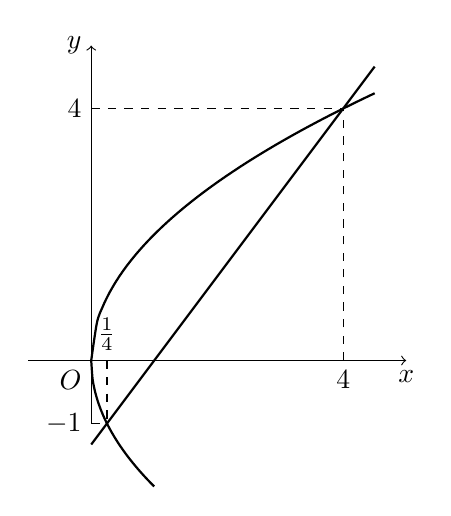
\begin{tikzpicture}[scale=0.8]
            \draw[->] (-1,0) -- (5,0) node[below] {$x$};
            \draw[->] (0,-1) --(0,5) node[left] {$y$};

            \node at (0,0) [below left] {$O$};

            \node at (4,0) [below] {4};
            \draw[dashed] (4,0) -- (4,4);
            \node at (0.25,0) [above] {$\frac{1}{4}$};
            \draw[dashed] (0.25,0) -- (0.25,-1);
            \node at (0,4) [left] {4};
            \draw[dashed] (0,4) -- (4,4);
            \node at (0,-1) [left] {$-1$};
            \draw[dashed] (0,-1) -- (0.25,-1);

            \draw[domain=0:4.5,samples=50,smooth,thick,black]
            plot (\x,{sqrt(4*\x)});
            \draw[domain=0:1,samples=50,smooth,thick,black]
            plot (\x,-{sqrt(4*\x)});
            \draw[domain=0:4.5,samples=50,smooth,thick,black]
            plot (\x,4/3*\x-4/3);

            \end{tikzpicture}
        \end{center}
        
        可发现围成的图形分为两段:$x\in(0,\frac{1}{4})$时上下都是$y^2=4x$\ (事实上上方为$y=2\sqrt{x}$、下方为$-2\sqrt{x}$),$x\in(\frac{1}{4},1)$时上方为$y^2=4x$\ (事实上为$y=2\sqrt{x}$)、下方为$4x-3y=4$\ (即$y=\frac{4}{3}(x-1)$),由此写出积分
        $$\int_0^{1/4}(2\sqrt{x}-(-2\sqrt{x}))\dr x+\int_{1/4}^4\bigg(2\sqrt{x}-\frac{4}{3}(x-1)\bigg)\dr x$$
        利用$\sqrt{x}$的原函数为$\frac{2}{3}x^{3/2}$、$x-1$的原函数为$\frac{1}{2}(x-1)^2$,即可用微积分基本定理算得结果为
        $$\frac{1}{3}+\frac{117}{24}=\frac{125}{24}$$

        \note 事实上``横过来看''此图后对$y$积分将更为简单,不过事实上我们之后才会学到此技巧的本质。
    }

    \item (习题2.10.2)验证$F(x)=\frac{1}{2}x^2-\frac{1}{x}$是$f(x)=x+\frac{1}{x^2}$的一个原函数,并计算积分
    $$\int_2^4\bigg(x+\frac{1}{x^2}\bigg)\dr x$$
    说明以下两式是否相等:
    $$\int_{-1}^1\bigg(x+\frac{1}{x^2}\bigg)\dr x,\quad\bigg(\frac{1}{2}x^2-\frac{1}{x}\bigg)\bigg|^1_{-1}$$

    \sol{
        直接求导即可验证。由于在$[2,4]$区间$f(x)$连续且$F(x)$处处导数为$f(x)$,由微积分基本定理可知积分为
        $$F(4)-F(2)=\frac{25}{4}$$
        下面两式并不等,这是由于$[-1,1]$区间$f(x)$\textbf{不连续},不满足为微积分基本定理使用条件。

        \note 并不只有不连续会导致不满足使用条件,注意\exref{not nl formula}这类情况。
    }

    \item (习题2.10.3(3))视为适当函数的黎曼和极限以计算极限:
    $$\lim_{n\to\infty}\sum_{k=1}^n\frac{1}{n+k}$$
    
    \sol{
        为了配凑出黎曼和,我们需要先\textbf{提出$\frac{1}{n}$}将其写为
        $$\lim_{n\to\infty}\frac{1}{n}\sum_{k=1}^n\frac{1}{1+\frac{k}{n}}$$

        考虑$f(x)=\frac{1}{1+x}$,将区间$(0,1)$进行$n$等分后,记$x_i=\frac{i}{n}$,可发现上式为
        $$\sum_{k=1}^nf(x_i)(x_i-x_{i-1})$$
        由于$f(x)$在0到1的定积分存在,而$n\to\infty$时区间长度趋于0,利用定积分定义可知(由$\frac{1}{1+x}$的一个原函数为$\ln(1+x)$)
        $$\lim_{n\to\infty}\sum_{k=1}^n\frac{1}{n+k}=\int_0^1\frac{1}{1+x}\dr x=\ln 2$$

    }
    \note 配成黎曼和本质上需要配凑为
    $$\frac{1}{n}\sum_{k=1}^nf\bigg(\frac{k}{n}\bigg)$$
    的形式,更多技巧将在下一章介绍。

    \item (习题2.10.4(3))看作分段函数以计算
    $$\int_0^1x\bigg|\frac{1}{2}-x\bigg|\dr x$$

    \sol{
        将被积函数$f(x)$写为分段函数
        $$f(x)=\begin{cases}\frac{1}{2}x-x^2&x\in[0,\frac{1}{2}]\\x^2-\frac{1}{2}x&x\in(\frac{1}{2},1]\end{cases}$$
        由
        $$\int_0^1f(x)\dr x=\int_0^{1/2}f(x)\dr x+\int_{1/2}^1f(x)\dr x$$
        展开后通过幂函数原函数结论,对每段利用微积分基本定理即可算出结果为$\frac{1}{8}$。
    }

    \item (3.1节例8)计算
    $$\int\frac{\dr x}{\sin x}$$

    \sol{
        这里我们采用一个有一定技巧性的方式(事实上之后可学到本质原因):分子分母同乘$\sin x$将其化为
        $$\int\frac{\sin x\dr x}{\sin^2x}$$
        分子实际上是$-\dr\cos x$,而分母也可以化为$1-\cos^2x$,由此代换$t=\cos x$可发现
        $$\int\frac{\dr x}{\sin x}=\int\frac{-\dr t}{1-t^2}$$
        此时已经可以裂项计算
        $$\int\frac{-\dr t}{1-t^2}=\frac{1}{2}\int\bigg(\frac{1}{t-1}-\frac{1}{t+1}\bigg)\dr t=\frac{1}{2}(\ln|t-1|-\ln|t+1|)+C$$
        将$t$代换回$x$可得到
        $$\frac{1}{2}\ln\frac{|\cos x-1|}{|\cos x+1|}+C$$
        
        \note 注意$\frac{1}{x}$的积分\textbf{不要忘记绝对值}。虽然我们并不会严格讨论不定积分的定义范围,但积分完后的定义域应为与原本相同(或至多挖去一些点),本章将部分进行讨论。
    }

    \note \textbf{对某变量的不定积分得到的是该变量的函数},因此换元后需要换回来。这与之后学习的定积分换元方式有本质差别。

    \item (3.1节例14)已知常数$a>0$,计算
    $$\int\frac{\dr x}{\sqrt{x^2-a^2}}$$

    \sol{
        分为三步:
        \begin{itemize}
            \item \textbf{化简}
            
            利用三角函数关系,代入$x=a\frac{1}{\cos t}$\ (即$t=\arccos\frac{a}{x}$,由$x$定义域其可行)可消除根号项得到
            $$\frac{1}{\sqrt{x^2-a^2}}=\frac{1}{a|\tan t|}$$
            从而(在$\arccos$的值域$[0,\pi]$内$\sin t$恒非负)
            $$\int\frac{\dr x}{\sqrt{x^2-a^2}}=\int\frac{-\sin t\dr t}{|\sin t\cos t|}=\int\frac{\dr t}{|\cos t|}$$

            对$x>a$的范围,对应的$t\in(0,\frac{\pi}{2})$,由此上式为$\int\frac{\dr t}{\cos t}$,否则上式为$-\int\frac{\dr t}{\cos t}$。

            \item \textbf{计算积分}
            
            与前一题思路完全相同,代入$s=\sin t$可得
            $$\int\frac{\dr t}{\cos t}=\int\frac{\cos t\dr t}{\cos^2t}=\int\frac{1}{1-s^2}\dr s=-\frac{1}{2}\ln\frac{|s-1|}{|s+1|}+C$$
            将负号合并到$\ln$中最终得到
            $$\int\frac{\dr t}{\cos t}=\frac{1}{2}\ln\frac{|\sin t+1|}{|\sin t-1|}+C$$

            \item \textbf{计算三角}
            
            在进行最终化简前,我们需要计算$\sin\arccos y$。根据定义,它指的是$\cos$一个角为$y$时这个角的$\sin$值,且由$\arccos$值域$[0,\pi]$可知$\sin$值为正,因此有
            $$\sin\arccos y=\sqrt{1-y^2}$$
            从而进一步可知(分子分母同乘$|x|$)
            $$\frac{\sin t+1}{\sin t-1}=\frac{\sin\arccos\frac{a}{x}+1}{\sin\arccos\frac{a}{x}-1}=\frac{\sqrt{x^2-a^2}+|x|}{\sqrt{x^2-a^2}-|x|}$$
            进行分母有理化即可发现
            $$\frac{\sin t+1}{\sin t-1}=\frac{(\sqrt{x^2-a^2}+|x|)^2}{-a^2}$$
            从而
            $$\frac{1}{2}\ln\frac{|\sin t-1|}{|\sin t+1|}+C=\ln|\sqrt{x^2-a^2}+|x||-\ln a+C$$
            常数部分$-\ln a$可合并到常数中,得到(这里$C$为任意常数,但与之前的$C$含义不同,详见本讲义6.2.1的讨论)
            $$\int\frac{\dr t}{\cos t}=\ln|\sqrt{x^2-a^2}+|x||+C$$
        
            \item \textbf{合并}
            
            由上述讨论,分$x>a$与$x<-a$,我们最终得到原不定积分的结果为
            $$\int\frac{\dr x}{\sqrt{x^2-a^2}}=\begin{cases}\ln|\sqrt{x^2-a^2}+x|+C&x>a\\-\ln|\sqrt{x^2-a^2}-x|+C&x<-a\end{cases}$$
            最后,再次使用分子有理化有
            $$-\ln|\sqrt{x^2-a^2}-x|=\ln\frac{1}{|\sqrt{x^2-a^2}-x|}=\ln|\sqrt{x^2-a^2}+x|-2\ln a$$
            从而与之前类似将$C$代换为$-2\ln a+C$即得最终统一为
            $$\int\frac{\dr x}{\sqrt{x^2-a^2}}=\ln|\sqrt{x^2-a^2}+x|+C$$
        \end{itemize}
    }

    \note 遇到$\sqrt{\pm x^2\pm a^2}$类式子应优先使用\textbf{三角换元}化简。

    \note 不定积分一定要\textbf{记忆}一些重要结论(像此题几乎不可能现推出来),具体将在本章介绍。

    \item (习题3.1.4)计算
    $$\int(2x^{3/2}+1)^{2/3}\sqrt{x}\dr x$$

    \sol{
        由于内部都和$\sqrt{x}$有关,我们先设$t=\sqrt{x}$,即$x=t^2$,上述不定积分即改为
        $$\int2(2t^3+1)^{2/3}t^2\dr t$$
        注意这里$t^2\dr t$可以凑出$t^3$,由此进一步设$s=2t^3$\ (直接设$t^3$也可以,这里直接进行了简化)得到
        $$\int\frac{1}{3}(s+1)^{2/3}\dr s$$
        利用幂函数求导公式可直接得上式为
        $$\frac{1}{5}(s+1)^{5/3}+C$$
        代回$x$即得不定积分结果
        $$\frac{1}{5}(2x^{3/2}+1)^{5/3}+C$$
        
        \note 注意设$t=\sqrt{x}$时需要关注\textbf{定义域}是否保证了$x\ge0$。
    }

    \item (习题3.1.8)计算
    $$\int\frac{1}{\sqrt{7-3x^2}}\dr x$$
    
    \sol{
        由于已知$\arcsin x$的导数为$\frac{1}{\sqrt{1-x^2}}$,我们设法向这个方向凑,可发现原式为
        $$\frac{1}{\sqrt7}\int\frac{1}{\sqrt{1-(\sqrt{3/7}x)^2}}\dr x=\frac{1}{\sqrt3}\int\frac{1}{\sqrt{1-(\sqrt{3/7}x)^2}}\dr (\sqrt{3/7}x)=\frac{1}{\sqrt3}\arcsin\bigg(\sqrt{\frac{3}{7}}x\bigg)$$

        \note 利用\textbf{一次函数}(即$ax+b$的形式)进行配凑是不定积分最基本的配凑方式。
    }

    \item (习题3.1.12)计算
    $$\int\frac{\dr x}{\er^x-\er^{-x}}$$

    \sol{
        利用$\dr x=\frac{\dr\er^x}{\er^x}$,如果原式\textbf{可以看成$\er^x$的函数},直接进行换元$t=\er^x$即可得到$x$的函数,对本题来说效果为
        $$\int\frac{\dr x}{\er^x-\er^{-x}}=\int\frac{\dr\er^x}{\er^{2x}-1}=\int\frac{\dr t}{t^2-1}=\frac{1}{2}\ln\frac{|1-t|}{|1+t|}+C$$
        这里最后一步计算在本部分第13题已经进行了。由此可得最终结果为
        $$\frac{1}{2}\ln\frac{|1-\er^x|}{|1+\er^x|}+C$$
    }

    \item (习题3.1.16)计算
    $$\int\frac{x^{14}\dr x}{(x^5+1)}$$

    \sol{
        从形式可观察出希望将$x^5$作为整体,而分子的$x$次数又保证了这件事的可行性。令$t=x^5$可将原式化为
        $$\frac{1}{5}\int\frac{t^2\dr t}{(t+1)^4}$$
        由于分母的$t+1$相对难处理,我们将它看作整体,令$s=t+1$将原式化为
        $$\frac{1}{5}\int\frac{(s-1)^2\dr s}{s^4}$$
        这样就可以直接展开算出积分结果为
        $$\frac{1}{5}\bigg(-\frac{1}{s}+\frac{1}{s^2}-\frac{1}{3s^3}\bigg)$$
        代回$x$即得不定积分结果
        $$\frac{1}{5}\bigg(-\frac{1}{x^5+1}+\frac{1}{(x^5+1)^2}-\frac{1}{3(x^5+1)^3}\bigg)$$
    }

    \item (习题3.1.20)计算
    $$\int\frac{\er^{\arctan x}+x\ln(1+x^2)}{1+x^2}\dr x$$
    
    \sol{
        这题最关键的是将它\textbf{拆分}为两部分
        $$\int\frac{\er^{\arctan x}}{1+x^2}\dr x+\int\frac{x\ln(1+x^2)}{1+x^2}\dr x$$
        分别处理。

        对第一部分,利用$\frac{\dr x}{1+x^2}=\dr\arctan x$可以直接得到其为
        $$\er^{\arctan x}+C$$
        对第二部分,由于除了$x\dr x$外其他部分均为$x^2$,将$1+x^2$看作整体,令$t=1+x^2$换元后得到其为(注意$t>0$,无需绝对值)
        $$\frac{1}{2}\int\frac{\ln t}{t}\dr t=\frac{1}{2}\int\ln t\dr\ln t=\frac{1}{4}\ln^2t+C$$
        两部分合并即得到不定积分结果
        $$\er^{\arctan x}+\frac{1}{4}\ln^2(x^2+1)+C$$
    }

    \item (习题3.1.24)计算
    $$\int\frac{2x-1}{\sqrt{1-x^2}}\dr x$$

    \sol{
        本题同样直接拆分即可:原式为
        $$\int\frac{2x}{\sqrt{1-x^2}}\dr x-\int\frac{1}{\sqrt{1-x^2}}\dr x=\int\frac{\dr x^2}{\sqrt{1-x^2}}-\arcsin x+C$$
        进一步计算,将分母中的$1-x^2$看作整体,令$t=1-x^2$进一步化简得到其为
        $$-\int\frac{\dr t}{\sqrt{t}}-\arcsin x+C=-2\sqrt{t}-\arcsin x+C=-2\sqrt{1-x^2}-\arcsin x+C$$

    }

    \item (习题3.1.28)已知常数$a>0$,计算
    $$\int\frac{x^2}{\sqrt{a^2-x^2}}\dr x$$

    \sol{
        在教材3.1节例12中已经算出
        $$\int\sqrt{a^2-x^2}\dr x=\frac{a^2}{2}\arcsin\frac{x}{a}+\frac{x}{2}\sqrt{a^2-x^2}+C$$
        与本部分第15题完全相同可得
        $$\int\frac{\dr x}{\sqrt{a^2-x^2}}=\arcsin\frac{x}{a}+C$$
        向这两个形式去配凑可发现原式为
        $$\int\frac{a^2-(a^2-x^2)}{\sqrt{a^2-x^2}}\dr x=a^2\int\frac{1}{\sqrt{a^2-x^2}}\dr x-\int\sqrt{a^2-x^2}\dr x$$
        代入即得结果为
        $$\frac{a^2}{2}\arcsin\frac{x}{a}-\frac{x}{2}\sqrt{a^2-x^2}+C$$
    }

    \item (习题3.1.32)计算
    $$\int\frac{\er^{2x}}{\sqrt[3]{1+\er^x}}\dr x$$

    \sol{
        如本部分第16题所说,这类题目可以直接换元$t=\er^x$,由分母形式我们再换元$s=t+1$,即得
        $$\int\frac{\er^{2x}}{\sqrt[3]{1+\er^x}}\dr x=\int\frac{t\dr t}{\sqrt[3]{1+t}}=\int\frac{(s-1)\dr s}{\sqrt[3]{s}}$$
        直接利用幂函数原函数即得到积分为
        $$\frac{3}{5}s^{\frac{5}{3}}-\frac{3}{2}s^{\frac{2}{3}}+C$$
        代回$x$即得不定积分结果
        $$\frac{3}{5}(\er^x+1)^{\frac{5}{3}}-\frac{3}{2}(\er^x+1)^{\frac{2}{3}}+C$$
    }

    \item (3.2节例8)已知常数$a$、$b$大于0,计算
    $$\int\er^{ax}\cos(bx)\dr x$$

    \sol{
        由于
        $$(f(x)\er^{ax})'=(af(x)+f'(x))\er^{ax}$$
        而$\cos(bx)$导数为$-b\sin(bx)$、$\sin(bx)$导数为$b\cos(bx)$,可以想到待定系数求解
        $$\frac{\dr}{\dr x}(c_1\sin(bx)+c_2\cos(bx))\er^{ax}=\cos(bx)\er^{ax}$$
        通过此式对比左右$\cos(bx)\er^{ax}$与$\sin(bx)\er^{ax}$的系数可解出
        $$c_1=\frac{b}{a^2+b^2},\quad c_2=\frac{a}{a^2+b^2}$$
        由此最终结果为
        $$\frac{a\cos(bx)+b\sin(bx)}{a^2+b^2}\er^{ax}+C$$
    }
    
    \note 教材方法的\textbf{严谨性}需要非常复杂的说明,详见本讲义6.2.1。

    \note 另一个可以考虑的计算方法是\textbf{复数},但\textbf{仅能用于得出结果},以此写过程将被扣分,本章将介绍一些相关的技巧。

    \item (习题3.2.3)计算
    $$\int x\sin(2x)\dr x$$
    \sol{
        由于$\sin(2x)\dr x=-\frac{1}{2}\dr\cos(2x)$,分部积分可得原式为
        $$-\frac{1}{2}\int x\dr\cos(2x)=-\frac{1}{2}x\cos(2x)+\frac{1}{2}\int\cos(2x)\dr x=-\frac{1}{2}x\cos(2x)+\frac{1}{4}\sin(2x)$$
    }

    \item (习题3.2.6)计算
    $$\int\er^{2x}\cos(3x)\dr x$$

    \sol{
        直接由本部分第22题结论可知积分结果为
        $$\frac{2\cos(3x)+3\sin(3x)}{13}\er^{2x}$$
    }
    \item (习题3.2.9)计算
    $$\int\sqrt{1+9x^2}\dr x$$

    \sol{
        在教材3.2节例6中已经算出
        $$\int\sqrt{a^2+x^2}\dr x=\frac{a^2}{2}\ln|x+\sqrt{a^2+x^2}|+\frac{x}{2}\sqrt{a^2+x^2}+C$$
        从而有
        $$\int\sqrt{1-9x^2}\dr x=3\int\sqrt{1/3^2-x^2}\dr x=\frac{1}{6}\ln\bigg|x+\sqrt{\frac{1}{9}+x^2}\bigg|+\frac{x}{2}\sqrt{1+9x^2}+C$$

        \note 也可加常数$\frac{1}{6}\ln 3$进一步化简$\ln$中的表达式,不过上式已经足以作为结果。
    }
    
    \item (习题3.2.12)计算
    $$\int\arccos^2x\dr x$$

    \sol{
        当遇到整体不好处理的式子时,可以尝试\textbf{直接分部},也即将积分改写为
        $$x\arccos^2x-\int x\dr\arccos^2x=x\arccos^2x+\int\frac{2x}{\sqrt{1-x^2}}\arccos x\dr x$$
        为了进一步计算,换元$t=1-x^2$可以直接得到
        $$\int\frac{2x\dr x}{\sqrt{1-x^2}}=-\int\frac{\dr t}{\sqrt t}=-2\sqrt{t}=-2\sqrt{1-x^2}$$

        \note 这步的目的是计算出的\textbf{$\arccos x$外的部分的原函数},以进一步进行分部。

        由此有
        $$\begin{aligned}\int\frac{2x}{\sqrt{1-x^2}}\arccos x\dr x&=\int\arccos x\dr(-2\sqrt{1-x^2})\\ &=-2\sqrt{1-x^2}\arccos x+2\int\sqrt{1-x^2}\dr\arccos x\\ &=-2\sqrt{1-x^2}\arccos x-2\int1\dr x=-2\sqrt{1-x^2}\arccos x-2x+C\end{aligned}$$
        从而最终结果为
        $$x\arccos^2x-2\sqrt{1-x^2}\arccos x-2x+C$$
    }

    \item (习题3.2.15)计算
    $$\int\frac{\arcsin x}{x^2}\dr x$$
    
    \sol{
        保留$\arcsin x$合并其他部分由分部积分可得此为
        $$-\int\arcsin x\dr\frac{1}{x}=-\frac{\arcsin x}{x}+\int\frac{\dr x}{x\sqrt{1-x^2}}$$
        下面考虑剩下的积分,由于除了分母的$x$外均为$x$的奇数次方,可以想到分子分母同乘$x$配凑为$\dr x^2$,设$t=x^2$可得
        $$\int\frac{\dr x}{x\sqrt{1-x^2}}=\frac{1}{2}\int\frac{\dr t}{t\sqrt{1-t}}$$
        由于$\sqrt{1-t}$难以处理,设为整体$s=\sqrt{1-t}$,则$t=1-s^2$,计算可得
        $$\frac{1}{2}\int\frac{\dr t}{t\sqrt{1-t}}=-\int\frac{\dr s}{1-s^2}=\frac{1}{2}\ln\frac{|s-1|}{|s+1|}$$
        最终代入可得到不定积分为
        $$-\frac{\arcsin x}{x}+\frac{1}{2}\ln\frac{|\sqrt{1-x^2}-1|}{|\sqrt{1-x^2}+1|}+C$$

        \note 由于$x\ne0$,$|\sqrt{1-x^2}-1|\ne0$,也可以对$\ln$中的部分进行分母有理化化简,得到
        $$\frac{1}{2}\ln\frac{|\sqrt{1-x^2}-1|}{|\sqrt{1-x^2}+1|}=\frac{1}{2}\ln\frac{(\sqrt{1-x^2}-1)^2}{x^2}=\ln\frac{|\sqrt{1-x^2}-1|}{|x|}$$
    }

    \item (习题3.2.18)计算
    $$\int x\ln(x+\sqrt{1+x^2})\dr x$$

    \sol{
        直接计算可发现$\ln(x+\sqrt{1+x^2})$导数为$\frac{1}{\sqrt{1+x^2}}$,从而保留$\ln$部分由分部积分可知原式为
        $$\frac{1}{2}\int\ln(x+\sqrt{1+x^2})\dr x^2=\frac{1}{2}x^2\ln(x+\sqrt{1+x^2})-\frac{1}{2}\int\frac{x^2}{\sqrt{1+x^2}}\dr x$$
        与本部分第20题类似,利用$\frac{x^2}{\sqrt{1+x^2}}=\sqrt{1+x^2}-\frac{1}{\sqrt{1+x^2}}$,由$\ln(x+\sqrt{1+x^2})$导数为$\frac{1}{\sqrt{1+x^2}}$与教材3.2节例6可得
        $$\int\frac{x^2}{\sqrt{1+x^2}}\dr x=\frac{x}{2}\sqrt{1+x^2}-\frac{1}{2}\ln(x+\sqrt{1+x^2})+C$$
        从而最终结果为
        $$\frac{1}{2}x^2\ln(x+\sqrt{1+x^2})-\frac{x}{4}\sqrt{1+x^2}+\frac{1}{4}\ln(x+\sqrt{1+x^2})+C$$
    }
    
    \note \textbf{反三角函数}、\textbf{对数函数}求导后就将成为幂函数的加减乘除与复合,从而都常用分部积分处理。
\end{enumerate}

\subsection{不定积分}
\subsubsection{换元与配凑}
不定积分最基本的方法是\textbf{换元法},分为两种情况(默认里面提及导数的函数都可导):
\begin{itemize}
    \item \textbf{凑微分},即若原不定积分能看成
    $$\int g(f(x))f'(x)\dr x$$
    的形式,我们代入$t=f(x)$可发现上式为
    $$\int g(f(x))\dr f(x)=\int g(t)\dr t$$
    \item \textbf{代入换元},即对任何不定积分
    $$\int g(x)\dr x$$
    我们可以直接代入$x=h(t)$使得其化为
    $$\int g(h(t))\dr h(t)=\int g(h(t))h'(t)\dr t$$
\end{itemize}

当然,为了知道配凑成何种形式就可以算出了,大家\textbf{必须}记熟基本初等函数的导数结果,且\textbf{非常推荐}记忆教材3.2节结尾列出的不定积分公式。

不过,值得注意的额是,上述做法事实上存在诸多严谨性问题:
\begin{itemize}
    \item $\dr f(x)=f'(x)\dr x$是针对\textbf{微分}而言的,而我们从来没有解释过不定积分$\int f(x)\dr x$中的$\dr x$和微分$\dr x$有什么关系。
    \item 以凑微分为例,假设$g(t)$的一个原函数是$G(t)$,有$(G(f(x)))'=G'(f(x))f'(x)=g(f(x))f'(x)$,这样可以从形式上证明换元的正确性,但即使如此,我们在上述讨论中\textbf{几乎完全忽略了定义域问题},这可能导致一些非常麻烦的情况。
\end{itemize}

由于不定积分在本课程要求中只需学会计算技巧,目前我们只强调一件事,即换元$x=h(t)$时应\textbf{保证存在函数$g$使得$g(h(t))=x$}\ (事实上如果有部分端点不满足此式也问题不大)。可以证明,在做到这件事后,不定积分换元计算\textbf{在区间上}能得到正确的结果。

\note 由此建议大家\textbf{优先使用凑微分},因为这几乎不会遇到严谨性问题。

\note 当然,实际做题时也可能会出现一些特殊的情况,由此还是建议大家养成计算完不定积分后\textbf{求导检验结果与结果定义域}的习惯。

最后,仍然注意对$x$不定积分得到的是含$x$的表达式,对$t$不定积分得到的是含$t$的表达式,最后\textbf{须把$t$代换回$x$}。

\

我们来做一些基本的练习:
\begin{framed}
\begin{exercise}
    计算
    $$\int\frac{1}{\er^x-1}\dr x$$
\end{exercise}
\sol{
    由于$\dr\er^x=\er^x\dr x$,我们可以直接将其配凑为
    $$\int\frac{\dr\er^x}{(\er^x-1)\er^x}$$
    由于$\er^x\ne0$,这样做也不会影响定义域。设$t=\er^x$即有上式为
    $$\int\frac{\dr t}{t(t-1)}=\int\frac{\dr t}{t-1}-\int\frac{\dr t}{t}=\ln|t-1|-\ln|t|+C$$
    代入即得原积分为
    $$\ln|\er^x-1|-x+C$$

    \note 所有$\int f(\er^x)\dr x$均可类似处理。
}
\end{framed}

\begin{framed}
\begin{exercise}
    计算
    $$\int\frac{\dr x}{x\sqrt{x^2-1}}$$
\end{exercise}
\sol{
    介绍两种不同的换元思路:
    \begin{itemize}
        \item \textbf{凑微分思路}
        
        由于分母除了$x^2$相关的项只有$x$,想到分子分母同乘$x$,换元$t=x^2$得到原式为
        $$\frac{1}{2}\int\frac{\dr t}{t\sqrt{t-1}}$$
        由于$\sqrt{t-1}$难以处理,我们考虑将其看作整体,而恰好有
        $$\frac{\dr t}{\sqrt{t-1}}=2\dr\sqrt{t-1}$$
        从而再令$s=\sqrt{t-1}$,有$t=s^2+1$,将其进一步写为
        $$\int\frac{\dr s}{s^2+1}=\arctan s+C$$
        代入即得原积分为
        $$\arctan\sqrt{x^2-1}+C$$

        \note 这里有两个基本技巧,一个是熟悉\textbf{基本初等函数}的导数,另一个是由\textbf{复合函数导数}有$\dr f(ax+b)=af'(ax+b)\dr x$,因此若看到$f'$复合\textbf{一次函数}的形式,也可以直接配为$f(ax+b)$的微分。这里对$\sqrt{t-1}$就是如此处理的。

        \item \textbf{代入换元思路}
    
        由于分母出现了$\sqrt{x^2-1}$,我们尝试使用三角换元,设$x=\frac{1}{\cos t}$\ (此时利用定义域可发现$t=\arccos\frac{1}{x}$,符合换元要求),代入并计算可发现积分化为
        $$\int \frac{\sin t\dr t}{\cos t\sqrt{\frac{\sin^2t}{\cos^2t}}}\dr t=\int\frac{\tan t}{|\tan t|}\dr t$$
        当$x>1$时,$t\in(0,\frac{\pi}{2})$,对应积分即为$\int1\dr t=t+C$,结果为
        $$\arccos\frac{1}{x}+C$$
        当$x<-1$,$t\in(\frac{\pi}{2},\pi)$,对应积分即为$\int(-1)\dr t=-t+C$,结果为
        $$-\arccos\frac{1}{x}+C$$

        \note 由此可见,为了过程的严谨性,\textbf{当$x$定义域分为多段时最好分别讨论}。
    \end{itemize}

    \note 注意到两种做法得出的结果形式上并不同,涉及反三角函数与$\ln$时尤其容易出现这类情况,仍然注意\textbf{求导验算}。

    \note 本题事实上还有换元$x=\frac{1}{t}$等做法,大家可以自己尝试,积分计算的方法往往是灵活的。
}
\end{framed}

\

涉及\textbf{三角}时,情况往往会更加复杂:
\begin{framed}
\begin{exercise}
    计算
    $$\int\sqrt{1+\sin x}\dr x$$
\end{exercise}
\sol{
    介绍两种方法:
    \begin{itemize}
        \item \textbf{观察结构}
        
        如果大家对二倍角公式足够敏感,可以发现
        $$1+\sin x=1+2\sin\frac{x}{2}\cos\frac{x}{2}=\bigg(\sin\frac{x}{2}+\cos\frac{x}{2}\bigg)^2$$
        由此原积分实质上是
        $$\int\bigg|\sin\frac{x}{2}+\cos\frac{x}{2}\bigg|\dr x$$
        不过,我们并未学过任何绝对值相关的积分结论。至此有两种不同思路:
        \begin{enumerate}
            \item 回到\textbf{微积分基本定理}:由于此函数在$\rb$上连续,它的所有原函数可以写为
            $$\int_0^x\bigg|\sin\frac{s}{2}+\cos\frac{s}{2}\bigg|\dr s+C$$
            只要分段讨论计算此积分即可,由于我们这里介绍的是不定积分计算技巧,不详细介绍此思路。

            \item 还是利用\textbf{原函数}的思路计算,设它的一个原函数为$F(x)$。首先,为了确定绝对值何时取正,我们将其进行一些配凑(这理应是高中阶段的三角函数技巧)
            $$\bigg|\sin\frac{x}{2}+\cos\frac{x}{2}\bigg|=\sqrt{2}\bigg|\frac{\sqrt2}{2}\sin\frac{x}{2}+\frac{\sqrt2}{2}\cos\frac{x}{2}\bigg|=\sqrt{2}\bigg|\sin\bigg(\frac{x}{2}+\frac{\pi}{4}\bigg)\bigg|$$
            由此,利用三角函数性质,此函数可以进一步写为
            $$\begin{cases}\sqrt{2}\sin\big(\frac{x}{2}+\frac{\pi}{4}\big)&x\in\big[-\frac{\pi}{2}+4k\pi,\frac{3\pi}{2}+4k\pi\big)\\-\sqrt{2}\sin\big(\frac{x}{2}+\frac{\pi}{4}\big)&x\in\big[\frac{3\pi}{2}+4k\pi,\frac{7\pi}{2}+4k\pi\big)\end{cases},\quad\forall k\in\mathbb{Z}$$
            
            直接利用复合一次函数的结论可知
            $$\int\sqrt2\sin\bigg(\frac{x}{2}+\frac{\pi}{4}\bigg)=-2\sqrt2\cos\bigg(\frac{x}{2}+\frac{\pi}{4}\bigg)+C$$
            由此考虑每个开区间可知,必然存在常数$C_k$、$D_k$\ ($k\in\mathbb{Z}$)使得
            $$F(x)=\begin{cases}-2\sqrt{2}\cos\big(\frac{x}{2}+\frac{\pi}{4}\big)+C_k&x\in\big(-\frac{\pi}{2}+4k\pi,\frac{3\pi}{2}+4k\pi\big)\\2\sqrt{2}\cos\big(\frac{x}{2}+\frac{\pi}{4}\big)+D_k&x\in\big(\frac{3\pi}{2}+4k\pi,\frac{7\pi}{2}+4k\pi\big)\end{cases},\quad\forall k\in\mathbb{Z}$$

            由于$F$在$\rb$上可导,必然连续,考虑所有
            $$\frac{3\pi}{2}+4k\pi$$
            处的左右极限可以发现
            $$-2\sqrt{2}\cos\bigg(\frac{3\pi}{4}+\frac{\pi}{4}\bigg)+C_k=2\sqrt{2}\cos\bigg(\frac{3\pi}{4}+\frac{\pi}{4}\bigg)+D_k$$
            从而$D_k=C_k+4\sqrt2$,而考虑所有$\frac{7\pi}{2}+4k\pi$处可发现
            $$-2\sqrt{2}\cos\bigg(\frac{7\pi}{4}+\frac{\pi}{4}\bigg)+C_{k+1}=2\sqrt{2}\cos\bigg(\frac{7\pi}{4}+\frac{\pi}{4}\bigg)+D_k$$
            从而$C_{k+1}=D_k+4\sqrt2$。

            由于$F(x)$加实数仍为原函数,可不妨设$C_0=0$,从以上两式可递推出$C_k=8\sqrt2k$、$D_k=8\sqrt2k+4\sqrt2$,再结合$F(x)$连续性最终得到表达式
            $$F(x)=\begin{cases}-2\sqrt{2}\cos\big(\frac{x}{2}+\frac{\pi}{4}\big)+8\sqrt2k&x\in\big[-\frac{\pi}{2}+4k\pi,\frac{3\pi}{2}+4k\pi\big)\\2\sqrt{2}\cos\big(\frac{x}{2}+\frac{\pi}{4}\big)+8\sqrt2k+4\sqrt2&x\in\big[\frac{3\pi}{2}+4k\pi,\frac{7\pi}{2}+4k\pi\big)\end{cases},\quad\forall k\in\mathbb{Z}$$
            可以由定义验证在所有区间分界点处$F$的导数的确为0,从而$F$是其在$\rb$上的一个原函数,因此
            $$\int\sqrt{1+\sin x}\dr x=F(x)+C$$
        \end{enumerate}

        \item \textbf{直接操作}
        
        本题的一个容易想到的方法是,利用\textbf{将不会处理的部分看作整体}的思路,设$t=1+\sin x$。为了实现凑微分,我们必须凑出一个$\cos x$才能如此换元,由此我们将原式写为
        $$\int\frac{\sqrt{1+\sin x}}{\cos x}\cos x\dr x$$

        然而,$\cos x$与$\sin x$的关系\textbf{并不固定},必须确定区间才能进行换元。例如,对$x\in(-\frac{\pi}{2},\frac{\pi}{2})$,有$\cos x=\sqrt{1-\sin^2x}$,从而换元后可得
        $$\int\sqrt{t}\frac{\dr t}{\sqrt{1-(t-1)^2}}=\int\frac{\dr}{\sqrt{2-t}}=-2\sqrt{2-t}+C$$
        再代入可发现$\sqrt{1+\sin x}$在$(-\frac{\pi}{2},\frac{\pi}{2})$上的一个原函数为
        $$-2\sqrt{1-\sin x}$$
        类似可以得到$\sqrt{1+\sin x}$在$\sin x$的每个\textbf{单调区间}的原函数。不过,为了得到$\rb$上的原函数,仍然需要类似上一种方法的计算。
    \end{itemize}

    \note 一定注意\textbf{非初等函数的原函数可能涉及复杂的讨论},这里出现的绝对值就是例子。
    
    \note 本题也体现了\textbf{检验定义域}的重要性,如果只给出绝对值中大于0与小于0的不同原函数而不进行组合,我们的原函数定义域将无法是$\rb$,实际上并不符合$\rb$上原函数的定义。
}
\end{framed}

\begin{framed}
\begin{exercise}\label{get sin cos deri}
    计算
    $$\int\frac{\cos x}{2\cos x+5\sin x}\dr x$$
\end{exercise}
\sol{
    介绍两种方法:
    \begin{itemize}
        \item \textbf{直接换元}
        
        对这类有$\sin$与$\cos$的式子,一个\textbf{经验}是尝试设$t=\sin x$或$\cos x$或$\tan x$。

        由于此式中$\sin$与$\cos$\textbf{齐次},分子分母同除以$\cos x$得到其为
        $$\int\frac{1}{2+5\tan x}\dr x$$
        令$t=\tan x$,可得原式化为
        $$\int\frac{1}{(2+5t)(1+t^2)}\dr t$$
        此时可利用之后介绍的\textbf{有理函数}积分方法得到积分结果。这里写出一个简单的过程:待定系数可得
        $$\int\frac{1}{(2+5t)(1+t^2)}\dr t=\int\frac{1}{29}\bigg(\frac{25}{2+5t}+\frac{2-5t}{1+t^2}\bigg)\dr t$$
        从而利用
        $$\int\frac{1}{2+5t}\dr t=\frac{1}{5}\ln|2+5t|$$
        $$\int\frac{1}{1+t^2}\dr t=\arctan t$$
        $$\int\frac{t}{1+t^2}\dr t=\frac{1}{2}\int\frac{\dr t^2}{1+t^2}=\frac{1}{2}\ln(1+t^2)$$
        并代入$t=\tan x$可得到形式上的结果
        $$\frac{1}{29}\bigg(5\ln|2+5\tan x|+2\arctan\tan x-\frac{5}{2}\ln(1+\tan^2x)\bigg)+C$$

        我们自然会产生疑问,令$t=\tan x$是否会导致定义域问题?答案是否定的,因为这样的换元是分子分母同乘$1+\tan^2x=\frac{1}{\cos ^2x}$后进行的,换元前已经写成了
        $$\int\frac{\dr\tan x}{(2+5\tan x)(1+\tan^2x)}$$
        由于\textbf{所有部分都是$\tan x$的函数},换元不会出现问题。

        但是,此处的问题出在更前:由于$\cos x$可能为0,分子分母同除以$\cos x$将导致\textbf{原本连续的点从原函数定义域中被剥离了}。为了解决此问题,我们可以将结果写为
        $$\frac{5}{29}\ln\frac{|2+5\tan x|}{\sqrt{1+\tan^2x}}+\frac{2}{29}\arctan\tan x+C$$
        并将左侧分子分母同乘$|\cos x|$、右侧$\arctan\tan x$改写为$x$\ (注意这实际上未必成立,$x$在不同区间时$\arctan\tan x$结果不同),得到一个\textbf{形式上消去了$\tan x$的结果}
        $$\frac{5}{29}\ln|2\cos x+5\sin x|+\frac{2}{29}x+C$$
        可以发现此结果的定义域与$\frac{\cos x}{2\cos x+5\sin x}$相同,且求导的确为$\frac{\cos x}{2\cos x+5\sin x}$,从而这就是不定积分的结果。

        \note 这里的形式上消去如果想要严格书写,需要利用原函数的连续性在每个$\cos x=0$的点进行讨论,将非常复杂。当自己做题遇到这种情况时同样建议\textbf{先形式上化简再检验}。


        \item \textbf{配凑}
        
        本题事实上可以通过巧妙地配凑解决:可以发现
        $$\int\frac{2\cos x+5\sin x}{2\cos x+5\sin x}\dr x=x+C$$
        $$\int\frac{5\cos x-2\sin x}{2\cos x+5\sin x}\dr x=\int\frac{1}{2\cos x+5\sin x}\dr(2\cos x+5\sin x)=\ln|2\cos x+5\sin x|+C$$
        由此待定系数即可得到
        $$\int\frac{\cos x}{2\cos x+5\sin x}\dr x=\frac{2}{29}\int\frac{2\cos x+5\sin x}{2\cos x+5\sin x}\dr x+\frac{5}{29}\int\frac{5\cos x-2\sin x}{2\cos x+5\sin x}\dr x$$
        从而直接得结果
        $$\int\frac{\cos x}{2\cos x+5\sin x}\dr x=\frac{2}{29}x+\frac{5}{29}\ln|2\cos x+5\sin x|+C$$
    \end{itemize}

    \note 由此可见,虽然不定积分往往有多种方法可以算出,但不同方法往往难度差别巨大。但是,在时间有限时,\textbf{与其追求巧妙方法不如用熟悉的笨方法算出结果}——因为思考巧妙方法本身就会花费大量时间。
}
\end{framed}

此外,对于三角函数相关的问题,还常用一个重要的公式,即\textbf{等差数列的正弦求和公式}:对任何实数$k$、$b$,有
$$\sum_{t=0}^n\sin(kt+b)=\frac{\sin\frac{(n+1)k}{2}\sin(\frac{nk}{2}+b)}{\sin\frac{k}{2}}$$
其证明为,左侧乘$\sin\frac{k}{2}$可得
$$\sum_{t=0}^n\sin(kt+b)\sin\frac{k}{2}=\frac{1}{2}\sum_{t=0}^n\bigg(\cos\bigg(kt-\frac{k}{2}+b\bigg)-\cos\bigg(kt+\frac{k}{2}+b\bigg)\bigg)$$
裂项相消即得到
$$\sum_{t=0}^n\sin(kt+b)\sin\frac{k}{2}=\frac{1}{2}\cos\bigg(-\frac{k}{2}+b\bigg)-\frac{1}{2}\cos\bigg(\frac{2n+1}{2}k+b\bigg)$$
再重新利用和差化积公式展开得结论。

\note 只要将上方的$b$改为$\frac{\pi}{2}+b$即可得到$\cos$求和的结果。

利用此公式可以方便地计算一些问题:
\begin{framed}
\begin{exercise}\label{sin nx div sin x}
    对正整数$n\ge2$计算
    $$\int\frac{\sin(nx)}{\sin x}\dr x$$
\end{exercise}
\sol{
    介绍三种方法:
    \begin{itemize}
        \item \textbf{直接方法}
        
        利用等差数列的正弦求和公式
        $$\sum_{t=0}^m\sin(kt+b)=\frac{\sin\frac{(m+1)k}{2}\sin(\frac{mk}{2}+b)}{\sin\frac{k}{2}}$$
        取$k=2x$、$m=n-1$、$b=-(n-1)x+\frac{\pi}{2}$,即得
        $$\frac{\sin(nx)}{\sin x}=\sum_{t=0}^{n-1}\sin\bigg(2xt-(n-1)x+\frac{\pi}{2}\bigg)=\sum_{t=0}^{n-1}\cos((2t-(n-1))x)$$
        
        \note 注意可能$2t=n-1$的项,因此不能直接认为每项积分是$\frac{1}{2t-(n-1)}\sin((2t-(n-1))x)$。

        可以发现此求和实际上是
        $$\cos(-(n-1)x)+\cos(-(n-3)x)+\dots+\cos((n-3)x)+\cos((n-1)x)$$
        利用$\cos(-x)=\cos x$,分奇偶讨论。对正整数$k$,当$n=2k+1$时上式为
        $$1+2\cos(2x)+\dots+2\cos(2kx)$$
        从而原函数为
        $$x+\sin(2x)+\dots+\frac{1}{k}\sin(2kx)+C$$
        当$n=2k$时上式为
        $$2\cos x+\dots+2\cos((2k-1)x)$$
        从而原函数为
        $$2\sin x+\dots+\frac{2}{2k-1}\sin((2k-1)x)+C$$        
        
        \item \textbf{递推方法}
        
        如果无法直接想起等差数列的正弦求和公式,利用归纳的思路,我们试着将
        $$\int\frac{\sin(nx)}{\sin x}\dr x$$
        与更小的$n$建立联系。

        一个直接的想法是拆分,将$\sin(nx)$看作$\sin((n-1)x)\cos x+\cos((n-1)x)\sin x$,这样就有原式为
        $$\int\frac{\sin((n-1)x)\cos x}{\sin x}\dr x+\int\cos(n-1)x\dr x=\int\frac{\sin((n-1)x)\cos x}{\sin x}\dr x+\frac{\sin((n-1)x)}{n-1}+C$$
        利用不定积分作为表达式集合的定义,我们可以将右侧的$+C$删去,将结果写为
        $$\int\frac{\sin((n-1)x)\cos x}{\sin x}\dr x+\frac{\sin((n-1)x)}{n-1}$$
        不过,左侧仍然不是可以计算的形式,我们尝试再分裂一次,这样即将原式写为了
        $$\int\frac{\sin((n-2)x)\cos^2x}{\sin x}\dr x+\int(\cos(n-2)x)\cos x\dr x+\frac{\sin((n-1)x)}{n-1}$$
        可以发现,由于左边出现了$\cos^2x$,我们将其拆为$1-\sin^2x$就能得到$n-2$的情况,也即原积分最终写为了
        $$\int\frac{\sin((n-2)x)}{\sin x}\dr x-\int\sin((n-2)x)\sin x\dr x+\int(\cos(n-2)x)\cos x\dr x+\frac{\sin((n-1)x)}{n-1}$$
        可以发现,二三两项不定积分可以合并为$\cos((n-1)x)$的不定积分,从而即最终得到等式
        $$\int\frac{\sin(nx)}{\sin x}\dr x=\int\frac{\sin((n-2)x)}{\sin x}\dr x+2\frac{\sin((n-1)x)}{n-1}$$
        由此可以递推到$n=0$\ (积分为$C$)或$n=1$\ (积分为$x+C$)的情况,从而得到与第一种方法相同的结果。

        \note 对三角函数相关的问题,常见需要\textbf{两次}拆分/化简的情况,本质上是由于$\sin$或$\cos$求两次导才会出现自身。
        
        \item \textbf{复数方法}

        利用\textbf{欧拉公式}
        $$\er^{\ir\theta}=\cos\theta+\ir\sin\theta$$
        有
        $$\sin\theta=\frac{\er^{\ir\theta}-\er^{-\ir\theta}}{2\ir}$$
        从而原积分可以形式上写为
        $$\int\frac{\er^{n\ir x}-\er^{-n\ir x}}{\er^{\ir x}-\er^{-\ir x}}\dr x$$
        注意$\er^{n\ir x}=(\er^{\ir x})^n$、$\er^{-n\ir x}=(\er^{-\ir x})^n$,由此从$a^n-b^n$的因式分解可知上式进一步改写为
        $$\int\sum_{r=0}^{n-1}(\er^{\ir x})^r(\er^{-\ir x})^{n-1-r}\dr x=\int\sum_{r=0}^{n-1}\er^{(2r-(n-1))\ir x}\dr x$$
        由于$\frac{\sin(nx)}{\sin x}$为实数,上式的虚部必然可以抵消,从而再用欧拉公式展开后提取实部得到原不定积分化为
        $$\int\sum_{r=0}^{n-1}\cos((2r-(n-1))x)\dr x$$
        此后与第一种方法完全相同。

        \note 注意此方法是严格的,因为我们\textbf{仅用复数方法证明了三角恒等式},\textbf{并未真的进行复函数的求导或积分}。
    \end{itemize}
}
\end{framed}

一定要注意三角换元过程的严谨性:若换元$t=g(x)$前我们已经将它配凑为了$f(g(x))\dr g(x)$的形式,直接换元是不会产生严谨性问题的,否则必须进行更复杂的讨论。

\

最后,我们来求解一个微分方程:
\begin{framed}
\begin{exercise}[\extra]
    已知$r^3-4r^2+5r-2=(r-1)^2(r-2)$,求所有函数$f(x)$使得其在$\rb$上满足
    $$f'''(x)-4f''(x)+5f'(x)-2f(x)=0$$
\end{exercise}
\sol{
    \begin{itemize}
        \item \textbf{基本分析}
        
        这里最重要的步骤是一个\textbf{线性代数}的观察:
        $$f'''(x)-4f''(x)+5f'(x)-2f(x)=\bigg(\frac{\dr}{\dr x}-1\bigg)^2\bigg(\frac{\dr}{\dr x}-2\bigg)f(x)$$
        这里对任何函数$g(x)$,我们定义
        $$\bigg(\frac{\dr}{\dr x}+c\bigg)g(x)=\frac{\dr}{\dr x}g(x)+cg(x)$$
        且左侧的``乘法''代表复合,平方代表与自己复合。

        由此,我们可以将
        $$\bigg(\frac{\dr}{\dr x}-1\bigg)^2\bigg(\frac{\dr}{\dr x}-2\bigg)f(x)$$
        解释为:$f(x)$对$x$求导后减两倍自身得到$f_1(x)$,$f_1(x)$对$x$求导后减自身得到$f_2(x)$,$f_2(x)$对$x$求导后减自身得到结果。大家可以验算其的确与$f'''(x)-4f''(x)+5f'(x)-2f(x)$相等。

        \note 至于为何求导可以与多项式一样进行因式分解,本质上是由于求导运算可以一定程度看成\textbf{线性变换},从而它具有多项式运算相似的交换律、结合律、分配律。后续的线性代数课程中将学到。

        
        \item \textbf{回溯计算}
        
        我们沿续上方定义$f_1(x)=f'(x)-2f(x)$、$f_2(x)=f_1'(x)-f_1(x)$,可发现方程化为
        $$f_2'(x)-f_2(x)=0$$
        接下来我们要用最重要的配凑,对于$g'(x)+ag(x)$一类的式子,我们可以\textbf{乘$\er^a$将整体配为导数}。

        方程两侧乘$\er^{-x}$得到
        $$\er^{-x}f_2'(x)-\er^{-x}f_2(x)=0$$
        可以发现左侧即为$(\er^{-x}f_2(x))'$,从而可知存在$C_2\in\rb$使得
        $$\er^{-x}f_2(x)=C_2$$
        也即
        $$f_2(x)=C_2\er^x$$
        进一步计算,由于$f_2(x)=f_1'(x)-f_1(x)$可得
        $$f_1'(x)-f_1(x)=C_2\er^x$$
        同样两侧乘$\er^{-x}$得到
        $$(\er^{-x}f_1(x))'=C_2$$
        从而可知存在$C_1\in\rb$使得
        $$\er^{-x}f_1(x)=C_2x+C_1$$
        也即
        $$f_1(x)=(C_2x+C_1)\er^x$$
        最后,由于$f_1(x)=f'(x)-2f(x)$可得
        $$f'(x)-2f(x)=(C_2x+C_1)\er^x$$
        两侧乘$\er^{-2x}$得到
        $$(\er^{-2x}f(x))'=(C_2x+C_1)\er^{-x}$$
        
        \item \textbf{最终不定积分}
        
        我们现在来计算
        $$\int (C_2x+C_1)\er^{-x}\dr x$$
        这里的关键观察是,利用$(g(x)\er^{-x})=(g'(x)-g(x))\er^{-x}$,取$g(x)=ax+b$,$a$、$b$为实数,有
        $$((ax+b)\er^{-x})'=(a-ax-b)\er^{-x}$$
        从而令$a-b=C_1$、$-a=C_2$,我们就得到了不定积分结果为
        $$\int (C_2x+C_1)\er^{-x}\dr x=(-C_2x+C_2-C_1)\er^{-x}+C$$

        \note 除了待定系数,这个不定积分也可通过分部积分计算。

        因此存在$C_3\in\rb$使得
        $$\er^{-2x}f(x)=(-C_2x-C_2-C_1)\er^{-x}+C_3$$
        也即
        $$f(x)=(-C_2x-C_2-C_1)\er^x+C_3\er^{2x}$$
        将$-C_2$看作新的常数$D_2$,$-C_2-C_1$看作新的常数$D_1$,即得微分方程的全部解为
        $$f(x)=(D_1+D_2x)\er^x+C_3\er^{2x},\quad D_1,D_2,C_3\in\rb$$

        \note 最后一步事实上需要说明$D_1,D_2$与$C_1,C_2$只要确定一组,另一组也唯一确定。这可以直接求解得到。
    \end{itemize}

    \note 利用这种方法可以计算出$f^{(n)}(x)+a_{n-1}f^{(n-1)}(x)+\dots+a_1f'(x)+f(x)=0$的全部解,这里$a_i$均为实数。
}
\end{framed}

\subsubsection{分部积分}
无论是不定积分还是定积分,\textbf{分部积分}的公式都是非常重要的,它对不定积分写为
$$\int f(x)g'(x)\dr x=f(x)g(x)-\int g(x)f'(x)\dr x$$
利用乘积求导公式,此公式在$f$、$g$均可导且两侧的不定积分至少有一侧存在时是可直接证明的。

\note 分部积分的重要性暗示了乘积求导公式是求导非常\textbf{本质}的性质。即使数学学习更深入后导数可以进行各种各样的推广,我们也仍然至少希望乘积求导公式是成立的。

\

有了分部积分后,相关的计算可以更加灵活:
\begin{framed}
\begin{exercise}
    计算
    $$\int\frac{\er^{\arctan x}}{(1+x^2)^{3/2}}\dr x$$
\end{exercise}
\sol{
    由于$\er^{\arctan x}$难以处理,我们将$\arctan x$看作整体,设$t=\arctan x$,则$x=\tan t$,计算可得原式化为
    $$\int\frac{\er^t}{|\cos t|^{-3}}\frac{\dr t}{\cos^2t}=\int\er^t|\cos t|\dr t$$

    \note 注意此处换元是可以无条件进行的,这是由于$\arctan x$是$\rb$上的严格单调连续函数,对任何$t\in(-\frac{\pi}{2},\frac{\pi}{2})$都可以确定唯一的$x$,符合换元法条件。

    由于换元后$t\in(-\frac{\pi}{2},\frac{\pi}{2})$,$\cos t\ge0$,从而上式改写为
    $$\int\er^t\cos t\dr t$$
    由本讲义7.1第22题可直接得到结果,这里我们介绍一个\textbf{两次分部积分}的证法。

    由于$\er^t\dr t=\dr\er^t$,它常常被用来分部积分,也即
    $$\int\er^t\cos t\dr t=\int\cos t\dr\er^t=\er^t\cos t+\int\er^t\sin t\dr t$$
    虽然这样尚没有做完,但我们可以对右侧的不定积分再次分部积分得到
    $$\int\er^t\sin t\dr t=\int\sin t\dr\er^t=\er^t\sin t-\int\er^t\cos t\dr t$$
    由此可发现
    $$\int\er^t\cos t\dr t=\er^t(\cos t+\sin t)-\int\er^t\cos t\dr t$$
    由\exref{inte equa}即解得
    $$\int\er^t\cos t\dr t=\frac{1}{2}\er^t(\cos t+\sin t)+C$$
    从而原积分即为
    $$\frac{1}{2}\er^{\arctan x}(\cos(\arctan x)+\sin(\arctan x))+C$$
}
\end{framed}

\begin{framed}
\begin{exercise}
    计算
    $$\int\frac{x\tan x}{\cos^2x}\dr x$$
\end{exercise}
\sol{
    若删去$x$,本题将是十分好处理的:
    $$\int\frac{\tan x}{\cos^2x}\dr x=\int\frac{\sin x}{\cos^3x}\dr x=-\int\frac{\dr\cos x}{\cos^3x}=\frac{1}{2\cos^2x}$$
    由此,我们尝试将\textbf{可以积分的部分整体放入分部积分},也即利用上式进行计算
    $$\int\frac{x\tan x}{\cos^2x}\dr x=\int x\dr\frac{1}{2\cos^2x}=\frac{x}{2\cos^2x}-\int\frac{\dr x}{2\cos^2x}$$
    这样就可以直接得到结果为
    $$\frac{x}{2\cos^2x}-\frac{1}{2}\tan x+C$$
}
\end{framed}

\begin{framed}
\begin{exercise}
    计算
    $$\int\ln^2(x+\sqrt{x^2+1})\dr x$$
\end{exercise}
\sol{
    这里出现了最外层的无法处理的$\ln$,我们尝试将其\textbf{整体分部},计算得到
    $$\int\ln^2(x+\sqrt{x^2+1})\dr x=x\ln^2(x+\sqrt{x^2+1})-\int\ln(x+\sqrt{x^2+1})\frac{2x}{\sqrt{x^2+1}}\dr x$$
    但是,这里出现的$\ln$仍然无法处理,由此我们还是先计算
    $$\int\frac{x\dr x}{\sqrt{x^2+1}}=\frac{1}{2}\int\frac{\dr(x^2+1)}{\sqrt{x^2+1}}=\sqrt{x^2+1}$$
    这样就可以分部积分得到
    $$\int\ln(x+\sqrt{x^2+1})\frac{x}{\sqrt{x^2+1}}\dr x=\int\ln(x+\sqrt{x^2+1})\dr\sqrt{x^2+1}=\sqrt{x^2+1}\ln(x+\sqrt{x^2+1})-\int1\dr x$$
    也即
    $$\int\ln(x+\sqrt{x^2+1})\frac{2x}{\sqrt{x^2+1}}\dr x=2\sqrt{x^2+1}\ln(x+\sqrt{x^2+1})-2x+C$$
    最终合并即得到原积分为
    $$x\ln^2(x+\sqrt{x^2+1})-2\sqrt{x^2+1}\ln(x+\sqrt{x^2+1})+2x+C$$
}
\end{framed}

\

当然,分部积分也可以用于构造\textbf{递推公式}:
\begin{framed}
\begin{exercise}\label{sin pow x n}
    求出不定积分
    $$\int\sin^nx\dr x$$
    关于正整数$n$的递推公式。
\end{exercise}
\sol{
    \note 本题的想法相对反直觉,建议理解为某种\textbf{尝试的结果}。

    我们尝试分出一个$\sin x$进行分部积分,计算导数得到原式为
    $$-\int\sin^{n-1}x\dr\cos x=-\sin^{n-1}x\cos x+(n-1)\int\cos^2x\sin^{n-2}x\dr x$$
    此时右侧已经出现了$\cos^2x$,将它重新写为$1-\sin^2x$即得
    $$-\int\sin^{n-1}x\dr\cos x=-\sin^{n-1}x\cos x+(n-1)\int\sin^{n-2}x\dr x-(n-1)\int\sin^nx\dr x$$
    由于上式即
    $$\int\sin^nx\dr x=-\sin^{n-1}x\cos x+(n-1)\int\sin^{n-2}x\dr x-(n-1)\int\sin^nx\dr x$$
    移项合并(这可以利用不定积分的表达式集合定义严谨证明)并同乘$\frac{1}{n}$得到
    $$\int\sin^nx\dr x=-\frac{1}{n}\sin^{n-1}x\cos x+\frac{n-1}{n}\int\sin^{n-2}x\dr x$$
    这就是所求的递推公式。

    \note 注意根据我们的证明过程,事实上
    $$n\int\sin^nx\dr x=-\sin^{n-1}x\cos x+(n-1)\int\sin^{n-2}x\dr x$$
    对任何实数$n$成立,但当$n=0$时左侧需要有$+C$。
}
\end{framed}

\subsubsection{有理函数相关}
\textbf{有理函数}是指满足
$$f(x)=\frac{p(x)}{q(x)}$$
其中$p(x)$为多项式、$q(x)$为非零多项式的函数。

教材3.2节给出了对于一般的有理函数进行不定积分的算法与将三角函数化为有理函数积分的\textbf{万能代换法}、将\textbf{根式}化为有理函数的算法。虽然对具体的问题\textbf{往往存在更好的处理方法},但正如之前所说,这样的``笨办法''是最直接且一定能得到结果的,因此\textbf{必须掌握}。

\note 事实上有理函数的分解不仅可以用来计算积分,在计算\textbf{高阶导数}等场合也有很大的作用。

接下来的例子我们都将介绍更好的方法与基本的配凑方法:
\begin{framed}
\begin{exercise}
    计算
    $$\int\frac{1}{1+x^3}\dr x$$
\end{exercise}
\sol{
    \begin{itemize}
        \item \textbf{有理函数基本做法}
        
        直接因式分解$1+x^3=(1+x)(1-x+x^2)$,从而待定系数可得
        $$\frac{1}{1+x^2}=\frac{1}{3}\bigg(\frac{1}{1+x}-\frac{x-2}{1-x+x^2}\bigg)$$
        再利用
        $$\frac{x-2}{1-x+x^2}=\frac{x-2}{(x-1/2)^2+3/4}=\frac{1}{2}\frac{2(x-\frac{1}{2})}{(x-\frac{1}{2})^2+\frac{3}{4}}-\frac{3}{2}\frac{1}{(x-\frac{1}{2})^2+\frac{3}{4}}$$
        进一步配凑,将两项都配凑为可以计算的形式有(第二项也可以直接通过记忆$\frac{1}{a^2+x^2}$的积分结果得到)
        $$\int\frac{x-2}{1-x+x^2}\dr x=\frac{1}{2}\int\frac{\dr(x-\frac{1}{2})^2}{(x-\frac{1}{2})^2+\frac{3}{4}}-\sqrt3\int\frac{\dr(\frac{2}{\sqrt3}x)}{(\frac{2}{\sqrt3}x-\frac{1}{\sqrt3})^2+1}$$
        从而得上述积分结果为
        $$\frac{1}{2}\ln\bigg(\bigg(x-\frac{1}{2}\bigg)^2+\frac{3}{4}\bigg)-\sqrt3\arctan\bigg(\frac{2}{\sqrt3}x-\frac{1}{\sqrt3}\bigg)+C$$
        化简后与第一项结合也即
        $$\frac{1}{3}\bigg(\ln|1+x|-\frac{1}{2}\ln(1-x+x^2)+\sqrt3\arctan\frac{2x-1}{\sqrt3}\bigg)+C$$

        \item \textbf{配凑做法}
        
        利用\exref{get sin cos deri}类似的思路,由$(1+x^3)'=3x^2$有
        $$\int\frac{3x^2}{1+x^3}\dr x=\ln|1+x^3|+C$$
        为了配凑出其他容易计算的形式,我们可以考虑(第二式直接利用了$\int\frac{1}{a^2+x^2}\dr x$的积分结论)
        $$\int\frac{1-x+x^2}{1+x^3}\dr x=\int\frac{1}{1+x}\dr x=\ln|1+x|+C$$
        $$\int\frac{1+x}{1+x^3}\dr x=\int\frac{1}{1-x+x^2}\dr x=\int\frac{1}{(x-\frac{1}{2})^2+\frac{3}{4}}=\frac{2}{\sqrt{3}}\arctan\frac{2x-1}{\sqrt{3}}$$
        将上述三个积分称为$I_1$、$I_2$、$I_3$,待定系数可发现我们要算的积分即
        $$-\frac{1}{6}I_1+\frac{1}{2}I_2+\frac{1}{2}I_3=-\frac{1}{6}\ln|1+x^3|+\frac{1}{2}\ln|1+x|+\frac{1}{\sqrt{3}}\arctan\frac{2x-1}{\sqrt{3}}+C$$
        可验证实际与上一种做法结果相同。
    \end{itemize}
}
\end{framed}


\begin{framed}
\begin{exercise}
    计算
    $$\int\frac{1}{1+x^4}\dr x$$
\end{exercise}
\sol{
    \begin{itemize}
        \item \textbf{有理函数基本做法}
        
        这里的分子因式分解需要一定的技巧性。最直接的做法是解出$1+x^4$的四个根并按照共轭配对,但一个更好的做法是使用\textbf{平方差公式}得到
        $$1+x^4=1+2x^2+x^4-2x^2=(x^2+1)^2-2x^2=(x^2-\sqrt{2}x+1)(x^2+\sqrt{2}x+1)$$

        \note 对于$ax^4+bx^2+c$类的式子,若$ax^2+bx+c$无实根,一定可以如上方配凑,这就规避了对二次方程求解后处理复数。
        
        由此进一步待定系数计算即得
        $$\frac{1}{1+x^4}=\frac{1}{2\sqrt2}\bigg(\frac{x+\sqrt2}{x^2+\sqrt{2}x+1}-\frac{x-\sqrt2}{x^2-\sqrt{2}x+1}\bigg)$$

        将分母配方可知
        $$x\pm\sqrt{2}x+1=\bigg(x\pm\frac{\sqrt2}{2}\bigg)^2+\frac{1}{2}$$
        由此
        $$\frac{x\pm\sqrt{2}}{x\pm\sqrt{2}x+1}=\frac{x\pm\frac{\sqrt2}{2}}{(x\pm\frac{\sqrt2}{2})^2+\frac{1}{2}}\pm\frac{\sqrt2}{2}\frac{1}{(x\pm\frac{\sqrt2}{2})^2+\frac{1}{2}}$$
        于是有
        $$\begin{aligned}\int\frac{x\pm\sqrt{2}}{x\pm\sqrt{2}x+1}&=\int\frac{x\pm\frac{\sqrt2}{2}}{(x\pm\frac{\sqrt2}{2})^2+\frac{1}{2}}\dr x\pm\frac{\sqrt2}{2}\int\frac{1}{(x\pm\frac{\sqrt2}{2})^2+\frac{1}{2}}\dr x\\ &=\frac{1}{2}\int\frac{\dr(x\pm\frac{\sqrt2}{2})^2}{(x\pm\frac{\sqrt2}{2})^2+\frac{1}{2}}\pm\sqrt2\int\frac{1}{(\sqrt{2}x\pm1)^2+1}\dr x\\ &=\frac{1}{2}\ln\bigg((x\pm\frac{\sqrt2}{2})^2+\frac{1}{2}\bigg)\pm\int\frac{\dr(\sqrt{2}x\pm 1)}{(\sqrt{2}x\pm1)^2+1}\\ &=\frac{1}{2}\ln(x^2\pm\sqrt{2}x+1)\pm\arctan(\sqrt{2}x\pm1)+C\end{aligned}$$
        由此原不定积分为
        $$\frac{1}{2\sqrt{2}}\bigg(\frac{1}{2}\ln(x^2+\sqrt{2}x+1)+\arctan(\sqrt{2}x+1)-\frac{1}{2}\ln(x^2-\sqrt{2}x+1)+\arctan(\sqrt{2}x-1)\bigg)+C$$
        
        化简得最终结果
        $$\frac{1}{2\sqrt2}\bigg(\frac{1}{2}\ln\frac{x^2+\sqrt{2}x+1}{x^2-\sqrt{2}x+1}+\arctan\frac{\sqrt{2}x}{1-x^2}\bigg)+C$$

        \note 这里$\ln$利用了$\ln a-\ln b=\ln\frac{a}{b}$进行化简,而由于$\tan(a+b)=\frac{\tan a+\tan b}{1-\tan a\tan b}$,设$a=\arctan c$、$d=\arctan d$即可发现
        $$\arctan c+\arctan d=\arctan\frac{c+d}{1-cd}$$

        \item \textbf{配凑做法}
        
        这里给大家介绍一个有些神奇的配凑做法,它来自公式
        $$\dr\bigg(x\pm\frac{1}{x}\bigg)=1\mp\frac{1}{x^2}$$
        由此可以进一步得到
        $$\frac{x^2\mp1}{x^4+1}\dr x=\frac{1\mp\frac{1}{x^2}}{x^2+\frac{1}{x^2}}\dr x=\frac{\dr\big(x\pm\frac{1}{x}\big)}{\big(x\pm\frac{1}{x}\big)^2\mp2}$$
        从而有(利用$\int\frac{1}{a^2\pm x^2}\dr x$的积分结论)
        $$\int\frac{x^2+1}{x^4+1}\dr x=\frac{\dr\big(x-\frac{1}{x}\big)}{\big(x-\frac{1}{x}\big)^2+2}=\frac{1}{\sqrt{2}}\arctan\frac{x^2-1}{\sqrt{2}x}$$
        $$\int\frac{x^2-1}{x^4+1}\dr x=\frac{\dr\big(x+\frac{1}{x}\big)}{\big(x+\frac{1}{x}\big)^2-2}=\frac{1}{2\sqrt{2}}\ln\frac{x^2-\sqrt{2}x+1}{x^2+\sqrt{2}x+1}+C$$
        上方积分减下方积分除以2即得到原积分结果,利用反三角函数、对数函数性质即能验证结果一致。

        \note 此做法的参考价值或许在于含$x+\frac{1}{x}$的式子的处理。
    \end{itemize}
}
\end{framed}

\note 从以上两题也可以看出,对于$ax^2+bx+c$类的式子,我们一定可以\textbf{配方}为$|a|(x^2-h^2)$、$|a|(h^2-x^2)$、$a(x^2+h^2)$中的一种,从而可以用已知极限结论直接算出。此后我们将直接使用$\frac{1}{a^2\pm x^2}$的积分结论。

\begin{framed}
\begin{exercise}
    计算
    $$\int\frac{1}{\sin^4x}\dr x$$
\end{exercise}
\sol{
    \begin{itemize}
        \item \textbf{有理函数基本做法}
        
        \note 若某三角函数的有理函数满足将$\sin x$替换为$-\sin x$、$\cos x$替换为$-\cos x$值不变,则可以直接\textbf{用$t=\tan x$换元},而非$t=\tan\frac{x}{2}$。我们这里使用此结论以简化过程,大家也可以尝试直接进行万能代换。

        设$t=\tan x$,则直接计算可知$\sin^2x=\frac{t^2}{t^2+1}$,从而再利用$\dr x=\frac{\dr t}{t^2+1}$我们可将此积分看作
        $$\int\frac{t^2+1}{(t^2)^2}(t^2+1)\dr x=\int\frac{t^2+1}{(t^2)^2}\dr t$$
        算出积分再代回$t=\tan x$得到结果为
        $$-\frac{1}{\tan x}-\frac{1}{3\tan^3x}+C$$
        
        \item \textbf{迭代做法}
        
        利用\exref{sin pow x n}的结论过程$n=0$、$n=-2$有
        $$(-2)\int\sin^{-2}x\dr x=-\sin^{-3}x\cos x+(-3)\int\sin^{-4}\dr x$$
        $$C=-\sin^{-1}x\cos x+(-1)\int\sin^{-2}\dr x$$
        由此从两式中消去$\int\sin^{-2}x\dr x$
        $$\int\frac{1}{\sin^4x}\dr x=\frac{2}{3}\bigg(-\frac{\cos x}{\sin x}\bigg)-\frac{\cos x}{3\sin^3x}+C$$
        也即最终得到
        $$\int\frac{1}{\sin^4x}\dr x=-\frac{2}{3\tan x}-\frac{\cos x}{3\sin^3x}+C$$
    \end{itemize}
}
\end{framed}

\subsection{定积分}
\subsubsection{换元与配凑}
定积分最基本的方法仍是换元与配凑。利用微积分基本定理,可以将定积分的换元归于如下定理:若$f(x)$在$[A,B]$连续,$\varphi(t)$在$[\alpha,\beta]$上\textbf{连续可导}。假设$t\in[\alpha,\beta]$时$\varphi(t)$变动范围在$[A,B]$内,且$\varphi(\alpha)=a$、$\varphi(\beta)=b$,则
$$\int_a^bf(x)\dr x=\int_\alpha^\beta f(\varphi(t))\varphi'(t)\dr t$$

\note 连续可导是指,$\varphi(x)$在$(\alpha,\beta)$上可导,且导函数在$[\alpha,\beta]$连续——即存在$[\alpha,\beta]$上的\textbf{连续函数}$\varphi_0(x)$使得$\varphi'(x)$在$(\alpha,\beta)$上与$\varphi_0(x)$相等。此定义是为满足\textbf{微积分基本定理}条件,保证$\int_\alpha^\beta\varphi'(x)\dr x=\varphi(\beta)-\varphi(\alpha)$。

上述形式上相当于进行了换元$x=\varphi(t)$。注意此定义中实际上做了两个要求:$\varphi'(t)$在$[\alpha,\beta]$\textbf{满足微积分基本定理条件}、$\varphi(t)$\textbf{变动范围内$f$连续}。此外,\textbf{定积分不允许凑微分换元},只能作$x=\varphi(t)$\ (此时并不要求反函数存在)而不能换$t=\psi(x)$,这也是定积分与不定积分的本质不同。

我们先来看一个无法直接换元的例子:
\begin{framed}
\begin{exercise}\label{not nl formula}
    计算
    $$\int_0^{3\pi/4}\frac{\sin x}{1+\cos^2x}\dr x$$
\end{exercise}
\sol{
    \begin{itemize}
        \item \textbf{失败的尝试}
        
        我们给出两种失败的尝试。

        第一种:由于凑微分会凑成$-\frac{\dr\cos x}{1+\cos^2x}$,我们尝试代换$x=\arccos t$。但$x$的范围$[0,\frac{3\pi}{4}]$并不在$t$的变化范围中,

        第二种:我们可以形式上得到一个原函数$\arctan\frac{1}{\cos x}$,但此函数在$[0,\frac{3\pi}{4}]$上有间断点$x=\frac{\pi}{2}$,并非积分区间内处处导数为$\frac{\sin x}{1+\cos^2x}$,由此不满足微积分基本定理使用条件。

        \item \textbf{正确做法}
        
        利用\textbf{凑微分}可以得到
        $$\int\frac{\sin x}{1+\cos^2x}\dr x=-\int\frac{\dr\cos x}{1+\cos^2x}=-\arctan\cos x+C$$
        从而$-\arctan\cos x$是被积函数的一个原函数。由于此函数在$[0,\frac{3\pi}{4}]$连续可导,利用微积分基本定理即可得到结果为
        $$-\arctan\cos\frac{3\pi}{4}+\arctan\cos0=\arctan\frac{\sqrt2}{2}+\frac{\pi}{4}$$

        \note 仍然注意凑微分只能对\textbf{不定积分}进行。
    \end{itemize}
}
\end{framed}

事实上,虽然微积分基本定理是定积分的基本做法,我们并不是一定要找到某个原函数才能化简定积分:
\begin{framed}
\begin{exercise}
    对正数$t$计算
    $$\int_0^t[\sqrt{x}]\dr x$$
\end{exercise}
\sol{
    我们将$[\sqrt{x}]$在$[0,+\infty)$上写为\textbf{分段函数}:
    $$[\sqrt{x}]=k,\quad x\in[k^2,(k+1)^2)$$
    由此,我们假设$t\in[n^2,(n+1)^2)$,可将原积分写为
    $$\int_0^10\dr x+\int_1^41\dr x+\dots+\int_{(n-1)^2}^{n^2}(n-1)\dr x+\int_{n^2}^tn\dr x$$
    也即
    $$\sum_{k=0}^{n-1}((k+1)^2-k^2)k+n(t-n^2)$$
    利用平方求和的公式即得其为
    $$\sum_{k=0}^{n-1}(2k^2+k)+n(t-n^2)=\frac{1}{3}(n-1)n(2n-1)+\frac{1}{2}(n-1)n+n(t-n^2)$$
}
\end{framed}
\begin{framed}
\begin{exercise}
    对正整数$n$计算
    $$\int_0^\pi\frac{\sin((2n+1)x/2)}{\sin(x/2)}\dr x$$
\end{exercise}
\sol{
    利用等差数列的正弦求和公式可以证明
    $$\frac{\sin((2n+1)x/2)}{\sin(x/2)}=\sum_{k={-n}}^n\cos(nx)=1+2\sum_{k=1}^n\cos(nx)$$

    \note 直接想到此式并不那么容易,核心仍然是\textbf{向等差数列正弦求和配凑},类似\exref{sin nx div sin x}。

    由于$n\ne0$时$\cos(nx)$的一个原函数为$\frac{1}{n}\sin(nx)$,它在$\pi$与0处均为0,即可发现原积分为
    $$\int_0^\pi1\dr x+2\sum_{k=1}^n\int_0^\pi\cos(nx)\dr x=\int_0^\pi1\dr x=\pi$$
}
\end{framed}

\subsubsection{分部与递推}
定积分也存在\textbf{分部积分}公式,也即$u(x)$、$v(x)$在$[a,b]$上\textbf{连续可导}时
$$\int_a^bu(x)v'(x)\dr x=u(b)v(b)-u(a)v(a)-\int_a^bu'(x)v(x)\dr x$$

\note 注意我们也可以形式上将左侧写为$\int_a^bu(x)\dr v(x)$,但事实上我们并不知道它的严格定义(这实际上称为Riemman-Stieltjes积分)。

结合换元与分部积分,我们可以计算更加多样的定积分:
\begin{framed}
\begin{exercise}
    计算
    $$\int_0^{\pi/2}\sin x\ln\sin x\dr x$$
\end{exercise}
\sol{
    首先,由于(第二步为函数极限经典结论)
    $$\lim_{x\to0^+}\sin x\ln\sin x=\lim_{t\to 0^+}t\ln t=0$$
    被积函数可以看作$[0,\frac{\pi}{2}]$上的连续函数,从而定积分存在。

    但是,若尝试直接分部,将$\sin x$看作$-\cos x$的导数,无法使用分部积分定理——因为$\ln\sin x$并不在$[0,\frac{\pi}{2}]$连续可导。由此,我们还是先从\textbf{找原函数}的角度进行分部积分计算,得到
    $$\int\sin x\ln\sin x\dr x=-\int\ln\sin x\dr\cos x=-\cos x\ln\sin x+\int\frac{\cos^2x}{\sin x}\dr x$$
    但是,$\cos x\ln\sin x$在0处极限并不存在,上述分部的方法会导致后续难以计算,由此我们重新将其配成
    $$\int\sin x\ln\sin x\dr x=-\int\ln\sin x\dr(1-\cos x)=(1-\cos x)\ln\sin x-\int\frac{\cos x(1-\cos x)}{\sin x}\dr x$$
    由于$1-\cos x$可以替换为等价无穷小$\frac{x^2}{2}$,进一步替换为$\frac{x}{2}\sin x$,从而根据$\sin x\ln\sin x$在0处极限为0可知$(1-\cos x)\ln\sin x$在0处极限为0,这就可以计算了。

    对第二项,我们用三角函数与有理函数的通常积分方法,令$t=\cos x$\ (注意由于分母已有$\sin x$,分子分母同乘$\sin x$不影响定义域)即可得到上式右侧的积分为
    $$\int\frac{\cos x(1-\cos x)\sin x}{\sin^2x}\dr x=-\int\frac{t(1-t)\dr t}{1-t^2}=-\int\frac{t\dr t}{1+t}=-t+\ln|1+t|+C$$
    由此最终得到不定积分为
    $$(1-\cos x)\ln\sin x+\cos x-\ln(1+\cos x)+C$$
    取$C=0$,可发现此原函数与$\sin x\ln\sin x$在$[0,\frac{\pi}{2}]$符合微积分基本定理条件,从而定积分结果为
    $$(1-0)\ln1+0+\ln(1+0)-0-\cos 0+\ln(1+\cos 0)=-1+\ln 2$$

    \note 事实上从$\sin x\ln\sin x\dr x=\ln\sin x\dr(1-\cos x)$可以形式上直接对定积分进行分部积分后计算,但这并不符合我们学过的定理使用条件。

    \note 由此可发现定积分的换元、分部条件往往比不定积分更加\textbf{严格},由此从构造符合微积分基本定理的原函数出发是更\textbf{安全}的。
}
\end{framed}

此外,与不定积分类似,分部积分也可以用于构造定积分的\textbf{递推}:
\begin{framed}
\begin{exercise}
    对正整数$m$、$n$计算
    $$\int_0^1x^{m-1}(1-x)^{n-1}\dr x$$
\end{exercise}
\sol{
    当$n=1$时,可以直接看出此式为$\frac{1}{m}$,但对一般的$n$,此式看起来难以计算。设$n>1$,我们尝试将易于操作的$x^{m-1}$放入$\dr x$看看能得到什么,可以发现上式为
    $$\begin{aligned}\frac{1}{m}\int_0^1(1-x)^{n-1}\dr x^m&=1^m(1-1)^{n-1}-0^m(1-0)^{n-1}-\frac{1}{m}\int_0^1x^m(-(n-1))x^{n-2}\dr x\\ &=\frac{n-1}{m}\int_0^1x^m(1-x)^{n-2}\dr x\end{aligned}$$
    由此,我们可以得到
    $$\int_0^1x^{m-1}(1-x)^{n-1}\dr x=\frac{n-1}{m}\int_0^1x^m(1-x)^{n-2}\dr x$$
    重复此过程,我们可以将$n$下降到1后直接计算,由于$x$的次数与$1-x$的次数和不变,乘积的最后一项应为$\frac{1}{m+n-2}$,而最终的次数为$x^{m+n-2}(1-x)^0$从而可得积分结果为
    $$\begin{aligned}\frac{n-1}{m}\int_0^1x^m(1-x)^{n-2}\dr x &=\frac{n-1}{m}\frac{n-2}{m+1}\dots\frac{1}{m+n-2}\int_0^1x^{m+n-2}\dr x\\ &=\frac{(n-1)!}{m(m+1)\dots(m+n-2)(m+n-1)}\\ &=\frac{(n-1)!(m-1)!}{(m+n-1)!}\end{aligned}$$

    \note 最后这步若想不清楚系数,可以尝试用具体的$m$、$n$进行计算。
}
\end{framed}

\begin{framed}
\begin{exercise}
    对正整数$m$、$n$计算
    $$\int_0^1x^m\ln^nx\dr x$$
\end{exercise}
\sol{
    类似证明$\lim_{x\to0^+}x\ln x=0$的方式可以证明对任何正整数$m$、$n$都有
    $$\lim_{x\to0^+}x^m\ln^nx=0$$
    从而被积函数可以看作$[0,1]$上的连续函数,定积分存在。

    由于$\ln$难以直接处理,将$x^m$放入$\dr x$得到原式为(再次利用上述极限为0)
    $$\frac{1}{m+1}\int_0^1\ln^n x\dr x^{m+1}=\frac{1}{m+1}(1\ln 1-0)-\frac{1}{m+1}\int_0^1x^{m+1}\frac{n}{x}\ln^{n-1}x\dr x$$
    整理化简即得
    $$\int_0^1x^m\ln^nx\dr x=-\frac{n}{m+1}\int_0^1x^m\ln^{n-1}x\dr x$$
    从而递推$n$次可得
    $$\int_0^1x^m\ln^nx\dr x=(-1)^n\frac{n!}{(m+1)^n}\int_0^1x^m\dr x=(-1)^n\frac{n!}{(m+1)^{n+1}}$$

    \note 事实上若定义$0!=1$,上式对$n=0$也成立。
}
\end{framed}

\begin{framed}
\begin{exercise}
    对正整数$m$、$n$,设
    $$I_{n,m}=\int_0^{\pi/2}\cos^nx\cos(mx)\dr x$$
    计算它对$m$、$n$的递推公式。
\end{exercise}
\sol{
    为了能够计算,我们将相对难以处理的$\cos(mx)$放入$\dr x$中并分部积分,利用$\cos x$在$\frac{\pi}{2}$处为0、$\sin(mx)$在0处为0可化简得
    $$I_{n,m}=\frac{1}{m}\int_0^{\pi/2}\cos^nx\dr\sin(mx)=\frac{n}{m}\int_0^{\pi/2}\sin(mx)\cos^{n-1}x\sin x\dr x$$
    为了重新获得$\cos(mx)$,我们将$\sin(mx)$也放入$\dr x$进行分部积分,若$n>1$,可利用$\cos x$、$\sin x$分别在$\frac{\pi}{2}$、0处为0得到
    $$I_{n,m}=-\frac{n}{m^2}\int_0^{\pi/2}\cos^{n-1}x\sin x\dr\cos(mx)=\frac{n}{m^2}\int_0^{\pi/2}\cos(mx)(\cos^nx-(n-1)\cos^{n-2}x\sin^2x)\dr x$$
    将$\sin^2x$写为$1-\cos^2x$即得
    $$I_{n,m}=\frac{n^2}{m^2}I_{n,m}-\frac{n(n-1)}{m^2}I_{n-2,m}$$
    从而
    $$I_{n,m}=\frac{n(n-1)}{n^2-m^2}I_{n-2,m}$$

    \note 由此可再由$n=1$、$n=0$的情况计算出最终结果。
}
\end{framed}

\subsubsection{对称性}
除了上面介绍的这些内容外,还有一个独属于定积分的技巧,也就是\textbf{利用对称性化简}。它的一个基本形式是,将$x$换元为$t=a+b-x$可发现
$$\int_a^bf(x)\dr x=\int_a^bf(a+b-t)\dr t$$
而由于定积分结果是一个数,将$t$更改为$x$不影响,可以进一步写为
$$\int_a^bf(x)\dr x=\int_a^bf(a+b-x)\dr x$$
从而有
$$\int_a^bf(x)\dr x=\frac{1}{2}\int_a^b(f(x)+f(a+b-x))\dr x$$
若$f(x)+f(a+b-x)$的形式比$f(x)$简单,我们就可以考虑如此化简。

\begin{framed}
\begin{exercise}
    计算
    $$\int_{-2}^2x\ln(1+\er^x)\dr x$$
\end{exercise}
\sol{
    设$f(x)=x\ln(1+\er^x)$,有
    $$f(x)+f(-x)=x\ln(1+\er^x)-x\ln(1+\er^{-x})=x\ln\frac{1+\er^x}{1+\er^{-x}}=x\ln\er^x=x^2$$
    于是即得
    $$\int_{-2}^2x\ln(1+\er^x)\dr x=\frac{1}{2}\int_{-2}^2x^2\dr x=\frac{8}{3}$$
}
\end{framed}

\begin{framed}
\begin{exercise}
    对实数$a$计算
    $$\int_0^{\pi/2}\frac{\dr x}{1+\tan^ax}$$
\end{exercise}
\sol{
    由于$x\to\frac{\pi}{2}^-$时$\tan x\to+\infty$,无论$a$是正是负都可以得到$\frac{\pi}{2}^-$处极限存在,从而被积函数可看作$[0,\frac{\pi}{2}]$的连续函数,定积分存在。

    设$f(x)=\frac{1}{1+\tan^ax}$,则
    $$f(x)+f(\pi/2-x)=\frac{1}{1+\tan^ax}+\frac{1}{1+\tan^{-a}x}=\frac{1}{1+\tan^ax}+\frac{\tan^ax}{\tan^ax+1}=1$$
    于是即得
    $$\int_0^{\pi/2}\frac{\dr x}{1+\tan^ax}=\frac{1}{2}\int_0^{\pi/2}1\dr x=\frac{\pi}{4}$$
}
\end{framed}

\begin{framed}
\begin{exercise}\label{symm x sin x}
    计算
    $$\int_0^\pi\frac{x\sin x}{1+\cos^2x}\dr x$$
\end{exercise}
\sol{
    设$f(x)=\frac{x\sin x}{1+\cos^2x}$,有
    $$f(x)+f(\pi-x)=\frac{x\sin x}{1+\cos^2x}+\frac{(\pi-x)\sin x}{1+\cos^2x}=\frac{\pi\sin x}{1+\cos^2x}$$
    从而即得
    $$\int_0^\pi\frac{x\sin x}{1+\cos^2x}\dr x=\frac{\pi}{2}\int_0^{\pi}\frac{\sin x\dr x}{1+\cos^2x}$$
    此时右侧可方便地看出原函数,直接计算可发现
    $$\int\frac{\sin x\dr x}{1+\cos^2x}=-\int\frac{\dr\cos x}{1+\cos^2x}=-\arctan\cos x+C$$
    可验证其在$[0,\pi]$符合微积分基本定理条件,从而定积分结果为
    $$\frac{\pi}{2}(-\arctan\cos\pi+\arctan\cos0)=\frac{\pi^2}{4}$$

}
\end{framed}

注意上方这些例子中或许并不能直接观察得到对称性,由此遇到定积分\textbf{先尝试计算$f(x)+f(a+b-x)$往往是有意义的}。

\newpage
\section{积分与证明}
本次习题课将介绍定积分相关的各种证明题与相应的技巧,知识基础为基本的不定积分、定积分计算,与定积分的定义、基本性质。请大家尤其关注我们如何从\textbf{题目最难处理的部分}分析出入手方式。

\subsection{作业解答}
\begin{enumerate}
    \item (3.3节例1)计算
    $$\int\frac{5x+3}{x^3-2x^2-3x}\dr x$$

    \sol{
        分母提取出$x$后求根可因式分解为$x(x-1)(x-3)$,由于分母次数更高,待定系数可算出
        $$\frac{5x+3}{x^3-2x^2-3x}=-\frac{1}{x}-\frac{1}{2}\frac{1}{x+1}+\frac{3}{2}\frac{1}{x-3}$$
        从而原不定积分为
        $$-\ln|x|-\frac{1}{2}\ln|x+1|+\frac{3}{2}\ln|x-3|+C$$
    }

    \item (3.3节例2)计算
    $$\int\frac{x^3+1}{x(x-1)^3}\dr x$$

    \sol{
        由于分母次数更高,由分母形式待定系数可算出
        $$\frac{x^3+1}{x(x-1)^3}=-\frac{1}{x}+\frac{2}{x-1}+\frac{1}{(x-1)^2}+\frac{2}{(x-1)^3}$$
        从而原不定积分为
        $$-\ln|x|+2\ln|x-1|-\frac{1}{x-1}-\frac{1}{(x-1)^2}+C$$
    }

    \item (3.3节例3)计算
    $$\int\frac{4}{x^3+4x}\dr x$$

    \sol{
        分母可因式分解为$x(x^2+4)$,由于$x^2+4$无实根,无法再分解,由于分母次数更高,待定系数可算出
        $$\frac{4}{x^3+4x}=\frac{1}{x}-\frac{x}{x^2+4}$$
        从而原不定积分为
        $$\ln|x|-\int\frac{x\dr x}{x^2+4}=\ln|x|-\frac{1}{2}\int\frac{\dr x^2}{x^2+4}=\ln|x|-\frac{1}{2}\ln(x^2+4)+C$$
    }

    \item (3.3节例4)计算
    $$\int\frac{x^3+x^2+2}{x(x^2+2)^2}\dr x$$

    \sol{
        由于分母次数更高,由分母形式待定系数可算出
        $$\frac{x^3+x^2+2}{x(x^2+2)^2}=\frac{1}{2}\frac{1}{x}-\frac{1}{2}\frac{x}{x^2+2}+\frac{1}{x^2+2}-\frac{2}{(x^2+2)^2}$$
        计算可得(第三部分直接使用了$\frac{1}{a^2+x^2}$的不定积分结论,第四部分利用分部积分或由教材3.2节已经计算的递推)
        $$\int\frac{1}{x}\dr x=\ln|x|+C$$
        $$\int\frac{x}{x^2+2}\dr x=\frac{1}{2}\int\frac{\dr x^2}{x^2+2}=\frac{1}{2}\ln(x^2+2)+C$$
        $$\int\frac{1}{x^2+2}\dr x=\frac{1}{\sqrt2}\arctan\frac{x}{\sqrt2}$$
        $$\begin{aligned}\int\frac{1}{(x^2+2)^2}\dr x&=-\int\frac{1}{2x}\dr\frac{1}{x^2+2}\\ &=-\frac{1}{2x(x^2+2)}-\int\frac{1}{2x^2(x^2+2)}\\ &=-\frac{1}{2x(x^2+2)}-\frac{1}{4}\int\frac{1}{x^2}\dr x+\frac{1}{4}\int\frac{1}{x^2+2}\dr x\\ &=-\frac{1}{2x(x^2+2)}+\frac{1}{4x}+\frac{1}{4\sqrt2}\arctan\frac{x}{\sqrt2}+C\\ &=\frac{x}{4(x^2+2)}+\frac{1}{4\sqrt2}\arctan\frac{x}{\sqrt2}+C\end{aligned}$$

        \note 这里第四部分能想到分部积分是由于$\frac{1}{(x^2+2)^2}$应与$\frac{1}{x^2+2}$的导数形式接近,从而向其配凑。注意第一步中分子分母同乘$2x$\textbf{影响了定义域},最后一步应通分消去分母上的$x$使得其定义在$\rb$上后验证为原函数。不过,本题由于被积函数的定义域要求了$x\ne0$,不进行最后一步也无影响。

        综合化简即得积分结果为
        $$\frac{1}{2}\ln|x|-\frac{1}{4}\ln(x^2+2)+\frac{1}{2\sqrt2}\arctan\frac{x}{\sqrt2}-\frac{x}{2(x^2+2)}+C$$
    }

    \item (3.3节例5)计算
    $$\int\frac{x^3}{x^2+x-2}\dr x$$

    \sol{
        由于分子次数更高,先分离出整式部分得到
        $$\frac{x^3}{x^2+x-2}=x-1+\frac{3x-2}{x^2+x-2}$$
        分母可因式分解为$(x-1)(x+2)$,进一步待定系数可算出
        $$\frac{x^3}{x^2+x-2}=x-1+\frac{1}{3}\frac{1}{x-1}+\frac{8}{3}\frac{1}{x+2}$$
        从而原不定积分为
        $$\frac{1}{2}x^2-x+\frac{1}{3}\ln|x-1|+\frac{8}{3}\ln|x+2|+C$$
    }

    \item (3.3节例6)计算
    $$\int\frac{\cot x\dr x}{\sin x+\cos x-1}$$

    \sol{
        考虑万能代换
        $$t=\tan\frac{x}{2}$$
        由于它需要分子分母同乘$\frac{2}{1+t^2}$,\textbf{一定不会影响定义域},直接计算可发现上述积分转化为
        $$\int\frac{1+t}{2t^2}\dr t$$
        从而不定积分为
        $$-\frac{1}{2t}+\frac{1}{2}\ln|t|+C$$
        代入原式也即
        $$-\frac{1}{2\tan\frac{x}{2}}+\frac{1}{2}\ln\bigg|\tan\frac{x}{2}\bigg|+C$$
    }

    \item (3.3节例7)计算
    $$\int\frac{\sin x\cos x\dr x}{1+\sin^2x}$$

    \sol{
        由于$\cos x\dr x=\dr\sin x$,令$t=\sin x$即得原式为
        $$\int\frac{t\dr t}{1+t^2}=\frac{1}{2}\int\frac{t^2\dr t}{1+t^2}=\frac{1}{2}\ln(1+t^2)+C$$
        从而不定积分为
        $$\frac{1}{2}\ln(1+\sin^2x)+C$$
    }

    \item (3.3节例8)计算
    $$\int\frac{\cos x}{\sin x+\cos x}\dr x$$

    \sol{
        仿照\exref{get sin cos deri}的思路,可以配凑得到
        $$\int\frac{\sin x+\cos x}{\sin x+\cos x}\dr x=x+C$$
        $$\int\frac{\cos x-\sin x}{\sin x+\cos x}\dr x=\ln|\sin x+\cos x|+C$$
        从而两式相加并除以2即得原不定积分结果为
        $$\frac{1}{2}x+\frac{1}{2}\ln|\sin x+\cos x|+C$$
    }

    \item (3.3节例9)计算
    $$\int\sin^4x\cos^2x\dr x$$

    \sol{
        将被积函数看作$\sin^4x-\sin^6x$,由\exref{sin pow x n}可递推得到
        $$\int\sin^2x\dr x=-\frac{1}{2}\sin x\cos x+\frac{1}{2}x+C$$
        $$\int\sin^4x\dr x=-\frac{1}{4}\sin^3x\cos x+\frac{3}{4}\int\sin^2x\dr x$$
        $$\int\sin^4x\dr x-\int\sin^6x\dr x=\frac{1}{6}\sin^5x\cos x+\frac{1}{6}\int\sin^4x\dr x$$
        由此联立即得原不定积分为
        $$\frac{1}{6}\sin^5x\cos x-\frac{1}{24}\sin^3x\cos x-\frac{1}{16}\sin x\cos x+\frac{1}{16}x+C$$

        \note 教材上的利用\textbf{倍角公式}降低方幂次数事实上更具技巧性。
    }

    \item (3.3节例10)计算
    $$\int\frac{\dr x}{3x+\sqrt[3]{3x+2}}$$

    \sol{
        遵循\textbf{将难以处理的部分设为整体}的原则,设$t=\sqrt[3]{3x+2}$,则$x=\frac{1}{3}(t^3-2)$,由此即化为了有理函数积分
        $$\int\frac{t^2\dr t}{t^3+t-2}$$
        可以看出分母有根$t=1$,利用待定系数或多项式除法可分解出$t^3+t-2=(t-1)(t^2+t+2)$,发现第二部分无实根后即可进一步待定系数算出
        $$\frac{t^2}{t^3+t-2}=\frac{1}{4}\frac{1}{t-1}+\frac{1}{4}\frac{3t+2}{t^2+t+2}$$
        进一步由于$t^2+t+2=(t+\frac{1}{2})^2+\frac{7}{4}$与$\frac{1}{a^2+x^2}$积分结论可得
        $$\int\frac{1}{t^2+t+2}=\frac{2}{\sqrt7}\arctan\frac{2t+1}{\sqrt7}$$
        而配凑可得
        $$\int\frac{t+\frac{1}{2}}{t^2+t+2}\dr t=\frac{1}{2}\int\frac{\dr(t+\frac{1}{2})^2}{t^2+t+2}=\frac{1}{2}\ln\bigg(\bigg(t+\frac{1}{2}\bigg)^2+\frac{7}{4}\bigg)+C=\frac{1}{2}\ln(t^2+t+2)+C$$
        由此利用
        $$\frac{t^2}{t^3+t-2}=\frac{1}{4}\frac{1}{t-1}+\frac{3}{4}\frac{t+\frac{1}{2}}{t^2+t+2}+\frac{1}{8}\frac{1}{t^2+t+2}$$
        
        组合并代入$t=\sqrt[3]{3x+2}$可得最终结果为
        $$\frac{1}{4}\ln|\sqrt[3]{3x+2}-1|+\frac{3}{8}\ln(\sqrt[3]{(3x+2)^2}+\sqrt[3]{3x+2}+2)+\frac{1}{4\sqrt7}\arctan\frac{2\sqrt[3]{3x+2}+1}{\sqrt7}+C$$
    }

    \item (3.3节例11)计算
    $$\int x\sqrt{\frac{x-1}{x+1}}\dr x$$

    \sol{
        将$\sqrt{\frac{x-1}{x+1}}$视为整体$t$,则$x=\frac{1+t^2}{1-t^2}$,由此满足换元条件,换元后可得到原积分化为
        $$\int\frac{4t^2(1+t^2)}{(1-t^2)^3}\dr t$$
        分母可因式分解为$-(t+1)^3(t-1)^3$,由于分母次数更高,待定系数可得到
        $$\frac{4t^2(1+t^2)}{(1-t^2)^3}=\frac{1}{2(t+1)}-\frac{3}{2(t+1)^2}+\frac{1}{(t+1)^3}-\frac{1}{2(t-1)}-\frac{3}{2(t-1)^2}-\frac{1}{(t-1)^3}$$
        由此积分可得结果
        $$\frac{1}{2}\ln|t+1|+\frac{3}{2(t+1)}-\frac{1}{2(t+1)^2}-\frac{1}{2}\ln|t-1|+\frac{3}{2(t-1)}+\frac{1}{2(t-1)^2}+C$$

        \note 注意如果在试卷中直接以此式代入$t=\sqrt{\frac{x-1}{x+1}}$作为结果是大概率会被扣分的,因为形式\textbf{过于复杂}。

        为了进行化简,我们先将有无$\ln$的部分分别合并得到
        $$\frac{1}{2}\ln\frac{|t+1|}{|t-1|}+\frac{3t^3-t}{(t^2-1)^2}+C$$
        含$\ln$的部分代入$t$的表达式后进行分母有理化可得
        $$\frac{1}{2}\ln\frac{|t+1|}{|t-1|}=\frac{1}{2}\ln\frac{|\sqrt{|x-1|}+\sqrt{|x+1|}|}{|\sqrt{|x-1|}-\sqrt{|x+1|}|}=\ln\frac{\sqrt{|x-1|}+\sqrt{|x+1|}}{\sqrt2}$$

        \note 注意$\sqrt\frac{x+1}{x-1}$由于未确定分子分母\textbf{正负},只能拆成$\frac{\sqrt{|x+1|}}{\sqrt{|x-1|}}$,不能去掉绝对值。但是,由于定义域内$x+1$、$x-1$必然同号,$||x-1|-|x+1||$只能为2。

        将$\ln\sqrt2$合并到常数中即得
        $$\ln(\sqrt{|x-1|}+\sqrt{|x+1|})+\frac{3t^3-t}{(t^2-1)^2}+C$$

        第二部分可进一步化简得
        $$\frac{3t^2-1}{(t^2-1)^2}t=\frac{1}{2}(x-2)(x+1)\sqrt{\frac{x-1}{x+1}}$$

        同样,由于$x+1$正负未定,进一步计算最终得到结果为
        $$\ln(\sqrt{|x-1|}+\sqrt{|x+1|})+\frac{\mathrm{sign}(x+1)}{2}(x-2)\sqrt{x^2-1}+C$$
        这里$\mathrm{sign}$表示正数为1、负数为$-1$、0处为0的符号函数。

    }

    \item (3.4节例2)对整数$n\ge2$,计算
    $$I_n=\int_0^{\pi/2}\sin^nx\dr x$$

    \sol{
        类似\exref{sin pow x n},直接分部得到(由$\sin x$在0处为0,$\cos x$在$\frac{\pi}{2}$处为0)
        $$I_n=-\int_0^{\pi/2}\sin^{n-1}x\dr\cos x=\int_0^{\pi/2}\cos x(n-1)\sin^{n-2}x\cos x\dr x$$
        整理即得
        $$I_n=(n-1)\int_0^{\pi/2}\sin^{n-2}x(1-\sin^2x)\dr x=(n-1)(I_{n-2}-I_n)$$
        由此
        $$I_n=\frac{n-1}{n}I_{n-2}$$
        直接计算可知$I_0=\frac{\pi}{2}$、$I_1=1$,从而递推可知$n$为奇数时
        $$I_n=\frac{n-1}{n}\frac{n-3}{n-2}\dots\frac{2}{3}$$
        $n$为偶数时
        $$I_n=\frac{n-1}{n}\frac{n-3}{n-2}\dots\frac{1}{2}\frac{\pi}{2}$$

    }

    \item (3.4节例7)计算
    $$\int_{-\pi/2}^{\pi/2}\frac{\sin^2x}{1+\er^x}\dr x$$

    \sol{
        利用\textbf{对称性}结论(可见本讲义7.3.3)
        $$\int_a^bf(x)\dr x=\frac{1}{2}\int_a^b(f(x)+f(a+b-x))\dr x$$
        将$f(x)$取为被积函数,可发现
        $$f(x)+f(-x)=\frac{\sin^2x}{1+\er^x}+\frac{\er^x\sin^2x}{\er^x+1}=\sin^2x$$
        从而原积分即为(最后这步的计算方式与上题完全相同)
        $$\frac{1}{2}\int_{-\pi/2}^{\pi/2}\sin^2x\dr x=\frac{\pi}{4}$$
    }

    \item (3.4节例8)计算
    $$\int_{-\pi}^\pi\frac{\sin x}{1+x^4}\dr x$$

    \sol{
        设被积函数为$f(x)$可发现$f(x)+f(-x)=0$,从而原积分为
        $$\frac{1}{2}\int_{-\pi}^\pi0\dr x=0$$
    }

    \item (3.4节例10)计算
    $$\int_{-2}^2(x\sin^4x+x^3-x^4)\dr x$$

    \sol{
        设被积函数为$f(x)$可发现$f(x)+f(-x)=-2x^4$,从而原积分为
        $$\frac{1}{2}\int_{-2}^2(-2x^4)\dr x=-\frac{64}{5}$$
    }

    \item (3.4节例12)计算
    $$\int_{\pi/2}^\pi|\sin(2x)|\dr x$$

    \sol{
        利用三角函数性质可发现$x\in(\frac{\pi}{2},\pi)$时$\sin(2x)\le0$,从而原积分为
        $$-\int_{\pi/2}^\pi\sin(2x)\dr x=\frac{1}{2}(\cos(2\pi)-\cos\pi)=1$$

        \note 教材中使用的\textbf{拆分周期函数}是本质的证明方法,本章就将介绍,不过计算时未必比直接计算简便。
    }

    \item (习题3.4.17)计算
    $$\int_0^\pi\ln(x+\sqrt{x^2+a^2})\dr x$$

    \sol{
        \note 注意被积函数$f(x)$有对称性$f(x)+f(-x)=2\ln a$,但此处区域为$[0,\pi]$,此对称性无法有效使用。

        由于被积函数的\textbf{导数}容易计算,直接进行分部积分得到原积分为
        $$\pi\ln(\pi+\sqrt{\pi^2+a^2})-\int_0^\pi\frac{x}{\sqrt{x^2+a^2}}\dr x$$
        进一步配凑并换元$t=x^2$即得
        $$\int_0^\pi\frac{x}{\sqrt{x^2+a^2}}\dr x=\frac{1}{2}\int_0^\pi\frac{\dr x^2}{\sqrt{x^2+a^2}}=\int_0^{\pi^2}\frac{\dr t}{2\sqrt{t+a^2}}=\sqrt{\pi^2+a^2}-|a|$$
        从而最终结果为
        $$\pi\ln(\pi+\sqrt{\pi^2+a^2})-\sqrt{\pi^2+a^2}+|a|$$
    }

    \item (习题3.4.21)利用分部积分证明对$\rb$上的连续函数$f$有
    $$\int_0^x\bigg(\int_0^tf(s)\dr s\bigg)\dr t=\int_0^xf(t)(x-t)\dr t$$

    \sol{
        考虑被积函数
        $$F(t)=\int_0^tf(s)\dr s$$
        由变上限积分导数性质可知其\textbf{导数}为$f(t)$,从而直接整体分部可得左侧为
        $$xF(x)-0F(0)-\int_0^xtF'(t)\dr t=x\int_0^xf(s)\dr s-\int_0^xtf(t)\dr t$$
        由于定积分结果为常数,可以将第一个积分中的$s$更换为$t$,即得到上式为
        $$x\int_0^xf(t)\dr t-\int_0^xtf(t)\dr t=\int_0^xf(t)(x-t)\dr t$$
        从而得证。
    }

    \item (习题3.4.23)计算
    $$\int_0^\pi\frac{x\sin x}{1+\cos^2x}\dr x$$

    \sol{
        见\exref{symm x sin x},结果为$\frac{\pi^2}{4}$。
    }
\end{enumerate}

\subsection{积分与极限}
\subsubsection{极限计算}
正如本讲义7.1第6题、第10题,积分可以用来估算乃至计算数列极限。我们先做一道颇具技巧性的数列极限练习题:
\begin{framed}
\begin{exercise}
    证明
    $$\lim_{n\to\infty}\frac{2^nn!}{n^n}=0$$
\end{exercise}
\sol{
    由于对阶乘并无很好的处理方法,我们尝试将分子分母都写成$n$项相乘,则有
    $$\frac{2^nn!}{n^n}=\frac{(2\cdot1)(2\cdot2)\dots(2\cdot n)}{n^n}$$
    为了估算此式的分母,我们可以想到利用\textbf{基本不等式}得到
    $$2k\cdot 2(n+1-k)\le(n+1)^2$$
    由此,将分子首尾配对(可讨论$n$奇偶性,若$n$为奇数会多出$2\frac{(n+1)}{2}=n+1$一项,一定能配出$n$个$n+1$),即得到
    $$\frac{2^nn!}{n^n}\le\frac{(n+1)^n}{n^n}$$
    但是,右侧极限为$\er$,无法利用夹逼直接得到0,因此我们还需要\textbf{更好的估算}。

    一个重要的想法是,由于$k$很小时,$2k\cdot 2(n+1-k)$事实上会比$(n+1)^n$\textbf{小很多},我们尝试只放大$2\cdot 2$到$2(n-1)$的乘积,保留首尾两项,即得到$n\ge3$时有
    $$\frac{2^nn!}{n^n}\le\frac{(n+1)^{n-2}(2\cdot1)(2n)}{n^n}=\bigg(1+\frac{1}{n}\bigg)^{n-2}\frac{4}{n}$$
    利用数列极限知识可得
    $$\lim_{n\to\infty}\bigg(1+\frac{1}{n}\bigg)^{n-2}\frac{4}{n}=\er\cdot0=0$$
    从而再由$\frac{2^nn!}{n^n}\ge0$即可由\textbf{夹逼定理}得到极限为0。
}
\end{framed}

可以看出,这里对$n!$的估算是很具技巧性的放缩,但是,在有了积分后,我们事实上能得到更严格的估算:
\begin{framed}
\begin{exercise}
    证明
    $$\lim_{n\to\infty}\frac{\sqrt[n]{n!}}{n}=\frac{1}{\er}$$
    并以此证明对$t\in(0,\er)$有
    $$\lim_{n\to\infty}\frac{t^nn!}{n^n}=0$$
\end{exercise}
\sol{
    分为四个部分:
    \begin{itemize}
        \item \textbf{黎曼和形式}
        
        由于此式为连乘形式,\textbf{取对数}即能得到求和,从而我们尝试取对数,利用对数函数连续性与归结原理,只需证明
        $$\lim_{n\to\infty}\ln\frac{\sqrt[n]{n!}}{n}=-1$$
        也即
        $$\lim_{n\to\infty}\frac{1}{n}\sum_{k=1}^n\ln k-\ln n=-1$$
        由于这里出现了$\frac{1}{n}$,我们尝试将其配凑为黎曼和形式,可法现上式等价于要证
        $$\lim_{n\to\infty}\frac{1}{n}\sum_{k=1}^n\ln\frac{k}{n}=-1$$

        然而,以黎曼积分定义,上式左侧应当为
        $$\int_0^1\ln x\dr x$$
        但此积分\textbf{不存在}。不过,在\exref{lim of inte ln x}中我们已经算出了
        $$\lim_{x\to0^+}\int_x^1\ln x\dr x=-1$$
        我们接下来希望利用此极限得到结论。

        \item \textbf{放缩求和}
        
        由于无法直接使用积分结论,我们尝试对求和进行\textbf{放缩}。

        \note 以下放缩的过程非常建议大家\textbf{结合图像}理解。

        由于$\frac{1}{n}\ln\frac{k}{n}$可以看作是$[\frac{k-1}{n},\frac{k}{n}]$区间内对常数$\ln\frac{k}{n}$的积分,而由$\ln x$的单调增性质,即得
        $$\frac{1}{n}\ln\frac{k}{n}\ge\int_{(k-1)/n}^{k/n}\ln x\dr x$$
        不过,$k=1$时右侧积分不存在,上述估算无法成立,因此,我们只能从$k=2$开始放缩,求和即得到(这里利用了$\int_a^bf(x)\dr x+\int_b^cf(x)\dr x=\int_a^cf(x)\dr x$以化简)
        $$\sum_{k=1}^n\frac{1}{n}\ln\frac{k}{n}=\frac{1}{n}\ln\frac{1}{n}+\sum_{k=2}^n\frac{1}{n}\ln\frac{k}{n}\ge\frac{1}{n}\ln\frac{1}{n}+\int_{1/n}^1\ln x\dr x$$
        同理,再次利用$\ln x$的单调增性质可以得到\textbf{另一边}的放缩
        $$\frac{1}{n}\ln\frac{k}{n}\le\int_{k/n}^{(k+1)/n}\ln x\dr x$$
        此放缩可以对$k=1$开始进行,求和得到(同理合并积分限化简)
        $$\sum_{k=1}^n\frac{1}{n}\ln\frac{k}{n}\le\int_{1/n}^{1+1/n}\ln x\dr x$$
        综合以上有
        $$\frac{1}{n}\ln\frac{1}{n}+\int_{1/n}^1\ln x\dr x\le\sum_{k=1}^n\frac{1}{n}\ln\frac{k}{n}\le\int_{1/n}^{1+1/n}\ln x\dr x$$

        \note 这种将常数分别看作\textbf{左侧}区间、\textbf{右侧}区间积分的方法十分常用。
        
        \item \textbf{夹逼定理}
        
        利用归结原理可知(第二式为经典函数极限结论)
        $$\lim_{n\to\infty}\int_{1/n}^1\ln x\dr x=\lim_{t\to0^+}\int_t^1f(x)\dr x=-1$$
        $$\lim_{n\to+\infty}\frac{1}{n}\ln\frac{1}{n}=\lim_{x\to0^+}x\ln x=0$$
        从而有
        $$\lim_{n\to\infty}\frac{1}{n}\ln\frac{1}{n}+\int_{1/n}^1\ln x\dr x=-1$$
        而再利用原函数连续性可知
        $$\lim_{n\to+\infty}\int_1^{1+1/n}\ln x\dr x=0$$
        于是
        $$\lim_{n\to+\infty}\int_{1/n}^{1+1/n}\ln x\dr x=\lim_{n\to+\infty}\bigg(\int_{1/n}^1\ln x\dr x+\int_1^{1+1/n}\ln x\dr x\bigg)=-1$$
        从而最终利用\textbf{夹逼定理}可知原极限为$-1$,得证。

        \item \textbf{极限证明}
        
        我们最后用此极限结论证明题干的第二式。

        由于已知
        $$lim_{n\to\infty}\frac{\sqrt[n]{n!}}{n}=\frac{1}{\er}$$
        可得对任何$0<\delta<\frac{1}{\er}$\ (这是为了保证下方区间左侧为正),存在$N$使得$n>N$时
        $$\frac{\sqrt[n]{n!}}{n}\in\bigg(\frac{1}{\er}-\delta,\frac{1}{\er}+\delta\bigg)$$
        同作$n$次方并乘$t^n$可得$n>N$时
        $$\frac{t^nn!}{n^n}\in\bigg(\bigg(\frac{t}{\er}-\delta t\bigg)^n,\bigg(\frac{t}{\er}+\delta t\bigg)^n\bigg)$$
        由于$\frac{t}{\er}<1$,可取充分小的$\delta$使得$\frac{t}{\er}+\delta t<1$,这样上方区间左右极限均为0,由\textbf{夹逼定理}得最终结论。

        \note 注意本部分使用的\textbf{基本放缩技巧}。注意极限为$\frac{1}{\er}$不能直接把极限计算中其$n$次方替换为$\frac{1}{\er}$的$n$次方,这与等价无穷小替换\textbf{不同}。
    \end{itemize}
}
\end{framed}

除了用积分估算数列极限以外,关于\textbf{积分本身的极限}也是一个重要话题,且这类问题往往方法非常灵活,我们这里展示\textbf{变限积分}、\textbf{拆分}、\textbf{分段}三类一般技巧:
\begin{framed}
\begin{exercise}
    若$f(x)$在$\rb$上连续,证明对任何$a$、$b$有
    $$\lim_{h\to0}\int_a^b\frac{f(x+h)-f(x)}{h}\dr x=f(b)-f(a)$$
\end{exercise}
\sol{
    \note 注意即使$f$可导,这题也\textbf{不能交换积分与极限},因为积分本质是一个无穷求和,会面临试图交换无穷求和与极限时相同的严谨性问题。

    由于这里最难处理的部分是$f(x+h)$,我们通过\textbf{变量代换}$y=x+h$得到
    $$\int_a^bf(x+h)\dr x=\int_{a+h}^{b+h}f(y)\dr y$$
    由于定积分结果为常数,将右侧$y$替换为$x$无影响,从而有
    $$\lim_{h\to0}\int_a^b\frac{f(x+h)-f(x)}{h}\dr x=\lim_{h\to0}\frac{1}{h}\bigg(\int_{a+h}^{b+h}f(x)\dr x-\int_a^bf(x)\dr x\bigg)$$
    此形式可以想到用原函数的性质,设
    $$F(x)=\int_0^xf(t)\dr t$$
    则上式为
    $$\lim_{h\to0}\frac{1}{h}(F(b+h)-F(a+h)-(F(b)-F(a)))=\lim_{h\to0}\frac{F(b+h)-F(b)}{h}-\lim_{h\to0}\frac{F(a+h)-F(a)}{h}$$
    上述等号是为了将其配凑为\textbf{变上限积分的导数}的形式。

    利用导数定义可发现右侧即为$F'(b)-F'(a)$,再利用变上限积分的导数结论即得其为$f(b)-f(a)$,得证。
}

\end{framed}

\begin{framed}
\begin{exercise}
    若$f(x)$以$T$为周期且在$\rb$上任何闭区间都可积,证明
    $$\lim_{x\to+\infty}\frac{1}{x}\int_0^xf(t)\dr t=\frac{1}{T}\int_0^Tf(t)\dr t$$
\end{exercise}
\sol{
    分为两步:
    \begin{itemize}
        \item 由于$f$是一个周期函数,可以想到将积分\textbf{拆分到周期上}。不过,0到$x$未必是完整的周期,我们试着分出完整的周期。

        由计算正无穷处极限可不妨设$x\ge T$,设$x\in[nT,(n+1)T)$,其中$n\in\mathbb{N}^*$,则\textbf{拆分积分限}得到
        $$\int_0^xf(t)\dr t=\sum_{k=0}^{n-1}\int_{kT}^{(k+1)T}f(t)\dr T+\int_{nT}^xf(t)\dr t$$
        将$t$换元为$t-kT$,再利用周期函数的性质$f(t-kT)=f(t)$有
        $$\int_{kT}^{(k+1)T}f(t)\dr t=\int_0^Tf(t-kT)\dr t=\int_0^Tf(t)\dr t$$

        \note 这里所谓的换元$x$为$x-kT$实际上是先令$y=x-kT$进行换元,再由定积分结果为常数重新将$y$写为$x$。此后我们将直接进行这样的换元。

        同理将$t$换元为$t-nT$,
        $$\int_{nT}^xf(t)\dr t=\int_0^{x-nT}f(t-nT)\dr t=\int_0^{x-nT}f(t)\dr t$$
        从而得到
        $$\frac{1}{x}\int_0^xf(t)\dr t=\frac{n}{x}\int_0^Tf(t)\dr t+\frac{1}{x}\int_0^{x-nT}f(t)\dr t$$

        \item 在上式两侧同取极限,利用极限的四则运算结论,为了得到最终结果还需证明
        $$\lim_{x\to\infty}\frac{n}{x}=\frac{1}{T},\quad\lim_{x\to\infty}\frac{1}{x}\int_0^{x-nT}f(t)\dr t=0$$  
        第一式由$nT\le x<(n+1)T$可通过夹逼定理直接得到。
        
        对于,第二式利用$f$可积则$|f|$可积,可知
        $$\bigg|\int_0^{x-nT}f(t)\dr t\bigg|\le\int_0^{x-nT}|f(t)|\dr t\le\int_0^{x-nT}|f(t)|\dr t+\int_{x-nT}^T|f(t)|\dr t=\int_0^T|f(t)|\dr t$$
        最后一个不等号成立是由于$x-nT\in[0,T)$。由上式得分子有界,再通过$\frac{1}{x}$极限为0可得乘积极限为0,综合得证。
    \end{itemize}    
}
\end{framed}

\begin{framed}
\begin{exercise}
    计算极限(这里0处$\frac{\sin x}{x}$定义为1,从而其成为$[-1,1]$上的\textbf{连续函数})
    $$\lim_{n\to\infty}\bigg(\int_{-1}^1\frac{\sin^nx}{x^n}\dr x\bigg)^{1/n}$$
\end{exercise}
\sol{
    \begin{itemize}
        \item \textbf{分析}
        
        设$f(x)=\frac{\sin x}{x}$\ ($f(0)=1$),利用三角函数性质可知$f(x)$其在$[-1,1]$恒正,且最大值在0处取到,为1。此题的极限即要算
        $$\lim_{n\to\infty}\bigg(\int_{-1}^1f^n(x)\dr x\bigg)^{1/n}$$
        利用积分看成\textbf{求和}的思想,我们在数列极限其实做过一道类似的习题,即\exref{mean lim}中$x\to+\infty$的情况。

        此题无法用那道题的结论直接得到,因为\textbf{无穷求和与极限不能交换},我们不能将积分写为求和极限后先对$n$取极限。不过,我们仍然可以使用类似的思路。将$a$、$b$均放大为$\max\{a,b\}$对应本题中将$f(x)$放大为最大值,这是一定可行的,但将除了最大值外的位置缩小为0对于积分则是不可行的:只有一点处非零的函数积分仍然是0。由此,我们需要更好的放缩方式,也就是\textbf{分段放缩}。

        \item \textbf{分段放缩}
        
        对于积分的放缩,最常用的方法是将其放缩为\textbf{分段常值函数},因为它的积分是容易计算的。本题中,我们为了保证结果接近最大值,考虑\textbf{最大值周边的小区域}。

        具体来说,由于已知$f(0)=1$且$f$在0处连续,对任何$0<\varepsilon<1$,存在$0<\delta<1$\ (若根据极限定义取到的$\delta$大于1,将它与$\frac{1}{2}$取$\min$即可)使得$|x|<\delta$时$f(x)>1-\varepsilon$。又由$f(x)$非负,我们可以将$[-\delta,\delta]$以外的部分缩小为0,这样就得到
        $$\int_{-1}^1f^n(x)\dr x=\int_{-\delta}^\delta f^n(x)\dr x+\int_{-1}^{-\delta}f(x)\dr x+\int_\delta^1f(x)\dr x\ge\int_{-\delta}^\delta f^n(x)\dr x\ge2\delta(1-\varepsilon)^n$$
        由此即得
        $$\bigg(\int_{-1}^1f^n(x)\dr x\bigg)^{1/n}\ge\sqrt[n]{2\delta}(1-\varepsilon)$$
        当然,将$f(x)$放大为1还可以得到
        $$\int_{-1}^1f^n(x)\dr x\le\int_{-1}^11\dr x=2$$
        从而综合两边得到对任何$\varepsilon\in(0,1)$,存在$\delta\in(0,1)$使得
        $$\sqrt[n]{2\delta}(1-\varepsilon)\le\bigg(\int_{-1}^1f^n(x)\dr x\bigg)^{1/n}\le\sqrt[n]{2}$$

        \item \textbf{夹逼放缩}
        
        必须注意的是,由于\textbf{不确定目标极限是否存在},我们不能在上式两边同取$n\to\infty$得到极限$\in[1-\varepsilon,1]$。

        我们退而求其次:由于已知$\sqrt[n]{2\delta}$与$\sqrt[n]{2}$极限均为1,我们可以取出$N$使得$n>N$时$\sqrt[n]{2}<1+2\varepsilon$、$\sqrt[n]{2\delta}>\frac{1-2\varepsilon}{1-\varepsilon}$\ (第二式是由于$\frac{1-2\varepsilon}{1-\varepsilon}<1$,由极限保序性),从而$n>N$时
        $$1-2\varepsilon<\bigg(\int_{-1}^1f^n(x)\dr x\bigg)^{1/n}<1+2\varepsilon$$
        也即对任何$\varepsilon\in(0,1)$,存在$N$使得$n>N$时
        $$\bigg|\bigg(\int_{-1}^1f^n(x)\dr x\bigg)^{1/n}-1\bigg|<2\varepsilon$$
        利用极限定义即可发现这意味着所求极限为1。

        \note 这里虽然由于多了$\varepsilon$的不确定项,无法直接用夹逼定理放缩,但放缩思想是完全相同的。
    \end{itemize}
}
\end{framed}

\subsubsection{积分中值定理}
在之前的原函数相关证明中,我们一直规避了积分中值定理,接下来我们将中值定理出发证明一些\textbf{存在性问题}。首先是积分中值定理的一般形式:
\begin{framed}
\begin{exercise}\label{inte mid}
    若$f(x)$在$[a,b]$连续,$g(x)$在$[a,b]$可积且不变号(恒$\ge0$或恒$\le0$),证明存在$\xi\in[a,b]$使得
    $$\int_a^bf(x)g(x)\dr x=f(\xi)\int_a^bg(x)\dr x$$

    \note 本题直接使用了结论:可积函数与连续函数的\textbf{乘积}可积,从而下方左侧积分存在。
\end{exercise}
\sol{
    不妨设$g(x)\ge0$恒成立,对$g(x)\le0$的情况可类似证明。由于目前只有\textbf{介值定理}可以取出中间点,我们必须把此式放缩到能使用介值定理的形式。

    由连续函数\textbf{最值定理},可设$f(c)=m$是区间上的最小值,$f(d)=M$是区间上的最大值,则由$f(x)$非负有
    $$m\int_a^bg(x)\dr x\le\int_a^bf(x)g(x)\dr x\le M\int_a^bg(x)\dr x$$
    至此需要分类讨论:
    \begin{itemize}
        \item 若$\int_a^bg(x)\dr x=0$,上述不等式可说明$\int_a^bf(x)g(x)=0$,从而任取$\xi\in[a,b]$均可。
        \item 若$\int_a^bg(x)\dr x\ne0$,由非负性可知其大于0,从而上方不等式可化为
        $$m\le\frac{\int_a^bf(x)g(x)\dr x}{\int_a^bg(x)\dr x}\le M$$
        利用介值定理,存在$c$、$d$之间的$\xi$使得
        $$f(\xi)=\frac{\int_a^bf(x)g(x)\dr x}{\int_a^bg(x)\dr x}$$
        又由于$c$、$d$都在$[a,b]$中,必然有$\xi\in[a,b]$,变形即得证明。
    \end{itemize}
}
\end{framed}

\note 此定理一般可以直接使用,教材上介绍的是$g(x)=1$的特殊版本。

此定理最直观的应用即是如介值定理一样解决一些\textbf{零点}相关问题:
\begin{framed}
\begin{exercise}\label{sin cos two zero}
    若$f(x)$在$[0,\pi]$连续,且
    $$\int_0^\pi f(x)\sin x\dr x=\int_0^\pi f(x)\cos x\dr x=0$$
    证明$f(x)$在$(0,\pi)$中至少有两个零点。
\end{exercise}
\sol{
    \begin{itemize}
        \item \textbf{分析}
        
        此题看上去可以直接使用积分中值定理:由于$\sin x$在$[0,\pi]$不变号,存在$\xi\in[0,\pi]$使得
        $$0=\int_0^\pi f(x)\sin x\dr x=f(\xi)\int_0^\pi\sin x\dr x=2f(\xi)$$
        但是,此做法甚至无法说明$\xi\in(0,\pi)$,更不用说找到第二个零点了。

        为了说明内部存在零点,一个常用方法是考虑\textbf{变号}次数:若$f(x)$在$[0,\pi]$至少变号一次(存在为正的点与为负的点),即能用介值定理说明内部至少存在一个零点了。更进一步,若$f(x)$在$[0,\pi]$至少变号两次(也即先后存在正、负、正或负、正、负三个点),就能通过介值定理说明内部至少存在两个零点。当然,若$f$在某段恒为0,
        
        \item \textbf{$(0,\pi)$上至少一个零点}
        
        若否,利用连续性,$f(x)$应在$[0,\pi]$上恒$\ge0$或恒$\le0$。由于$\sin x$在$[0,\pi]$上$\ge0$,可知$f(x)\sin x$不变号,又由其连续,利用\exref{cont nonneg int}可知只能
        $$\forall x\in[0,\pi],\quad f(x)\sin x=0$$
        于是$\sin x$非零的点均为$f(x)$零点,与至少一个零点矛盾。

        \item \textbf{$(0,\pi)$上至少两个零点}
    
        上方我们实际上证明了,若$f(x)\ge0$或$f(x)\le 0$,则它只能在$(0,\pi)$上恒为0\ ($\sin x$零点为0与$\pi$),这种情况自然至少两个零点。

        排除这种情况后,必然存在$x_1\in[0,\pi]$使得$f(x_1)>0$、存在$x_2\in[0,\pi]$使得$f(x_2)<0$,利用介值定理可知存在$x_1,x_2$之间的$\xi\in(0,\pi)$使得$f(\xi)=0$。

        我们不妨设$x_1<x_2$\ ($x_1>x_2$时证明类似),若$f(x)$在$(0,\pi)$中只有$\xi$一个零点,利用介值定理可知$f$无零点的部分同号,从而必然有
        $$\forall x\in[0,\xi],\quad f(x)\le0;\quad\forall x\in[\xi,\pi],\quad f(x)\ge0$$
        由此,我们可以想到进一步\textbf{构造}$g(x)=\sin(x-\xi)$,有
        $$\int_0^\pi f(x)g(x)=\cos\xi\int_0^\pi f(x)\sin x\dr x-\sin\xi\int_0^\pi f(x)\cos x\dr x=0$$
        利用三角函数性质可发现
        $$\forall x\in[0,\xi],\quad g(x)\le0;\quad\forall x\in[\xi,\pi],\quad g(x)\ge0$$
        从而$f(x)g(x)$非负,再次利用\exref{cont nonneg int}可知只能$f(x)g(x)=0$恒成立,于是$g(x)$非零的点(由$\xi\in(0,\pi)$,实际上$\xi$以外所有点都满足此性质)\ $f(x)$必须为0,与零点唯一矛盾。
    \end{itemize}

    \note 本题的核心思路是从条件里\textbf{组合出与$f(x)$变号情况相同的函数},再由非负连续函数积分为0得到恒为0推出矛盾。虽然本题并未直接使用积分中值定理,但实际思想就是积分中值的思想。
}
\end{framed}

\begin{framed}
\begin{exercise}
    若$f(x)$以$T$为周期且在$\rb$上连续,假设其满足
    $$\int_0^Tf(t)\dr t=0$$
    证明对任何$x_0\in\rb$,$f(x)$在$[x_0,x_0+T]$中至少有两个零点。
\end{exercise}
\sol{
    \begin{itemize}
        \item \textbf{周期性质}
        
        我们先证明
        $$\int_{x_0}^{x_0+T}f(t)\dr t=0$$
        从而根据积分中值定理可知$[x_0,x_0+T]$中至少有一个零点。

        由条件,存在$k\in\mathbb{Z}$使得$x_0\le kT\le x_0+T$,于是
        $$\int_{x_0}^{x_0+T}f(t)\dr t=\int_{x_0}^{kT}f(t)\dr t+\int_{kT}^{x_0+T}f(t)\dr t$$
        为了凑出一个周期,我们在第一式中将$t$换元成$t-(k-1)T$、第二式中将$t$换元成$t-kT$可得上式为
        $$\int_{x_0-(k-1)T}^Tf(t)\dr t+\int_0^{x_0-(k-1)T}f(t)\dr t=\int_0^Tf(t)\dr t=0$$

        \item \textbf{至少两个零点}
        
        若$f(x_0)$或$f(x_0+T)=0$,利用\textbf{周期性}可得另一点也为0,从而已经有两个零点;若$f(x)$在$[x_0,x_0+T]$上不变号,由$f$连续与积分为0可知$f(x)$恒为0,从而也已经有两个零点。 
        
        接下来设第一部分找到的零点$\xi\in(x_0,x_0+T)$,且$f(x)$在$[x_0,x_0+T]$中存在大于0的点与小于0的点。

        利用介值定理,$f$无零点的部分必然同号,由此,若$f$在$[x_0,x_0+T]$上零点只有$\xi$,它或满足
        $$\forall x\in[x_0,\xi),\quad f(x)>0;\quad\forall x\in(\xi,x_0+T],\quad f(x)<0$$
        或满足
        $$\forall x\in[x_0,\xi),\quad f(x)<0;\quad\forall x\in(\xi,x_0+T],\quad f(x)>0$$
        无论哪种都能得到$f(x_0)$与$f(x_0+T)$一正一负,但两者相等,矛盾。
    \end{itemize}
}
\end{framed}

不过,它也可以用来进行更复杂的估算,希望大家\textbf{仔细阅读}接下来这题的过程,观察它使用的技巧:
\begin{framed}
\begin{exercise}\label{circ n lim}
    若$f(x)$在$[0,2\pi]$连续,$g(x)$在$\rb$上连续非负且以$2\pi$为周期,证明
    $$\lim_{n\to\infty}\int_0^{2\pi}f(x)g(nx)\dr x=\frac{1}{2\pi}\int_0^{2\pi}f(x)\dr x\int_0^{2\pi}g(x)\dr x$$
\end{exercise}
\sol{
    分为两步:
    \begin{itemize}
        \item 首先,$g(x)$的周期性对这题自然有重要的作用,由此我们想到用\textbf{周期}进行拆分。不过,直接拆分计算不太方便,我们可以想到先\textbf{延长区间},换元$t=\frac{x}{n}$得到左侧积分为
        $$\frac{1}{n}\int_0^{2n\pi}f\bigg(\frac{t}{n}\bigg)g(t)\dr t$$
        将其\textbf{按周期拆分}得到其为
        $$\sum_{k=0}^{n-1}\int_{2k\pi}^{2(k+1)\pi}f\bigg(\frac{t}{n}\bigg)g(t)\dr t$$
        为了按周期配凑,我们在上方第$k$项将$t$换元为$t-2\pi k$,可以让所有的积分都统一到0到$2\pi$,得到
        $$\frac{1}{n}\sum_{k=0}^{n-1}\int_0^{2\pi}f\bigg(\frac{t+2\pi k}{n}\bigg)g(t)\dr t$$
        
        \item 可以发现,这个形式事实上有点类似\textbf{黎曼和},从而想到能不能将$g(t)$提出。由非负性,我们可以用\textbf{积分中值定理}得到存在$t_k\in[0,2\pi]$使得上式为
        $$\frac{1}{n}\sum_{k=0}^{n-1}f\bigg(\frac{t_k+2\pi k}{n}\bigg)\int_0^{2\pi}g(t)\dr t$$
        记$\xi_k=\frac{t_k+2\pi k}{n}$,可发现$\xi_k\in[\frac{2\pi k}{n},\frac{2\pi(k+1)}{n}]$,从而它可以看作将0到$2\pi$进行$n$等分后每个区间中取的中间点。

        由此,根据$n$等分每个区间长度都为$\frac{2\pi}{n}$,我们最终将上式改写为
        $$\frac{1}{2\pi}\int_0^{2\pi}g(t)\dr t\bigg(\frac{2\pi}{n}\sum_{k=0}^{n-1}f(\xi_k)\bigg)$$
        括号外的部分为常数,而括号内的部分是一个黎曼和,当$n\to\infty$时区间长度趋于0,从而
        $$\lim_{n\to\infty}\frac{2\pi}{n}\sum_{k=0}^{n-1}f(\xi_k)=\int_0^{2\pi}f(x)\dr x$$
        这就得到了证明。
    \end{itemize}
}
\end{framed}

\subsection{等式与不等式}
除了极限以外,另一类常出现的积分证明题是等式与不等式相关的证明、估算。等式的证明往往是\textbf{计算性}的,而不等式则会相对灵活很多。

\subsubsection{等式证明}
我们先用以下三个等式证明来熟悉基本的\textbf{配凑}技巧,事实上等式证明基本都可以从此技巧得到:
\begin{framed}
\begin{exercise}
    设$f(x)$在$[0,a]$上连续且$f(x)f(a-x)=1$,若$f(x)\ne-1$恒成立,计算
    $$\int_0^a\frac{1}{f(x)+1}\dr x$$
\end{exercise}
\sol{
    由于条件是关于$f(x)$与$f(a-x)$,想到利用\textbf{对称性}得到
    $$\int_0^a\frac{1}{f(x)+1}\dr x=\frac{1}{2}\bigg(\int_0^a\frac{1}{f(x)+1}\dr x+\int_0^a\frac{1}{f(a-x)+1}\dr x\bigg)$$
    直接代入$f(a-x)=\frac{1}{f(x)}$可得
    $$\frac{1}{f(a-x)+1}=\frac{f(x)}{1+f(x)}$$
    从而结果即为
    $$\frac{1}{2}\int_0^a\frac{1+f(x)}{f(x)+1}\dr x=\frac{a}{2}$$
}
\end{framed}

\begin{framed}
\begin{exercise}
    设$f(x)$在$\rb$上连续,对$a>1$证明
    $$\int_1^af\bigg(x^2+\frac{a^2}{x^2}\bigg)\frac{\dr x}{x}=\int_1^af\bigg(x+\frac{a^2}{x}\bigg)\frac{\dr x}{x}$$
\end{exercise}
\sol{
    由于$f$中的部分难以处理,我们必须进行换元。在左侧换元$t=x^2$\ (由区间不过0,此换元可行)可得
    $$\int_1^{a^2}f\bigg(t+\frac{a^2}{t}\bigg)\frac{\dr t}{2t}$$
    当然,由于此为定积分,我们可以将$t$换回$x$得到
    $$\frac{1}{2}\int_1^{a^2}f\bigg(x+\frac{a^2}{x}\bigg)\frac{\dr x}{x}$$
    此时左右的被积函数(记为$g(x)$)已经完全相同,从而要证式子变为
    $$\frac{1}{2}\int_1^{a^2}g(x)\dr x=\int_1^ag(x)\dr x$$
    利用
    $$\int_1^{a^2}g(x)\dr x=\int_1^ag(x)\dr x+\int_a^{a^2}g(x)\dr x$$
    我们只需证明
    $$\int_1^ag(x)\dr x=\int_a^{a^2}g(x)\dr x$$
    想让$[1,a]$成为$[a,a^2]$,可以考虑左侧将$x$换元为$ax$或将$x$换元为$\frac{a^2}{x}$。经尝试发现后者更加方便,换元$s=\frac{a^2}{x}$可得
    $$\int_1^ag(x)\dr x=\int_{a^2}^ag\bigg(\frac{a^2}{s}\bigg)\bigg(-\frac{a^2}{s^2}\bigg)\dr s=\int_a^{a^2}g\bigg(\frac{a^2}{s}\bigg)\frac{a^2}{s^2}\dr s$$
    进一步计算可发现
    $$g\bigg(\frac{a^2}{s}\bigg)\frac{a^2}{s^2}=f\bigg(\frac{a^2}{s}+s\bigg)\frac{s}{a^2}\frac{a^2}{s^2}=f\bigg(\frac{a^2}{s}+s\bigg)\frac{1}{s}=g(s)$$
    这就得到了
    $$\int_1^ag(x)\dr x=\int_a^{a^2}g(x)\dr x$$
    从而原式成立。

    \note 这题虽然过程相对复杂,但实际做法就是不断\textbf{向目标形式配凑}。
}
\end{framed}

\begin{framed}
\begin{exercise}
    证明
    $$\int_0^{2\pi}\bigg(\int_x^{2\pi}\frac{\sin t}{t}\dr t\bigg)\dr x=0$$
\end{exercise}
\sol{
    记被积函数
    $$F(x)=\int_x^{2\pi}\frac{\sin t}{t}\dr t$$
    利用变上限积分结论可知$F'(x)=-\frac{\sin x}{x}$,由于其导数容易计算,直接\textbf{分部积分}可得原积分为
    $$2\pi F(2\pi)-0F(0)-\int_0^{2\pi}xF'(x)\dr x$$
    由于$F(2\pi)=0$,上式即为
    $$\int_0^{2\pi}\frac{\sin x}{x}x\dr x=\int_0^{2\pi}\sin x\dr x=0$$
}
\end{framed}

\subsubsection{单调性}
接下来我们将介绍不等式问题。首先,我们现在已经可以部分\textbf{求导证明单调性}了,例如下面这题:
\begin{framed}
\begin{exercise}
    证明对$x\in[0,1]$有
    $$\ln(1+x)\le\arctan x$$
\end{exercise}
\sol{
    直接计算得$\ln(1+0)=\arctan 0=0$,而根据微积分基本定理可知$x\in[0,1]$时
    $$\ln(1+x)=\int_0^x\frac{1}{1+t}\dr t,\quad\arctan x=\int_0^x\frac{1}{1+t^2}\dr t$$
    由于$t\in[0,1]$时$\frac{1}{1+t}\le\frac{1}{1+t^2}$,右减左,利用非负函数积分非负即有
    $$\ln(1+x)\le\arctan x$$
}
\end{framed}
可以发现,当前所学的知识已经足以在\textbf{导函数连续}时从导函数$\ge0$得到单调增——一般的情况要等到期中后证明。对于单调函数,有如下引理:
\begin{framed}
\begin{exercise}\label{mono lim}
    对实数$a$,若$f(x)$在$[a,+\infty)$上单调且有界,则
    $$\lim_{x\to+\infty}f(x)$$
    必然存在。
\end{exercise}
\sol{
    此形式非常类似数列的单调有界定理,由此想到用数列证明。

    不妨设$f$单调增(单调减可类似证明),利用$[x]\le x<[x]+1$可得
    $$f([x])\le f(x)\le f([x]+1)$$
    设$a_n=f(n)$,由$f$单调有界可知$a_n$单调有界,从而极限存在,设为$A$,由条件可知对任何$\varepsilon$,存在$N$使得$n>N$时$|f(n)-A|<\varepsilon$,从而$x>N+1$时利用$[x]>N$、$[x]+1>N$有
    $$A-\varepsilon<f([x])\le f(x)\le f([x]+1)<A+\varepsilon$$
    根据函数极限定义可知
    $$\lim_{x\to+\infty}f(x)=A$$
}
\end{framed}

利用它可以证明一些更复杂的性质:
\begin{framed}
\begin{exercise}\label{from deri to mono}
    已知$f$在$[1,+\infty]$上连续,且在$(1,+\infty)$上可导,导函数满足
    $$f'(x)=\frac{1}{x^2+f^2(x)}$$
    证明
    $$\lim_{x\to+\infty}f(x)$$
    存在。
\end{exercise}
\sol{
    分两部分证明:
    \begin{itemize}
        \item \textbf{单调性}
        
        由于$f(x)$连续,可知$\frac{1}{x^2+f^2(x)}$连续,从而$f'(x)$在$(1,+\infty)$连续。记$g(x)=f'(x)$补充定义$g(1)=\frac{1}{1+f^2(1)}$,则$g(x)$在$[1,+\infty)$连续,由此对$y\ge x\ge1$利用微积分基本定理可发现
        $$f(y)-f(x)=\int_x^yf'(t)\dr t$$

        由条件可知$f'(t)>0$,从而积分$\ge0$,这就说明了$x\ge1$时$f(x)$单调增。

        \item \textbf{有界性}
        
        由\exref{mono lim},只需证明$f(x)$有界。而有
        $$f(x)-f(1)=\int_1^x\frac{1}{t^2+f^2(t)}\dr t\le\int_1^x\frac{1}{t^2}\dr t=1-\frac{1}{x}<1$$
        再利用单调性可知$x\ge1$时$f(x)\in[f(1),f(1)+1)$,这就证明了有界性,从而极限存在。
    \end{itemize}
}
\end{framed}

\begin{framed}
\begin{exercise}
    设(这称为$f$在$[0,x]$的\textbf{积分平均})
    $$F(x)=\frac{1}{x}\int_0^xf(t)\dr t$$
    若$f(x)$在$[0,+\infty)$上的单调增连续函数,证明$F(x)$是$(0,+\infty)$上的单调增函数;若$f$在$+\infty$处的极限为$l$,证明$F$在$+\infty$处的极限也为$l$。
\end{exercise}
\sol{
    \begin{itemize}
        \item \textbf{证明单调}
        
        由于
        $$F'(x)=-\frac{1}{x^2}\int_0^xf(t)\dr t+\frac{1}{x}f(x)$$
        由原函数性质可知其在$(0,+\infty)$上连续。与\exref{from deri to mono}完全类似,只要说明$F'(x)\ge0$在$(0,+\infty)$恒成立即能说明单调增。

        利用$f$的单调增性可知$t\in[0,x]$时$f(x)\ge f(t)$,从而直接计算可得
        $$F'(x)=\frac{1}{x^2}\bigg(xf(x)-\int_0^xf(t)\dr t\bigg)=\frac{1}{x^2}\int_0^x(f(x)-f(t))\dr t\ge0$$
        得证$F$单调增。

        \item \textbf{极限为$l$}
        
        由于此形式类似\textbf{数列平均极限}结论,我们尝试利用相同的分段放缩方式证明。直接计算可知
        $$F(x)-l=\frac{1}{x}\int_0^x(f(t)-l)\dr t$$

        根据定义有
        $$\forall\varepsilon>0,\quad\exists M>0,\quad\forall x>M,\quad|f(x)-l|<\varepsilon$$
        则对$F(x)$,当$x>M$时拆分为$x<M$与$x>M$两段进行积分可得
        $$F(x)-l=\frac{1}{x}\int_0^M(f(t)-l)\dr t+\frac{1}{x}\int_M^x(f(t)-l)\dr t$$
        进一步放缩
        $$|F(x)-l|\le\frac{1}{x}\int_0^M|f(t)-l|\dr t+\frac{1}{x}\int_M^x|f(t)-l|\dr t\le\frac{1}{x}\int_0^M|f(t)-l|\dr t+\frac{x-M}{x}\varepsilon$$
        第二项不会超过$\varepsilon$,而第一项由于积分为固定值,存在$M_0$使得$x>M_0$时第一项不超过$\varepsilon$,于是$x>\max\{M,M_0\}$时
        $$|F(x)-l|<\varepsilon+\varepsilon=2\varepsilon$$
        由于上述$\max\{M,M_0\}$对任何$\varepsilon>0$都存在,根据定义即得$F(x)$极限为$l$。

        \note 类似\exref{cesaro diff}直接通过数列平均极限结论也可证明。
    \end{itemize}
}
\end{framed}


对于单调函数,之前介绍的\textbf{分段估算}是相对简单的:
\begin{framed}
\begin{exercise}
    计算极限
    $$\lim_{n\to\infty}\int_0^1\frac{1}{(1+x^2)^n}\dr x$$
\end{exercise}
\sol{
    \note 仍注意\textbf{积分与极限不能交换}。

    记$f(x)=\frac{1}{1+x^2}$,则$f(0)=1$、$f$非负且$f$在$[0,1]$严格单调减。由于$f(x)<1$的部分在取$n$次方后趋于0,我们希望能尽量可以想到\textbf{分段估算}。考虑图像上一点($\varepsilon\in(0,1)$)
    $$(\varepsilon,\delta),\quad\delta=\frac{1}{1+\varepsilon^2}$$
    我们可以在$(0,\varepsilon)$段把$f(x)$放大为1,$(\varepsilon,1)$段把$f(x)$放大为$\delta$,即得
    $$\int_0^1f^n(x)\dr x\le\int_0^\varepsilon1^n\dr x+\int_\varepsilon^1\delta^n\dr x=\varepsilon+\delta^n(1-\varepsilon)$$
    由于$\delta<1$,存在$N$使得$n>N$时$\delta^n<\frac{\varepsilon}{1-\varepsilon}$,又由$f$非负可知$n>N$时
    $$0\le\int_0^1f^n(x)\dr x<2\varepsilon$$
    对任何$\varepsilon\in(0,1)$都存在上述$N$,利用数列极限定义即得所求极限为0。
}
\end{framed}

\subsubsection{抽象函数}
最后我们来介绍一些更一般的积分不等式,这些题目往往没有通用的技巧,需要根据函数特点进行研究。例如下方\textbf{柯西不等式}的证明与应用:
\begin{framed}
\begin{exercise}
    设$f(x)$、$g(x)$在$[a,b]$连续,证明
    $$\int_a^bf^2(x)\dr x\int_a^bg^2(x)\dr x\ge\bigg(\int_a^bf(x)g(x)\dr x\bigg)^2$$
\end{exercise}
\sol{
    \note 证明柯西不等式需要使用一个\textbf{相对特殊的技巧},其几乎只在证明柯西不等式时使用,大家了解即可。

    考虑
    $$\int_a^b(f(x)-\lambda g(x))^2\dr x$$
    由定积分性质可知其$\ge0$,且其为$\lambda$的二次函数,于是
    $$\int_a^bg^2(x)\dr x\lambda^2-2\lambda\int_a^bf(x)g(x)\dr x+\int_a^bf^2(x)\dr x\ge0$$
    
    若二次项$\int_a^bg^2(x)\dr x=0$,由$g$连续利用\exref{cont nonneg int}可知$g$恒为0,从而要证的不等式左右均为0,成立。

    否则,二次项不为0,由二次函数知识可知须\textbf{判别式}$\le0$才可能二次函数恒$\ge0$,而判别式$\le0$即能移项化简为
    $$\int_a^bf^2(x)\dr x\int_a^bg^2(x)\dr x\ge\bigg(\int_a^bf(x)g(x)\dr x\bigg)^2$$
    从而要证的不等式成立。
}
\end{framed}
\begin{framed}
\begin{exercise}
    设$f(x)$在$[0,1]$连续且恒正,证明
    $$\int_0^1\frac{1}{f(x)}\dr x\ge\frac{1}{\int_0^1f(x)\dr x}$$
\end{exercise}
\sol{
    由$f$连续恒正,利用\exref{cont nonneg int}可知积分大于0,从而此不等式可写为
    $$\int_0^1\frac{1}{f(x)}\dr x\int_0^1f(x)\dr x\ge1$$
    由$f(x)>0$,利用柯西不等式即得左侧大于等于
    $$\bigg(\int_0^1\sqrt{\frac{1}{f(x)}}\sqrt{f(x)}\dr x\bigg)^2=1^2=1$$
    从而得证。

    \note 当看到积分乘积时,可以想到向\textbf{柯西不等式}配凑。
}
\end{framed}

对于$|f'(x)|$积分(这事实上称为\textbf{全变差})相关的估算:
\begin{framed}
\begin{exercise}
    设$f(x)$在$\rb$上可导且导函数连续,若$a<b$且$f(a)=f(b)=0$,证明
    $$\int_a^b|f'(x)|\dr x\ge 2(M-m)$$
    这里$M$、$m$表示$f(x)$在$[a,b]$上的最大值与最小值。
\end{exercise}
\sol{
    \note 利用微积分基本定理,可以想象$\int_a^b|f'(x)|\dr x$相当于将$f$所有下降的部分拉升后从$a$到$b$升高的高度,这就是\textbf{全变差的几何意义}。

    由$|f'(x)|$连续性,对其的\textbf{最重要估算}在于,对任何$c<d$都有
    $$|f(c)-f(d)|=\bigg|\int_c^df'(t)\dr t\bigg|\le\int_c^d|f'(t)|\dr t$$
    假设$f$在$[a,b]$的最大值在$c_1$取到,最小值在$c_2$取到,由$f(a)=f(b)=0$可知$M\ge0$、$m\le0$。不妨设$c_1\le c_2$\ (若$c_1>c_2$证明类似),则要证的不等式左侧为
    $$\int_a^{c_1}|f'(x)|\dr x+\int_{c_1}^{c_2}|f'(x)|\dr x+\int_{c_2}^b|f'(x)|\dr x\ge|f(c_1)-f(a)|+|f(c_2)-f(c_1)|+|f(c_2)-f(b)|$$
    又由$M\ge0$、$m\le0$、$f(a)=f(b)=0$即得右侧为
    $$M+(M-m)+(-m)=2M-2m$$
    从而得证。

    \note 类似可以证明,去掉$f(a)=f(b)=0$条件后全变差将至少为$M-m$。
}
\end{framed}

微分方程定性理论中常用的\textbf{Gronwall不等式}:
\begin{framed}
\begin{exercise}[\extra]
    已知定义在$[0,+\infty)$连续\textbf{非负}的函数$f(x)$、$g(x)$满足
    $$f(x)\le A+\int_0^xf(t)g(t)\dr t$$
    其中$A\ge0$,证明
    $$f(x)\le A\exp\bigg(\int_0^xg(t)\dr t\bigg)$$
\end{exercise}
\sol{
    此处由于$f$只有\textbf{连续性}条件,处理起来具有一定的技巧性。分为两步:
    \begin{itemize}
        \item 方便起见,我们记
        $$G(x)=\int_0^xg(t)\dr t$$
        我们要证明$f(x)\le A\er^{G(x)}$,由于想要制造出$\er^{G(x)}$,我们考虑
        $$h(x)=\frac{Af(x)}{\er^{G(x)}}$$
        则要证$h(x)\le1$,而条件可化为
        $$h(x)\er^{G(x)}\le1+\int_0^xh(t)\er^{G(t)}g(t)\dr t$$
        利用变上限积分的导数结论可发现$\er^{G(t)}g(t)=(\er^{G(t)})'$,从而$\er^{G(t)}g(t)$的积分易于算出,又由非负性条件,想到\textbf{积分中值定理}可得存在$\xi\in[0,x]$使得
        $$h(x)\er^{G(x)}\le1+h(\xi)\int_0^x\er^{G(t)}g(t)\dr t=1+h(\xi)\big(\er^{G(x)}-\er^{G(0)}\big)=1+h(\xi)\big(\er^{G(x)}-1\big)$$

        \item 由连续性,对任何区间$[0,M]$,$h(x)$在其上存在\textbf{最大值},假设在$x_0$处取到,我们下面证明$h(x_0)\le1$,这就得到了结论。
        
        对$x_0$取出对应的$\xi_0\in[0,x_0]$有
        $$h(x_0)\er^{G(x_0)}\le1+h(\xi_0)\big(\er^{G(x_0)}-1\big)$$
        由$g(x_0)$非负可知$G(x_0)$非负。若其为0则可直接推出$h(x_0)\le1$,已经得证,否则其为正,可化简得到
        $$h(\xi_0)\ge\frac{h(x_0)\er^{G(x_0)}-1}{\er^{G(x_0)}-1}$$
        若$h(x_0)>1$,可发现
        $$h(\xi_0)>\frac{h(x_0)\er^{G(x_0)}-h(x_0)}{\er^{G(x_0)}-1}=h(x_0)$$
        与$x_0$是$[0,M]$上最大值矛盾,这就证明了结论。

        \note 证明闭区间上连续函数的界只需证明其\textbf{最值点}的界。
    \end{itemize}
}
\end{framed}

还有\textbf{Opial不等式}:
\begin{framed}
\begin{exercise}[\extra]
    设$f(x)$在$\rb$上可导且导函数连续,且$f(0)=0$,证明对$a\ge0$有
    $$\int_0^a|f(x)f'(x)|\dr x\le\frac{a}{2}\int_0^a|f'(x)|^2\dr x$$
\end{exercise}
\sol{

    \begin{itemize}
        \item \textbf{初步化简}
        
        由于大部分量都只与$|f'(x)|$相关,我们记$g(x)=|f'(x)|$,则其连续,且除了$f(x)$外的量都只与$g(x)$相关。进一步地,为处理$f(x)$,根据$f(0)=0$利用微积分基本定理可知
        $$|f(x)|=\bigg|\int_0^xf'(t)\dr t\bigg|\le\int_0^xg(t)\dr t$$
        从而只要证明了
        $$\int_0^ag(x)\bigg(\int_0^xg(t)\dr t\bigg)\dr x\le\frac{a}{2}\int_0^ag^2(x)\dr x$$
        即能由
        $$\int_0^a|f(x)f'(x)|\dr x\le\int_0^ag(x)\bigg(\int_0^xg(t)\dr t\bigg)\dr x$$
        得到结论。

        \note 想到将$f(x)$放大到$|f'(x)|$的积分是因为其他所有项都与$f'(x)$的正负性无关,而其不变号能使左侧的$|f(x)|$尽量大,从而使左侧尽量大。

        \item \textbf{结论证明}
        
        记
        $$G(x)=\int_0^xg(t)\dr t$$
        则由微积分基本定理$G'(x)=g(x)$,由此想到利用\textbf{分部积分}得到左侧的
        $$\int_0^ag(x)G(x)\dr x=\int_0^aG(x)\dr G(x)=G^2(a)-G^2(0)-\int_0^aG(x)g(x)\dr x$$
        从而再由$G(0)=0$即得
        $$\int_0^ag(x)G(x)\dr x=\frac{1}{2}G^2(a)=\frac{1}{2}\bigg(\int_0^ag(x)\dr x\bigg)^2$$
        利用\textbf{柯西不等式}即得
        $$\frac{1}{2}\bigg(\int_0^ag(x)\dr x\bigg)^2\le\frac{1}{2}\int_0^a1^2\dr x\int_0^ag^2(x)\dr x=\frac{a}{2}\int_0^ag^2(x)\dr x$$
        这就完成了证明。

        \note 柯西不等式中将$f(x)$取为1也是常用的估算方式。
    \end{itemize}    
}
\end{framed}

\newpage
\section{期中复习}
本次习题课为期中复习课。与线性代数不同,高等数学并没有那么多零碎的知识点,但对于看起来类似的题目也可能需要用到完全不同的\textbf{技巧}进行处理。本次课没有讲解,只有按照\textbf{题型}进行分类的题目,以避免过早揭示所用的技巧。请大家特别关注如何从题目特征\textbf{确定处理方向}的过程。

\subsection{作业解答}
\note 这段作业解答恰好是\textbf{定积分计算几何量},由于高等数学A课程往年期中并未考过,我们不在之后进行整理,但仍然建议记忆基本公式(\textbf{参数曲线的弧长}、\textbf{截面积计算体积}、\textbf{参数方程的旋转体侧面积}、\textbf{极坐标下的面积})。

\begin{enumerate}
    \item (3.5节例1)在$Oxy$平面上有一半径为$R$的圆盘,其边缘上固定一点$A$。开始时点$A$与原点重合,且圆盘中心位于$(0,R)$。当圆盘沿$x$轴正方向无滑动滚动时,点$A$的运动轨迹称\textbf{旋轮线}。求圆盘滚动一圈时点$A$运动的距离。
    
    \sol{
        当圆盘滚动角度为$\theta$时,由无滑动滚动定义应前进了$R\theta$,从而圆心$(R\theta,R)$。再结合点$A$相对圆心顺时针旋转了$\theta$\ (注意初始在正下方)即得点$A$轨迹的参数方程为
        $$\begin{cases}x=R\theta-R\sin\theta\\y=R-R\cos\theta\end{cases}$$
        转一圈对应$\theta\in[0,2\pi]$,利用弧长公式可知弧长为
        $$\int_0^{2\pi}\sqrt{(x'(\theta))^2+(y'(\theta))^2}\dr\theta=R\int_0^{2\pi}\sqrt{2-2\cos\theta}\dr\theta$$
        利用二倍角公式有
        $$\sqrt{2-2\cos\theta}=\sqrt{2-2(1-2\sin^2(\theta/2))}=2\bigg|\sin\frac{\theta}{2}\bigg|$$
        从而换元$t=\frac{\theta}{2}$即得积分为
        $$4R\int_0^\pi|\sin t|\dr t=4R\int_0^\pi\sin t\dr t=8R$$
    }

    \item (习题3.5.4)给定$a>0$,求$y=0$与
    $$\begin{cases}x=a(t-\sin t)\\y=a(1-\cos t)\end{cases},\quad t\in[0,2\pi]$$
    围成的面积。

    \sol{
        由于此即为半径为$a$的圆盘对应的一个周期内的旋轮线,要计算其下方的面积即要计算
        $$\int_0^{2\pi a}y(x)\dr x$$
        由参数方程形式,换元$x=x(t)$,利用$t$范围$[0,2\pi]$即得其事实上为
        $$\int_0^{2\pi}y(t)x'(t)\dr t=a^2\int_0^{2\pi}(1-\cos t)^2\dr t$$
        直接计算
        $$\int_0^{2\pi}1\dr t=2\pi,\quad\int_0^{2\pi}\cos t\dr t=0$$
        利用分部积分得
        $$\int_0^{2\pi}\cos^2t\dr t=\int_0^{2\pi}\cos t\dr\sin t=\int_0^{2\pi}\sin^2t\dr t$$
        从而再由$\cos^2t+\sin^2t=1$可知
        $$\int_0^{2\pi}\cos^2t\dr t=\pi$$
        综合以上即得结果为
        $$a^2(2\pi-2\cdot0+\pi)=3\pi a^2$$

    }
    
    \item (习题3.5.16)求曲线
    $$y=\frac{x^3}{6}+\frac{1}{2x}$$
    在$x=1$到$x=3$之间部分的弧长

    \sol{
        由弧长公式可知弧长为
        $$\int_1^3\sqrt{(y'(x))^2+1}\dr x=\int_1^3\sqrt{\bigg(\frac{x^2}{2}-\frac{1}{2x^2}\bigg)^2+1}\dr x$$
        直接配方可发现根号中事实上为$(\frac{x^2}{2}+\frac{1}{2x^2})^2$,从而此积分即为
        $$\int_1^3\bigg(\frac{x^2}{2}+\frac{1}{2x^2}\bigg)\dr x=\frac{3^3}{6}-\frac{1}{2\cdot 3}-\frac{1^3}{6}+\frac{1}{2\cdot1}=\frac{14}{3}$$
    }

    \item (习题3.5.18)给定$a>0$,求星形线
    $$\begin{cases}x=a\cos^3t\\y=a\sin^3t\end{cases}$$
    的全长。

    \sol{
        由于$x$与$y$对$t$的\textbf{最小正周期}均为$2\pi$,参数范围应考虑一个周期$[0,2\pi]$。由此,利用弧长公式即得所求全长为
        $$\int_0^{2\pi}\sqrt{(x'(t))^2+(y'(t))^2}\dr t=a\int_0^{2\pi}\sqrt{9(\cos^4t\sin^2t+\sin^4t\cos^2t)}\dr t$$
        利用三角函数性质可将其直接化简为
        $$\sqrt3a\int_0^{2\pi}|\sin t\cos t|\dr t=\frac{3}{2}a\int_0^{2\pi}|\sin(2t)|\dr t$$
        换元$s=2t$得到其为
        $$\frac{3}{4}a\int_0^{4\pi}|\sin s|\dr s$$
        由于$|\sin s|$周期为$\pi$,直接计算得其在0到$\pi$上积分为2,从而四个周期上积分应为8\ (可见教材3.4节命题2),因此最终结果为$6a$。
    }

    \item (习题3.5.19)给定$a>0$求心形线
    $$r=a(1+\cos\theta)$$
    的全长。

    \sol{
        由极坐标定义写出参数方程
        $$\begin{cases}x=a(1+\cos\theta)\cos\theta\\y=a(1+\cos\theta)\sin\theta\end{cases}$$
        由极坐标方程形式,当$\theta\in[0,2\pi]$时恒有$r>0$,从而\textbf{有效的参数范围}是$\theta\in[0,2\pi]$。利用弧长公式即得所求全长为
        $$\int_0^{2\pi}\sqrt{(x'(\theta))^2+(y'(\theta))^2}\dr\theta=a\int_0^{2\pi}\sqrt{(1+\cos\theta)^2+\sin^2\theta}\dr\theta=a\int_0^{2\pi}\sqrt{2+2\cos\theta}\dr\theta$$
        由二倍角公式$\cos\theta=2\cos^2(\theta/2)-1$,从而积分化为
        $$2a\int_0^{2\pi}\bigg|\cos\frac{\theta}{2}\bigg|\dr\theta$$
        换元$t=\frac{\theta}{2}$即得其为
        $$4a\int_0^{\pi}|\cos\theta|\dr\theta$$
        分段$[0,\frac{\pi}{2}]$与$[\frac{\pi}{2},\pi]$可最终算出结果为$8a$。   
    }

    \note 建议\textbf{只记忆参数方程弧长公式},其他都容易直接推得。

    \item (3.5节例3)考虑椭圆周
    $$4(x-4)^2+9y^2=9$$
    围成的区域$D$,求$D$绕以下直线旋转一周形成的旋转体体积:
    \begin{enumerate}[(1)]
        \item $x$轴;
        
        \sol{
            由定义可发现椭圆与$x$轴\textbf{对每个有意义的$x$有交点}。计算可将方程化为
            $$y=\pm\frac{1}{3}\sqrt{9-4(x-4)^2}$$
            从而$x$的范围是$[\frac{5}{2},\frac{11}{2}]$,且对每个$x$,两侧的$y$等长,从而截面积为$\pi y^2(x)$\ (这里$y$取正负无影响),体积为
            $$\int_{5/2}^{11/2}\pi y^2(x)\dr x=\frac{\pi}{9}\int_{5/2}^{11/2}(9-4(x-4)^2)\dr x=2\pi$$
        }

        \item $y$轴;
        
        \sol{
            由定义可以发现椭圆与$y$轴\textbf{无交点}。计算可将方程化为
            $$x=4\pm\frac{3}{2}\sqrt{1-y^2}$$
            从而$y$的范围是$[-1,1]$,且对每个$y$,对应的旋转体截面为一个圆环,面积是
            $$\pi\bigg(4+\frac{3}{2}\sqrt{1-y^2}\bigg)^2-\pi\bigg(4+\frac{3}{2}\sqrt{1-y^2}\bigg)^2=24\pi\sqrt{1-y^2}$$
            由此即得体积为
            $$\int_{-1}^124\pi\sqrt{1-y^2}\dr y=12\pi^2$$
            最后一步将$y$换元成$\sin\theta$可得到,或直接将$\int_{-1}^1\sqrt{1-y^2}\dr y$视为单位圆上半部分的面积。
        }

        \item 直线$x=1$;
        
        \sol{
            由定义可发现椭圆与$x=1$\textbf{无交点},仍然利用
            $$x=4\pm\frac{3}{2}\sqrt{1-y^2}$$
            将其改造成
            $$x-1=3\pm\frac{3}{2}\sqrt{1-y^2}$$
            从而$y$的范围是$[-1,1]$,且对每个$y$,对应的旋转体截面为一个圆环,面积是
            $$\pi\bigg(3+\frac{3}{2}\sqrt{1-y^2}\bigg)^2-\pi\bigg(3+\frac{3}{2}\sqrt{1-y^2}\bigg)^2=18\pi\sqrt{1-y^2}$$
            由此即得体积为
            $$\int_{-1}^118\pi\sqrt{1-y^2}\dr y=9\pi^2$$
        }
    \end{enumerate}

    \item (3.5节例4)空间中一个物体$\Omega$放在$Oxy$平面上,其底座所占的区域是$y=\sin x,x\in[0,\pi]$和$x$轴围成的图形,垂直于$x$轴的横截面都是等边三角形,求$\Omega$的体积。
    
    \sol{
        利用几何关系可发现边长$a$的等边三角形面积为$\frac{\sqrt3}{4}a^2$,从而对给定的$x$截面积为$\frac{\sqrt3}{4}\sin^2x$,这就可以得到体积为
        $$\int_0^\pi\frac{\sqrt3}{4}\sin^2x\dr x$$
        与本部分第2题完全类似可知
        $$\int_0^\pi\sin^2x\dr x=\frac{\pi}{2}$$
        从而最终结果为$\frac{\sqrt3}{8}\pi$。
    }

    \item (3.5节例5)求抛物线段
    $$y^2=4(4-x),\quad x\in\bigg[-1,\frac{7}{2}\bigg]$$
    绕$x$轴旋转一周所形成曲面的面积。

    \sol{
        由于$y=2\sqrt{4-x}$、$y=-2\sqrt{4-x}$关于$x$轴对称,相当于只需考虑$y=2\sqrt{4-x}$旋转一周的情况。利用侧面积公式即得所求面积为
        $$2\pi\int_{-1}^{7/2}y(x)\sqrt{1+(y'(x))^2}\dr x=4\pi\int_{-1}^{7/2}\sqrt{5-x}\dr x=14\sqrt{6}\pi$$
        最后一步直接由$\sqrt{5-x}$的一个原函数为$-\frac{2}{3}(5-x)^{3/2}$得到。
    }

    \item (3.5节例6)求圆周$x^2+(y-h)^2=r^2$\ ($h>r>0$)绕$x$轴旋转一周形成的圆环面面积。
    
    \sol{
        此曲线可以由参数方程
        $$\begin{cases}x=r\cos\theta\\y=h+r\sin\theta\end{cases}$$
        表示,其中$\theta\in[0,2\pi]$,由侧面积公式即得所求面积为
        $$2\pi\int_0^{2\pi}y(\theta)\sqrt{(x'(\theta))^2+(y'(\theta))^2}\dr\theta=2\pi\int_0^{2\pi}(h+r\sin\theta)r\dr\theta=4\pi^2hr$$
    }

    \note 同样,侧面积也只建议记忆\textbf{参数方程}形式的公式。

    \item (3.5节例7)给定$a>0$,求三叶玫瑰线$r=a\sin(3\theta)$围成的面积。
    
    \sol{
        \note 务必注意\textbf{极坐标方程的实际参数范围需要$r$非负}。

        利用三角函数的性质可知当$\theta\in[0,2\pi]$时,$r\ge0$当且仅当
        $$\theta\in\bigg[0,\frac{\pi}{3}\bigg]\cup\bigg[\frac{2\pi}{3},\pi\bigg]\cup\bigg[\frac{4\pi}{3},\frac{5\pi}{3}\bigg]$$
        从而由极坐标面积公式可知面积为
        $$\frac{1}{2}a^2\bigg(\int_0^{\pi/3}\sin^2(3\theta)\dr\theta+\int_{2\pi/3}^{\pi}\sin^2(3\theta)\dr\theta+\int_{4\pi/3}^{5\pi/3}\sin^2(3\theta)\dr\theta\bigg)$$
        利用周期性可将此积分化为
        $$\frac{3a^2}{2}\int_0^{\pi/3}\sin^2(3\theta)\dr\theta$$
        再换元$t=3\theta$得到其为
        $$\frac{a^2}{2}\int_0^\pi\sin^2t\dr t=\frac{a^2\pi}{4}$$
        最后一步已在本部分第7题计算过。
    }

    \item (习题3.5.8)给定$a>0$,求双扭线
    $$r^2=a^2\cos(2\theta)$$
    围成的面积。

    \sol{
        利用三角函数的性质可知$\theta\in[0,2\pi]$时,$\cos(2\theta)\ge0$当且仅当
        $$\theta\in\bigg[0,\frac{\pi}{4}\bigg]\cup\bigg[\frac{3\pi}{4},\frac{5\pi}{4}\bigg]\cup\bigg[\frac{7\pi}{4},2\pi\bigg]$$
        由极坐标面积公式可知面积为
        $$\frac{1}{2}a^2\bigg(\int_0^{\pi/4}\cos(2\theta)\dr\theta+\int_{3\pi/4}^{5\pi/4}\cos(2\theta)\dr\theta+\int_{7\pi/4}^{2\pi}\cos(2\theta)\dr\theta\bigg)$$
        直接计算可知结果为
        $$\frac{1}{2}a^2\bigg(\frac{1}{2}+1+\frac{1}{2}\bigg)=a^2$$
    }

    \item (习题3.5.9(2))求$y=\er^x-1$、$x=\ln3$、$y=0$围成的图形绕$x$轴旋转一周形成的旋转体体积。
    
    \sol{
        可以发现$x$的范围是$[0,\ln3]$,且对每个$x$,旋转体截面积为
        $$\pi y^2=\pi(\er^{2x}-2\er^x+1)$$
        从而所求体积为
        $$\int_0^{\ln3}\pi(\er^{2x}-2\er^x+1)=\pi\bigg(\frac{1}{2}3^2-2\cdot3+\ln3-\frac{1}{2}1^2+2\cdot1+0\bigg)=\pi\ln3$$
    }

    \item (习题3.5.23)给定$0<h<a$,计算圆弧
    $$x^2+y^2=a^2,\quad y\in[a-h,a]$$
    绕$y$轴旋转一周所得球冠的面积。

    \sol{
        由$x=\pm\sqrt{a^2-y^2}$,利用对称性,此球冠实际上相当于$x=\sqrt{a^2-y^2}$在此范围内绕$y$轴旋转一周,从而利用侧面积公式即得所求面积为
        $$2\pi\int_{a-h}^ax(y)\sqrt{(x'(y))^2+1}\dr y=2\pi\int_{a-h}^a\sqrt{a^2-y^2}\sqrt{\frac{a^2}{a^2-y^2}}\dr y=2\pi ha$$
    }

    \item (习题3.5.24)给定$a>0$,求心形线$r=a(1+\cos\theta)$绕极轴旋转一周所得曲面的面积。
    
    \sol{
        将其写为参数方程
        $$\begin{cases}x=a(1+\cos\theta)\cos\theta\\y=a(1+\cos\theta)\sin\theta\end{cases}$$
        可发现$x(\theta)=x(2\pi-\theta)$、$y(\theta)=-y(2\pi-\theta)$,从而此曲线关于极轴对称,所得曲面相当于$\theta\in[0,\pi]$部分绕极轴旋转一周,从而利用侧面积公式即得所求面积为
        $$2\pi\int_0^\pi y(\theta)\sqrt{(x'(\theta))^2+(y'(\theta))^2}\dr\theta=4\pi a^2\int_0^\pi(1+\cos\theta)\sin\theta\bigg|\cos\frac{\theta}{2}\bigg|\dr\theta$$
        这里的化简过程见本部分第4题。由于范围内$\cos\frac{\theta}{2}\ge0$,可以去掉绝对值,进一步换元$t=\frac{\theta}{2}$得到面积为
        $$8\pi a^2\int_0^{\pi/2}(1+\cos(2t))\sin(2t)\cos t\dr t$$
        进一步展开得到
        $$32\pi a^2\int_0^{\pi/2}\cos^4t\sin t\dr t$$
        从而将$\sin t\dr t$写成$-\dr\cos t$即得总面积为
        $$\frac{32}{5}\pi a^2$$
    }

    \note 注意计算旋转体侧面积时很有可能出现\textbf{由于对称性需要计算一半}的情况。

    \item (习题3.5.32)水闸门的边界线为抛物线,沿水平面宽度为48m,最低点在水平面下64m处,求水对闸门的压力。
    
    \sol{
        以下省略单位m。以水平面中心为原点,水平方向为$x$轴,则对应抛物线方程为
        $$y=\frac{1}{9}x^2-64$$
        也即
        $$x=\pm3\sqrt{y+64}$$

        利用压强公式可知$p=\rho g(-y)$\ ($g$为重力加速度,$\rho$为水的密度),从而给定的$y$处压强对直线的累计为
        $$(3\sqrt{y+64}-(-3)\sqrt{y+64})\rho g(-y)$$
        由此再对$y$积分即得最终压力结果(换元$t=\sqrt{64+y}$)
        $$\int_{-64}^0\rho g(-y)6\sqrt{y+64}\dr y=6\rho g\int_0^8(64-t^2)t(2t)\dr t=\frac{262144}{5}\rho g$$

        \note 这里``对直线的累计''实际上是不严谨的,本题理应利用\textbf{重积分},我们将在下学期学到。

        \note 考试不会出物理题,请放心。
    }
\end{enumerate}

\subsection{数列}
\subsubsection{极限计算}
\noindent\textbf{直接计算极限}

\begin{framed}
\begin{exercise}
    计算
    $$\lim_{n\to\infty}|\cos(\pi\sqrt{n^2+1})|$$
\end{exercise}
\sol{
    由于$n\to\infty$时$\sqrt{n^2+1}$应接近$n$,而$|\cos(n\pi)|=1$,可猜测极限为1,接下来进行证明。

    由于$|\cos(x+\pi)|=|\cos x|$,有
    $$|\cos(\pi\sqrt{n^2+1})|=|\cos(\pi\sqrt{n^2+1}-n\pi)|$$
    利用\textbf{分子有理化}进一步化为
    $$\bigg|\cos\frac{\pi}{\sqrt{n^2+1}+n}\bigg|$$
    由此利用归结原理与余弦函数、绝对值函数连续性可知
    $$\lim_{n\to\infty}\bigg|\cos\frac{\pi}{\sqrt{n^2+1}+n}\bigg|=\lim_{x\to+\infty}\bigg|\cos\frac{\pi}{\sqrt{x^2+1}+x}\bigg|=|\cos0|=1$$

    \note 这里我们跳过了$\lim_{x\to\infty}\frac{\pi}{\sqrt{x^2+1}+x}=0$的证明过程,这类简单的估算在考试时一般可以直接使用,无需再放大到$\frac{\pi}{2x}$详细说明。
}
\end{framed}

\begin{framed}
\begin{exercise}
    计算
    $$\lim_{n\to\infty}\cos\frac{1}{2}\cos\frac{1}{4}\dots\cos\frac{1}{2^n}$$
\end{exercise}
\sol{
    \note 事实上对连乘的常用处理方法是\textbf{取对数}化为求和。但尝试可发现本题取对数并不容易处理,从而需要思考从乘积本身入手的方式。

    由于这里的形式出现了$\cos x$、$\cos(2x)$、$\cos(4x)$,可以想到利用$\sin x\ne0$时
    $$\cos x=\frac{\sin(2x)}{2\sin x}$$
    由此即得
    $$\cos\frac{1}{2}\cos\frac{1}{4}\dots\cos\frac{1}{2^n}=\frac{\sin1}{2\sin\frac{1}{2}}\frac{\sin\frac{1}{2}}{2\sin\frac{1}{4}}\dots\frac{\sin\frac{1}{2^{n-1}}}{2\sin\frac{1}{2^n}}=\frac{\sin 1}{2^n\sin\frac{1}{2^n}}$$
    为了进一步计算极限,将难以计算的$\sin$中内容看成整体,可通过归结原理得到(考虑换元$t=2^{-x}$,则$x\to+\infty$时$t\to0^+$)
    $$\lim_{n\to\infty}\frac{\sin1}{2^n\sin\frac{1}{2^n}}=\lim_{x\to+\infty}\frac{\sin1}{2^x\sin\frac{1}{2^x}}=\lim_{t\to0^+}\frac{\sin 1}{\frac{1}{t}\sin t}=\sin 1$$
}
\end{framed}

\note 注意对\textbf{归结原理}的灵活运用:将$n\to\infty$的数列极限转化为$x\to+\infty$的函数极限后,我们即可以使用连续性与等价无穷小等工具进行操作。不过,并不是所有数列极限都可以如此算出,化简到何种形式后可以转化是需要一定经验的。

\

\noindent\textbf{求和极限的计算}

\begin{framed}
\begin{exercise}
    计算
    $$\lim_{n\to\infty}\frac{1}{n}\sum_{k=1}^n\cos\bigg(\frac{k}{n}-\frac{1}{kn^k}\bigg)$$
\end{exercise}
\sol{
    我们提供两种方法:
    \begin{itemize}
        \item \textbf{直接看成黎曼和}
        
        直接估算可发现$\frac{1}{kn^k}\in(0,\frac{1}{n}]$,从而有
        $$\frac{k}{n}-\frac{1}{kn^k}\in\bigg[\frac{k-1}{n},\frac{k}{n}\bigg]$$
        它是将$[0,1]$等分为$n$个区间后在第$k$个区间中取点得到的关于$\cos x$的估算,从而原式为$\cos x$在区间$[0,1]$上的黎曼和,且当$n\to\infty$时区间长度$\frac{1}{n}$趋于0,因此由$\cos x$的可积性与\textbf{定积分定义}结果即为
        $$\int_0^1\cos x\dr x=\sin 1$$

        \item \textbf{作差估算}
        
        利用$\cos x$的可积性与定积分定义,我们可以得到如下每个区间取右端点的黎曼和极限
        $$\lim_{n\to\infty}\frac{1}{n}\sum_{k=1}^n\cos\frac{k}{n}=\int_0^1\cos x\dr x=\sin 1$$
        由此,我们只需要估算
        $$\frac{1}{n}\sum_{k=1}^n\bigg(\cos\bigg(\frac{k}{n}-\frac{1}{kn^k}\bigg)-\cos\frac{k}{n}\bigg)$$
        利用三角函数的性质$|\sin x-\sin y|\le|x-y|$,将$x$、$y$都加$\frac{\pi}{2}$可发现对$\cos$也成立,从而
        $$\bigg|\frac{1}{n}\sum_{k=1}^n\bigg(\cos\bigg(\frac{k}{n}-\frac{1}{kn^k}\bigg)-\cos\frac{k}{n}\bigg)\bigg|\le\frac{1}{n}\sum_{k=1}^n\bigg|\cos\bigg(\frac{k}{n}-\frac{1}{kn^k}\bigg)-\cos\frac{k}{n}\bigg|\le\frac{1}{n}\sum_{k=1}^n\frac{1}{kn^k}$$
        由于求和中每一项都不超过$\frac{1}{n}$,我们可以得到
        $$\bigg|\frac{1}{n}\sum_{k=1}^n\bigg(\cos\bigg(\frac{k}{n}-\frac{1}{kn^k}\bigg)-\cos\frac{k}{n}\bigg)\bigg|\le\frac{1}{n}\cdot n\cdot\frac{1}{n}=\frac{1}{n}$$
        于是由夹逼定理左侧极限为0,最终算出原极限为
        $$\lim_{n\to\infty}\frac{1}{n}\sum_{k=1}^n\cos\frac{k}{n}+\lim_{n\to\infty}\frac{1}{n}\sum_{k=1}^n\bigg(\cos\bigg(\frac{k}{n}-\frac{1}{kn^k}\bigg)-\cos\frac{k}{n}\bigg)=\sin1+0=\sin1$$
    \end{itemize}

    \note 本题虽然第一种方法要显著简单,但第二种方法是\textbf{更具一般性}的。
}
\end{framed}

\begin{framed}
\begin{exercise}
    计算
    $$\lim_{n\to\infty}\bigg(\frac{1}{n^2}\sum_{k=1}^nk\ln(n+k)-\frac{1}{2}\ln n\bigg)$$
\end{exercise}
\sol{
    从原式的形式中,我们可以尝试配凑出黎曼和
    $$\frac{1}{n}\sum_{k=1}^n\frac{k}{n}\ln\bigg(1+\frac{k}{n}\bigg)$$
    直接计算可以发现
    $$\frac{1}{n}\sum_{k=1}^n\frac{k}{n}\ln\bigg(1+\frac{k}{n}\bigg)=\frac{1}{n^2}\sum_{k=1}^nk(\ln(n+k)-\ln n)=\frac{1}{n^2}\sum_{k=1}^n\ln(n+k)-\frac{1+\dots+n}{n^2}\ln n$$
    由于上方第二项为$\frac{n+1}{2n}\ln n$,原式可以写为
    $$\frac{1}{n}\sum_{k=1}^n\frac{k}{n}\ln\bigg(1+\frac{k}{n}\bigg)+\frac{\ln n}{2n}$$
    利用数列极限的阶估算结论(可见\exref{other ord}),上方第二项极限为0,从而通过$x\ln(1+x)$在$[0,1]$可积,由\textbf{定积分定义}得到原极限为(第二个等号利用了分部积分)
    $$\begin{aligned}\int_0^1x\ln(1+x)\dr x&=\frac{1}{2}\int_0^1\ln(1+x)\dr x^2\\ &=\frac{1}{2}\bigg(\ln 2-0-\int_0^1\frac{x^2}{x+1}\dr x\bigg)\\ &=\frac{1}{2}\ln 2-\frac{1}{2}\int_0^1\bigg(x-1+\frac{1}{x+1}\bigg)\dr x\\ &=\frac{1}{2}\ln 2-\frac{1}{4}+\frac{1}{2}-\frac{1}{2}\ln 2\\ &=\frac{1}{4}\end{aligned}$$
}
\end{framed}

\begin{framed}
\begin{exercise}
    已知定义在$[-1,1]$上的函数$f$满足$f'(0)$存在,计算
    $$\lim_{n\to\infty}\sum_{k=1}^nf\bigg(\frac{k}{n^2}\bigg)-nf(0)$$
\end{exercise}
\sol{
    \begin{itemize}
        \item \textbf{导数估算}
        
        \note 本题最重要的观察是,即使$k$取到最大的$n$,$\frac{k}{n^2}$在$n\to\infty$也趋于0,因此可以使用\textbf{导数的近似性质}。

        根据导数定义可知
        $$\lim_{x\to0}\frac{f(x)-f(0)}{x}=f'(0)$$
        也即对任何$\varepsilon>0$,存在$\delta>0$使得$0<|x|<\delta$时
        $$\bigg|\frac{f(x)-f(0)}{x}-f'(0)\bigg|<\varepsilon$$
        变形并讨论0处即得$|x|<\delta$时均有
        $$|f(x)-f(0)-xf'(0)|<\varepsilon|x|$$

        \item \textbf{作差放缩}
        
        由于$f(x)-f(0)$应与$xf'(0)$十分接近,我们先考虑
        $$x_n=\sum_{k=1}^n\bigg(f\bigg(\frac{k}{n^2}\bigg)-f(0)-\frac{k}{n^2}f'(0)\bigg)$$
        对任何$\varepsilon>0$,取出上一部分证明中的$\delta$,设$N$使得$N>\frac{1}{\delta}$,则$n>N$时所有$\frac{k}{n^2}\le\frac{1}{n}<\delta$,于是
        $$|x_n|\le\sum_{k=1}^n\bigg|f\bigg(\frac{k}{n^2}\bigg)-f(0)-\frac{k}{n^2}f'(0)\bigg|<\varepsilon\sum_{k=1}^n\frac{k}{n^2}=\frac{n+1}{2n}\varepsilon\le\varepsilon$$
        这样我们就从定义证明了$x_n$极限为0。

        \item \textbf{极限结论}
        
        最后,计算可发现
        $$\lim_{n\to\infty}\sum_{k=1}^n\frac{k}{n^2}f'(0)=\lim_{n\to\infty}\frac{n+1}{2n}f'(0)=\frac{1}{2}f'(0)$$
        于是原极限为
        $$\lim_{n\to\infty}\bigg(x_n+\sum_{k=1}^n\frac{k}{n^2}f'(0)\bigg)=\frac{1}{2}f'(0)$$
    \end{itemize}

    \note 证明\textbf{累计误差可控}是计算求和极限的本质手段,这里是通过导数的性质进行了证明。\exref{ln deri approx}使用了类似的技巧。
}
\end{framed}



\begin{framed}
\begin{exercise}
    计算
    $$\lim_{n\to\infty}\sum_{k=1}^n\frac{k}{(n+k)^3}$$
\end{exercise}
\sol{
    提供两种思路:
    \begin{itemize}
        \item \textbf{黎曼和配凑}
        
        我们希望将其配凑成黎曼和的形式,从而计算得其可化为
        $$\lim_{n\to\infty}\frac{1}{n^2}\sum_{k=1}^n\frac{k/n}{(1+k/n)^3}$$
        利用$\frac{x}{(1+x)^3}$在$[0,1]$的可积性与定积分定义可知
        $$\lim_{n\to\infty}\frac{1}{n}\sum_{k=1}^n\frac{k/n}{(1+k/n)^3}=\int_0^1\frac{x}{(1+x)^3}\dr x$$
        而原极限为上式乘$\frac{1}{n}$后的极限,由乘积极限结论即得原极限为0。

        \item \textbf{直接放缩}
        
        \note 利用\textbf{阶估算}的想法,分母为三阶,而求和中单个$k$至多一阶,求和后仍至多二阶,极限必然为0。

        直接放缩可知
        $$0<\sum_{k=1}^n\frac{k}{(n+k)^3}\le\sum_{k=1}^n\frac{n}{n^3}=n\cdot\frac{n}{n^3}=\frac{1}{n}$$
        从而由夹逼定理得所求极限为0。
    \end{itemize}

    \note 由此,并不是看到求和极限一定要利用黎曼和计算,\textbf{适当放缩}也可能成为好的思路,常见放缩方式如将分母全放为第一项/最后一项的分母。
}
\end{framed}

\

\noindent\textbf{迭代数列的极限}

\note 对基本方法的讨论可见本讲义5.1.2,一般流程是\textbf{证明极限存在后同取极限}。在未知极限时,极限存在性往往归于\textbf{单调有界}。

\begin{framed}
\begin{exercise}
    设$0<b_1<a_1$,且
    $$a_{n+1}=\frac{a_n+b_n}{2},\quad b_{n+1}=\sqrt{a_nb_n}$$
    证明以下两极限存在且相等:
    $$\lim_{n\to\infty}a_n,\quad\lim_{n\to\infty}b_n$$
\end{exercise}
\sol{
    首先,根据$0<b_1<a_1$,归纳可得$a_n$、$b_n$均为正。利用基本不等式可得对任何$n\ge2$有$a_n\ge b_n$,再结合条件可知$a_n\ge b_n$恒成立。

    \note 一些较简单的性质可以无需详细证明,如本题中的$a_n$、$b_n$恒正。

    由此,进一步估算有
    $$a_{n+1}\le\frac{a_n+a_n}{2}=a_n,\quad b_{n+1}\ge\sqrt{b_n^2}=b_n$$
    也即$a_n$单调减、$b_n$单调增,由$a_n\ge b_n$又可以得到
    $$b_1\le b_n\le a_n\le a_1$$
    从而$a_n$、$b_n$均以$[b_1,a_1]$为界,极限存在。

    最后说明两数列极限相等。设$a_n$极限为$a$,$b_n$极限为$b$,在第一个递推式两侧同取极限可知
    $$a=\frac{a+b}{2}$$
    这就证明了$a=b$。
}
\end{framed}

\begin{framed}
\begin{exercise}
    设$x_1>0$,且
    $$x_{n+1}=\frac{1}{2}\bigg(x_n+\frac{1}{x_n}\bigg)$$
    证明极限存在并计算
    $$\lim_{n\to\infty}x_n$$
\end{exercise}
\sol{
    \note 本题的思路来自\textbf{尝试取不同初值计算几项}后发现$x_n$从第二项开始单调递减,从而可向这个目标证明。

    首先,由$x_1>0$可归纳得出$x_n$恒正,根据基本不等式可知当$n\ge2$时有
    $$x_n\ge\sqrt{x_{n-1}\cdot\frac{1}{x_{n-1}}}=1$$
    而另一方面$x_n\ge1$时有
    $$x_{n+1}\le\frac{1}{2}\bigg(x_n+1\bigg)\le\frac{1}{2}(x_n+x_n)=x_n$$
    从而数列$x_n$从第二项开始单调递减,于是对$n\ge2$有$1\le x_n\le x_2$。

    由数列极限定义\textbf{删去有限项不影响数列极限},而$x_n$删去第一项后由单调有界可知极限存在,从而$x_n$极限存在。

    \note 这类小结论在过程中同样可以直接使用。

    设$x_n$极限为$x$,递推式两侧同取极限得到
    $$x=\frac{1}{2}\bigg(x+\frac{1}{x}\bigg)$$
    解得$x=\pm1$,又由$x_n>0$恒成立可知极限非负,从而极限为1。
    
}
\end{framed}

\subsubsection{极限证明}
\noindent\textbf{存在性问题}

\note 存在性问题的一些处理技巧可见本讲义2.3.1。
\begin{framed}
\begin{exercise}
    证明或否定:存在数列$a_n$满足
    $$\lim_{n\to\infty}a_n=1,\quad\lim_{n\to\infty}a_n^n=1.001$$
\end{exercise}
\sol{
    由于
    $$\lim_{n\to\infty}\bigg(1+\frac{1}{n}\bigg)^n=\er$$
    而$n$次方内极限为1,从直觉上应存在这样的$a_n$。事实上直接由$\er$构造即可。对$c>0$,设
    $$a_n=1+\frac{c}{n}$$
    则第一式已经满足,而利用归结原理计算可发现
    $$\lim_{n\to\infty}a_n^n=\lim_{x\to+\infty}\bigg(1+\frac{c}{x}\bigg)^x=\lim_{x\to+\infty}\bigg(\bigg(1+\frac{c}{x}\bigg)^{x/c}\bigg)^c$$
    换元$t=\frac{x}{c}$进一步得到极限为
    $$\lim_{t\to+\infty}\bigg(\bigg(1+\frac{1}{t}\bigg)^t\bigg)^c=\er^c$$
    最后一步利用了幂函数$f(s)=s^c$的连续性。由此,取$c=\ln1.001$即符合要求,这样的数列的确\textbf{存在}。
}
\end{framed}

\begin{framed}
\begin{exercise}
    证明或否定:对$f(x)=x\ln x$,存在数列$a_n$满足
    $$\lim_{n\to\infty}(a_n-\er^n)=0,\quad\lim_{n\to\infty}(f(a_n)-f(\er^n))\ne0$$
\end{exercise}
\sol{
    \begin{itemize}
        \item \textbf{分析与构造}
        
        我们不妨设$b_n=a_n-\er^n$,则条件变为$b_n$极限为0,我们需要判断是否能使得
        $$\lim_{n\to\infty}(f(b_n+\er^n)-f(\er^n))\ne0$$

        \note 由于$n\to\infty$时$\er^n$很大、$b_n$很小,利用导数的近似性质应有$f(b_n+\er^n)-f(\er^n)\approx b_nf'(\er^n)=(n+1)b_n$,由此可以进一步\textbf{尝试}。

        我们取$b_n=\frac{1}{n}$,下面证明
        $$\lim_{n\to\infty}(f(b_n+\er^n)-f(\er^n))\ne0$$
        于是这样的数列的确\textbf{存在}。

        \item \textbf{极限证明}
        
        将要算的极限展开为
        $$\lim_{n\to\infty}\bigg(\bigg(\frac{1}{n}+\er^n\bigg)\ln\bigg(\frac{1}{n}+\er^n\bigg)-n\er^n\bigg)$$
        直接将$n\er^n$合并到前一部分可发现
        $$\bigg(\frac{1}{n}+\er^n\bigg)\ln\bigg(\frac{1}{n}+\er^n\bigg)-n\er^n=\frac{1}{n}\ln\bigg(\frac{1}{n}+\er^n\bigg)+\er^n\ln\bigg(1+\frac{1}{n\er^n}\bigg)$$
        进一步写为
        $$\ln\sqrt[n]{\frac{1}{n}+\er^n}+\er^n\ln\bigg(1+\frac{1}{n\er^n}\bigg)$$
        由于
        $$\er^n<\er^n+\frac{1}{n}<2\er^n$$
        利用夹逼定理即得求和的第一部分极限为$\ln\er=1$,而通过\textbf{归结原理}与等价无穷小替换$\ln(1+t)\sim t$即可知
        $$\lim_{n\to\infty}\er^n\ln\bigg(1+\frac{1}{n\er^n}\bigg)=\lim_{x\to+\infty}\er^x\ln\bigg(1+\frac{1}{x\er^x}\bigg)=\lim_{x\to+\infty}\frac{\er^x}{x\er^x}=0$$

        \note 注意这里的替换本质都是依赖\textbf{函数极限}。

        综合以上得到
        $$\lim_{n\to\infty}(f(b_n+\er^n)-f(\er^n))=1\ne0$$
        这就得到了证明。
    \end{itemize}
}
\end{framed}

\begin{framed}
\begin{exercise}
    证明或否定:若存在$l\in\rb$使得
    $$\lim_{n\to\infty}\sum_{k=1}^na_k=l$$
    则
    $$\lim_{n\to\infty}a_n=0$$
\end{exercise}
\sol{
    此结论\textbf{正确}。记$S_n=\sum_{k=1}^na_k$,则有
    $$a_n=S_{n+1}-S_n$$
    利用数列极限定义可发现
    $$\lim_{n\to\infty}S_{n+1}=\lim_{n\to\infty}S_n=l$$
    从而
    $$\lim_{n\to\infty}a_n=\lim_{n\to\infty}S_{n+1}-\lim_{n\to\infty}S_n=0$$

    \note 本题需要注意利用$a_n=S_{n+1}-S_n$的性质,此拆分对\textbf{数列平均极限}的应用也有重要作用(可参考\exref{cesaro diff})。
}
\end{framed}

\note 这类问题务必\textbf{清晰写出结论},哪怕只是猜到答案也会有答案分。

\

\noindent\textbf{从定义证明数列极限}
\begin{framed}
\begin{exercise}
    对$\lambda\in(0,1)$与极限为$a$的数列$a_n$,证明
    $$\lim_{n\to+\infty}(a_n+\lambda a_{n-1}+\lambda^2a_{n-2}+\dots+\lambda^na_0)=\frac{a}{1-\lambda}$$
\end{exercise}
\sol{
    \begin{itemize}
        \item \textbf{问题简化}
        
        首先,由$\lambda\in(0,1)$利用等比数列求和公式可发现
        $$\lim_{n\to\infty}(a+a\lambda+\dots+a\lambda^n)=\frac{a}{1-\lambda}$$
        由此只需证明
        $$\lim_{n\to+\infty}(a_n-a+\lambda(a_{n-1}-a)+\lambda^2(a_{n-2}-a)+\dots+\lambda^n(a_0-a))=0$$
        即可从和的极限是极限的和得到结论。由此记$b_n=a_n-a$,则$b_n$极限为0,命题变为要证
        $$\lim_{n\to+\infty}(b_n+\lambda b_{n-1}+\lambda^2b_{n-2}+\dots+\lambda^nb_0)=0$$

        \note 这种将未知极限的数列``平移''至0处以\textbf{减少未知数}的手段是常用的。

        \item \textbf{分段放缩}
        
        观察可以发现,求和中当$b_n$接近0时$\lambda$的次方较小,而$b_n$无法控制(如$b_0$、$b_1$)时$\lambda$的次方则趋于0,由此想到进行\textbf{分段}放缩。对任何$\varepsilon>0$,存在$N$使得$n>N$时$|b_n|<\varepsilon$,从而当$n>N$时有
        $$\bigg|\sum_{k=0}^nb_k\lambda^{n-k}\bigg|\le\sum_{k=0}^N|b_k|\lambda^{n-k}+\sum_{k=N+1}^n|b_k|\lambda^{n-k}<\sum_{k=0}^N|b_k|\lambda^{n-k}+\sum_{k=N+1}^n\varepsilon\lambda^{n-k}$$
        直接计算等比数列求和可进一步将第二项放缩得到
        $$\bigg|\sum_{k=0}^nb_k\lambda^{n-k}\bigg|<\sum_{k=0}^N|b_k|\lambda^{n-k}+\frac{\varepsilon}{1-\lambda}(1-\lambda^{n-N})<\sum_{k=0}^N|b_k|\lambda^{n-k}+\frac{\varepsilon}{1-\lambda}$$
        由于已经固定了$N$,记
        $$M=\sum_{k=0}^N|b_k|\lambda^{-k}$$
        则可发现
        $$\bigg|\sum_{k=0}^nb_k\lambda^{n-k}\bigg|<M\lambda^n+\frac{\varepsilon}{1-\lambda}$$
        由于右侧第一项极限第一项在$n\to\infty$时趋于0,存在$N_0$使得$n>N_0$时其不超过$\varepsilon$,从而$n>\max\{N,N_0\}$时有
        $$\bigg|\sum_{k=0}^nb_k\lambda^{n-k}\bigg|<\varepsilon+\frac{\varepsilon}{1-\lambda}=\frac{2-\lambda}{1-\lambda}\varepsilon$$
        由于$\lambda\in(0,1)$是固定常数,且对任何$\varepsilon>0$都可取出上述的$\max\{N,N_0\}$,利用数列极限定义即可得到
        $$\lim_{n\to\infty}\sum_{k=0}^nb_k\lambda^{n-k}=0$$
        从而原命题得证。
    \end{itemize}
}
\end{framed}

\begin{framed}
\begin{exercise}[\extra]\label{cesaro beta}
    给定$\beta\ge0$,已知
    $$\lim_{n\to\infty}\frac{a_n}{n^\beta}=1$$
    计算
    $$\lim_{n\to\infty}\frac{a_1+\dots+a_n}{n^{1+\beta}}$$
\end{exercise}
\sol{
    \begin{itemize}
        \item \textbf{定积分计算}
        
        我们首先观察$a_n=n^\beta$时的情况,即要计算极限
        $$\lim_{n\to\infty}\frac{1+\dots+n^\beta}{n^{1+\beta}}$$
        将它用求和符号写出,得到要计算
        $$\lim_{n\to\infty}\frac{1}{n^{1+\beta}}\sum_{k=1}^nk^\beta$$
        由于它实际上可以配凑为一个黎曼和,利用$x^\beta$在$[0,1]$的可积性由定积分定义即得其为
        $$\lim_{n\to\infty}\frac{1}{n}\sum_{k=1}^n\bigg(\frac{k}{n}\bigg)^\beta=\int_0^1x^\beta\dr x=\frac{1}{1+\beta}$$

        \note 用\textbf{求和符号}写出求和会更方便观察如何配凑黎曼和。

        \item \textbf{极限估计}
        
        由条件,我们自然希望证明原极限也是$\frac{1}{1+\beta}$,即希望证明
        $$\lim_{n\to\infty}\frac{(a_1-1)+\dots+(a_n-n^\beta)}{n^{1+\beta}}=0$$
        记$b_n=a_n-n^\beta$,可发现条件变为$\frac{b_n}{n^\beta}$的极限为0。

        我们\textbf{拆分估算},对任何$\varepsilon>0$,存在$N$使得$n>N$时
        $$\frac{|b_n|}{n^\beta}<\varepsilon$$
        也即
        $$|b_n|<\varepsilon n^\beta$$
        从而$n>N$时将求和拆为
        $$\bigg|\frac{1}{n^{1+\beta}}\sum_{k=1}^nb_k\bigg|\le\frac{1}{n^{1+\beta}}\bigg(\sum_{k=1}^N|b_k|+\sum_{k=N+1}^n|b_k|\bigg)<\frac{1}{n^{1+\beta}}\bigg(\sum_{k=1}^N|b_k|+\varepsilon\sum_{k=N+1}^nk^\beta\bigg)$$
        我们尝试将右侧\textbf{配凑成可以计算的形式}得到其为
        $$\frac{1}{n^{1+\beta}}\sum_{k=1}^N(|b_k|-\varepsilon k^\beta)+\varepsilon\frac{1}{n^{1+\beta}}\sum_{k=1}^nk^\beta$$
        第一部分分子上为常数,从而极限为0,第二部分极限为$\frac{\varepsilon}{1+\beta}$,由此极限最终为$\frac{\varepsilon}{1+\beta}$。利用极限定义,存在$N_0$使得$n>N_0$时
        $$\frac{1}{n^{1+\beta}}\bigg(\sum_{k=1}^N|b_k|+\varepsilon\sum_{k=N+1}^nk^\beta\bigg)<\frac{2\varepsilon}{1+\beta}$$
        从而$n>\max\{N,N_0\}$时即得
        $$\bigg|\frac{1}{n^{1+\beta}}\sum_{k=1}^nb_k\bigg|<\frac{2\varepsilon}{1+\beta}$$
        由于对任何$\varepsilon>0$都能取出上述的$\max\{N,N_0\}$,利用数列极限定义即得到左式极限为0,从而得证。

        \note 事实上最后这部分估算如果允许直接使用\textbf{数列平均极限}会更容易得到:
        $$\bigg|\frac{1}{n^{1+\beta}}\sum_{k=1}^nb_k\bigg|=\frac{1}{n}\sum_{k=1}^n\frac{|b_k|}{n^\beta}\le\frac{1}{n}\sum_{k=1}^n\frac{|b_k|}{k^\beta}$$
        而$\frac{b_k}{k^\beta}$极限为0,这就直接得到了结果。
    \end{itemize}
}
\end{framed}

\begin{framed}
\begin{exercise}
    若数列$a_n$满足
    $$\lim_{n\to\infty}\frac{1}{n}\sum_{k=1}^nx_k=a,\quad\lim_{n\to\infty}n(x_n-x_{n-1})=0$$
    证明
    $$\lim_{n\to\infty}x_n=a$$
\end{exercise}
\sol{
    由于第二个极限相当于说明对任何$\varepsilon$,存在$N$使得$n>N$时
    $$|x_n-x_{n-1}|<\frac{\varepsilon}{n}$$
    为了能应用此式,我们考虑极限
    $$\lim_{n\to\infty}\bigg(\frac{1}{n}\sum_{k=1}^nx_k-x_n\bigg)=\lim_{n\to\infty}\frac{1}{n}\sum_{k=1}^n(x_k-x_n)$$
    只要能说明其为0,即得原式成立。

    我们希望能将它拆分为相邻两项的差,由此有(第二个等号来自计数$x_k-x_{k+1}$出现了多少次)
    $$\sum_{k=1}^n(x_k-x_n)=\sum_{k=1}^n\sum_{j=k}^{n-1}(x_j-x_{j+1})=\sum_{k=1}^{n-1}k(x_k-x_{k+1})$$
    由此即得
    $$\lim_{n\to\infty}\frac{1}{n}\sum_{k=1}^n(x_k-x_n)=\lim_{n\to\infty}\frac{1}{n}\sum_{k=1}^{n-1}k(x_k-x_{k+1})$$

    值得注意的是,化简到此处后我们已经\textbf{无需由定义证明},通过\textbf{数列平均极限}结论(证明可见\exref{cesaro beta}的$\beta=0$情况)可直接得到
    $$\lim_{n\to\infty}\frac{1}{n-1}\sum_{k=1}^{n-1}k(x_k-x_{k-1})=\lim_{n\to\infty}n(x_n-x_{n-1})=0$$
    从而再由$\lim_{n\to\infty}\frac{n-1}{n}=1$与乘积极限结论得到
    $$\lim_{n\to\infty}\frac{1}{n}\sum_{k=1}^{n-1}k(x_k-x_{k+1})=0$$
    这就得到了证明。

    \note 数列平均极限结论有必要记忆,但\textbf{最好不要直接使用},应学习其分段放缩的思路与证明细节。
}
\end{framed}

\subsection{函数}
\subsubsection{极限与连续性}
\noindent\textbf{极限的计算}

\note 计算函数极限时若已知$f(x)$极限为某\textbf{非零}常数$l$,且所求为$f(x)$\textbf{乘除某些量}的极限,则可将$f(x)$替换为$l$。只有非零且在乘除中才能替换是因为此替换本质上利用了乘除极限,\textbf{与等价无穷小替换一致},证明类似\exref{exchange}。

\begin{framed}
\begin{exercise}
    求实数$a$、$b$使得
    $$\lim_{x\to1}\frac{x^2+ax+b}{\sin(x^2-1)}=\frac{4}{9}$$
\end{exercise}
\sol{
    我们先将极限\textbf{换到0处},令$t=x-1$得到上述极限为
    $$\lim_{t\to0}\frac{t^2+(2+a)t+1+a+b}{\sin(t^2+2t)}$$
    由于$t^2+t\to0$,我们可以直接对乘积中的\textbf{等价无穷小}进行替换得到此极限为
    $$\lim_{t\to0}\frac{t^2+(2+a)t+1+a+b}{t^2+2t}$$
    分子0处极限为$1+a+b$,分母极限为0,若$1+a+b\ne0$极限应不存在,从而由条件可知必然$1+a+b=0$。此时上式进一步化为
    $$\lim_{t\to0}\frac{t^2+(2+a)t}{t^2+2t}=\lim_{t\to0}\frac{t+2+a}{t+2}=\frac{2+a}{2}$$
    从而可得$\frac{2+a}{2}=\frac{4}{9}$,最终解出
    $$a=-\frac{10}{9},\quad b=\frac{1}{9}$$
}
\end{framed}

\begin{framed}
\begin{exercise}
    计算
    $$\lim_{x\to0}\bigg(\frac{1+2\sin^2x}{\cos(2x)}\bigg)^{\csc^2x}$$
\end{exercise}
\sol{
    由于对指数难以处理,我们先\textbf{取对数}得到原极限为
    $$\lim_{x\to0}\er^{\csc^2x\ln\frac{1+2\sin^2x}{\cos(2x)}}$$
    利用指数函数的连续性,只需计算极限
    $$\lim_{x\to0}\csc^2x\ln\frac{1+2\sin^2x}{\cos(2x)}$$
    再做$\er$指数即可。将$\csc^2x$重新写为$\frac{1}{\sin^2x}$,利用等价无穷小替换可化为
    $$\lim_{x\to0}\frac{1}{x^2}\ln\frac{1+2\sin^2x}{\cos(2x)}$$
    而由于$x\to0$时$\frac{1+2\sin^2x}{\cos(2x)}\to1$,设$t=\frac{1+2\sin^2x}{\cos(2x)}-1$,则$\ln(1+t)$与$t$等价,从而可将乘积中的$\ln(1+t)$替换为$t$,得到上式为
    $$\lim_{x\to0}\frac{1}{x^2}\bigg(\frac{1+2\sin^2x}{\cos(2x)}-1\bigg)$$
    利用$\cos(2x)=1-2\sin^2x$,此式为(最后一步应用了$x\to0$时$\sin x\sim x$与$\cos(0)=1$)
    $$\lim_{x\to0}\frac{1}{x^2}\frac{4\sin^2x}{\cos(2x)}=4$$
    由此原极限为$\er^4$。

    \note 当$s\to1$时有$\ln s\sim(s-1)$,这是指数函数取完$\ln$后的\textbf{常用替换手段}。
}
\end{framed}

\begin{framed}
\begin{exercise}
    给定$a>0$,计算
    $$\lim_{x\to a}\frac{a^x-x^a}{x-a}$$
\end{exercise}
\sol{
    仍然先\textbf{换到0处},换元$t=x-a$得到极限为
    $$\lim_{t\to 0}\frac{a^{a+t}-(a+t)^a}{t}$$
    提取出$a^a$得到其为
    $$a^a\lim_{t\to 0}\frac{a^t-(1+t/a)^a}{t}$$
    $t\to0$时,我们学过等价无穷小$(a^t-1)\sim t$、$((1+t)^\alpha-1)\sim\alpha t$,\textbf{向此目标配凑}可想到拆分
    $$\frac{a^t-(1+t/a)^a}{t}=\frac{a^t-1}{t}-\frac{(1+t/a)^a-1}{t}$$
    第一项极限即为$\ln a$,第二项将分子换为等价无穷小$a\frac{t}{a}$可知极限为1,从而最终利用极限四则运算得到原极限为
    $$a^a(\ln a-1)$$
}
\end{framed}

\begin{framed}
\begin{exercise}
    计算(这里$[x]$表示不超过$x$的最大整数)
    $$\lim_{x\to+\infty}\sin((\sqrt{x^2+[x]}-\sqrt{x^2-[x]})\pi)$$
\end{exercise}
\sol{
    利用\textbf{分子有理化}得到
    $$\sqrt{x^2+[x]}-\sqrt{x^2-[x]}=\frac{2[x]}{\sqrt{x^2+[x]}+\sqrt{x^2+[x]}}$$
    从阶估算的角度,上下均为一阶无穷大,由此只需算出此式极限即可利用正弦函数连续性得到结论。由$[x]$定义可发现
    $$x-1<[x]\le x$$
    两侧同除以$x$即可由\textbf{夹逼定理}得到
    $$\lim_{x\to+\infty}\frac{[x]}{x}=1$$
    从而分子分母同除以$x$,由$x\to+\infty$可不妨设$x>0$,进一步得到
    $$\lim_{x\to+\infty}\frac{2[x]}{\sqrt{x^2+[x]}+\sqrt{x^2+[x]}}=\lim_{x\to+\infty}\frac{2[x]/x}{\sqrt{1+[x]/x^2}+\sqrt{1+[x]/x^2}}$$
    利用乘积极限可得
    $$\lim_{x\to+\infty}\frac{[x]}{x^2}=\lim_{x\to+\infty}\frac{[x]}{x}\lim_{x\to+\infty}\frac{1}{x}=0$$
    于是即由初等函数\textbf{连续性}最终得到
    $$\lim_{x\to+\infty}\frac{2[x]}{\sqrt{x^2+[x]}+\sqrt{x^2+[x]}}=\frac{2\cdot1}{\sqrt{1+0}+\sqrt{1+0}}=1$$
    从而最后由正弦函数连续性得所求极限为$\sin(1\cdot\pi)=0$。
}
\end{framed}

\note 函数极限的基本方法是\textbf{换到0处}、\textbf{对指数取对数}后向熟悉的等价无穷小配凑,但有时也有更灵活的结合估算的习题。

\

\noindent\textbf{介值定理相关证明}

\begin{framed}
\begin{exercise}
    证明$x^{18}+x^{12}-\cos x=0$在$\rb$上有且只有两个根。
\end{exercise}
\sol{
    设等号左侧为$f(x)$。为了证明仅有两个根,我们往往需要进行\textbf{单调性}分析。直接计算可发现其导数为
    $$f'(x)=18x^{17}+12x^{11}+\sin x$$
    $x\in(0,\pi]$时由$\sin x$非负可知$f'(x)>0$,$x>\pi$时则可利用$x^{11}>1$得到$f'(x)>12-1>0$,从而最终得到$x>0$时$f'(x)>0$;又由其为奇函数,$x<0$时$f'(x)<0$。

    对$x_2>x_1\ge0$,由$f'(x)$连续性通过微积分基本定理可知
    $$f(x_2)-f(x_1)=\int_{x_1}^{x_2}f'(x)\dr x$$
    由$f'(x)$恒大于0且连续,利用连续函数性质(见\exref{cont nonneg int},此结论可直接使用)可知右侧积分大于0,从而$f(x_2)-f(x_1)>0$,于是$x\ge0$时$f(x)$\textbf{严格单调增},同理$x\le0$时$f(x)$严格单调减。

    \note 注意我们\textbf{用积分证明导函数与单调性关系的方法}。

    由于$f(0)=-1<0$、$f(1)=2-\cos1>0$,利用\textbf{介值定理}可知$f(x)$在$(0,1)$中有一根,又由严格单调性即得$f(x)$在$(0,+\infty)$仅有一根。同理(或直接利用$f$为偶函数)可得$f(x)$在$(-\infty,0)$仅有一根。这就说明了$f$在$\rb$上有且仅有两个根。
}
\end{framed}

\note 介值定理估算根是其最基本的应用,重点是\textbf{观察函数性质},也可见\exref{sin inf zero}。

\begin{framed}
\begin{exercise}
    设$f(x)$在开区间$(c,d)$连续,证明对任何$x_1,\dots,x_n\in(c,d)$,存在$\xi\in(c,d)$使得
    $$f(\xi)=\frac{1}{n}\sum_{k=1}^nf(x_k)$$
\end{exercise}
\sol{
    \note 这类题目的核心思路是\textbf{放缩到某个$f$值},最大值、最小值是常用的。

    设$f(x_i)=m$是$f(x_1),\dots,f(x_n)$中的最小值,$f(x_j)=M$是$f(x_1),\dots,f(x_n)$中的最大值,则直接放缩有
    $$f(x_i)=m=\frac{1}{n}\sum_{k=1}^nm\le\frac{1}{n}\sum_{k=1}^nf(x_k)\le\frac{1}{n}\sum_{k=1}^nM=M=f(x_j)$$
    从而由介值定理,在$x_i$、$x_j$中有一点$\xi$满足
    $$f(\xi)=\frac{1}{n}\sum_{k=1}^nf(x_k)$$
    又由于$x_i$、$x_j$都在$(c,d)$中即得$\xi\in(c,d)$,得证。
}
\end{framed}

\begin{framed}
\begin{exercise}
    设$f(x)$、$g(x)$在$[0,1]$连续,且
    $$f(0)=g(0),\quad\sin(f(1))=\sin(g(1)),\quad\cos(f(1))=\cos(g(1))$$
    且
    $$\forall x\in[0,1],\quad(\cos f(x)+\cos g(x))^2+(\sin f(x)+\sin g(x))^2>0$$
    证明$f(1)=g(1)$。
\end{exercise}
\sol{
    由于本题乍一看十分奇怪,我们先尝试化简条件。利用三角函数性质有
    $$\sin(f(1))=\sin(g(1)),\quad\cos(f(1))=\cos(g(1))$$
    当且仅当存在整数$k$使得$f(1)=g(1)+2k\pi$\ (可通过单位圆上一点是$(\cos\theta,\sin\theta)$理解,当$\theta$相差不为$2\pi$整数倍时对应单位圆不同点)。

    而另一个条件
    $$\forall x\in[0,1],\quad(\cos f(x)+\cos g(x))^2+(\sin f(x)+\sin g(x))^2>0$$
    等价于对任何$x\in[0,1]$有$\cos f(x)+\cos g(x)$与$\sin f(x)+\sin g(x)$不同时为0。

    这事实上意味着$\cos f(x)=\cos(g(x)+\pi)$、$\sin(f(x)=\sin(g(x)+\pi))$,从而它等价于对任何$x\in[0,1]$与整数$k$有$f(x)\ne g(x)+(2k+1)\pi$。

    综合以上,我们记$h(x)=f(x)-g(x)$,条件化简为了
    $$h(0)=0,\quad\exists k_0\in\mathbb{Z},\quad h(1)=2k_0\pi$$
    $$\forall x\in[0,1],\quad\forall k\in\mathbb{Z},\quad h(1)\ne(2k+1)\pi$$
    由此,若$k_0>0$,利用介值定理存在$\xi\in[0,1]$使得$h(\xi)=\pi$,同理若$k_0<0$,存在$\xi\in[0,1]$使得$h(\xi)=-\pi$,这都与条件矛盾。这就得到了$k_0=0$,于是$h(1)=0$,得证。

    \note 面对陌生的题目,只要\textbf{按照常规化简思路处理},往往能在过程中得到思路。
}
\end{framed}

\subsubsection{导函数}
\noindent\textbf{导函数定义}
\begin{framed}
\begin{exercise}
    对给定实数$k$,证明或否定以下两句话:

    若$f'(a)$存在,则$\lim_{h\to0}\frac{f(a+kh)-f(a-h)}{h}$存在。

    若$\lim_{h\to0}\frac{f(a+kh)-f(a-h)}{h}$存在,则$f'(a)$存在。
\end{exercise}
\sol{
    \begin{itemize}
        \item \textbf{第一句正确}
        
        为了能用导数定义计算此极限,我们想到进行\textbf{拆分},有
        $$\frac{f(a+kh)-f(a-h)}{h}=\frac{f(a+kh)-f(a)}{h}+\frac{f(a)-f(a-h)}{h}$$
        假设$k\ne0$,第一式中换元$t=kh$、第二式中换元$s=-h$,即可利用导数定义得到(第一项为$kf'(a)$、第二项为$f'(a)$)
        $$\lim_{h\to0}\frac{f(a+kh)-f(a-h)}{h}=\lim_{t\to0}\frac{f(a+t)-f(a)}{h/k}+\lim_{s\to0}\frac{f(a)-f(a+s)}{(-s)}=(k+1)f'(a)$$
        若$k=0$,第一项直接为0,仍然额可以得到极限为$(k+1)f'(a)$。从而目标极限恒存在,为$(k+1)f'(a)$。

        \item \textbf{第二句当$k=0$时正确}
        
        假设此极限为$l$。当$k=0$时,我们在
        $$\lim_{h\to0}\frac{f(a)-f(a-h)}{h}=l$$
        中换元$s=-h$,即可得到
        $$\lim_{s\to0}\frac{f(a+s)-f(a)}{s}=l$$
        即$f'(a)=l$。
        
        \item \textbf{第二句当$k\ne0$时错误}
        
        为构造反例,我们不妨设$a=0$。

        我们需要构造$f$使得
        $$\lim_{h\to0}\frac{f(kh)-f(-h)}{h}=l$$
        但
        $$\lim_{h\to0}\frac{f(h)-f(0)}{h}$$
        不存在。

        由于第一式中一定不会涉及$f(0)$,我们考虑函数
        $$f(x)=\begin{cases}0&x\ne0\\1&x=0\end{cases}$$
        在0的任何\textbf{去心邻域}中,由$k\ne0$可知$kh\ne0$、$-h\ne0$,从而第一式极限为0。第二式为
        $$\lim_{h\to0}\frac{0-1}{h}$$
        极限不存在。

        \note 构造反例仍然依赖对原式进行充分\textbf{观察},并尝试从\textbf{简单的函数}出发。
    \end{itemize}
}
\end{framed}

\begin{framed}
\begin{exercise}\label{xm sin 1x}
    定义
    $$f(x)=\begin{cases}x^m\sin\frac{1}{x}&x\ne0\\0&x=0\end{cases}$$
    已知$f''(x)$在$\rb$上连续,求实数$m$的取值范围。
\end{exercise}
\sol{
    分为五步:
    \begin{itemize}
        \item \textbf{初步分析}
        
        当$x\ne0$时,直接计算可发现
        $$f'(x)=mx^{m-1}\sin\frac{1}{x}-x^{m-2}\cos\frac{1}{x}$$
        $$f''(x)=m(m-1)x^{m-2}\sin\frac{1}{x}-mx^{m-3}\cos\frac{1}{x}-(m-2)x^{m-3}\cos\frac{1}{x}-x^{m-4}\sin\frac{1}{x}$$
        利用初等函数连续性,$x\ne0$时$f''(x)$必然连续,从而$f''(x)$在$\rb$上连续等价于
        $$\lim_{x\to0}f''(x)=f''(0)$$
        也即
        $$\lim_{x\to0}f''(x)=\lim_{x\to0}\frac{f'(x)-f'(0)}{x}$$
        由此我们需要细分为$f'(0)$存在、等号右侧极限存在、等号左侧极限存在、两侧极限相等四步进行讨论。

        \item \textbf{导数存在性}
        
        由定义可知零处导数为
        $$\lim_{x\to0}\frac{f(x)-f(0)}{x}=\lim_{x\to0}x^{m-1}\sin\frac{1}{x}$$
        我们下面证明此极限存在当且仅当$m>1$。

        若$m>1$,$x^{m-1}$极限为0,由\textbf{有界量乘无穷小为无穷小}可知右侧极限为0,因此存在。否则,考虑
        $$a_n=\frac{1}{2n\pi+\frac{\pi}{2}},\quad b_n=\frac{1}{2n\pi+\frac{3\pi}{2}}$$
        则利用定义可发现
        $$\lim_{n\to\infty}a_n=\lim_{n\to\infty}b_n=0$$
        且$\sin\frac{1}{a_n}=1$、$\sin\frac{1}{b_n}=-1$,于是
        $$\lim_{n\to\infty}a_n^{m-1}\sin\frac{1}{a_n}=\lim_{n\to\infty}a_n^{m-1},\quad\lim_{n\to\infty}b_n^{m-1}\sin\frac{1}{b_n}=-\lim_{n\to\infty}b_n^{m-1}$$
        当$m=1$时左侧极限为1,右侧极限为$-1$,\textbf{与归结原理矛盾},从而极限不存在;否则,左侧极限已经不存在,仍然通过归结原理可知极限不存在。

        \item \textbf{二阶导存在性}
        
        利用上方的证明,$f'(0)$存在当且仅当$m>1$,且此时$f'(0)=0$,于是有
        $$f''(0)=\lim_{x\to0}\frac{f'(x)}{x}=mx^{m-2}\sin\frac{1}{x}-x^{m-3}\cos\frac{1}{x}$$
        与刚才类似,我们证明此极限存在当且仅当$m>3$。

        若$m>3$,$x^{m-2}$与$x^{m-3}$极限均为0,由有界量乘无穷小为无穷小可知右侧极限为0,因此存在。否则,考虑
        $$a_n=\frac{1}{2n\pi},\quad b_n=\frac{1}{2n\pi+\pi}$$
        直接计算可发现
        $$\lim_{n\to\infty}a_n=\lim_{n\to\infty}b_n=0$$
        且
        $$f'(a_n)=-a_n^{m-3},\quad f'(b_n)=b_n^{m-3}$$
        当$m=3$时,令$n\to\infty$,则左侧极限为$-1$,右侧极限为1,与归结原理矛盾;否则,左侧极限已经不存在,仍然通过归结原理可知极限不存在。

        \item \textbf{二阶导极限存在性}
        
        等号左侧极限存在意味着下方极限存在:
        $$\lim_{x\to0}\bigg(m(m-1)x^{m-2}\sin\frac{1}{x}-mx^{m-3}\cos\frac{1}{x}-(m-2)x^{m-3}\cos\frac{1}{x}-x^{m-4}\sin\frac{1}{x}\bigg)$$
        由于前两部分讨论已经得到了$m>3$,利用之前讨论,上述极限可直接化简为
        $$-\lim_{x\to0}x^{m-4}\sin\frac{1}{x}$$
        从而利用$f'(0)$存在性中的讨论可知此极限存在当且仅当$m>4$。

        \item \textbf{最终综合}
        
        综合以上的讨论,目标式的等号两侧均有意义当且仅当$m>4$,且讨论中已经说明了此时等号两侧均为0,等号必然成立。由此,$f''(x)$在$\rb$上连续\textbf{当且仅当}$m>4$。
    \end{itemize}
    \note 注意本题\textbf{利用周期性的取点}与\textbf{利用归结原理证明极限不存在}。
}
\end{framed}

\begin{framed}
\begin{exercise}
    若$f$在$\rb$上有定义且$f''(x_0)$存在,证明存在$\delta>0$使得$x\in(x_0-\delta,x_0+\delta)$时$f$连续。
\end{exercise}
\sol{
    由二阶导数
    $$\lim_{x\to x_0}\frac{f'(x)-f'(x_0)}{x-x_0}$$
    可以定义,必然$f'(x_0)$存在,且存在$\delta>0$使得$x_0$的某\textbf{去心}邻域$(x_0-\delta,x_0)\cup(x_0,x_0+\delta)$中$f'(x)$存在,这就得到了$(x_0-\delta,x_0+\delta)$中$f'(x)$存在,又由\textbf{可导点必然连续}得结论。
}
\end{framed}

\note 只从一阶可导\textbf{无法推出}邻域连续,见\exref{deri not cont}。

\

\noindent\textbf{导函数计算}

\note 除了下方例子外,还需要掌握\textbf{隐函数求导}、\textbf{参数方程求导}的基本方法,可参考本讲义5.3。

\begin{framed}
\begin{exercise}
    对
    $$f(x)=\int_0^{x^3}t\sin x\sin\frac{x}{t}\dr t$$
    计算$f'(x)$。
\end{exercise}
\sol{
    为了\textbf{能利用变上限积分求导}公式,我们尝试将它向变上限积分转化。提取出相对$t$的常数$\sin x$有
    $$f(x)=\sin x\int_0^{x^3}t\sin\frac{x}{t}\dr t$$
    当$x=0$时可发现$f(x)=0$,否则换元$s=\frac{t}{x}$以消去$t$,最终得到积分为
    $$f(x)=x^2\sin x\int_0^{x^2}s\sin\frac{1}{s}\dr s$$
    综合$x=0$与$x\ne0$情况可发现无论$x$是否为0都有上式成立。

    由有界量乘无穷小是无穷小,$s\sin\frac{1}{s}$在0处极限为0,因此上述定积分存在。由此可利用变上限积分求导公式计算导数(注意计算中需要将$\int_0^{x^2}f(s)\dr s$看作$\psi(u)=\int_0^uf(s)\dr s$与$\varphi(x)=x^2$的\textbf{复合})
    $$f'(x)=(2x\sin x+x^2\cos x)\int_0^{x^2}s\sin\frac{1}{s}\dr s+x^2\sin x\cdot(2x)\cdot x^2\sin\frac{1}{x^2}$$
    也即最终得到导数为(0处考虑$s\sin\frac{1}{s}$极限可得导数为0)
    $$(2x\sin x+x^2\cos x)\int_0^{x^2}s\sin\frac{1}{s}\dr s+2x^5\sin x\sin\frac{1}{x^2}$$
}
\end{framed}

\begin{framed}
\begin{exercise}
    对
    $$f(x)=(x^2-3x+2)^{100}\cos\frac{\pi x^2}{4}$$
    计算$f^{(50)}(1)$、$f^{(100)}(1)$、$f^{(101)}(2)$。
\end{exercise}
\sol{
    记$g(x)=(x^2-3x+2)^{100}=(x-1)^{100}(x-2)^{100}$、$h(x)$,利用乘积高阶导数公式(见\exref{mul n deri},可直接使用)可得
    $$f^{(n)}(x)=\sum_{k=0}^nC_n^kg^{(k)}(x)h^{(n-k)}(x)$$
    再记
    $$g_1(x)=(x-1)^{100},\quad g_2(x)=(x-2)^{100}$$
    可发现
    $$g^{(k)}(x)=\sum_{r=0}^kC_k^rg_1^{(r)}(x)g_2^{(k-r)}(x)$$
    由于
    $$g_1^{(r)}(x)=100\cdot99\cdot\dots\cdot(101-r)(x-1)^{100-r}$$
    $$g_2^{(r)}(x)=100\cdot99\cdot\dots\cdot(101-r)(x-2)^{100-r}$$
    可发现当$r\ne100$时$g_1^{(r)}(1)=0$、$g_2^{(r)}(2)=0$,由此即得$k<100$时$g^{(k)}(1)=g^{(k)}(2)=0$。

    接下来进行计算:
    \begin{itemize}
        \item 若$n=50$,1处的$n$阶导求和中$g^{(k)}(x)$只会出现$0\le k\le 50$的项,无论哪个都能得到$g^{(k)}(1)=0$,于是$f^{(50)}(1)=0$。
        \item 若$n=100$,1处的$n$阶导为
        $$\sum_{k=0}^{100}C_{100}^kg^{(k)}(1)h^{(100-k)}(1)$$
        由于$k=0,\dots,99$时第一项均为0,上述求和化简为
        $$g^{(100)}(1)h(1)=h(1)\sum_{r=0}^{100}C_{100}^rg_1^{(r)}(1)g_2^{(100-r)}(1)$$
        再由$r=0,\dots,99$时第一项为0进一步化简为
        $$h(1)g_1^{(100)}(1)g_2(1)$$
        由此直接计算得结果为$\frac{\sqrt2}{2}100!$。
        \item 若$n=101$,类似上方可知2处的$n$阶导为
        $$C_{101}^{100}g^{(100)}(2)h'(2)+C_{101}^{101}g^{(101)}(2)h(2)$$
        直接计算可发现$h'(2)=0$、$h(2)=-1$,从而上式化为
        $$-g^{(101)}(2)=-\sum_{r=0}^{101}C_{101}^rg_1^{(r)}(2)g_2^{(101-r)}(2)$$
        由于$g_2^{(r)}(2)$在$r\ne100$时均为0,可得结果为
        $$-C_{101}^1g_1'(2)g_2^{(100)}(2)=-101\cdot 100\cdot 100!=-100\cdot101!$$
    \end{itemize}

    \note 这类题目一般需要通过\textbf{多项式的性质}进行计算,注意计算过程严谨性,可先尝试较小的次方数。

    \note 务必\textbf{熟悉求和符号的基本操作},高等数学中可能会多次涉及含求和符号的变换。
}
\end{framed}

\begin{framed}
\begin{exercise}
    设$f(x)=x^n(1-x)^n$
    $$F(x)=f(x)-f''(x)+f^{(4)}(x)-\dots+(-1)^nf^{(2n)}(x)$$
    计算
    $$\frac{\dr}{\dr x}(F'(x)\sin x-F(x)\cos x)$$
\end{exercise}
\sol{
    直接计算可发现
    $$\frac{\dr}{\dr x}(F'(x)\sin x-F(x)\cos x)=(F''(x)+F(x))\sin x$$
    而
    $$F''(x)=f''(x)-f^{(4)}(x)+f^{(6)}(x)-\dots+(-1)^nf^{(2n+2)}(x)$$
    从而对比系数可发现
    $$F''(x)+F(x)=f(x)+(-1)^nf^{(2n+2)}(x)$$
    由于$f(x)$是一个$2n$次多项式,它的$2n+2$阶导数应为0,从而最终结果为
    $$x^n(1-x)^n\sin x$$

    \note 注意$n$次多项式的$k$阶导在$k>n$时\textbf{必然为0},此结论在高阶导数计算中常用。
}
\end{framed}

\subsection{积分}
\subsubsection{积分计算}
\noindent\textbf{不定积分}
\begin{framed}
\begin{exercise}
    计算
    $$\int\frac{x\er^x}{\sqrt{\er^x-1}}\dr x$$
\end{exercise}
\sol{
    由于\textbf{去掉$x$后积分较容易算出},我们先算出
    $$\int\frac{\er^x\dr x}{\sqrt{\er^x-1}}=\int\frac{\dr\er^x}{\sqrt{\er^x-1}}=2\sqrt{\er^x-1}$$
    从而分部积分有
    $$\int\frac{x\er^x}{\sqrt{\er^x-1}}\dr x=2\int x\dr\sqrt{\er^x-1}=2x\sqrt{\er^x-1}-2\int\sqrt{\er^x-1}\dr x$$

    \note 这是常见的需要使用分部积分的情况。

    进一步计算,设$t=\er^x$可得
    $$\int\sqrt{\er^x-1}\dr x=\int\frac{\sqrt{\er^x-1}}{\er^x}\er^x\dr x=\int\frac{\sqrt{t-1}}{t}\dr t$$
    由于$\sqrt{t-1}$难以处理,将其设为整体$s$,则$t=s^2+1$,从而进一步将积分化为
    $$2\int\frac{s^2}{s^2+1}\dr s=2\int1\dr s-2\int\frac{\dr s}{s^2+1}=2s-2\arctan s+C$$
    综合以上得到原积分为
    $$2x\sqrt{\er^x-1}-4\sqrt{\er^x-1}+4\arctan\sqrt{\er^x-1}+C$$
}
\end{framed}

\begin{framed}
\begin{exercise}\label{cube root exchange}
    计算
    $$\int\frac{\dr x}{\sqrt[3]{(x+1)(x-1)^5}}$$
\end{exercise}
\sol{
    为了方便计算,将被积函数写为
    $$\sqrt[3]{\frac{x-1}{x+1}}\frac{1}{(x-1)^2}$$
    由此将难以处理的部分设为整体,设
    $$t=\sqrt[3]{\frac{x-1}{x+1}}$$
    则
    $$x=\frac{1+t^3}{1-t^3}$$
    
    \note 这里改变形式后换元是为了能将$x$写为$t$的\textbf{有理函数},从而之后一定可以算出结果。

    从而可进行换元,换元后计算得到原不定积分变为
    $$\int\frac{3}{2t^3}\dr t=-\frac{3}{4t^2}+C$$
    代入得最终结果为
    $$-\frac{3}{4}\bigg(\frac{x+1}{x-1}\bigg)^{\frac{2}{3}}+C$$
}
\end{framed}

\

\noindent\textbf{定积分}
\begin{framed}
\begin{exercise}
    计算
    $$\int_0^2|x^2-1|\er^{-|x-1|}\dr x$$
\end{exercise}
\sol{
    首先,利用定积分的性质,将被积函数\textbf{写为分段函数}可将上述积分写为
    $$\int_0^1(1-x^2)\er^{x-1}\dr x+\int_1^2(x^2-1)\er^{1-x}\dr x$$
    至此已经可以直接计算。不过我们还可以进一步化简:由于$x\in[0,1]$时$x-1$从$-1$变化到0,$x\in[1,2]$时$1-x$从0变化到$-1$,我们事实上可以\textbf{合并}$\er$的指数。

    在第一式中换元$t=x-1$,第二式中换元$t=1-x$,这样两边的$\er$指数均成为$t$,且积分区域均为$[-1,0]$,直接计算可发现上式变成
    $$\int_{-1}^0(-t^2-2t)\er^t\dr t+\int_0^{-1}(t^2-2t)\er^t(-1)\dr t=\int_{-1}^0(-t^2-2t)\er^t\dr t+\int_{-1}^0(t^2-2t)\er^t\dr t=-4\int_{-1}^0t\er^t\dr t$$
    直接分部积分有
    $$\int t\er^t\dr t=\int t\dr\er^t=t\er^t-\int\er^t\dr t=(t-1)\er^t+C$$
    从而最终算出定积分结果为
    $$-4\bigg((0-1)\er^0-(-1-1)\er^{-1}\bigg)=4-\frac{8}{\er}$$

    \note 当然,考试时,如果想不到之后这样有一定技巧性的配凑,\textbf{直接计算}反而可能比思考化简方式更快。
}
\end{framed}

\begin{framed}
\begin{exercise}
    计算
    $$\int_{-1}^1\frac{x^2+x^4\arcsin x}{x^2+1}\dr x$$
\end{exercise}
\sol{
    设被积函数为$f(x)$,直接计算可发现
    $$f(x)+f(-x)=\frac{2x^2}{x^2+1}$$
    从而利用\textbf{对称性}(见本讲义7.3.3,此结论可直接使用)可得原积分为
    $$\frac{1}{2}\int_{-1}^1\frac{2x^2}{x^2+1}\dr x=\int_{-1}^1\frac{x^2}{x^2+1}\dr x=2-\int_{-1}^1\frac{1}{1+x^2}\dr x=2-\frac{\pi}{2}$$
    最后一个等号利用了$\arctan(\pm1)=\pm\frac{\pi}{4}$。

    \note 对一般的定积分建议\textbf{先尝试对称性}。
}
\end{framed}

\begin{framed}
\begin{exercise}
    计算
    $$\int_0^\pi\bigg(\int_0^x\frac{\cos^2t}{\pi-t}\dr t\bigg)\dr x$$
\end{exercise}
\sol{
    记被积函数
    $$f(x)=\int_0^x\frac{\cos^2t}{\pi-t}\dr t$$
    由于被积函数的\textbf{导数形式较简单}(利用变上限积分的导数结论),直接分部积分可得原积分为
    $$\pi f(\pi)-0f(0)-\int_0^\pi xf'(x)\dr x=\pi\int_0^\pi\frac{\cos^2t}{\pi-t}\dr t-\int_0^\pi x\frac{\cos^2x}{\pi-x}\dr x$$
    由于定积分结果为常数,将$t$更换为$x$不影响结果,从而进一步合并得原积分为
    $$\int_0^\pi(\pi-x)\frac{\cos^2x}{\pi-x}\dr x=\int_0^\pi\cos^2x\dr x$$
    可直接利用$\cos x=\frac{1}{2}(1+\cos(2x))$得到
    $$\int\cos^2x\dr x=\frac{1}{2}x+\frac{1}{4}\sin(2x)+C$$
    从而可得最终结果为$\frac{\pi}{2}$。

    \note 这是另一种常用分部积分处理的情况。
}
\end{framed}

\

\noindent\textbf{非显式的积分计算}
\begin{framed}
\begin{exercise}
    已知$y(x)$是由方程$y^2(x-y)=x^2$确定的隐函数,求
    $$\int\frac{\dr x}{y^2(x)}$$
\end{exercise}
\sol{
    给出两种做法:
    \begin{itemize}
        \item \textbf{直接计算}
        
        直接利用求根公式可\textbf{求解}出(注意解存在意味着$y\le0$或$y\ge4$)
        $$x=\frac{y^2\pm\sqrt{y^4-4y^3}}{2}$$
        从而
        $$\dr x=\bigg(y\pm\frac{y^3-3y^2}{\sqrt{y^4-4y^3}}\bigg)\dr y$$
        进一步得到
        $$\int\frac{\dr x}{y^2}=\int\bigg(\frac{1}{y}\pm\frac{y-3}{\sqrt{y^4-4y^3}}\bigg)\dr y$$
        分$y<0$\ (由不定积分定义域,不可能$y=0$)与$y\ge4$讨论。以$y\ge4$为例,此时上式化为
        $$\ln|y|\pm\int\frac{y-3}{y\sqrt{y^2-4y}}\dr y=\ln|y|\pm\int\frac{1}{\sqrt{y^2-4y}}\dr y\mp3\int\frac{1}{y\sqrt{y^2-4y}}\dr y$$
        由于$y^2-4y=(y-2)^2-4$直接由积分公式可知
        $$\int\frac{1}{\sqrt{y^2-4y}}\dr y=\ln|\sqrt{(y-2)^2-4}+y-2|+C=\ln|\sqrt{y^2-4y}+y-2|+C$$
        而第二部分记$t=\sqrt{\frac{y-4}{y}}$,则$y=\frac{4}{1-t^2}$,有
        $$\int\frac{1}{y\sqrt{y^2-4y}}\dr y=\int\frac{\dr y}{ty^2}=\int\frac{1}{2}\dr t=\frac{1}{2}\sqrt{\frac{y-4}{y}}+C$$

        \note 这里换元$t$的逻辑与\exref{cube root exchange}完全相同。

        综合以上得到不定积分为
        $$\ln|y|\pm\ln|\sqrt{y^2-4y}+y-2|\mp\frac{3}{2}\sqrt{\frac{y-4}{y}}+C$$
        当$y\le-2$时同理得到不定积分为
        $$\ln|y|\mp\ln|\sqrt{y^2-4y}+y-2|\pm\frac{3}{2}\sqrt{\frac{y-4}{y}}+C$$

        \note 此处有两个结果是合理的,因为此曲线从$y$轴来看每个$y$对应两个$x$。

        \note 事实上配方可发现定义域内有$\ln|\sqrt{y^2-4y}+y-2|=2\ln|\sqrt{|y|}+\sqrt{|y-4|}|-\ln2$,由此可进一步化简。

        \item \textbf{配凑}

        由原式,我们希望将$x$、$y$写为\textbf{同一个参数的有理函数},这样即可通过有理函数积分得到结果。

        由于原方程左侧为三次\textbf{齐次},右侧为二次\textbf{齐次},可化为
        $$x-y=\frac{x^2}{y^2}$$
        从而设$\frac{x}{y}=t$,则$x=ty$,且
        $$y=\frac{t^2}{t-1}$$
        进一步得到$x=\frac{t^3}{t-1}$,即算得原积分为
        $$\int\bigg(\frac{2}{t}-\frac{3}{t^2}\bigg)\dr t=2\ln|t|+\frac{3}{t}+C$$
        也即结果为
        $$2\ln|x|-2\ln|y|+\frac{3y}{x}+C$$

        \note 左右分别齐次时设$t=\frac{x}{y}$一般可以得到形式较好的的参数方程。
    \end{itemize}

    \note 进一步计算化简事实上可以得到两种情况算出的结果一致。
}
\end{framed}

\begin{framed}
\begin{exercise}\label{gx and g deri x}
    求所有在$\rb$上满足
    $$g(x)+g'(x)=1+\er^{-x}$$
    的$g(x)$。
\end{exercise}
\sol{
    \note 注意\textbf{常用配凑}$f(x)\er^{ax}$求导为$(f'(x)+af(x))\er^{ax}$。

    两侧同乘$\er^x$即得
    $$\er^x(g(x)+g'(x))=\er^x+1$$
    而左侧为$\er^xg(x)$对$x$求导的结果,由此积分可知存在$C\in\rb$使得
    $$\er^xg(x)=\int(\er^x+1)\dr x=\er^x+x+C$$
    于是可知$g(x)$符合要求当且仅当存在$C\in\rb$使得
    $$g(x)=1+(x+C)\er^{-x}$$
}
\end{framed}

\begin{framed}
\begin{exercise}[\extra]
    求所有在$\rb$上满足
    $$h(x)-h''(x)=1+\er^{-x}$$
    的$h(x)$。
\end{exercise}
\sol{
    此处的配凑需要一定观察力:设$g(x)=h(x)-h'(x)$,可发现要求的式子化为
    $$g(x)+g'(x)=1+\er^{-x}$$
    从而由\exref{gx and g deri x}结论可知存在$C\in\rb$使得
    $$g(x)=1+(x+C)\er^{-x}$$
    由此要求解的方程变为
    $$h(x)-h'(x)=1+(x+C)\er^{-x}$$
    仿照\exref{gx and g deri x},两侧同乘$\er^{-x}$即得
    $$-\frac{\dr}{\dr x}(h(x)\er^{-x})=\er^{-x}+(x+C)\er^{-2x}$$
    直接分部积分可得
    $$\int x\er^{-2x}\dr x=-\frac{1}{2}\int x\dr\er^{-2x}=-\frac{1}{2}x\er^{-2x}+\frac{1}{2}\int\er^{-2x}\dr x=-\frac{1}{4}(2x+1)\er^{-2x}+C$$
    从而最终得到$h$满足条件当且仅当存在$C\in\rb$、$C_0\in\rb$使得
    $$h(x)=1+\er^{-x}\bigg(\frac{1}{2}x+\frac{1}{2}C+\frac{1}{4}\bigg)+C_0\er^x$$
    合并常数部分得当且仅当存在$C_1\in\rb$、$C_0\in\rb$使得
    $$h(x)=1+\er^{-x}\bigg(\frac{1}{2}x+C_1\bigg)+C_0\er^x$$
}
\end{framed}

\note 这类题往往需求较好的配凑能力,没有固定方法。

\subsubsection{积分应用}
\noindent\textbf{等式与存在性}
\begin{framed}
\begin{exercise}
    设
    $$A(r)=\int_0^{2\pi}\ln(1-2r\cos x+r^2)\dr x$$
    证明对$r\in(-1,1)$有$A(r^2)=2A(r)$,再通过证明$A(r)$在$[-\frac{1}{2},\frac{1}{2}]$有界计算$A(r)$。
\end{exercise}
\sol{
    \begin{itemize}
        \item \textbf{恒等式证明}
        
        本题的关键难点在于在于如何将$A(r)$与$A(r^2)$建立联系。由于$\cos x$的对称性,可以想到将$\cos x$替换为$-\cos x$进行配凑,尝试后可发现
        $$(1-2r\cos x+r^2)(1+2r\cos x+r^2)=1+r^4+2r^2-4r^2\cos x=1-2r^2\cos(2x)+r^4$$

        \note 此式的确非常难想,可能需要经过各种方向的\textbf{尝试}。即使要证式子中的两倍可以联想到对称性,下方两次折半的操作也是不容易得到的。

        首先,利用$\cos x=\cos(2\pi-x)$,我们可以进行初步的化简,也即根据
        $$A(r)=\int_0^\pi\ln(1-2r\cos x+r^2)\dr x+\int_\pi^{2\pi}\ln(1-2r\cos x+r^2)\dr x$$
        将后一部分的$x$换元为$2\pi-x$即可得到与前一部分相同的形式,从而有初步化简结果
        $$A(r)=2\int_0^\pi\ln(1-2r\cos x+r^2)\dr x$$
        由于$\cos(\pi-x)=-\cos x$,我们可以利用\textbf{对称性}(见本讲义7.3.3)得到
        $$A(r)=\int_0^\pi(\ln(1-2r\cos x+r^2)+\ln(1-2r\cos(\pi-x)+r^2))\dr x$$
        这里$-2r\cos(\pi-x)$即为$2r\cos x$,从而利用之前得到的恒等式可知
        $$A(r)=\int_0^\pi\ln(1-2r^2\cos(2x)+r^4)\dr x$$
        换元$t=2x$即得到
        $$2A(r)=\int_0^{2\pi}\ln(1-2r^2\cos t+r^4)\dr t$$
        右侧即为$A(r^2)$的表达式。

        \item \textbf{有界性}
        
        由于
        $$(r-1)^2=1-2r+r^2\le1-2r\cos x+r^2\le 1+2r+r^2=(r+1)^2$$
        当$r\in[-\frac{1}{2},\frac{1}{2}]$时利用二次函数性质可知
        $$1-2r\cos x+r^2\in\bigg[\frac{1}{4},\frac{9}{4}\bigg]$$
        从而
        $$\ln(1-2r\cos x+r^2)\in[-\ln 4,\ln9-\ln4]$$
        利用定积分性质即得
        $$A(r)\in[-2\pi\ln 4,2\pi(\ln9-\ln4)]$$
        因此有界。我们将此界记为$M$,即$r\in[-\frac{1}{2},\frac{1}{2}]$时$|A(r)|\le M$。

        \item \textbf{结果计算}
        
        我们下面证明对任何$r\in(-1,1)$都有$A(r)=0$。记上一部分得到的界为$|A(r)|\le M$。

        若否,设$r_0\in(-1,1)$使得$A(r_0)\ne0$,考虑$r_{k+1}=r_k^2$,则直接计算有
        $$r_k=r_0^{2^k}$$
        且由$A(r_{k+1})=2A(r_k)$可知$A(r_k)=2^kA(r_0)$。

        由数列极限知识可知
        $$\lim_{k\to\infty}r_0^{2^k}=\lim_{n\to\infty}r_0^n=0$$
        $$\lim_{k\to\infty}A(r_k)=\infty$$
        于是存在$N_1$使得$n>N_1$时$|r_n|<\frac{1}{2}$,存在$N_2$使得$n>N_2$时$|A(r_n)|>M$。

        取$n>\max\{N_1,N_2\}$,可发现
        $$r_n\in\bigg[-\frac{1}{2},\frac{1}{2}\bigg],\quad|A(r_n)|>M$$
        与上一部分结果矛盾。

        \note 这种\textbf{构造迭代}的思路可以有效用于反证。
    \end{itemize}
}
\end{framed}

\begin{framed}
\begin{exercise}
    利用$x\in(-\frac{\pi}{2},\frac{\pi}{2})$时
    $$\frac{\dr}{\dr x}\arcsin\frac{4\sin x}{3+\sin^2x}=\frac{4(3-\sin^2x)}{(3+\sin^2x)\sqrt{9-\sin^2x}}$$
    证明
    $$\int_0^{\pi/2}\frac{\dr x}{\sqrt{4\cos^2x+\sin^2x}}=\int_0^{\pi/2}\frac{\dr x}{\sqrt{\frac{9}{4}\cos^2x+2\sin^2x}}$$

\end{exercise}
\sol{
    首先寻找相似的形式,可发现
    $$\sqrt{\frac{9}{4}\cos^2x+2\sin^2x}=\frac{1}{2}\sqrt{9\cos^2x+8\sin^2x}=\frac{1}{2}\sqrt{9-\sin^2x}$$
    且
    $$\sqrt{4\cos^2x+\sin^2x}=\sqrt{4-3\sin^2x}$$
    设
    $$x=\arcsin\frac{4\sin t}{3+\sin^2t}$$
    由求导结果,$x$在定义域关于$t$单调增,且$t$为0时$x$为0,$t$为$\frac{\pi}{2}$时$x$为$\frac{\pi}{2}$,从而可以直接在左侧将$x$换为$t$,计算得积分变为
    $$\int_0^{\pi/2}\frac{4(3-\sin^2t)}{(3+\sin^2t)\sqrt{9-\sin^2t}}\frac{1}{\sqrt{4-3\frac{(4\sin t)^2}{(3+\sin^2t)^2}}}\dr t$$
    通分计算可以发现
    $$4-3\frac{(4\sin t)^2}{(3+\sin^2t)^2}=4\frac{(3-\sin^2t)^2}{(3+\sin^2t)^2}$$
    从而此式即为
    $$\int_0^{\pi/2}\frac{2}{\sqrt{9-\sin^2t}}\dr t$$
    利用上方的恒等式即得这就是右侧的表达式。

    \note 这类乍一看找不到规律的题目仍需要设法\textbf{配凑}到另一边。
}
\end{framed}

\begin{framed}
\begin{exercise}
    设$[0,1]$上的连续函数$f(x)$满足
    $$\int_0^1f(x)=\int_0^1xf(x)=\int_0^1x^2f(x)=\dots=\int_0^1x^nf(x)=0$$
    证明$f(x)$在$(0,1)$上至少有$n+1$个不同零点。
\end{exercise}
\sol{
    \note 此题讨论\textbf{变号}的思想类似\exref{sin cos two zero},我们这里将直接进行一般情况的证明,若难以想清楚可以先研究$n=1$时的\textbf{简单情况}。

    过程分为两步:
    \begin{itemize}
        \item \textbf{变号刻画}
        
        若否,假设$f(x)$在$(0,1)$上的零点个数为$k\le n$个,设它们为
        $$0<\xi_1<\xi_2<\dots<\xi_k<1$$
        我们记$\xi_0=0$,$\xi_{k+1}=1$,利用介值定理,每个$(\xi_i,\xi_{i+1})$中$f(x)$必然恒大于0或恒小于0\ (由于其中无零点),这里$i=0,1,\dots,k$。

        我们取出$\{\xi_1,\dots,\xi_k\}$的子集
        $$\xi_{m_1}<\xi_{m_2}<\dots<\xi_{m_t}$$
        使得它们是$f(x)$的全部\textbf{变号}零点,也即$(\xi_{m_j-1},\xi_{m_j})$与$(\xi_{m_j},\xi_{m_j}+1)$上$f(x)$符号不同。

        考虑一系列区间
        $$I_1=[0,\xi_{m_1}],\quad I_2=[\xi_{m_1},\xi_{m_2}],\quad\cdots,\quad I_t=[\xi_{m_{t-1}},\xi_{m_t}],\quad I_{t+1}=[\xi_{m_t},1]$$
        可发现$f(x)$在每个闭区间上均$\ge0$或$\le0$\ (由$f(x)$零点个数有限,每个区间内均有$f(x)$的非零点,此符号可\textbf{唯一确定}),且相邻两个闭区间$f$的符号相反。

        \item \textbf{函数构造}
        
        不妨设$f$在$I_{t+1}$上非负,若恒$\le0$类似证明即可。设
        $$g(x)=(x-\xi_{m_1})(x-\xi_{m_2})\dots(x-\xi_{m_t})$$
        可发现$I_{t+1}$上$g(x)$乘积每项都大于0,因此大于0。每向左移动一个区间,$g(x)$的某一项将从正变为负,因此$g(x)$变号,于是$g(x)$在每个$I_j$上的正负情况与$f(x)$完全相同,而所有这些区间并集是$[0,1]$,从而有
        $$\forall x\in[0,1],\quad f(x)g(x)\ge0$$
        由于$f(x)$、$g(x)$零点都有限,一定存在$[0,1]$上$f(x)g(x)>0$的点。又由$f(x)g(x)$为连续函数的乘积,其连续,利用连续函数性质(\exref{cont nonneg int},可直接使用)可知
        $$\int_0^1f(x)g(x)>0$$
        但是,由于$g(x)$次数为$t$,利用定义可发现$t\le k\le n$,重新设其为
        $$g(x)=a_tx^t+a_{t-1}x^{t-1}+\dots+a_1x+a_0$$
        则利用定积分性质有
        $$\int_0^1f(x)g(x)\dr x=\sum_{j=0}^ta_j\int_0^1f(x)x^j\dr x=0$$
        这就得到了矛盾。
    \end{itemize}

    \note 虽然本题的严谨说明较为复杂(主要是由于零点附近可能不变号,需要选出所有变号的零点),\textbf{作示意图}可以发现思想是很清晰的。我们试图构造一个变号情况与$f(x)$完全相同的多项式使得乘积积分非零。
}
\end{framed}

\

\noindent\textbf{积分估算}
\begin{framed}
\begin{exercise}
    证明对$[a,b]$上的单调增函数$f(x)$有
    $$\int_a^bxf(x)\dr x\ge\frac{a+b}{2}\int_a^bf(x)\dr x$$
\end{exercise}
\sol{
    由于这里出现了$\frac{1}{2}$,想到利用\textbf{对称性}进行构造。不过,即使左侧变为$xf(x)+(a+b-x)f(a+b-x)$的积分,仍然难以说明结论,因此需要使用别的方式进行对称。

    我们考虑将区间\textbf{拆成两半}:对任何可积函数$g(x)$有
    $$\int_a^bg(x)\dr x=\int_a^{(a+b)/2}g(x)\dr x+\int_{(a+b)/2}^bg(x)\dr x$$
    在后一部分中将$x$换元为$a+b-x$,可发现积分变为
    $$\int_a^{(a+b)/2}g(x)\dr x+\int_a^{(a+b)/2}g(a+b-x)\dr x=\int_a^{(a+b)/2}(g(x)+g(a+b-x))\dr x$$

    回到原式的证明。将左右都进行这样的折半,可得要证的命题变为
    $$\int_a^{(a+b)/2}(xf(x)+(a+b-x)f(a+b-x))\dr x\ge\frac{a+b}{2}\int_a^{(a+b)/2}(f(x)+f(a+b-x))\dr x$$
    左减右并化简得到要证
    $$\int_a^{(a+b)/2}\bigg(\frac{a+b}{2}-x\bigg)(f(a+b-x)-f(x))\ge0$$
    而由$x$范围可知$f(a+b-x)\ge f(x)$、$\frac{a+b}{2}\ge x$,这就得到了被积函数非负,从而积分非负,得证。
}
\end{framed}

\note 由此题与之前$A(r)$的等式证明可见,对称性除了能用来进行全局的化简,还能用来\textbf{折半计算}。

\begin{framed}
\begin{exercise}
    证明对$[0,1]$上的连续函数$f(x)$有
    $$\lim_{n\to\infty}\int_0^1f(x)\sin(nx)\dr x=0$$
\end{exercise}
\sol{
    本题证明最具\textbf{技巧性}的部分见\exref{circ n lim}。由其结论,对任何连续非负的$2\pi$周期函数$g(x)$有    
    $$\lim_{n\to\infty}\int_0^{2\pi}f(x)g(nx)\dr x=\frac{1}{2\pi}\int_0^{2\pi}f(x)\dr x\int_0^{2\pi}g(x)\dr x$$
    虽然$\sin x$并不非负,但一个巧妙的做法是将其拆成\textbf{两个非负函数的差}:考虑
    $$g_1(x)=\frac{1}{2}(|\sin x|+\sin x),\quad g_2(x)=\frac{1}{2}(|\sin x|-\sin x)$$
    由绝对值性质可知$g_1(x)$、$g_2(x)$均连续非负,从而有
    $$\lim_{n\to\infty}\int_0^{2\pi}f(x)g_1(nx)\dr x=\frac{1}{2\pi}\int_0^{2\pi}f(x)\dr x\int_0^{2\pi}g_1(x)\dr x$$
    $$\lim_{n\to\infty}\int_0^{2\pi}f(x)g_2(nx)\dr x=\frac{1}{2\pi}\int_0^{2\pi}f(x)\dr x\int_0^{2\pi}g_2(x)\dr x$$
    又由$g_1(x)-g_2(x)=\sin x$,以上两式相减得结论。

    \note 利用此方法可将\exref{circ n lim}中$g(x)$非负的条件去除。

    \note 考场上从头研究出这道题的上述做法是\textbf{几乎不可能}的,因为其中的几个细节都颇具技巧性。不过,如果有非常好的分析功底,或许有机会从定义估算出结论。
}
\end{framed}

\begin{framed}
\begin{exercise}
    对$[0,1]$上的可积函数$f(x)$计算
    $$\lim_{n\to\infty}\frac{1}{n}\sum_{k=0}^n(-1)^kf\bigg(\frac{k}{n}\bigg)$$
\end{exercise}
\sol{
    设$\int_0^1f(x)\dr x=A$。

    由于条件只有可积,我们只能设法将其向\textbf{黎曼和}配凑。一个想法是先``假装''系数不存在,则利用定积分定义可知
    $$a_n=\frac{1}{n}\sum_{k=0}^nf\bigg(\frac{k}{n}\bigg),\quad\lim_{n\to\infty}a_n=\int_0^1f(x)\dr x=A$$
    为了计算原极限,我们只需要计算出它们的差的极限,也即计算
    $$\lim_{n\to\infty}b_n,\quad b_n=\frac{1}{n}\sum_{k=0}^n(1-(-1)^k)f\bigg(\frac{k}{n}\bigg)$$
    由于$1-(-1)^k$在$k$为奇数时为2,否则为0,我们可以将其改写为
    $$b_n=\frac{2}{n}\sum_{k=0}^{[(n-1)/2]}f\bigg(\frac{2k+1}{n}\bigg)$$
    可以发现,此形式\textbf{非常接近}黎曼和:$\frac{2k+1}{n}$相当于在$[\frac{2k}{n},\frac{2k+2}{n}]$的中点取点,而这个区间的长度正好是$\frac{2}{n}$。不过,在$n$为奇数时,最后一个区间是$[\frac{n-1}{n},1]$,其长度应为$\frac{1}{n}$,但求和中最后一项是$\frac{2}{n}f(1)$,比区间长度略大。

    为了解决这个误差,我们设数列$c_n$当$n$为奇数时为$-\frac{1}{n}f(1)$,当$n$为偶数时为0,则可验证$b_n+c_n$的确成为了黎曼和,且最大区间长度为$\frac{2}{n}$。由于最大区间长度在$n\to\infty$时趋于0,利用定积分定义可知
    $$\lim_{n\to\infty}(b_n+c_n)=\int_0^1f(x)\dr x=A$$
    由$c_n$定义可发现其奇数项子列、偶数项子列均趋于0,由此利用数列极限定义可知
    $$\lim_{n\to\infty}c_n=0$$
    这就得到
    $$\lim_{n\to\infty}b_n=A$$
    由于所求极限即为$a_n-b_n$的极限,最终得到其为$A-A=0$。

    \note 这题的思路仍然是\textbf{向容易计算的部分配凑}。事实上按$k$为奇数/偶数直接拆分原求和为两部分也可以证明极限为0,但一定注意严谨性,只有一个求和是\textbf{完整的黎曼和}时我们才能说极限趋于积分。
}
\end{framed}

\begin{framed}
\begin{exercise}
    设$A(x)$、$B(x)$是$[0,1]$上的连续函数,且对定义域内任何$x$有$A(x)\in[0,1]$。对$[0,1]$上的连续函数$f$,定义
    $$T_f(x)=B(x)+\int_0^xA(t)f(t)\dr t$$
    证明满足$T_f=f$的$f$至多唯一。

    [\extra]证明满足$T_f=f$的$f$存在唯一。
\end{exercise}
\sol{
    直接的唯一性证明分为两步:
    \begin{itemize}
        \item \textbf{基本化简}
        
        为说明至多唯一,我们假设$T_f=f$、$T_g=g$,下面证明$f=g$。

        将两式展开写为
        $$f(x)=B(x)+\int_0^xA(t)f(t)\dr t$$
        $$g(x)=B(x)+\int_0^xA(t)g(t)\dr t$$
        为了消去$B(x)$,作差即得到
        $$f(x)-g(x)=\int_0^xA(t)(f(t)-g(t))\dr t$$
        设$h(x)=f(x)-g(x)$,有
        $$h(x)=\int_0^xA(t)h(t)\dr t$$
        我们下面要证明$h(x)=0$恒成立。
        
        \item \textbf{估算证明}
        
        由于$h(x)$为连续函数,根据定义它在区间$[0,1]$上有最大、最小值。设最大值在$c$取到,且$h(c)=M$。

        由定义$h(0)=\int_0^0A(t)h(t)\dr t=0$,因此$M\ge0$。若$M>0$,利用$A(t)h(t)\le 1\cdot M=M$有
        $$M=h(c)=\int_0^cA(t)h(t)\dr t\le\int_0^cM\dr t=cM$$
        由此两侧同除以$M$可发现$1\le c$,又由定义域即得$c=1$。

        此时,由于上方左右侧取等,必然有
        $$\int_0^1A(t)h(t)\dr t=\int_0^1M\dr t$$
        作差可得
        $$\int_0^1(M-A(t)h(t))\dr t=0$$
        由于$M-A(t)h(t)$是\textbf{非负连续函数},从其积分为0可得恒为0\ (\exref{cont nonneg int}),但$h(0)=0$,于是$M-A(0)h(0)=M\ne0$,矛盾。

        根据上述讨论,我们证明了$M=0$,同理可证明$m=0$,即得到$h$恒为0。

        \note 这里仍然使用了连续函数\textbf{利用最值点估算}的技巧。
    \end{itemize}    

    不过,我们事实上可以直接证明对任何连续函数$A(x)$\ (去除范围在$[0,1]$限制)都\textbf{存在唯一}$f(x)$符合条件,方法是直接\textbf{求解方程}
    $$f(x)=B(x)+\int_0^xA(t)f(t)\dr t$$
    这也分为两步:
    \begin{itemize}
        \item \textbf{基本化简}
        
        首先,由于这里出现了变上限积分,我们希望能对等式两边求导。但是,由于$B(x)$仅保证了连续,未必可导,我们需要\textbf{先代换}$p(x)=f(x)-B(x)$,将方程改写为
        $$p(x)=\int_0^xA(t)(p(t)+B(t))\dr t$$
        由于$p$连续,右侧可导,从而左侧必然可导,两侧求导得到
        $$p'(x)=A(x)p(x)$$
        此外,代入$x=0$可以发现$p(0)=0$。

        我们下面证明只要$p'(x)=A(x)(p(x)+B(x))$,且$p(0)=0$,则$p$一定满足原积分方程。

        由于$p'(x)=A(x)(p(x)+B(x))$,而$A(x)(p(x)+B(x))$在$[0,1]$连续,符合\textbf{微积分基本定理}条件,两侧积分即得
        $$p(x)-p(0)=\int_0^xA(t)(p(t)+B(t))\dr t$$
        再由$p(0)=0$可知结论。

        从而,问题变为寻找$p'(x)=A(x)(p(x)+B(x))$、$p(0)=0$的$p(x)$。
        
        \item \textbf{配凑微分}
        
        将第一个方程整理为
        $$p'(x)-A(x)p(x)=A(x)B(x)$$
        由于$A(x)$为常数$A$时左侧乘$\er^{-A}$即可配凑微分,我们尝试函数$\er^{-q(x)}p(x)$,可发现
        $$\frac{\dr}{\dr x}(\er^{-q(x)}p(x))=\er^{q(x)}(p(x)-q(x)p'(x))$$
        由此,只要取$q(x)$使得$q'(x)=A(x)$,即可将左侧配凑为积分。由此,可取$q(x)=\int_0^xA(t)\dr t$。在第一个方程两侧同乘$\er^{-q(x)}$得到
        $$\frac{\dr}{\dr x}(\er^{-\int_0^xA(t)\dr t}p(x))=\er^{-\int_0^xA(t)\dr t}(p'(x)-A(x)p(x))=\er^{-\int_0^xA(t)\dr t}A(x)B(x)$$
        由于$\er^{-\int_0^xA(t)\dr t}A(x)B(x)$连续,变上限积分为其原函数,从而可知存在$C\in\rb$使得
        $$\er^{-\int_0^xA(t)\dr t}p(x)=\int_0^x\er^{-\int_0^sA(t)\dr t}A(s)B(s)\dr s+C$$
        代入$p(0)=0$可发现$C=0$,最终得到
        $$p(x)=\er^{\int_0^xA(t)\dr t}\int_0^x\er^{-\int_0^sA(t)\dr t}A(s)B(s)\dr s$$
        于是我们有
        $$f(x)=B(x)+\er^{\int_0^xA(t)\dr t}\int_0^x\er^{-\int_0^sA(t)\dr t}A(s)B(s)\dr s$$
        由于上述每一步都是\textbf{充分必要}的,求解出了唯一结果自然得到存在唯一满足方程的$p$,于是$f$也存在唯一。
    \end{itemize}
}
\end{framed}

\begin{framed}
\begin{exercise}\label{n arctan f cont}
    设$f(x)$是$[0,1]$上的连续函数,证明
    $$\lim_{n\to\infty}\int_0^1\frac{n}{1+n^2x^2}f(x)\dr x=\frac{\pi}{2}f(0)$$
\end{exercise}
\sol{
    观察可以发现$\frac{n}{1+n^2x^2}$在0处将越来越\textbf{陡峭},最后几乎全部集中到0处。由此分为三步证明:
    \begin{itemize}
        \item \textbf{平移到0处}
        
        若$f(x)$恒为1,计算可发现
        $$\int_0^1\frac{n}{1+n^2x^2}\dr x=\int_0^n\frac{\dr(nx)}{1+n^2x^2}=\arctan n-\arctan0=\arctan n$$
        从而根据反三角函数性质有
        $$\lim_{n\to\infty}\int_0^1\frac{n}{1+n^2x^2}\dr x=\frac{\pi}{2}$$
        利用上述极限结果,将原式减去上式的$f(0)$倍可知原命题等价于要证
        $$\lim_{n\to\infty}\int_0^1\frac{n}{1+n^2x^2}(f(x)-f(0))\dr x=0$$
        记$g(x)=f(x)-f(0)$,则$g(x)$连续且在0处为0,要证
        $$\lim_{n\to\infty}\int_0^1\frac{n}{1+n^2x^2}g(x)\dr x=0$$

        \item \textbf{分段估算}
        
        由形式启发,我们直接换元$t=nx$得到
        $$\int_0^1\frac{n}{1+n^2x^2}g(x)\dr x=\int_0^ng\bigg(\frac{x}{n}\bigg)\frac{\dr x}{1+x^2}$$
        对任何$\varepsilon>0$,由$g$连续性,存在$\delta\in(0,1)$使得$x\in[0,\delta)$时$|g(x)|<\varepsilon$,从而有估算
        $$\bigg|\int_0^n\frac{g(x/n)\dr x}{1+x^2}\bigg|\le\int_0^{n\delta}\frac{|g(x/n)|}{1+x^2}\dr x+\int_{n\delta}^n\frac{|g(x/n)|}{1+x^2}\dr x$$

        虽然对第二部分我们并没有特殊的控制方式,但连续函数必然\textbf{有界},从而可设对任何$x\in[0,1]$有$|g(x)|\le M$,这就得到了估算
        $$\bigg|\int_0^n\frac{g(x/n)\dr x}{1+x^2}\bigg|\le\int_0^{n\delta}\frac{\varepsilon}{1+x^2}\dr x+\int_{n\delta}^n\frac{M}{1+x^2}\dr x=\varepsilon\arctan(n\delta)+M(\arctan n-\arctan(n\delta))$$

        \item \textbf{夹逼放缩}

        由反三角函数的性质,利用$\delta>0$直接计算可知
        $$\lim_{n\to\infty}(\varepsilon\arctan(n\delta)+M(\arctan n-\arctan(n\delta)))=\frac{\pi}{2}\varepsilon+M\bigg(\frac{\pi}{2}-\frac{\pi}{2}\bigg)=\frac{\pi}{2}\varepsilon$$
        从而存在$N$使得$n>N$时
        $$\varepsilon\arctan(n\delta)+M(\arctan n-\arctan(n\delta))<\varepsilon\pi$$
        这样就得到$n>N$时
        $$\bigg|\int_0^n\frac{g(x/n)\dr x}{1+x^2}\bigg|<\varepsilon\pi$$
        由于对任何$\varepsilon>0$都可取出上述的$N$,利用数列极限定义即得
        $$\lim_{n\to\infty}\int_0^n\frac{g(x/n)\dr x}{1+x^2}=0$$
        这就证明了原命题。
    \end{itemize}
}
\end{framed}
\note \textbf{分段放缩}是估算极限的最常用方法之一,具体流程通常为以上三步,更多例子可见本讲义第八章。

\newpage
\section{从一元到多元}
本次习题课为下半学期内容的引入,几乎不包含严谨的证明,内容仅作为介绍。

\subsection{期中}
\subsubsection{试题}
\begin{enumerate}
    \item 计算极限:
    \begin{enumerate}[(1)]
        \item $$\lim_{n\to\infty}\cos\bigg(\pi\bigg(1-\frac{1}{2^2}\bigg)\bigg(1-\frac{1}{3^2}\bigg)\cdots\bigg(1-\frac{1}{n^2}\bigg)\bigg)$$
        \item $$\lim_{n\to\infty}\bigg(1+\frac{1}{n}-\frac{1}{n^2}\bigg)^n$$
        \item $$\lim_{n\to\infty}\sum_{k=1}^n\frac{\er^k}{\er^n+k^2}$$
    \end{enumerate}
    \item 计算极限:
    \begin{enumerate}[(1)]
        \item $$\lim_{x\to0}\frac{\tan^2(3x)}{\ln(1+x^2)+\sin(x^3)}$$
        \item $$\lim_{x\to1}x^{\frac{2}{\sqrt{x}-1}}$$
        \item $$\lim_{n\to\infty}\sum_{k=1}^n\frac{\sin\frac{k\pi}{n}}{n+\frac{k}{n}}$$
    \end{enumerate}
    \item 计算导数:
    \begin{enumerate}[(1)]
        \item 对正整数$n$,求$f(x)=\ln(x^2-3x+2)$的$n$阶导数。
        \item 设$x^{\frac{2}{3}}+y^{\frac{2}{3}}=1$确定了隐函数$y(x)$,求$y$对$x$的三阶导数。
    \end{enumerate}
    \item 计算积分:
    \begin{enumerate}[(1)]
        \item $$I=\int\frac{2\sin x+3\cos x}{2\sin x-3\cos x}\dr x$$
        \item $$I=\int_{\sqrt2}^2\frac{\dr x}{x^2\sqrt{x^2-1}(x-\sqrt{x^2-1})}$$
        \item $$I=\int\frac{1}{\sqrt[3]{(x+1)^2(x-1)^4}}\dr x$$
    \end{enumerate}
    \item 若$y=\sqrt{x}\er^{-x^2}$、$y=0$、$x=a$围成的平面区域绕$x$轴旋转一周得到的旋转体体积是$\frac{2}{9}\pi$,求正数$a$的值。
    \item 设
    $$f(x)=\int_x^{x+1}\sin(t^2)\dr t$$
    证明$x>1$时
    $$|f(x)|\le\frac{1}{x}$$

\end{enumerate}

\subsubsection{解答}
\begin{enumerate}
    \item
    \begin{enumerate}[(1)]
        \item 直接用平方差公式计算可发现
        $$\bigg(1-\frac{1}{2^2}\bigg)\bigg(1-\frac{1}{3^2}\bigg)\cdots\bigg(1-\frac{1}{n^2}\bigg)=\frac{1}{2}\cdot\frac{3}{2}\cdot\frac{2}{3}\cdot\frac{4}{3}\cdot\frac{3}{4}\cdot\frac{5}{4}\dots\frac{n-1}{n}\cdot\frac{n+1}{n}=\frac{n+1}{2n}$$
        直接计算可发现
        $$\lim_{n\to\infty}\frac{n+1}{2n}=\lim_{n\to\infty}\bigg(\frac{1}{2}+\frac{1}{n}\bigg)=\frac{1}{2}$$

        从而利用初等函数连续性与归结原理有原极限为
        $$\lim_{n\to\infty}\cos\bigg(\frac{n+1}{2n}\pi\bigg)=\cos\frac{\pi}{2}=0$$
        
        \item 利用归结原理,我们只需计算
        $$\lim_{x\to+\infty}\bigg(1+\frac{1}{x}-\frac{1}{x^2}\bigg)^x$$
        取$\ln$即得到其为
        $$\lim_{x\to+\infty}\er^{x\ln(1+\frac{1}{x}-\frac{1}{x^2})}$$
        利用指数函数的连续性,只需计算
        $$\lim_{x\to+\infty}x\ln(1+\frac{1}{x}-\frac{1}{x^2})$$
        由于$\frac{1}{x}-\frac{1}{x^2}$在$x\to+\infty$时趋于0,$\ln(1+\frac{1}{x}-\frac{1}{x^2})$可替换为\textbf{等价无穷小}$\frac{1}{x}-\frac{1}{x^2}$,这就得到了
        $$\lim_{x\to+\infty}x\ln(1+\frac{1}{x}-\frac{1}{x^2})=\lim_{x\to\infty}x\bigg(\frac{1}{x}-\frac{1}{x^2}\bigg)=1$$
        于是原极限为$\er$。

        \item 我们可以发现,只要将分母的$k^2$去掉,就能直接\textbf{等比数列求和}得到(最后一个等号是利用$\er^{-(n-1)}$极限是0进行极限的四则运算)
        $$\lim_{n\to\infty}\sum_{k=1}^n\frac{\er^k}{\er^n}=\lim_{n\to\infty}\frac{\er^{n+1}-\er}{(\er-1)\er^n}=\lim_{n\to\infty}\frac{\er-\er^{-(n-1)}}{\er-1}=\frac{\er}{\er-1}$$
        可以发现,由于分母加$k^2$相比$\er^n$的\textbf{阶数}更小,应当不影响极限。试着将分母的$k^2$都放大为$n^2$,直接代数变形得到
        $$\lim_{n\to\infty}\sum_{k=1}^n\frac{\er^k}{\er^n+n^2}=\lim_{n\to\infty}\frac{\er^{n+1}-\er}{(\er-1)(\er^n+n^2)}=\lim_{n\to\infty}\frac{\frac{\er}{1+n^2\er^{-n}}-\frac{1}{\er^n+n^2}}{\er-1}$$
        由于$\er^n+n^2$极限为$+\infty$,分子的第二项极限为0,而利用数列极限的阶估算结论(\exref{other ord})可知$n^2\er^{-n}$极限也为0,从而利用极限四则运算即得最终结果为
        $$\frac{\frac{\er}{1+0}-0}{\er-1}=\frac{\er}{\er-1}$$
        由于$k$为1到$n$时
        $$\frac{\er^k}{\er^n+n^2}\le\frac{\er^k}{\er^n+k^2}\le\frac{\er^k}{\er^n}$$
        上述不等式对$k$从1到$n$求和,直接利用\textbf{夹逼定理}得结果仍为$\frac{\er}{\er-1}$。

        \note 也可从等比数列极限$\frac{\er}{\er-1}$出发\textbf{作差}估算出结果,本质与夹逼一致。
    \end{enumerate}

    \item
    \begin{enumerate}[(1)]
        \item \textbf{估算阶数};$x\to0$时,分子$\tan(3x)\sim 3x$,其平方为二阶,分母$\ln(1+x^2)\sim x^2$为二阶,$\sin(x^3)\sim x^3$为三阶,和为二阶。
        
        \note 注意分母存在加减,\textbf{不能直接替换}。
        
        由此,分子分母同除以$x^2$得到原极限为
        $$\lim_{x\to0}\frac{\big(\frac{\tan(3x)}{x}\big)^2}{\frac{\ln(1+x^2)}{x^2}+\frac{\sin(x^3)}{x^2}}$$
        直接利用等价无穷小替换可知
        $$\lim_{x\to0}\frac{\tan(3x)}{x}=3$$
        $$\lim_{x\to0}\frac{\ln(1+x^2)}{x^2}=1$$
        $$\lim_{x\to0}\frac{\sin(x^3)}{x^2}=\lim_{x\to0}\frac{x^3}{x^2}=0$$
        从而再由极限的四则运算可知原极限为
        $$\frac{3^2}{1+0}=9$$

        \item 先\textbf{换到0处}再\textbf{取对数},换元$t=x-1$得到原极限为
        $$\lim_{t\to0}(1+t)^{2/\sqrt{t+1}-1}=\lim_{t\to0}\er^{\frac{2}{\sqrt{t+1}-1}\ln(1+t)}$$
        利用指数函数的连续性,只需计算
        $$\lim_{t\to0}\frac{2}{\sqrt{t+1}-1}\ln(1+t)$$
        由等价无穷小结论可知$(\sqrt{t+1}-1)\sim\frac{1}{2}t$、$\ln(1+t)\sim t$,从而直接替换即得上述极限为4,原极限为$\er^4$。

        \item 我们可以发现,只要将分母的$\frac{k}{n}$去掉,就能直接\textbf{化为黎曼和}($\sin(\pi x)$在将区间$[0,1]$进行$n$等分后取每个小区间右端点)得到
        $$\lim_{n\to\infty}\frac{1}{n}\sum_{k=1}^n\sin\frac{k\pi}{n}=\int_0^1\sin(\pi x)\dr x=-\frac{1}{\pi}(\cos(\pi)-\cos0)=\frac{2}{\pi}$$
        下面进行\textbf{作差}估算,直接计算有
        $$\frac{1}{n}\sum_{k=1}^n\sin\frac{k\pi}{n}-\sum_{k=1}^n\frac{\sin\frac{k\pi}{n}}{n+\frac{k}{n}}=\sum_{k=1}^n\frac{k}{n^3+kn}\sin\frac{k\pi}{n}$$
        可以发现此式分子不超过一阶,求和不超过二阶,而分母为三阶,应当趋于0。由此,将分子放为最大、分母放为最小得
        $$\bigg|\sum_{k=1}^n\frac{k}{n^3+kn}\sin\frac{k\pi}{n}\bigg|\le\sum_{k=1}^n\frac{k}{n^3+kn}\le\sum_{k=1}^n\frac{n}{n^3}=\frac{1}{n}$$
        此时即可直接通过\textbf{夹逼定理}得到
        $$\lim_{n\to\infty}\bigg(\frac{1}{n}\sum_{k=1}^n\sin\frac{k\pi}{n}-\sum_{k=1}^n\frac{\sin\frac{k\pi}{n}}{n+\frac{k}{n}}\bigg)=0$$
        利用极限四则运算结论即得到所求极限仍为$\frac{2}{\pi}$。

        \note 此题也可以直接分母放大为$\frac{1}{n+1}$后利用夹逼定理证明。
    \end{enumerate}

    \item
    \begin{enumerate}[(1)]
        \item 先计算其一阶导数为
        $$f'(x)=\frac{2x-3}{x^2-3x+2}$$
        为了能进行高阶导数计算,我们用\textbf{有理函数}的化简方法待定系数得其为
        $$f'(x)=\frac{1}{x-1}+\frac{1}{x-2}$$
        由此即可直接算出(如果对$\frac{1}{x}$的$n$阶导数不熟悉,可以尝试计算后归纳)
        $$f^{(n)}(x)=\frac{\dr^{n-1}}{\dr x^{n-1}}\frac{1}{x-1}+\frac{\dr^{n-1}}{\dr x^{n-1}}\frac{1}{x-2}=(-1)^{n-1}(n-1)!\bigg(\frac{1}{(x-1)^n}+\frac{1}{(x-2)^n}\bigg)$$
        定义$0!=1$,则上式对$n=1$也成立。

        \item 方程两侧同对$x$求导得到
        $$\frac{2}{3}y^{-1/3}y'+\frac{2}{3}x^{-1/3}=0$$
        从而化简得
        $$y'=-\sqrt[3]{\frac{y}{x}}$$
        对其再求一阶导得到
        $$y''=-\frac{1}{3}\bigg(\frac{y}{x}\bigg)^{-2/3}\frac{y'x-y}{x^2}$$
        展开化简,利用$xy^{1/3}+yx^{1/3}=x^{1/3}y^{1/3}(x^{2/3}+y^{2/3})=x^{1/3}y^{1/3}$得
        $$y''=\frac{1}{3}\frac{x^{2/3}}{y^{2/3}}\frac{xy^{1/3}+yx^{1/3}}{x^2x^{1/3}}=\frac{1}{3}\frac{x^{2/3}}{y^{2/3}}\frac{x^{1/3}y^{1/3}}{x^2x^{1/3}}=\frac{1}{3}(x^4y)^{-1/3}$$
        从而再计算导数得所求结果
        $$y'''=-\frac{1}{9}(x^4y)^{-4/3}(4x^3y+x^4y')=-\frac{1}{9}(x^4y)^{-4/3}(4x^3y-x^{11/3}y^{1/3})$$
        也即
        $$y'''=-\frac{4}{9x^{7/3}y^{1/3}}+\frac{1}{9x^{5/3}y}$$
    \end{enumerate}

    \item
    \begin{enumerate}[(1)]
        \item 类似\exref{get sin cos deri}的方法,直接配凑:
        $$I_1=\int\frac{2\sin x-3\cos x}{2\sin x-3\cos x}\dr x=x+C$$
        $$I_2=\int\frac{2\cos x+3\sin x}{2\sin x-3\cos x}\dr x=\int\frac{\dr(2\sin x-3\cos x)}{2\sin x-3\cos x}=\ln|2\sin x-3\cos x|+C$$
        从而待定系数发现结果
        $$I=-\frac{5}{13}I_1+\frac{12}{13}I_2=-\frac{5}{13}x+\frac{12}{13}\ln|2\sin x-3\cos x|+C$$

        \item 利用\textbf{分子有理化}可得
        $$\frac{1}{x^2\sqrt{x^2-1}(x-\sqrt{x^2-1})}=\frac{x+\sqrt{x^2-1}}{x^2\sqrt{x^2-1}}=\frac{1}{x\sqrt{x^2-1}}+\frac{1}{x^2}$$
        直接配凑可发现
        $$\int\frac{1}{x\sqrt{x^2-1}}\dr x=\int\frac{x}{x^2\sqrt{x^2-1}}\dr x=\frac{1}{2}\int\frac{\dr x^2}{x^2\sqrt{x^2-1}}$$
        从而换元$t=x^2$得
        $$\int\frac{1}{x\sqrt{x^2-1}}\dr x=\int\frac{\dr t}{2t\sqrt{t-1}}=\int\frac{\dr\sqrt{t-1}}{t}=\int\frac{\dr\sqrt{t-1}}{(\sqrt{t-1})^2+1}$$
        由此可知上述不定积分为
        $$\arctan\sqrt{t-1}+C=\arctan\sqrt{x^2-1}+C$$
        于是最终可以得到被积函数的一个原函数是
        $$\arctan{x^2-1}-\frac{1}{x}$$
        利用微积分基本定理即得最终结果为
        $$\arctan\sqrt{3}-\frac{1}{2}-\arctan1+\frac{1}{\sqrt2}=\frac{\sqrt2-1}{2}+\frac{\pi}{12}$$

        \item
        由于被积函数为
        $$\frac{1}{(x+1)(x-1)}\sqrt[3]{\frac{x+1}{x-1}}$$
        换元$t=\sqrt[3]{\frac{x+1}{x-1}}$可得$x=\frac{t^3+1}{t^3-1}$,直接代入计算可发现原积分化为
        $$\int-\frac{3}{2}\dr t=-\frac{3}{2}t+C=-\frac{3}{2}\sqrt[3]{\frac{x+1}{x-1}}+C$$
    \end{enumerate}

    \item 
    首先,由定义可发现$y=\sqrt{x}\er^{-x^2}$过$(0,0)$且恒非负,因此围成区域应为$x\in[0,a]$的函数图像下方到$x$轴的部分。对每个$x\ge0$,对应的旋转体截面积为
    $$\pi y^2=\pi x\er^{-2x^2}$$
    从而体积为(换元$x=\sqrt{t}$,即$t=x^2$,由范围这可行)
    $$\int_0^a\pi x\er^{-2x^2}\dr x=\frac{\pi}{2}\int_0^{a^2}\er^{-2t}\dr t=-\frac{\pi}{4}(\er^{-2\cdot a^2}-\er^{-2\cdot 0})=\frac{\pi}{4}(1-\er^{-2a^2})$$
    由于其为$\frac{2}{9}\pi$,可知
    $$1-\er^{-2a^2}=\frac{8}{9}$$
    从而$a=\sqrt{\ln3}$。

    \item
    我们给出一个失败的尝试后再介绍成功的做法:
    \begin{itemize}
        \item \textbf{失败的尝试}
        
        原式也即要证明
        $$\bigg|x\int_x^{x+1}\sin(t^2)\dr t\bigg|\le 1$$
        由于$t\sin(t^2)$的原函数是\textbf{易于计算}的,而$x$很大时$x\sin(t^2)$与$x$到$x+1$范围的$t\sin(t^2)$应接近,我们试着先计算(换元$s=t^2$)
        $$\int_x^{x+1}t\sin(t^2)\dr t=\frac{1}{2}\int_{x^2}^{(x+1)^2}\sin s\dr s=\frac{1}{2}(\cos((x+1)^2)-\cos(x^2))$$
        由此我们可以得到
        $$\bigg|x\int_x^{x+1}\sin(t^2)\dr t\bigg|=\bigg|\int_x^{x+1}(x-t)\sin(t^2)\dr t+\frac{1}{2}(\cos((x+1)^2)-\cos(x^2))\bigg|$$

        但是,$\frac{1}{2}(\cos((x+1)^2)-\cos(x^2))$完全有可能是1,而左侧$x-t$为负,但$\sin(t^2)$的符号无法保证,因此如此放缩无法得到结果。

        \item \textbf{成功的做法}
    
        细究上述尝试失败的根源,事实上在于$t\sin(t^2)$在$x$到$x+1$的积分本来就可能接近1,这时再加上$(x-t)\sin(t^2)$的积分就无法保证了。由此,必须\textbf{直接对原式}进行改写。仍然利用$2t\sin(t^2)\dr t=-\dr\cos(t^2)$,我们可以将$f(x)$写成
        $$\int_x^{x+1}\frac{\dr\cos(t^2)}{-2t}$$
        尝试直接分部积分可得
        $$f(x)=\frac{\cos(x^2)}{2x}-\frac{\cos(x+1)^2}{2(x+1)}-\int_x^{x+1}\frac{\cos(t^2)}{2t^2}\dr x$$
        此时,左侧两项绝对值之和不超过
        $$\frac{1}{2x}+\frac{1}{2(x+1)}=\frac{1}{x}-\frac{1}{2x(x+1)}$$
        它比$\frac{1}{x}$略小,这就有了成功估算的可能。事实上有
        $$\bigg|\int_x^{x+1}\frac{\cos t^2}{2t^2}\dr x\bigg|\le\int_x^{x+1}\frac{|\cos(t^2)|}{2t^2}\dr t\le\int_x^{x+1}\frac{1}{2t^2}\dr t=\frac{1}{2x(x+1)}$$
        从而恰好有
        $$\bigg|\frac{\cos(x^2)}{2x}-\frac{\cos(x+1)^2}{2(x+1)}-\int_x^{x+1}\frac{\cos(t^2)}{2t^2}\dr x\bigg|\le\frac{1}{2x}+\frac{1}{2(x+1)}+\frac{1}{2x(x+1)}=\frac{1}{x}$$
        这就得到了证明。
    \end{itemize}
    
    \note 虽然我们部分解释了思路,但此做法实际上并不好想,因为处理的可能性有很多,但只有特定\textbf{方向}才能得到结果。本题的另一种常见做法是使用\textbf{第二积分中值定理},由于这已经超出了本课程范围,这里不再介绍。
\end{enumerate}

\subsection{泰勒展开}
\subsubsection{高阶逼近}
在学完上半学期的内容后,我们已经知道了所有微积分的计算方式,那么,还有什么问题是需要解决的呢?

答案就在介绍导数的章节中。在介绍导数时,假设$f$在$x$可导,我们利用一阶导数的定义得到了如下的估算
$$f(x+h)=f(x)+hf'(x)+o(h)\quad(h\to0)$$
我们可以这么理解这个式子:在$h$很小时,我们可以用$f(x)$作为$f(x+h)$的近似,这一般来说具有一阶误差,因为$f'(x)\ne0$时,$f(x+h)-f(x)=hf'(x)+o(h)$是$h$的\textbf{一阶}无穷小。更进一步地,如果已知$f'(x)$,$f(x)+hf'(x)$是对$f(x+h)$的\textbf{更好}的近似,因为$f(x+h)-f(x)-hf'(x)=o(h)$是比$h$\textbf{高阶}的无穷小。

由此出发,我们自然会产生一些疑问:
\begin{itemize}
    \item $f'(x)=0$时,$f(x+h)-f(x)$是$h$的几阶无穷小?一般情况下$f(x+h)-f(x)-hf'(x)$又是$h$的几阶无穷小?
    \item 对$f(x+h)$,是否有比$f(x)+hf'(x)$更好的近似方式?
\end{itemize}

直觉告诉我们,这或许会与\textbf{更高阶}的导数有关,但直接证明却会遇到障碍:为了确认$f(x+h)-f(x)-hf'(x)$是$h$的几阶无穷小,我们需要计算
$$\lim_{h\to0}\frac{f(x+h)-f(x)-hf'(x)}{h^\alpha}$$
由于已知分子是高于一阶的无穷小,我们可直接假设$\alpha>1$。如果它真的与二阶导数有关,我们必须在分子中制造出$f'(x+h_0)-f'(x)$这样的项,才能用二阶导数$h_0f''(x)$进行估计。若$f'$在$x$的某邻域\textbf{连续},$|h|$充分小时我们可以由微积分基本定理得到上方极限为
$$\lim_{h\to0}\frac{\int_0^hf'(x+t)\dr t-hf'(x)}{h^\alpha}=\lim_{h\to0}\frac{\int_0^h(f'(x+t)-f'(x))\dr t}{h^\alpha}$$
不过,即使这样我们还是无法得到正确的结果:利用积分中值定理可以将分母改写为$h(f'(x+\xi)-f'(x))$,其中$\xi\in[0,h]$\ (且$\xi$与$h$有关,可记为$\xi(h)$,若同一个$h$有多个$\xi$满足,\textbf{任取一个}即可,这实际上利用了\textbf{选择公理}),这样原极限就变为了
$$\lim_{h\to0}\frac{f'(x+\xi(h))-f'(x)}{h^{\alpha-1}}$$

\

为了解决这一问题,我们需要引入更高级的积分中值定理形式,也即若$f(t)$、$g(t)$在$[a,b]$连续,且$g(t)\ne0$在$(a,b)$恒成立,则存在$\xi\in[a,b]$使得
$$\frac{\int_a^bf(t)\dr t}{\int_a^bg(t)\dr t}=\frac{f(\xi)}{g(\xi)}$$

它的证明并不困难:由于$g(t)$在区间上不变号(利用连续性,非零则恒正或恒负,端点也满足),利用我们已经证明的积分中值定理一般形式(\exref{inte mid}),存在$\xi\in[a,b]$使得
$$\int_a^b\frac{f(t)}{g(t)}g(t)\dr t=\frac{f(\xi)}{g(\xi)}\int_a^bg(t)\dr t$$
由于$g$是连续函数且在$[a,b]$不变号,利用\exref{cont nonneg int},只要有一点非零,积分就非零,从而根据条件可知积分非零,而左侧即为$\int_a^bf(t)\dr t$,两侧同除以$\int_a^bg(t)\dr t$得结论。

利用它,我们可以将原式进一步改写为
$$\lim_{h\to0}\frac{\int_0^h(f'(x+h)-f'(x))\dr t}{\int_0^h\alpha t^{\alpha-1}\dr t}$$
从而存在$\xi(h)\in[0,h]$使得上式化为
$$\lim_{h\to0}\frac{f'(x+\xi(h))-f'(x)}{\alpha\xi^{\alpha-1}(h)}$$
由于$\xi=0$时分母为0,无意义,必然有$\xi(h)\in(0,h]$。至此,我们似乎已经离结果很近了,但还有一个问题:由于$\xi(h)$对$h$不连续(它在$h=0$时甚至没有定义),无法使用复合函数极限结论。不过,这个问题事实上可以利用类似本讲义11.1第6题类似方法解决,于是最终将原极限化为
$$\lim_{\xi\to0}\frac{f'(x+\xi)-f'(x)}{\alpha\xi}$$
由此,若$f''(x)$存在,我们最终得到$\alpha=2$时极限结果为$\frac{1}{2}f''(x)$。综合以上,我们证明了当$f'$在$x$附近\textbf{连续}(也即存在$x$的邻域使得其中$f'(x)$连续),且$f''(x)$\textbf{存在}时,有
$$f(x+h)=f(x)+hf'(x)+\frac{1}{2}h^2f''(x)+o(h^2)\quad(h\to0)$$
也即这的确是一个二阶逼近。

\note 注意$f''(x)$存在仅能得出$f'$在$x$附近存在且$f'$在$x$连续,无法推出$f'$在$x$附近连续,因此条件的第一句话不能省略。

\

\note 事实上,如果能猜到答案的形式,还存在更简单的证明方法:由于
$$f'(x+s)=f'(x)+sf''(x)+o(s)$$
已知$f'$在$x$附近的连续性,我们可以考虑两侧对$s$从0到$h$积分,当$|s|$充分小时利用微积分基本定理有
$$f(x+h)-f(x)=sf'(x)+\frac{1}{2}s^2+\int_0^ho(s)\dr s$$
由于$o(s)=f'(x+s)-f'(x)-sf''(x)$在$s$充分小时是$s$的连续函数,再利用积分中值定理类似本讲义11.1第6题估算即可发现最后一项实际上为$o(h^2)$。

\subsubsection{微分中值定理}
利用上述证明,可以发现我们似乎可以\textbf{用积分中值定理解决微分逼近的问题}。

不过,比起当$f'(x)$存在时(这时我们并未要求$f$在$x$附近连续)
$$f(x+h)=f(x)+hf'(x)+o(h)\quad(h\to0)$$
刚才得到的
$$f(x+h)=f(x)+hf'(x)+\frac{1}{2}h^2f''(x)+o(h^2)\quad(h\to0)$$
明显多了一个限制条件,$f'(x)$在$x$附近连续。我们需要追问,这个条件是否真的必要?也即,如果只有$f''(x)$存在的条件,能否推出
$$f(x+h)=f(x)+hf'(x)+\frac{1}{2}h^2f''(x)+o(h^2)\quad(h\to0)$$
呢?

\

答案是肯定的。观察上方的证明过程,可以发现,我们只需要如下的定理:对$[a,b]$上可导的函数$f(t)$、$g(t)$,若$g'(t)$在$(a,b)$恒正或恒负,则存在$\xi\in[a,b]$使得
$$\frac{f(b)-f(a)}{g(b)-g(a)}=\frac{f'(\xi)}{g'(\xi)}$$

\note 若$f'$、$g'$连续,将左侧看作$\frac{\int_a^bf'(x)\dr x}{\int_a^bg'(x)\dr x}$,即化为已证明的形式。从而此定理是对已证明定理的\textbf{推广}。

利用它,我们可以直接写出(将上方$f(t)$取为$f(x+t)-tf'(x)$,$g(t)$取为$t^\alpha$,考虑0处与$t$处)
$$\lim_{h\to0}\frac{f(x+h)-f(x)-hf'(x)}{h^\alpha}=\lim_{h\to0}\frac{f'(x+\xi(h))-f'(x)}{\alpha\xi^{\alpha-1}(h)}$$
这样便能得到结论。

这个定理称为\textbf{柯西中值定理}(实际上条件可以比我们上方陈述的略弱),从上方的讨论中可以看出,它实际上是\textbf{积分中值定理的推广},将连续函数推广为了一般的导函数(利用变上限积分的导数结论,区间上的连续函数一定是某个函数的导函数,反之未必)。

\

利用柯西中值定理,仿照上方的操作过程我们可以证明\textbf{洛必达法则}:若$f(x)$、$g(x)$在$a$的某去心邻域有定义、可导,且$g'(x)$在邻域中恒非零,则假设$\lim_{x\to a}\frac{f'(x)}{g'(x)}$存在,且
$$\lim_{x\to a}f(x)=\lim_{x\to a}g(x)=0$$
必然有
$$\lim_{x\to a}\frac{f(x)}{g(x)}=\lim_{x\to a}\frac{f'(x)}{g'(x)}$$

此结论可以用于高阶导数相关的极限证明。例如,还是考虑极限
$$\lim_{h\to0}\frac{f(x+h)-f(x)-hf'(x)}{h^2}$$
利用洛必达法则(大家可以自行验证条件,注意$f''(x)$存在可以推出$f$在$x$的某邻域可导,而我们需要考虑上式对$h$在0附近的可导性,这是可以满足的)可直接得到上式为
$$\lim_{h\to0}\frac{f'(x+h)-f'(x)}{2h}$$
从而即能直接看出若$f''(x)$存在,有
$$\lim_{h\to0}\frac{f(x+h)-f(x)-hf'(x)}{h^2}=\frac{1}{2}f''(x)$$

这就大幅简化了之前的复杂证明。

\subsubsection{余项}
在刚才的讨论中,我们已经得到了,若$f''(x)$存在,有
$$f(x+h)=f(x)+hf'(x)+\frac{1}{2}h^2f''(x)+o(h^2)\quad(h\to0)$$

完全类似地,我们重复利用洛必达法则可发现,若$f'''(x)$存在,有
$$\lim_{h\to0}\frac{f(x+h)-f(x)-hf'(x)-\frac{1}{2}h^2f''(x)}{h^3}=\frac{1}{6}f'''(x)$$
从而
$$f(x+h)=f(x)+hf'(x)+\frac{1}{2}h^2f''(x)+\frac{1}{6}h^3f'''(x)+o(h^3)\quad(h\to0)$$

由此可以类似归纳证明,若$f$在$x$处的$k$阶导数存在($k\in\mathbb{N}$),有估计
$$f(x+h)=f(x)+hf'(x)+\frac{1}{2}h^2f''(x)+\dots+\frac{1}{k!}h^kf^{(k)}(x)+o(h^k)\quad(h\to0)$$

也就是,我们得到了一个误差超过$k$阶无穷小的近似方式。我们将此近似公式称为\textbf{带Peano余项的泰勒展开},这里Peano余项是指$o(h^k)$这项,我们除了知道它是超过$k$阶的无穷小外,无法获得任何其他信息。

有了这个展开式后,我们就可以解决一些极限的问题了,例如前半学期提到的
$$\lim_{x\to0}\frac{\sin x-x}{x^3}$$
现在就可以用0处的泰勒展开
$$\sin x=0+x+0-\frac{x^3}{6}+o(x^3)$$
直接得到结果为$-\frac{1}{6}$。事实上,Peano余项在极限计算中还有更多作用,在证明了\textbf{唯一性}后,我们还可以反过来用泰勒展开式确定导数。

\

不过,Peano余项并没有办法完全解决函数的近似问题,因为我们对余项的估计只有一个``阶数高于$k$''。如果我们想进行更具体的计算,就要给余项更精确的形式——而这就需要\textbf{更强的条件}。

若$f^{(n+1)}$在$x$与$x+h$之间连续,我们就可以用\textbf{积分}表示余项,得到
$$f(x+h)=f(x)+hf'(x)+\frac{1}{2}h^2f''(x)+\dots+\frac{1}{k!}h^kf^{(k)}(x)+\frac{1}{n!}\int_x^{x+h}f^{(k+1)}(t)(x+h-t)^k\dr t$$

这个式子只需要通过反复运用分部积分公式就可以证明,我们将在下一章进行严谨的证明。此余项的好处是,通过$f^{(k+1)}$的连续性,我们对余项进行了完全精确的估计,但它的条件限制也很强,且并不容易从$f^{(k+1)}$的性质看出$f$的对应性质。

值得一提的是,在$k=0$时,此余项实际上就是微积分基本定理。因此,带此余项的泰勒展开可以\textbf{替代微积分基本定理}。

\

为了给出更弱条件限制的版本,我们对积分余项利用积分中值定理,可以得到存在$x$与$x+h$之间的$\xi$使得
$$\int_x^{x+h}f^{(k+1)}(t)(x+h-t)^k\dr t=f^{(k+1)}(\xi)\int_x^{x+h}(x+h-t)^k\dr t=\frac{h^{k+1}}{k+1}f^{(k+1)}(\xi)$$
由此我们得到了\textbf{拉格朗日余项}
$$f(x+h)=f(x)+hf'(x)+\frac{1}{2}h^2f''(x)+\dots+\frac{1}{k!}h^kf^{(k)}(x)+\frac{1}{(k+1)!}h^{k+1}f^{(k+1)}(\xi)$$
就像微分中值定理是积分中值定理的\textbf{推广},利用微分中值定理,只需$f^{(n+1)}$在$x$与$x+h$之间\textbf{存在},就可以得到拉格朗日余项的结论,这就比需要连续性的积分余项好用很多。

此外,在$k=0$时,此余项实际上就是微分中值定理,因此,带此余项的泰勒展开可以\textbf{替代微分中值定理}。

\

综合以上,我们之前学过的所有一元微积分的重要定理都可以被特定余项的泰勒展开推出,因此可以说\textbf{泰勒展开统一了一元微积分}。理论来说,之前学过的任何题目都可以用泰勒展开的某种形式证明,这就让它成为了某种``通法''。在之后,我们将看到泰勒展开在解决之前熟悉或不熟悉的题目中如何发挥作用。

\subsection{一致性}
在用泰勒展开统一一元微积分后,我们的重心就从一元微积分转向了多元微积分。更准确来说,本学期我们只会涉及多元函数的微分,不涉及积分。不难想到,一个二元函数$f(x,y)$在固定$x$或$y$后即成为了一元函数,因此,我们必须先思考,有什么多元函数相关的问题是\textbf{无法用一元函数知识直接解决}的。

\subsubsection{多元的估算}
我们先从一个简单的问题开始,也即一元引入导数时所用的\textbf{误差估算}。对于二元函数$f(x,y)$,假设自变量进行了偏移$f(x+h,y+s)$,我们希望知道函数产生的误差。

固定一个自变量后,将二元函数看作一元函数进行求导称为求\textbf{偏导数}。我们将$f$对第一个、第二个变量的偏导数记为
$$\partial_1f,\quad\partial_2f$$

\note 注意教材上事实上只有类似$\frac{\dr}{\dr x}$的代表对指定变量求偏导的记号,而没有类似$f'$的代表对函数求导的记号。我们这里引入的$\partial_1$、$\partial_2$就类似上标$'$。

值得注意的是,$\partial_1f$应当是一个二元函数,因为$\partial_1f(x_0,y_0)$代表固定$f$的第二个分量为$y_0$后,看作第一个变量的函数在$x_0$处求导的结果。由偏导数的定义,假设$\partial_1f$、$\partial_2f$处处存在,我们马上可以利用一元函数知识写出
$$f(x+h,y+s)=f(x+h,y)+s\partial_2f(x+h,y)+o(s)\quad(s\to0)$$
同理,再假设$\partial_1(\partial_2f)$存在,可以得到
$$f(x+h,y)=f(x,y)+h\partial_1f(x,y)+o(h)\quad(h\to0)$$
$$\partial_2f(x+h,y)=\partial_1f(x,y)+h\partial_2(\partial_1f)(x,y)+o(h)\quad(h\to0)$$
但是,当我们试图用下面的式子代换上面时,会发现一个问题,这里的$s$与$h$是两个\textbf{独立}的变量,因此,代换后我们必须标记成
$$f(x+h,y+s)=f(x,y)+h\partial_1f(x,y)+s\partial_2f(x,y)+sh\partial_2(\partial_1f)(x,y)+o(s)+o(h)+o(h)s\quad(s\to0,\quad h\to0)$$
右边的记号表示\textbf{先}让$s\to0$,\textbf{再}让$h\to0$。此外,从上方$o(s)$与$o(h)$的定义可以发现,$o(s)$应是$s$与$h$的函数,而$o(h)$则只是$h$的函数。

从各种意义上来说,这都是一个很不好的估算:原本条件里$s$与$h$是完全\textbf{对称}的,分别代表$x$与$y$的误差。但在估算后,反而变得不对称了。如果我们想要将它变得易于使用,必须要让估计式具有某种对称性。

\

事实上,如果只看一阶导数项,我们能发现一个很明显的对称的估算:
$$f(x+h,y+s)\approx f(x,y)+h\partial_1f(x,y)+s\partial_2f(x,y)$$
这也与一元函数的形式非常一致。在原估算中,除去$o(s)$、$o(h)$这样已经被丢弃的高阶项外,剩下的$hs\partial_2(\partial_1f)(x,y)$也的确是更\textbf{高阶}的:如果将$h$、$s$都看作某个量的一阶无穷小,$hs$将是二阶无穷小。

但是,要刻画这个估算的误差,将它写为某个与$h$、$s$相关的阶数,我们就必须设法让$h$、$s$\textbf{一起}趋于0,而非有先后。这又该如何定义呢?

首先,如果我们要刻画一个对$h$、对$s$都是一阶的量,可以想到用$\sqrt{h^2+s^2}$表示:它当且仅当在$h=s=0$时为0,且无论先用$h$趋于0还是先用$s$趋于0都是一阶无穷小。

\note 当然,满足这样条件的量不止一种,如$|h|+|s|$事实上也可以,且接下来的过程用$|h|+|s|$定义将\textbf{完全等价}。不过,$\sqrt{h^2+s^2}$在\textbf{几何}上的意义更加明确:它是$(h,s)$与原点的距离。

由此,我们形式上可以写出$f(x,y)$的一个估算:
$$f(x+h,y+s)=f(x,y)+h\partial_1f(x,y)+s\partial_2f(x,y)+o(\sqrt{h^2+s^2})\quad((h,s)\to(0,0))$$
这里用$o(\sqrt{h^2+s^2})$代表误差对$h$、$s$是超过一阶的无穷小,符合直觉。此外,右侧的$(h,s)\to(0,0)$表示某种``一起趋于''。按照一元的情况,上式的定义应当是
$$\lim_{(h,s)\to(0,0)}\frac{f(x+h,y+s)-f(x,y)-h\partial_1f(x,y)-s\partial_2f(x,y)}{\sqrt{h^2+s^2}}=0$$
由此,我们只需要给出对于
$$\lim_{(h,s)\to(0,0)}g(h,s)$$
的定义,即可得到上述估计。

\subsubsection{重极限与可微}
首先,一个简单的想法是,既然$(h,s)$需要一起趋于0,我们让$h=s$不就好了?也就是说,我们如果认为
$$\lim_{(h,s)\to(0,0)}g(h,s)=\lim_{s\to0}g(s,s)$$
能不能代表一起呢?

答案是否定的。考虑这样的函数:
$$g(x,y)=\begin{cases}1&x=y\\0&x\ne y\end{cases}$$
如果按照上面的定义,它在原点处的极限应当为1,但如果在$y=0$这条直线上考虑(此时$g(x,0)$当且仅当$x=0$时是1,$x\ne0$时是0),它在$x\to0$时的极限又成了0,不符合我们对于重极限的直觉。也就是说,此处\textbf{一起并不代表同时}。

\

为了给出一个较好的重极限定义,一个思路是回到本讲义3.2.2的\textbf{归结原理}:
$$\lim_{x\to a}f(x)=b$$
当且仅当对任何满足$a_n\ne a$且$\lim_{n\to\infty}a_n=a$的数列$a_n$有
$$\lim_{n\to\infty}f(a_n)=b$$

我们用以下三步进行定义:
\begin{enumerate}
    \item 首先,对于向量列$(x_n,y_n)$极限是$(x,y)$,我们其实可以非常简单地将其定义为各\textbf{分量}取极限:
    $$\lim_{n\to\infty}x_n=x,\quad\lim_{n\to\infty}y_n=y$$
    这很符合我们的直觉,从实际例子上也能感受到合理性。

    \item 其次,我们定义
    $$\lim_{(a,b)\to(x,y)}g(a,b)=l$$
    当且仅当对任何满足$(x_n,y_n)\ne(x,y)$且$\lim_{n\to\infty}(x_n,y_n)=(x,y)$的向量列$(x_n,y_n)$有
    $$\lim_{n\to\infty}g(x_n,y_n)=l$$

    \item 最后,我们将此定义进行\textbf{等价转化}(这部分证明将在之后学到时详细给出),得到易于操作的形式
    $$\forall\varepsilon>0,\quad\exists\delta>0,\quad\forall0<\sqrt{(a-x)^2+(b-y)^2}<\delta,\quad\quad|g(a,b)-l|<\delta$$
    可以发现,此形式其实也很符合直觉,它的最大区别是将一元极限时的$0<|a-x|<\delta$变为了$0<\sqrt{(a-x)^2+(b-y)^2}<\delta$,都是在强调两点的\textbf{距离}在0与$\delta$之间。
\end{enumerate}

\

利用
$$\forall\varepsilon>0,\quad\exists\delta>0,\quad\forall0<\sqrt{(a-x)^2+(b-y)^2}<\delta,\quad\quad|g(a,b)-l|<\delta$$
我们即可以给出下式的严格定义
$$\lim_{(h,s)\to(0,0)}\frac{f(x+h,y+s)-f(x,y)-h\partial_1f(x,y)-s\partial_2f(x,y)}{\sqrt{s^2+h^2}}=0$$
我们将这称为$f$在$(x,y)$处\textbf{可微}。不过,即使$\partial_1f(x,y)$、$\partial_2f(x,y)$都存在,上式也未必成立:考虑
$$f(a,b)=\begin{cases}1&ab=0\\0&ab\ne0\end{cases}$$
由于它在$x$轴、$y$轴上均为0,根据定义可发现$\partial_1f(0,0)=\partial_2f(0,0)=0$,但可直接验证上述极限不存在。由此,\textbf{二元情况下可导与可微并不等价}。

\

到此处,我们终于可以引入\textbf{一致性}的概念了。对于一个二元函数,我们想将它看成一元函数其实很简单:只要选择一条\textbf{直线},它在这条直线上的值就是一元函数。由此,如果考虑$f(x,y)$在$(0,0)$处的极限,我们可以考虑任何一条过原点的直线$(r\cos\theta,r\sin\theta)$\ ($\theta$固定),并能用极限
$$\lim_{r\to0}f(r\cos\theta,r\sin\theta)$$
这称为$f$在$\theta$\textbf{方向}趋于0的极限,之后还将介绍类似的\textbf{方向导数}概念。

那么,如果$f$在任何方向趋于原点的极限都为$l$,是否能推出$f$在原点的极限是$l$呢?虽然直觉上这似乎合理,但实际上是错误的。考虑函数
$$f(x,y)=\begin{cases}1&y=x^2\\0&y\ne x^2\end{cases}$$
可以发现,在任何方向,它都存在0的一个\textbf{去心邻域}使得其中恒为0,因此
$$\forall\theta\in[0,2\pi],\quad\lim_{r\to0}f(r\cos\theta,r\sin\theta)=0$$
但实际上,按照之前的重极限定义可发现$\lim_{(x,y)\to(0,0)}f(x,y)$\textbf{不存在}:因为无论距离0多近,都有为0的点与为1的点。

\note 另一个经典例子是$\frac{x^2y}{x^4+y^2}$,它在$(0,0)$处的极限不存在,但沿任何方向极限都为0。

为了解释这两个概念的本质不同,我们将
$$\forall\theta\in[0,2\pi],\quad\lim_{r\to0}f(r\cos\theta,r\sin\theta)=l$$
写成等价表述
$$\forall\theta\in[0,2\pi],\quad\forall\varepsilon>0,\quad\exists\delta>0,\quad\forall r\in(0,\delta),\quad|f(r\cos\theta,r\sin\theta)-l|<\varepsilon$$
而
$$\lim_{(x,y)\to(0,0)}f(x,y)=0$$
则可以写成等价表述(这里相当于将$0<\sqrt{x^2+y^2}<\delta$转化为了\textbf{极坐标})
$$\forall\varepsilon>0,\quad\exists\delta>0,\quad\forall\theta\in[0,2\pi],\quad\forall r\in(0,\delta),\quad|f(r\cos\theta,r\sin\theta)-l|<\varepsilon$$
对比两个表述可以看出,它们的核心不同在于$\forall\theta\in[0,2\pi]$这句的\textbf{位置}不同。前一句中,它在$\exists\delta>0$前,所以每个$\theta$可以取出不同的$\delta$;后一句中,它在$\exists\delta>0$后,所以需要对所有$\theta$取出同一个$\delta$。这种对所有$\theta$需要取出同一个$\delta$的性质即称为\textbf{一致性},此处可以称$\delta$对$\theta$一致。某种意义上,我们定义多元函数的极限、可微等内容时,最重要的一条就是要求它们\textbf{对不同方向一致}——而不是每个方向分别成立就可以,这就让多元函数相关的性质可能与一元函数存在\textbf{本质不同}。

\subsubsection{一致连续性}
从刚才的讨论中可以观察到,如果将某个``任意''挪到了``存在''之后,就是\textbf{添加了一致性},而如果将某个``任意''挪到了``存在''之前,就是\textbf{破坏了一致性}。

考虑另一个简单的例子,在\textbf{数列极限定义}中如果添加一致性会如何呢?我们知道,数列$a_n$以$a$为极限的定义是
$$\forall\varepsilon>0,\quad\exists N,\quad\forall n>N,\quad|a_n-a|<\varepsilon$$
如果我们要求$N$对$\varepsilon$\textbf{一致}(也就是将存在放到任意之前),可以得到
$$\exists N,\quad\forall\varepsilon>0,\quad\forall n>N,\quad|a_n-a|<\varepsilon$$
这到底是什么意思呢?对任何$\varepsilon>0$都有$|a_n-a|<\varepsilon$的话,事实上只能$a_n=a$,所以上式可以等价写为
$$\exists N,\quad\forall n>N,\quad a_n=a$$
也就是$a_n$在某项后恒为$a$。从这个角度,我们可以说,数列极限是某项后恒为常值的数列\textbf{破坏了一致性}的结果。

\

在我们之前学过的概念中,有一个概念常需要添加一致性,也就是\textbf{连续}的概念。区间$I$上,函数$f$连续的定义可以写为(相当于将$f$在每个$x_0$连续的定义展开写,注意此定义对开区间、闭区间都成立,闭区间\textbf{端点}处$x\in I$的条件就相当于在说左/右极限)
$$\forall x_0\in I,\quad\forall\varepsilon>0,\quad\exists\delta>0,\quad\forall x\in I,\quad|x_0-x|<\delta\Longrightarrow|f(x_0)-f(x)|<\varepsilon$$
若我们要求$\delta$对$x_0$一致,就称为$f$在$I$上\textbf{一致连续},也即定义为
$$\forall\varepsilon>0,\quad\exists\delta>0,\quad\forall x_0\in I,\quad\forall x\in I,\quad|x_0-x|<\delta\Longrightarrow|f(x_0)-f(x)|<\varepsilon$$
这个定义事实上很直观:它代表对任何$\varepsilon>0$,都存在$\delta>0$,使得区间上任何两个距离在$\delta$以内的点,函数值距离都在$\varepsilon$以内。

\note 更进一步地,连续性是一个\textbf{逐点}的概念(就像可导一样),即通过每点的任何一个邻域就可以确定,而一致连续是一个\textbf{整体}的概念(就像可积一样),必须通过整个区间才能确定。由此可见,\textbf{一致性的引入可以将逐点概念提升为整体概念}——就像将各个方向的极限提升为了多元函数的一点处极限。

为了展现一致性的强大,我们以一个本质上非常困难的结论证明结束本章,也作为上半学期的终结:
\begin{framed}
\begin{exercise}[\extra]\label{cont to inte}
    证明闭区间$[a,b]$上的连续函数$f(x)$可积。    
\end{exercise}
\sol{
    我们将证明分为两个核心步骤:
    \begin{itemize}
        \item \textbf{闭区间上的连续函数必然一致连续}
        
        我们将用到\exref{sin n}附加部分中已经证明的\textbf{列紧性原理}:任何有界数列存在收敛子列。
        
        若$f(x)$不一致连续,我们写出命题的否定可以发现
        $$\exists\varepsilon>0,\quad\forall\delta>0,\quad\exists x,y\in[a,b],\quad|x-y|<\delta,\quad|f(x)-f(y)|\ge\varepsilon$$
        既然上式对任何$\delta$成立,我们对所有$\delta=\frac{1}{n}$取出上述的$x$、$y$,并记为$x_n$、$y_n$,也即满足
        $$x_n,y_n\in[a,b],\quad|x_n-y_n|<\frac{1}{n},\quad|f(x_n)-f(y_n)|\ge\varepsilon$$
        由于$x_n\in[a,b]$,它必然存在\textbf{收敛子列},设为$x_{n_1},x_{n_2},\dots$,并记
        $$\lim_{k\to\infty}x_{n_k}=x_0$$
        利用子列定义可发现$n_k\ge k$,于是
        $$|y_{n_k}-x_{n_k}|=\frac{1}{n_k}\le\frac{1}{k}$$
        利用夹逼定理即得
        $$\lim_{k\to\infty}(y_{n_k}-x_{n_k})=0$$
        从而再由$x_{n_k}$极限存在有
        $$\lim_{k\to\infty}y_{n_k}=\lim_{k\to\infty}x_{n_k}=x_0$$
        利用$x_{n_k}\in[a,b]$与极限保序性可知$x_0\in[a,b]$。由$f$连续,通过\textbf{归结原理}可以得到
        $$\lim_{k\to\infty}f(x_{n_k})=\lim_{k\to\infty}f(y_{n_k})=f(x_0)$$
        于是
        $$\lim_{k\to\infty}(f(x_{n_k})-f(y_{n_k}))=0$$
        利用极限定义,这与$|f(x_{n_k})-f(y_{n_k})|\ge\varepsilon$恒成立矛盾。从而原命题得证。

        \item \textbf{闭区间上的一致连续函数可积}
        
        利用最值定理(\exref{max min}),闭区间上的连续函数必然有界。进一步利用\exref{inte osc}的结论与记号,我们只需证明
        $$\lim_{\lambda(T)\to0^+}\sum_{i=1}^n(M_i-m_i)(x_i-x_{i-1})=0$$
        对任何$\varepsilon>0$,利用\textbf{一致连续性},我们已经知道存在$\delta>0$使得
        $$\forall x,y\in[a,b],\quad|x-y|<\delta\Longrightarrow|f(x)-f(y)|<\varepsilon$$
        由此,在$\lambda(T)<\delta$时,对$i=1,\dots,n$,由于连续函数在每一段上都存在最大值与最小值,上确界$M_i$必然为$f$在$[x_{i-1},x_i]$上的最大值,下确界$m_i$必然为$f$在$[x_{i-1},x_i]$上的最小值,由$x_i-x_{i-1}<\delta$即有$0\le M_i-m_i<\varepsilon$。

        从而可得
        $$0\le\sum_{i=1}^n(M_i-m_i)(x_i-x_{i-1})<\sum_{i=1}^n\varepsilon(x_i-x_{i-1})=\varepsilon(b-a)$$
        由于对任何$\varepsilon>0$都存在$\delta>0$使得$\lambda(T)<\delta$时上式成立,利用极限定义即可发现
        $$\lim_{\lambda(T)\to0^+}\sum_{i=1}^n(M_i-m_i)(x_i-x_{i-1})=0$$
        从而得证。
    \end{itemize}
}
\end{framed}

\note 经过如此多的努力(光是其中用到的列紧性原理、最值定理与\exref{inte osc}三个基础结论都已经足够难证了),我们终于证明了连续函数是可积的,这展现了分析工具如何\textbf{在无法直观感受的情境进行复杂的严谨推理}。

\note 闭区间上的连续函数必然一致连续是一个数学分析中的重要结论。

由此,下半学期用泰勒展开统一一元微积分后,只要再把握好一致性的使用,就\textbf{足以解决多元微分相关的问题}了。

\newpage
\section{微分中值定理}
本次习题课介绍了微分中值定理与带几种余项的泰勒展开,并给出了证明与简单应用,此外还包含一些对等价无穷小的严谨性讨论。由于会从头开始介绍,知识基础仅为期中前的结论。

\note 本章中在某区间\textbf{$k$阶可微}指在区间\textbf{连续},且\textbf{端点以外的点}存在$k$阶导数。

\subsection{作业解答}
\begin{enumerate}
    \item (4.1节例4)证明$x\ne0$时$\er^x>1+x$。
    
    \sol{
        设$f(x)=\er^x-1-x$,则$f'(x)=\er^x-1$在$(-\infty,0)$上为负、在$(0,+\infty)$上为正,于是$f$在$(-\infty,0]$严格单调减、在$[0,+\infty)$严格单调增,又由$f(0)=0$,结合定义即得$x\ne 0$时$f(x)>0$恒成立。
    }

    \item (习题4.1.4)应用拉格朗日中值定理证明不等式:
    \begin{enumerate}[(1)]
        \item $|\sin x-\sin y|\le|x-y|$,其中$x,y\in\rb$。
        
        \sol{
            当$x=y$时,两侧均为0,不等式成立。当$x\ne y$时,由对称性可设$x<y$,根据拉格朗日中值定理,由条件$f(t)=\sin t$在$[x,y]$连续且可导,于是存在$\xi\in(x,y)$使得
            $$\bigg|\frac{\sin x-\sin y}{x-y}\bigg|=|\cos\xi|\le1$$
            两边同乘$|x-y|$即得证。
        }

        \item $|\tan y-\tan x|\ge|y-x|$,其中$x,y\in(-\frac{\pi}{2},\frac{\pi}{2})$。
        
        \sol{
            当$x=y$时,两侧均为0,不等式成立。当$x\ne y$时,由对称性可设$x<y$,根据拉格朗日中值定理,由条件$f(t)=\tan t$在$[x,y]$连续且可导,于是存在$\xi\in(x,y)$使得
            $$\bigg|\frac{\tan x-\tan y}{x-y}\bigg|=|\cos^{-2}\xi|\ge1$$
            两边同乘$|x-y|$即得证。
        }
        
        \item $\frac{b-a}{b}<\ln\frac{b}{a}<\frac{b-a}{a}$,其中$0<a<b$。
        
        \sol{
            根据拉格朗日中值定理,由条件$f(t)=\ln t$在$[a,b]$连续且可导,于是存在$\xi\in(a,b)$使得
            $$\frac{\ln b-\ln a}{b-a}=\frac{1}{\xi}$$
            也即
            $$\ln\frac{b}{a}=\frac{b-a}{\xi}$$
            由$\xi\in(a,b)$可知
            $$\frac{b-a}{b}<\frac{b-a}{\xi}<\frac{b-a}{a}$$
            这就得到了原结论的证明。

            \note 本题也可以考虑设$x=\frac{b}{a}$以后将不等式写为$1-\frac{1}{x}<\ln x<x-1$再进行分析,但这实际上是做复杂了。不过,考试遇到这类不等式时若想不到简单做法,直接利用熟悉的方法处理也是\textbf{有意义}的。
        }
    \end{enumerate}
    \item (习题4.1.6)设$c_1,c_2,\dots,c_n$为任意实数,证明
    $$f(x)=c_1\cos x+c_2\cos(2x)+\dots+c_n\cos(nx)$$
    在$(0,\pi)$内必有根。

    \sol{
        \begin{itemize}
            \item \textbf{微分中值定理做法}
            
            设
            $$F(x)=c_1\sin x+\frac{1}{2}c_2\sin(2x)+\dots+\frac{1}{n}c_n\sin(nx)$$
            则$F(0)=F(\pi)=0$且$F'(x)=f(x)$在$(0,\pi)$成立,从而由罗尔中值定理即得$f(x)$在$(0,\pi)$有根。

            \note 此构造的来源是,有了微分中值定理后,我们找到原函数的两个\textbf{相等的点}即可确定导函数的一个根,从而可尝试通过构造原函数证明。

            \item \textbf{积分中值定理做法}
            
            直接计算可发现,当$k$为正整数时有
            $$\int_0^\pi\cos(kx)\dr x=0$$
            从而可得
            $$\int_0^\pi f(x)=0$$
            由于$f(x)$是连续函数,若$f(x)$在$(0,\pi)$无零点,它必然在$(0,\pi)$恒大于0或小于0,且$[0,\pi]$上非负或非正。进一步利用\exref{cont nonneg int}可得积分不可能为0,矛盾。

            \note 事实上积分中值定理中的$\xi$也可\textbf{加强}为不在两端取到,因此这个做法实际上是利用了积分中值定理。
        \end{itemize}
    }

    \item (习题4.1.7)设$f(x)$与$g(x)$在$(a,b)$可微,且$g(x)$恒非零。若
    $$\forall x\in(a,b),\quad f(x)g'(x)-g(x)f'(x)=0$$
    证明存在常数$k$使得
    $$\forall x\in(a,b),\quad f(x)=kg(x)$$

    \sol{
        由于$g(x)$非零,要证的结论等价于存在$k$使得
        $$\forall x\in(a,b),\quad\frac{f(x)}{g(x)}=k$$
        利用教材或\exref{deri const}中已经证明的结论,这等价于
        $$\forall x\in(a,b),\quad\bigg(\frac{f(x)}{g(x)}\bigg)'=0$$
        由于$f$、$g$可微即得其等价于
        $$\forall x\in(a,b),\quad\frac{g(x)f'(x)-f(x)g'(x)}{g^2(x)}=0$$
        由$g(x)\ne0$知上式等价于条件。

    }

    \item (习题4.1.10)证明不等式
    $$\forall x\in\bigg(0,\frac{\pi}{2}\bigg),\quad\frac{2}{\pi}x<\sin x<x$$

    \sol{
        记$g(x)=\frac{\sin x}{x}$,并定义$g(0)=1$,则利用极限性质可知$g$成为了$\rb$上的连续函数。

        由于(最后一步用了范围内$x<\tan x$与$\cos x>0$)
        $$\forall x\in\bigg(0,\frac{\pi}{2}\bigg),\quad g'(x)=\frac{x\cos x-\sin x}{x^2}=\frac{x-\tan x}{x^2\cos x}<0$$
        可知$g$在$[0,\frac{\pi}{2}]$严格单调增,从而
        $$\forall x\in\bigg(0,\frac{\pi}{2}\bigg),\quad1=g(0)<g(x)<g\bigg(\frac{\pi}{2}\bigg)=\frac{2}{\pi}$$
        化简即得结论。

        \note 此做法有\textbf{一定程度的循环论证},但由于三角函数相关的初始逻辑本身就并不清晰,我们姑且认为这样是可行的,也即基础的导数、极限、不等式结论可直接使用。

        \note 也可考虑$x-\sin x$与$\sin x-\frac{2}{\pi}x$两个函数进行求导估算,不过过程会相对复杂一些。
    }

    \item (习题4.1.11)已知$f(x)$在区间$(a,b)$可微,对$x_0\in(a,b)$,若极限
    $$l=\lim_{x\to x_0}f'(x)$$
    存在,证明其为$f'(x_0)$。

    \sol{
        \begin{itemize}
            \item \textbf{初步处理}
            
            对任何$\delta>0$\ (保证$(x_0-\delta,x_0+\delta)$在定义域内)与$x\in(x_0-\delta,x_0)\cup(x_0,x_0+\delta)$,利用\textbf{微分中值定理}可知存在$\xi\in(\min\{x,x_0\},\max\{x,x_0\})$使得(由于$\xi$对每个$x$不同,我们记为$\xi(x)$)
            $$\frac{f(x)-f(x_0)}{x-x_0}=f'(\xi(x))$$
            我们下面证明在$\xi(x)\in(\min\{x,x_0\},\max\{x,x_0\})$的条件下可推出
            $$\lim_{x\to x_0}f'(\xi(x))=l$$

            \note 注意即使$x\to x_0$时$\xi(x)\to x_0$,由于外层函数$f'(u)$未必在$x_0$处连续,\textbf{无法直接使用复合函数极限结论}。在教材的知识体系下,本题所有\textbf{未使用极限定义的做法都是错误的},而教材中事实上也在类似情况犯了相同错误。

            \item \textbf{极限证明}
            
            由定义可知,对任何$\varepsilon>0$,存在$\delta>0$使得$0<|x-x_0|<\delta$时都有
            $$|f'(x)-l|<\varepsilon$$
            而利用$\xi(x)$的条件讨论可发现$0<|x-x_0|<\delta$时$0<|\xi(x)-x_0|<\delta$,从而有
            $$|f'(\xi(x))-l|<\varepsilon$$
            因此根据极限定义即得
            $$\lim_{x\to x_0}f'(\xi(x))=l$$

            \item \textbf{最终结论}
            
            在等式
            $$\frac{f(x)-f(x_0)}{x-x_0}=f'(\xi(x))$$
            两侧同取极限,利用定义与讨论即可发现
            $$f'(x_0)=\lim_{x\to x_0}\frac{f(x)-f(x_0)}{x-x_0}=\lim_{x\to x_0}f'(\xi(x))=l$$
            这就得到了证明。
        \end{itemize}
    }

    \item (4.2节例9)计算
    $$\lim_{x\to1}\bigg(\frac{1}{\ln x}-\frac{1}{x-1}\bigg)$$

    \sol{
        通分得到其为
        $$\lim_{x\to1}\frac{x-1-\ln x}{(x-1)\ln x}$$
        由于分子分母都在$x\to1$时为0,且分子、分母均可导,计算上述极限只需计算(由单调性下方分母在1的某空心邻域非零,符合洛必达条件)
        $$\lim_{x\to1}\frac{1-\frac{1}{x}}{\frac{x-1}{x}+\ln x}$$
        整理得需计算
        $$\lim_{x\to1}\frac{x-1}{x-1+x\ln x}$$
        由于分子分母仍然在1处为0,类似验证条件并使用洛必达法则可得只需计算
        $$\lim_{x\to1}\frac{1}{1+1+\ln x}=\frac{1}{2}$$
        从而原极限为$\frac{1}{2}$。
    }

    \item (4.2节例10)计算
    $$\lim_{x\to0^+}\bigg(\frac{\sin x}{x}\bigg)^{\frac{1}{x^2}}$$

    \sol{
        由指数函数连续性取$\ln$得只需计算
        $$\lim_{x\to0^+}\frac{\ln\frac{\sin x}{x}}{x^2}$$
        由于分子分母在$0^+$处极限都为0,验证条件并使用洛必达法则可得只需计算
        $$\lim_{x\to0^+}\frac{1}{2x}\frac{x}{\sin x}\frac{x\cos x-\sin x}{x^2}=\lim_{x\to 0^+}\frac{x\cos x-\sin x}{2x^2\sin x}$$
        进行等价无穷小替换可得上式为
        $$\lim_{x\to 0^+}\frac{x\cos x-\sin x}{2x^3}$$
        再次验证条件并使用洛必达法则:
        $$\lim_{x\to 0^+}\frac{x\cos x-\sin x}{2x^3}=\lim_{x\to0^+}\frac{-x\sin x}{6x^2}=\lim_{x\to0^+}-\frac{\sin x}{6x}=-\frac{1}{6}$$
        从而原极限为
        $$\er^{-\frac{1}{6}}$$

        \note 注意洛必达法则可以与等价无穷小替换\textbf{结合使用},更多讨论见本讲义11.3.1。
    }

    \item (4.2节例11)计算
    $$\lim_{x\to(\pi/2)^-}(\tan x)^{\cos x}$$

    \sol{
        由指数函数连续性取$\ln$得只需计算
        $$\lim_{x\to(\pi/2)^-}\cos x\ln\tan x$$
        由于$\ln$求导易于计算,将极限看作
        $$\lim_{x\to(\pi/2)^-}\frac{\ln\tan x}{\frac{1}{\cos x}}$$
        由于分子分母极限均为$+\infty$,验证条件并使用洛必达法则可得只需计算
        $$\lim_{x\to(\pi/2)^-}\frac{\frac{1}{\tan x}\frac{1}{\cos^2x}}{-\frac{-\sin x}{\cos^2x}}=\lim_{x\to(\pi/2)^-}\frac{\cos x}{\sin^2x}=0$$
        从而原极限为1。
        
        \note 若将极限看作
        $$\lim_{x\to(\pi/2)^-}\frac{\cos x}{\frac{1}{\ln\tan x}}$$
        使用洛必达法则将难以求出结果,因为始终无法消除$\ln\tan x$项。由此可见使用洛必达法则需要\textbf{观察可以求导化简的结构}。
    }

    \item (习题4.2.8)计算
    $$\lim_{x\to(\pi/2)^-}(\tan x)^{2x-\pi}$$

    \sol{
        由指数函数连续性取$\ln$得只需计算
        $$\lim_{x\to(\pi/2)^-}(2x-\pi)\ln\tan x$$
        由于$\ln$求导易于计算,将极限看作
        $$\lim_{x\to(\pi/2)^-}\frac{\ln\tan x}{\frac{1}{2x-\pi}}$$
        由于分子分母极限均为$\infty$,验证条件并使用洛必达法则可得只需计算
        $$\lim_{x\to(\pi/2)^-}\frac{\frac{1}{\tan x}\frac{1}{\cos^2x}}{-\frac{2}{(2x-\pi)^2}}$$
        接下来我们使用熟悉的\textbf{等价无穷小}思路处理:代换$y=\frac{\pi}{2}-x$可将上方极限化为
        $$\lim_{y\to0^+}\frac{\tan y\frac{1}{\sin^2y}}{-\frac{2}{(2y)^2}}=-2\lim_{y\to0^+}\tan y\frac{y^2}{\sin^2y}=-2\lim_{y\to0^+}y\frac{y^2}{y^2}=0$$
        于是原极限为1。
    }

    \item (习题4.2.9)已知常数$a>0$,计算
    $$\lim_{x\to\infty}(a^{1/x}-1)x$$

    \sol{
        换元$t=\frac{1}{x}$可将原极限化为
        $$\lim_{t\to0}\frac{a^t-1}{t}$$
        利用导数定义可发现这就是$a^x$在$x=0$处的导数,于是为$\ln a$。

        \note 在能直接替换时,使用等价无穷小往往比洛必达法则\textbf{更快}。事实上前两道作业题也可以完全由等价无穷小替换解决,考虑时间因素,这类极限问题往往可以考虑\textbf{替换到无可替换后再使用洛必达法则}。
    }

    \item (习题4.2.14)计算
    $$\lim_{x\to+\infty}\bigg(\frac{\pi}{2}-\arctan x\bigg)^{\frac{1}{\ln x}}$$

    \sol{
        由指数函数连续性取$\ln$得只需计算
        $$\lim_{x\to+\infty}\frac{\ln(\frac{\pi}{2}-\arctan x)}{\ln x}$$
        由于分子分母极限均为$\infty$\ (分子为$-\infty$,分母为$+\infty$),验证条件并使用洛必达法则可得只需计算
        $$\lim_{x\to+\infty}\frac{-\frac{1}{\frac{\pi}{2}-\arctan x}\frac{1}{1+x^2}}{\frac{1}{x}}$$
        直接利用三角函数知识可发现$t>0$时
        $$\frac{\pi}{2}-\arctan\frac{1}{t}=\arctan t$$
        从而换元$t=\frac{1}{x}$可将上方极限化为
        $$\lim_{t\to0^+}\frac{-\frac{1}{\arctan t}\frac{t^2}{t^2+1}}{t}$$
        直接将$\arctan t$等价无穷小替换为$t$可发现上方极限为$-1$,从而原极限为$\frac{1}{\er}$。
    }

    \item (习题4.2.18)计算
    $$\lim_{x\to+\infty}\bigg(\frac{2}{\pi}\arctan x\bigg)^x$$

    \sol{
        由指数函数连续性取$\ln$得只需计算
        $$\lim_{x\to+\infty}x\ln\bigg(\frac{2}{\pi}\arctan x\bigg)$$
        换元$t=\frac{1}{x}$,与前一题相同利用三角函数知识将极限化为
        $$\lim_{t\to0^+}\frac{1}{t}\ln\bigg(1-\frac{2}{\pi}\arctan t\bigg)$$
        对$\ln$中等价无穷小替换并使用常用等价无穷小结论可得上方极限为
        $$\lim_{t\to0^+}\lim_{t\to0^+}\frac{-\frac{2}{\pi}\arctan t}{t}=-\frac{2}{\pi}$$
        从而原极限为
        $$\er^{-\frac{2}{\pi}}$$
    }

    \item (4.3节例8)设$m$是大于1的整数,计算
    $$\lim_{x\to\infty}\big((x^m+x^{m-1})^{1/m}-(x^m-x^{m-1})^{1/m}\big)$$

    \sol{
        提取出一个$x$将极限化为
        $$\lim_{x\to\infty}x\bigg(\bigg(1+\frac{1}{x}\bigg)^{1/m}-\bigg(1-\frac{1}{x}\bigg)^{1/m}\bigg)$$
        换元$t=\frac{1}{x}$得到上式为
        $$\lim_{t\to0}\frac{(1+t)^{1/m}-(1-t)^{1/m}}{t}$$
        考虑$f(x)=x^m$在1处的泰勒展开可知
        $$(1+t)^{1/m}=1+\frac{t}{m}+o(t)\quad(t\to0)$$
        $$(1-t)^{1/m}=1-\frac{t}{m}+o(-t)\quad(t\to0)$$
        从而原极限为
        $$\lim_{t\to0}\frac{\frac{t}{m}+o(t)+\frac{t}{m}-o(-t)}{t}=\frac{2}{m}+\lim_{t\to0}\frac{o(t)-o(-t)}{t}$$
        利用定义即可发现第二项为0,从而原极限为$\frac{2}{m}$。

        \note 本章中将介绍更多$o$相关的\textbf{运算}性质。
    }

    \item (4.3节例9)求函数
    $$f(x)=\cos(2x)\ln(1+x)$$
    在$x=0$处的泰勒展开,展开到$x^4$项。

    \sol{
        下方的讨论都在\textbf{极限条件}$x\to0$时,我们为了方便书写省略此条件。

        由于$\ln(1+x)\sim x$,其展开中的最低次项是$x$,因此$\cos(2x)$只需展开到三次即可,此时它对应的展开是
        $$1-\frac{(2x)^2}{2}+o(x^3)=1-2x^2+o(x^3)$$
        将$\ln(1+x)$展开到四阶得到
        $$x-\frac{x^2}{2}+\frac{x^3}{3}-\frac{x^4}{4}+o(x^4)$$
        将上方两式相乘,并\textbf{将高于四次的项合并到$o(x^4)$中},即可得到展开为(这里将$\ln(1+x)$展开的每一项乘了$\cos(2x)$展开的每一项,并删除了高于四次的项)
        $$(x-2x^3)+\bigg(-\frac{x^2}{2}+x^4\bigg)+\frac{x^3}{3}-\frac{x^4}{4}+o(x^4)$$
        也即结果为
        $$x-\frac{1}{2}x^2-\frac{5}{3}x^3+\frac{3}{4}x^4+o(x^4)$$

        \note 这样计算展开的合理性需要用到泰勒展开的\textbf{唯一性},而具体的展开方法则是结合\textbf{阶估算}的结果,本章中将给出例子。
    }

    \item (4.3节例10)求函数
    $$f(x)=\er^{\cos x}$$
    在$x=0$处的四阶导数。

    \sol{
        我们从泰勒展开的角度出发计算。设$t=\cos x$,则它在$x\to0$时极限为1,考虑$\er^t$在1处的泰勒展开有(这里展开到二阶是因为$x\to0$时$1-\cos x$是二阶无穷小,从而$(t-1)^2$已经是四阶无穷小)
        $$\er^t=\er+\er(t-1)+\er\frac{(t-1)^2}{2}+o((t-1)^2)\quad(t\to1)$$
        代入$t=\cos x$,利用$x\to0$时$(t-1)^2=(1-\cos x)^2$与$x^4$同阶可将上式改写为
        $$f(x)=\er+\er(\cos x-1)+\er\frac{(\cos x-1)^2}{2}+o(x^4)\quad(x\to0)$$
        进一步由$\cos x$在0处的泰勒展开
        $$\cos x=1-\frac{1}{2}x^2+\frac{1}{24}x^4+o(x^4)\quad(x\to0)$$
        可得(事实上这里为了将$\cos x$展开产生的$o(x^4)$合并,我们还利用了$o(x^4)$乘$x$的多项式仍为$o(x^4)$)
        $$f(x)=\er+\er\bigg(-\frac{1}{2}x^2+\frac{1}{24}x^4\bigg)+\er\frac{\big(-\frac{1}{2}x^2+\frac{1}{24}x^4\big)^2}{2}+o(x^4)\quad(x\to0)$$
        整理并将四次以上的项合并得到
        $$f(x)=\er-\frac{\er}{2}x^2+\frac{\er}{6}x^4+o(x^4)\quad(x\to0)$$
        利用泰勒展开\textbf{唯一性}可知必然有
        $$f^{(4)}(0)=\frac{\er}{6}\cdot 4!=4\er$$

        \note 注意出现不同的极限条件时\textbf{不可省略},本章也将给出更多计算复合函数展开的例子与严谨性论证。        
    }
\end{enumerate}

\subsection{微分中值定理}
\subsubsection{极值的性质}
今天开始,我们将正式进入中值定理与泰勒展开的学习。如之前所说,为了刻画更高阶导数的逼近性质,我们必须运用\textbf{中值}进行估算。

\note 接下来这段证明事实上在\exref{deri const}中已经进行了,这里单独写出以示强调。

这一切的起点是高中时熟悉的,利用\textbf{导函数刻画极值点}的基本结论:对$x_0\in\rb$与函数$f$,若存在$\varepsilon>0$使得$f$在$(x_0-\varepsilon,x_0+\varepsilon)$有定义,且
$$\forall x\in(x_0-\varepsilon,x_0+\varepsilon),\quad f(x_0)\ge f(x)$$
则称$x_0$为$f$的\textbf{极大值点}。若将上方的$\ge$改为$\le$,则称$x_0$为$f$的\textbf{极小值点}。

\begin{framed}
\begin{exercise}
    若函数$f$在极值点$x_0$处可导,则$f'(x_0)=0$。
\end{exercise}
\sol{
    \note 从几何上,导函数不等于0意味着局部可以近似成倾斜的一次函数,由此左右具有\textbf{不同的大小关系}。以此为思路证明。

    若$f'(x_0)>0$,有
    $$\lim_{x\to x_0}\frac{f(x)-f(x_0)}{x-x_0}>0$$
    利用极限\textbf{保序性}可知存在$\delta>0$使得$0<|x-x_0|<\delta$时
    $$\frac{f(x)-f(x_0)}{x-x_0}>0$$
    讨论也即
    $$\forall x\in(x_0,x_0+\delta),\quad f(x)>f(x_0)$$
    $$\forall x\in(x_0-\delta,x_0),\quad f(x)<f(x_0)$$
    第一式意味着$x_0$不可能为极大值点,第二式意味着$x_0$不可能为极小值点。

    若$f'(x_0)<0$,同理可证明存在$\delta>0$使得
    $$\forall x\in(x_0,x_0+\delta),\quad f(x)<f(x_0)$$
    $$\forall x\in(x_0-\delta,x_0),\quad f(x)>f(x_0)$$
    从而$x_0$仍然不可能为极值点。综合两部分得只有$f'(x_0)=0$。
}
\end{framed}

可以想到,利用连续函数在闭区间上的最值性质,如果它的最值点\textbf{不在端点上},我们就能找到导函数的零点,这就是\textbf{罗尔中值定理}:
\begin{framed}
\begin{exercise}
    若函数$f$在$[a,b]$\textbf{一阶可微}(含义见本章开头注释),且$f(a)=f(b)$,则存在$\xi\in(a,b)$使得$f'(\xi)=0$。
\end{exercise}
\sol{
    由$f$的连续性,利用\textbf{最值定理},$f$在$[a,b]$必然存在最大值与最小值,设为$M$与$m$。

    若$M\ne f(a)$,可知存在$x_0\in(a,b)$使得$f(x_0)=M$,由定义可发现最大值点必然为\textbf{极值点},从而$f'(x_0)=0$,已经成立;若$m\ne f(a)$同理可得成立。

    否则,根据定义发现只能$M=m=f(a)=f(b)$,由最大值最小值相等可知$f$在$[a,b]$为常数,任取$\xi\in(a,b)$均符合要求。
}
\end{framed}

利用函数构造,我们还可以得到用处更大的\textbf{拉格朗日中值定理}:
\begin{framed}
\begin{exercise}
    若函数$f$在$[a,b]$\textbf{一阶可微},则存在$\xi\in(a,b)$使得
    $$f'(\xi)=\frac{f(b)-f(a)}{b-a}$$
\end{exercise}
\sol{
    可以发现,此形式相当于将罗尔中值定理的$f(a)=f(b)$放宽到了一端可以``抬升'',而右侧恰好为连接两端的直线的斜率。为了使用已经证明过的定理解决问题,我们可以尝试\textbf{减去一次函数}将两端重新放平。

    设
    $$g(x)=f(x)-\frac{f(b)-f(a)}{b-a}x$$
    可以发现它也在$[a,b]$一阶可微,且
    $$g'(x)=f'(x)-\frac{f(b)-f(a)}{b-a}$$
    直接计算可得
    $$g(a)=g(b)=\frac{bf(a)-af(b)}{b-a}$$
    由此利用罗尔中值定理知存在$\xi\in(a,b)$使得$g'(\xi)=0$,代入即发现
    $$f'(\xi)=\frac{f(b)-f(a)}{b-a}$$
    得证。
}
\end{framed}
可以发现,\exref{deri const}中证明导函数恒为0的函数只能是常数,事实上就是运用了这个定理,而罗尔中值定理本质上是这个定理在$f(a)=f(b)$时的特殊情况。拉格朗日中值定理的应用有很多方向,例如我们可以直接得到高中熟悉的\textbf{单调性}结论,这里以两个关于严格单调增的定理为例,其他单调性可类似证明:
\begin{framed}
\begin{exercise}
    若函数$f$在$[a,b]$一阶可微,且
    $$\forall x\in(a,b),\quad f'(x)>0$$
    则$f(x)$在$[a,b]$\textbf{严格单调增}。
\end{exercise}
\sol{
    对任何$a\le x<y\le b$,利用拉格朗日中值定理,存在$\xi\in(x,y)$使得
    $$f(y)-f(x)=f'(\xi)(y-x)$$
    由$y>x$、$f'(\xi)>0$即得$f(y)>f(x)$,这就证明了严格单调增的性质。

    \note 在本讲义8.3.2,我们说明了\textbf{导函数连续}时的单调性结论,而此处的证明无需连续性即可成立。
}
\end{framed}
\begin{framed}
\begin{exercise}
    若函数$f$在$[a,b]$一阶可微,且
    $$\forall x\in(a,b),\quad f'(x)\ge0$$
    若$(a,b)$中$f'(x)=0$无解或解的个数有限,证明$f(x)$在$[a,b]$严格单调增。
\end{exercise}
\sol{
    我们提供两种思路:
    \begin{itemize}
        \item \textbf{直接思路}
        
        对任何$a\le x<y\le b$,我们下面证明$f(x)<f(y)$。

        利用微分中值定理,存在$\xi\in(x,y)$使得
        $$f(y)-f(x)=f'(\xi)(y-x)$$
        由于$y-x>0$,若$f'(\xi)>0$已经得证,否则,只能$f'(\xi)=0$,此时$f(x)=f(y)$。

        对任何$t\in(x,y)$,利用微分中值定理,存在$\xi_1\in(x,t)$、$\xi_2\in(t,y)$使得
        $$f(t)-f(x)=f'(\xi_1)(t-x)\ge0,\quad f(y)-f(t)=f'(\xi_2)(y-t)\ge0$$
        也即$f(y)\ge f(t)\ge f(x)$。由$f(y)=f(x)$可知$f(t)=f(x)=f(y)$,也即$f$在$[x,y]$为\textbf{常数},其中导数恒为0,与解的个数有限矛盾。

        \note 由此可以证明,若$f'(x)\ge0$且$f$不严格单调,必然存在某区间使得其中$f'(x)$\textbf{恒为0}。

        \item \textbf{划分思路}
        
        若$(a,b)$中$f'(x)>0$恒成立,直接由单调性结论可知$f(x)$在$[a,b]$严格单调增。

        若否,设$f'(x)$的全部零点为$x_1,x_2,\dots,x_{n-1}$,再记$x_0=a$、$x_n=b$,可知
        $$\forall i=0,\dots,n-1,\quad\forall x\in(x_i,x_{i+1}),\quad f'(x)>0$$
        由单调性结论可知$f(x)$在每个$[x_i,x_{i+1}]$严格单调增,由此在\textbf{拼接}后仍然严格单调增:对$a\le x<y\le b$,若$x$、$y$在同一个区间,直接由区间内严格单调增得证。否则,设$x\in[x_j,x_{j+1}]$、$y\in[x_k,x_{k+1}]$,且$j<k$,利用每个区间的严格单调性有
        $$f(x)<f(x_{j+1})<\dots<f(x_k)<f(y)$$
        综合即得结论。
    \end{itemize}
}
\end{framed}

最后,我们介绍一个形式更加复杂的定理,\textbf{柯西中值定理}:
\begin{framed}
\begin{exercise}
    若函数$f$、$g$在$[a,b]$\textbf{一阶可微},且
    $$\forall x\in(a,b),\quad g'(x)\ne0$$
    则存在$\xi\in(a,b)$使得
    $$\frac{f'(\xi)}{g'(\xi)}=\frac{f(b)-f(a)}{g(b)-g(a)}$$
\end{exercise}
\sol{
    为了能够利用之前已经证明的定理,我们将目标式移项改写为
    $$f'(\xi)(g(b)-g(a))-g'(\xi)(f(b)-f(a))=0$$
    由此\textbf{构造}函数
    $$h(x)=f(x)(g(b)-g(a))-g(x)(f(b)-f(a))$$
    可以发现它也在$[a,b]$一阶可微,且
    $$h'(x)=f'(x)(g(b)-g(a))-g'(x)(f(b)-f(a))$$
    直接计算可得
    $$h(a)=h(b)=f(a)g(b)-f(b)g(a)$$
    由此利用罗尔中值定理知存在$\xi\in(a,b)$使得$h'(\xi)=0$,代入即得
    $$f'(\xi)(g(b)-g(a))-g'(\xi)(f(b)-f(a))=0$$
    由条件可知$g'(\xi)\ne0$,另一方面,若$g(a)=g(b)$,再次利用罗尔中值定理可得存在$\eta\in(a,b)$使得$g'(\eta)=0$,与条件矛盾,从而$g(b)-g(a)\ne0$。由此,两侧同除以$g'(\xi)(g(b)-g(a))$即可移项得到
    $$\frac{f'(\xi)}{g'(\xi)}=\frac{f(b)-f(a)}{g(b)-g(a)}$$
    这就完成了证明。

    \note \textbf{构造函数}是利用中值定理解决问题的基本技巧。
}
\end{framed}

之前我们介绍过,这样\textbf{上下同时取中值}的操作在一些估算中会有很大的作用,这也是引入这个定理的原因。此外,观察柯西中值定理的形式也可以发现,拉格朗日中值定理本质上是它在$g(x)=x$时的特殊情况。

在介绍完这三个定理后,一个自然的问题是,如何\textbf{理解}这样的微分中值定理?除了因为``好用''而发明它们以外,我们能不能认为它们的结论是``自然''的?我们来先介绍几何直观的理解:
\begin{itemize}
    \item 罗尔中值定理意味着,若$f(x)$在$[a,b]$一阶可微且两侧的值相等,中间必然有一点的切线是\textbf{水平}的。
    \item 拉格朗日中值定理意味着,若$f(x)$在$[a,b]$一阶可微,其中必然有一点的切线与两端连线\textbf{平行}——这从图像上看是自然的。
    \item 柯西中值定理的几何意义相对复杂。我们考虑参数曲线
    $$\begin{cases}x=g(t)\\y=f(t)\end{cases}$$
    若$f$、$g$在$[a,b]$一阶可微,$\frac{f(b)-f(a)}{g(b)-g(a)}$事实上是曲线在参数$a$、$b$处连线的斜率,而$\frac{f'(\xi)}{g'(\xi)}$是曲线在$\xi$处切线的斜率(在本讲义5.3.2已经证明)。由此,它仍然是在说必然有一点的切线与两端连线平行,只是针对的不再是函数,而是\textbf{参数曲线}。
\end{itemize}
不过,除了几何直观以外,还存在着一种更本质的理解,也就是接下来要介绍的,它们刻画了\textbf{导函数的性质}。

\subsubsection{导函数与连续函数}
本部分中,我们讨论的核心在于,\textbf{导函数是连续函数的推广}。我们在\exref{open inte deri}中已经证明,对$(a,b)$上的连续函数$f(x)$,考虑
$$F(x)=\int_c^xf(t)\dr t$$
则$f(x)$是$F(x)$的导函数。这也就说明,\textbf{连续函数一定是导函数}。反之,\exref{no inte}中,我们构造的函数在$[-1,1]$上可导,且导函数无界,由此不可能连续(否则与最值定理矛盾),于是\textbf{导函数不一定是连续函数}。

从这个角度来看,微分中值定理事实上是将连续函数的性质\textbf{推广}到了导函数。我们用以下两个例子来说明:
\begin{framed}
\begin{exercise}
    用\textbf{拉格朗日中值定理}证明:若$f(x)$在$[a,b]$连续,则存在$\xi\in(a,b)$使得
    $$\int_a^bf(x)\dr x=(b-a)f(\xi)$$
\end{exercise}
\sol{
    设
    $$F(x)=\int_a^xf(t)\dr t$$
    在本讲义6.3中我们已经证明了$F(x)$一阶可微,从而存在$\xi\in(a,b)$使得
    $$\frac{F(b)-F(a)}{b-a}=F'(\xi)$$
    由变上限积分导数性质可知$F'(\xi)=f(\xi)$,而代入$F(x)$表达式可知左侧即为$\frac{1}{b-a}\int_a^bf(x)\dr x$,从而移项得证。
}
\end{framed}

\begin{framed}
\begin{exercise}
    用\textbf{柯西中值定理}证明:若$f(x)$、$g(x)$在$[a,b]$连续,且$g(x)$在$(a,b)$恒大于0,则存在$\xi\in(a,b)$使得
    $$\int_a^bf(x)g(x)\dr x=f(\xi)\int_a^bg(x)\dr x$$
\end{exercise}
\sol{
    设
    $$F(x)=\int_a^xf(t)g(t)\dr t,\quad G(x)=\int_a^xg(t)\dr t$$
    在本讲义6.3中我们已经证明了$F(x)$、$G(x)$一阶可微,且由$x\in(a,b)$时$G'(x)=g(x)$可知其符合柯西中值定理使用条件,由此存在$\xi\in(a,b)$使得
    $$\frac{F(b)-F(a)}{G(b)-G(a)}=\frac{F'(\xi)}{G'(\xi)}$$
    代入即得到
    $$\frac{\int_a^bf(x)g(x)\dr x}{\int_a^bg(x)\dr x}=\frac{f(\xi)g(\xi)}{g(\xi)}=f(\xi)$$
    两边再同乘$\int_a^bg(x)\dr x$即得结论。
}
\end{framed}

这两个例子中,我们用微分中值定理证明了某种形式的积分中值定理,由此可见,如果我们将积分中值定理看作\textbf{连续函数的性质},微分中值定理即是在说,导函数也具有\textbf{类似的性质}。

\

当然,并不是所有连续函数的性质导函数都满足,例如本部分开头介绍的\exref{no inte},就说明\textbf{导函数并不具有最值性质}。好消息是,我们最开始介绍的连续函数性质,也就是\textbf{介值性},导函数也必然满足:
\begin{framed}
\begin{exercise}\label{darboux}
    若函数$f$定义在包含$[a,b]$的开区间上,且在$[a,b]$可导,则对任何一个在$f'(a)$与$f'(b)$之间的$t$\ (若$f'(a)<f'(b)$则$t\in[f'(a),f'(b)]$,反之$t\in[f'(b),f'(a)]$),存在$c\in[a,b]$使得$f'(c)=t$。
\end{exercise}
\sol{
    \begin{itemize}
        \item \textbf{基本假设与化简}
        
        若$t=f'(a)$或$t=f'(b)$,取$c=a$或$c=b$即可,接下来我们不妨设$f'(a)<t<f'(b)$,若$f'(b)<t<f'(a)$可类似证明。

        为了进一步化简问题,我们假设
        $$g(x)=f(x)-tx$$
        则有
        $$g'(a)=f'(a)-t<0,\quad g'(b)=f'(b)-t>0$$
        此时,我们只需证明存在$c\in(a,b)$使得$g'(c)=0$,即有$f'(c)=t$,这样我们即可以使用\textbf{微分中值定理}的思路研究。

        \item \textbf{最值构造}
        
        \note 类似罗尔中值定理的证明,只要找到开区间中的最值点即可。$g'(a)<0$代表$g(x)$在$x$略大于$a$时将比$g(a)$小,$g'(b)>0$代表$g(x)$在$x$略小于$b$时将比$g(b)$小,由此可以想到,我们取$c$为\textbf{最小值点}即可。

        由条件可知$g$在$[a,b]$连续,从而利用\textbf{最值定理}可设$c$为$g$在$[a,b]$上的最小值点。利用$g'(a)<0$可知
        $$\lim_{x\to a}\frac{g(x)-g(a)}{x-a}<0$$
        由极限\textbf{保序性},存在$\delta>0$使得
        $$\forall 0<|x-a|<\delta,\quad\frac{g(x)-g(a)}{x-a}<0$$
        从而有
        $$\forall x\in(a,a+\delta),\quad g(x)<g(a)$$
        于是$a$不可能为最小值点,同理可利用$g'(b)>0$证明存在$\delta>0$使得
        $$\forall x\in(b-\delta,b),\quad g(x)<g(b)$$
        于是$b$不可能为最小值点。

        由于$c\in(a,b)$,区间上的最值点必然为极值点,即得到$g'(c)=0$,得证。
    \end{itemize}
}
\end{framed}

介值性是一个\textbf{非常强}的性质,可以用于很多需要取点估算的场合。除此之外,我们还可以推出导函数的更多性质,这里举出一些例子:
\begin{itemize}
    \item 在$x_0$附近有定义的导函数,只要在$x_0$\textbf{极限存在},则必然\textbf{等于函数值}(见本讲义11.1第6题);
    \item 在区间上有定义的导函数值域\textbf{必然是区间}(证明与\exref{max min}的前三部分完全相同);
    \item 在$[a,b]$有定义且\textbf{可积}的$f'(x)$,积分一定为$f(b)-f(a)$\ (在\exref{deri inte not cont}将证明)。
\end{itemize}
这些结论都意味着,导函数作为连续函数的推广,与连续函数有诸多的\textbf{性质相似},从而可以进行类似的操作。

\subsubsection{等价无穷小的特例}
柯西中值定理的一个重要应用是用来证明\textbf{洛必达法则},它可以方便地解决一系列函数极限问题,甚至是之前无法处理的\textbf{高阶无穷小}相关问题:
\begin{framed}
\begin{exercise}
    若存在$\varepsilon>0$使得$f(x)$、$g(x)$在$(-\varepsilon,0)\cup(0,\varepsilon)$\textbf{可导},且
    $$\forall x\in(-\varepsilon,0)\cup(0,\varepsilon),\quad g'(x)\ne0$$
    $$\lim_{x\to0}f(x)=\lim_{x\to 0}g(x)=0$$
    $$\lim_{x\to0}\frac{f'(x)}{g'(x)}=A$$
    则
    $$\lim_{x\to0}\frac{f(x)}{g(x)}=A$$
    这里$A$为实数或无穷。
\end{exercise}
\sol{
    我们定义$f(0)=g(0)=0$,则$f$、$g$都成为了$(-\varepsilon,\varepsilon)$上的\textbf{连续函数}(其他点可导,从而连续,0处由定义连续)。

    由条件,对$[0,x]$或$[x,0]$利用\textbf{柯西中值定理}可知对任何$x\in(-\varepsilon,0)\cup(0,\varepsilon)$,存在0与$x$之间(不含端点)的$\xi$使得
    $$\frac{f(x)-f(0)}{g(x)-g(0)}=\frac{f'(\xi)}{g'(\xi)}$$
    由于$\xi$与$x$相关,我们记它为$\xi(x)$,则有
    $$\frac{f(x)}{g(x)}=\frac{f'(\xi(x))}{g'(\xi(x))}$$
    由于已知
    $$\lim_{x\to0}\frac{f'(x)}{g'(x)}=0$$
    且$\xi(x)$在$x\in(-\varepsilon,0)\cup(0,\varepsilon)$时不为0,利用\textbf{推广的复合函数极限}(\exref{comb extra}的第二种情况)可得
    $$\lim_{x\to0}\frac{f'(\xi(x))}{g'(\xi(x))}=\lim_{\xi\to0}\frac{f'(\xi)}{g'(\xi)}=A$$
    因此
    $$\lim_{x\to0}\frac{f(x)}{g(x)}=A$$

    \note 注意教材上对本命题的证明是\textbf{错误}的,因为将$\frac{f'(\xi(x))}{g'(\xi(x))}$的极限改写为$\frac{f'(\xi)}{g'(\xi)}$的极限需要\exref{comb extra}的第二种情况,也即$\xi(x)$在0的某个去心邻域恒不为0的情况。此定理并不在教材上(教材上只给出了外层函数连续的情况,而导函数未必连续),教材的证明中也没有对$\xi(x)$在去心邻域恒不为0作补充说明。
}
\end{framed}

\note 对于0以外的点处的极限,事实上仍然可以利用洛必达法则操作,不过仍然非常建议大家\textbf{先将极限换到0处}以方便进行等价无穷小替换化简。

我们先用一个简单的例子说明其使用,这是在\exref{d2f}中用到过的结论:
\begin{framed}
\begin{exercise}
    若函数$f$在点$x$二阶可导,证明
    $$\lim_{h\to0}\frac{f(x+h)-2f(x)+f(x-h)}{h^2}=f''(x)$$
\end{exercise}
\sol{
    由$f$在$x$二阶可导,必然存在$x$的邻域使得其中$f'$存在。进一步地,由$f'$在$x$存在可知$f$连续,从而可验证
    $$\lim_{h\to0}(f(x+h)-2f(x)+f(x-h))=(f(x)-2f(x)+f(x))=0$$
    $$\lim_{h\to0}h^2=0$$
    且0的某\textbf{去心}邻域中
    $$\frac{\dr(f(x+h)-2f(x)+f(x-h))}{\dr h}=f'(x+h)-f'(x-h)$$
    $$\frac{\dr h^2}{\dr h}=2h\ne0$$
    由此,我们可以对上式使用洛必达法则,将左侧极限化为
    $$\lim_{h\to0}\frac{f'(x+h)-f'(x-h)}{2h}$$

    \note 注意此时\textbf{无法再使用洛必达法则},因为$f$在$x$的邻域未必二阶可导,对分子求导在$h=0$以外的点\textbf{无意义}。

    \textbf{拆分并换元}$s=-h$可知(注意必须\textbf{确认拆分后两极限均存在}才能作第二个等号的拆分)
    $$\begin{aligned}\lim_{h\to0}\frac{f'(x+h)-f'(x-h)}{2h}&=\lim_{h\to0}\frac{f'(x+h)-f'(x)+f'(x)-f'(x-h)}{2h}\\ &=\lim_{h\to0}\frac{f'(x+h)-f'(x)}{2h}+\lim_{h\to0}\frac{f'(x)-f'(x-h)}{2h}\\ &=\lim_{h\to0}\frac{f'(x+h)-f'(x)}{2h}+\lim_{s\to0}\frac{f'(x)-f'(x+s)}{2(-s)}\end{aligned}$$
    利用\textbf{导数定义}即得极限的两部分均为$\frac{1}{2}f''(x)$,从而求和得到$f''(x)$,得证。
}
\end{framed}

\note 我们之前还使用过$\lim_{x\to0}\frac{x-\sin x}{x^3}=\frac{1}{6}$的结论,也可以完全类似计算。

必须指出的是,洛必达法则是极限存在的\textbf{充分条件},而不是\textbf{必要}的:
\begin{framed}
\begin{exercise}
    构造$f(x)$、$g(x)$满足:存在$\varepsilon>0$使得$f(x)$、$g(x)$在$(-\varepsilon,0)\cup(0,\varepsilon)$可导,且
    $$\forall x\in(-\varepsilon,0)\cup(0,\varepsilon),\quad g'(x)\ne0$$
    $$\lim_{x\to0}f(x)=\lim_{x\to 0}g(x)=0$$
    $\lim_{x\to0}\frac{f'(x)}{g'(x)}$不存在、$\lim_{x\to0}\frac{f(x)}{g(x)}$存在。
\end{exercise}
\sol{
    考虑
    $$f(x)=x^2\sin\frac{1}{x},\quad g(x)=x$$
    由有界量乘无穷小仍是无穷小可知$\lim_{x\to0}f(x)=0$,其他条件均可直接验证。直接计算可发现
    $$\lim{x\to0}\frac{f'(x)}{g'(x)}=\lim_{x\to0}\bigg(2x\sin\frac{1}{x}-\cos\frac{1}{x}\bigg)$$
    类似\exref{xm sin 1x}中的分析可知其极限不存在,但由有界量乘无穷小仍是无穷小得
    $$\lim{x\to0}\frac{f(x)}{g(x)}=\lim_{x\to0}x\sin\frac{1}{x}=0$$

    \note 由此,洛必达法则只保证了同求导后极限\textbf{若存在}则与原极限相等,同求导后\textbf{极限不存在}未必能说明\textbf{原极限不存在}。
}
\end{framed}

\

有了洛必达法则以后,我们就可以解决\textbf{几乎所有函数极限}问题了。当然,在使用洛必达法则时结合\textbf{等价无穷小替换}进行化简也可以大幅简化运算过程,本讲义11.1即提供了例子。

不过,此时,我们需要对\textbf{推广的等价无穷小替换}进行一个严谨性的补充。我们先来看一个较为特殊的例子:
\begin{framed}
\begin{exercise}\label{sin not exist}
    判断以下极限是否存在:
    $$\lim_{x\to0}f(x),\quad f(x)=\frac{\sin\big(x\sin\frac{1}{x}\big)}{x\sin\frac{1}{x}}$$
\end{exercise}
\sol{
    极限不存在,因为对任何正整数$k$,只要$x=\frac{1}{k\pi}$,即得分子分母都为0,$f(x)$无定义。而极限存在的前提是存在$\varepsilon>0$使得$f(x)$在0的\textbf{去心邻域}$(-\varepsilon,0)\cup(0,\varepsilon)$\textbf{有定义}。
}
\end{framed}

这带来的问题是,虽然$t=x\sin\frac{1}{x}$在$x\to0$时是一个\textbf{无穷小}(有界量乘无穷小等于无穷小),即使在乘除极限中,我们也并不能将$\sin t$直接\textbf{替换}成$t$——这是建立在$\frac{\sin t}{t}$极限是1的基础上的——因此\textbf{推广的等价无穷小替换失效}了。

进一步分析原因可以发现,在$x\to0$时的$\frac{\sin t}{t}$中,如果我们想要用复合函数结论(\exref{comb extra}),必须满足\textbf{外层函数连续}或内层函数在0附近的去心邻域\textbf{恒不为0}。由于$\frac{\sin t}{t}$在0处无定义,不满足连续性条件,内层函数$x\sin\frac{1}{x}$又在0的任何邻域都会为0,我们也就无法得到商的极限为1。

\note 由此,$\sin\big(x\sin\frac{1}{x}\big)$与$x\sin\frac{1}{x}$也\textbf{不为等价无穷小}。

但是,若我们将$\frac{\sin x}{x}$\textbf{补充定义}0处为1,它又成为了一个连续函数,这样无论内层函数是何种情况都可以进行换元了。这暗示我们,问题实际上并没有那么大。事实上,有如下结论:
\begin{framed}
\begin{exercise}\label{can change}
    证明:只要$f(x)$在0的某去心邻域非零,以下两极限
    $$\lim_{x\to0}\frac{\sin\big(x\sin\frac{1}{x}\big)}{f(x)},\quad\lim_{x\to0}\frac{x\sin\frac{1}{x}}{f(x)}$$
    \textbf{情况相同},也即同时存在或不存在,若同时存在则取值相同。

    此外,对任何在0的某去心邻域有定义的$f(x)$,极限
    $$\lim_{x\to0}\frac{f(x)}{\sin\big(x\sin\frac{1}{x}\big)},\quad\lim_{x\to0}\frac{f(x)}{x\sin\frac{1}{x}}$$
    必然\textbf{都不存在}。
\end{exercise}
\sol{
    分为三个部分证明:
    \begin{itemize}
        \item \textbf{分子替换-存在的情况}
        
        记
        $$g(x)=x\sin\frac{1}{x},\quad h_1(x)=\frac{\sin(g(x))}{f(x)},\quad h_2(x)=\frac{g(x)}{f(x)}$$

        由定义直接代入可发现对任何$n\in\mathbb{N}^*$有
        $$g\bigg(\frac{1}{n\pi}\bigg)=0$$
        从而
        $$h_1\bigg(\frac{1}{n\pi}\bigg)=h_2\bigg(\frac{1}{n\pi}\bigg)=0$$
        利用\textbf{归结原理},若$\lim_{x\to0}h_1(x)$或$\lim_{x\to0}h_2(x)$存在,极限\textbf{只能为0}。假设$\lim_{x\to0}h_1(x)=0$,我们下面证明$\lim_{x\to0}h_2(x)=0$。

        由条件可知,对任何$\varepsilon>0$,存在$\delta>0$使得
        $$\forall0<|x|<\delta,\quad\bigg|\frac{\sin(g(x))}{f(x)}\bigg|<\varepsilon$$
        两侧同乘$|f(x)|$,由$f(x)$在邻域内非零可知
        $$\forall0<|x|<\delta,\quad|\sin(g(x))|<\varepsilon|f(x)|$$
        为了控制$|g(x)|$,我们利用$\lim_{t\to0}\frac{\sin t}{t}=1$与极限\textbf{保序性}可知,存在$\delta_0>0$使得
        $$\forall0<|t|<\delta_0,\quad\bigg|\frac{\sin t}{t}\bigg|>\frac{1}{2}$$
        整理化简,结合0处$\sin t=t=0$可知
        $$\forall|t|<\delta_0,\quad|t|\le2|\sin t|$$
        另一方面,利用$g(x)$在0处极限为0,存在$\delta_1$使得
        $$\forall0<|x|<\delta_1,\quad|g(x)|<\delta_0$$
        此时即得$|g(x)|\le2|\sin g(x)|$。于是,取$\gamma=\min\{\delta_1,\delta\}$,对$0<|x|<\gamma$有
        $$|g(x)|\le2|\sin(g(x))|<2\varepsilon|f(x)|$$
        由于对任何$\varepsilon>0$都存在上述$\gamma$,利用定义即得
        $$\lim_{x\to0}\frac{g(x)}{f(x)}=0$$
        也即证明了$\lim_{x\to0}h_2(x)=0$。

        若$\lim_{x\to0}h_2(x)=0$,直接从$|h_1(x)|\le|h_2(x)|$利用夹逼定理(或仿照上方证明)可得到$\lim_{x\to0}h_1(x)=0$。

        \item \textbf{分子替换-不存在的情况}
        
        根据上方讨论,我们已经证明了若$h_1(x)$在0处极限存在,则它在0处极限必然为0,进一步得到$h_2(x)$在0处极限也为0,同时说明了$h_2(x)$在0处极限存在。由此,考虑其\textbf{逆否命题}可以发现,若$h_2(x)$在0处极限不存在,$h_1(x)$在0处的极限也必然不存在。

        反之,若$h_2(x)$在0处的极限存在,我们可以推出$h_1(x)$在0处的极限为0,同时说明了$h_1(x)$在0处极限存在。再次考虑逆否命题即得到,若$h_1(x)$在0处极限不存在,$h_2(x)$在0处的极限也必然不存在。

        综合以上两部分即证明了一方不存在时极限情况亦相同。

        \item \textbf{分母替换}
        
        与\exref{sin not exist}相同,由于两个极限中的函数均在$x=\frac{1}{k\pi}$\ ($k$为正整数)分母为0,无定义,两极限都不可能存在。
    \end{itemize}    
}
\end{framed}
类似可以证明,只要在$x\to l$时$f(x)\to0$,无论是否满足\exref{comb extra}的条件,在$x\to l$的\textbf{乘除极限}中将$\sin f(x)$替换为$f(x)$不会影响结果。由此可见,在某种意义上,\textbf{替换仍然是可以进行的}。此结论一般可直接使用,因此大家在进行等价无穷小替换时可以\textbf{跳过进一步验证的过程}。

对一元函数来说,我们必须构造$\sin\frac{1}{x}$这样特殊的例子才能研究复合函数极限结论无法使用的情况,而在学习\textbf{多元函数极限}时,这类情况会变得更加普遍。本讲义15.2中,我们将通过\textbf{推广}``$o$''与``$\sim$''的定义彻底解决类似的问题。

\subsection{阶估算III}
\subsubsection{任意阶的展开}
利用\textbf{洛必达法则},我们可以如下定义\textbf{泰勒展开}:对在包含$x_0$的开区间有定义,且在$x_0$\textbf{连续}的函数$f(x)$,对自然数$n$,若存在至多$n$次的\textbf{多项式}$p(x)$使得
$$f(x)=p(x)+o((x-x_0)^n)\quad(x\to x_0)$$
则称$p(x)$是$f(x)$在$x_0$处的$n$阶\textbf{泰勒多项式},$p(x)+o((x-x_0)^n)$称为$f(x)$在$x_0$处\textbf{带Peano余项}的$n$阶泰勒展开(这里$o((x-x_0)^n)$就称为Peano余项,也即用$o$的形式写出的余项)。

泰勒展开的意义在于,它刻画了$f(x)$在\textbf{一点附近被多项式逼近}的情况:只要可以进行$n$阶泰勒展开,我们就能用多项式逼近$f$,使得误差是\textbf{超过$n$阶}的无穷小,$n$越大,这个逼近也就越准确。事实上,我们之前所说的\textbf{阶估算}本质上就是用多项式对函数进行近似后估算多项式的\textbf{次数},因此阶估算结合对应次数的泰勒展开可以\textbf{几乎完全解决}一元函数的极限问题,我们将在之后看到例子。

我们先在此定义下证明泰勒多项式的\textbf{唯一性}:
\begin{framed}
\begin{exercise}
    若$p(x)$、$q(x)$都是$f(x)$在$x_0$处的$n$阶泰勒多项式,则$p=q$\ (这里两个多项式相等指的是\textbf{各系数}相等,无关定义域)。
\end{exercise}
\sol{
    由定义可知
    $$\lim_{x\to x_0}\frac{f(x)-p(x)}{(x-x_0)^n}=\lim_{x\to x_0}\frac{f(x)-q(x)}{(x-x_0)^n}=0$$
    两式相减得到
    $$\lim_{x\to x_0}\frac{q(x)-p(x)}{(x-x_0)^n}=0$$
    由定义,设$g(x)=q(x)-p(x)$,它是两个至多$n$次的多项式之差,从而是\textbf{至多$n$次}的多项式,换元$y=x-x_0$可得
    $$\lim_{y\to0}\frac{g(y+x_0)}{y^n}=0$$
    由于$g$是一个至多$n$次的多项式,展开考虑系数可发现$g(y+x_0)$也是$y$的至多$n$次的多项式。
    
    利用\textbf{多项式除法的极限结论}(\exref{func poly ord}),若$g(y+x_0)$的最低次非零项低于$n$次,则极限必然为无穷,矛盾,从而只能存在$a\in\rb$使得$g(y+x_0)=ay^n$。再由极限可知$a=0$,这就证明了$g(y+x_0)=0$,也即$g$为零多项式,从而$p=q$。
}
\end{framed}

此外,当$f(x)$在$x_0$处\textbf{存在$n$阶导}时,泰勒多项式的系数可以\textbf{通过导数确定}:
\begin{framed}
\begin{exercise}\label{taylor peano}
    证明:若$f(x)$在$x_0$处可求$n$阶导数,$n\in\mathbb{N}^*$,则多项式
    $$p(x)=a_0+a_1(x-x_0)+a_2(x-x_0)^2+\dots+a_n(x-x_0)^n$$
    $$a_0=f(x_0),\quad a_1=f'(x_0),\quad\dots,\quad a_n=\frac{1}{n!}f^{(n)}(x_0)$$
    是$f(x)$在$x_0$处的$n$阶泰勒多项式。
\end{exercise}
\sol{
    由于要证明任何正整数$n$的情况,我们进行\textbf{归纳}:当$n=1$时,由定义有
    $$\lim_{x\to x_0}\frac{f(x)-f(x_0)}{x-x_0}=f'(x_0)$$
    移项即可改写为
    $$f(x)=f(x_0)+(x-x_0)f'(x_0)+o(x-x_0)\quad(x\to x_0)$$
    从而结论成立。下面假设结论对$n-1$成立,考虑$n$的情况($n\ge2$)。

    我们即要证明
    $$\lim_{x\to x_0}\frac{1}{(x-x_0)^n}\bigg(f(x)-f(x_0)-\sum_{k=1}^n\frac{f^{(k)}(x_0)}{k!}(x-x_0)^k\bigg)=0$$
    由于分子除了$f(x)$外是$x$的$n$次多项式,利用$f(x)$的连续性即可发现分子在0处极限为$f(x_0)-f(x_0)=0$,进一步可验证条件并使用\textbf{洛必达法则}将其转化为(这里$0!=1$,从而$k=1$时对应项也为求导结果)
    $$\lim_{x\to x_0}\frac{1}{n(x-x_0)^{n-1}}\bigg(f'(x)-\sum_{k=1}^n\frac{f^{(k)}(x_0)}{(k-1)!}(x-x_0)^{k-1}\bigg)=0$$
    将求和中的$k$改为$k+1$,求和范围应变为0到$n-1$,由此可将分母进一步改写为
    $$f'(x)-f'(x_0)-\sum_{k=1}^{n-1}\frac{f^{(k+1)}(x_0)}{k!}(x-x_0)^k$$
    由此,记$g(x)=f'(x)$,其在$x_0$处可求$n-1$阶导数,极限即改写为
    $$\frac{1}{n}\lim_{x\to x_0}\frac{1}{(x-x_0)^{n-1}}\bigg(g(x)-g(x_0)-\sum_{k=0}^{n-1}\frac{g^{(k)}(x_0)}{k!}(x-x_0)^k\bigg)$$
    利用\textbf{归纳假设}即得此极限为0,从而得证。

    \note 由此也可以看出,洛必达法则本质上承担了\textbf{降阶}的作用。
}
\end{framed}

结合以上两个命题,我们即能得到,若$f(x)$在$x_0$处存在$n$阶导数,且找到了一个$n$次多项式$p(x)$使得$x\to x_0$时$f(x)=p(x)+o((x-x_0)^n)$,$p(x)$的系数\textbf{必然对应导数}。我们将在之后看到这个结论的应用。

\

泰勒展开的计算往往归结于一点处$n$阶导数的计算:
\begin{framed}
\begin{exercise}
    计算$\sin x$在1处带Peano余项的$n$阶泰勒展开。
\end{exercise}
\sol{
    直接计算可得$\sin x$的$n$阶导数为
    $$\frac{\dr^n\sin x}{\dr x^n}=\sin\bigg(x+\frac{n\pi}{2}\bigg)$$
    由此可直接写出泰勒展开为
    $$\sin x=\sin 1+\sum_{k=1}^n\sin\bigg(1+\frac{k\pi}{2}\bigg)\frac{(x-1)^k}{k!}+o((x-1)^n)\quad(x\to1)$$

    \note 我们规定$0!=1$,这样第零项也可以合并到后方的求和中,对应$k=0$的情况。
}
\end{framed}
教材上给出了基本初等函数在0处的泰勒展开结论(在0处的泰勒展开也称为\textbf{麦克劳林公式}),记忆它们可以\textbf{大幅减少思考量},因此即使可以现推也仍然建议大家记忆。由于泰勒展开涉及高阶导数,也可能会用到本讲义5.3.1介绍的技巧。

值得一提的是,即使$f(x)$在$x_0$不存在$n$阶导数,\textbf{仍然可能存在$n$阶泰勒多项式}:
\begin{framed}
\begin{exercise}
    若对某$x_0$邻域中有定义且在$x_0$连续的函数$f(x)$,存在至多$n$次的多项式
    $$p(x)=a_0+a_1(x-x_0)+a_2(x-x_0)^2+\dots+a_n(x-x_0)^n$$
    使得
    $$f(x)=p(x)+o((x-x_0)^n)\quad(x\to x_0)$$
    证明当$n\ge2$时未必有
    $$a_n=\frac{1}{n!}f^{(n)}(x_0)$$

    \note 对于$n=1$的情况,上式即为$f(x)=a_0+a_1(x-x_0)+o(x-x_0)$,利用连续性两边取$x_0$处极限可得$a_0=f(x_0)$,进一步直接写出\textbf{定义}即得$a_1=f'(x_0)$。
\end{exercise}
\sol{
    对任何$n\ge2$,考虑$\rb$上的函数
    $$f(x)=\begin{cases}x^{n+1}&x\in\mathbb{Q}\\x^{n+2}&x\notin\mathbb{Q}\end{cases}$$
    我们先证明$x\to0$时$f(x)=o(x^n)$:由定义可知$x\ne0$时
    $$\frac{f(x)}{x^n}=\begin{cases}x&x\in\mathbb{Q}\\x^2&x\notin\mathbb{Q}\end{cases}$$
    由于$0<|x|<1$时$x^2<|x|$,可知此时$|f(x)|\le|x|$,从而通过\textbf{夹逼定理}知
    $$\lim_{x\to0}\frac{f(x)}{x^n}=0$$
    由此利用乘积极限也可得到$\lim_{x\to0}f(x)=0=f(0)$,也即$f(x)$在0处连续。

    另一方面,取$x_0=0$、$p(x)=0$,可发现此时
    $$f(x)-p(x)=o(x^n)$$
    从而$p(x)$是$f(x)$在0处的$n$阶泰勒多项式,且系数
    $$a_0=a_1=a_2=\dots=a_n=0$$
    然而,类似本讲义3.1第7题可以发现,由于$x\in(-1,0)\cup(0,1)$时$x^{n+1}\ne x^{n+2}$,$f(x)$在$(-1,0)\cup(0,1)$\textbf{不连续},从而\textbf{不可导}。由于$f(x)$在$(-1,0)\cup(0,1)$都不存在导数,\textbf{无法定义}0处的二阶导数,自然也不会有更高阶的导数,因此$a_n$不为$\frac{1}{n!}f^{(n)}(0)$。

    \note 事实上,由于泰勒多项式系数$a_k$的唯一性,且可导时必然为$\frac{1}{k!}f^{(k)}(x_0)$,我们可以将$k!a_k$视为$k$阶导数的某种\textbf{推广}。
}
\end{framed}
不过,实际题目中一般不会涉及这种情况,此时的泰勒多项式因为难以一般确定而\textbf{缺乏实际意义}。我们

\subsubsection{等价性与复合}
有了基本初等函数的泰勒展开后,我们希望进行更复杂的函数的泰勒展开。除了直接求导外,利用\textbf{唯一性},我们可以将计算目标改为,找一个$n$次多项式使得它在一点附近逼近$f$的误差足够小。为了能进行后续操作,我们需要先\textbf{定义}带$o$的等式。

当我们在写含小$o$的两个式子相等时,我们表达的并不是左右``相等'',而是左侧\textbf{包含于}右侧。例如,我们可以写
$$o(x^2)=o(x)\quad(x\to0)$$
这是因为,若
$$\lim_{x\to0}\frac{f(x)}{x^2}=0$$
则
$$\lim_{x\to0}\frac{f(x)}{x}=\lim_{x\to0}\frac{f(x)}{x^2}\cdot x=0\cdot0=0$$
但是,我们并不能写$x\to0$时$o(x)=o(x^2)$,因为$f(x)=x^2$即为其反例。

进一步地,在此定义下,带$o$的\textbf{极限等式}表示,\textbf{若右侧存在},则左侧存在且与右侧相等。例如,当我们写下过程
$$\lim_{x\to0}\frac{o(x^2)}{x}=\lim_{x\to0}\frac{o(x)}{x}=0$$
时,我们表达的是如下的操作:
\begin{itemize}
    \item 根据定义,右侧的等号$\lim_{x\to0}\frac{o(x)}{x}=0$成立。
    \item 根据$o(x^2)=o(x)$,所有符合$x\to0$时$o(x^2)$的函数必然符合$x\to0$时$o(x)$。
    \item 由此,对于符合$o(x^2)$的函数,必然也有$\lim_{x\to0}\frac{o(x^2)}{x}=0$。
\end{itemize}

综合这两个定义可以发现,我们写出的带$o$与极限的\textbf{连等式}在这样的定义下确定是\textbf{严谨}的,且能算出正确的结果。例如,由$\sin x$在0处的一阶泰勒展开结论,在极限中\textbf{换元}$x$为$x^2$可得到
$$\sin x^2=x^2+o(x^2)\quad(x\to0)$$
从而能进一步写出如下的过程:
$$\lim_{x\to0}\frac{\sin x^2}{x}=\lim_{x\to0}\frac{x^2+o(x^2)}{x}=\lim_{x\to0}\frac{x^2+o(x)}{x}=\lim_{x\to0}\bigg(x+\frac{o(x)}{x}\bigg)=0+0=0$$
由于最右侧算出了结果0,\textbf{从右往左}可以得出最开始要算的极限的确为0。

\

在介绍完等式含义后,我们将引入如下的关于$o$的运算法则,大家可以由定义\textbf{自行验证}。以下均\textbf{省略极限条件}$x\to0$:
\begin{itemize}
    \item 对整数$m\ge n$,$o(x^m)=o(x^n)$;
    \item 对整数$m\ge n$,$o(x^m)+o(x^n)=o(x^n)$;
    \item 对整数$m$与实数$a\ne0$,$a\cdot o(x^m)=o(x^m)$;
    \item 对整数$m>n$,$x^m=o(x^n)$;
    \item 对整数$m$、$n$,$x^mo(x^n)=o(x^{m+n})$;
    \item 对整数$m$、$n$,$o(x^{m+n})=x^mo(x^n)$;
    
    \note 注意此式代表满足$o(x^{m+n})$的函数除以$x^m$后一定是满足$o(x^n)$的函数,上式代表满足$o(x^n)$的函数乘$x^m$后一定是满足$o(x^{m+n})$的函数,两者含义\textbf{不同}。
    \item 对正整数$m$、$n$,$(o(x^n))^m=o(x^{mn})$;
    \item 若$f(x)\sim g(x)$,有$o(f(x))=o(g(x))$;
    \item 对自然数$m$,若$f(x)\sim g(x)$,有$f(x)o(x^m)=g(x)o(x^m)$;
    \item 若$g(x)$在0处极限为0,且在0的\textbf{某去心邻域}非零,则$f(x)=p(x)+o(x^n)$可以推出
    $$f(g(x))=p(g(x))+o(g^n(x))$$

    \note 此结论可直接通过\exref{comb extra}第二种情况证明,是\textbf{复合函数泰勒展开}的基础。
\end{itemize}

\note 若将$x$换为$|x|$以确保非零时对任何实数可定义次方,前四个结论中的自然数换为\textbf{实数}仍然正确。

我们接下来用这些运算法则与基本初等函数的泰勒展开结论推导更复杂的泰勒展开,常见的情况为\textbf{乘积}与\textbf{复合函数}的泰勒展开:
\begin{framed}
\begin{exercise}
    计算$f(x)=\sin x\ln(1+x)$在0处带Peano余项的5阶泰勒展开。
\end{exercise}
\sol{
    首先,我们的最终目标是将$f(x)$写为一个\textbf{至多五次的多项式}加$o(x^5)$的形式。以下\textbf{省略极限条件}$x\to0$。

    由于$\sin x\sim x$,利用$o$的运算性质可知
    $$(\sin x)o(x^4)=xo(x^4)=o(x^5)$$
    从而$\ln(1+x)$只要展开出$o(x^4)$即可;同理,由于$\ln(1+x)\sim x$,$\sin x$也只要展开出$o(x^4)$即可。写出两者在0处的各四阶泰勒展开
    $$\sin x=x-\frac{x^3}{6}+o(x^4),\quad\ln(1+x)=x-\frac{x^2}{2}+\frac{x^3}{3}-\frac{x^4}{4}+o(x^4)$$
    即得到
    $$f(x)=\bigg(x-\frac{x^3}{6}+o(x^4)\bigg)\bigg(x-\frac{x^2}{2}+\frac{x^3}{3}-\frac{x^4}{4}+o(x^4)\bigg)$$
    利用乘法分配律将含$o(x^4)$的项展开。利用$o$的运算性质,$o(x^4)$乘$x$、$x^2$、$x^3$、$x^4$将得到$o(x^5)$、$o(x^6)$、$o(x^7)$、$o(x^8)$,均可以转化为$o(x^5)$,且$o(x^4)o(x^4)=o(x^8)=o(x^5)$,综合得到
    $$f(x)=\bigg(x-\frac{x^3}{6}\bigg)\bigg(x-\frac{x^2}{2}+\frac{x^3}{3}-\frac{x^4}{4}\bigg)+o(x^5)$$
    由于除了$o(x^5)$以外的部分已经成为了多项式,利用$o$的运算性质,其中大于等于6次的项也是$o(x^5)$,从而可合并到后方的$o(x^5)$中。展开并\textbf{保留至多五次的项}即得
    $$f(x)=x\bigg(x-\frac{x^2}{2}+\frac{x^3}{3}-\frac{x^4}{4}\bigg)-\frac{x^3}{6}\bigg(x-\frac{x^2}{2}\bigg)+o(x^5)$$
    最终得到
    $$f(x)=x^2-\frac{1}{2}x^3+\frac{1}{6}x^4-\frac{1}{6}x^5+o(x^5)$$
    这就是所求的泰勒展开式。
}
\end{framed}

\begin{framed}
\begin{exercise}
    计算$f(x)=\sin\ln(1+x)$在0处带Peano余项的5阶泰勒展开。
\end{exercise}
\sol{
    我们仍然希望将$f(x)$写为至多五次的多项式与$o(x^5)$的和,以下\textbf{省略极限条件}$x\to0$。
    
    由于$\ln(1+x)$在0处极限为0,且$\ln(1+x)\sim x$,我们先将$\sin x$展开到五阶,利用复合函数的$o$运算性质得到
    $$f(x)=\ln(1+x)-\frac{1}{6}\ln^3(1+x)+\frac{1}{120}\ln^5(1+x)+o(\ln^5(1+x))$$
    由$\ln(1+x)\sim x$可知$\ln^5(1+x)\sim x^5$,从而利用$o$的运算性质即得
    $$f(x)=\ln(1+x)-\frac{1}{6}\ln^3(1+x)+\frac{1}{120}\ln^5(1+x)+o(x^5)$$
    接下来进行展开。我们将第一个$\ln(1+x)$展开到5阶,第二个展开到三阶,第三个展开到一阶,得到
    $$f(x)=x-\frac{x^2}{2}+\frac{x^3}{3}-\frac{x^4}{4}+\frac{x^5}{5}+o(x^5)-\frac{1}{6}\bigg(x-\frac{x^2}{2}+\frac{x^3}{3}+o(x^3)\bigg)^3+\frac{1}{120}(x+o(x))^5+o(x^5)$$
    我们接下来解释如此操作的\textbf{原因}:
    \begin{enumerate}
        \item 第一个$\ln(1+x)$必须展开到五阶,才能得到$o(x^5)$,不会出现低于5次方的$o(x^m)$;
        \item 第二个$\ln(1+x)$外侧有三次方,且展开中\textbf{最低阶}项是$x$,若展开到$k$阶,出现$o(x^k)$,作三次方后含$o(x^k)$的最低次项为$o(x^k)\cdot x\cdot x=o(x^{k+2})$,因此只要$k=3$即可保证不出现低于5次方的$o(x^m)$,这样其中所有的$o$可以合并为一个$o(x^5)$;
        \item 第二个$\ln(1+x)$外侧有三次方,且展开中\textbf{最低阶}项是$x$,若展开到$k$阶,出现$o(x^k)$,作五次方后含$o(x^k)$的最低次项为$o(x^k)\cdot x\cdot x\cdot x\cdot x=o(x^{k+4})$,因此只要$k=1$即可保证不出现低于5次方的$o(x^m)$,这样其中所有的$o$可以合并为一个$o(x^5)$。
    \end{enumerate}

    根据以上分析,我们利用$o$的运算性质将所有$o(x^5)$合并,进一步写出
    $$f(x)=x-\frac{x^2}{2}+\frac{x^3}{3}-\frac{x^4}{4}+\frac{x^5}{5}-\frac{1}{6}\bigg(x-\frac{x^2}{2}+\frac{x^3}{3}\bigg)^3+\frac{1}{120}x^5+o(x^5)$$
    最后,我们来研究中间的三次方里哪些项次数低于五次。枚举可以发现,只可能是$x\cdot x\cdot x$、$x\cdot x\cdot x^2$、$x\cdot x^2\cdot x^2$、$x\cdot x\cdot x^3$四种情况之一,第一种情况在乘积中出现次数是1,后三种情况在乘积中出现次数是3,由此可知
    $$\bigg(x-\frac{x^2}{2}+\frac{x^3}{3}\bigg)^3=x^3+3x^2\bigg(-\frac{x^2}{2}\bigg)+3x\bigg(-\frac{x^2}{2}\bigg)^2+3x^2\frac{x^3}{3}+o(x^5)=x^3-\frac{3}{2}x^4+\frac{7}{4}x^5+o(x^5)$$
    综合以上结果,我们最终计算系数得到
    $$f(x)=x-\frac{1}{2}x^2+\frac{1}{6}x^3-\frac{1}{12}x^5+o(x^5)$$
    这就是所求的泰勒展开式。
}
\end{framed}

\

本节最后,我们来展示带Peano余项的泰勒展开如何\textbf{结合阶估算}解决函数极限问题:
\begin{framed}
\begin{exercise}
    计算极限
    $$\lim_{x\to0}\frac{\tan x+\sqrt[4]{1+x^3}-1-x}{\ln\sqrt{1+x^4}+\sin x^3}$$
\end{exercise}
\sol{
    利用基本等价无穷小知识,分母的$\sin x^3$为三阶,$\ln\sqrt{1+x^4}=\frac{1}{2}\ln(1+x^4)$为四阶,其和应当为三阶。由此,我们需要将分子分母都\textbf{展开到三阶}。

    我们直接写出如下四个初等函数的泰勒展开($\tan x$的展开可以直接求导计算,大家可以通过之后的过程思考\textbf{为何展开到这一阶}):
    $$\tan x=x+\frac{x^3}{3}+o(x^3)\quad(x\to0)$$
    $$\sqrt[4]{1+t}=1+\frac{1}{4}t+o(t)\quad(t\to0)$$
    $$\ln(1+t)=t+o(t)\quad(t\to0)$$
    $$\sin x=x+o(x)\quad(x\to0)$$
    先研究分子。在$\sqrt[4]{1+t}$中代入$t=x^3$得其为$1+\frac{1}{4}x^3+o(x^3)$,进一步利用$o$的运算性质即得
    $$\tan x+\sqrt[4]{1+x^3}-1-x=x+\frac{x^3}{3}+1+\frac{x^3}{4}-x-1+o(x^3)=\frac{7}{12}x^3+o(x^3)$$
    再研究分母。在$\ln(1+t)$中代入$t=x^4$得其为$x^4+o(x^4)$,而$(\sin x)^3$转化为$(x+o(x))^3$后即可展开运用$o$的运算性质化简成$x^3+o(x^3)$,从而进一步利用$o$的运算性质即得
    $$\ln\sqrt{1+x^4}+\sin x^3=\frac{1}{2}(x^4+o(x^4))+x^3+o(x^3)=x^3+o(x^3)$$
    由此最终得到原极限为
    $$\lim_{x\to0}\frac{\frac{7}{12}x^3+o(x^3)}{x^3+o(x^3)}=\lim_{x\to0}\frac{\frac{7}{12}+\frac{o(x^3)}{x^3}}{1+\frac{o(x^3)}{x^3}}=\frac{7}{12}$$
    最后一步是运用了$o(x^3)$的定义与极限的四则运算结论。
}
\end{framed}
对更一般的情况,若无法直接看出分子或分母的阶数,有两种做法:一种是\textbf{使用洛必达法则},这相当于将分子分母都降了一阶;另一种是\textbf{从一阶开始逐步尝试展开}。

\note 虽然这套方法非常有效,但仍然可能有无法解决的特殊情况,例如函数的\textbf{可导阶数}不足,无法直接泰勒展开或使用洛必达法则求解。此时,必须结合等价无穷小与基本的\textbf{估算}手段进行判断。

\subsubsection{余项的估算}
虽然Peano余项可以用于极限计算,但它\textbf{局限在了一点处},无法展现$f$的更多性质。当$f$在区间可导时,它的泰勒多项式事实上可以描述\textbf{区间上的性质},下方称为\textbf{拉格朗日余项}与\textbf{积分余项}的两种余项就进行了这样的刻画:
\begin{framed}
\begin{exercise}
    给定自然数$n$,若$f(x)$在$[a,b]$上\textbf{$n+1$阶可微},对$x_0\in(a,b)$,设$p(x)$是$f(x)$在$x_0$处的$n$阶泰勒多项式,则(这里$\xi$的范围要求即表示$\xi$在$x_0$与$x$\textbf{之间})
    $$\forall x\in[a,b],x\ne x_0,\quad\exists\xi\in(\min\{x_0,x\},\max\{x_0,x\})\quad f(x)=p(x)+\frac{f^{(n+1)}(\xi)}{(n+1)!}(x-x_0)^{n+1}$$
\end{exercise}
\sol{
    我们单独整理出不含$x$的部分,将目标写为
    $$\frac{f(x)-p(x)}{(x-x_0)^{n+1}}=\frac{f^{(n+1)}(\xi)}{(n+1)!}$$
    一个重要的观察是,此时分母恰好是$x-x_0$的$n+1$阶\textbf{导数},而分子则为$f(x)-p(x)$的$n+1$阶导数($p(x)$至多$n$次,$n+1$阶导数为0)在$\xi$的取值。由此可以想到\textbf{多次利用柯西中值定理}。

    设$F(x)=f(x)-p(x)$、$G(x)=(x-x_0)^{n+1}$,由条件可知$F(x)$、$G(x)$都在$x_0$处为0,于是验证条件并使用\textbf{柯西中值定理}即得存在$x_0$与$x$之间的$\xi_0$使得
    $$\frac{F(x)}{G(x)}=\frac{F(x)-F(x_0)}{G(x)-G(x_0)}=\frac{F'(\xi_0)}{G'(\xi_0)}$$
    若$n=0$,右侧已经符合要求。
    
    否则,由$f(x)$至少二阶可微,$f'(x)$必然\textbf{连续},从而由\exref{taylor peano}的证明过程可知$p'(x)$是$f'(x)$的$n-1$阶泰勒多项式,于是$p'(x_0)=f'(x_0)$,即得$F'(x_0)=0$。此时$G'(x)=(n+1)(x-x_0)^n$也在$x_0$处为0。\textbf{再次利用柯西中值定理}即得存在$x_0$与$\xi_0$之间的$\xi_1$使得
    $$\frac{F'(\xi_0)}{G'(\xi_0)}=\frac{F'(\xi_0)-F'(x_0)}{G'(\xi_0)-G'(x_0)}=\frac{F''(\xi_1)}{G''(\xi_1)}$$
    这就找到了$x_0$与$x$之间($\xi_0$与$x$之间也必然在$x_0$与$x$之间)的$\xi_1$使得
    $$\frac{F(x)}{G(x)}=\frac{F''(\xi_1)}{G''(\xi_1)}$$
    重复上述过程,共\textbf{使用$n+1$次柯西中值定理},最终得到存在$x_0$与$x$之间的$\xi$使得
    $$\frac{F(x)}{G(x)}=\frac{F^{(n+1)}(\xi)}{G^{(n+1)}(\xi)}$$
    根据证明开始的分析,这就是所需的结论。

    \note 此证明具有\textbf{较高的技巧性},可以多思考如何\textbf{构造可以操作的函数}。
}
\end{framed}

\note 我们也可以去除条件中的$x\ne x_0$,并允许$\xi$取到两端,这样$x=x_0$时$\xi=x_0$,同样符合要求。这\textbf{也称为拉格朗日余项}。

\begin{framed}
\begin{exercise}
    给定自然数$n$,若$f(x)$在$(a,b)$上\textbf{存在连续的$n+1$阶导函数},对$x_0\in(a,b)$,设$p(x)$是$f(x)$在$x_0$处的$n$阶泰勒多项式,则
    $$\forall x\in(a,b),\quad f(x)=p(x)+\int_{x_0}^x\frac{f^{(n+1)}(t)}{n!}(x-t)^n\dr t$$
\end{exercise}
\sol{
    分为两步证明:
    \begin{itemize}
        \item \textbf{归纳与化简}
        
        在\exref{taylor peano}的证明过程中可以发现,若$p(x)$是$f(x)$在$x_0$处的$n$阶泰勒多项式,则$p'(x)$是$f'(x)$在$x_0$处的$n-1$阶泰勒多项式,由此可以想到\textbf{归纳}。

        当$n=0$时,由$f(x)$在$x_0$可导知其连续,从而对应的泰勒多项式为$p(x)=f(x_0)$。由$f'(x)$连续,直接通过\textbf{微积分基本定理}可知
        $$f(x)=f(x_0)+\int_{x_0}^xf'(t)\dr t$$
        得证。下面假设结论对$n-1$成立,考虑$n$的情况($n\ge2$)。

        由定义可发现$p(x_0)=f(x_0)$,从而等式两侧在$x=x_0$时相等,接下来只需证明两侧的\textbf{导函数相等}:证明导函数相等后,由差的导数为0可知两者差为常数,再由$x_0$处相等即得差为0,这就是我们想要得结论。
        
        由此,两侧求导后,问题转化为
        $$f'(x)=p'(x)+\frac{\dr}{\dr x}\int_{x_0}^x\frac{f^{(n+1)}(t)}{n!}(x-t)^n\dr t$$
        另一方面,由于$p'(x)$是$f'(x)$在$x_0$处的$n-1$阶泰勒多项式,利用\textbf{归纳假设}可知
        $$f'(x)=p'(x)+\int_{x_0}^x\frac{f^{(n+1)}(t)}{(n-1)!}(x-t)^{n-1}\dr t$$
        对比两式可发现最终要证
        $$\frac{\dr}{\dr x}\int_{x_0}^x\frac{f^{(n+1)}(t)}{n!}(x-t)^n\dr t=\int_{x_0}^x\frac{f^{(n+1)}(t)}{(n-1)!}(x-t)^{n-1}\dr t$$

        \item \textbf{变限积分求导}
        
        由于左侧的积分中与积分限上都有$x$,我们无法直接使用变上限积分的导数结论对$x$求导,但是,只要将$(x-t)^n$\textbf{展开},每一项中的$x$即可作为常数提出。由此,我们进行如下的计算,设$F(t)=\frac{f^{(n+1)}(t)}{n!}$:
        $$\begin{aligned}&\frac{\dr}{\dr x}\int_{x_0}^xF(t)(x-t)^n\dr t\\=&\frac{\dr}{\dr x}\int_{x_0}^xF(t){n!}\sum_{k=0}^nC_n^kx^k(-t)^{n-k}\dr t\\=&\sum_{k=0}^n\frac{\dr}{\dr x}\int_{x_0}^xF(t)C_n^kx^k(-t)^{n-k}\dr t\\=&\sum_{k=0}^n\bigg(\frac{\dr}{\dr x}C_n^kx^k\int_{x_0}^xF(t)(-t)^{n-k}\dr t\bigg)\\=&\sum_{k=0}^n\frac{\dr C_n^kx^k}{\dr x}\int_{x_0}^xF(t)(-t)^{n-k}\dr t+\sum_{k=0}^nC_n^kx^k\frac{\dr}{\dr x}\int_{x_0}^xF(t)(-t)^{n-k}\dr t\end{aligned}$$
        由此可以分别计算。对第一项,我们将导函数\textbf{放回积分中},由于对$x$求导与$t$无关,可以重新组合得到
        $$\sum_{k=0}^n\frac{\dr C_n^kx^k}{\dr x}\int_{x_0}^xF(t)(-t)^{n-k}\dr t=\int_{x_0}^xF(t)\sum_{k=0}^n\frac{\dr C_n^kx^k(-t)^{n-k}}{\dr x}\dr t=\int_{x_0}^xF(t)\frac{\dr(x-t)^n}{\dr x}\dr t$$
        这样即得到其为$\int_{x_0}^xnF(t)(x-t)^{n-1}\dr t$。
        对第二项,利用变限积分求导公式即得其为
        $$\sum_{k=0}^nC_n^kx^kF(x)(-x)^{n-k}=F(x)(x-x)^n=0$$
        由此合并后最终得到了求导结果为
        $$\int_{x_0}^xnF(t)(x-t)^{n-1}\dr t=\int_{x_0}^x\frac{f^{(n+1)}(t)}{(n-1)!}(x-t)^{n-1}\dr t$$
        这就完成了证明。

        \note 这里的核心思路是,\textbf{对求导来说}$t$是常数,而\textbf{对积分来说}$x$是常数。
    \end{itemize}

    \note 本题还有利用\textbf{分部积分}逐层进行积分的做法,这里仅介绍相对更直接的求导方法。
}
\end{framed}

\note 若积分余项想推广到闭区间,需要$f(x)$在$[a,b]$上$n+1$阶\textbf{连续可微},也即存在$[a,b]$上的\textbf{连续函数}$f_1(x),f_2(x),\dots,f_{n+1}(x)$使得在$(a,b)$上
$$f'(x)=f_1(x),\quad f''(x)=f_2(x),\quad\dots,\quad f^{(n+1)}(x)=f_{n+1}(x)$$
这也等价于各阶导函数在边界处的左右极限存在。由于此时的处理相对复杂,讲义只证明开区间的情况。

上述两种余项说明,只要$f$在区间有$n+1$阶导数,我们就可以用$n+1$阶导数\textbf{控制}$f(x)$减去$n$阶泰勒多项式的余项;更进一步地,若$n+1$阶导数还连续,我们就可以用$n+1$阶导数\textbf{精确计算}余项。此外,$n=0$时的拉格朗日余项即为\textbf{拉格朗日中值定理},$n=0$时的积分余项即为\textbf{微积分基本定理}。由此,只要记忆泰勒展开和对应的余项,我们学过的\textbf{所有}一元微分学结论都可以推出,这就是所谓的``泰勒展开\textbf{统一}了一元微分''。

\

不过,值得一提的是,利用Peano余项的定义可发现,$f(x)$的泰勒多项式阶数越高,余项就会变得越小。但是,即使让泰勒多项式的阶数趋于无穷,也无法保证余项在$x_0$的邻域\textbf{趋近于0}:
\begin{framed}
\begin{exercise}
    给出两个$\rb$上可求任意阶导数的函数$f(x)$、$g(x)$,满足它们在零点处的函数值与任意阶导数都相等(也即任意阶泰勒多项式\textbf{形式相同}),但不存在$\varepsilon>0$使得两函数在$(-\varepsilon,\varepsilon)$相等。
\end{exercise}
\sol{
    考虑\exref{poly exp n deri}中构造的函数$f(x)$,它满足$f(x)$在$\rb$上可求任意阶导数(0以外的点直接由初等函数性质得),且在0处的任意阶导数\textbf{均为0}。取$g(x)=0$,即符合本题的要求。

    \note 此结论同样意味着,即使$f(x)$在0处可以求任意阶导数,仍然可能在$x\ne0$时有
    $$f(x)\ne\lim_{n\to\infty}\sum_{k=0}^n\frac{f^{(k)}(x)}{k!}$$
    从阶估算的视角来看,$n$阶泰勒多项式保证了误差为$o(x^n)$,但$f(x)$的误差为指数量级,是\textbf{比任何多项式高阶的无穷小},从而泰勒多项式\textbf{无法逼近}。
}
\end{framed}

最后,我们给出一个用拉格朗日余项进行\textbf{估算}的例子,下一章中我们将见到更多应用:
\begin{framed}
\begin{exercise}
    对$\rb$上可以求二阶导数的函数$f(x)$,若已知
    $$\forall x\in\rb,\quad|f(x)|\le M_0$$
    $$\forall x\in\rb,\quad|f''(x)|\le M_2$$
    证明存在$M_1\ge0$使得
    $$\forall x\in\rb,\quad|f'(x)|\le M_1$$

    进一步证明可取$M_1=\sqrt{2M_0M_2}$。
\end{exercise}
\sol{
    我们先介绍从\textbf{微分}的角度进行的估算:
    \begin{itemize}
        \item \textbf{基本估算}
        
        由于本题本质上是在从二阶导数与原函数控制一阶导数,可以想到利用\textbf{拉格朗日余项}进行控制。对$x\in\rb$,\textbf{任取}$t\ne0$可得到带二阶拉格朗日余项的泰勒展开
        $$f(x+t)=f(x)+tf'(x)+\frac{t^2}{2}f''(\xi)$$
        这里$\xi$在$x$与$x+t$之间。从而利用三角不等式后两侧同除以$|t|$有
        $$|f'(x)|\le\frac{1}{|t|}\bigg(|f(x+t)|+|f(x)|+\frac{t^2}{2}|f''(\xi)|\bigg)\le\frac{4M_0+t^2M_2}{2|t|}$$
        取$t=1$即得$|f'(x)|\le 2M_0+\frac{M_2}{2}$,从而可取$M_1=M_0+\frac{M_2}{2}$。

        \item \textbf{更好的估算}
        
        方便起见,我们先讨论两个特殊情况:
        \begin{enumerate}
            \item 若$M_0$为0,意味着$f(x)$恒为0,由此可直接得到$f'(x)$恒定为0,于是可取$M_1=0$,即可取$M_1=\sqrt{2M_0M_2}$;
            \item 若$M_2$为0,意味着$f'(x)$为常数,若$f'(x)$非零,积分可知$f(x)$是斜率不为0的一次函数($f'(x)$为常数,必然连续,满足微积分基本定理),\textbf{不可能有界},从而只能$f'(x)$恒定为0,于是可取$M_1=0$,即可取$M_1=\sqrt{2M_0M_2}$。
        \end{enumerate}
        接下来我们均假设$M_0>0$、$M_2>0$。
        
        为了完成更好的估算,一个直接的想法是取\textbf{更好的$t$}。由于
        $$\frac{4M_0+t^2M_2}{2|t|}=\frac{2}{|t|}M_0+\frac{|t|}{2}M_2$$
        利用基本不等式可知
        $$\frac{2}{|t|}M_0+\frac{|t|}{2}M_2\ge2\sqrt{M_0M_2}$$
        当且仅当$t=\pm2\sqrt{M_0/M_2}$时取等。由此,取$t=2\sqrt{M_0/M_2}$即得到
        $$|f'(x)|\le2\sqrt{M_0M_2}$$

        \note 注意由于任取$t$都可以得到$|f'(x)|$的上界,我们希望这个上界\textbf{尽量小},因此需要考虑$\frac{2}{|t|}M_0+\frac{|t|}{2}M_2$的\textbf{最小值}。

        但是,此时得到的界$2\sqrt{M_0M_2}$仍然比目标$\sqrt{2M_0M_2}$更大。为了进一步改进,我们需要利用\textbf{对称配凑}的技巧:对$t\ne0$,我们在$x$处同时对$x+t$、$x-t$进行带二阶拉格朗日余项的泰勒展开得到存在$x$与$x+t$之间的$\xi_1$、$x$与$x-t$之间的$\xi_2$使得
        $$f(x+t)=f(x)+tf'(x)+\frac{t^2}{2}f''(\xi_1)$$
        $$f(x-t)=f(x)-tf'(x)+\frac{t^2}{2}f''(\xi_2)$$
        两式\textbf{作差}得到
        $$f'(x)=\frac{1}{2t}\bigg(f(x+t)-f(x-t)+\frac{t^2}{2}f''(\xi_2)-\frac{t^2}{2}f''(\xi_1)\bigg)$$
        从而再次利用三角不等式得
        $$|f'(x)|\le\frac{1}{2|t|}(2M_0+t^2M_2)=\frac{M_0}{|t|}+\frac{M_2}{2}|t|$$
        再次利用基本不等式可知
        $$\frac{M_0}{|t|}+\frac{M_2}{2}|t|\ge\sqrt{2M_0M_2}$$
        当且仅当$t=\sqrt{2M_0/M_2}$时取等。由此,取$t=2\sqrt{M_0/M_2}$即得到
        $$|f'(x)|\le\sqrt{2M_0M_2}$$
        这就说明取$M_1=\sqrt{2M_0M_2}$可符合要求。
    \end{itemize}
    刚才的证明中,对称配凑这步似乎有点莫名其妙。事实上,本题还可以从\textbf{积分}的角度进行估算,这样就有更好的\textbf{几何含义}了:
    \begin{itemize}
        \item \textbf{几何感受}
        
        对于估算类的问题,一个常用方法是\textbf{先从几何直观角度感受},只有感受到命题是正确的,才能找到好的证明方式。

        直观来看,$f$与$f''$有界为何会导致$f'$有界呢?我们可以想象这样的情况:若$f'$过大,$f''$有界会导致$f'$的\textbf{下降速度}有限,从而沿着$x$增加的方向,在$f'$降到0之前,函数值已经\textbf{升高很多}了;沿$x$减少的方向,在$f'$降到0之前,函数值已经\textbf{下降很多}了。

        如果升高与降低的量过多,使得总和\textbf{大于}$2M_0$,就与函数值的界是$M_0$相矛盾。接下来,我们按照此思路进行证明。

        \item \textbf{积分估算}
        
        与前一种方法类似,只考虑$M_0>0$、$M_2>0$的情况。

        若有$x_0$使得$f'(x_0)>\sqrt{2M_0M_2}$,利用\textbf{拉格朗日中值定理},对任何$x>x_0$,存在$\xi\in(x_0,x)$使得
        $$\frac{f'(x)-f'(x_0)}{x-x_0}=f''(\xi)\ge-M_2$$
        从而
        $$f'(x)\ge f'(x_0)-M_2(x-x_0)$$
        由于$f''$存在,$f'$必然连续,而上式说明直到$x_1=\frac{f'(x_0)}{M_2}+x_0$,$f'(x)$都必然为正,从而在$x_0$到$x_1$积分可知
        $$f(x_1)-f(x_0)\ge\int_{x_0}^{x_1}(f'(x_0)-M_2(x-x_0))\dr x=(x_1-x_0)f'(x_0)-M_2\frac{(x_1-x_0)^2}{2}=\frac{(f'(x_0))^2}{2M_2}$$
        类似地,对任何$x<x_0$,存在$\xi\in(x,x_0)$使得
        $$\frac{f'(x_0)-f'(x)}{x_0-x}=f''(\xi)\le M_2$$
        从而
        $$f'(x)\ge f'(x_0)-M_2(x_0-x)$$
        上式说明从$x_2=x_0-\frac{f'(x_0)}{M_2}$开始,$f'(x)$都必然为正,从而在$x_2$到$x_0$积分可知
        $$f(x_0)-f(x_2)\ge\int_{x_2}^{x_0}(f'(x_0)-M_2(x_0-x))\dr x=\frac{(f'(x_0))^2}{2M_2}$$
        将两个估算式\textbf{相加}即得到
        $$f(x_1)-f(x_2)\ge\frac{(f'(x_0))^2}{M_2}>\frac{2M_0M_2}{M_2}=2M_0$$
        但由于$|f(x)|\le M_0$,不可能存在两个点的函数值差大于$2M_0$,矛盾。
    \end{itemize}
}
\end{framed}
从这道题中可以看出,泰勒展开相关的估算题目往往有\textbf{微分}与\textbf{积分}两种估算思路,积分思路往往更符合\textbf{几何直观},但代数上\textbf{更加复杂}。下一章中,我们将见到更多微分与积分估算的技巧。

\newpage
\section{泰勒展开相关证明}
本次习题课讲解了微分中值定理与泰勒展开的各种证明题与相应的技巧,知识基础为微分中值定理的几种形式与泰勒展开的计算。可以重点关注如何\textbf{灵活运用中值与余项}解决估算问题。

\note 本章中在某区间\textbf{$k$阶可微}指在区间\textbf{连续},且\textbf{端点以外的点}存在$k$阶导数。

\subsection{作业解答}
\begin{enumerate}
    \item (4.4节结论)写出$\er^x$、$\sin x$、$\cos x$、$(1+x)^\alpha$、$\ln(1+x)$在0处带拉格朗日余项的泰勒展开。
    
    \sol{
        考虑展开到$n\in\mathbb{N}^*$阶,且约定$0!=1$,下方的``之间''均\textbf{含两端}:
        \begin{itemize}
            \item 对$f(x)=\er^x$,存在0与$x$之间的$\xi$使得
            $$f(x)=\sum_{t=0}^n\frac{1}{t!}x^t+\frac{x^{k+1}}{(n+1)!}\er^\xi$$
            \item 对$f(x)=\sin x$,$n$为奇数($n=2k-1$且$k\in\mathbb{N}^*$)时,存在0与$x$之间的$\xi$使得
            $$f(x)=\sum_{t=1}^k(-1)^{t-1}\frac{x^{2t-1}}{(2t-1)!}+\frac{x^{2k}}{(2k)!}(-1)^k\sin\xi$$
            $n$为偶数($n=2k$且$k\in\mathbb{N}^*$)时,存在0与$x$之间的$\xi$使得
            $$f(x)=\sum_{t=1}^k(-1)^{t-1}\frac{x^{2t-1}}{(2t-1)!}+\frac{x^{2k+1}}{(2k+1)!}(-1)^k\cos\xi$$
            \item 对$f(x)=\cos x$,$n$为奇数($n=2k-1$且$k\in\mathbb{N}^*$)时,存在0与$x$之间的$\xi$使得
            $$f(x)=\sum_{t=0}^{k-1}(-1)^t\frac{x^{2t}}{(2t)!}+\frac{x^{2k}}{(2k)!}(-1)^k\cos\xi$$
            $n$为偶数($n=2k$且$k\in\mathbb{N}^*$)时,存在0与$x$之间的$\xi$使得
            $$f(x)=\sum_{t=0}^k(-1)^t\frac{x^{2t}}{(2t)!}+\frac{x^{2k+1}}{(2k+1)!}(-1)^{k+1}\sin\xi$$
            \item 对$f(x)=(1+x)^\alpha$,对$x>-1$,存在0与$x$之间的$\xi$使得
            $$f(x)=1+\sum_{t=1}^n\frac{\alpha(\alpha-1)\dots(\alpha-t+1)}{t!}x^t+\frac{1}{(n+1)!}x^{n+1}\alpha(\alpha-1)\dots(\alpha-n)(1+\xi)^{\alpha-n-1}$$
            \item 对$f(x)=\ln(1+x)$,对$x>-1$,存在0与$x$之间的$\xi$使得
            $$f(x)=\sum_{t=1}^n(-1)^{t-1}\frac{x^t}{t}+(-1)^n\frac{x^{n+1}}{(n+1)(1+\xi)^{n+1}}$$
        \end{itemize}
        上述所有结果均来自对高阶导数的直接计算或\textbf{归纳}计算。
    }

    \item (4.5节例1)求$f(x)=x^3-6x^2-15x+4$的极大值点与极小值点。
    
    \sol{
        求导可得$f'(x)=3(x+1)(x-5)$,从而$f'(x)=0$当且仅当$x=-1$或$x=5$。进一步判断可发现$x<-1$或$x>5$时$f'(x)>0$,$x\in(-1,5)$时$f'(x)<0$。
        
        由此,$f(x)$在$(-\infty,-1]$、$[5,+\infty)$严格单调增,$[-1,5]$严格单调减,因此$x=-1$是极大值点,$x=5$是极小值点。
    }

    \item (4.5节例2)求$f(x)=x^{\frac{2}{3}}$的极值点。
    
    \sol{
        求导可得$f'(x)=\frac{2}{3}x^{-1/3}$,从而$f'(x)$在0以外的点有定义,$x<0$时$f'(x)<0$、$x>0$时$f'(x)>0$。

        利用$f(x)$的连续性可知$f(x)$在$(-\infty,0]$严格单调减,$[0,+\infty)$严格单调增,因此$x=0$是唯一极值点,且为极小值。
    }

    \item (4.5节例3)求$f(x)=x^3\er^{-x}$的极值点。
    
    \sol{
        求导可得$f'(x)=x^2(3-x)\er^{-x}$,从而$f'(x)=0$当且仅当$x=0$或$x=3$。进一步判断可发现$x<0$或$x\in(0,3)$时$f'(x)>0$,$x>3$时$f'(x)<0$。

        由此,$f(x)$在$(-\infty,0]$,$[0,3]$严格单调增(因此在$(-\infty,3]$严格单调增),$[3,+\infty)$严格单调减,因此$x=3$是唯一极值点,且为极大值。
    }

    \item (4.5节例4)求$f(x)=(x-1)x^{\frac{2}{3}}$在$[-1,1]$上的最大值与最小值。
    
    \sol{
        求导可得$f'(x)=\frac{1}{3}(5x-2)x^{-1/3}$,从而$f'(x)$在0以外的点有定义,且$f'(x)=0$当且仅当$x=\frac{2}{5}$。

        对于$[-1,1]$中的最值点,若它在$(-1,1)$且可导,则导函数为0,于是只需要比较$-1$、0、$\frac{2}{5}$、1,四个点,分析可发现
        $$f(-1)=-2,\quad ,\quad f(0)=0,\quad f\bigg(\frac{2}{5}\bigg)=-\frac{3}{5}\sqrt[3]{\frac{4}{25}},\quad f(1)=0$$
        从而$x=-1$时取到最小值$-2$,$x=0$或1时取到最大值0。
    }
    
    \item (4.5节例5)在平面上考虑两点$A(0,a)$、$B(d,-b)$,其中$a,b,d>0$。光在$y>0$部分的传播速度为$v_1$、在$y<0$部分的传播速度为$v_2$,且光从$A$到$B$的路径由如图的线段$AP$、$PB$组成:
    \begin{center}  
        \begin{tikzpicture}[scale=2]
        \draw[->] (-0.1,0) -- (2.1,0) node[right] {$x$};
        \draw[->] (0,-1) -- (0,1.1) node[above] {$y$};

        \node at (0,0) [left] {$O$};
        \fill (0,0) circle(1pt);
        \node at (0,0.8) [left] {$A$};
        \fill (0,0.8) circle(1pt);
        \node at (1.8,-0.72) [right] {$B$};
        \fill (1.8,-0.72) circle(1pt);
        \node at (1.2,0) [below left] {$P$};
        \fill (1.2,0) circle(1pt);

        \draw[dashed] (1.2,-0.5) -- (1.2,0.5);
        \node at (1.2,-0.5) [below] {$C$};
        \node at (1.2,0.5) [above] {$D$};

        \draw[domain=0:1.2,samples=20,smooth,thick,black]
            plot (\x,-2*\x/3+0.8);
        \draw[domain=1.2:1.8,samples=20,smooth,thick,black]
            plot (\x,-6*\x/5+1.44);
        \end{tikzpicture}
    \end{center}
    已知光的传播路径是所有可能路径中用时最短的,求证(这里$CD$平行于$y$轴)
    $$\frac{\sin\angle APD}{\sin\angle BPC}=\frac{v_1}{v_2}$$

    \sol{
        设$P(x,0)$,则根据定义可知光的传播时间为
        $$T(x)=\frac{|AP|}{v_1}+\frac{|PB|}{v_2}=\frac{\sqrt{a^2+x^2}}{v_1}+\frac{\sqrt{b^2+(d-x)^2}}{v_2}$$
        求导可得
        $$T'(x)=f(x)-g(x),\quad f(x)=\frac{x}{v_1\sqrt{a^2+x^2}},\quad g(x)=\frac{d-x}{v_2\sqrt{b^2+(d-x)^2}}$$
        利用$x\ne0$时$\frac{|x|}{\sqrt{a^2+x^2}}=\frac{1}{\sqrt{a^2/x^2+1}}$,可得$f(x)$在$(0,+\infty)$、$(-\infty,0)$均严格单调增,进一步考虑符号即得$f(x)$在$\rb$上严格单调增。完全同理,$g(x)$在$(0,+\infty)$严格单调减,因此$T'(x)$在$\rb$上严格单调增。

        另一方面,代入可发现$T'(0)<0$、$T'(d)>0$,由$T'(x)$连续,利用介值定理得存在$x_0\in(0,d)$使得$T'(x_0)=0$,再由$T'(x)$的严格单调增性质可知$x<x_0$时$T'(x)<0$、$x>x_0$时$T'(x)>0$,于是$x_0$是$T(x)$的\textbf{最小值点},也即$P$的坐标是$(x_0,0)$。

        直接计算可知
        $$\frac{\sin\angle APD}{\sin\angle BPC}=\frac{x_0}{|AP|}\cdot\frac{|BP|}{d-x_0}=\frac{x_0\sqrt{b^2+(d-x_0)^2}}{(d-x_0)\sqrt{a^2+x_0^2}}$$
        而另一方面由$T'(x_0)=0$可知
        $$\frac{x_0}{v_1\sqrt{a^2+x_0^2}}=\frac{d-x_0}{v_2\sqrt{b^2+(d-x_0)^2}}$$
        整理即得到(由已证$x_0\ne d$,因此等式两边可以同除以$d-x_0$)
        $$\frac{x_0\sqrt{b^2+(d-x_0)^2}}{(d-x_0)\sqrt{a^2+x_0^2}}=\frac{v_1}{v_2}$$
        这就得到了证明。
    }

    \item (4.5节例6)求
    $$f(x)=\sum_{i=1}^n(x-a_i)^2$$
    的最小值点。

    \sol{
        求导可知
        $$f'(x)=2\sum_{i=1}^n(x-a_i)$$
        由形式可发现$f'(x)$严格单调增,且$f'(x)=0$当且仅当$x=\frac{a_1+\dots+a_n}{n}$,与前一题类似讨论可知这是$f(x)$的唯一最小值点。
    }

    \item (习题4.5.7)在半径为$a$的球内作一个内接圆锥体,求使得圆锥体体积最大的高与底面半径。
    
    \sol{
        考虑圆锥体的底面某条直径$BC$与顶点$A$形成的三角形,过此三角形作截面,如图所示,其中$O$为球心。$M$为$BC$中点:
        \begin{center}  
            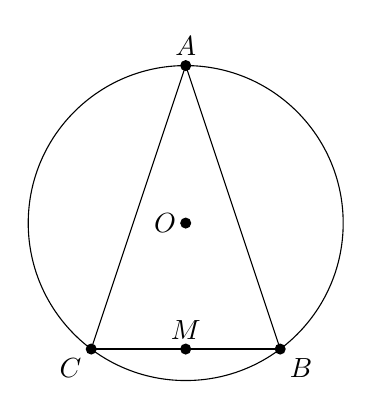
\begin{tikzpicture}[scale=2]
            \draw (0,0) circle (1);

            \node at (0,0) [left] {$O$};
            \fill (0,0) circle(1pt);
            \node at (0,1) [above] {$A$};
            \fill (0,1) circle(1pt);
            \node at (-0.6,-0.8) [below left] {$C$};
            \fill (-0.6,-0.8) circle(1pt);
            \node at (0.6,-0.8) [below right] {$B$};
            \fill (0.6,-0.8) circle(1pt);
            \node at (0,-0.8) [above] {$M$};
            \fill (0,-0.8) circle(1pt);

            \draw (0,1) -- (-0.6,-0.8);
            \draw (0,1) -- (0.6,-0.8);
            \draw (-0.6,-0.8) -- (0.6,-0.8);
            \end{tikzpicture}
        \end{center}

        设$\angle AOC=\theta$,这里$\theta\in(0,\pi)$,则可发现$\angle MOC=\pi-\theta$,从而底面半径$|MC|=a\sin\theta$,高$|AM|=a(1-\cos\theta)$\ (注意无论$\theta$是否大于$\frac{\pi}{2}$此式均正确),由此得圆锥体积
        $$V(\theta)=\frac{1}{3}\pi a^2\sin^2\theta\cdot a(1-\cos\theta)=\frac{\pi a^3}{3}\sin^2\theta(1-\cos\theta)$$
        记$t=\cos\theta$,其取值范围为$[-1,1]$,由$\sin^2\theta=1-\cos^2\theta$可发现只需考虑
        $$f(t)=(1-t^2)(1-t)$$
        何时取到最大值。直接求导得$f'(t)=(3t+1)(t-1)$,再结合取值范围,对比$-1$、$\frac{1}{3}$、1三点可发现$t=-\frac{1}{3}$时$f(t)$取到最大值$\frac{32}{27}$。
        
        由此,最终可得$|MC|=\frac{2\sqrt2}{3}a$、$|AM|=\frac{4}{3}a$时,圆锥体积取到最大值$\frac{32\pi}{81}a^3$。
    }

    \item (习题4.5.9)在曲线$y^2=4x$上求与$(18,0)$距离最近的点。
    
    \sol{
        设曲线上一点$(\frac{y^2}{4},y)$,则它到$(18,0)$的距离为
        $$d(y)=\sqrt{\bigg(18-\frac{y^2}{4}\bigg)^2+y^2}$$
        将$y^2$看成整体直接配方可得
        $$d(y)=\sqrt{\bigg(\frac{y^2}{4}-16\bigg)^2+68}$$
        从而利用二次函数知识可发现$d(y)$最小当且仅当$y^2=64$,即$y=\pm8$。由此,曲线上与$(18,0)$距离最近的点为$(16,\pm8)$,此时距离为$2\sqrt{17}$。

        \note 有时对于一些形式简单的函数,\textbf{观察化简}或许可以比求导更加简便。
    }

    \item (4.6节例1)设函数$f(x)=ax^3+bx^2+cx+d$,其中$a>0$,研究其凹凸性区间。
    
    \sol{
        直接计算可知$f''(x)=6ax+2b$,由条件可直接得到其在$(-\infty,-\frac{b}{3a})$为负,$(-\frac{b}{3a},+\infty)$为正,从而$x\in(-\infty,-\frac{b}{3a})$时$f(x)$向上凸,$x\in(-\frac{b}{3a},+\infty)$时$f(x)$向下凸。
    }

    \item (4.6节例3)画出函数$f(x)=\frac{x^2}{x-1}$的草图。
    
    \sol{
        \note 这类问题考试中不会出现,一般来说,研究函数时画怎样的草图取决于\textbf{想研究怎样的性质},如研究凹凸性需计算二阶导后画草图,而研究无穷远处性质则需计算渐近线。

        这里直接作出草图如下:
        \begin{center}  
            \begin{tikzpicture}[scale=0.5]
            \draw[->] (-3,0) -- (6,0) node[right] {$x$};
            \draw[->] (0,-3) -- (0,8) node[above] {$y$};

            \node at (0,0) [above right] {$O$};
            \fill (0,0) circle(2pt);
            \node at (0,2) [left] {2};
            \fill (0,2) circle(2pt);
            \node at (0,4) [left] {4};
            \fill (0,4) circle(2pt);
            \node at (0,6) [left] {6};
            \fill (0,6) circle(2pt);
            \node at (0,-2) [left] {$-2$};
            \fill (0,-2) circle(2pt);
            \node at (2,0) [below] {2};
            \fill (2,0) circle(2pt);
            \node at (4,0) [below] {4};
            \fill (4,0) circle(2pt);
            \node at (-2,0) [below] {$-2$};
            \fill (-2,0) circle(2pt);

            \draw[domain=-3:0.8,samples=20,smooth,thick,black]
            plot (\x,{\x+1+1/(\x-1)});
            \draw[domain=1.2:6,samples=20,smooth,thick,black]
            plot (\x,{\x+1+1/(\x-1)});
            \end{tikzpicture}
        \end{center}
    }

    \item (习题4.6.3)设函数$f(x)$在$(a,b)$有二阶导数,且向上凸,证明
    $$\forall x\in(a,b),\quad f''(x)\le0$$

    \sol{
        我们给出几种不同的方法:
        \begin{itemize}
            \item \textbf{零阶条件出发}
            
            我们先证明向上凸的函数的重要性质(称为向上凸的函数的\textbf{零阶条件}):
            $$\forall x,y\in(a,b),\quad\forall\lambda\in[0,1],\quad f(\lambda x+(1-\lambda)y)\ge\lambda f(x)+(1-\lambda)f(y)$$

            设$z=\lambda x+(1-\lambda)y$,若$x=y$或$\lambda=0$或$\lambda=1$可发现结论已经成立,其他情况$z\ne x$且$z\ne y$,直接利用条件可知
            $$f(x)<f(z)+f'(z)(x-z),\quad f(y)<f(z)+f'(z)(y-z)$$
            也即
            $$f(x)<f(z)+f'(z)(1-\lambda)(x-y),\quad f(y)<f(z)+f'(z)\lambda(y-x)$$
            由$\lambda\in[0,1]$,第一式乘$\lambda$加第二式乘$1-\lambda$即得结论。

            由此,对任何$x_0\in(a,b)$与满足$x_0\pm h\in(a,b)$的实数$h$,在零阶条件中代入$x=x_0+h$、$y=x_0-h$、$\lambda=\frac{1}{2}$,有
            $$f(x_0+h)+f(x_0-h)\le2f(x_0)$$
            从而可知$h\ne0$时
            $$\frac{f(x_0+h)+f(x_0-h)-2f(x_0)}{h^2}\le0$$
            由$f$二阶导存在,验证条件并利用洛必达法则可发现
            $$\lim_{h\to0}\frac{f(x_0+h)+f(x_0-h)-2f(x_0)}{h^2}=\lim_{h\to0}\frac{f'(x_0+h)-f'(x_0-h)}{2h}=f''(x_0)$$
            从而由极限保序性即得$f''(x_0)\le0$。

            \note 这里最后一个等号类似\exref{deri multi},注意\textbf{无法再次使用洛必达法则},因为再次使用洛必达法则将得到$\frac{f''(x_0+h)+f''(x_0-h)}{2}$,在二阶导函数未必连续的情况下它的极限未必与$f''(x_0)$相等。

            \item \textbf{一阶条件出发}
            
            任取$x_0\in(a,b)$,再取$x\ne x_0$且$x\in(a,b)$,有
            $$f(x)<f(x_0)+f'(x_0)(x-x_0)$$
            另一方面也有
            $$f(x_0)<f(x)+f'(x)(x_0-x)$$
            两式相加并消去$f(x)+f(x_0)$即得
            $$0<(f'(x_0)-f'(x))(x-x_0)$$
            除以$(x_0-x)^2$并整理得到
            $$\frac{f'(x)-f'(x_0)}{x-x_0}<0$$
            于是利用二阶导数定义与极限保序性有
            $$f''(x_0)=\lim_{x\to x_0}\frac{f'(x)-f'(x_0)}{x-x_0}\le0$$
            这就得到了证明。

            \item \textbf{微分中值定理}

            任取$x_0\in(a,b)$,再取$x>x_0$且$x\in(a,b)$,有
            $$f(x)<f(x_0)+f'(x_0)(x-x_0)$$
            同除以$x-x_0$即得$x>x_0$时
            $$f'(x_0)>\frac{f(x)-f(x_0)}{x-x_0}$$
            由拉格朗日中值定理,存在$\xi\in(x_0,x)$\ (记为$\xi(x)$)使得右侧为$f'(\xi)$,从而得到
            $$f'(x_0)>f'(\xi(x))$$
            由$\xi$范围可知$\xi(x)>x_0$,于是
            $$\frac{f'(\xi(x))-f'(x_0)}{\xi(x)-x_0}<0$$
            同理可发现,$x<x_0$时上式也成立,从而对任何$x\ne x_0$,存在$x_0$与$x$之间的$\xi(x)$使得上式成立。接下来考虑
            $$\lim_{x\to x_0}\frac{f'(\xi(x))-f'(x_0)}{\xi(x)-x_0}$$
            利用夹逼定理可得$x\to x_0$时$\xi(x)\to x_0$。由于$\xi(x)$在$x\ne x_0$时恒不为$x_0$,利用\textbf{推广的复合函数极限}(\exref{comb extra}中的第二种情况,此结论教材上没有,不过可以直接使用)与极限保序性即可得到
            $$0\ge\lim_{x\to x_0}\frac{f'(\xi(x))-f'(x_0)}{\xi(x)-x_0}=\lim_{\xi\to x_0}\frac{f'(\xi)-f'(x_0)}{\xi-x_0}=f''(x_0)$$
            这就得到了证明。

            \note 若不想直接使用推广的复合函数极限结论,就需要与本讲义11.1第6题相同讨论了。
        \end{itemize}

        \note 将教材上定义中的小于号改为小于等于号,我们就得到了\textbf{向上非严格凸}(类似非严格单调)的定义。本题结论对于向上非严格凸的函数仍然成立,可与上方完全类似证明。

        \note 本题的经典错误是使用\textbf{带二阶拉格朗日余项的泰勒展开}。展开可以得到对任何满足$x\in(a,b)$、$x+h\in(a,b)$,存在$x$与$x+h$之间的$\xi$使得$f(x+h)=f(x)+hf'(x)+\frac{h^2}{2}f''(\xi)$,从而结合定义知$f''(\xi)>0$。但是,由于\textbf{二阶导函数未必连续},即使$h\to0$时$\xi\to x$也无法保证$f''(\xi)$趋于$f''(x)$;另一方面,我们同样无法保证对任何$\xi$都存在$x$与$x+h$使得的确能在余项中取到$\xi$——事实上的确可能无法找到$x$与$x+h$。
    }

    \item (5.1节例)设四边形$ABCD$中$E$、$F$是边$AB$、$CD$的中点,$G$、$H$是对角线$AC$、$BD$的中点,求证:
    \begin{enumerate}[(1)]
        \item $\overrightarrow{AD}+\overrightarrow{BC}=2\overrightarrow{EF}$
        
        \sol{
            为了从右配凑出左,我们利用两种展开方式可发现
            $$\overrightarrow{EF}=\overrightarrow{EA}+\overrightarrow{AD}+\overrightarrow{DF}$$
            $$\overrightarrow{EF}=\overrightarrow{EB}+\overrightarrow{BC}+\overrightarrow{CF}$$
            由中点定义可知$\overrightarrow{EA}+\overrightarrow{EB}=\overrightarrow{DF}+\overrightarrow{CF}=\bm{0}$,从而两式相加得结论。

            \note 可以发现,利用向量我们可以做到纯\textbf{代数化}解决几何问题,无需再画出图形。
        }

        \item $\overrightarrow{AB}+\overrightarrow{AD}+\overrightarrow{CB}+\overrightarrow{CD}=4\overrightarrow{GH}$

        \sol{
            与(1)类似,为了配凑写出四种展开
            $$\overrightarrow{GH}=\overrightarrow{GA}+\overrightarrow{AB}+\overrightarrow{BH}$$
            $$\overrightarrow{GH}=\overrightarrow{GA}+\overrightarrow{AD}+\overrightarrow{DH}$$
            $$\overrightarrow{GH}=\overrightarrow{GC}+\overrightarrow{CB}+\overrightarrow{BH}$$
            $$\overrightarrow{GH}=\overrightarrow{GA}+\overrightarrow{CD}+\overrightarrow{DH}$$
            由中点定义可知$\overrightarrow{GA}+\overrightarrow{GC}=\overrightarrow{BH}+\overrightarrow{DH}=\bm{0}$,从而四式相加得结论。
        }
    \end{enumerate}

    \note 从证明中可以看出本题两问的结论都\textbf{无需$ABCD$构成平面四边形},在空间中任取四个点均成立上述性质。

    \item (习题5.1.1)设平行四边形$ABCD$中$\overrightarrow{AB}=\bm{a}$、$\overrightarrow{AD}=\bm{b}$,用$\bm{a}$、$\bm{b}$表示向量$\overrightarrow{AC}$、$\overrightarrow{DB}$、$\overrightarrow{MA}$,其中$M$为对角线交点。
    
    \sol{
        直接利用平行性可知$\overrightarrow{AB}=\overrightarrow{DC}$、$\overrightarrow{AD}=\overrightarrow{BC}$,由此
        $$\overrightarrow{AC}=\overrightarrow{AB}+\overrightarrow{BC}=\bm{a}+\bm{b}$$
        $$\overrightarrow{DB}=\overrightarrow{DA}+\overrightarrow{AB}=\bm{a}-\bm{b}$$
        由$M$为对角线$AC$的中点可知
        $$\overrightarrow{MA}=\frac{1}{2}\overrightarrow{CA}=-\frac{1}{2}\overrightarrow{AC}=-\frac{1}{2}\bm{a}-\frac{1}{2}\bm{b}$$
    }

    \item (习题5.1.3)设$M$为三角形$ABC$的重心,$O$为空间中任何一点,证明
    $$\overrightarrow{OM}=\frac{1}{3}\big(\overrightarrow{OA}+\overrightarrow{OB}+\overrightarrow{OC}\big)$$

    \sol{
        两侧同加$\overrightarrow{MO}$可发现等价于要证
        $$\frac{1}{3}\big(\overrightarrow{MA}+\overrightarrow{MB}+\overrightarrow{MC}\big)=\bm{0}$$
        两侧同乘$-3$也即
        $$\overrightarrow{AM}+\overrightarrow{BM}+\overrightarrow{CM}=\bm{0}$$
        由于已知$M$为三条中线的交点,设$AB$、$AC$中点为$D$、$F$,则有
        $$\overrightarrow{AD}=\frac{1}{2}\overrightarrow{AB}$$
        $$\overrightarrow{AF}=\frac{1}{2}\overrightarrow{AC}$$
        设
        $$\overrightarrow{AM}=\lambda\overrightarrow{AB}+\mu\overrightarrow{AC}$$
        由于$B$、$M$、$F$共线可知$\overrightarrow{BM}$与$\overrightarrow{BF}$成比例,由它们均非零向量可知存在$k_1$使得
        $$(\lambda-1)\overrightarrow{AB}+\mu\overrightarrow{AC}=\overrightarrow{AM}-\overrightarrow{AB}=\overrightarrow{BM}=k_1\overrightarrow{BF}=k_1(\overrightarrow{AF}-\overrightarrow{AB})=-k_1\overrightarrow{AB}+\frac{k_1}{2}\overrightarrow{AC}$$
        同理考虑$C$、$M$、$D$可知存在$k_2$使得
        $$\lambda\overrightarrow{AB}+(\mu-1)\overrightarrow{AC}=\frac{k_2}{2}\overrightarrow{AB}-k_2\overrightarrow{AC}$$
        由于$\overrightarrow{AB}$、$\overrightarrow{AC}$不共线,必然有
        $$\lambda-1=-k_1,\quad\mu=\frac{k_1}{2},\quad\lambda=\frac{k_2}{2},\quad\mu-1=-k_2$$
        由此联立可解出
        $$\lambda=\mu=\frac{1}{3}$$
        也即
        $$\overrightarrow{AM}=\frac{1}{3}\overrightarrow{AB}+\frac{1}{3}\overrightarrow{AC}$$
        同理
        $$\overrightarrow{BM}=\frac{1}{3}\overrightarrow{BA}+\frac{1}{3}\overrightarrow{BC}$$
        $$\overrightarrow{CM}=\frac{1}{3}\overrightarrow{CA}+\frac{1}{3}\overrightarrow{CB}$$
        三式求和,由右侧互相抵消可知为0,从而得证。

        \note 本题也可以从几何出发利用倍长中线技巧计算,虽然更加简单,但更\textbf{依赖思考},这里主要介绍基于向量代数的证明方法。
    }

    \item (习题5.1.7)利用向量证明:
    \begin{enumerate}[(1)]
        \item 菱形的对角线互相垂直,且平分顶角。
        
        \sol{
            考虑菱形$ABCD$,对角线为$AC$与$BD$,有
            $$\overrightarrow{AC}\cdot\overrightarrow{BD}=(\overrightarrow{AB}+\overrightarrow{BC})\cdot(\overrightarrow{BC}+\overrightarrow{CD})=\overrightarrow{AB}\cdot\overrightarrow{BC}+\overrightarrow{AB}\cdot\overrightarrow{CD}+\overrightarrow{BC}\cdot\overrightarrow{BC}+\overrightarrow{BC}\cdot\overrightarrow{CD}$$
            最后一步展开利用了内积的分配律。由菱形为平行四边形可知$\overrightarrow{AB}=\overrightarrow{DC}$、$\overrightarrow{AD}=\overrightarrow{BC}$,进一步利用$|\vec{x}|^2=\vec{x}\cdot\vec{x}$与菱形邻边相等可知上式为
            $$\overrightarrow{AB}\cdot\overrightarrow{AD}-|\overrightarrow{AB}|^2+|\overrightarrow{AD}|^2-\overrightarrow{AD}\cdot\overrightarrow{AB}=|\overrightarrow{AD}|^2-|\overrightarrow{AB}|^2=0$$
            这就得到了$\overrightarrow{AC}\cdot\overrightarrow{BD}=0$,于是对角线垂直。

            进一步地,从上式可以推出
            $$\overrightarrow{AC}\cdot(\overrightarrow{BC}+\overrightarrow{CD})=0$$
            于是移项整理得到
            $$\overrightarrow{AC}\cdot\overrightarrow{BC}=\overrightarrow{AC}\cdot\overrightarrow{DC}$$
            由菱形性质$|\overrightarrow{BC}|=|\overrightarrow{DC}|$,两侧同除以$|\overrightarrow{AC}||\overrightarrow{BC}|$即得
            $$\cos\angle CAB=\cos\angle CAD$$
            由几何关系可知必须$\angle CAB=\angle CAD$,这即代表$AC$平分$\angle BAD$,同理$AC$也平分$\angle BCD$,$BD$平分$\angle ABC$、$\angle ADC$,这即代表对角线平分顶角。
        }

        \item 勾股定理。
        
        \sol{
            考虑直角三角形$ABC$,其中$\angle ABC=\frac{\pi}{2}$,则有
            $$|\overrightarrow{AC}|^2=|\overrightarrow{AB}+\overrightarrow{BC}|^2=\overrightarrow{AB}\cdot \overrightarrow{AB}+\overrightarrow{BC}\cdot\overrightarrow{BC}+2\overrightarrow{AB}\cdot \overrightarrow{BC}=|\overrightarrow{AB}|^2+|\overrightarrow{BC}|^2$$
            从而得证。中间的展开利用了$|\vec{x}|^2=\vec{x}\cdot\vec{x}$与内积的\textbf{线性性}(即对数乘的结合律、分配律)与\textbf{对称性}(即交换律)。
        }
    \end{enumerate}

    \item (习题5.1.8)对于任意两个向量$\bm{a}$、$\bm{b}$,证明
    $$|\bm{a}\times\bm{b}|^2+(\bm{a}\cdot\bm{b})^2=|\bm{a}|^2|\bm{b}|^2$$

    \sol{
        直接利用定义可知
        $$|\bm{a}\times\bm{b}|^2+(\bm{a}\cdot\bm{b})^2=|\bm{a}|^2|\bm{b}|^2\sin^2\theta+|\bm{a}|^2|\bm{b}|^2\cos^2\theta=|\bm{a}|^2|\bm{b}|^2$$
        这里$\theta$为$\bm{a}$、$\bm{b}$夹角。
    }
\end{enumerate}

\subsection{根与存在性}
\subsubsection{多项式的根}
微分中值定理的一个重要应用是判断函数的\textbf{根}的情况。一方面,罗尔中值定理代表着$f(x)$的两个根之间必然存在$f'(x)$的一个根;另一方面,通过微分中值定理证明的\textbf{单调性}又可以确定某个范围内根不会更多。

本节中,我们默认\textbf{代数学基本定理}成立,也即对$n$次多项式$f$,一定存在$n$个复数$c_1,\dots,c_n$使得$f(x)=(x-c_1)\dots(x-c_n)$。

先来看两个找根相关的问题:

\begin{framed}
\begin{exercise}\label{deri n xx}
    对正整数$n$,证明
    $$P(x)=\frac{1}{2^nn!}\frac{\dr^n}{\dr x^n}(x^2-1)^n$$
    在$(-1,1)$有$n$个不同实根。
\end{exercise}
\sol{
    可忽略不会为0的常数,记$f(x)=(x^2-1)^n$,我们先进行\textbf{观察},再\textbf{归纳}证明:
    \begin{itemize}
        \item \textbf{观察与尝试}

        首先,由于$f(x)$是一个$2n$次多项式,求$n$阶导后应当为$n$次多项式,利用代数学基本定理,只要找到了$(-1,1)$上的$n$个不同实根(也即说明$P(x)$在$(-1,1)$\textbf{至少}有$n$个根),即能说明它们是$P(x)$的全部实根,从而得证。

        为了证明$f(x)$的$n$阶导数有$n$个根,我们先对原函数与导函数进行观察:$f(x)$有1、$-1$两个根,从而利用罗尔中值定理存在$\xi\in(-1,1)$使得$f'(x)=0$\ (实际上计算可得$\xi=0$)。若$n=1$已经得证,其他情况下,由于
        $$f'(x)=2nx(x^2-1)^{n-1}$$
        仍然以$-1$、1为根,这就得到了$f'(x)$的三个根。进一步地,从$f'(x)$的$-1$、$\xi$、1三个根可以得到$\xi_1\in(-1,\xi)$、$\xi_2\in(\xi,1)$两个根,若$n=2$已经得证。
        
        否则,可以发现$f''$也以$\pm1$为根,以此循环,每多求一阶导会增加一个根,直到最终得到$n$个根。

        \item \textbf{归纳多项式性质}

        我们先证明,对任何$k=0,\dots,n$,存在多项式$p_k(x)$使得
        $$f^{(k)}(x)=p_k(x)(x^2-1)^{n-k}$$
        直接归纳:当$k=0$时结论成立,若结论对$k-1$成立,考虑$k$的情况($1\le k\le n$)可知
        $$\begin{aligned}f^{(k)}(x)&=\frac{\dr}{\dr x}p_{k-1}(x)(x^2-1)^{n-k+1}\\ &=p_{k-1}'(x)(x^2-1)^{n-k+1}+2(n-k+1)xp_{k-1}(x)(x^2-1)^{n-k}\\ &=(2(n-k+1)xp_{k-1}(x)+(x^2-1)p_{k-1}'(x))(x^2-1)^{n-k}\end{aligned}$$
        这就得到了证明。

        \item \textbf{归纳根的情况}

        我们已经证明了对$k=0,1,\dots,n-1$,$f^{(k)}(x)$都以$x=\pm1$为根,接下来只需要进一步归纳说明,对$k=0,\dots,n$,$f^{(k)}(x)$\textbf{至少}有$k$个在$(-1,1)$中的根:

        当$k=0$时结论成立,若结论对$k-1$成立,考虑$k$的情况($1\le k\le n$),设$f^{(k-1)}(x)$在$(-1,1)$中的$k-1$个不同根为
        $$-1<\eta_1<\eta_2<\dots<\eta_{k-1}<1$$
        由$k$的范围,$f^{(k-1)}(x)$以$-1$、1为根,从而
        $$f^{(k-1)}(-1)=f^{(k-1)}(\eta_1)=f^{(k-1)}(\eta_2)=\dots=f^{(k-1)}(\eta_{k-1})=f^{(k-1)}(1)=0$$
        利用罗尔中值定理即得存在
        $$\xi_1\in(-1,\eta_1),\quad\xi_2\in(\eta_1,\eta_2),\quad\dots,\quad\xi_k\in(\eta_{k-1},1)$$
        使得
        $$f^{(k)}(\xi_1)=f^{(k)}(\xi_2)=\dots=f^{(k)}(\xi_k)=0$$
        从而得证。

        由此,$f^{(n)}(x)$至少有$n$个在$(-1,1)$中的根,利用代数学基本定理知其至多$n$个根,从而恰有$n$个在$(-1,1)$中的根,结论成立。
    \end{itemize}
}
\end{framed}

\begin{framed}
\begin{exercise}[\extra]\label{deri n ex}
    证明
    $$C(x)=\er^x\frac{\dr^n}{\dr x^n}(x^n\er^{-x})$$
    有$n$个不同的正实根。
\end{exercise}
\sol{
    可忽略不会为0的$\er^x$部分,记$f(x)=x^n\er{-x}$,我们先进行\textbf{观察},再\textbf{归纳}证明:
    \begin{itemize}
        \item \textbf{观察与尝试}
        
        简单计算可以发现,对任何自然数$k$,$f^{(k)}(x)$都是一个$x$的$n$次多项式乘$\er^{-x}$,从而$C(x)$是$x$的$n$次多项式,利用代数学基本定理,只要证明$C(x)$\textbf{至少}有$n$个不同正实根即可。

        类似\exref{deri n xx}进行分析,可以发现对$0\le k\le n-1$,0都必然是$f^{(k)}(x)$的解,但我们必须找到\textbf{另一个解}才能让根的个数不断增加。尝试计算几次$f^{(k)}(x)$可发现,对$0\le k\le n-1$,$f^{(k)}(x)$有$k+1$个不同的解
        $$0<x_1<x_2<x_3<\dots<x_k$$
        而$f^{(k+1)}(x)$的正根$y_1,\dots,y_{k+1}$满足
        $$y_1\in(0,x_1),\quad y_2\in(x_1,x_2),\quad\dots,\quad y_k\in(x_{k-1},x_k),\quad y_{k+1}>x_k$$
        由于新增了更大的根,我们可以考虑\textbf{无穷}处:利用指数函数的性质可知
        $$\lim_{x\to+\infty}f^{(k)}(x)=0$$
        由此$+\infty$可以某种意义上看作$f^{(k)}(x)$的根。如果我们真的能说明$x_k$与$+\infty$之间存在$f^{(k+1)(x)}$的根,证明就已经完成了。由此,我们想到如下先\textbf{推广中值定理}再归纳的过程。

        \item \textbf{微分中值引理}
        
        我们先证明引理,若$\rb$上可导的函数$g(x)$满足
        $$g(x_0)=0,\quad\lim_{x\to+\infty}g(x)=0$$
        则存在$\xi>x_0$使得$g'(\xi)=0$。

        利用微分中值定理,只要$g(x)$在$x\ge x_0$的两个不同点处值相等,即能得到符合要求的$\xi$。若不存在,由$g$的连续性,完全类似\exref{cont inj mono}可证明$g$是\textbf{严格单调}的,不妨设$g$严格单调增(若严格单调减,类似证明即可),则$g(x_0+1)>g(x_0)=0$,又由极限\textbf{保序性}即得
        $$\lim_{x\to+\infty}g(x)\ge g(x_0+1)>0$$
        从而矛盾。若$g$严格单调减,类似可证明矛盾,综合即知引理成立。
        
        \item \textbf{归纳多项式性质}
        
        我们先证明,对任何$k=0,\dots,n$,存在多项式$p_k(x)$使得
        $$f^{(k)}(x)=p_k(x)x^{n-k}\er^{-x}$$
        直接归纳:当$k=0$时结论成立,若结论对$k-1$成立,考虑$k$的情况$(1\le k\le n)$可知
        $$\begin{aligned}f^{(k)}(x)&=\frac{\dr}{\dr x}p_{k-1}(x)x^{n-k+1}\er^{-x}\\ &=p_{k-1}'(x)x^{n-k+1}\er^{-x}+(n-k+1)p_{k-1}(x)x^{n-k}\er^{-x}-p_{k-1}(x)x^{n-k+1}\er^{-x}\\ &=(xp_{k-1}'(x)+(n-k+1)p_{k_1}(x)-xp_{k-1}(x))x^{n-k}\er^{-x}\end{aligned}$$
        这就得到了证明
        
        \item \textbf{归纳根的情况}
        
        我们已经证明了对$k=0,1,\dots,n-1$,$f^{(k)}(x)$都以$x=0$为根,接下来只需要进一步归纳说明,对$k=0,\dots,n$,$f^{(k)}(x)$\textbf{至少}有$k$个在$(0,+\infty)$中的根:

        当$k=0$时结论成立,若结论对$k-1$成立,考虑$k$的情况($1\le k\le n$),设$f^{(k-1)}(x)$在$(0,+\infty)$中的$k-1$个不同根为
        $$0<\eta_1<\eta_2<\dots<\eta_{k-1}$$
        由$k$的范围,$f^{(k-1)}(x)$以0为根,从而
        $$f^{(k-1)}(0)=f^{(k-1)}(\eta_1)=\dots=f^{(k-1)}(\eta_{k-1})=0$$
        利用罗尔中值定理即得存在
        $$\xi_1\in(0,\eta_1),\quad\xi_2\in(\eta_1,\eta_2),\quad\dots,\quad\xi_{k-1}\in(\eta_{k-2},\eta_{k-1})$$
        使得
        $$f^{(k)}(\xi_1)=f^{(k)}(\xi_2)=\dots=f^{(k)}(\xi_{k-1})=0$$
        此外,利用\exref{func other ord}的结论可知
        $$\lim_{x\to+\infty}f^{(k-1)}(x)=0$$
        于是由引理存在$\xi_k>\eta_{k-1}$使得$f^{(k)}(\xi_k)=0$,从而得证。

        由此,$f^{(n)}(x)$至少有$n$个在$(0,+\infty)$中的根,利用代数学基本定理知其至多$n$个根,从而恰有$n$个在$(0,+\infty)$中的根,结论成立。
    \end{itemize}
}
\end{framed}

对于更一般的情况,我们还可以结合介值定理、单调性等来确定根的\textbf{具体个数}:
\begin{framed}
\begin{exercise}
    对正整数$n$,设函数
    $$f(x)=1-x+\frac{x^2}{2}-\dots+(-1)^n\frac{x^n}{n}$$
    证明$f(x)=0$在$n$为奇数时有一个实根,$n$为偶数时无实根。
\end{exercise}
\sol{
    直接利用等比数列求和可知$x\ne-1$时
    $$f'(x)=0-1+x-\dots+(-1)^nx^{n-1}=\frac{(-x)^n-1}{1+x}$$
    而$x=-1$时代入计算得$f'(x)=-n$。

    分类讨论:
    \begin{itemize}
        \item 当$n$为奇数时
        $$f'(x)=\begin{cases}\frac{-x^n-1}{1+x}&x\ne-1\\-n&x=-1\end{cases}$$
        当$x>-1$时分母为正、分子为负,当$x<-1$时分子为正、分母为负,从而$f'(x)$恒小于0,这就得到$f'(x)$在$\rb$上\textbf{严格单调减},至多有一个实根。

        利用本讲义6.1第6题结论(此结论可直接使用)可得$f(x)$必然有一个实根,从而恰有一个实根。

        \item 当$n$为偶数时
        $$f'(x)=\begin{cases}\frac{x^n-1}{1+x}&x\ne-1\\-n&x=-1\end{cases}$$
        当$x<-1$时分子为正、分母为负,当$x\in(-1,1)$时分子为负、分母为正,当$x>1$时分子分母都为正,综合可得$f'(x)$在$(-\infty,1)$为负,在$(1,+\infty)$为正。

        由此,$f'(x)$在$(-\infty,1]$严格单调减,在$[1,+\infty)$严格单调增,因此1处取到最小值,而$n$为偶数时
        $$f(1)=1-1+\frac{1}{2}-\frac{1}{3}+\dots-\frac{1}{n-1}+\frac{1}{n}=(1-1)+\bigg(\frac{1}{2}-\frac{1}{3}\bigg)+\dots+\bigg(\frac{1}{n-2}-\frac{1}{n-1}\bigg)+\frac{1}{n}>0$$
        由此可知$f(x)$恒大于0,无实根。
    \end{itemize}
}
\end{framed}
\begin{framed}
\begin{exercise}
    对$a<b$与正整数$n$,若$n$次多项式$P(x)$满足$P(x)-a$、$P(x)-b$都有$n$个不同实根,证明对$c\in(a,b)$,$P(x)-c$也有$n$个不同实根。
\end{exercise}
\sol{
    设$P(x)-a$的实根从小到大排列为$a_1,\dots,a_n$,$P(x)-b$的实根从小到大排列为$b_1,\dots,b_n$。

    由于$P(x)-a$有$n$个不同实根,利用罗尔中值定理,存在
    $$\xi_1\in(a_1,a_2),\quad\xi_2\in(b_1,b_2),\quad\dots,\quad\xi_{n-1}\in(a_{n-1},a_n)$$
    使得$P'(\xi_1)=P'(\xi_2)=\dots=P'(\xi_{n-1})=0$。

    由于$P(x)$为$n$次多项式,$P'(x)$为$n-1$次多项式,利用\textbf{代数学基本定理}知存在$t\ne0$使得
    $$P'(x)=t(x-\xi_1)(x-\xi_2)\dots(x-\xi_{n-1})$$
    由此,进一步观察可知$P'(x)$在以下$n$个区间:
    $$I_1=(-\infty,\xi_1),\quad I_2=(\xi_1,\xi_2),\quad\dots,\quad I_{n-1}=(\xi_{n-2},\xi_{n-1}),\quad I_n=(\xi_{n-1},+\infty)$$
    均\textbf{不变号},由此$P(x)$在
    $$J_1=(-\infty,\xi_1],\quad J_2=(\xi_1,\xi_2],\quad\dots,\quad J_{n-1}=(\xi_{n-2},\xi_{n-1}],\quad J_n=(\xi_{n-1},+\infty)$$
    均\textbf{严格单调}。

    利用严格单调性的定义,在每个$J_i$中,对任何$s\in\rb$,$P(x)=s$至多只有一个解,由此又由于$J_1$到$J_n$两两交为空且能\textbf{拼成}$\rb$,$P(x)=a$与$P(x)=b$在每个区间中都\textbf{恰有}一个解。于是
    $$a_k\in J_k,\quad b_k\in J_k$$
    根据\textbf{介值定理},存在$a_k$、$b_k$之间的$c_k$使得$F(c_k)=c$,由于$c_k\in J_k$,$c_1$到$c_n$必然满足
    $$c_1<c_2<\dots<c_n$$
    也即我们找到了$P(x)-c$的$n$个不同实根。再通过严格单调性,每个$J_k$中至多有一个实根,最终证明$P(x)=c$\textbf{恰有}$n$个不同实根,得证。

    \note 本题也可以先在\textbf{几何角度观察},进一步想到从单调区间的方向证明。
}
\end{framed}

\subsubsection{存在性问题}
除此以外,结合\textbf{构造函数}的中值定理可以解决更复杂的\textbf{存在性}问题,如下方从易到难的三道例题:
\begin{framed}
\begin{exercise}
    若$\rb$上可导的函数$f(x)$有$a$、$b$两个零点,证明方程
    $$f(x)+f'(x)=0$$
    在$(a,b)$至少有一个解。
\end{exercise}
\sol{
    设
    $$F(x)=\er^xf(x)$$
    则
    $$F'(a)=F'(b)=0,\quad F'(x)=(f(x)+f'(x))\er^x$$
    利用罗尔中值定理,存在$\xi\in(a,b)$使得$F'(\xi)=0$,由$\er^\xi\ne0$即得结论。

    \note 对于一般的含导数的中值类问题,常见做法是\textbf{配凑成导数后}利用微分中值定理证明。本题中可见,$af(x)+f'(x)$这类式子的常见配凑方法是乘\textbf{指数函数}$\er^{ax}$。
}
\end{framed}

\begin{framed}
\begin{exercise}
    若$f(x)$在$[a,b]$一阶可微,且$0\notin[a,b]$,证明存在$\xi\in(a,b)$使得
    $$f(\xi)-\xi f'(\xi)=\frac{af(b)-bf(a)}{a-b}$$
\end{exercise}
\sol{
    本题有两种观察思路:
    \begin{itemize}
        \item 式子左侧,$f'(\xi)$比$f(\xi)$多乘$\xi$,可以想到类似\textbf{幂函数}的形式,从而设$F(x)=x^kf(x)$可发现
        $$F'(x)=kx^{k-1}f(x)+x^kf'(x)=x^{k-1}(kf'(x)+xf(x))$$
        由此,取$k=-1$即发现
        $$F(x)=\frac{f(x)}{x},\quad f(\xi)-\xi f'(\xi)=-\xi^2F'(\xi)$$

        \item 式子右侧,我们尝试配凑成\textbf{柯西中值定理}$\frac{g(b)-g(a)}{h(b)-h(a)}$的形式,观察发现,只要分子分母同除以$ab$\ (由条件$ab\ne0$)就能得到
        $$\frac{\frac{f(b)}{b}-\frac{f(a)}{a}}{\frac{1}{b}-\frac{1}{a}}$$
    \end{itemize}
    无论从何种思路,我们最终令$F(x)=\frac{f(x)}{x}$,可发现目标式即为
    $$\frac{F(\xi)}{-\frac{1}{\xi^2}}=\frac{F(b)-F(a)}{\frac{1}{b}-\frac{1}{a}}$$
    记$G(x)=\frac{1}{x}$,由于$0\notin[a,b]$符合柯西中值定理条件,直接由柯西中值定理得结论成立。
}
\end{framed}

\begin{framed}
\begin{exercise}
    若$[a,b]$上二阶可微的函数$f(x)$满足$f(a)=f(b)=0$,证明对任何$x\in(a,b)$存在$\xi\in(a,b)$使得
    $$f(x)=\frac{f''(\xi)}{2}(x-a)(x-b)$$
\end{exercise}
\sol{
    考虑满足
    $$F''(t)=f(x)-\frac{f''(t)}{2}(x-a)(x-b)$$
    的函数$F(t)$,我们最终的目标为证明$F''(t)$在$(a,b)$存在零点,利用罗尔中值定理,需要找到$F(t)$的\textbf{三个零点}。
    
    由于第二项即为$\frac{f(t)}{2}(x-a)(x-b)$的二阶导数,利用原函数知识可知所有
    $$F(t)=\frac{f(x)}{2}p(t)-\frac{f(t)}{2}(x-a)(x-b)$$
    均符合要求,这里$p(t)=t^2+\alpha t+\beta$,$\alpha$、$\beta$可任取(一次函数求二阶导后直接为0)。

    由于前后的相似性质,我们\textbf{猜测}可以取$p(t)=(t-a)(t-b)$,对应的
    $$F(t)=\frac{f(x)}{2}(t-a)(t-b)-\frac{f(t)}{2}(x-a)(x-b)$$
    利用这样的$F(t)$构造,直接代入并使用条件$f(a)=f(b)=0$可知
    $$F(a)=F(x)=F(b)$$
    于是由罗尔中值定理
    $$\exists\xi_1\in(a,x),\quad\exists\xi_2\in(x,b),\quad F'(\xi)=F'(\xi_2)=0$$
    再由罗尔中值定理
    $$\exists\xi\in(\xi_1,\xi_2)\subset[a,b],\quad F''(\xi)=0$$
    代入$F''$的表达式可发现这就是符合要求的$\xi$。
}
\end{framed}

此外,存在性问题还可以和\textbf{极限}情况相结合:
\begin{framed}
\begin{exercise}
    若$\rb$上可导的函数$f(x)$满足
    $$\lim_{x\to+\infty}f(x)=\lim_{x\to-\infty}f(x)$$
    证明存在$\xi\in\rb$使得$f'(\xi)=0$。
\end{exercise}
\sol{
    \note 在\exref{deri n ex}的引理中,我们证明了类似的结论,此处将使用相同的思路。

    利用微分中值定理,只要$f(x)$在$\rb$上的两个不同点处值相等,即能得到符合要求的$\xi$。若不存在,由$f$的连续性,完全类似\exref{cont inj mono}可证明$f$是\textbf{严格单调}的,不妨设$f$严格单调增(若严格单调减,类似证明即可),则利用极限\textbf{保序性}可从
    $$\forall x>1,\quad f(x)>f(1)>f(0)>f(-1)>f(-x)$$
    取极限得到
    $$\lim_{x\to+\infty}f(x)\ge f(1)>f(0)>f(-1)\ge\lim_{x\to+\infty}f(-x)$$
    最后一个极限即$\lim_{x\to-\infty}f(x)$,从而与相等矛盾。
}
\end{framed}

\subsection{估算的方法}
\subsubsection{极限问题}
在学习完泰勒展开后,我们可以使用它进行函数性质的更充分刻画,从而解决更多的\textbf{估算}问题——当然,其中的有些问题事实上只需要微分中值定理就可以解决(对应\textbf{展开到一阶}),无需更复杂的研究。

首先是对极限的估算:
\begin{framed}
\begin{exercise}
    对$q\in[0,1)$,证明
    $$x_n=(1+q)(1+q^2)\dots(1+q^n)$$
    极限存在。
\end{exercise}
\sol{
    由于$x_n$每项都比前一项乘了大于1的数,它必然\textbf{单调增},且由定义有下界1,只需要再证明有上界。当$q=0$时,$x_n=1$符合要求,下面只考虑$q\in(0,1)$的情况。

    我们对连乘并无很好的处理方法,由此取\textbf{对数}得
    $$\ln x_n=\sum_{k=1}^n\ln(1+q^n)$$
    为了估算右侧,我们利用
    $$\lim_{n\to\infty}q^n=0,\quad\lim_{x\to0}\frac{\ln(1+x)}{x}=1$$
    由极限的\textbf{保序性},存在$\delta>0$使得
    $$\forall0<x<\delta,\quad\bigg|\frac{\ln(1+x)}{x}\bigg|<2$$
    而由极限定义可知
    $$\exists N,\quad\forall n>N,\quad|q^n|<\delta$$
    我们已经假设了$q\ne 0$,于是$0<q^n<\delta$,再结合$\ln(1+q^n)>0$可知$n>N$时
    $$\ln(1+q^n)<2q^n$$
    由此可知$n>N$时
    $$\ln x_n=\sum_{k=1}^N\ln(1+q^k)+\sum_{k=N}^n\ln(1+q^k)<\sum_{k=1}^N\ln(1+q^k)+\sum_{k=N}^n2q^k$$
    直接计算可知
    $$\sum_{k=N}^n2q^k<\sum_{k=0}^n2q^k=2\frac{1-q^{n+1}}{1-q}<\frac{2}{1-q}$$
    由此最终得到对任何$n>N$有
    $$\ln x_n<\sum_{k=1}^N\ln(1+q^k)+\frac{2}{1-q}$$
    利用$x_n$的单调增性质,上述不等式对$n\le N$也成立,这就证明了$x_n$有\textbf{上界},因此极限存在。

    \note 对本题来说,利用高中知识$\ln(1+x)<x$可以更快得到结果,但上面介绍的从\textbf{极限保序性出发的估算}是更加\textbf{通用}的估计方法,例如完全相同可以证明,只要$x\to0$时$f(x)\sim x$,所有$f(q^n)$的求和必然有界。
}
\end{framed}

\begin{framed}
\begin{exercise}
    若$\rb$上可导的函数$f(x)$满足
    $$\lim_{x\to+\infty}f'(x)=0$$
    证明
    $$\lim_{x\to+\infty}\frac{f(x)}{x}=0$$
\end{exercise}
\sol{
    \note 注意本题\textbf{无法直接使用洛必达法则},因为$f(x)$在$x\to+\infty$的情况是未知的。

    此处我们将介绍如何把期中前常用的\textbf{分段估算}技巧与中值定理结合,先分析再求解:
    \begin{itemize}
        \item \textbf{分析}
        
        从直观来看,如果$f'(x)$\textbf{连续},我们就能把$f(x)$看作$f'(x)$的积分,而$\frac{f(x)}{x}$就是$f'$在0到$x$的``高度平均''。由于$f'$的极限为0,高度的平均也将逐渐降低到0。

        虽然$f'$并不一定连续,根据之前所说的\textbf{导函数是连续函数推广}的思路,我们应当仍然可以类似拆分估算。在$f'$连续时,我们会将积分拆分为$|f'|$充分小与$|f'|$充分小之前两部分,此思路是可以保留的。

        \item \textbf{求解}
        
        由极限定义对任何$\varepsilon>0$,存在$M>0$使得
        $$\forall x>M,\quad|f'(x)|<\varepsilon$$
        从而对$x>M$,由\textbf{拉格朗日中值定理}存在$\xi\in(M,x)$使得
        $$\frac{f(x)}{x}=\frac{f(x)-f(M)}{x}+\frac{f(M)}{x}=\frac{f'(\xi)(x-M)}{x}+\frac{f(M)}{x}$$
        由此通过三角不等式即得$x>M$时(由$M>0$可知$x>0$)
        $$\bigg|\frac{f(x)}{x}\bigg|<\varepsilon\bigg(1-\frac{M}{x}\bigg)+\frac{|f(M)|}{x}$$
        由于右侧在$x\to+\infty$时极限为$\varepsilon$,利用极限\textbf{保序性}得存在$M_1>0$使得
        $$\forall x>M_1,\quad \varepsilon\bigg(1-\frac{M}{x}\bigg)+\frac{|f(M)|}{x}<2\varepsilon$$
        此时
        $$\bigg|\frac{f(x)}{x}\bigg|<2\varepsilon$$
        由于对任何$\varepsilon>0$都可以找到$M_1>0$使得$x>M_1$时上式成立,根据极限定义得证。
    \end{itemize}
}
\end{framed}

除了显式出现极限的问题,出现\textbf{积分}或\textbf{不等式控制出等式}类问题,也可能会用到极限的思想:
\begin{framed}
\begin{exercise}\label{deri inte not cont}
    若$[a,b]$上一阶可微的函数$F(x)$满足导函数$F'(x)$在$[a,b]$可积(由于有限个点不影响可积性,端点处可任意定义$F'$),证明
    $$\int_a^bF'(x)\dr x=F(b)-F(a)$$
\end{exercise}
\sol{
    \begin{itemize}
        \item \textbf{分析}
        
        本题的条件只有可积,而我们几乎没有学过除了\textbf{定义}以外应用此条件的方式,由此想到需要使用定义。

        设左侧积分为$A$,根据定义可知,对划分$T\colon a=x_0<x_1<\dots<x_n=b$,取任意分点$\xi_i\in[x_{i-1},x_i]$\ ($i=1,\dots,n$),设$\lambda(T)$为$T$最长分段的长度,有
        $$A=\lim_{\lambda(T)\to0^+}\sum_{k=1}^nF'(\xi_k)(x_k-x_{k-1})$$
        可以发现,此形式\textbf{非常接近}微分中值定理,从而可得证明思路。

        \item \textbf{求解}
        
        仍设左侧积分为$A$。对任何划分$T\colon a=x_0<x_1<\dots<x_n=b$,由拉格朗日中值定理,存在$\xi_i\in(x_{i-1},x_i)$\ ($i=1,\dots,n$),使得
        $$F(b)-F(a)=\sum_{k=1}^n(F(x_k)-F(x_{k-1}))=\sum_{k=1}^nF'(\xi_k)(x_k-x_{k-1})$$
        由于可积性,在$T$中任意取分点$\xi_1,\dots,\xi_n$,在$\lambda(T)\to0^+$时都将收敛于$A$,而此处使用了特殊的分点取法,极限也必然为$A$\ (类似本讲义7.1第10题),由此,两端取$\lambda(T)\to0^+$的极限,即得
        $$F(b)-F(a)=A$$
        这就是所求的结论。
    \end{itemize}
}
\end{framed}

\begin{framed}
\begin{exercise}[\extra]
   对$[0,+\infty)$上一阶可微的$f(x)$,若$f(0)=0$,且存在$c>0$使得
   $$\forall x>0,\quad|f'(x)|\le c|f(x)|$$
   证明$f(x)$恒为0。
\end{exercise}
\sol{
    \begin{itemize}
        \item \textbf{分析}
        
        由于本题建立了$f(x)$与$f'(x)$,可以联想到利用\textbf{微分中值定理}。若$f(x)$不恒为0,可不妨设$f(x_0)\ne0$,利用拉格朗日中值定理可知存在$\xi\in(0,x_0)$使得
        $$x_0f'(\xi)=f(x_0)$$
        再结合条件即可得到
        $$|f(x_0)|=x_0|f'(\xi)|\le cx_0|f(\xi)|$$
        可以想到,若$cx_0<1$,设$q=\frac{1}{cx_0}$,$|f(\xi)|$就将比$q|f(x_0)|$还大,重复此过程可找到一个趋于无穷的点,矛盾。

        上述过程说明$f(x)$再$[0,\frac{1}{c})$必然恒为0,再重复此过程即可。

        \note 这道题的本质是一个\textbf{微分方程}问题:$f'(x)=cf(x)$恒成立当且仅当$f(x)$是$\er^{cx}$的某个倍数,再根据有一点为0可知必然为0倍。由此本题的函数``夹在''了$0\er^{cx}$与$0\er^{-cx}$之间,只能为0。
        
        \item \textbf{求解}
        
        我们先证明,对$t\ge0$,若$f(t)=0$,则
        $$\forall x\in\bigg[t,t+\frac{1}{2c}\bigg],\quad f(x)=0$$
        若否,设$f(x_0)\ne 0$,$x_0\in(t,t+\frac{1}{2c}]$,利用拉格朗日中值定理,存在$x_1\in(t,x_0)$使得
        $$(x_0-t)f'(x_1)=f(x_0)$$
        从而有
        $$|f(x_0)|=(x_0-t)|f'(x_1)|\le c(x_0-t)|f(x_1)|\le\frac{1}{2}|f(x_1)|$$
        再次使用拉格朗日中值定理,存在$x_2\in(t,x_1)$使得
        $$(x_1-t)f'(x_2)=f(x_1)$$
        从而有
        $$|f(x_1)|=(x_1-t)|f'(x_2)|\le c(x_1-t)|f(x_2)|\ge\frac{1}{2}|f(x_2)|$$
        以此类推,我们找到了数列$x_k$使得
        $$\forall k\in\mathbb{N},\quad x_{k+1}\in(t,x_k),\quad|f(x_{k+1})|\ge 2|f(x_k)|$$
        由$x_{k+1}\in(t,x_k)$可知$x_k$单调下降且有下界$t$、上界$x_0$,因此必然存在极限。设(由所有$x_n\ge0$可知$\alpha\ge0$)
        $$\alpha=\lim_{n\to\infty}x_n$$
        由\textbf{归结原理}与$f$的连续性可知
        $$f(\alpha)=\lim_{n\to\infty}f(x_n)$$
        但我们已知$|f(x_0)|>0$,且$|f(x_{k+1})|\ge 2|f(x_k)|$,从而
        $$|f(x_n)|\ge 2^n|f(x_0)|,\quad\lim_{n\to\infty}f(x_n)=\infty$$
        这就推出了矛盾。

        由此,从$f(0)=0$可以推出$f$在$[0,\frac{1}{2c}]$为0,从$f(\frac{1}{2c})=0$可以推出$f$在$[\frac{1}{2c},c]$为0,按这个过程归纳即得$f$在$[0,+\infty)$恒为0。
    \end{itemize}
}
\end{framed}

本部分最后,我们介绍一道可以构造积分解决,也可以从极限想法解决的题目:
\begin{framed}
\begin{exercise}
   若$[a,b]$上存在二阶导数的$f(x)$满足$f(a)=f(b)=0$与
   $$\forall x\in(a,b),\quad f(x)f''(x)\ge0$$
   证明$[a,b]$上$f(x)$恒为0。

    [\extra]将条件中的``存在二阶导数''改为``二阶可微'',证明相同的结论。
\end{exercise}
\sol{
    提供两种方法,其中积分思路只能解决存在二阶导数的情况,而极限思路可以解决二阶可微的情况:
    \begin{itemize}
        \item \textbf{积分思路}
        
        我们可以通过一个\textbf{巧妙的构造}直接解决问题:设$g(x)=f(x)f'(x)$,则由乘积的导数应用条件可得
        $$g'(x)=(f'(x))^2+f(x)f''(x)\ge0$$
        从而$g(x)$在$[a,b]$单调增。
        
        由条件$f(x)$在$a$、$b$也可导,于是$g(a)=g(b)=0$,由此可知
        $$\forall x\in[a,b],\quad f(x)f'(x)=0$$
        为了进一步得到结论,设$h(x)=f^2(x)$,则$h'(x)=2f(x)f'(x)$,最终得到
        $$\forall x\in[a,b],\quad h'(x)=0$$
        于是$h(x)$在$[a,b]$为常数,又由$h(a)=h(b)=0$可知$h(x)$恒为0,即得$f(x)$恒为0。

        \note 若条件只有二阶可微,$g(x)$在端点无法定义,极限也可能非零(如考虑$f(x)=\sqrt{x}$,它满足$f(0)=0$,但$f(x)f'(x)$在0处极限为1),无法用此方法解决。

        \item (\extra)\textbf{极限思路-引理}
        
        为了完成极限思路的证明,我们需要一个比较符合直观的引理:对$[a,b]$上的\textbf{连续函数}$g(x)$,$g(a)=g(b)=0$,且存在$x_0$使得$g(x_0)>0$,则存在$a\le c<x_0<d\le b$使得$g(c)=g(d)=0$,且
        $$\forall x\in(c,d),\quad g(x)>0$$

        \note 也即我们可以从任何一个大于0的点找到\textbf{边界为0的恒正段}。

        此证明需要用到\textbf{确界原理},见\exref{max min}的证明过程。考虑集合
        $$E=\{x\in[a,x_0]\mid g(x)=0\}$$
        由于$g(a)=0$,此集合非空,且它有上界$x_0$,从而有\textbf{上确界},记为$c$\ (由定义$c\in[a,x_0]$)。若$c\notin E$,根据上确界定义可知
        $$\forall\varepsilon>0,\quad\exists x\in E,\quad x\in(c-\varepsilon,c)$$
        否则$c-\varepsilon$将为更小的上界,矛盾。由此,取出
        $$x_n\in E\cap\bigg(c-\frac{1}{n},c\bigg)$$
        则由夹逼定理可知
        $$\lim_{n\to\infty}x_n=c$$
        且根据$E$的定义与$g$的连续性,由\textbf{归结原理}
        $$g(c)=\lim_{n\to\infty}g(x_n)=\lim_{n\to\infty}0=0$$
        于是$c\in E$,矛盾。

        根据$E$的定义可发现,$g(c)=0$,且对任何$x\in(c,x_0]$都有$g(x)\ne0$,利用\textbf{介值定理}即知必然$g(x)$与$g(x_0)$同号,从而$g$在$(c,x_0]$恒大于0。

        同理,考虑$F=\{x\in[x_0,b]\mid g(x)=0\}$的\textbf{下确界}可找到$d$,综合两部分得符合要求。

        \item \textbf{极限思路-证明}
        
        我们只要证明不存在$x_0\in(a,b)$使得$f(x_0)>0$即可,$f(x_0)<0$的情况证明类似。

        由引理,若$f(x_0)>0$,找出符合要求的$c$、$d$,则$f(x)$在$[c,d]$二阶可微,且由条件可得
        $$\forall x\in(c,d),\quad f(x)>0,\quad f''(x)\ge0$$ 
        为了能利用二阶条件得到矛盾,我们需要使用一个常见的技巧,在\textbf{极值点进行展开},这样可以\textbf{消除一阶项}。

        由$f(x)$在$[c,d]$连续,必然在其上存在最大值点$t$,且由$f(x_0)>0$可知$f(t)>0$,于是$t\in(c,d)$。根据最值点必然为极值点即得$f'(t)=0$,从而对任何$x\in[c,d]$、$x\ne t$,存在$x$与$t$之间的$\xi$使得
        $$f(x)=f(t)+\frac{(x-t)^2}{2}f''(\xi)$$
        取$x=c$,则左侧为0,右侧大于0,矛盾。
    \end{itemize}
}
\end{framed}

\subsubsection{不等式问题}
除了这些极限问题,我们也可以直接估算解决一些不等式问题,这里给出几个侧重点不同的例子:
\begin{framed}
\begin{exercise}
    若$f(x)$在$(a,b)$可导且无界,证明$f'(x)$在$(a,b)$无界。
\end{exercise}
\sol{
    反证。若存在$M$使得
    $$\forall x\in(a,b),\quad|f'(x)|\le M$$
    取定$c\in(a,b)$,对任何$x\in(a,b)$、$x\ne c$,利用\textbf{拉格朗日中值定理},存在$x$、$c$之间的$\xi$使得
    $$|f(x)-f(c)|=|f'(\xi)||x-c|\le M(b-a)$$
    因此$|f(x)|\le f(c)+M(b-a)$,与无界矛盾。

    \note 利用微分中值定理可以直接\textbf{从导函数估算原函数}。
}
\end{framed}

\begin{framed}
\begin{exercise}
    对$[0,a]$上存在二阶导数的函数$f(x)$,若已知
    $$\forall x\in(0,a),\quad |f''(x)|\le M$$
    且$f$在区间$[0,a]$上的最大值在$(0,a)$中可取到,证明
    $$|f'(0)|+|f'(a)|\le Ma$$
\end{exercise}
\sol{
    由于条件与结论都只和$f'(x)$相关,我们设$f$在$[0,a]$上的最大值点为$t$,将条件\textbf{转化为导数条件}$f'(t)=0$。

    直接利用拉格朗日中值定理可知存在$\xi_1\in(0,t)$、$\xi_2\in(t,a)$使得
    $$f'(t)-f'(0)=f''(\xi_1)t,\quad f'(a)-f'(t)=f''(\xi_2)(a-t)$$
    从而
    $$|f'(0)|+|f'(a)|=|f''(\xi_1)|t+|f''(\xi_2)|(a-t)\le Mt+M(a-t)=Ma$$
}
\end{framed}

\begin{framed}
\begin{exercise}
   若$[0,+\infty)$上二阶可微的$f(x)$满足
   $$\forall x\ge0,\quad f(x)\ge0$$
   $$\forall x>0,\quad f''(x)\le0$$
   证明
   $$\forall x>0,\quad f'(x)\ge0$$
\end{exercise}
\sol{
    \note 本题需要\textbf{先对条件建立直观}。从$f''\le0$可以看出$f'$单调减,从而若$f'(x)$在一点处小于0,之后将越来越小,不可能保证$f(x)\ge0$。

    由$f''(x)\le0$可知$f'(x)$在$(0,+\infty)$\textbf{单调减},因此
    $$\forall x\ge x_0,\quad f'(x)\le f'(x_0)$$
    \textbf{再次利用}拉格朗日中值定理,对任何$x>x_0$,存在$\xi\in(x_0,x)$使得
    $$f(x)-f(x_0)=f'(\xi)(x-x_0)$$
    从而
    $$f(x)\le f(x_0)+f'(x_0)(x-x_0)$$
    由条件$f(x_0)\ge0$,若$f'(x_0)<0$,从而只要
    $$x>x_0-\frac{f(x_0)}{f'(x_0)}$$
    即得到$f(x)<0$,与$f(x)$恒非负矛盾。这就证明了$(0,+\infty)$上恒有$f'(x)\ge0$。
}
\end{framed}

\begin{framed}
\begin{exercise}
   对$[-1,1]$上三阶可微的$f(x)$,若$f(0)=f'(0)=0$、$f(1)=1$、$f(-1)=0$,证明存在$\xi\in(-1,1)$使
   $$f'''(\xi)\ge3$$
\end{exercise}
\sol{
    本题中0处的条件代表在0处泰勒展开\textbf{将得到简单的形式},且结论代表需要展开到\textbf{三阶}。由此,对任何$x\in[-1,1]$、$x\ne0$,写出带三阶拉格朗日余项的0处泰勒展开(这里$\xi$在0与$x$之间):
    $$f(x)=\frac{x^2}{2}f''(0)+\frac{x^3}{6}f'''(\xi)$$
    考虑$-1$与1处,即得存在$\xi_1\in(-1,0)$、$\xi_2\in(0,1)$使得
    $$0=\frac{1}{2}f''(0)-\frac{1}{6}f'''(\xi_1),\quad1=\frac{1}{2}f''(0)+\frac{1}{6}f'''(\xi_2)$$
    作差即得
    $$f'''(\xi_2)+f'''(\xi_1)=6$$
    从而必有一个大于等于3,得证。
}
\end{framed}

\subsubsection{凸函数}
\note 注意本部分与教材的定义有所不同,此处的\textbf{严格凸函数}对应教材定义中的\textbf{凹函数}。由于此概念本身存在不同定义,大家更需要掌握下方的\textbf{证明方法}。

在本章的最后,我们将讨论与\textbf{二阶导数}密切相关的一类函数,\textbf{凸函数}。定义闭区间$[a,b]$上满足如下条件的函数$f$为凸函数:
$$\forall x,y\in[a,b],\quad\forall\lambda\in[0,1],\quad f(\lambda x+(1-\lambda)y)\le\lambda f(x)+(1-\lambda)f(y)$$
若当$x\ne y$且$\lambda\in(0,1)$时,成立严格的小于号,则称$f$为\textbf{严格凸函数}。

\note 此条件的几何意义在于函数图像任何两点连线,中间的图像在\textbf{连线下方}。

我们证明如下的六个结论,它们说明了凸函数的一阶与二阶\textbf{等价条件},大家可以观察其中\textbf{用泰勒展开与微分中值定理估算}的方式:
\begin{framed}
\begin{exercise}\label{convex1}
   $[a,b]$上的\textbf{一阶可微}凸函数$f$满足如下条件:
   $$\forall x_0\in(a,b),\quad\forall x\in[a,b],\quad f(x)\ge f(x_0)+f'(x_0)(x-x_0)$$
\end{exercise}
\sol{
    \begin{itemize}
        \item \textbf{分析}
        
        这里$f(x_0)+f'(x_0)(x-x_0)$即为$f(x)$过$x_0$处的\textbf{切线方程},由此一阶条件的几何意义即$f(x)$在任何一条\textbf{切线的上方}。

        当$x=x_0$时,两侧均为$f'(x_0)$,从而成立,而当$x>x_0$时,我们可以将要证的式子化为
        $$\frac{f(x)-f(x_0)}{x-x_0}\ge f'(x_0)$$
        由于我们要根据$f$的条件确定$f'$的情况,本质上只能使用\textbf{定义}:因为用中值\textbf{无法保证取到}任何$x_0$处。由此,我们需要尝试将$f'(x_0)$写为
        $$\lim_{y\to x_0}\frac{f(y)-f(x_0)}{y-x_0}$$
        只要说明了$|y-x_0|$充分小时左侧大于等于右侧,结论即成立。

        \item \textbf{求解}
        
        当$x=x_0$时,两侧均为$f'(x_0)$,从而成立,接下来证明$x>x_0$的情况,当$x<x_0$时证明类似。

        利用凸函数定义可知
        $$\forall\lambda\in[0,1],\quad f(\lambda x+(1-\lambda)x_0)\le\lambda f(x)+(1-\lambda)f(x_0)$$
        对任何$y\in(x_0,x)$,设$\lambda x+(1-\lambda)x_0=y$可解出$\lambda=\frac{y-x_0}{x-x_0}\in(0,1)$,代入变形即得
        $$\frac{f(y)-f(x_0)}{y-x_0}\le\frac{f(x)-f(x_0)}{x-x_0}$$
        两侧取极限$y\to x_0^+$,由$f'(x_0)$存在与极限\textbf{保序性}知
        $$f'(x_0)\le\frac{f(x)-f(x_0)}{x-x_0}$$
        从而得证。
    \end{itemize}
}
\end{framed}

\begin{framed}
\begin{exercise}\label{convex1 to 0}
   $[a,b]$上\textbf{一阶可微}的函数$f$若满足如下条件:
   $$\forall x_0\in(a,b),\quad\forall x\in[a,b],\quad f(x)\ge f(x_0)+f'(x_0)(x-x_0)$$
   则为凸函数。
\end{exercise}
\sol{
    在凸函数定义中,若$x=y$或$\lambda=0$或$\lambda=1$,结论已经成立,接下来我们只证明$x<y$、$\lambda\in(0,1)$的情况,$x>y$时证明类似。

    此时,记$z=\lambda x+(1-\lambda)y$,我们将要证的式子改写为
    $$(1-\lambda)(f(y)-f(z))\ge\lambda(f(z)-f(x))$$
    由假设$z\in(x,y)$,于是$f$在$z$可导,由条件得
    $$f(x)\ge f(z)+f'(z)(x-z)$$
    $$f(y)\ge f(z)+f'(z)(y-z)$$
    根据$z$的定义有$\frac{x-z}{\lambda-1}=\frac{y-z}{\lambda}$,由此第一式乘$\lambda$、第二式乘$1-\lambda$并相加,即消去了$f'(z)$,得到了要证的式子。
}
\end{framed}

\begin{framed}
\begin{exercise}\label{convex1 strict}
   $[a,b]$上\textbf{一阶可微}的函数$f$若满足如下条件:
   $$\forall x_0\in(a,b),\quad \forall x\in[a,b],x\ne x_0,\quad f(x)>f(x_0)+f'(x_0)(x-x_0)$$
   则为\textbf{严格}凸函数。
\end{exercise}
\sol{
    在严格凸函数定义中,若$x=y$或$\lambda=0$或$\lambda=1$,结论已经成立,接下来我们只证明$x<y$、$\lambda\in(0,1)$的情况,$x>y$时证明类似。

    此时,记$z=\lambda x+(1-\lambda)y$,我们将要证的式子改写为
    $$(1-\lambda)(f(y)-f(z))>\lambda(f(z)-f(x))$$
    由假设$z\in(x,y)$,于是$f$在$z$可导,由条件得
    $$f(x)>f(z)+f'(z)(x-z)$$
    $$f(y)>f(z)+f'(z)(y-z)$$
    根据$z$的定义有$\frac{x-z}{\lambda-1}=\frac{y-z}{\lambda}$,由此第一式乘$\lambda$、第二式乘$1-\lambda$并相加,即消去了$f'(z)$,得到了要证的式子。

    \note 由此可见,除了使用微分中值定理,还有其他从导函数性质推出原函数性质的思路。
}
\end{framed}
\note 反过来,就像可导的严格单调增函数不能得到$f'(x)$恒正,此命题的\textbf{逆命题不成立}。

\begin{framed}
\begin{exercise}
   $[a,b]$上的\textbf{二阶可微}凸函数$f$满足如下条件:
   $$\forall x_0\in(a,b),\quad f''(x_0)\ge0$$
\end{exercise}
\sol{
    由于二阶可微能推出一阶可微,利用\exref{convex1}可得
    对任何$x_0\in(a,b)$,取$x\in(a,b)$有
    $$f(x)\ge f(x_0)+f'(x_0)(x-x_0)$$
    $$f(x_0)\ge f(x)+f'(x)(x_0-x)$$
    两式相加并消去$f(x)+f(x_0)$即得
    $$0\ge(f'(x_0)-f'(x))(x-x_0)$$
    在$x\ne x_0$时,除以$(x_0-x)^2$并整理可得
    $$\frac{f'(x)-f'(x_0)}{x-x_0}\ge0$$
    于是利用二阶导数定义与极限保序性有
    $$f''(x_0)=\lim_{x\to x_0}\frac{f'(x)-f'(x_0)}{x-x_0}\le0$$
    这就得到了证明。

    \note 更多证明思路可见本讲义12.1第12题,与\exref{convex1}的分析类似,从低阶条件推出高阶只能\textbf{由定义}。
}
\end{framed}

\begin{framed}
\begin{exercise}
   $[a,b]$上\textbf{二阶可微}的函数$f$若满足如下条件:
   $$\forall x_0\in(a,b),\quad f''(x_0)\ge0$$
   则为凸函数。
\end{exercise}
\sol{
    我们只要推出它符合\exref{convex1 to 0}的条件即可。当$x=x_0$时,两侧均为$f'(x_0)$,从而成立,接下来证明$x>x_0$的情况,当$x<x_0$时证明类似。

    要证的目标可化为
    $$\frac{f(x)-f(x_0)}{x-x_0}\ge f'(x_0)$$
    利用\textbf{拉格朗日中值定理}可知存在$\xi\in(x_0,x)$使得左侧为$f'(\xi)$。由于$f''$恒非负,$f'(x)$在$(a,b)$\textbf{单调增},这就能从$\xi>x_0$推出$f'(\xi)\ge f'(x_0)$,从而得证。
}
\end{framed}

\begin{framed}
\begin{exercise}
   $[a,b]$上\textbf{二阶可微}的函数$f$若满足如下条件:
   $$\forall x_0\in(a,b),\quad f''(x_0)>0$$
   则为\textbf{严格}凸函数。
\end{exercise}
\sol{
    我们只要推出它符合\exref{convex1 strict}的条件即可。接下来证明$x>x_0$的情况,当$x<x_0$时证明类似。

    要证的目标可化为
    $$\frac{f(x)-f(x_0)}{x-x_0}>f'(x_0)$$
    利用\textbf{拉格朗日中值定理}可知存在$\xi\in(x_0,x)$使得左侧为$f'(\xi)$。由于$f''$恒正,$f'(x)$在$(a,b)$\textbf{严格单调增},这就能从$\xi>x_0$推出$f'(\xi)>f'(x_0)$,从而得证。
}
\end{framed}

\note 同样,此命题的逆命题也不成立。

事实上,凸函数还有着更多的性质(例如开区间上的凸函数必然\textbf{连续}),这让它在\textbf{优化理论}中产生了极大的作用。限于课程范围,我们这里不再讨论更复杂的性质。

\newpage
\section{解析几何与拓扑}
本次习题课介绍了向量代数、$\rb^3$中几何、$\rb^n$中的几何与$\rb^n$中的拓扑结论。由于会从头开始介绍,只需有高中空间向量知识即可阅读。本次习题课补充内容较多,大家可以在阅读之后内容\textbf{遇到疑问}时查看对应部分。

\subsection{作业解答}
\begin{enumerate}
    \item (习题5.2.7)设$|\bm{a}|=1$、$|\bm{b}|=3$、$|\bm{c}|=2$,且
    $$|\bm{a}+\bm{b}+\bm{c}|=\sqrt{17+6\sqrt{3}},\quad\bm{a}\bot\bm{c},\quad\left<\bm{a},\bm{b}\right>=\frac{\pi}{3}$$
    求$\left<\bm{b},\bm{c}\right>$。

    \sol{
        由条件利用内积性质展开可知
        $$|\bm{a}|^2+|\bm{b}|^2+|\bm{c}|^2+2\bm{a}\cdot\bm{b}+2\bm{b}\cdot\bm{c}+2\bm{a}\cdot\bm{c}=17+6\sqrt3$$
        $$\bm{a}\cdot\bm{c}=0$$
        $$\bm{a}\cdot\bm{b}=\frac{1}{2}|\bm{a}||\bm{b}|$$
        代入并整理化简即得
        $$\bm{b}\cdot\bm{c}=3\sqrt3$$
        因此即得
        $$\left<\bm{b},\bm{c}\right>=\arccos\frac{3\sqrt3}{3\cdot2}=\frac{\pi}{6}$$
    }

    \item (习题5.2.9)设向量$\bm{a}=(1,-2,1)$、$\bm{b}=(1,-1,3)$、$\bm{c}=(2,5,-3)$,求
    \begin{enumerate}[(1)]
        \item $\bm{a}\times\bm{b}$
        
        \sol{
            直接代入公式得结果为$(-5,-2,1)$。
        }

        \item $\bm{c}\times\bm{j}$
        
        \sol{
            由定义$\bm{j}=(0,1,0)$,直接代入公式得结果为$(3,0,2)$。
        }

        \item $(\bm{a}\times\bm{b})\cdot\bm{c}$
        
        \sol{
            由于已经算出$\bm{a}\times\bm{b}=(-5,-2,1)$,直接代入公式得结果为$-23$。
        }

        \item $(\bm{a}\times\bm{b})\times\bm{c}$
        
        \sol{
            由于已经算出$\bm{a}\times\bm{b}=(-5,-2,1)$,直接代入公式得结果为$(1,-13,-21)$。
        }

        \item $\bm{a}\times(\bm{b}\times\bm{c})$
        
        \sol{
            直接计算可得$\bm{b}\times\bm{c}=(-12,9,7)$,从而结果为$(-23,-19,-15)$。

            \note 务必注意向量叉乘\textbf{不具有交换律或结合律}。
        }
    \end{enumerate}

    \item (习题5.2.11)已知三点$A(3,4,1)$,$B(2,3,0)$,$C(3,5,1)$,求三角形$ABC$的面积。
    
    \sol{
        由条件可知
        $$\overrightarrow{AB}=(-1,-1,-1),\quad\overrightarrow{AC}=(0,1,0)$$
        从而
        $$\overrightarrow{AB}\times\overrightarrow{AC}=(1,0,-1)$$
        根据叉乘几何意义即得三角形面积为叉乘模长除以2,也即
        $$\frac{\sqrt{1^2+0^2+(-1)^2}}{2}=\frac{\sqrt2}{2}$$
    }

    \item (习题5.2.14)设向量$\bm{a}$的方向余弦为$\cos\alpha$、$\cos\beta$、$\cos\gamma$,在下列情况下指出$\bm{a}$的方向特征:
    \begin{enumerate}[(1)]
        \item $\cos\alpha=0$且$\cos\beta\ne0$、$\cos\gamma\ne0$;
        
        \sol{
            由定义可知$\cos\alpha=\frac{\bm{a}\cdot\bm{i}}{|\bm{a}|}$,因此$\cos\alpha=0$当且仅当$\bm{a}\bot\bm{i}$,也即$\bm{a}$落在$Oyz$平面上。同理,后两者非零可以说明$\bm{a}$并不落在$Oxy$或$Ozx$平面上。综合可知$\bm{a}$在$Oyz$平面上,但不在$y$轴或$z$轴上。
        }

        \item $\cos\alpha=\cos\beta=0$且$\cos\gamma\ne0$;
        
        \sol{
            与(1)相同可知$\bm{a}$落在$Oyz$、$Ozx$平面上,但不在$Oxy$平面上。综合可知$\bm{a}$在$z$轴上,但不为零向量。
        }

        \item $\cos\alpha=\cos\beta=\cos\gamma$。
        
        \sol{
            由方向角可定义知$\bm{a}$不为零向量,且由条件
            $$\bm{a}\cdot\bm{i}=\bm{a}\cdot\bm{j}=\bm{a}\cdot\bm{k}$$
            设$\bm{a}=(x,y,z)$即得$x=y=z$,从而其落在直线$x=y=z$上,且不为零向量。

            \note 由于$x=y$、$y=z$均为平面方程的形式,且有交点$(0,0,0)$,方程$x=y=z$确定了两平面的交点,因此代表直线。更多相关内容见本章讨论。
        }
    \end{enumerate}

    \item (习题5.2.16)设$\bm{a}$、$\bm{b}$为非零向量,且
    $$(7\bm{a}-5\bm{b})\bot(\bm{a}+3\bm{b}),\quad(\bm{a}-4\bm{b})\bot(7\bm{a}-2\bm{b})$$
    计算$\cos\left<\bm{a},\bm{b}\right>$。

    \sol{
        由条件可知
        $$(7\bm{a}-5\bm{b})\cdot(\bm{a}+3\bm{b})=(\bm{a}-4\bm{b})\cdot(7\bm{a}-2\bm{b})=0$$
        展开即得
        $$7|\bm{a}|^2-15|\bm{b}|^2+16\bm{a}\cdot\bm{b}=7|\bm{a}|^2+8|\bm{b}|^2-30\bm{a}\cdot\bm{b}=0$$
        消元化简即得
        $$|\bm{b}|^2=2\bm{a}\cdot\bm{b},\quad|\bm{a}|^2=2\bm{a}\cdot\bm{b}$$
        从而$|\bm{a}|=|\bm{b}|=\sqrt{2\bm{a}\cdot\bm{b}}$,再由两向量均非零可知
        $$\cos\left<\bm{a},\bm{b}\right>=\frac{\bm{a}\cdot\bm{b}}{|\bm{a}||\bm{b}|}=\frac{1}{2}$$
    }

    \item (5.3节例1)已知空间中某平面法向量$(2,3,4)$,一点坐标$(1,1,1)$,求平面方程。
    
    \sol{
        由条件设平面上一点为$(x,y,z)$,可知
        $$(2,3,4)\cdot((x,y,z)-(1,1,1))=0$$
        化简即得平面方程
        $$2x+3y+4z-9=0$$
    }

    \item (5.3节例2)已知平面方程为$Ax+By+Cz+D=0$,其中$A^2+B^2+C^2\ne0$,求它到一点$P(x_1,y_1,z_1)$的距离。
    
    \sol{
        任取平面上一点$(x_0,y_0,z_0)$,可以发现它与$P$的连线在平面法向的投影长度即为距离。由一般方程性质可知平面的法向量为$(A,B,C)$,从而利用内积的\textbf{几何意义}(详见本章讨论)可知投影的长度为
        $$\bigg|\frac{((x_1,y_1,z_1)-(x_0,y_0,z_0))\cdot(A,B,C)}{|(A,B,C)|}\bigg|=\frac{|Ax_1+By_1+Cz_1-Ax_0-By_0-Cz_0|}{\sqrt{A^2+B^2+C^2}}$$
        又由$(x_0,y_0,z_0)$在平面上代入平面方程可最终化简为
        $$\frac{|Ax_1+By_1+Cz_1+D|}{\sqrt{A^2+B^2+C^2}}$$
    }

    \item (5.3节例3)将平面的一般方程$3x+4y+6z=1$化成点法式方程。
    
    \sol{
        由一般方程性质可知法向量为$(3,4,6)$,任取平面上一点,如$(0,0,\frac{1}{6})$,即得点法式方程
        $$3x+4y+6\bigg(z-\frac{1}{6}\bigg)=0$$

        \note 可直接取坐标轴上的点以方便计算。
    }

    \item (5.3节例4)已知三点$(0,0,1)$、$(1,1,0)$、$(1,0,1)$,求过这三点的平面。
    
    \sol{
        设平面一般方程为$Ax+By+Cz+D=0$,代入可知
        $$\begin{cases}C+D=0\\A+B+D=0\\A+C+D=0\end{cases}$$
        利用线性代数知识可得到一组非零解$A=0$、$B=1$、$C=1$、$D=-1$,从而平面$y+z=1$符合要求。

        \note 一般\textbf{无需记忆}三点式方程。
    }

    \item (5.3节例5)作出方程$2y+z-1=0$表示的平面。
    
    \sol{
        由于此方程与$x$无关,可先在$Oyz$平面绘制对应直线,再沿$x$轴平移。对应的图像如下:
        \begin{center}
            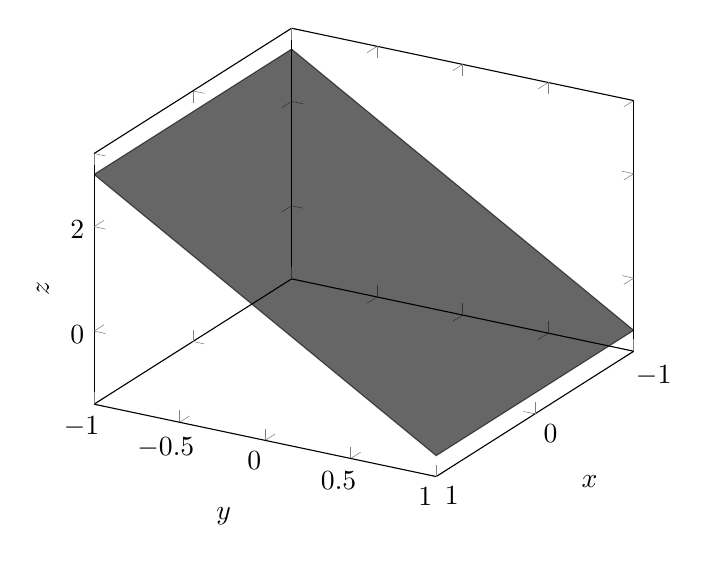
\begin{tikzpicture}
                \begin{axis}[xlabel=$x$,ylabel=$y$,zlabel=$z$,view={120}{30}]
                    \addplot3 [fill,opacity=0.6] coordinates {
                        (-1,-1,3)
                        (-1,1,-1)
                        (1,1,-1)
                        (1,-1,3)
                        (-1,-1,3)
                    };
                \end{axis}
            \end{tikzpicture}
        \end{center}
    }

    \item (5.3节例6)确定平面$x+2y+z-1=0$在三个坐标轴上的截距,并画出它在第一卦限内的图像。
    
    \sol{
        直接令$y=z=0$、$x=z=0$、$x=y=0$可知其在$x$、$y$、$z$轴上的截距为1、$\frac{1}{2}$、1,作出图像如下:
        \begin{center}
            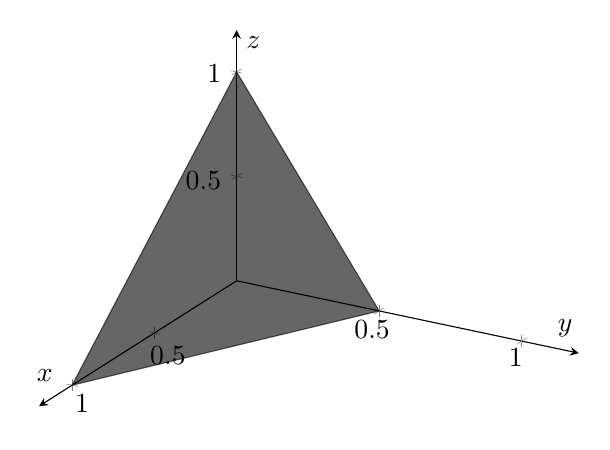
\begin{tikzpicture}
                \begin{axis}[axis lines=center,xlabel=$x$,ylabel=$y$,zlabel=$z$,view={120}{30},xmin=0,xmax=1.2,ymin=0,ymax=1.2,zmin=0,zmax=1.2]
                    \addplot3 [fill,opacity=0.6] coordinates {
                        (1,0,0)
                        (0,0.5,0)
                        (0,0,1)
                        (1,0,0)
                    };
                \end{axis}
            \end{tikzpicture}
        \end{center}
    }

    \item (5.3节例7)作出方程$3x-2y-z=0$表示的平面。
    
    \sol{
        由于它过原点,考虑它与$Oxy$平面($z=0$)的交线$3x-2y=0$、与$Ozx$平面($y=0$)的交线$3x-z=0$即可作出图像如下:
        \begin{center}
            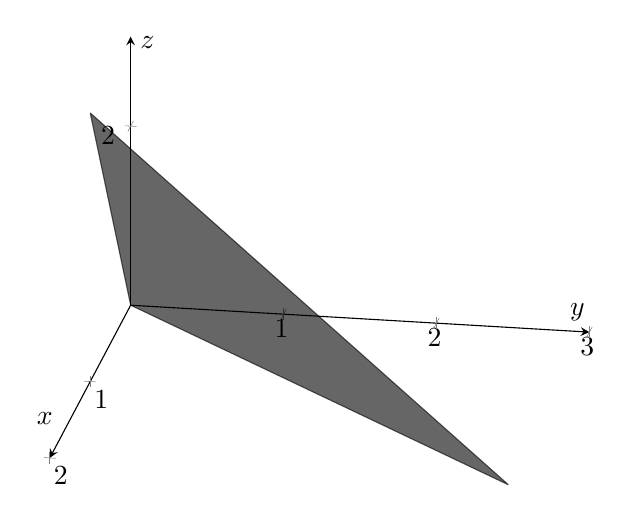
\begin{tikzpicture}
                \begin{axis}[axis lines=center,xlabel=$x$,ylabel=$y$,zlabel=$z$,view={100}{30}]
                    \addplot3 [fill,opacity=0.6] coordinates {
                        (0,0,0)
                        (2,3,0)
                        (1,0,3)
                        (0,0,0)
                    };
                \end{axis}
            \end{tikzpicture}
        \end{center}
    }

    \item (5.3节例8)确定常数$l$与$k$使得平面$x+ly+kz=1$与平面$x+y-z=8$垂直,且过点$(1,1,-\frac{2}{3})$。
    
    \sol{
        两平面垂直当且仅当它们的\textbf{法向量}垂直,因此列出方程
        $$\begin{cases}(1,l,k)\cdot(1,1,-1)=0\\1+l-\frac{2}{3}k=1\end{cases}$$
        解得$l=2$、$k=3$。
    }

    \item (5.3节例9)作出方程
    $$\begin{cases}x-3=0\\y-4=0\end{cases}$$
    表示的直线。

    \sol{
        由于其解为所有$(3,4,z),z\in\rb$,它表示一条平行$z$轴的直线,作出图像如下(实线部分为所求直线):
        \begin{center}
            \begin{tikzpicture}
                \begin{axis}[axis lines=center,xlabel=$x$,ylabel=$y$,zlabel=$z$,view={120}{30}]
                    \addplot3 [dashed] coordinates {
                        (3,4,3) (0,4,3) (0,4,0) (3,4,0) (3,4,3)
                    };
                    \addplot3 [dashed] coordinates {
                        (3,4,3) (3,0,3) (3,0,0) (3,4,0) (3,4,3)
                    };
                    \addplot3 [thick] coordinates {
                        (3,4,-0.5) (3,4,3.5)
                    };
                \end{axis}
            \end{tikzpicture}
        \end{center}
    }

    \item (5.3节例10)作出方程
    $$\begin{cases}x-1=0\\2y+z-1=0\end{cases}$$
    表示的直线。

    \sol{
        我们先作出$x=1$平面,再考虑平面$2y+z-1=0$与此平面的交线,即得到所求直线,作出图像如下(实线部分为所求直线):
        \begin{center}
            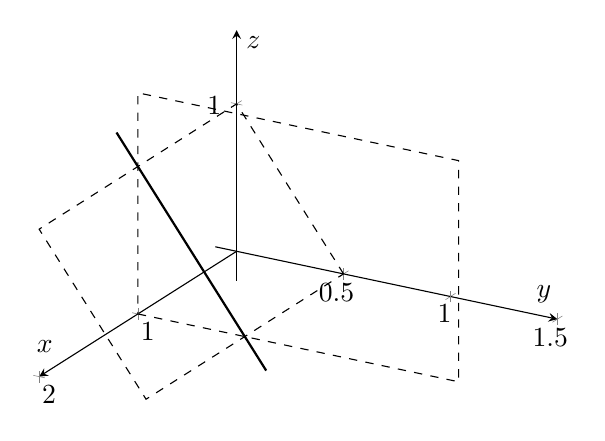
\begin{tikzpicture}
                \begin{axis}[axis lines=center,xlabel=$x$,ylabel=$y$,zlabel=$z$,view={120}{30}]
                    \addplot3 [dashed] coordinates {
                        (1,0,0) (1,1.5,0) (1,1.5,1.5) (1,0,1.5) (1,0,0)
                    };
                    \addplot3 [dashed] coordinates {
                        (0,0.5,0) (0,0,1) (2,0,1) (2,0.5,0) (0,0.5,0)
                    };
                    \addplot3 [thick] coordinates {
                        (1,-0.1,1.2) (1,0.6,-0.2)
                    };
                \end{axis}
            \end{tikzpicture}
        \end{center}
    }

    \item (5.3节例11)将直线的一般方程
    $$\begin{cases}x-y+z-1=0\\2x+y-3z=0\end{cases}$$
    化成标准方程。

    \sol{
        联立并利用线性代数知识可得到此方程组的两个解
        $$\bigg(0,-\frac{3}{2},-\frac{1}{2}\bigg),\quad\bigg(\frac{1}{3},-\frac{2}{3},0\bigg)$$
        从而作差可得此直线的一个方向向量$(\frac{1}{3},\frac{5}{6},\frac{1}{2})$,由乘非零倍数仍为方向向量可将其化为$(2,5,3)$,从而直线标准方程为
        $$\frac{x}{2}=\frac{y+\frac{3}{2}}{5}=\frac{z+\frac{1}{2}}{3}$$

        \note 直接求解两个点得到方向向量一般比计算叉乘\textbf{更快}。
    }

    \item (5.3节习题11改编)证明以下两条直线异面,并计算距离:
    $$\frac{x-1}{-1}=\frac{y}{2}=\frac{z+1}{1},\quad\frac{x+2}{0}=\frac{y-1}{1}=\frac{z-2}{-2}$$

    \sol{
        直接计算可发现两直线的方向向量$(-1,2,1)$与$(0,1,-2)$不成比例,因此两直线不平行。

        下面计算两直线的距离:设向量$(a,b,c)$与两条直线都垂直,可发现
        $$(a,b,c)\cdot(-1,2,1)=(a,b,c)\cdot(0,1,-2)=0$$
        利用线性代数知识可得一个非零解$(5,2,1)$。由几何关系可发现,两\textbf{不平行}的直线上各自任取一点,得到的向量在公垂线上的\textbf{投影}长度即为距离。

        利用内积的\textbf{几何意义}可知投影的长度为
        $$\bigg|\frac{((1,0,-1)-(-2,1,2))\cdot(5,2,1)}{|(5,2,1)|}\bigg|=\frac{10}{\sqrt{30}}=\frac{\sqrt{30}}{3}$$
        从而这就是两条直线的距离,由其非零两直线不可能相交,综合可知两直线异面。
    }

    \note 建议大家\textbf{记忆异面直线距离算法}。

    \item (5.4节结论)写出所有9种非线性的二次曲面的标准方程,并绘制草图。
    
    \note 除了上述9种外,还有6种三维空间中二次方程可能确定的点集形状:
    \begin{compactitem}
        \item 空集($x^2+y^2+z^2=-1$)
        \item 点($x^2+y^2+z^2=0$)
        \item 直线($x^2+y^2=0$)
        \item 平面($x^2=0$)
        \item 一对平行平面($x^2-a=0$,其中$a>0$)
        \item 一对相交平面($x^2-ay^2=0$,其中$a\in(0,1]$)
    \end{compactitem}
    本章中将进行更详细的讨论。

    \sol{
        所有9种非线性的二次曲面为椭球面、单叶双曲面、双叶双曲面、椭圆锥面、椭圆柱面、双曲柱面、抛物柱面、椭圆抛物面、双曲抛物面,下面写出方程并绘制草图(所有草图都可以通过给定$z$后计算截线形状进行绘制,除了双曲抛物面情况相对复杂以外,其他8种都是不难确定空间形状的):
        \begin{enumerate}[(1)]
            \item \textbf{椭球面},对应方程为
            $$\frac{x^2}{a^2}+\frac{y^2}{b^2}+\frac{z^2}{c^2}=1,\quad a,b,c>0$$
            作出示意图像如下:
            
            \begin{center}
                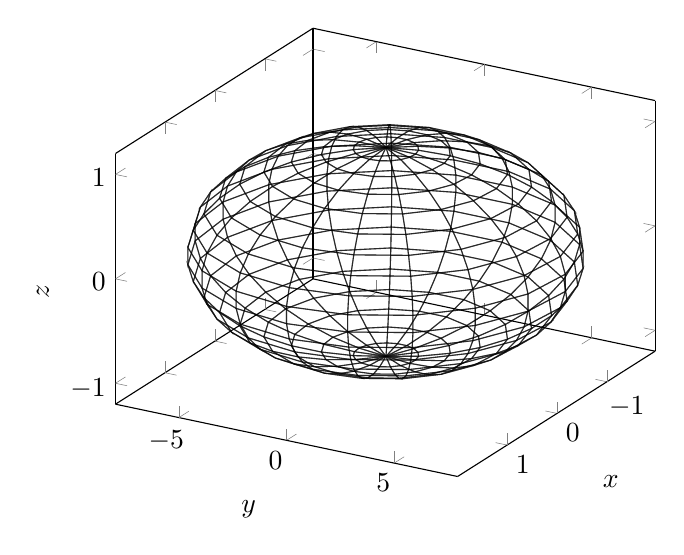
\begin{tikzpicture}
                    \begin{axis}[xlabel=$x$,ylabel=$y$,zlabel=$z$,view={120}{30}]
                        \addplot3 [mesh, z buffer=sort, samples=20, domain=0:pi, y domain=0:2*pi, opacity=0.6, color=black]
                            ({2 * sin(deg(x)) * cos(deg(y))},
                            {8 * sin(deg(x)) * sin(deg(y))},
                            {cos(deg(x))});
                    \end{axis}
                \end{tikzpicture}
            \end{center}

            \item \textbf{单叶双曲面},对应方程为
            $$\frac{x^2}{a^2}+\frac{y^2}{b^2}-\frac{z^2}{c^2}=1,\quad a,b,c>0$$
            作出示意图像如下:
            \begin{center}
                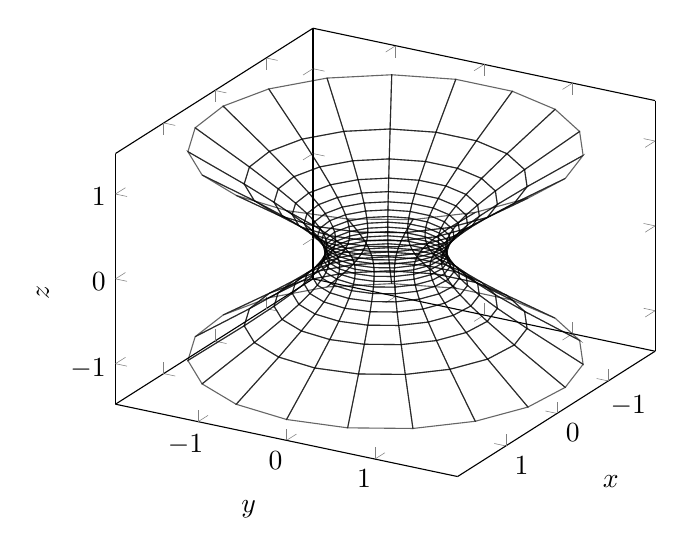
\begin{tikzpicture}
                    \begin{axis}[xlabel=$x$,ylabel=$y$,zlabel=$z$,view={120}{30}]
                        \addplot3 [mesh, z buffer=sort, samples=20, domain=-0.4*pi:0.4*pi, y domain=0:2*pi, opacity=0.6, color=black]
                            ({0.6 * sec(deg(x)) * cos(deg(y))},
                            {0.6 * sec(deg(x)) * sin(deg(y))},
                            {0.4 * tan(deg(x))});
                    \end{axis}
                \end{tikzpicture}
            \end{center}

            \item \textbf{双叶双曲面},对应方程为
            $$\frac{x^2}{a^2}+\frac{y^2}{b^2}-\frac{z^2}{c^2}=-1,\quad a,b,c>0$$
            作出示意图像如下:
            \begin{center}
                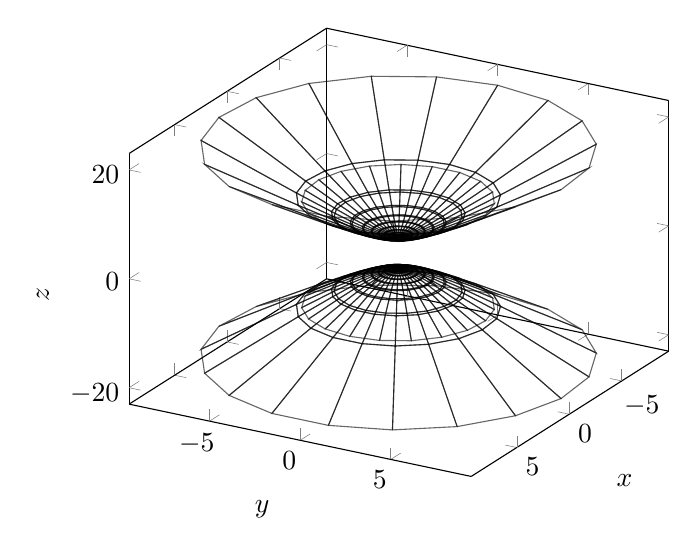
\begin{tikzpicture}
                    \begin{axis}[xlabel=$x$,ylabel=$y$,zlabel=$z$,view={120}{30}]
                        \addplot3 [mesh, z buffer=sort, samples=20, domain=0.55*pi:1.4*pi, y domain=0:2*pi, opacity=0.6, color=black]
                            ({1.5 * tan(deg(x)) * cos(deg(y))},
                            {1.5 * tan(deg(x)) * sin(deg(y))},
                            {3 * sec(deg(x))});
                        \addplot3 [mesh, z buffer=sort, samples=20, domain=0.55*pi:1.4*pi, y domain=0:2*pi, opacity=0.6, color=black]
                            ({1.5 * tan(deg(x)) * cos(deg(y))},
                            {1.5 * tan(deg(x)) * sin(deg(y))},
                            {-3 * sec(deg(x))});
                    \end{axis}
                \end{tikzpicture}
            \end{center}

            \item \textbf{椭圆锥面},对应方程为
            $$\frac{x^2}{a^2}+\frac{y^2}{b^2}-\frac{z^2}{c^2}=0,\quad a,b,c>0$$
            作出示意图像如下:
            \begin{center}
                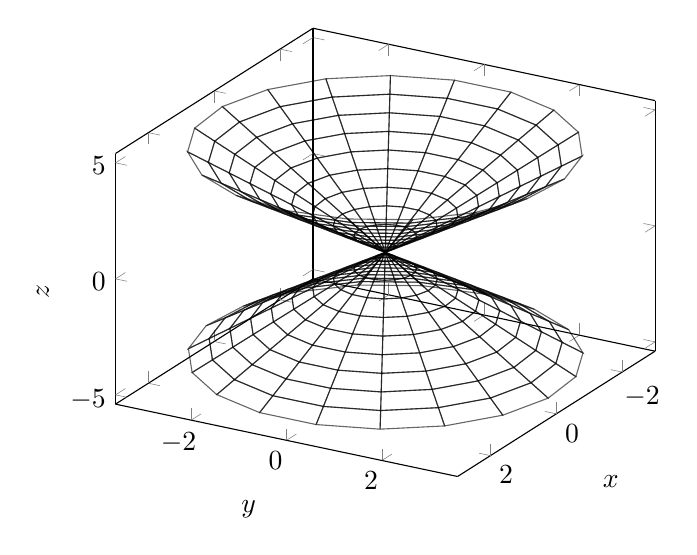
\begin{tikzpicture}
                    \begin{axis}[xlabel=$x$,ylabel=$y$,zlabel=$z$,view={120}{30}]
                        \addplot3 [mesh, z buffer=sort, samples=20, domain=-3:3, y domain=0:2*pi, opacity=0.6, color=black]
                            ({x * cos(deg(y))},
                            {1.2 * x * sin(deg(y))},
                            {1.5 * x});
                    \end{axis}
                \end{tikzpicture}
            \end{center}

            \item \textbf{椭圆柱面},对应方程为
            $$\frac{x^2}{a^2}+\frac{y^2}{b^2}=1,\quad a,b>0$$
            作出示意图像如下:
            \begin{center}
                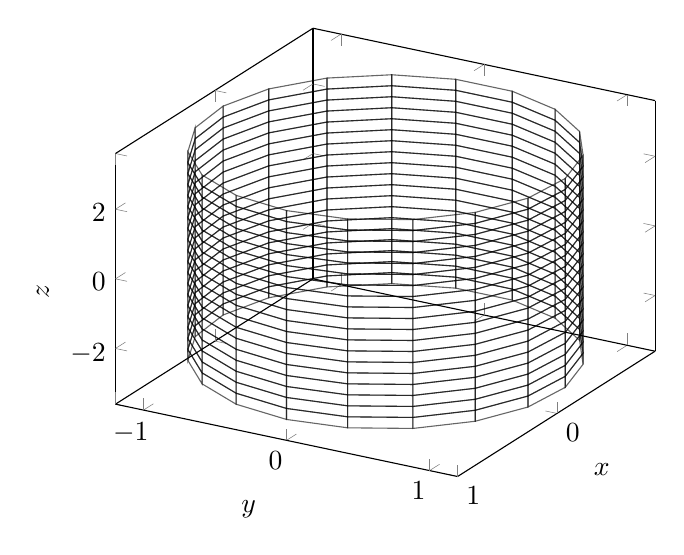
\begin{tikzpicture}
                    \begin{axis}[xlabel=$x$,ylabel=$y$,zlabel=$z$,view={120}{30}]
                        \addplot3 [mesh, z buffer=sort, samples=20, domain=-3:3, y domain=0:2*pi, opacity=0.6, color=black]
                            ({cos(deg(y))},
                            {1.2 * sin(deg(y))},
                            {x});
                    \end{axis}
                \end{tikzpicture}
            \end{center}

            \item \textbf{双曲柱面},对应方程为
            $$\frac{x^2}{a^2}-\frac{y^2}{b^2}=1,\quad a,b>0$$
            作出示意图像如下:
            \begin{center}
                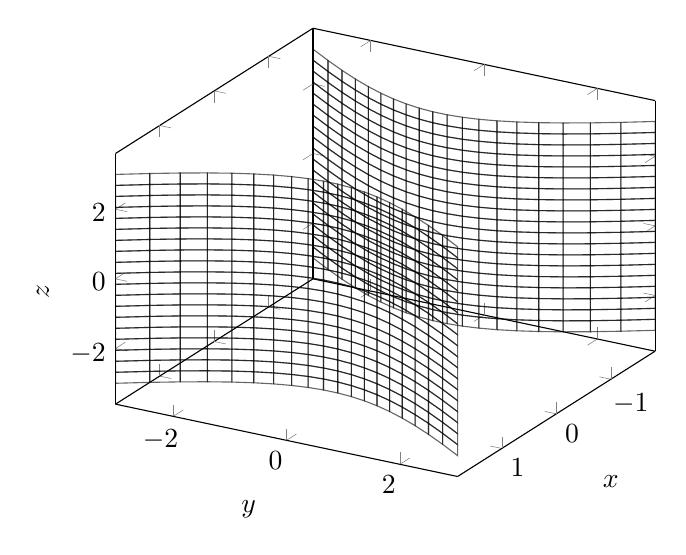
\begin{tikzpicture}
                    \begin{axis}[xlabel=$x$,ylabel=$y$,zlabel=$z$,view={120}{30}]
                        \addplot3 [mesh, z buffer=sort, samples=20, domain=-3:3, y domain=-1.2:1.2, opacity=0.6, color=black]
                            ({cosh(y)},
                            {2 * sinh(y)},
                            {x});
                        \addplot3 [mesh, z buffer=sort, samples=20, domain=-3:3, y domain=-1.2:1.2, opacity=0.6, color=black]
                            ({-cosh(y)},
                            {2 * sinh(y)},
                            {x});
                    \end{axis}
                \end{tikzpicture}
            \end{center}

            \item \textbf{抛物柱面},对应方程为
            $$\frac{x^2}{a^2}-y=0,\quad a>0$$
            作出示意图像如下:
            \begin{center}
                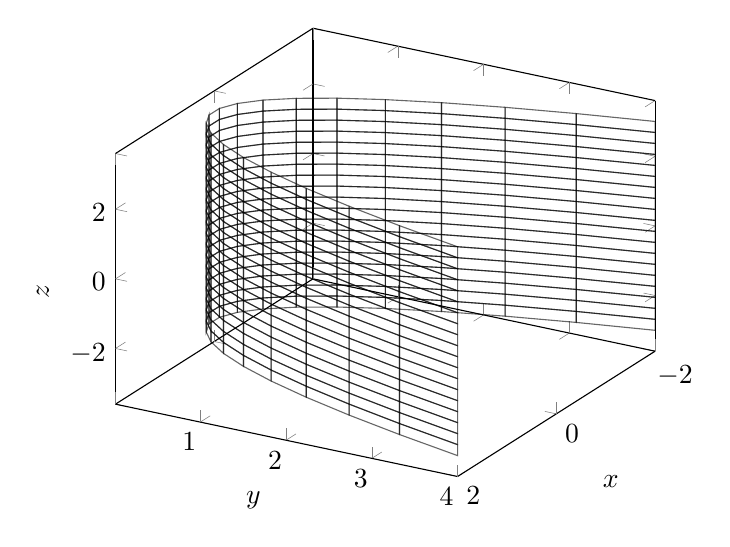
\begin{tikzpicture}
                    \begin{axis}[xlabel=$x$,ylabel=$y$,zlabel=$z$,view={120}{30}]
                        \addplot3 [mesh, z buffer=sort, samples=20, domain=-3:3, y domain=-2:2, opacity=0.6, color=black]
                            ({y},
                            {y^2},
                            {x});
                    \end{axis}
                \end{tikzpicture}
            \end{center}

            \item \textbf{椭圆抛物面},对应方程为
            $$\frac{x^2}{a^2}+\frac{y^2}{b^2}-z=0,\quad a,b>0$$
            作出示意图像如下:
            \begin{center}
                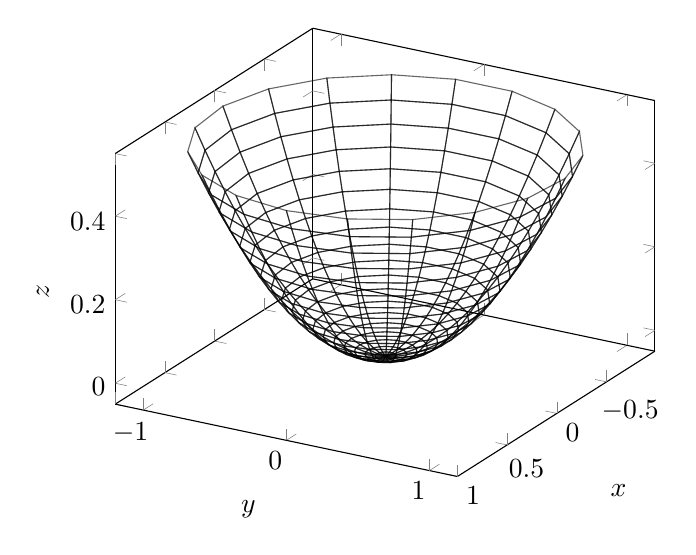
\begin{tikzpicture}
                    \begin{axis}[xlabel=$x$,ylabel=$y$,zlabel=$z$,view={120}{30}]
                        \addplot3 [mesh, z buffer=sort, samples=20, domain=0:1, y domain=0:2*pi, opacity=0.6, color=black]
                            ({x * cos(deg(y))},
                            {1.2 * x * sin(deg(y))},
                            {0.5 * x^2});
                    \end{axis}
                \end{tikzpicture}
            \end{center}

            \item \textbf{双曲抛物面},对应方程为
            $$\frac{x^2}{a^2}-\frac{y^2}{b^2}-z=0,\quad a>0$$
            作出示意图像如下:
            \begin{center}
                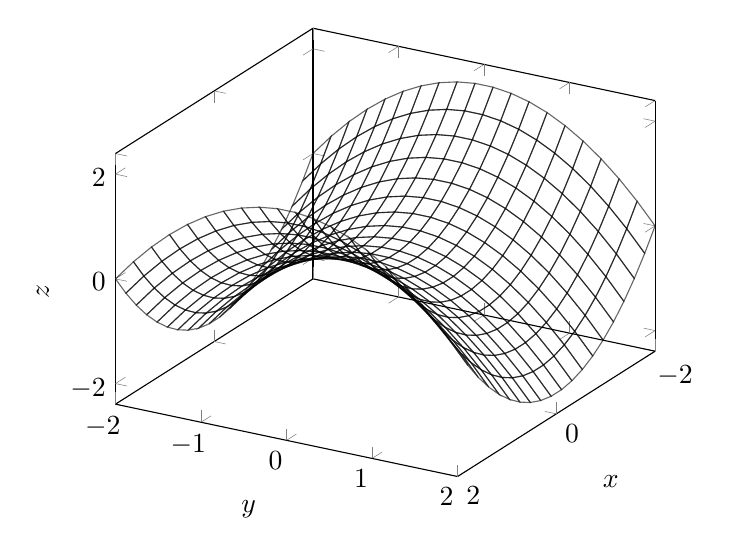
\begin{tikzpicture}
                    \begin{axis}[xlabel=$x$,ylabel=$y$,zlabel=$z$,view={120}{30}]
                        \addplot3 [mesh, z buffer=sort, samples=20, domain=-2:2, y domain=-2:2, opacity=0.6, color=black]
                            ({x},
                            {y},
                            {0.5 * (x^2 - y^2)});
                    \end{axis}
                \end{tikzpicture}
            \end{center}
        \end{enumerate}
    }

    \item (习题5.5.1)求下列曲线在指定点$P_0$处的切线与法平面方程:
    \begin{enumerate}
        \item[(2)] 曲线为$z=x^2$与$y=x$的交线,$P_0(2,2,4)$。
        
        \sol{
            此曲线可以直接写成\textbf{参数方程}
            $$(x(t),y(t),z(t))=(t,t,t^2),\quad t\in\rb$$
            于是
            $$(x'(t),y'(t),z'(t))=(1,1,2t)$$
            在$P_0$处$t=2$,从而可直接得到切方向$(1,1,4)$,切线方程为
            $$\frac{x-2}{1}=\frac{y-2}{1}=\frac{z-4}{4}$$
            而法平面为过这点且以切方向为法向量的平面,方程为
            $$(x-2)+(y-2)+4(z-4)=0$$
            即
            $$x+y+4z=20$$
        }
        

        \item[(3)] 曲线为$x^2+y^2=R^2$\ ($R>0$)与$z=x+y$的交线,$P_0(R,0,R)$。
        
        \sol{
            由它在$x^2+y^2=R^2$上,可设$x=R\cos\theta$、$y=R\sin\theta$,由此即得\textbf{参数方程}
            $$(x(\theta),y(\theta),z(\theta))=(R\cos\theta,R\sin\theta,R(\cos\theta+\sin\theta)),\quad\theta\in\rb$$

            于是
            $$(x'(\theta),y'(\theta),z'(\theta))=(-R\sin\theta,R\cos\theta,R(\cos\theta-\sin\theta))$$
            在$P_0$处可取$\theta=0$,从而可直接得到切方向$(0,R,R)$,切线方程为
            $$\frac{x-R}{0}=\frac{y-0}{R}=\frac{z-R}{R}$$
            而法平面为过这点且以切方向为法向量的平面,方程为
            $$0(x-R)+R(y-0)+R(z-R)=0$$
            即
            $$y+z=R$$

            \note 这里$\theta$增加$2\pi$后表示同一个点并不影响参数方程中$\theta$可以取任何实数。由于$x$、$y$、$z$对$\theta$的周期性,它们对$\theta$的导数也必然具有周期性,因此任取符合呀求的$\theta$不会影响切线计算结果。
        }
    \end{enumerate}

    \item (习题5.5.2)给定参数$R>0$、$b>0$,求螺旋线
    $$\begin{cases}x=R\cos t\\y=R\sin t\\z=bt\end{cases},\quad t\in[0,2\pi]$$
    在任何一点处切线的方向余弦,并证明该螺旋线任何一点的切线与$z$方向夹角为常数。
    
    \sol{
        对任何$t\in(0,2\pi)$,直接求导可知
        $$\bm{r}'(t)=(x'(t),y'(t),z'(t))=(-R\sin t,R\cos t,b)$$
        从而直接计算可知$|\bm{r}'(t)|=\sqrt{R^2+b^2}\ne0$,于是利用方向角定义有
        $$\cos\alpha=\frac{\bm{r}'(t)\cdot(1,0,0)}{|\bm{r}'(t)|}=-\frac{R}{\sqrt{R^2+b^2}}\sin t$$
        $$\cos\beta=\frac{\bm{r}'(t)\cdot(0,1,0)}{|\bm{r}'(t)|}=\frac{R}{\sqrt{R^2+b^2}}\cos t$$
        $$\cos\gamma=\frac{\bm{r}'(t)\cdot(0,0,1)}{|\bm{r}'(t)|}=\frac{b}{\sqrt{R^2+b^2}}$$
        由$\cos\gamma$不变即得与$z$方向夹角为常数。
    }
\end{enumerate}

\subsection{空间的几何}
在结束了一元微积分的研究后,从本章开始,我们将进入\textbf{多元微积分}的研究,也即研究$\rb^n$中的函数与映射相关的极限与微积分。不过,在给出这些的定义之前,我们需要了解$\rb^n$中的基本\textbf{几何与拓扑}结论。本节先介绍几何相关的结论,下节我们将说明何为拓扑、需要知道的拓扑结论有哪些。

本节中,我们所有的讨论几乎都将遵循如下的三步流程:
\begin{itemize}
    \item 先在\textbf{低维空间}(二维或三维)建立几何直观;
    \item 再把\textbf{低维空间}的几何直观在坐标系中用\textbf{代数}(也即中学所说的\textbf{解析几何}),作为\textbf{严谨定义};
    \item 将定义推广到\textbf{高维空间}中,研究一般的性质。
\end{itemize}
接下来我们将看到,如何通过这个流程将我们熟悉或不熟悉的种种几何概念在高维空间里进行代数化。

\subsubsection{直线与平面}
首先,我们需要从最简单的几何概念,\textbf{直线}与\textbf{平面}开始。我们知道,$\rb^2$或$\rb^3$的一个点可以用坐标$A(x_1,x_2)$或$A(x_1,x_2,x_3)$表示,它同样可以\textbf{等同}为一个向量$\overrightarrow{OA}$\ ($O$为原点),向量的坐标也为$(x_1,x_2)$或$(x_1,x_2,x_3)$。

在$\rb^n$\ (称为$n$维\textbf{欧氏空间})中,任何一个点或向量可以用$n$元组$(x_1,x_2,\dots,x_n)$表示,其每个分量都在$\rb$中。当我们写$\bm{x}\in\rb^n$时,指的即是$\bm{x}$是这样的一个$n$元组,用$x_i$表示$\bm{x}$的第$i$个分量。此外,$\rb^n$中的向量运算与$\rb^3$中相同,两个向量\textbf{相加}对应\textbf{各分量对应相加},一个向量\textbf{数乘}代表各分量都乘这个数。

\note 接下来的讨论过程可能用到向量加法、数乘的一些基本运算律,大家可以自行验证计算合理。

有了向量描述以后,我们即可以开始思考何为直线与平面。先从直线开始说起,我们默认讨论$\rb^3$中的直线与平面,$\rb^2$中的情况更加简单。

\

从直观来看,直线是一点向\textbf{一个方向}无限延伸的结果,也即,给定一点$\bm{\alpha}\in\rb^3$与一个方向$\bm{\beta}\in\rb^3$,我们需要从代数上给出\textbf{无限延伸}的定义。

在高中,我们知道将一个向量数乘就是几何上将它\textbf{延伸到指定倍数},而两个向量的加法则是将\textbf{第二个向量接到第一个的末尾},由此,$\bm{\alpha}+\bm{\beta}$即代表从$\bm{\alpha}$出发,延伸向量$\bm{\beta}$的结果,而如果要表达作任意长度的延伸,对应的点集即为
$$\{\bm{\alpha}+t\bm{\beta}\mid t\in\rb\}$$
这就表示$\rb^3$中所有从$\bm{\alpha}$向$\bm{\beta}$方向延伸的定义,当然,为了让\textbf{方向}有意义,我们需要让$\bm{\beta}\ne\bm{0}$。

综合以上,我们最终得到的直线的方程:给定点$\bm{\alpha}\in\rb^3$与方向$\bm{\beta}\in\rb^3$、$\bm{\beta}\ne\bm{0}$,直线对应的点集即
$$\{\bm{\alpha}+t\bm{\beta}\mid t\in\rb\}$$
或写为参数方程的形式,即直线上任一点$\bm{x}=(x,y,z)$满足
$$\begin{cases}x=\alpha_1+t\beta_1\\y=\alpha_2+t\beta_2\\z=\alpha_3+t\beta_3\end{cases},\quad t\in\rb$$
由此我们也可将$\bm{x}$看作$t$的函数,写为$\bm{x}(t)$。此参数方程称为直线的\textbf{标准方程}。

\note 我们也可以把方程\textbf{形式上}写作$\frac{x-\alpha_1}{\beta_1}=\frac{y-\alpha_2}{\beta_2}=\frac{z-\alpha_3}{\beta_3}$,若$\beta_i=0$代表着对应分母恒为0。由于此形式本质上并不方便,讲义上将\textbf{不使用此形式}。

当然,一个常见的使用情况是\textbf{给定两点}$\bm{\alpha}$、$\bm{\beta}$求直线方程,此时对应的方向即为$\bm{\beta}-\bm{\alpha}$,于是直线方程可以写为$\{\bm{\alpha}+t(\bm{\beta}-\bm{\alpha})\mid t\in\rb\}$。此外,虽然直线的方向是唯一的,从几何来说,\textbf{相差倍数}仍然代表同一方向,由此若直线$l$的方向是$\bm{d}$,所有$\lambda\bm{d}$\ ($\lambda\ne0$)仍然是直线的方向。

\

对于平面,它对应一点向\textbf{两个不同方向}任意延伸的结果,由此仿照之前,设点为$\bm{\alpha}$、方向为$\bm{\beta}$、$\bm{\gamma}$,可以将方程写为
$$\{\bm{\alpha}+t\bm{\beta}+s\bm{\gamma}\mid t,s\in\rb\}$$
不过,对于平面的一个困难在于,如何描述\textbf{不同方向}。在之前我们已经讨论过,方向乘倍数仍然是同一个方向,由此$\bm{\beta}$与$\bm{\gamma}$满足的关系为(最后一段即不存在非零的$\lambda$使得$\bm{\beta}$为$\lambda$倍$\bm{\gamma}$,这称为两向量\textbf{不相差非零倍数})
$$\bm{\beta}\ne\bm{0},\quad\bm{\gamma}\ne\bm{0},\quad\nexists\lambda\ne0,\quad\bm{\beta}=\lambda\bm{\gamma}$$
不过,此条件过于复杂,我们尝试给出一个更简单的描述。

\begin{framed}
\begin{exercise}
    证明$\rb^3$中的向量$\bm{y}$、$\bm{z}$满足
    $$\bm{y}\ne\bm{0},\quad\bm{z}\ne\bm{0},\quad\nexists\lambda\ne0,\quad\bm{y}=\lambda\bm{z}$$
    当且仅当关于$\lambda$与$\mu$的方程组$\lambda\bm{y}+\mu\bm{z}=0$解只有$\lambda=\mu=0$。
\end{exercise}
\sol{
    \begin{itemize}
        \item \textbf{上推下}
        
        若$\lambda\bm{y}+\mu\bm{z}=0$有$\lambda\ne0$的解,可发现
        $$\bm{y}=-\frac{\mu}{\lambda}\bm{z}$$
        若$\mu=0$则有$\bm{y}=0$,若$\mu\ne0$则$\bm{y}$是$\bm{z}$的非零倍数,也矛盾,从而不可能。

        由此可知解中必然$\lambda=0$,此时若$\mu\ne0$可知$\bm{z}=0$,矛盾,于是只能$\lambda=\mu=0$。

        \item \textbf{下推上}
    
        若$\bm{y}=0$,方程组有解$\lambda=1$、$\mu=0$,矛盾;若$\bm{z}=0$,方程组有解$\lambda=0$、$\mu=1$,矛盾。

        若存在非零的$t$使得$\bm{y}=t\bm{z}$,方程组有解$\lambda=1$、$\mu=-t$,矛盾。
    \end{itemize}

    \note 上述证明并没有用到$\rb^3$的条件,由此对$\rb^n$也成立。
}
\end{framed}

我们将上题中的描述称为$\bm{y}$与$\bm{z}$\textbf{线性无关},线性无关的定义可以推广到$\rb^n$中的任何$m$个向量,也即向量$\bm{y}_1,\dots,\bm{y}_m$线性无关当且仅当对$\lambda_1,\dots,\lambda_m$的方程组
$$\lambda_1\bm{y}_1+\dots+\lambda_m\bm{y}_m=0$$
只有零解。\textbf{线性代数}课程中将详细讨论。

\note 由此可见,直线定义中方向$\bm{\beta}\ne0$的要求事实上也可表述为$\bm{\beta}$线性无关。

综合以上,我们最终得到平面的方程:给定点$\bm{\alpha}\in\rb^3$与\textbf{线性无关}的向量$\bm{\beta},\bm{\gamma}\in\rb^3$,平面对应的点集即
$$\{\bm{\alpha}+t\bm{\beta}+s\bm{\gamma}\mid t,s\in\rb\}$$
或写为参数方程的形式,即平面上任一点$\bm{x}=(x,y,z)$满足
$$\begin{cases}x=\alpha_1+t\beta_1+s\gamma_1\\y=\alpha_2+t\beta_2+s\gamma_2\\z=\alpha_3+t\beta_3+s\gamma_3\end{cases},\quad t,s\in\rb$$

\note 从几何直观上,直线是一维的,而平面是二维的,因此直线只有一个\textbf{自由参数}$t$,而平面需要两个\textbf{自由参数}$t$、$s$。

\

最后,我们来聊聊平面的\textbf{一般方程}。考虑对$(x,y,z)$的方程
$$Ax+By+Cz+D=0$$
只要$A$、$B$、$C$不全为0\ (这事实上意味着系数矩阵的秩为1),利用线性代数知识可证明必然存在$\bm{\alpha}\in\rb^3$与线性无关的向量$\bm{\beta},\bm{\gamma}\in\rb^3$使得其解集为$\{\bm{\alpha}+t\bm{\beta}+s\bm{\gamma}\mid t,s\in\rb\}$,由此这是一个平面方程。反过来,也可以证明任何平面方程都可以以此表示。于是,这即称为三维空间中平面的一般方程。

\note 平面的一般方程与参数方程之间的转化几乎必须通过求解方程进行,没有简单方法。

利用平面的一般方程,我们也可以用两个\textbf{相交平面的方程}表示直线,也即直线方程可以写作
$$\begin{cases}A_1x+B_1y+C_1z+D_1=0\\A_2x+B_2x+C_2y+D_2=0\end{cases}$$
只要上下为相交的平面方程,这即代表一个直线方程,称为直线的\textbf{一般方程}。

\note 我们只需要通过线性代数知识得到上述方程组的两组解$(x_1,y_1,z_1)$、$(x_2,y_2,z_2)$,即可从此方程组得到直线的一个\textbf{标准方程}。

\subsubsection{平行与垂直}
有了直线与平面的方程后,我们即可以开始研究高中熟悉的\textbf{位置关系}结论。本部分我们默认讨论内容在$\rb^3$中,粗体字母表示三维向量。

首先是\textbf{平行}与\textbf{相交}相关,我们逐个进行讨论:
\begin{itemize}
    \item \textbf{两直线平行}
    
    对于两直线来说,平行也即代表延伸\textbf{方向相同},由此两直线
    $$\{\bm{x}+t\bm{y}\mid t\in\rb\},\quad\{\bm{\alpha}+t\bm{\beta}\mid t\in\rb\}$$
    平行当且仅当$\bm{y}$、$\bm{\beta}$代表同一方向,也即乘非零倍数可从一个得出另一个。

    \note 这里视重合为\textbf{平行的特殊情况}。

    \item \textbf{两直线相交}
    
    根据定义,相交也即代表联立两方程\textbf{有解},从而两直线
    $$\{\bm{x}+t\bm{y}\mid t\in\rb\},\quad\{\bm{\alpha}+t\bm{\beta}\mid t\in\rb\}$$
    相交当且仅当方程组
    $$\bm{x}+t\bm{y}=\bm{\alpha}+s\bm{\beta}$$
    有解$t$、$s$。这可以通过线性代数理论确定。
    
    \item \textbf{两直线异面}
    
    根据定义,两直线异面当且仅当不平行且不相交,从而根据前两部分即可确定。值得一提的是,在上方定义下,从几何角度可以发现,两直线\textbf{重合}事实上等价于\textbf{平行且相交}。

    \item \textbf{直线与平面平行-参数方程}
    
    我们此处考虑直线$\{\bm{x}+t\bm{y}\mid t\in\rb\}$与平面$\{\bm{\alpha}+t\bm{\beta}+s\bm{\gamma}\mid t,s\in\rb\}$,对平面一般方程的更多性质将在介绍内积后讨论。

    利用几何关系可发现,直线与平面平行事实上是在说,在平面的方向中可以\textbf{找到直线的方向}。根据定义,平面除了$\bm{\alpha}$部分以外,剩下的$t\bm{\beta}+s\bm{\gamma}$均表示可能的\textbf{延伸方向}(只要$t$、$s$不全为0),这实际上等价于
    $$\exists t,s\in\rb,\quad\bm{y}=t\bm{\beta}+s\bm{\gamma}$$
    线性代数上将这称为$\bm{y}$可以用$\bm{\beta}$与$\bm{\gamma}$\textbf{线性表出}。

    \note 这里并未要求$t$、$s$不全为0,因为若全为0则右侧为零向量,与$\bm{y}\ne\bm{0}$矛盾。

    \note 进一步地,若直线与平面平行且\textbf{相交},则说明直线属于平面。
    
    \item \textbf{两平面平行-参数方程}
    
    在直线与平面平行的基础上,我们可以发现,两平面平行当且仅当其中一个上的\textbf{任意一条直线}都与另一个平行。考虑平面
    $$\{\bm{x}+t\bm{y}+s\bm{z}\mid t,s\in\rb\},\quad\{\bm{\alpha}+t\bm{\beta}+s\bm{\gamma}\mid t,s\in\rb\}$$
    由刚才的分析可知这等价于
    $$\forall t_1,s_1\in\rb,\quad\exists t_2,s_2\in\rb,\quad t_1\bm{y}+s_1\bm{z}=t_2\bm{\beta}+s_2\bm{\gamma}$$

    \note 若$t_1=s_1=0$,一定存在解$t_2=s_2=0$,否则由线性无关定义可知$t_1\bm{y}+s_1\bm{z}\ne\bm{0}$,$t_2$、$s_2$也不会全为0。因此,我们还是无需在条件中特别指出不全为0。

    \note 进一步地,若两平面平行且\textbf{相交},则说明两平面重合。
\end{itemize}

\

不过,刻画完平行后,另一个常见的位置关系,也就是\textbf{垂直},会显得难以刻画。想要刻画垂直,我们必须有一个刻画向量\textbf{夹角}的手段。幸运的是,我们在高中已经学过了这样的手段:
\begin{framed}
\begin{exercise}
    对任何向量$\bm{x}\in\rb^3$,证明它的\textbf{长度}为
    $$|\bm{x}|=\sqrt{x_1^2+x_2^2+x_3^2}$$
    对任何非零向量$\bm{x},\bm{y}\in\rb^3$,证明它们的\textbf{夹角}为
    $$\left<\bm{x},\bm{y}\right>=\arccos\frac{\bm{x}\cdot\bm{y}}{|\bm{x}||\bm{y}|},\quad\bm{x}\cdot\bm{y}=x_1y_1+x_2y_2+x_3y_3$$

    \note 由此长度也可写为$|\bm{x}|=\sqrt{\bm{x}\cdot\bm{x}}$。
\end{exercise}
\sol{
    对任何$\bm{x}$,考虑它到$Oxy$平面的投影$P(x_1,x_2,0)$,投影点到原点的距离由\textbf{勾股定理}应为$\sqrt{x_1^2+x_2^2}$。连接$\bm{x}$与$P$,由此投影相当于将$z$分量变为了0,这条线段的长度应为$|x_3|$\ (这里不妨设$x_3\ne0$,否则已经得证),且与$OP$垂直,从而再由勾股定理知
    $$|\bm{x}|=\sqrt{(\sqrt{x_1^2+x_2^2})^2+|x_3|^2}=\sqrt{x_1^2+x_2^2+x_3^2}$$

    考虑$\bm{x}$、$\bm{y}$、$O$构成的三角形,利用上方讨论类似可知$\bm{x}$、$\bm{y}$连线的长度为$|\bm{x}-\bm{y}|$,由\textbf{余弦定理}即得
    $$\cos\left<\bm{x},\bm{y}\right>=\frac{|\bm{x}|^2+|\bm{y}|^2-|\bm{x}-\bm{y}|^2}{2|\bm{x}||\bm{y}|}$$
    展开即可发现
    $$\frac{|\bm{x}|^2+|\bm{y}|^2-|\bm{x}-\bm{y}|^2}{2}=\bm{x}\cdot\bm{y}$$
    又由夹角范围$[0,\pi]$,两侧同取$\arccos$得证。
}
\end{framed}
我们将$|\bm{x}|$称为向量$\bm{x}$的\textbf{模长},模长为1的向量称为\textbf{单位向量}。直接计算可以发现,对任何非零向量$\bm{x}$,$\frac{\bm{x}}{|\bm{x}|}$是与$\bm{x}$同方向的单位向量,称为$\bm{x}$的\textbf{单位化}。由此,我们可以进一步刻画垂直相关的位置关系,因为非零向量垂直当且仅当夹角为$\frac{\pi}{2}$,也就当且仅当\textbf{内积为0}:
\begin{itemize}
    \item \textbf{平面的法向量}
    
    利用内积的角度,我们可以解释平面的\textbf{一般方程}:从几何关系的角度,平面应当有且仅有一个垂直的方向,称为它的\textbf{法向},与此平行的非零向量称为平面的一个\textbf{法向量}。若平面上一点为$\bm{\beta}$,其法向为$\bm{n}=(A,B,C)$,由垂直的定义可知平面上的$\bm{\alpha}$满足
    $$\bm{n}\bot(\bm{\alpha}-\bm{\beta})$$
    也即平面方程可以写为
    $$\{\bm{\alpha}\in\rb^3\mid\bm{n}\cdot(\bm{\alpha}-\bm{\beta})=0\}$$
    设$\bm{\alpha}=(x,y,z)$,上述方程即可以写为
    $$n_1(x-\beta_1)+n_2(y-\beta_2)+n_3(z-\beta_3)=0$$
    这称为平面的\textbf{点法式}方程,可以发现将常数提出即为一般式方程。

    反过来,由于平面上任何两个点形成的向量都与法向量垂直,在一般式方程$Ax+By+Cz+D=0$中,$(A,B,C)$就是平面的法向量。
    
    \item \textbf{一般方程下的平行关系}
    
    考虑直线$\{\bm{\alpha}+t\bm{\beta}\mid t\in\rb\}$与平面$Ax+By+Cz+D=0$,利用垂直关系,直线与平面平行当且仅当直线与\textbf{法向量垂直},从而这等价于
    $$\bm{\beta}\cdot(A,B,C)=0$$

    \note 事实上,由于形式相对直接,对直线我们\textbf{常用参数方程},对平面则\textbf{常用一般方程},一般建议大家如此化简表示。

    对于两平面$A_1x+B_1y+C_1z+D_1=0$、$A_2x+B_2y+C_2z+D_2=0$,它们平行则当且仅当\textbf{法向相同},也即$(A_1,B_1,C_1)$与$(A_2,B_2,C_2)$相差非零倍数。

    \item \textbf{两直线垂直}
    
    考虑直线
    $$\{\bm{x}+t\bm{y}\mid t\in\rb\},\quad\{\bm{\alpha}+t\bm{\beta}\mid t\in\rb\}$$
    由于两直线垂直也即代表\textbf{方向相互垂直},这等价于
    $$\bm{y}\cdot\bm{\beta}=0$$

    \item \textbf{直线与平面垂直}
    
    考虑直线$\{\bm{\alpha}+t\bm{\beta}\mid t\in\rb\}$与平面$Ax+By+Cz+D=0$。

    由于直线与平面垂直即意味着直线的方向与平面的\textbf{法向量}平行,这当且仅当$\bm{\beta}$与$(A,B,C)$相差非零倍数。

    \item \textbf{两平面垂直}
    
    考虑两平面$A_1x+B_1y+C_1z+D_1=0$、$A_2x+B_2y+C_2z+D_2=0$。从几何关系可知,两平面垂直\textbf{当且仅当}法向量相互垂直,由此这当且仅当
    $$(A_1,B_1,C_1)\cdot(A_2,B_2,C_2)=0$$

\end{itemize}

\

接下来,我们引入三个概念,\textbf{投影长度}、\textbf{方向余弦}与\textbf{外积}。

在三维空间中,我们记$x$、$y$、$z$方向的单位向量为
$$\bm{i}=(1,0,0),\quad\bm{j}=(0,1,0),\quad\bm{k}=(0,0,1)$$
可以发现,$\bm{\alpha}\cdot\bm{i}=\alpha_1$,这即是$\bm{\alpha}$在$x$方向的\textbf{有向投影长度}(沿$\bm{i}$方向为正,否则为负)。一般地,$\bm{\alpha}$与任何单位向量的内积代表它在对应方向的有向投影长度。

\note 利用投影长度可以方便地得到一些\textbf{距离}相关的公式,见本讲义13.1第7题、第17题等。

若$\bm{\alpha}$非零,将这个值除以$\frac{1}{|\bm{\alpha}|}$,得到的$\frac{\bm{\alpha}\cdot\bm{i}}{|\bm{\alpha}|}$称为它在$x$方向的\textbf{方向余弦},也即$\bm{\alpha}$与$x$轴夹角的余弦值。由性质可发现它与$\bm{\alpha}$的单位化的$x$分量相同,由此$x$、$y$、$z$三个方向的\textbf{方向余弦平方和为1}。

对于任何两个向量$\bm{x},\bm{y}\in\rb^3$,我们定义它们的\textbf{外积}(或\textbf{叉乘})为向量
$$\bm{x}\times\bm{y}=(x_2y_3-x_3y_2,x_3y_1-x_1y_3,x_1y_2-x_2y_1)$$
可以直线验证它的如下性质:
\begin{itemize}
    \item $\bm{x}\times\bm{y}$与$\bm{x}$、$\bm{y}$均垂直;
    \item $\bm{x}\times\bm{y}=\bm{0}$当且仅当$\bm{x}$、$\bm{y}$线性相关(从而对非零向量,叉乘为0说明\textbf{相差非零倍数},可用于\textbf{判定平行});
    \item $\bm{x}\times\bm{y}=-\bm{y}\times\bm{x}$;
    \item $\lambda(\bm{x}\times\bm{y})=(\lambda\bm{x})\times\bm{y}=\bm{x}\times(\lambda\bm{y})$;
    \item 外积\textbf{不具有结合律};
    \item 外积对加法有\textbf{分配律},也即
    $$\bm{x}\times(\bm{y}+\bm{z})=\bm{x}\times\bm{y}+\bm{x}\times\bm{z}$$
    $$(\bm{x}+\bm{y})\times\bm{z}=\bm{x}\times\bm{z}+\bm{y}\times\bm{z}$$
\end{itemize}

我们最后证明一个外积的常用性质:
\begin{exercise}
\begin{framed}
    对非零向量$\bm{x}$、$\bm{y}$,设它们夹角为$\theta$,则
    $$|\bm{x}\times\bm{y}|=|\bm{x}||\bm{y}|\sin\theta$$
    也即点$\bm{x}$、$\bm{y}$与原点构成的\textbf{三角形面积两倍}。
\end{framed}
\sol{
    由夹角范围在$[0,\pi]$,必然有$\sin\theta=\sqrt{1-\cos^2\theta}$,由此右侧即
    $$|\bm{x}||\bm{y}|\sqrt{1-\frac{(\bm{x}\cdot\bm{y})^2}{|\bm{x}|^2|\bm{y}|^2}}$$
    化简即
    $$\sqrt{|\bm{x}|^2|\bm{y}|^2-(\bm{x}\cdot\bm{y})^2}$$
    而利用定义可知左侧为
    $$\sqrt{(x_2y_3-x_3y_2)^2+(x_3y_1-x_1y_3)^2+(x_1y_2-x_2y_1)^2}$$
    直接展开后对比根号中的部分可知左右相等。
}
\end{exercise}

\subsubsection{高维情况}
\note 本部分内容\textbf{与考试无关},可以作为线性代数课程的一些直观应用,我们将\textbf{直接使用一些线性代数术语与结论}。

在一般的\textbf{欧氏空间}$\rb^n$中,我们无法再向$\rb^3$一样产生几何直观,因此必须进行\textbf{纯代数化}的定义。首先,对$\bm{x},\bm{y}\in\rb^n$,$\bm{x}$的\textbf{模长}可以定义为
$$|\bm{x}|=\sqrt{x_1^2+\dots+x_n^2}$$
两向量\textbf{内积}可以定义为
$$\bm{x}\cdot\bm{y}=x_1y_1+\dots+x_ny_n$$
\textbf{夹角}则定义为(注意多维时尖括号一般不代表夹角,而代表\textbf{生成},见之后的定义)
$$\arccos\frac{\bm{x}\cdot\bm{y}}{|\bm{x}||\bm{y}|}$$
于是非零向量\textbf{垂直}(或称为\textbf{正交})仍然等价于内积为0。

\note 夹角的结论仍然可以通过考虑两向量构成的三角形后由余弦定理证明。

\

可以发现,之前对于直线、平面\textbf{方向}的讨论仍然可以沿用,也即直线仍然可以写为
$$\{\bm{x}+t\bm{y}\mid t\in\rb\},\quad\bm{x},\bm{y}\in\rb^n$$
且要求$\bm{y}\ne\bm{0}$。

平面仍然可以写为
$$\{\bm{x}+t\bm{y}+s\bm{z}\mid t\in\rb\},\quad\bm{x},\bm{y},\bm{z}\in\rb^n$$
且要求$\bm{y}$、$\bm{z}$\textbf{线性无关}。

以此类推,我们似乎可以继续往后增加\textbf{独立的方向},直到方向个数达到$n-1$:利用线性代数知识可以证明,$n$维空间中若走向$n$个独立的方向,一定会到达全空间。

由此,我们可以给出如下的\textbf{推广}定义:给定$\bm{x}\in\rb^n$与\textbf{线性无关}的方向向量$\bm{\alpha}_1,\dots,\bm{\alpha}_k\in\rb^n$,称集合
$$\{\bm{x}+\lambda_1\bm{\alpha}_1+\dots+\lambda_k\bm{\alpha}_k\mid \lambda_1,\dots,\lambda_k\in\rb\}$$
为一个$k$维的\textbf{线性流形}(或称为\textbf{超平面}),这里$1\le k\le n-1$。在此定义下,无论在几维空间中,$k=1$的情况即对应\textbf{直线},$k=2$的情况即对应\textbf{平面}。

\note 流形这个词我们之后还会介绍,它的含义类似于曲面。而这里的``线性''即是指向量的\textbf{线性组合}(也即数乘后相加)。

我们用记号$\left<\bm{\alpha}_1,\dots,\bm{\alpha}_k\right>$表示集合
$$\{\lambda_1\bm{\alpha}_1+\dots+\lambda_k\bm{\alpha}_k\mid \lambda_1,\dots,\lambda_k\in\rb\}$$
也即所有能被$\bm{\alpha}_1,\dots,\bm{\alpha}_k$\textbf{线性表出}的向量。可以发现,此集合中的所有\textbf{非零向量}都是上述线性流形的延伸方向,因此称为此线性流形的\textbf{方向集合}。我们之后将上方的线性流形记作
$$\bm{x}+\left<\bm{\alpha}_1,\dots,\bm{\alpha}_k\right>$$
并将$k$称为它的\textbf{维度}。

\

与上一部分类似,我们可以讨论一般的\textbf{平行}与\textbf{垂直}:
\begin{itemize}
    \item \textbf{一般的平行定义}
    
    考虑两个线性流形
    $$\bm{x}+\left<\bm{\alpha}_1,\dots,\bm{\alpha}_k\right>$$
    $$\bm{y}+\left<\bm{\beta}_1,\dots,\bm{\beta}_s\right>$$
    若$k=s$,按我们之前对平面与直线的讨论可发现平行\textbf{当且仅当对应的方向集合相同},也即
    $$\left<\bm{\alpha}_1,\dots,\bm{\alpha}_k\right>=\left<\bm{\beta}_1,\dots,\bm{\beta}_s\right>$$
    若某个的维度更低,平行事实上指的是维度低的方向集合在维度高的方向集合当中,也即若$k<s$,平行指
    $$\left<\bm{\alpha}_1,\dots,\bm{\alpha}_k\right>\subset\left<\bm{\beta}_1,\dots,\bm{\beta}_s\right>$$
    若$k>s$同理定义。

    \item \textbf{一般的相交情况}
    
    利用线性代数理论,我们可以给出如下结论:一个$k$维的线性流形与一个$s$维的线性流形,若$k+s<n$则\textbf{一般不相交}(类比$\rb^3$中的两条直线),若$k+s\ge n$则交\textbf{一般}为一个$k+s-n$维的线性流形(0维线性流形即\textbf{一个点},可以考虑$\rb^3$中的一直线一平面与两平面)。

    \note 何为一般呢?从线性代数的角度来说,若它们分别为
    $$\bm{x}+\left<\bm{\alpha}_1,\dots,\bm{\alpha}_k\right>$$
    $$\bm{y}+\left<\bm{\beta}_1,\dots,\bm{\beta}_s\right>$$
    ``一般''事实上在$k+s<n$时指矩阵$(\bm{\alpha}_1,\dots,\bm{\alpha}_k,\bm{\beta}_1,\dots,\bm{\beta}_s,\bm{x}-\bm{y})$\textbf{列满秩秩};$k+s\ge n$时指矩阵$(\bm{\alpha}_1,\dots,\bm{\alpha}_k,\bm{\beta}_1,\dots,\bm{\beta}_s)$\textbf{行满秩}。
    
    \item \textbf{法向定义}
    
    类比直线与平面,对线性流形
    $$\bm{x}+\left<\bm{\alpha}_1,\dots,\bm{\alpha}_k\right>$$
    若一个非零向量$\bm{l}$满足
    $$\forall i=1,\dots,k,\quad\bm{l}\cdot\bm{\alpha}_i=0$$
    则称$\bm{l}$为此线性流形的一个\textbf{法向量}。

    利用线性代数中的\textbf{正交补}理论可以证明,一定存在\textbf{线性无关}的$\bm{l}_1,\dots,\bm{l}_{n-k}$使得此线性流形的\textbf{全部法向量}添加0后为
    $$\left<\bm{l}_1,\dots,\bm{l}_{n-k}\right>$$
    在$\rb^3$中,这也就代表直线有两个独立法向,而平面只有唯一的法向方向。
    
    \item \textbf{$n-1$维超平面}
    
    在$\rb^n$中,根据刚才的讨论,\textbf{仅有一个法向方向}的线性流形必然为$n-1$维。与平面类似,如果给定$n-1$维线性流形中的一个点$\bm{\beta}\in\rb^n$与\textbf{非零}法向量$\bm{\tau}\in\rb^n$,其上的所有点一定可以写为
    $$\{\bm{x}\in\rb^n\mid\bm{\tau}\cdot(\bm{x}-\bm{\beta})=0\}$$
    此即可以改写为
    $$\tau_1x_1+\dots+\tau_nx_n+(\tau_1\beta_1+\dots+\tau_n\beta_n)=0$$
    由此,类似\textbf{平面一般方程}形式的方程在$\rb^n$中表示一个$n-1$维的\textbf{超平面}。

    \item \textbf{一般的垂直定义}
    
    最后,我们尝试研究两个线性流形
    $$\bm{x}+\left<\bm{\alpha}_1,\dots,\bm{\alpha}_k\right>$$
    $$\bm{y}+\left<\bm{\beta}_1,\dots,\bm{\beta}_s\right>$$
    何时是\textbf{垂直}的。此问题事实上定义起来相对困难:对于一直线一平面或两平面来说,垂直只需要平面的法向包含在另一个的方向中,但对两直线垂直,又并不要求一个直线的全部法向包含在另一条直线的方向里。

    我们这里直接给出结论,大家可以尝试从\textbf{几何角度}进行理解:设集合
    $$V_1=\left<\bm{\alpha}_1,\dots,\bm{\alpha}_k\right>,\quad V_2=\left<\bm{\beta}_1,\dots,\bm{\beta}_s\right>$$
    并记
    $$W_1=\{\bm{w}\in V_1\mid\forall\bm{z}\in V_1\cap V_2,\quad\bm{w}\cdot\bm{z}=0\}$$
    $$W_2=\{\bm{w}\in V_2\mid\forall\bm{z}\in V_1\cap V_2,\quad\bm{w}\cdot\bm{z}=0\}$$
    则两线性流形垂直\textbf{当且仅当}$W_1$、$W_2$维度都高于0,且
    $$\forall\bm{w}_1\in W_1,\quad\forall\bm{w}_2\in W_2,\quad \bm{w}_1\cdot\bm{w}_2=0$$

    \note 这里$W_1$代表$V_1$中所有与$V_1\cap V_2$垂直的部分,$W_2$代表$V_2$中所有与$V_1\cap V_2$垂直的部分,此定义即代表,两线性流形垂直当且仅当$W_1$与$W_2$中的任何向量相互垂直。大家可以尝试从两平面相交的情况进行理解。
\end{itemize}

除此以外,$\rb^n$中的投影与方向余弦仍然可以类似定义,这样即可将距离等概念也推广到$\rb^n$中。不过,\textbf{有意义的叉乘仅能在$\rb^3$或$\rb^7$中定义},在其他维度的空间中不再具有性质一致的结构。对此的本质讨论涉及很深的数学,此处不再展开。

\subsubsection{曲线与曲面}
在介绍完$\rb^3$与$\rb^n$中的直线、平面的性质后,我们现在即需要定义\textbf{曲线}和\textbf{曲面}。我们仍然只讨论$\rb^3$中的情况,下方的$\bm{x}$均指$(x,y,z)$。

首先,为了定义曲线,一个自然的想法是从\textbf{直线}的参数方程形式
$$\begin{cases}x=\alpha_1+t\beta_1\\y=\alpha_2+t\beta_2\\z=\alpha_3+t\beta_3\end{cases},\quad t\in\rb$$
出发(这里要求$\bm{\beta}\ne\bm{0}$)。可以想到,既然当$x$、$y$、$z$都是$t$的一次函数时代表直线,如果是其他形式的函数,就能代表曲线了。

由此,我们考虑方程$\bm{x}=\bm{r}(t)$,即
$$\begin{cases}x=r_1(t)\\y=r_2(t)\\z=r_3(t)\end{cases},\quad t\in\rb$$
从几何直观的角度,我们至少希望$r_1$、$r_2$、$r_3$都是$t$的\textbf{连续}函数,否则曲线将失去意义——此时即称上述表达式为一条\textbf{连续曲线}。如无特殊说明,我们所说的曲线都默认指连续曲线。

除此之外,类比\textbf{线段}的定义,若上方的$t$范围不是$\rb$,而是某个\textbf{闭区间}$[a,b]$,$r_1$、$r_2$、$r_3$都是$[a,b]$上的连续函数,我们就称对应的方程为一个\textbf{曲线段},且它的起点为$\bm{r}(a)$、终点为$\bm{r}(b)$,可以称为\textbf{连接}$\bm{r}(a)$、$\bm{r}(b)$的曲线段。

在学习完求导后,我们自然希望通过导数来研究曲线的切线。由此,若$r_1$、$r_2$、$r_3$均存在导数,我们就称$\bm{x}=\bm{r}(t)$是一条\textbf{可微曲线},并记
$$\bm{r}'(t)=(r_1'(t),r_2'(t),r_3'(t))$$
对于可微曲线,利用导函数的\textbf{几何意义}可以想到,当$t=t_0$处产生微小变化$\Delta t$时,$\bm{r}(t)$的变化应当接近$(\Delta t)\bm{r}'(t_0)$,由此$\bm{r}'(t)$应当为其切线的方向,又切线过点$\bm{r}(t_0)$,即说明它在$t=t_0$处的切线方程应当为
$$\bm{x}=\bm{r}(t_0)+t\bm{r}'(t_0),\quad t\in\rb$$
但是,这里存在一种特殊情况:若$\bm{r}'(t_0)=\bm{0}$,上述方程只能得到一个点,\textbf{无法得到切线}。由此,我们将$\bm{r}'(t_0)\ne\bm{0}$的$t_0$称为可微曲线$\bm{x}=\bm{r}(t)$的\textbf{正则点},即意味着在这点处可以正常计算切线与法线。

\note 上述连续曲线、曲线段、可微曲线、切线、正则点的定义都可以\textbf{直接推广到$\rb^n$中}。

\

接下来考虑曲面。在$\rb^3$中,曲面有两种方程形式,一种是含两个参数的方程
$$\begin{cases}x=\alpha_1+t\beta_1+s\gamma_1\\y=\alpha_2+t\beta_2+s\gamma_2\\z=\alpha_3+t\beta_3+s\gamma_3\end{cases},\quad t,s\in\rb$$
另一种则是\textbf{一般方程}$Ax+By+Cz+D=0$。

对第一种方程,我们可以完全类似曲线将曲面方程定义为
$$\begin{cases}x=r_1(t,s)\\y=r_2(t,s)\\z=r_3(t,s)\end{cases},\quad t,s\in\rb$$
不过,这里的\textbf{连续性}、\textbf{可微性}等内容需要学完多元函数微分学以后才能严谨定义,此处先给出一些与曲线类似的定义,大家可以在学完下一章后\textbf{回头}阅读:
\begin{itemize}
    \item 若$r_1$、$r_2$、$r_3$都是$\rb^2$上的连续函数,称此方程对应一个\textbf{连续曲面}。如无特殊说明,我们所说的曲面均指连续曲面。
    \item 若$r_1$、$r_2$、$r_3$的实际定义域是$\rb^2$中的某区域,称对应的方程为一个\textbf{曲面片}。
    \item 若$r_1$、$r_2$、$r_3$都是$\rb^2$上处处可微的函数,则称方程对应一个\textbf{可微曲面}。
    \item 对可微曲面,记($i=1,2$)
    $$\partial_i\bm{r}(t,s)=(\partial_ir_1(t,s),\partial_ir_2(t,s),\partial_ir_3(t,s))$$
    记$\bm{n}=\partial_1\bm{r}(t_0,s_0)\times\partial_2\bm{r}(t_0,s_0)$,它非零的点称为曲面的\textbf{正则点},此时$\bm{n}$为曲面在$(t_0,s_0)$处的\textbf{法向量}。
\end{itemize}

对第二种方程,有结论:通常来说$F(x,y,z)=0$可以表示一个曲面。不过,它能确定曲面的条件事实上相对复杂,我们将在介绍\textbf{隐函数定理}时进一步讨论。

\

最后,所谓的\textbf{二次曲面}是指由关于$x$、$y$、$z$的二次方程
$$0=\Gamma(x,y,z)=Ax^2+By^2+Cz^2+Dyz+Exz+Fxy+Gx+Hy+Iz+J$$
确定的曲面,且要求$A$、$B$、$C$、$D$、$E$、$F$不全为0。它事实上是平面上的二次曲面在$\rb^3$中的\textbf{推广},就像二次曲线可以分为抛物线、椭圆、双曲线等,对于二次曲面的一个关键研究也是它的\textbf{分类}。具体来说,这里的分类标准是,如果两个二次曲线可以在平移、旋转后\textbf{重合},我们就认为它们相同。我们将用非常简短的篇幅对二次曲面分类的过程与结论进行介绍,大家\textbf{了解即可}。

利用\textbf{线性代数知识}可以证明,一定存在一个旋转使得$\Gamma(x,y,z)$在旋转后的方程变为
$$0=\Gamma_0(x,y,z)=A_0x^2+B_0y^2+C_0z^2+G_0x+H_0y+I_0z+J_0$$
且$A_0^2+B_0^2+C_0^2\ne0$。更进一步地,若$A_0\ne0$,我们就可以作平移$x\to x-\frac{G_0}{2A_0}$将一次项平移为0,由此类似讨论$B_0$、$C_0$法线,通过平移可以使得\textbf{二次项与一次项不共存}。这样,我们就可以初步将二次曲面分为(这里$A_0$、$B_0$、$C_0$均非零):
\begin{itemize}
    \item $A_0x^2+B_0y^2+C_0z^2+J_0=0$;
    \item $A_0x^2+B_0y^2+I_0z+J_0=0$;
    \item $A_0x^2+H_0y+I_0z+J_0=0$。
\end{itemize}
我们已经利用了$x$、$y$、$z$的对称性,也即通过\textbf{适当旋转}可以任意交换$x$、$y$、$z$,从而若只有一个二次项可不妨设$x$是二次项,有两个可不妨设为$x$与$y$。

进一步观察可发现,对于$A_0x^2+H_0y+I_0z+J_0=0$,通过绕$x$轴的旋转即能使得$H_0y+I_0z\to\sqrt{H_0^2+I_0^2}z$,从而最终需要讨论以下三类的细分:
\begin{itemize}
    \item $A_0x^2+B_0y^2+C_0z^2+J_0=0$
    
    利用对称性与方程可整体取负号,我们可不妨设$J_0\le0$,讨论$A_0$、$B_0$、$C_0$为正的数目,分为六类:
    \begin{enumerate}
        \item $J_0=0$,$A_0$、$B_0$、$C_0$均正或均负,对应\textbf{一点};
        \item $J_0=0$,$A_0$、$B_0$、$C_0$两正一负或两负一正,对应\textbf{椭圆锥面};
        \item $J_0<0$、$A_0$、$B_0$、$C_0$均正,对应\textbf{椭球面};
        \item $J_0<0$、$A_0$、$B_0$、$C_0$两正一负,对应\textbf{单叶双曲面};
        \item $J_0<0$、$A_0$、$B_0$、$C_0$两负一正,对应\textbf{双叶双曲面};
        \item $J_0<0$、$A_0$、$B_0$、$C_0$均负,对应\textbf{空集}。
    \end{enumerate}

    \item $A_0x^2+B_0y^2+I_0z+J_0=0$
    
    可以发现,若$I_0\ne0$,作平移可使$J_0=0$,从而只需讨论$I_0$或$J_0$至少有一个为0的情况(由方程可整体取负号可不妨设另一个非正):
    \begin{enumerate}
        \item $I_0<0$、$J_0=0$,$A_0$、$B_0$均正或均负,对应\textbf{椭圆抛物面};
        \item $I_0<0$、$J_0=0$,$A_0$、$B_0$一正一负,对应\textbf{双曲抛物面};
        \item $I_0=0$、$J_0<0$,$A_0$、$B_0$均正,对应\textbf{椭圆柱面};
        \item $I_0=0$、$J_0<0$,$A_0$、$B_0$一正一负,对应\textbf{双曲柱面};
        \item $I_0=0$、$J_0<0$,$A_0$、$B_0$均负,对应\textbf{空集};
        \item $I_0=0$、$J_0=0$,$A_0$、$B_0$均正或均负,对应\textbf{直线};
        \item $I_0=0$、$J_0=0$,$A_0$、$B_0$一正一负,对应\textbf{一对相交平面}。
    \end{enumerate}

    \item $A_0x^2+I_0z+J_0=0$
    
    与上一类相同,只需讨论$I_0$或$J_0$至少有一个为0的情况(由方程可整体取负号可不妨设另一个非正):
    \begin{enumerate}
        \item $I_0<0$、$J_0=0$,对应\textbf{抛物柱面};
        \item $I_0=0$、$J_0<0$,$A_0>0$,对应\textbf{一对平行平面};
        \item $I_0=0$、$J_0<0$,$A_0<0$,对应\textbf{空集};
        \item $I_0=0$、$J_0=0$,对应\textbf{平面}。
    \end{enumerate}
\end{itemize}
这样,我们就(\sout{用非常不严谨的方式})完成了\textbf{二次曲面的分类},排除重复(空集出现了三次)共有15种情况,教材介绍的是其中相对不平凡的9种。

\

\note 上面介绍的参数方式定义曲线与曲面的优点在于\textbf{易于计算}。但是,如果给定一个$\rb^3$中的点集,参数方法\textbf{难以确定它是否是曲线或曲面},因为我们很难说明``不存在''符合要求的函数。由此,事实上还存在另一种定义曲线或曲面的方式,也即所谓的\textbf{流形}定义:若一个点集在每点附近都``类似''直线,我们就认为它是曲线;若在每点附近都``类似''平面,我们就认为它是曲面。不过,这远远超出了本课程的讨论范围。

\subsection{空间的拓扑}
在介绍完$\rb^n$中的各种需要了解的\textbf{几何}结论之后,为了能够进行多元极限的定义,我们还需要了解一些基本的\textbf{拓扑}结论。

到底什么是拓扑呢?用最简单的话来说,拓扑的目的是研究一个空间中的\textbf{区间}是怎样的,用来方便我们定义极限。接下来要说的开集、闭集、边界、紧集、连通等等,都统称为\textbf{拓扑概念}。

\subsubsection{开集与闭集}
让我们回到数列$a_n$以$a$为极限的\textbf{定义}
$$\forall\varepsilon>0,\quad\exists N,\quad\forall n>N,\quad|a_n-a|<\varepsilon$$
可以发现,由于我们已经讨论了$\rb^m$中的模长,我们完全可以把$\rb^m$中点列$\bm{a}_n$以$\bm{a}$为极限定义为
$$\forall\varepsilon>0,\quad\exists N,\quad\forall n>N,\quad|\bm{a}_n-\bm{a}|<\varepsilon$$
仍然记作
$$\lim_{n\to\infty}\bm{a}_n=\bm{a}$$

为了方便起见,我们记集合(以$\rb^3$为例,几何上来说,这表示$\bm{a}$为球心,$\varepsilon$为半径的球,且不包含表面)
$$U_\varepsilon(\bm{a})=\{\bm{x}\in\rb^m\mid|\bm{x}-\bm{a}|<\varepsilon\}$$
则极限定义可以写为
$$\forall\varepsilon>0,\quad\exists N,\quad\forall n>N,\quad\bm{a}_n\in U_\varepsilon(\bm{a})$$
若考虑一个$\rb^m$到$\rb$的函数$f(\bm{x})$,我们可以完全类似定义函数的极限,具体将在下一章讨论。

不过,接下来会自然出现一个问题,我们经常会需要讨论\textbf{开区间}$(a,b)$\ (两端可能为无穷)或\textbf{闭区间}$[a,b]$上定义的函数。对于前者来说,定义在开区间上的作用是
$$\forall x\in(a,b),\quad\exists\varepsilon>0,\quad(x-\varepsilon,x+\varepsilon)\subset(a,b)$$
或用我们刚才定义的记号写成
$$\forall x\in(a,b),\quad\exists\varepsilon>0,\quad U_\varepsilon(x)\subset(a,b)$$
这样,在开区间中的每点,我们都可以讨论$f$的极限、导数等概念。

对于后者来说,闭区间的一个特点是可以利用极限的\textbf{保序性},也即若$[a,b]$中的数列$x_n$有极限,极限也\textbf{必然在}$[a,b]$中;另一方面则是,我们可以在闭区间上方便地使用\textbf{连续函数的性质},例如闭区间上的连续函数必然存在最大值与最小值。

既然我们已经在$\rb^m$中定义了点列的收敛性,接下来即可以研究其中\textbf{满足上述性质的集合}。

\

我们现在给出一系列定义,以下均针对$\rb^m$的某子集$E$:
\begin{itemize}
    \item \textbf{开集}
    
    若$E$满足
    $$\forall\bm{x}\in E,\quad\exists\varepsilon>0,\quad U_\varepsilon(\bm{x})\in E$$
    则称$E$为\textbf{开集}。

    \note 对于$\varnothing$,由于条件永远不会成立,利用逻辑学结论,假命题可以推出任何命题,从而\textbf{空集是开集}。此外,根据定义可以发现$\rb^m$\textbf{是开集}。

    \item \textbf{闭集}
    
    若$E$满足$E$的补集$E^c$是开集,则称$E$为\textbf{闭集}。

    \note 由此,$\varnothing$和$\rb^m$都\textbf{既开又闭}。

    \item \textbf{内点}
    
    对任何集合$E$,定义$\rb^m$的子集
    $$\{\bm{x}\in\rb^m\mid\exists\varepsilon>0,\quad U_\varepsilon(\bm{x})\subset E\}$$
    为它的\textbf{内点},记作$E^\circ$。

    \item \textbf{边界}
    
    对任何集合$E$,定义$\rb^m$的子集
    $$\{\bm{x}\in\rb^m\mid\forall\varepsilon>0,\quad U_\varepsilon(\bm{x})\cap E\ne\varnothing\ \text{and}\ U_\varepsilon(\bm{x})\cap E^c\ne\varnothing\}$$
    为它的\textbf{边界},记作$\partial E$\ (由于边界记号与偏导可能混淆,讲义中将不使用此记号)。

    \note 此定义可以直观描述成,若在$\bm{x}$周围画半径任意小的球,其中都同时有$E$内的点与$E$外的点,则称$\bm{x}$为$E$的边界点。这是符合我们对边界的感受的。

    \item \textbf{外点}
    
    对任何集合$E$,$(E^c)^\circ$称为$E$的\textbf{外点},也可以将定义写成
    $$\{\bm{x}\in\rb^m\mid\exists\varepsilon>0,\quad U_\varepsilon(\bm{x})\subset E^c\}$$
\end{itemize}

我们接下来证明一个重要的结论:
\begin{framed}
\begin{exercise}\label{part rm}
    对任何集合$E\subset\rb^m$,$E$的内点、边界、外点\textbf{两两不交},且\textbf{并集为}$\rb^m$。此外,$E$的内点与外点都是开集。

    \note 这说明任何集合都可以将$\rb^m$\textbf{划分}为内点、边界、外点三部分。
\end{exercise}
\sol{
    设$E$的边界、内点、外点为集合$F$、$G$、$H$。我们逐步证明:
    \begin{itemize}
        \item $F\subset E$
        
        由于
        $$F=\{\bm{x}\in\rb^m\mid\exists\varepsilon>0,\quad U_\varepsilon(\bm{x})\subset E\}$$
        由存在$\varepsilon>0$使得$U_\varepsilon(\bm{x})\subset E$即得必须$\bm{x}\in E$,从而$F\subset E$。

        \item $F$为开集
        
        利用\textbf{三角不等式}(这在$\rb^m$中仍然成立,从三角形两边之和大于第三边可直接讨论得到),若$U_\varepsilon(\bm{x})\subset E$,对任何
        $$\bm{y}\in U_{\frac{\varepsilon}{2}}(\bm{x})$$
        若$|\bm{z}-\bm{y}|<\frac{\varepsilon}{2}$,则
        $$|\bm{z}-\bm{x}|\le|\bm{z}-\bm{y}|+|\bm{y}-\bm{x}|<\frac{\varepsilon}{2}+\frac{\varepsilon}{2}=\varepsilon$$
        从而
        $$U_{\frac{\varepsilon}{2}}(\bm{y})\subset U_\varepsilon(\bm{x})\subset E$$
        由此可知,若$\bm{x}\in F$,且$U_\varepsilon(\bm{x})\subset E$,必然有
        $$\forall\bm{y}\in U_{\frac{\varepsilon}{2}}(\bm{x}),\quad U_{\frac{\varepsilon}{2}}(\bm{y})\subset E$$
        从而$U_{\frac{\varepsilon}{2}}(\bm{x})\subset F$,这就符合了$F$是开集的定义。
        
        \item $H\subset E^c$
        
        由于$H=(E^c)^\circ$,由之前证明即得$H\subset E^c$。

        \item $H$为开集
        
        由于$H=(E^c)^\circ$,由之前证明即得$H$为开集。

        \item $F\cap H=\varnothing$
        
        由于$F$与$H$分别属于$E$与$E^c$,交集必然为空。

        \item $F\cap G=\varnothing$
        
        由于
        $$G=\{\bm{x}\in\rb^m\mid\forall\varepsilon>0,\quad U_\varepsilon(\bm{x})\cap E\ne\varnothing\ \text{and}\ U_\varepsilon(\bm{x})\cap E^c\ne\varnothing\}$$
        而$F$中的点意味着存在$\varepsilon>0$使得$U_\varepsilon(\bm{x})\subset E$,从而$U_\varepsilon(\bm{x})\cap E^c=\varnothing$,不可能在$G$中。

        \item $G\cap H=\varnothing$
        
        与前一部分证明同理,$H$中的点意味着存在$\varepsilon>0$使得$U_\varepsilon(\bm{x})\subset E^c$,从而$U_\varepsilon(\bm{x})\cap E=\varnothing$,不可能在$G$中。
        
        \item $F\cup G\cup H=\rb^m$
        
        对任何$\bm{x}\in\rb^m$,若$\bm{x}\notin F$可知
        $$\forall\varepsilon>0,\quad U_\varepsilon(\bm{x})\not\subset E$$
        也即
        $$\forall\varepsilon>0,\quad U_\varepsilon(\bm{x})\cap E^c\ne\varnothing$$
        同理若$\bm{x}\notin H$可推出
        $$\forall\varepsilon>0,\quad U_\varepsilon(\bm{x})\cap E\ne\varnothing$$
        综合即得到,若$\bm{x}\notin F\cup H$,则$\bm{x}\in G$,从而得证。
    \end{itemize}
}
\end{framed}

由于$E$的外点是开集,它的补集,也即$E$的内点与边界的并,是一个闭集,我们把它称为$E$的\textbf{闭包},记作$\bar{E}$。由此可以得到另一个重要结论:
\begin{framed}
\begin{exercise}\label{closure to close}
    $E^\circ\subset E$,且$E^\circ=E$当且仅当$E$是开集;$E\subset\bar{E}$,且$E=\bar{E}$当且仅当$E$是闭集。
\end{exercise}
\sol{
    我们仍然逐步证明:
    \begin{itemize}
        \item $E^\circ\subset E$
        
        \exref{part rm}中已经证明。

        \item \textbf{$E$是开集推$E=E^\circ$}
        
        根据开集的定义,$E$是开集即代表每个点附近都存在球形邻域在$E$中,从而是内点,得证。

        \item \textbf{$E=E^\circ$推$E$是开集}
        
        \exref{part rm}中已经证明$E^\circ$是开集,从而得证。

        \item $E\subset\bar{E}$
        
        \exref{part rm}中已经证明$(E^c)^\circ\subset E^c$,从而根据补集定义可进一步得到$E\subset((E^c)^\circ)^c$,右侧即为$E$的外点的补集,根据定义即$E$的闭包。

        \item \textbf{$E$是闭集推$E=\bar{E}$}
        
        由于$E$是闭集,必然有$E^c$是开集,利用已证$(E^c)^\circ=E^c$,而闭包即为$(E^c)^\circ$的补集,从而在$E$是闭集时等于$E$。

        \item \textbf{$E=\bar{E}$推$E$是闭集}
        
        在之前我们已经说明了$\bar{E}$必然为闭集,从而得证。
    \end{itemize}
}
\end{framed}

\

对任何$\bm{x}$,我们称$\rb^m$中包含$\bm{x}$的开集是$\bm{x}$的一个\textbf{开邻域},包含$\bm{x}$的一个开邻域的集合是$\bm{x}$的\textbf{邻域},$\bm{x}$的\textbf{所有邻域}集合(这是一个集合的集合)记为$\nm(\bm{x})$。可以由定义验证对任何$\varepsilon>0$都有$U_\varepsilon(\bm{x})$是开集,从而它称为$\bm{x}$的\textbf{半径为$\varepsilon$的球形邻域}。

经过上述定义,我们可以自然发现,开集对应$\rb$上的\textbf{开区间}性质,也即任何点都附近都存在球形邻域包含在集合中,这样就可以讨论极限等性质。从名称上看,闭集似乎也应当代表着\textbf{闭区间}的性质,但是,此处的讨论将更加复杂,我们在下一部分详细介绍。

\subsubsection{紧集的性质}
首先,由于闭区间的性质与\textbf{点列收敛}密切相关,我们需要更好地研究点列的收敛性。事实上,点列收敛有如下两个\textbf{等价定义}:
\begin{framed}
\begin{exercise}\label{conv for each}
    对$\rb^m$中的点列$\bm{a}_n$与点$\bm{a}$,证明$\lim_{n\to\infty}\bm{a}_n=\bm{a}$\textbf{当且仅当}
    $$\forall i=1,\dots,m,\quad\lim_{n\to\infty}a_{n,i}=a_i$$
    也即\textbf{各分量分别收敛}。
\end{exercise}
\sol{
    \begin{itemize}
        \item \textbf{上推下}
        
        对任何$\varepsilon>0$,由定义可知存在$N$使得$n>N$时
        $$|\bm{a}_n-\bm{a}|<\varepsilon$$
        也即
        $$\sqrt{(a_{n,1}-a_1)^2+\dots+(a_{n,m}-a_m)^2}<\varepsilon$$
        由于左侧根号下$m$个非负数求和一定大于等于某个,对任何$i=1,\dots,m$都有$n>N$时
        $$|a_{n,i}-a_i|\le|\bm{a}_n-\bm{a}|<\varepsilon$$
        由于对任何$\varepsilon>0$都找出了$N$,这已经符合数列极限定义。

        \item \textbf{下推上}
        
        对任何$\varepsilon>0$,由定义可知存在$N_1,\dots,N_m$使得$n>N_i$时
        $$|a_{n,i}-a_i|<\varepsilon$$
        取$N=\max\{N_1,\dots,N_m\}$,则$n>N$时直接代入有
        $$|\bm{a}_n-\bm{a}|<\sqrt{m\varepsilon^2}=\sqrt{m}\varepsilon$$
        由于对任何$\varepsilon>0$都找出了$N$,利用点列极限定义可知结论成立。
    \end{itemize}
}
\end{framed}

\begin{framed}
\begin{exercise}[\extra]
    对$\rb^m$中的点列$\bm{a}_n$与点$\bm{a}$,证明$\lim_{n\to\infty}\bm{a}_n=\bm{a}$\textbf{当且仅当}
    $$\forall U\in\nm(\bm{a}),\quad\exists N,\quad\forall n>N,\quad\bm{a}_n\in U$$
\end{exercise}
\sol{
    \begin{itemize}
        \item \textbf{上推下}
        
        对任何$U\in\nm(\bm{a})$,根据定义可知必然存在某包含$\bm{a}$的开集$E$在$U$中,从而存在$\varepsilon>0$使得
        $$U_\varepsilon(\bm{a})\subset E\subset U$$
        利用定义,存在$N$使得$n>N$时
        $$|\bm{a}_n-\bm{a}|<\varepsilon$$
        于是
        $$\bm{a}_n\in U_\varepsilon(\bm{a})\subset U$$
        这已经符合下方定义。

        \item \textbf{下推上}
        
        对$\varepsilon>0$,由于$U_\varepsilon(\bm{a})$也是$\bm{a}$的邻域,根据下方定义即知存在$N$使得$n>N$时
        $$\bm{a}_n\in U_\varepsilon(\bm{a})$$
        这即符合上方定义。
    \end{itemize}
}
\end{framed}
这里的两个定义各有作用:第一个定义证明了点列收敛等价于逐分量收敛,从而给定具体点列后,它的收敛性可以直接由\textbf{数列极限}知识确定。第二个定义类似本讲义4.1.1的讨论,将极限定义从球形邻域推广到了\textbf{更一般的邻域}:在$\rb^m$中,这样定义的最大好处是,我们可以不用再纠结邻域的\textbf{形状},之后介绍函数极限时我们还将讨论此问题。

进行上述讨论后,我们现在可以证明闭集\textbf{类似闭区间}的性质,它可以视为极限\textbf{保序性}的推广:
\begin{framed}
\begin{exercise}\label{close property}
    设$D\subset\rb^m$为闭集。若
    $$\forall n\in\mathbb{N}^*,\quad\bm{a}_n\in D$$
    且
    $$\lim_{n\to\infty}\bm{a}_n=\bm{a}$$
    则$\bm{a}\in D$。
\end{exercise}
\sol{
    若$\bm{a}\notin D$,可知$\bm{a}\in D^c$。由于$D$为闭集,$D^c$为开集,从而存在$\varepsilon_0>0$使得
    $$U_{\varepsilon_0}(\bm{a})\subset D^c$$
    也即
    $$U_{\varepsilon_0}(\bm{a})\cap D=\varnothing$$
    另一方面,由定义可知
    $$\forall\varepsilon>0,\quad\exists N,\quad\forall n>N,\quad\bm{a_n}\in U_\varepsilon(\bm{a})$$
    若$U_{\varepsilon_0}(\bm{a})\cap D=\varnothing$,由任何$\bm{a}_n$都在$D$中可知任何$\bm{a}_n$都不在$U_{\varepsilon_0}(\bm{a})$,与上方矛盾。由此得证$\bm{a}\in D$。
}
\end{framed}
利用这个结论,我们还可以把点集$E$的\textbf{闭包}定义为:
\begin{framed}
\begin{exercise}\label{closure}
    设$E\subset\rb^m$,证明$\bm{x}\in\bar{E}$\textbf{当且仅当}存在$\rb^m$中的点列$\bm{a}_n$使得每个点都在$E$中,且
    $$\lim_{n\to\infty}\bm{a}_n=\bm{x}$$
\end{exercise}
\sol{
    \begin{itemize}
        \item \textbf{上推下}
        
        若$\bm{x}\in E$,直接构造点列$\bm{a}_n=\bm{x}$即可。

        若$\bm{x}$在$E$的边界上,由定义可知
        $$\forall\varepsilon>0,\quad U_\varepsilon(\bm{x})\cap E\ne\varnothing$$
        由此,我们取出
        $$\bm{a}_n\in U_{\frac{1}{n}}(\bm{x})\cap E\ne\varnothing$$
        可发现根据定义有
        $$|\bm{a}_n-\bm{x}|<\frac{1}{n}$$
        因此类似数列极限时由定义即可发现
        $$\lim_{n\to\infty}\bm{a}_n=\bm{x}$$
        且$\bm{a}_n$都在$E$中。

        综合两部分得证。
        
        \item \textbf{下推上}
        
        由于$\bar{E}$是闭集,且$\bm{a}_n$都在$\bar{E}$中,由\exref{close property}可知极限都在$\bar{E}$中,从而得证。
    \end{itemize}
}
\end{framed}

\

不过,闭集的定义仍然不足以推广\textbf{闭区间上连续函数的性质}——因为按照定义,$\rb$也是一个闭集,但它显然不具有闭区间的性质。为了推广连续函数的性质,我们需要一个更强的条件,即\textbf{有界性}:若存在$M>0$使得
$$\forall\bm{x}\in E,\quad|\bm{x}|<M$$
则称$E$为\textbf{有界}集合。

称$\rb^m$中的\textbf{有界闭集}为\textbf{紧集}(为了清晰起见,我们之后仍然用``有界闭集''称呼),下一章中将证明,紧集上的连续函数必然存在最大值与最小值,从而紧集其实才是闭区间的真正推广。此处先看一个相对简单的例子,它是\exref{sin n}中证明的``有界点列存在收敛子列''在$\rb^n$中的推广:
\begin{framed}
\begin{exercise}[\extra]\label{multi conv sub}
    对$\rb^n$中的\textbf{有界闭集}$K$,任何满足
    $$\forall n\in\mathbb{N}^*,\quad\bm{a}_n\in K$$
    的点列$\bm{a}_n$都存在一个\textbf{收敛子列},且极限仍在$K$中。  
\end{exercise}
\sol{
    证明分为三步:
    \begin{itemize}
        \item \textbf{分量有界性}
        
        设$M>0$使得
        $$\forall\bm{x}\in K,\quad|\bm{x}|<M$$
        则可发现对任何$i=1,\dots,m$有
        $$|x_i|\le|\bm{x}|<M$$
        从而每个分量都以$M$为界。

        \item \textbf{构造分量收敛}
        
        在\exref{sin n}中,我们已经证明有界点列必然存在收敛子列。由于已知$\bm{a}_n$的第一个分量构成的数列
        $$a_{1,1},\quad a_{2,1},\quad\dots$$
        有界$M$,必然存在$\bm{a}_n$的子列使得第一个分量收敛,设此子列为$\bm{a}_n^{(1)}$。

        由于$\bm{a}_n^{(1)}$是$\bm{a}_n$的子列,它第二个分量构成的数列
        $$a_{1,2}^{(1)},\quad a_{2,2}^{(1)},\quad\dots$$
        有界$M$,从而必然存在$\bm{a}_n^{(1)}$的子列使得第二个分量收敛,设此子列为$\bm{a}_n^{(2)}$。利用\textbf{收敛数列的子列收敛},$\bm{a}_n^{(2)}$的第一个分量仍然是收敛的。再利用子列的子列仍然是子列,我们就得到了$\bm{a}_n$的一个满足\textbf{前两个分量都收敛}的子列。

        重复此过程,我们即可得到$\bm{a}_n$的满足所有分量都收敛的子列,利用\exref{conv for each},这即是$\bm{a}_n$的收敛子列。

        \item \textbf{极限仍在$K$中}
        
        利用\exref{close property},由于$\bm{a}_n$的任何收敛子列仍然保证每一项都在闭集$K$中,极限仍然在$K$中。
    \end{itemize}
}
\end{framed}
由此可以看出,有界闭集的确与闭区间具有类似的性质。

\subsubsection{连通性}
虽然我们用开集与(有界)闭集推广了开区间与闭区间的性质,有一个问题仍然没有解决,也即中值定理与介值定理等结论中的\textbf{取中值}操作。简单来说,当我们研究函数$f$的定义域时,我们往往希望它是``连着''的,这样才能进行取中值的操作:虽然$(-1,1)\cup(2,3)$也是开集,$[-1,1]\cup[2,3]$也是有界闭集,但以它们为定义域的函数$f$性质当然不如$(-1,3)$或$[-1,3]$清晰。

我们将这样的性质称为\textbf{连通性},同样引入一系列定义,以下均针对$\rb^m$的某子集$E$\ (由于连通性相关的讨论\textbf{过于困难},我们将只给出结论,不进行证明):
\begin{itemize}
    \item \textbf{连通}
    
    $E$连通是指,不存在\textbf{开集}$A$、$B$使得
    $$E\subset A\cup B,\quad A\cup E\ne\varnothing,\quad B\cup E\ne\varnothing$$
    直观来看,这意味着我们无法把$E$用两个开集``分割''开:根据之前的分析,两个不交的开集至少隔着一层\textbf{边界}(由$A$交$B$为空且$B$为开集,可证明$B$必然在$A$的外点中,从而$A$的边界也交$B$为空),因此这样的分割必然是真正的分割(而不会出现$(-1,1)$分割为$(-1,0]$与$(0,1)$这样的情况)。

    \item \textbf{道路连通}
    
    $E$道路连通是指,对任何$\bm{x},\bm{y}\in E$,存在\textbf{连续曲线段}$\bm{r}(t)$,$t\in[0,1]$使得
    $$\bm{r}(0)=\bm{x},\quad\bm{r}(1)=\bm{y}$$
    且
    $$\forall t\in[0,1],\quad\bm{r}(t)\in E$$
    可以发现,这意味着任何两点都可以用$E$中的连续曲线段相连接,这同样符合我们对连通的感受。

    \note 教材上定义的``连通''实际上为此处的道路连通,但并未进一步说明``曲线''的要求。
    
    \item \textbf{连通与道路连通的关系}
    
    我们可以证明如下的两个结论:\textbf{道路连通集合一定连通},且\textbf{连通的开集一定道路连通}。从而,道路连通事实上比连通性\textbf{要求更高},但对开集来说,两者完全等价。
    
    \note 由于教材上只针对开集定义了连通性,用道路连通定义仍然是\textbf{严谨}的。

    \item \textbf{区域与闭区域}
    
    我们称连通的\textbf{非空}开集为\textbf{开区域},开区域的闭包为\textbf{闭区域}。必须指出,连通的闭集未必是闭区域,如考虑$\rb^2$上的$x$轴,由于它没有内点,不可能写成非空开集的闭包。

    我们大部分的讨论都是针对\textbf{开区域}与\textbf{有界闭区域}进行的,这样的集合性质就几乎与\textbf{开区间}、\textbf{有界闭区间}相同了。
\end{itemize}

最后,我们给大家介绍一个经典的\textbf{反例}。考虑$\rb^2$中的点集
$$E=\bigg\{(x,y)\mid y=\sin\frac{1}{x},\quad x>0\bigg\}$$
可以证明
$$\bar{E}=E\cup\{(0,y)\mid y\in[-1,1]\}$$
且$E$连通、$E$道路连通、$\bar{E}$连通、$\bar{E}$不道路连通(从几何上,$\bar{E}$中并不存在曲线连接$(0,-1)$与$y=\sin\frac{1}{x}$的图像)。

由此,此反例同时说明了\textbf{连通集合未必道路连通}与\textbf{道路连通集合的闭包未必道路连通}。此外,我们还可以证明\textbf{连通集合的闭包一定连通},由此\textbf{闭区域一定连通},但\textbf{未必道路连通},我们无法保证任意两点之间存在一条路径。

\note 于是,闭区域介值定理的证明事实上会需要更复杂的讨论,我们下一章中将给出证明。

\newpage
\section{连续性与可微性}
本次习题课介绍了$\rb^n$中函数与映射的的极限、连续性、可微性相关的各种定义与结论。由于会从头开始介绍,知识基础仅为$\rb^n$中的向量代数与基本拓扑性质(如开集、闭集等)。

\subsection{作业解答}
\begin{enumerate}
    \item (习题6.2.1) 计算以下极限:
    \begin{enumerate}[(1)]
        \item $\lim_{(x,y)\to(0,0)}\dfrac{3x^2-y^2+5}{x^2+y^2+2}$
        
        \sol{
            由于目标函数为初等函数且在$(0,0)$有定义,利用\textbf{初等函数连续性}可知所求极限为
            $$\frac{3\times0^2-0^2+5}{0^2+0^2+2}=\frac{5}{2}$$

            \note 本章中将详细讨论初等函数连续性的证明。
        }

        \item $\lim_{(x,y)\to(0,0)}\dfrac{\sin(x^3+y^4)}{x^2+y^2}$
        
        \sol{
            由于分子$x$、$y$的次数均高于分母中次数,且$\sin$前后无穷小等价,利用阶估算可\textbf{猜测}极限为0。我们介绍两种证明方法:
            \begin{itemize}
                \item \textbf{定义计算}

                利用极坐标表示,设$x=r\cos\theta$、$y=r\sin\theta$可得目标函数为(原点的去心邻域中$r>0$)
                $$\frac{\sin(r^3\sin\theta+r^4\cos\theta)}{r^2}$$
                于是利用$|\sin t|\le|t|$与三角不等式有
                $$\bigg|\frac{\sin(r^3\sin\theta+r^4\cos\theta)}{r^2}\bigg|\le\frac{|r^3\sin\theta+r^4\cos\theta|}{r^2}\le|r\sin\theta|+|r^2\cos\theta|\le r+r^2$$
                对任何$\varepsilon>0$,在$0<r<\min\{\frac{\varepsilon}{2},1\}$时可得
                $$r+r^2<2r<\varepsilon$$
                从而取$\delta=\min\{\frac{\varepsilon}{2},1\}$即可由定义知原极限为0。

                \note 用\textbf{极坐标}进行估算是处理重极限问题的常用方法,本章将进行讨论。
                
                \item \textbf{夹逼原理}
                
                直接利用$|\sin t|\le|t|$与三角不等式估算可知
                $$\bigg|\frac{\sin(x^3+y^4)}{x^2+y^2}\bigg|\le\frac{|x^3+y^4|}{x^2+y^2}\le\frac{x^2|x|}{x^2+y^2}+\frac{y^4}{x^2+y^2}\le|x|+y^2$$
                这里最后一步是通过将$\frac{x^2}{x^2+y^2}$、$\frac{y^2}{x^2+y^2}$放大为1。

                利用初等函数连续性可知右侧在原点极限为0,从而由目标函数在$-|x|-y^2$与$|x|+y^2$之间,由夹逼原理可知目标函数在原点极限为0。
            \end{itemize}

            \note 注意本题\textbf{无法直接进行等价无穷小替换},因为会遇到如本讲义11.3.1中类似的定义域问题,也即由于$x^3+y^4$无法保证在原点的邻域非零,不能得到复合函数$\frac{\sin(x^3+y^4)}{x^3+y^4}$在原点处极限为1,从而无法同乘其倒数。不过,事实上,用与本讲义11.3.1同样的方法,我们还是可以证明$\frac{\sin(x^3+y^4)}{x^2+y^2}$与$\frac{x^3+y^4}{x^2+y^2}$在原点的极限情况相同。由于这已经超出了大家需要了解的范围,建议大家一律\textbf{不要}在这种情况进行替换。
        }

        \item $\lim_{(x,y)\to(0,0)}(x^2+y^2)\sin\dfrac{1}{x^2+y^2}$
        
        \sol{
            利用$|\sin t|\le|t|$可知
            $$\bigg|(x^2+y^2)\sin\frac{1}{x^2+y^2}\bigg|\le|x^2+y^2|=x^2+y^2$$
            利用初等函数连续性可知右侧在原点极限为0,从而由目标函数在$-x^2-y^2$与$x^2+y^2$之间,由\textbf{夹逼原理}可知目标函数在原点极限也为0。
        }
    \end{enumerate}

    \item (习题6.2.2(2))证明$(x,y)\to(0,0)$时以下函数极限不存在:
    $$f(x,y)=\begin{cases}\frac{x+y}{x-y}&y\ne x\\0&y=x\end{cases}$$

    \sol{
        直接计算可知代入$y=x$、$y=2x$得到
        $$\lim_{x\to0}f(x,x)=\lim_{x\to0}0=0,\quad\lim_{x\to0}f(x,2x)=\lim_{x\to0}\frac{3x}{-x}=-3$$
        由于$0\ne-3$,即可得到极限不存在。

        \note 教材中没有对此的严格说明,这本质上是利用了一种形式的\textbf{归结原理},本章中将讨论。
    }
    
    \item (习题6.2.3)判断$(x,y)\to(0,0)$时以下函数极限是否存在,若存在求出值:
    \begin{enumerate}
        \item[(1)] $f(x,y)=(x+2y)\ln(x^2+y^2)$
        
        \sol{
            考虑极坐标表示,利用对数函数性质可化简得$r>0$时
            $$f(r\cos\theta,r\sin\theta)=2(\sin\theta+2\cos\theta)r\ln r$$
            于是
            $$|f(r\cos\theta,r\sin\theta)|\le 6|r\ln r|$$
            在\exref{poly exp}中已证明
            $$\lim_{r\to 0^+}r\ln r=0$$
            从而对任何$\varepsilon>0$,存在$\delta>0$使得$r\in(0,\delta)$时$|r\ln r|<\frac{\varepsilon}{6}$,此时即得到
            $$|f(x,y)|<6\cdot\frac{\varepsilon}{6}=\varepsilon$$
            根据定义可知$f(x,y)$在原点处极限为0。

            \note 这种极坐标判别的方法可以总结成定理,且一般可以直接使用,见本讲义14.2.2。
        }

        \item[(3)] $f(x,y)=(x^2+y^2)^{x^2y^2}$
        
        \sol{
            取$\ln$后考虑极坐标表示,利用对数函数性质可化简得$r>0$时
            $$\ln f(x,y)=2\sin^2\theta\cos^2\theta r^4\ln r$$
            从而有估算
            $$|\ln f(x,y)|\le 2|r^4\ln r|$$
            与(1)类似可得
            $$\lim_{r\to0^+}r^4\ln r=0$$
            从而同理得到
            $$\lim_{(x,y)\to(0,0)}\ln f(x,y)=0$$
            再由\textbf{复合函数极限性质}可知
            $$\lim_{(x,y)\to(0,0)}f(x,y)=\er^0=1$$

            \note 本章中也将详细讨论多元复合函数极限相关的定理与证明。
        }
    \end{enumerate}

    \item (习题6.3.1(3))求函数
    $$f(x,y)=\frac{y^2+x}{y^2-2x}$$
    的所有连续点。

    \sol{
        由于这是一个初等函数,它在定义域内的所有点
        $$\{(x,y)\mid y^2\ne 2x\}$$
        都连续。

        \note 连续只对\textbf{定义域内的点}才有意义,由于这里并未对原点处进行补充定义,无论原点处极限是否存在都不可能连续。
    }

    \item (习题6.3.2)设$\bar{D}$是$Oxy$平面上的有界闭区域,$P_0(x_0,y_0)$是$\bar{D}$的外点,证明$\bar{D}$内存在与$P_0$距离最长的点,也存在与$P_0$最短的点。
    
    \sol{
        考虑$f(x,y)=\sqrt{(x-x_0)^2+(y-y_0)^2}$,将每个点映射到它与$P_0$的距离。由于它是在$\rb^2$有定义的初等函数,它必然连续,从而将它看作定义在$\bar{D}$上的函数也连续。由\textbf{最值定理}可知$f(x,y)$在$\bar{D}$上有最大、最小值,最大值点即为$\bar{D}$内与$P_0$距离最长的点,最小值点即为$\bar{D}$内与$P_0$距离最短的点。

        \note 本讲义14.3.1将证明,若$f$在$A$上连续、$B\subset A$,则将$f$看作定义在$B$上的函数也连续。这称为连续函数的\textbf{可遗传性}。
    }

    \item (习题6.3.3)设函数$f(x,y)$在区域$D$内连续,点$(x_i,y_i)\in D$,这里$i=1,2,\dots,n$,证明存在$(\xi,\eta)\in D$使得
    $$f(\xi,\eta)=\frac{1}{n}\sum_{i=1}^nf(x_i,y_i)$$

    \sol{
        设$f(x_i,y_i)$中最大的为$f(x_M,y_M)$,最小的为$f(x_m,y_m)$,则直接估算可知
        $$f(x_m,y_m)=\frac{1}{n}\sum_{i=1}^nf(x_m,y_m)\le\frac{1}{n}\sum_{i=1}^nf(x_i,y_i)\le\frac{1}{n}\sum_{i=1}^nf(x_M,y_M)=f(x_M,y_M)$$
        由于$(x_m,y_m)\in D$、$(x_M,y_M)\in D$,根据\textbf{区域版本介值定理}可知存在符合要求的$(\eta,\xi)$。

        \note 教材中并未给出区域版本介值定理(证明可见\exref{multi open mid}),因此仅通过教材知识\textbf{无法解决此题}。另一个想法是构造包含$(x_m,y_m)$与$(x_M,y_M)$的有界闭区域$\bar{F}\subset D$,但此做法的难度甚于证明区域版本介值定理。
    }

    \item (习题6.3.6)构造定义在区域$\{(x,y)\mid x^2+y^2<1\}$上的函数$f(x,y)$,使得它连续且无界。
    
    \sol{
        考虑
        $$f(x,y)=\frac{1}{1-x^2-y^2}$$
        由于它在区域中有定义,且为初等函数,必然连续。

        另一方面,对任何$M>0$,取
        $$x=\sqrt{1-\frac{1}{M+1}},\quad y=0$$
        即可使得$|f(x,y)|=M+1>M$,从而由有界性定义可知$f(x,y)$无界。
    }

    \item (6.4节例5)设函数
    $$f(x,y)=\begin{cases}\frac{xy}{x^2+y^2}&(x,y)\ne(0,0)\\0&(x,y)=(0,0)\end{cases}$$
    求$\partial_1f(x,y)$、$\partial_2f(x,y)$。

    \sol{
        当$(x,y)\ne(0,0)$时,看作$x$或$y$的一元函数求导即可得到
        $$\partial_1f(x,y)=\frac{y^3-x^2y}{(x^2+y^2)^2},\quad\partial_2f(x,y)=\frac{x^3-y^2x}{(x^2+y^2)^2}$$
        由于$f(0,y)=f(x,0)=0$,在$(0,0)$处由定义可知
        $$\partial_1f(0,0)=\lim_{x\to0}\frac{0-0}{x-0}=0,\quad\partial_2f(0,0)=\lim_{y\to0}\frac{0-0}{y-0}=0$$
        综合以上即得所有点处的$\partial_1f(x,y)$、$\partial_2f(x,y)$。
    }

    \item (6.4节例11)设$z=x^y$,其中$x>0$、$y>0$,求$\dr z$。
    
    \sol{
        根据定义可知
        $$\dr z=\frac{\partial z}{\partial x}\dr x+\frac{\partial z}{\partial y}\dr y=yx^{y-1}\dr x+x^y\ln x\dr y$$
    }

    \item (6.4节例13)已知函数$f(x,y)$定义在$\rb^2$上,且$z=f(x,y)$的全微分
    $$\dr z=(6xy-y^2)\dr x+(3x^2-2xy)\dr y$$
    求所有可能的$f$。

    \sol{
        由条件可知
        $$\partial_1f(x,y)=6xy-y^2,\quad\partial_2f(x,y)=3x^2-2xy$$
        由于固定$y=y_0$后$6xy_0-y_0^2$是$x$的连续函数,将第一式两侧同对$x$积分可知对任何$y_0$,存在$C\in\rb$使得
        $$f(x,y_0)=3x^2y_0-y_0^2x+C$$
        由于对每个$y_0$都存在$C$,且由函数不可能将一个点映射到两个值可知$C$唯一,$C$必然是$y_0$的函数,写为$F(y_0)$后,最终得到存在函数$C$使得
        $$f(x,y)=3x^2y-y^2x+F(y)$$
        同理,从$\partial_2f$积分可以得到存在函数$G$使得
        $$f(x,y)=3x^2y-y^2x+G(x)$$
        两式作差可发现
        $$F(y)=G(x)$$
        由于$x$、$y$可任取,两者必然等于某个共同的常数$C_0$,也即所有满足条件的$f$为
        $$f(x,y)=3x^2y-y^2x+C_0,\quad C_0\in\rb$$
        经\textbf{检验},上述形式的$f(x,y)$的确满足要求。
    }

    \note 已知$f$的各个一阶偏导数求$f$的一般解法见本讲义15.2.2,最后一步检验本质上是\textbf{必要}的。

    \item (6.4节例14)求$u=(\frac{y}{x})^z$在$(x,y,z)=(1,2,-1)$处的全微分。
    
    \sol{
        由定义有
        $$\dr u=\frac{\partial u}{\partial x}\dr x+\frac{\partial u}{\partial y}\dr y+\frac{\partial u}{\partial z}\dr z$$
        也即
        $$\dr u=z\bigg(\frac{y}{x}\bigg)^{z-1}\bigg(-\frac{y}{x^2}\bigg)\dr x+z\bigg(\frac{y}{x}\bigg)^{z-1}\frac{1}{x}\dr y+\bigg(\frac{y}{x}\bigg)^z\ln\frac{y}{x}\dr z$$
        检验可发现$(x,y,z)=(1,2,-1)$处$u$与所有偏导均有定义,从而代入即得
        $$\dr u\big|_{(1,2,-1)}=\frac{1}{2}\dr x-\frac{1}{4}\dr y+\frac{\ln 2}{2}\dr z$$
    }

    \note 本题与上一题的表述都与教材上略有不同,是为了区分\textbf{函数}与\textbf{表达式},本章中将详细讨论。这里最后一行中的竖线与下标含义为表达式的\textbf{代换求值},与函数在特定点处的值本质上是不同的。

    \item (习题6.4.13)设函数$f(x,y)$在区域$D=\{(x,y)\mid(x-x_0)^2+(y-y_0)^2<R^2\}$内满足
    $$\forall (x,y)\in D,\quad\partial_1f(x,y)=\partial_2f(x,y)=0$$
    证明$f(x,y)$在$D$中为常数。

    \sol{
        对$(x_1,y_1)\in D$,有
        $$\sqrt{(x_1-x_0)^2+(y_0-y_0)^2}\le\sqrt{(x_1-x_0)^2+(y_1-y_0)^2}<R^2$$
        从而可知$(x_1,y_0)\in D$,类似估算可知线段$(x_0,y_0)$到$(x_1,y_0)$、线段$(x_1,y_0)$到$(x_1,y_1)$上的所有点都在$D$中。

        \note 这两条线段构成了圆心到$(x_1,y_1)$的折线,从几何来看此结论是直观的。

        固定$y=y_0$,考虑$x$的一元函数$f(x,y_0)$,由它在$x_0$、$x_1$之间(含两端)的导数(即$\partial_1f(x,y_0)$)恒为0可知其在区间内为常数,从而$f(x_0,y_0)=f(x_1,y_0)$。同理,固定$x=x_1$,考虑$y$的一元函数$f(x_1,y)$可以发现$f(x_1,y_0)=f(x_1,y_1)$。综合以上得到
        $$f(x_1,y_1)=f(x_1,y_0)=f(x_0,y_0)$$
        由于这对任何$(x_1,y_1)\in D$成立,即得$f$在$D$上为常数。
    }

    \note 此结论的更一般版本见本讲义15.1第10题。
    
    \item (习题6.4.14)考虑函数$f(x,y)=\sqrt{|xy|}$,证明其在$(0,0)$处连续,$\partial_1f(0,0)$与$\partial_2f(0,0)$存在,但在$(0,0)$不可微。
    
    \sol{
        由于$f(x,y)$为$\rb^2$上有定义得初等函数(由于$|t|=\sqrt{t^2}$,\textbf{绝对值是初等函数}),它在$\rb^2$连续。

        利用定义可知$f(x,0)=f(0,y)=0$,从而由偏导数定义得$\partial_1f(0,0)=\partial_2f(0,0)=0$。

        若其可微,意味着
        $$f(s,t)=f(0,0)+\partial_1f(0,0)s+\partial_2f(0,0)t+o(\sqrt{s^2+t^2})\quad(s,t)\to(0,0)$$
        代入也即
        $$\lim_{(s,t)\to(0,0)}\frac{\sqrt{|st|}}{\sqrt{s^2+t^2}}=0$$
        但是,考虑$t=s$时有
        $$\lim_{s\to0}\frac{\sqrt{|s^2|}}{\sqrt{s^2+s^2}}=\frac{1}{\sqrt{2}}\ne0$$
        沿此路径趋于0时极限非0,即可得到原极限不为0,矛盾。

        \note 最后一步仍然是应用了\textbf{归结原理}。注意偏导数连续可推出可微,但偏导数不连续无法推出不可微,教材总练习题即有例子。
    }

    \item (6.5节例1)设$z=\er^{xy}\sin(x+y)$,求$\frac{\partial z}{\partial x}$与$\frac{\partial z}{\partial y}$。
    
    \sol{
        设$u=xy$,$v=x+y$,并在$z=\er^u\sin v$中将$u$、$v$\textbf{匹配},则
        $$z=\er^u\sin v,\quad\frac{\partial z}{\partial u}=\er^u\sin v,\quad\frac{\partial z}{\partial v}=\er^u\cos v$$

        \note 这里匹配指的是将$z$视为$u$、$v$的表达式,对一方求偏导时\textbf{将其他视作常数},对表达式偏导来说这样的匹配步骤是必要的,本章中将详细讨论。通常默认$x$、$y$相匹配。

        由复合函数求导公式可知
        $$\frac{\partial z}{\partial x}=\frac{\partial z}{\partial u}\frac{\partial u}{\partial x}+\frac{\partial z}{\partial v}\frac{\partial v}{\partial x}=(\er^u\sin v)y+\er^u\cos v=\er^{xy}(y\sin(x+y)+\cos(x+y))$$
        $$\frac{\partial z}{\partial y}=\frac{\partial z}{\partial u}\frac{\partial u}{\partial y}+\frac{\partial z}{\partial v}\frac{\partial v}{\partial y}=(\er^u\sin v)x+\er^u\cos v=\er^{xy}(x\sin(x+y)+\cos(x+y))$$
    }

    \item (6.5节例2)设$z=f(u,v)=v\ln u$,其中$u=x^2+y^2$、$v=\frac{y}{x}$,求定义域内的$\frac{\partial z}{\partial x}$、$\frac{\partial z}{\partial y}$。
    
    \sol{
        由条件可发现在$(x,y)\ne(0,0)$时有定义,且
        $$\frac{\partial z}{\partial u}=\partial_1f(u,v)=\frac{v}{u},\quad\frac{\partial z}{\partial v}=\partial_2f(u,v)=\ln u$$
        由复合函数求导公式可知
        $$\frac{\partial z}{\partial x}=\frac{\partial z}{\partial u}\frac{\partial u}{\partial x}+\frac{\partial z}{\partial v}\frac{\partial v}{\partial x}=\frac{v}{u}(2x)-\ln u\frac{y}{x^2}=\frac{2y}{x^2+y^2}-\frac{y}{x^2}\ln(x^2+y^2)$$
        $$\frac{\partial z}{\partial y}=\frac{\partial z}{\partial u}\frac{\partial u}{\partial y}+\frac{\partial z}{\partial v}\frac{\partial v}{\partial y}=\frac{v}{u}(2y)+\ln u\frac{1}{x}=\frac{2y}{x(x^2+y^2)}+\frac{1}{x}\ln(x^2+y^2)$$
    }

    \item (6.5节例3)设$z=f(x,y)$在$\rb^2$上有连续的一阶偏导数,且$x=r\cos\theta$、$y=r\sin\theta$,求$\frac{\partial z}{\partial r}$、$\frac{\partial z}{\partial\theta}$,并证明
    $$\bigg(\frac{\partial z}{\partial r}\bigg)^2+\frac{1}{r^2}\bigg(\frac{\partial z}{\partial\theta}\bigg)^2=\bigg(\frac{\partial z}{\partial x}\bigg)^2+\bigg(\frac{\partial z}{\partial y}\bigg)^2$$

    \sol{
        \note 进行两个变量到两个变量的替换时通常\textbf{默认替换后的两个变量相匹配}。此外,计算对$r$、$\theta$的偏导数一般最终化简到只含$r$与$\theta$,对其他变量同理。

        直接计算可知(为书写方便,不再代入$\partial_if(x,y)=\partial_if(r\cos\theta,r\sin\theta)$进一步化简)
        $$\frac{\partial z}{\partial r}=\frac{\partial f(x,y)}{\partial r}=\partial_1f(x,y)\frac{\partial x}{\partial r}+\partial_2f(x,y)\frac{\partial y}{\partial r}=\cos\theta\partial_1f(x,y)+\sin\theta\partial_2f(x,y)$$
        $$\frac{\partial z}{\partial\theta}=\frac{\partial f(x,y)}{\partial\theta}=\partial_1f(x,y)\frac{\partial\theta}{\partial\theta}+\partial_2f(x,y)\frac{\partial y}{\partial\theta}=-r\sin\theta\partial_1f(x,y)+r\cos\theta\partial_2f(x,y)$$
        由此直接计算可发现
        $$\bigg(\frac{\partial z}{\partial r}\bigg)^2+\frac{1}{r^2}\bigg(\frac{\partial z}{\partial\theta}\bigg)^2=(\partial_1f(x,y))^2+(\partial_2f(x,y))^2$$
        利用定义可发现
        $$\frac{\partial z}{\partial x}=\partial_1f(x,y),\quad\frac{\partial z}{\partial y}=\partial_2f(x,y)$$
        从而得证。
    }

    \item (6.5节例4)设$z=uv+vw+uw$,且$u=x^2$、$v=1-x^2$、$w=1-x$,求$\frac{\dr z}{\dr x}$。
    
    \sol{
        \note 事实上写出$\dr/\dr x$时代表将$x$自身作为匹配,也即将目标视为\textbf{只关于$x$的表达式}。

        将$z$表达式中的$u$、$v$、$w$\textbf{匹配},由复合函数求导公式可知
        $$\frac{\dr z}{\dr x}=\frac{\partial z}{\partial u}\frac{\dr u}{\dr x}+\frac{\partial z}{\partial v}\frac{\dr v}{\dr x}+\frac{\partial z}{\partial w}\frac{\dr w}{\dr x}=(v+w)2x+(u+w)(-2x)+(u+v)(-1)$$
        直接代入得结果为$-4x^3+2x-1$。
    }
    
    \item (6.5节例5)设函数$\phi(x)$、$\psi(x)$都在区间$(\alpha,\beta)$可微且恒正,求$(\alpha,\beta)$内的
    $$\frac{\dr}{\dr x}\phi(x)^{\psi(x)}$$

    \sol{
        设$u=\phi(x)$、$v=\psi(x)$,进一步设$z=u^v$,此表达式中将$u$、$v$\textbf{匹配},由复合函数求导公式可知所求结果为
        $$\frac{\partial z}{\partial u}\frac{\dr u}{\dr x}+\frac{\partial z}{\partial v}\frac{\dr v}{\dr x}=vu^{v-1}\phi'(x)+u^v\ln u\cdot\psi'(x)=\psi(x)\phi(x)^{\phi(x)-1}\phi'(x)+\phi(x)^{\psi(x)}\psi'(x)\ln\phi(x)$$
    }

    \item (6.5节例6)设$z=f(u,v,w)$,$f$有连续的一阶偏导数,且$u=\er^x$、$v=xy$、$w=y\sin x$,求$\frac{\partial z}{\partial x}$、$\frac{\partial z}{\partial y}$。
    
    \sol{
        由复合函数求导公式可知
        $$\begin{aligned}\frac{\partial z}{\partial x}&=\partial_1f(u,v,w)\frac{\partial u}{\partial x}+\partial_2f(u,v,w)\frac{\partial v}{\partial x}+\partial_3f(u,v,w)\frac{\partial w}{\partial x}\\ &=\er^x\partial_1f(u,v,w)+y\partial_2f(u,v,w)+y\cos x\partial_3f(u,v,w)\end{aligned}$$
        $$\frac{\partial z}{\partial y}=\partial_1f(u,v,w)\frac{\partial u}{\partial y}+\partial_2f(u,v,w)\frac{\partial v}{\partial y}+\partial_3f(u,v,w)\frac{\partial w}{\partial y}=x\partial_2f(u,v,w)+\sin x\partial_3f(u,v,w)$$
    }

    \item (6.5节例7)设$z=f(x,y,x^2y)$,且$f$在$\rb^3$中有连续的一阶偏导数,求$\frac{\partial z}{\partial x}$、$\frac{\partial z}{\partial y}$。
    
    \sol{
        设$w=x^2y$,由复合函数求导公式可知
        $$\frac{\partial z}{\partial x}=\partial_1f(x,y,w)\frac{\partial x}{\partial x}+\partial_2f(x,y,w)\frac{\partial y}{\partial x}+\partial_3f(x,y,w)\frac{\partial w}{\partial x}=\partial_1f(x,y,w)+2xy\partial_3f(x,y,w)$$
        $$\frac{\partial z}{\partial y}=\partial_1f(x,y,w)\frac{\partial x}{\partial y}+\partial_2f(x,y,w)\frac{\partial y}{\partial y}+\partial_3f(x,y,w)\frac{\partial w}{\partial y}=\partial_2f(x,y,w)+x^2\partial_3f(x,y,w)$$

        \note 无歧义时可以\textbf{为方便书写省略}所有$\partial_if$的共同自变量$(x,y,w)$,但初学阶段并不建议如此。
    }
    
    \item (习题6.5.10)设$f(x,y)$在$\rb^2$中有连续的一阶偏导数,且对所有$(x,y)\in\rb^2$满足
    $$x\partial_1f(x,y)+y\partial_2f(x,y)=0$$
    证明存在函数$F$使得对任何$(r,\theta)\in\rb^2$有
    $$f(r\cos\theta,r\sin\theta)=F(\theta)$$

    \sol{
        将$r$、$\theta$匹配,设$u=r\cos\theta$、$v=r\sin\theta$,直接利用复合函数求导公式计算可知
        $$\frac{\partial f(u,v)}{\partial r}=\partial_1f(u,v)\frac{\partial u}{\partial r}+\partial_2f(u,v)\frac{\partial v}{\partial r}=\partial_1f(u,v)\cos\theta+\partial_2f(u,v)\sin\theta$$
        当$r\ne0$时,可发现
        $$\frac{\partial f(r\cos\theta,r\sin\theta)}{\partial r}=\frac{1}{r}(u\partial_1f(u,v)+v\partial_2f(u,v))=0$$
        设$h(r,\theta)=f(r\cos\theta,r\sin\theta)$,它在$\rb^2$上有定义,由条件可知$r\ne0$时均有
        $$\partial_1h(r,\theta)=0$$
        利用复合函数连续性结论,固定$\theta=\theta_0$时,$r$的一元函数$h(r,\theta_0)$是$\rb$上的\textbf{连续}函数,于是再由其在$r\ne0$时导数为0可得到其为常数(由一元函数时的结论,它在$(-\infty,0]$与$[0,+\infty)$均为常数,于是在$\rb$上为常数),这即证明了
        $$h(r,\theta_0)=h(0,\theta_0),\quad\forall(r,\theta_0)\in\rb^2$$
        设$F(\theta)=h(0,\theta)$,从上式可直接验证结论成立。
    }

    \note 此结论还能进一步加强,见本讲义15.1第17题。

    \item (习题6.5.11)设$f(x,y)$在$\rb^2$中有连续的一阶偏导数,且对所有$(x,y)\in\rb^2$满足
    $$y\partial_1f(x,y)-x\partial_2f(x,y)=0$$
    证明存在函数$G$使得对任何$(r,\theta)\in\rb^2$有
    $$f(r\cos\theta,r\sin\theta)=G(r)$$

    \sol{
        将$r$、$\theta$匹配,设$u=r\cos\theta$、$v=r\sin\theta$,直接利用复合函数求导公式计算可知
        $$\frac{\partial f(u,v)}{\partial\theta}=\partial_1f(u,v)\frac{\partial u}{\partial\theta}+\partial_2f(u,v)\frac{\partial v}{\partial\theta}=-\partial_1f(u,v)r\sin\theta+\partial_2f(u,v)r\cos\theta$$
        可发现对任何$(r,\theta)\in\rb^2$有
        $$\frac{\partial f(r\cos\theta,r\sin\theta)}{\partial\theta}=-(v\partial_1f(u,v)-u\partial_2f(u,v))=0$$
        设$h(r,\theta)=f(r\cos\theta,r\sin\theta)$,它在$\rb^2$上有定义,由条件可知
        $$\partial_2h(r,\theta)=0$$
        固定$r=r_0$时,$\theta$的一元函数$h(r_0,\theta)$导数恒为0,从而其为常数,有
        $$h(r_0,\theta)=h(r_0,0),\quad\forall(r_0,\theta)\in\rb^2$$
        设$G(r)=h(r,0)$,从上式可直接验证结论成立。
    }

\end{enumerate}

\subsection{多元映射极限}
仿照前半学期对一元函数的讨论,我们在定义完点列极限后,将先开始研究\textbf{函数的极限},再讨论\textbf{连续函数},最后研究\textbf{导数}相关。

\subsubsection{邻域定义}
考虑一个$m$元函数$f(\bm{x})$\ (当我们说$m$元函数时,默认它将一个$\rb^m$点映射到$\rb$中的实数),它的定义域应当是$\rb^m$的一个子集。若$f$在某点$\bm{x}_0$的\textbf{去心邻域}(即邻域去除$\bm{x}_0$点)有定义,则
$$\lim_{\bm{x}\to\bm{x}_0}f(\bm{x})=l$$
当且仅当
$$\forall\varepsilon>0,\quad\exists\delta>0,\quad\forall0<|\bm{x}-\bm{x}_0|<\delta,\quad|f(\bm{x})-l|<\varepsilon$$
利用球形邻域的记号,我们进一步用$\mathring{U}_\delta(\bm{x}_0)$表示
$$\{\bm{x}\in\rb^m\mid 0<|\bm{x}-\bm{x}_0|<\delta\}$$
即\textbf{去心球形邻域},上述定义可以写为
$$\forall\varepsilon>0,\quad\exists\delta>0,\quad\forall\bm{x}\in\mathring{U}_\delta(\bm{x}_0),\quad f(\bm{x})\in U_\varepsilon(l)$$

\note 由于$f$在$\bm{x}_0$的一个去心邻域有定义,利用邻域定义可知对充分小的$\delta$必然有$\mathring{U}_\delta(\bm{x}_0)$在$f$的定义域中,从而可以谈论极限。这里写出$f(\bm{x})$默认要求$\bm{x}$在$f$的定义域内。

我们先证明此定义可以写成\textbf{邻域}的形式:
\begin{framed}
\begin{exercise}[\extra]\label{multi func nei}
    若$m$元函数$f$在某点$\bm{x}_0$的去心邻域有定义,证明$\lim_{\bm{x}\to\bm{x}_0}f(\bm{x})=l$\textbf{当且仅当}
    $$\forall U\in\nm(l),\quad\exists V\in\mathring{\nm}(\bm{x_0}),\quad\forall\bm{x}\in V,\quad f(\bm{x})\in U$$
    这里$\mathring{\nm}(\bm{x_0})$表示$\bm{x}_0$所有\textbf{去心邻域}的集合。
\end{exercise}
\sol{
    \begin{itemize}
        \item \textbf{上推下}
        
        由邻域定义,对任何$U\in\nm(l)$,存在$\varepsilon>0$使得
        $$U_\varepsilon(l)\subset U$$
        而根据极限定义可知存在$\delta>0$使得
        $$\forall\bm{x}\in\mathring{U}_\delta(\bm{x}_0),\quad f(\bm{x})\in U_\varepsilon(l)\subset U$$
        而由定义$\mathring{U}_\delta(\bm{x}_0)\in\mathring{\nm}(\bm{x}_0)$,从而已经找到符合要求的集合。
        
        \item \textbf{下推上}
        
        对任何$\varepsilon>0$,由定义$U_\varepsilon(l)\in\nm(l)$,从而存在$V\in\mathring{\nm}(\bm{x}_0)$使得
        $$\forall\bm{x}\in V,\quad f(\bm{x})\in U_\varepsilon(l)$$
        由去心邻域定义,存在$\delta>0$使得$\mathring{U}_\delta(\bm{x}_0)\subset V$,于是
        $$\forall\bm{x}\in \mathring{U}_\delta(\bm{x}_0)\subset V,\quad f(\bm{x})\in U_\varepsilon(l)$$
        这已经符合极限定义。
    \end{itemize}
}
\end{framed}
在一维时,邻域定义还没有展现出\textbf{无关形状}的本质好处,在二维时,它就将展现重要的作用。例如,它的其中一个表现是,极限定义中的球形邻域可以换成\textbf{方形邻域}:
\begin{framed}
\begin{exercise}
    若$m$元函数$f$在某点$\bm{x}_0$的去心邻域有定义,证明$\lim_{\bm{x}\to\bm{x}_0}f(\bm{x})=l$\textbf{当且仅当}
    $$\forall\varepsilon>0,\quad\exists\delta>0,\quad\forall\bm{x}\in\mathring{S}_\delta(\bm{x}_0),\quad f(\bm{x})\in U_\varepsilon(l)$$

    这里
    $$\mathring{S}_\delta(\bm{x}_0)=\big\{\bm{x}\in\rb^m\mid\max_{1\le i\le m}|x_i-x_{0,i}|<\delta,\quad\bm{x}\ne\bm{x}_0\big\}$$
    代表$\bm{x}_0$周围边长为$2\delta$的``立方体''去心邻域。
\end{exercise}
\sol{
    我们利用定义可直接发现
    $$\mathring{U}_\delta(\bm{x}_0)\subset\mathring{S}_\delta(\bm{x}_0)$$
    另一方面,直接估算可发现每个分量差小于$\delta$时,差的平方和小于$m\delta^2$,从而有
    $$\mathring{S}_\delta(\bm{x}_0)\subset\mathring{U}_{\sqrt{m}\delta}(\bm{x}_0)$$

    由此可以直接证明:
    \begin{itemize}
        \item \textbf{上推下}
        
        对任何$\varepsilon>0$,由极限定义取$\delta_0>0$使得
        $$\forall\bm{x}\in\mathring{U}_{\delta_0}(\bm{x}_0),\quad f(\bm{x})\in U_\varepsilon(l)$$
        再用证明开头的讨论可知,取$\delta=\frac{\delta_0}{\sqrt{m}}$即有
        $$\forall\bm{x}\in\mathring{S}_\delta(\bm{x}_0)\subset\mathring{U}_{\delta_0}(\bm{x}_0),\quad f(\bm{x})\in U_\varepsilon(l)$$
        从而得证。
        
        \item \textbf{下推上}
        
        对任何$\varepsilon>0$,由下方定义取$\delta>0$使得
        $$\forall\bm{x}\in\mathring{S}_{\delta}(\bm{x}_0),\quad f(\bm{x})\in U_\varepsilon(l)$$
        再用证明开头的讨论可知
        $$\forall\bm{x}\in\mathring{U}_\delta(\bm{x}_0)\subset\mathring{S}_{\delta}(\bm{x}_0),\quad f(\bm{x})\in U_\varepsilon(l)$$
        这已经符合极限定义。
    \end{itemize}
}
\end{framed}
在有的题目,用方形邻域将比球形邻域更易于估算,尤其是在涉及\textbf{各分量分别控制}时。

\

除了函数以外,我们还可以考虑一个$m$维到$n$维的\textbf{映射}$\bm{f}$,这里$m$维到$n$维表示它将$\rb^m$中的一个点映射到$\rb^n$的一个点,从而对$m$维向量$\bm{x}$,$\bm{f}(\bm{x})$是一个$n$维向量。我们记
$$\bm{f}(\bm{x})=(f_1(\bm{x}),\dots,f_n(\bm{x}))$$
这样每一个$f_i$都是一个$m$元函数,$\bm{f}$的定义域应当为$f_1,\dots,f_n$定义域的\textbf{交集},是$\rb^m$的子集。

与函数类似,只要$\bm{f}$在$\bm{x}_0$的某去心邻域有定义,我们就可以把
$$\lim_{\bm{x}\to\bm{x}_0}\bm{f}(\bm{x})=\bm{l}$$
定义为
$$\forall\varepsilon>0,\quad\exists\delta>0,\quad\forall\bm{x}\in\mathring{U}_\delta(\bm{x}_0),\quad\bm{f}(\bm{x})\in U_\varepsilon(\bm{l})$$
当然,此定义也可以等价写成\textbf{邻域的语言}
$$\forall U\in\nm(l),\quad\exists V\in\mathring{\nm}(\bm{x_0}),\quad\forall\bm{x}\in V,\quad f(\bm{x})\in U$$
由于证明与\exref{multi func nei}完全类似,这里不再重复。

值得一提的是,类似\exref{conv for each}的讨论,我们还是可以证明多元映射的极限等价于\textbf{各分量分别作极限}:
\begin{framed}
\begin{exercise}\label{func conv for each}
    若$m$维到$n$维的映射$\bm{f}$在某点$\bm{x}_0$的去心邻域有定义,证明$\lim_{\bm{x}\to\bm{x}_0}\bm{f}(\bm{x})=\bm{l}$\textbf{当且仅当}
    $$\forall i=1,\dots,n,\quad\lim_{\bm{x}\to\bm{x}_0}f_i(\bm{x})=l_i$$
    
\end{exercise}
\sol{
    \begin{itemize}
        \item \textbf{上推下}
        
        由定义可知,对任何$\varepsilon>0$,存在$\delta>0$使得
        $$\forall\bm{x}\in\mathring{U}_\delta(\bm{x}_0),\quad\bm{f}(\bm{x})\in U_\varepsilon(\bm{l})$$
        此时利用定义可发现对任何$i=1,\dots,n$有
        $$|f_i(\bm{x})-l_i|\le|\bm{f}(\bm{x})-\bm{l}|<\varepsilon$$
        这已经符合各分量作为多元函数极限为$l_i$的定义。
        
        \item \textbf{下推上}
        
        由定义可知,对任何$\varepsilon>0$,存在正数$\delta_1,\dots,\delta_n$使得
        $$\forall\bm{x}\in\mathring{U}_{\delta_i}(\bm{x}_0),\quad f_i(\bm{x})\in U_\varepsilon(l_i)$$
        取$\delta=\min\{\delta_1,\dots,\delta_n\}$,直接估算可知在$\mathring{U}_\delta(\bm{x}_0)$中有
        $$|\bm{f}(\bm{x})-\bm{l}|<\sqrt{n\varepsilon^2}=\sqrt{n}\varepsilon$$
        由于对任何$\varepsilon>0$都找出了$\delta>0$,利用多元函数极限定义可知结论成立。
    \end{itemize}
}
\end{framed}

由于我们已经在对一元函数的研究中见到了充分多的函数极限例子,大家可以自行构造一些存在或不存在极限的多元函数/映射,以对极限进行直观理解。

\subsubsection{重要极限定理}
在一元函数时,我们有三个常用极限定理(见本讲义4.1.2),即\textbf{夹逼定理}、\textbf{复合函数极限定理}与\textbf{归结原理}。利用它们,我们可以从已知的极限推出更多想要的极限结果。对于多元映射,我们也将先介绍这三个极限定理,再进行之后的推导。限于教材范围,我们只讨论\textbf{在一点处极限为实数}的情况,事实上涉及无穷的情况基本类似。

\note 除了三个极限定理外,我们还常用\textbf{四则运算}的极限结论,由于多元函数情况的结论与证明都与一元函数几乎完全相同,这里不再详细证明。

\

首先是\textbf{夹逼原理}:
\begin{framed}
\begin{exercise}
    对$m$元函数$f$、$g$,给定$a\in\rb$、$\bm{x}_0\in\rb^m$,若
    $$\lim_{\bm{x}\to\bm{x}_0}f(\bm{x})=\lim_{\bm{x}\to\bm{x}_0}g(\bm{x})=a$$
    且对某$\bm{x}_0$的\textbf{去心球形邻域}$\mathring{U}_r(\bm{x}_0)$、$r>0$有
    $$\forall\bm{x}\in\mathring{U}_r(\bm{x}_0),\quad f(\bm{x})\le h(\bm{x})\le g(\bm{x})$$
    证明
    $$\lim_{\bm{x}\to\bm{x}_0}h(\bm{x})=a$$
\end{exercise}
\sol{
    由极限定义可知,对任何$\varepsilon>0$,存在正数$\delta_1$、$\delta_2$使得
    $$\forall\bm{x}\in U_{\delta_1}(\bm{x}_0),\quad f(\bm{x})\in(a-\varepsilon,a+\varepsilon)$$
    $$\forall\bm{x}\in U_{\delta_2}(\bm{x}_0),\quad g(\bm{x})\in(a-\varepsilon,a+\varepsilon)$$
    取$\delta=\min\{r,\delta_1,\delta_2\}$,则
    $$\forall\bm{x}\in U_\delta(\bm{x}_0),\quad a-\varepsilon<f(\bm{x})\le h(\bm{x})\le g(\bm{x})<a+\varepsilon$$
    从而此时也有
    $$h(\bm{x})\in(a-\varepsilon,a+\varepsilon)$$
    符合多元函数极限定义。
}
\end{framed}

接下来是\textbf{复合映射极限性质}:
\begin{framed}
\begin{exercise}\label{multi comb}
    对$m$维到$n$维的映射$\bm{g}$与$n$维到$p$维的映射$\bm{f}$,给定$\bm{a}\in\rb^p$、$\bm{x}_0\in\rb^n$、$\bm{t}_0\in\rb^m$,若
    $$\lim_{\bm{x}\to\bm{x}_0}\bm{f}(\bm{x})=\bm{a}$$
    $$\lim_{\bm{t}\to\bm{t}_0}\bm{g}(\bm{t})=\bm{x}_0$$
    且以下两个条件至少成立一个:
    \begin{itemize}
        \item $\bm{a}=\bm{f}(\bm{x}_0)$\ (这即是$\bm{f}$在$\bm{x}_0$处\textbf{连续}的定义);
        \item 对$\bm{t}_0$的某\textbf{去心球形邻域}$\mathring{U}_r(\bm{t}_0)$、$r>0$,任何$\bm{t}\in\mathring{U}_r(\bm{t}_0)$都满足$\bm{g}(\bm{t})\ne\bm{x}_0$。
    \end{itemize}
    证明
    $$\lim_{\bm{t}\to\bm{t}_0}\bm{f}(\bm{g}(\bm{t}))=\lim_{\bm{x}\to\bm{x}_0}\bm{f}(\bm{x})=\bm{a}$$
\end{exercise}
\sol{
    我们按两种条件分别证明:
    \begin{itemize}
        \item \textbf{连续情况}
        
        由$\bm{a}=\bm{f}(\bm{x}_0)$,我们可以将$\bm{f}(\bm{x})$在$\bm{x}_0$处极限为$\bm{a}$的定义加上$\bm{x}_0$点,改写为对任何$\varepsilon>0$存在$\delta>0$使得
        $$\forall\bm{x}\in U_\delta(\bm{x}_0),\quad\bm{f}(\bm{x})\in U_\varepsilon(\bm{a})$$
        另一方面,对$\delta>0$,由$\bm{g}$的极限定义可知存在$\gamma>0$使得
        $$\forall\bm{t}\in\mathring{U}_\gamma(\bm{t}_0),\quad\bm{g}(\bm{t})\in U_\delta(\bm{x}_0)$$
        此时即有
        $$\bm{f}(\bm{g}(\bm{t}))\in U_\varepsilon(\bm{a})$$
        由于对任何$\varepsilon>0$都存在对应的$\gamma>0$,已经符合极限定义。

        \item \textbf{去心恒不等情况}
        
        对任何$\varepsilon>0$存在$\delta>0$使得
        $$\forall\bm{x}\in\mathring{U}_\delta(\bm{x}_0),\quad\bm{f}(\bm{x})\in U_\varepsilon(\bm{a})$$
        另一方面,对$\delta>0$,由$\bm{g}$的极限定义可知存在$\gamma>0$使得
        $$\forall\bm{t}\in\mathring{U}_\gamma(\bm{t}_0),\quad\bm{g}(\bm{t})\in U_\delta(\bm{x}_0)$$
        令$\gamma_0=\min\{\gamma,r\}$,则由条件
        $$\forall\bm{t}\in\mathring{U}_{\gamma_0}(\bm{t}_0),\quad\bm{g}(\bm{t})\in\mathring{U}_\delta(\bm{x}_0)$$
        此时即有
        $$\bm{f}(\bm{g}(\bm{t}))\in U_\varepsilon(\bm{a})$$
        由于对任何$\varepsilon>0$都存在对应的$\gamma_0>0$,已经符合极限定义。
    \end{itemize}
}
\end{framed}

这两个定理的形式都与一元时几乎相同,复合映射极限也同样有两个版本:无论是\textbf{外层函数连续},还是\textbf{内层函数在去心邻域中不取等},都能推出复合函数极限结论成立。

\

至于\textbf{归结原理},也有与一元完全相同的版本。由于教材上并未讨论$\rb^m$中的点列极限,此结论了解即可:
\begin{framed}
\begin{exercise}[\extra]\label{0 dim to m dim}
    对$m$维到$n$维的映射$\bm{f}$,给定$\bm{x}_0\in\rb^m$、$\bm{a}\in\rb^n$,证明
    $$\lim_{\bm{x}\to\bm{x}_0}\bm{f}(\bm{x})=\bm{a}$$
    \textbf{当且仅当}对任何满足
    $$\lim_{n\to\infty}\bm{a}_n=\bm{x}_0$$
    且$\bm{a}_n$均不等于$\bm{x}_0$的点列$\bm{a}_n$有
    $$\lim_{n\to\infty}\bm{f}(\bm{a}_n)=\bm{a}$$
\end{exercise}
\sol{
    \begin{itemize}
        \item \textbf{上推下}
        
        对任何$\varepsilon>0$由函数极限定义可知存在$\delta>0$使得
        $$\forall\bm{x}\in\mathring{U}_\delta(\bm{x}_0),\quad\bm{f}(\bm{x})\in U_\varepsilon(\bm{a})$$
        
        又由数列极限定义可知存在正整数$N$使得
        $$\forall n>N,\quad\bm{a}_n\in U_\delta(\bm{x}_0)$$
        由$\bm{a}_n\ne\bm{x}_0$即得
        $$\bm{f}(\bm{a}_n)\in U_\varepsilon(\bm{a})$$
        由于对任何$\varepsilon>0$都存在正整数$N$,这已经符合数列极限定义。

        \item \textbf{下推上}
        
        \textbf{反证}。若
        $$\lim_{\bm{x}\to\bm{x}_0}\bm{f}(\bm{x})\ne\bm{a}$$
        它的定义为存在$\varepsilon>0$使得
        $$\forall\delta>0,\quad\exists\bm{x}\in\mathring{U}_\delta(\bm{x}_0),\quad\bm{f}(\bm{x})\notin U_\varepsilon(\bm{a})$$
        由此,可取出
        $$\bm{a}_n\in\mathring{U}_{\frac{1}{n}}(\bm{x}_0),\quad\bm{f}(\bm{a}_n)\notin U_\varepsilon(\bm{a})$$
        从第一式可发现
        $$|\bm{a}_n-\bm{x}_0|<\frac{1}{n}$$
        可进一步由定义得到$\lim_{n\to\infty}\bm{a}_n=\bm{x}_0$,且根据去心邻域定义$\bm{a}_n$恒不等于$\bm{x}_0$。
        
        另一方面,若$\lim_{n\to\infty}\bm{f}(\bm{a}_n)=\bm{a}$,应当存在正整数$N$使得$n>N$时$\bm{f}(\bm{a}_n)$全落在$U_\varepsilon(\bm{a})$中,与$\bm{f}(\bm{a}_n)\notin U_\varepsilon(\bm{a})$相矛盾。
        
        由此,我们构造的$\bm{a}_n$恒不等于$\bm{x}_0$且极限为$\bm{x}_0$,但$f(\bm{a}_n)$极限不为$\bm{a}$,这与条件矛盾,这就完成了证明。
    \end{itemize}
}
\end{framed}

不过,对于多元函数,我们事实上比起点列的归结原理,更常用的是对于\textbf{一维曲线}的归结原理:
\begin{framed}
\begin{exercise}[\extra]\label{1 dim to m dim}
    对$m$维到$n$维的映射$f$,给定$\bm{a}\in\rb^n$、$\bm{x}_0\in\rb^m$,证明
    $$\lim_{\bm{x}\to\bm{x}_0}f(\bm{x})=\bm{a}$$
    \textbf{当且仅当}对任何满足
    $$\lim_{t\to 0}\bm{r}(t)=\bm{x}_0$$
    且在0的某去心邻域有$\bm{r}(t)\ne\bm{x}_0$的1维到$m$维映射$\bm{r}$有
    $$\lim_{t\to0}\bm{f}(\bm{r}(t))=\bm{a}$$
\end{exercise}
\sol{
    \begin{itemize}
        \item \textbf{上推下}
        
        由条件可知适用\exref{multi comb}的第二种情况,从而由复合映射极限结论即得
        $$\lim_{t\to0}\bm{f}(\bm{r}(t))=\lim_{\bm{x}\to\bm{x}_0}\bm{f}(\bm{x})=\bm{a}$$
        
        \item \textbf{下推上}
        
        与\exref{0 dim to m dim}类似,我们仍然采用\textbf{反证},但这里$\bm{r}$的构造相对复杂。若
        $$\lim_{\bm{x}\to\bm{x}_0}\bm{f}(\bm{x})\ne\bm{a}$$
        在\exref{0 dim to m dim}中,我们已经得到了恒不为$\bm{x}_0$的点列$\bm{a}_n$使得存在$\varepsilon_0>0$满足
        $$|\bm{a}_n-\bm{x}_0|<\frac{1}{n}$$
        $$|\bm{f}(\bm{a}_n)-\bm{a}|>\varepsilon_0$$
        构造
        $$\bm{r}(t)=\begin{cases}\bm{x}_0&t=0\\\bm{a}_k&|t|\in(\frac{1}{k+1},\frac{1}{k}]\end{cases}$$
        可发现它在$[-1,1]$均有定义,且在0以外的点不为$\bm{x}_0$,下面证明
        $$\lim_{t\to0}\bm{r}(t)=\bm{x}_0,\quad\lim_{t\to0}\bm{f}(\bm{r}(t))\ne\bm{a}$$
        从而得到类似的矛盾:
        \begin{enumerate}
            \item $\lim_{t\to0}\bm{r}(t)=\bm{x}_0$
            
            由条件可知,对任何$t\in(-\frac{1}{n},\frac{1}{n})$有
            $$|\bm{r}(t)-\bm{x}_0|\le|\bm{a}_n-\bm{x}_0|<\frac{1}{n}$$
            从而对任何$\varepsilon>0$,取$n$使得$\frac{1}{n}<\varepsilon$,并取$\delta=\frac{1}{n}$,即有
            $$\forall t\in(-\delta,\delta),\quad|\bm{r}(t)-\bm{x}_0|<\frac{1}{n}<\varepsilon$$
            这就已经符合$\bm{r}(t)$在0处极限为$\bm{x}_0$的定义。
            
            \item $\lim_{t\to0}\bm{f}(\bm{r}(t))\ne\bm{a}$
            
            由条件可发现
            $$\forall t\in(-1,0)\cup(0,1),\quad|\bm{f}(\bm{r}(t))-\bm{a}|>\varepsilon_0$$
            若
            $$\lim_{t\to0}\bm{f}(\bm{r}(t))=\bm{a}$$
            应当存在$\delta>0$使得$0<|t|<\delta$时
            $$|\bm{f}(\bm{r}(t))-\bm{a}|<\varepsilon_0$$
            从而矛盾。
        \end{enumerate}
        综合以上即得到证明。
    \end{itemize}
}
\end{framed}

直观来看,这个定理意味着,多元映射$\bm{f}$在$\bm{x}_0$处极限为$\bm{a}$当且仅当它沿着\textbf{任何一条曲线}逼近$\bm{x}_0$时极限都为$\bm{a}$。我们稍后将看到如何利用此定理证明\textbf{极限不存在}。

\note 本部分介绍的四个定理均\textbf{可直接使用}。

\subsubsection{三种极限过程}
简单起见,本部分我们讨论\textbf{二元函数}$f(x,y)$的情况,以感受多元函数与一元函数极限的\textbf{本质不同}。

一个很自然的问题是,我们有没有办法用\textbf{一元函数极限刻画二元函数极限}?本节中,我们假设$f$在$(x_0,y_0)$的某邻域有定义,可以想到几种用一元函数刻画的方式,例如\textbf{两个分量先后逼近}的极限(这里极限应当从右往左计算,即第一式表示先对$x$取极限,再对$y$)
$$\lim_{y\to y_0}\lim_{x\to x_0}f(x,y),\quad\lim_{x\to x_0}\lim_{y\to y_0}f(x,y)$$
或是\textbf{在过$(x_0,y_0)$的某直线上看作一元函数进行逼近},也即,考虑直线$(x_0,y_0)+t(x_1,y_1)$\ (这里$(x_1,y_1)$不全为0)计算$f$在其上$(x_0,y_0)$处的极限
$$\lim_{t\to0}f(x_0+tx_1,y_0+ty_1)$$
我们把前者称为$f$在$(x_0,y_0)$处先$x$后$y$或先$y$后$x$的\textbf{累次极限},后者称为$f$在$(x_0,y_0)$处$(x_1,y_1)$方向的\textbf{方向极限}。为了与它们对照,本节中把极限
$$\lim_{(x,y)\to(x_0,y_0)}f(x,y)$$
称为$f$在$(x_0,y_0)$处的\textbf{全面极限}。

\

利用\exref{1 dim to m dim}的结论,我们可以直接证明若全面极限存在,则\textbf{各方向极限都等于全面极限}:记$\bm{r}(t)=(x_0+tx_1,y_0+ty_1)$,可验证其符合定理条件,于是直接得到
$$\lim_{t\to0}f(\bm{r}(t))=\lim_{(x,y)\to(x_0,y_0)}f(x,y)$$
不过,其他几种情况的推导都没有这么简单,我们用以下三个结论来说明:
\begin{framed}
\begin{exercise}\label{multi poly not exist}
    在原点以外的点定义
    $$f(x,y)=\frac{x^2y}{x^4+y^2}$$
    证明$f$在原点处的两个累次极限、所有方向极限均为0,但全面极限不存在。
\end{exercise}
\sol{
    分别证明:
    \begin{itemize}
        \item \textbf{累次极限}
        
        由于$f(x,y)$看作$x$的函数或$y$的函数均为\textbf{初等函数},从而都在$(x,y)\ne(0,0)$的点连续,有
        $$\lim_{y\to 0}\lim_{x\to 0}f(x,y)=\lim_{y\to0}f(0,y)=\lim_{y\to0}0=0$$
        $$\lim_{x\to 0}\lim_{y\to 0}f(x,y)=\lim_{x\to0}f(x,0)=\lim_{x\to0}0=0$$

        \item \textbf{方向极限}
        
        对$(x_1,y_1)$方向的极限,由定义可直接写出其为(分子分母消去$t^2$)
        $$\lim_{t\to0}\frac{tx_1^2y_1}{t^2x_1^4+y_1^2}$$
        若$y_1\ne0$,极限中的函数在0处连续,从而极限为0;若$y_1=0$,极限中的函数直接成为0,从而极限仍然为0。

        \item \textbf{全面极限}
        
        利用\exref{1 dim to m dim},我们只要\textbf{找到两条连续曲线使得沿这两条曲线趋于0时极限不同}即可。直接计算可知
        $$\lim_{t\to0}f(t,0)=\lim_{t\to0}0=0$$
        $$\lim_{t\to0}f(t,t^2)=\lim_{t\to0}\frac{1}{2}=\frac{1}{2}$$
        由于$\bm{r}(t)=(t,0)$与$\bm{r}(t)=(t,t^2)$都是满足\exref{1 dim to m dim}条件的曲线,若全面极限存在应能推出上方两极限相等,矛盾。
    \end{itemize}
}
\end{framed}

\begin{framed}
\begin{exercise}
    构造二元函数$f$使得$f$在原点处的全面极限为0,但两个累次极限均不存在。
\end{exercise}
\sol{
    考虑函数
    $$f(x,y)=\begin{cases}0&xy=0\\\sqrt{x^2+y^2}&xy>0\\-\sqrt{x^2+y^2}&xy<0\end{cases}$$
    分别证明:
    \begin{itemize}
        \item \textbf{全面极限}
        
        由条件可知$|f(x,y)|\le\sqrt{x^2+y^2}$,由此对任何$\varepsilon>0$,取$\delta=\varepsilon$即得,只要
        $$|(x,y)|<\delta$$
        就有
        $$|f(x,y)|\le\sqrt{x^2+y^2}=|x,y|<\varepsilon$$
        从而符合全面极限为0的定义。

        \item \textbf{累次极限}
        
        当$x>0$时,可发现
        $$\lim_{y\to0^+}f(x,y)=x,\quad\lim_{y\to0^-}f(x,y)=-x$$
        它们不相等,从而极限$\lim_{y\to0}f(x,y)$不存在。同理,也可证明$x<0$时也可知$\lim_{y\to0}f(x,y)$不存在。
        
        由于$\lim_{y\to0}f(x,y)$在$x\ne0$时不存在,累次极限$\lim_{x\to0}\lim_{y\to0}f(x,y)$无法定义。同理,累次极限$\lim_{y\to0}\lim_{x\to0}f(x,y)$也无法定义,因此\textbf{都不存在}。
    \end{itemize}
}
\end{framed}

\begin{framed}
\begin{exercise}\label{multi to each}
    证明,若存在实数$a$、$b$使得二元函数$f$满足
    $$\lim_{(x,y)\to(x_0,y_0)}f(x,y)=a$$
    $$\lim_{y\to y_0}\lim_{x\to x_0}f(x,y)=b$$
    则$a=b$。

    \note 对另一个累次极限可同理证明。
\end{exercise}
\sol{
    由条件可知,对任何$\varepsilon>0$,存在$\delta>0$使得
    $$\forall 0<\sqrt{(x-x_0)^2+(y-y_0)^2}<\delta,\quad f(x,y)\in(a-\varepsilon,a+\varepsilon)$$
    由此,对任何满足$0<|y-y_0|<\delta$的$y$,估算(或直接由圆的几何性质确定)可发现存在$t>0$使得
    $$\forall x\in(x_0-t,x_0+t),\quad0<\sqrt{(x-x_0)^2+(y-y_0)^2}<\delta$$
    由此可知
    $$\forall x\in(x_0-t,x_0+t),\quad f(x,y)\in(a-\varepsilon,a+\varepsilon)$$
    由极限\textbf{保序性}可知,在$y\in(y_0-\delta,y_0+\delta)$时,只要下方极限\textbf{存在},即有
    $$\lim_{x\to x_0}f(x,y)\in[a-\varepsilon,a+\varepsilon]$$
    根据\textbf{累次极限存在},再次利用保序性得
    $$\lim_{y\to y_0}\lim_{x\to x_0}f(x,y)\in[a-\varepsilon,a+\varepsilon]$$
    也即我们证明了,对任何$\varepsilon>0$都有
    $$b\in[a-\varepsilon,a+\varepsilon]$$
    从而只能$b=a$。
}
\end{framed}

由此,我们得到了所有\textbf{三种极限之间的关系}。在实际计算时,方向极限与累次极限往往用到不多,但它们都可以说明\textbf{一元函数几乎无法完全刻画二重极限},这本质是由于二元极限定义中的\textbf{一致性},可参考本讲义10.3的相关讨论。

\

本节最后,我们针对\textbf{二元函数}提供一个常用的极限判别方法,也即\textbf{极坐标换元}:
\begin{framed}
\begin{exercise}\label{2 dim polar}
    考虑$(x_0,y_0)$的某去心邻域有定义的二元函数$f$。若存在$\varepsilon_0>0$、常数$l$与函数$F$使得
    $$\forall(x,y)\in\mathring{U}_{\varepsilon_0}((x_0,y_0)),\quad|f(x,y)-l|\le F(r),\quad r=\sqrt{(x-x_0)^2+(y-y_0)^2}$$
    且
    $$\lim_{r\to0^+}F(r)=0$$
    证明
    $$\lim_{(x,y)\to(x_0,y_0)}f(x,y)=l$$
\end{exercise}
\sol{
    由条件可知,对任何$\varepsilon>0$,存在$\delta>0$使得$0<r<\delta$时
    $$|F(r)|<\varepsilon$$
    从而$F(r)<\varepsilon$。

    另一方面,在$U_{\varepsilon_0}((x_0,y_0))$中有
    $$|f(x,y)-l|\le F(\sqrt{(x-x_0)^2+(y-y_0)^2})$$
    我们取$\delta_0=\min\{\delta,\varepsilon_0\}$,则$(x,y)\in U_{\delta_0}((x_0,y_0))$时有(从$(x,y)\in\mathring{U}_{\delta_0}((x_0,y_0))$可推出$0<r<\delta_0$)
    $$|f(x,y)-l|\le F(\sqrt{(x-x_0)^2+(y-y_0)^2})<\varepsilon$$
    由于对任何$\varepsilon>0$都找到了$\delta_0>0$使上式成立,这已经符合极限定义。
}
\end{framed}

\note 此方法也可以推广到一般的多元函数极限,如在三维时对应\textbf{球坐标换元}。

本讲义14.1的第1题与第2题均可利用此结论进行计算,下一章中我们将看到更多例子。

\subsection{多元连续映射}
与一元函数相同,若多元映射$\bm{f}$在$\bm{x}_0$的\textbf{邻域}有定义,其连续当且仅当
$$\lim_{\bm{x}\to\bm{x}_0}\bm{f}(\bm{x})=\bm{f}(\bm{x}_0)$$
利用\exref{func conv for each}的结论,多元映射连续当且仅当\textbf{每个分量作为多元函数连续}。类似一元函数时的讨论,本节将证明\textbf{多元初等函数的连续性},并研究\textbf{多元连续函数的性质}。

\subsubsection{连续性的判定}
首先,就像一维时我们需要定义闭区间边界的\textbf{左右连续性},若$\bm{f}$在某点有定义,但邻域没有定义,我们仍然希望能定义连续性。

由此,对于任意集合$D\subset\rb^m$上有定义的$m$维到$n$维映射$\bm{f}$,我们称$\bm{f}$在$\bm{x}_0\in D$连续\textbf{当且仅当}
$$\forall\varepsilon>0,\quad\exists\delta>0,\quad\forall\bm{x}\in U_\delta(\bm{x}_0)\cap D,\quad\bm{f}(\bm{x})\in U_\varepsilon(\bm{f}(\bm{x}_0))$$

可以发现,若$D$包含$\bm{x}_0$的某邻域,此定义即与之前相同,若不包含,此定义则\textbf{减弱了要求},只要在定义域内的球形邻域中的点函数值可控即可——最极端的情况,若$\bm{x}_0\in D$使得存在$r>0$满足$U_r(\bm{x}_0)\cap D=\{\bm{x}_0\}$\ (这称为\textbf{孤立点},即某球形邻域中只有此点有定义),无论$\bm{f}$是怎样的映射,它都在$\bm{x}_0$连续——对任何$\varepsilon>0$,只要在定义中取$\delta=r$即可。

我们将在定义域$D$内恒连续的映射称为\textbf{连续映射},若$\bm{f}$为函数则称为\textbf{连续函数}。

\note 可以发现我们的新定义在一维时的确意味着闭区间端点需要对应的\textbf{左右极限}为函数值,从而之前定义的区间上的一元连续函数在新定义下仍为连续函数。

\

在此定义下,我们通过以下三个命题证明\textbf{多元初等函数在任何有定义的集合中内连续},这里初等函数指\textbf{每个分量的初等函数}进行任意的加、减、乘、除、复合的结果,如$\sin\sqrt{x^2+y^2}$、$\arctan\frac{\ln(x+y-z)}{x-y+z}$都是多元初等函数。

首先是\textbf{连续映射的限制连续}:
\begin{framed}
\begin{exercise}
    若$m$维到$n$维的映射$\bm{f}$是定义域$D\subset\rb^m$上的连续映射,设区域$E\subset D$,将$f$看作在$E$上定义的映射,证明$\bm{f}$仍然连续。
\end{exercise}
\sol{
    由定义可知
    $$\forall\bm{x}_0\in D,\quad\forall\varepsilon>0,\quad\exists\delta>0,\quad\forall\bm{x}\in U_\delta(\bm{x}_0)\cap D,\quad\bm{f}(\bm{x})\in U_\varepsilon(\bm{f}(\bm{x}_0))$$
    由此,对任何$E$中的点$\bm{x}_0$与任何$\varepsilon>0$,取相同的$\delta$,由于$\bm{x}\in U_\delta(\bm{x}_0)\cap D$时$\bm{f}(\bm{x})\in U_\varepsilon(\bm{f}(\bm{x}_0))$,在新的定义域内有
    $$\bm{x}\in U_\delta(\bm{x}_0)\cap E\subset U_\delta(\bm{x}_0)\cap D$$
    由此仍然有
    $$\bm{f}(\bm{x})\in U_\varepsilon(\bm{f}(\bm{x}_0))$$
    符合连续函数定义。
}
\end{framed}

我们还可以证明\textbf{连续映射的复合连续}:
\begin{framed}
\begin{exercise}
    若$n$维到$p$维的映射$\bm{f}$是定义域$D\subset\rb^n$上的连续映射,$m$维到$n$维的映射$\bm{g}$是定义域$E\subset\rb^m$上的连续映射且$\bm{g}$的值域$F\subset D$。

    证明,复合映射$\bm{f}(\bm{g}(\bm{x}))$是$E$上的连续映射。
\end{exercise}
\sol{
    我们考虑$E$中任何一点$\bm{x}_0$,并设$\bm{u}_0=\bm{g}(\bm{x}_0)\in F$,只需证明$\bm{f}(\bm{g}(\bm{x}))$在$\bm{x}_0$处连续即可。

    根据定义,对任何$\varepsilon>0$,存在$\delta>0$,使得
    $$\forall\bm{u}\in U_\delta(\bm{u}_0)\cap D,\quad\bm{f}(\bm{u})\in U_\varepsilon(\bm{f}(\bm{u}_0))$$
    进一步地,存在$\gamma>0$使得
    $$\forall\bm{x}\in U_\gamma(\bm{x}_0)\cap E,\quad\bm{g}(\bm{x})\in U_\delta(\bm{g}(\bm{x}_0))=U_\delta(\bm{u}_0)$$
    由条件可知$\bm{g}(\bm{x})\in F\subset D$,从而
    $$\forall\bm{x}\in U_\gamma(\bm{x}_0)\cap E,\quad\bm{g}(\bm{x})\in U_\delta(\bm{u}_0)\cap D$$
    这即可以进一步说明
    $$\forall\bm{x}\in U_\gamma(\bm{x}_0)\cap E,\quad\bm{f}(\bm{g}(\bm{x}))\in U_\varepsilon(\bm{f}(\bm{u}_0))$$
    由于对任何$\varepsilon>0$都找到了上式成立的$\gamma>0$,这已经符合连续性定义。
}
\end{framed}

此外,我们还有结论\textbf{低维连续映射在高维连续}(如通过$f(x)=\sin x$是连续函数,可证明$g(x,y)=\sin x$是连续函数):
\begin{framed}
\begin{exercise}
    若$n$维到$p$维的映射$\bm{f}$是定义域$D\subset\rb^n$上的连续映射,对$m>n$,考虑$m$维到$p$维的映射
    $$\bm{g}(\bm{x})=\bm{f}(x_1,\dots,x_n)$$
    证明$\bm{g}$是$D\times\rb^{m-n}$\ (即前$n$个分量在$D$中,后$m-n$个分量可任取)上的连续映射。
\end{exercise}
\sol{
    我们考虑$D\times\rb^{m-n}$中任何一点$\bm{x}_0$,并设$\bm{u}_0=(x_{0,1},\dots,x_{0,n})\in D$,只需证明$\bm{g}(\bm{x})$在$\bm{x}_0$处连续即可。


    根据定义,对任何$\varepsilon>0$,存在$\delta>0$,使得
    $$\forall\bm{v}\in U_\delta(\bm{u}_0)\cap D,\quad\bm{f}(\bm{v})\in U_\varepsilon(\bm{f}(\bm{u}_0))$$
    另一方面,对任何$\bm{x}\in U_\delta(\bm{x}_0)\cap(D\times\rb^{m-n})$,记$\bm{u}=(x_1,\dots,x_n)$,由条件$\bm{u}\in D$。由于$\bm{x}-\bm{x}_0$的每项平方包含$\bm{u}-\bm{u}_0$的每项平方,可直接得到$\bm{u}\in U_\delta(\bm{u}_0)$,综合即得
    $$\bm{u}\in U_\delta(\bm{u}_0)\cap D$$
    由此可直接得到
    $$\bm{f}(\bm{u})\in U_\varepsilon(\bm{f}(\bm{u}_0))$$
    根据定义也即
    $$\bm{g}(\bm{x})\in U_\varepsilon(\bm{g}(\bm{x}_0))$$
    由于对任何$\varepsilon>0$都找到了上式对$\bm{x}\in U_\delta(\bm{x}_0)\cap(D\times\rb^{m-n})$恒成立的$\delta>0$,这已经符合连续性定义。
}
\end{framed}

在有这三个命题后,我们先应用\textbf{一元初等函数连续性},利用低维连续映射在高维连续将每个分量的初等函数看作多元函数。接下来,无论进行加减乘除还是复合,通过四则运算的极限结论或复合映射的极限结论都可以说明结果仍连续。最后,利用连续映射的限制连续,在任何有定义的集合中,连续性仍然成立,这就完成了证明。

\note 事实上,连续映射的限制连续与低维连续映射在高维连续都可以通过构造适当的映射后通过\textbf{复合映射连续性}证明,这里分别证明以让大家熟悉\textbf{一般集合上的连续函数定义}。

\subsubsection{连续函数的性质}、
本节中,我们将证明,我们熟悉的一元连续函数的定理(也即\textbf{介值定理}与\textbf{最值定理})对于多元连续函数仍然成立,具体来说,由于介值定理相对特殊,我们需要分成\textbf{区域}与\textbf{闭区域}两种情况证明:
\begin{framed}
\begin{exercise}\label{multi open mid}
    对区域$D\subset\rb^m$上的$m$元连续函数$f$,证明,若
    $$\bm{x}\in D,\quad\bm{y}\in D$$
    则对任何$f(\bm{x})$与$f(\bm{y})$\textbf{之间}(含端点)的$c$,存在$\bm{t}\in D$使得$f(\bm{t})=c$。
\end{exercise}
\sol{
    由\textbf{道路连通性}定义,存在连续曲线段$\bm{r}(t)$使得
    $$\bm{r}(0)=\bm{x},\quad\bm{r}(1)=\bm{y}$$
    $$\forall t\in[0,1],\quad\bm{r}(t)\in D$$
    利用\textbf{连续映射的复合仍连续},$f(\bm{r}(t))$必然是$[0,1]$上的连续函数,又由$f(\bm{r}(0))=f(\bm{x})$、$f(\bm{r}(1))=f(\bm{y})$,对$f(\bm{x})$与$f(\bm{y})$之间(含端点)的$c$,由\textbf{介值定理}可得存在$\xi\in[0,1]$使得
    $$f(\bm{r}(\xi))=c$$
    由此,取$\bm{t}=\bm{r}(\xi)$即符合要求。

    \note 可以看出,利用道路连通性,我们将多元连续函数转化为\textbf{一元连续函数}后,即可通过一元函数的介值定理解决问题。
}
\end{framed}

\begin{framed}
\begin{exercise}
    对闭区域$\bar{D}\subset\rb^m$\ (此记号代表它是区域$D$的闭包)上的$m$元连续函数$f$,证明,若
    $$\bm{x}\in\bar{D},\quad\bm{y}\in\bar{D}$$
    则对任何$f(\bm{x})$与$f(\bm{y})$\textbf{之间}(含端点)的$c$,存在$\bm{t}\in\bar{D}$使得$f(\bm{t})=c$。
\end{exercise}
\sol{
    \begin{itemize}
        \item \textbf{初步分析}
        
        不妨设$f(\bm{x})\le f(\bm{y})$,$f(\bm{x})\ge f(\bm{y})$时证明类似。若$c=f(\bm{x})$或$c=f(\bm{y})$,直接取$\bm{t}$为$\bm{x}$或$\bm{y}$即得结论,由此,我们只考虑
        $$f(\bm{x})<c<f(\bm{y})$$
        的情况。

        我们接下来证明,存在$\bm{x}_0\in D$、$\bm{y}_0\in D$使得
        $$f(\bm{x}_0)<c<f(\bm{y}_0)$$
        由此直接通过\exref{multi open mid}可取出$\bm{t}\in D$满足要求,这样$\bm{t}$自然也在$\bar{D}$中。

        \item \textbf{边界与连续性}
        
        若$\bm{x}\in D$,直接取$\bm{x}_0=\bm{x}$即可。否则,$\bm{x}$必然在$D$的边界上,从而
        $$\forall\delta>0,\quad U_\delta(\bm{x})\cap D\ne\varnothing$$
        另一方面,由$f$的连续性,设$\varepsilon=c-f(\bm{x}_0)$,存在$\delta>0$使得
        $$\forall\bm{\alpha}\in U_\delta(\bm{x})\cap D,\quad|f(\bm{\alpha})-f(\bm{x})|<\varepsilon$$
        由此,取出$U_\delta(\bm{x})\cap D$中的$\bm{x}_0$,即有
        $$|f(\bm{x}_0)-f(\bm{x})|<\varepsilon$$
        从而
        $$f(\bm{x}_0)<f(\bm{x})+\varepsilon=c$$
        这就找到了符合要求的$\bm{x}_0$。对$\bm{y}_0$,找法完全类似,综合以上讨论得证。
        
        \note 由此可见,通过连续性,本质上可以在$D$上取到与$D$边界\textbf{任意接近}的值。
    \end{itemize}
}
\end{framed}

而最值定理则对\textbf{有界闭集}成立:
\begin{framed}
\begin{exercise}[\extra]
    对非空有界闭集$K\subset\rb^m$上的$m$元连续函数$f$,证明存在$\bm{c}_m\in K$、$\bm{c}_M\in[a,b]$使得
    $$\forall\bm{x}\in K,\quad f(\bm{c}_m)\le f(\bm{x})\le f(\bm{c}_M)$$
    也即$K$上$f(\bm{c}_m)$为\textbf{最小值}、$f(\bm{c}_M)$为\textbf{最大值}。
\end{exercise}
\sol{
    由于已经证明了\exref{multi conv sub},我们可以仿照\exref{max min}进行证明,设$f(\bm{x})$在$K$上的值域为$E$,我们分三步证明\textbf{最大值}的存在性,最小值类似:
    \begin{itemize}
        \item \textbf{归结原理}
        
        我们需要证明连续函数版本的归结原理:若$\bm{b}_n$为$K$中的点列,且
        $$\lim_{n\to\infty}\bm{b}_n=\bm{b}\in K$$
        则
        $$\lim_{n\to\infty}f(\bm{b}_n)=f(\bm{b})$$

        由定义可知,对任何$\varepsilon>0$,存在$\delta>0$使得
        $$\forall\bm{x}\in U_\delta(\bm{b})\cap K,\quad|f(\bm{x})-f(\bm{b})|<\varepsilon$$
        又由点列收敛定义,存在$N$使得$n>N$时
        $$\bm{b}_n\in U_\delta(\bm{b})$$
        而由条件可知$\bm{b}_n\in U_\delta(\bm{b})\cap K$,从而$n>N$时
        $$|f(\bm{b}_n)-f(\bm{b})|<\varepsilon$$
        这已经符合数列极限定义。

        \item \textbf{$E$有上确界}
        
        若$E$无上界,也即对任何$M>0$,存在$t\in E$使得$t>M$。对正整数$n$,设$t_n\in E$使得$t_n>n$,并由值域定义设$f(\bm{a}_n)=t_n$,这里$\bm{a}_n\in K$。

        由\exref{multi conv sub},点列$\bm{a}_n$存在收敛到$K$中的子列,设为$\bm{b}_n$,并设
        $$\bm{b}=\lim_{n\to\infty}\bm{b}_n$$
        利用\textbf{归结原理}即得
        $$f(\bm{b})=\lim_{n\to\infty}f(\bm{b}_n)$$
        但是,由子列定义可发现$f(\bm{b}_n)\ge f(\bm{a}_n)>n$,从而右侧极限为$+\infty$,矛盾。

        由$K$非空可知$E$非空,从而利用\exref{max min}中已经证明的结论知$E$有上确界,设为$M_0$。
        
        \item \textbf{$E$能取到上确界}
        
        若$M_0\in E$,存在$\bm{c}_M$使得$f(\bm{c}_M)=M_0$,已经得证。
        
        若$M_0\notin E$,由上确界定义,对任何正整数$n$必然有
        $$\exists t_n\in E,\quad M_0-\frac{1}{n}<t_n<M_0$$
        否则$M_0-\frac{1}{n}$是更小的上界。

        由值域定义设$f(\bm{a}_n)=t_n$,这里$\bm{a}_n\in K$。由\exref{multi conv sub},点列$\bm{a}_n$存在收敛到$K$中的子列,设为$\bm{b}_n$,并设
        $$\bm{b}=\lim_{n\to\infty}\bm{b}_n$$
        利用\textbf{归结原理}即得
        $$f(\bm{b})=\lim_{n\to\infty}f(\bm{b}_n)$$
        但是,由子列定义可发现$|f(\bm{b}_n)-M_0|\le|f(\bm{a}_n)-M_0|<\frac{1}{n}$,从而右侧极限为$M_0$,这样就得到$f(\bm{b})=M_0$,与$M_0\notin E$矛盾,这就证明了$M_0\in E$。
    \end{itemize}
}
\end{framed}
由于有界闭区域也是有界闭集,最值定理对\textbf{有界闭区域}也成立。在下一章中,我们也将看到相关的习题。

\note 可以发现,比起一元函数时从头证明,多元函数情况的介值定理与最值定理的证明能利用各种结论,因此要更加\textbf{简洁}。

\subsection{多元函数的导数}
介绍完多元映射的极限与连续性后,我们终于可以开始介绍多元函数的\textbf{导数}了。不过,导数从几何上代表函数的\textbf{切线},从而应当是一个一元函数概念,因此,必须将多元函数\textbf{压缩到一维}才能考虑导数。

\subsubsection{偏导数与可交换性}
就像之前介绍方向极限时所说的,对一个多元函数,最简单的压缩到一维的方式是将它看作\textbf{某条直线上的函数},而这其中又以\textbf{平行坐标轴的直线}最为简单。

由此,给定$m$元函数$f$,定义它在点$\bm{x}=(x_1,\dots,x_m)$处对第$k$个\textbf{分量}($k=1,\dots,m$)的偏导数为
$$\partial_kf(\bm{x})=\lim_{h\to0}\frac{f(x_1,\dots,x_{k-1},x_k+h,x_{k+1},\dots,x_m)-f(x_1,\dots,x_{k-1},x_k,x_{k+1},\dots,x_m)}{h}$$

例如,对二元函数有
$$\partial_1f(x,y)=\lim_{h\to0}\frac{f(x+h,y)-f(x,y)}{h},\quad\partial_2f(x,y)=\lim_{h\to0}\frac{f(x,y)-f(x,y+h)}{h}$$

必须强调,一个$m$元函数对第$k$个分量的偏导数\textbf{仍然是$m$元函数},它代表将其他$m-1$个分量``视作常数''后对第$k$个分量求导。

由定义可知,$\bm{x}$处偏导数只需要存在$\varepsilon>0$使得$f$在\textbf{线段}
$$\{\bm{y}\in\rb^m\mid y_1=x_1,\dots,y_{k-1}=x_{k-1},y_k\in(x_k-\varepsilon,x_k+\varepsilon),y_{k+1}=x_{k+1},\dots,y_m=x_m\}$$
上有定义即能讨论。

\note 教材上用$f_k'$表示$f$对第$k$个分量求偏导,但这会与多元映射的第$k$个分量相\textbf{混淆},由此讲义上一律使用$\partial_kf$。

\

当然,我们还可以选取一般的方向。对于一个方向$\bm{l}\in\rb^m$、$\bm{l}\ne\bm{0}$,我们定义$f$在点$\bm{x}$处$\bm{l}$方向的导数为
$$\partial_{\bm{l}}f(\bm{x})=\lim_{h\to0}\frac{f(\bm{x}+h\bm{l}_0)-f(\bm{x})}{h},\quad\bm{l}_0=\frac{\bm{l}}{|\bm{l}|}$$
这仍然使一个$m$元函数。值得注意的是,定义中在$\bm{l}$方向的导数是通过此方向的\textbf{单位向量}定义的,以保证\textbf{同一个方向对应的方向导数相同}(此处同一个方向指相差\textbf{正}倍数,从而单位化后相同)。

\note 我们没有在定义方向极限时作此要求,是因为通过换元可证明同一个方向的确对应相同的方向极限。

从定义中可发现,若$\bm{l}$取第$k$个分量为1,其他分量为0的向量,对应的导数即为偏导数$\partial_kf(\bm{x})$。由于定义中只涉及了一元函数的极限,偏导数与方向导数是不难\textbf{由定义与一元函数结论直接计算}的。

\

就像一元函数可以谈论\textbf{高阶导数},一个$m$元函数也可以谈论高阶导数。例如,给定$m$元函数$f$与分量$k_1$、$k_2$,我们用
$$\partial_{k_1}\partial_{k_2}f=\partial_{k_1}(\partial_{k_2}f)$$
表示$f$对$k_2$分量求偏导得到的$m$元函数对$k_1$分量再求偏导的结果——这仍然是一个$m$元函数。此外,我们用$\partial_k^nf$表示$f$对$k$分量求\textbf{$n$次}偏导的结果。由此,$f$对第一个分量求两次偏导、对第二个分量求偏导、再对第一个分量求三次偏导,得到的函数可以写作
$$\partial_1^3\partial_2\partial_1^2f$$

\note 若将分量$k$换为方向$\bm{l}$,记号的意义不变,从而我们也可能写出$\partial_k\partial_{\bm{l}}f$或$\partial_{\bm{l}}^2f$。

\

本部分的定义本质上\textbf{并没有新的内容},只是一元函数知识的简单推广而已,不过,对于高阶偏导数的性质,有一个非常重要的结论:
\begin{framed}
\begin{exercise}[\extra]
    对二元函数$f$,若在某点$(x,y)$处$\partial_2\partial_1f$有定义,且$(x,y)$的邻域中$\partial_1\partial_2f$有定义、在点$(x,y)$连续,证明
    $$\partial_1\partial_2f(x,y)=\partial_2\partial_1f(x,y)$$
\end{exercise}
\sol{
    \begin{itemize}
        \item \textbf{展开定义}
        
        由于$\partial_2f(x,y)$的定义是
        $$\lim_{h\to0}\frac{f(x,y+h)-f(x,y)}{h}$$
        我们再将它对$x$求导即得到$\partial_1\partial_2f(x,y)$的定义
        $$\lim_{s\to0}\frac{\lim_{h\to0}\frac{f(x+s,y+h)-f(x+s,y)}{h}-\lim_{h\to0}\frac{f(x,y+h)-f(x,y)}{h}}{s}$$
        我们利用差的极限等于极限的差,可以将$h$全部提出,得到
        $$\partial_1\partial_2f(x,y)=\lim_{s\to0}\lim_{h\to0}\frac{f(x+s,y+h)-f(x+s,y)-f(x,y+h)+f(x,y)}{sh}$$
        同理可得
        $$\partial_2\partial_1f(x,y)=\lim_{h\to0}\lim_{s\to0}\frac{f(x+s,y+h)-f(x+s,y)-f(x,y+h)+f(x,y)}{sh}$$
        也即它们本质上是两个\textbf{不同的累次极限}。

        \note 由于分母在$s=0$或$h=0$均为0,$(s,h)\to(0,0)$时的全面极限无法定义,因此无法直接使用之前的定理。

        \item \textbf{中值分析}
        
        由于我们需要利用条件中的\textbf{连续性},可以想到利用微分中值定理将它们改写为特定点处的二阶偏导值。

        不过,若我们直接对$f(x+s,y+h)-f(x+s,y)$与$f(x,y+h)-f(x,y)$的第二个分量利用拉格朗日中值定理,我们会得到\textbf{不同的中值},从而差无法再取中值。而对两个式子取\textbf{相同中值}的做法可以联想到类似\textbf{柯西中值定理}的证明,由此我们可进行如下构造:给定$s\ne0$,设
        $$\phi(x,y)=f(x+s,y)-f(x,y)$$
        由条件可知$(x,y)$某邻域内$f(x+s,y)$、$f(x,y)$均对$y$可导,因此当$s$、$h$都充分小且非零时,存在$y$与$y+h$之间的$\xi(h)$使得
        $$\phi(x,y+h)-\phi(x,y)=h\partial_2\phi(x,\xi(h))$$
        更进一步地,由于
        $$\partial_2\phi(x,\xi(h))=\partial_2f(x+s,\xi(h))-\partial_2f(x,\xi(h))$$
        再次利用微分中值定理可知$s$、$h$都充分小且非零时,存在$x$与$x+s$之间的$\eta(s)$使得
        $$\partial_2\phi(x,\xi(h))=s\partial_1\partial_2f(\eta(s),\xi(h))$$
        由此,我们最终得到,当$s$、$h$都充分小且非零时,存在$x$与$x+s$之间的$\eta(s)$、$y$与$y+h$之间的$\xi(h)$使得
        $$\frac{f(x+s,y+h)-f(x+s,y)-f(x,y+h)+f(x,y)}{sh}=\partial_1\partial_2f(\eta(s),\xi(h))$$

        \item\textbf{最终证明}
        
        下面考虑
        $$\partial_2\partial_1f(x,y)=\lim_{h\to0}\lim_{s\to0}\frac{f(x+s,y+h)-f(x+s,y)-f(x,y+h)+f(x,y)}{sh}$$
        由于外层极限是在$h\to0$时取,只需考虑$h$充分小且非零的情况,此时又由于内层极限是在$s\to0$时取,只需考虑$s$充分小且非零的情况。由此即得到
        $$\partial_2\partial_1f(x,y)=\lim_{h\to0}\lim_{s\to0}\partial_1\partial_2f(\eta(s),\xi(h))$$
        由条件可知
        $$\lim_{(s,h)\to(0,0)}(\eta(s),\xi(h))=(x,y)$$
        又由$\partial_1\partial_2f$在$(x,y)$的连续性,利用\textbf{复合映射极限结论}可知
        $$\lim_{(s,h)\to(0,0)}\partial_1\partial_2f(\eta(s),\xi(h))=\partial_1\partial_2f(x,y)$$
        由于$\partial_1\partial_2f(x,y)$是\textbf{全面极限},$\partial_2\partial_1f(x,y)$是\textbf{累次极限},由\exref{multi to each}知两者相等,从而得证。
    \end{itemize}

    \note 教材上的结论是两偏导都连续可推出相等,此处证明了只要\textbf{其中一个连续}即可推出两偏导相等,这是一个更强的结论。
}
\end{framed}

\note 从证明过程可以看出,此结论实际上对\textbf{超过二元}的函数也成立。将这里第一、第二个分量换为其他分量,结果不变。

上述结论可以\textbf{大幅方便计算}:在需要同时计算$\partial_1\partial_2f$、$\partial_2\partial_1f$的场合,只要我们\textbf{先算出一个},并发现它在目标点\textbf{连续},且另一个存在(这往往无需特别计算),即可以断言两者在目标点\textbf{相等}。

对于更高阶的偏导数或更多元的函数,我们介绍最简单版本的结论:若$m$元函数$f$在某点$\bm{x}$的邻域内存在\textbf{所有}$n$阶偏导数(共$m^n$个,每次可以对任何一个分量求导),且\textbf{所有}$n$阶偏导数都在$\bm{x}$处连续,则$f$在$\bm{x}$的$n$阶偏导数值\textbf{与求导顺序无关},只与对每个分量共求了几次导有关。

由于我们遇到的函数往往是\textbf{多元初等函数},而初等函数在可导的点\textbf{导数仍然是初等函数}(多元初等函数对任何一个分量都是初等函数),于是在\textbf{定义域内连续}。由此可得,多元初等函数只要在某点附近存在所有$n$阶导数,偏导数的值必定\textbf{与求导顺序无关}。

\subsubsection{多元函数的可微性}
不过,就像之前讨论的``所有方向极限的存在性不足以推出全面极限的存在性'',由于偏导数和方向导数\textbf{只代表了各方向的性质},不足以得出$f$在一点处的\textbf{整体性质}。下一章的\exref{multi dir not cont}中,我们将看到,$f$在某点处的各个方向导数都存在甚至\textbf{无法推出连续}。

为了能够刻画$f$整体性质,我们仿照一元函数的导数\textbf{逼近性质}进行如下的定义:若$m$元函数$f$在点$\bm{x}$的\textbf{邻域有定义},且存在实数$A_1,\dots,A_m$满足
$$f(\bm{x}+\bm{h})=f(\bm{x})+h_1A_1+\dots+h_mA_m+o(|\bm{h}|)\quad(\bm{h}\to\bm{0})$$
则称$f$在$\bm{x}$处\textbf{可微}。

这里$o$的定义与一元函数时\textbf{完全相同},即上式等价于
$$\lim_{\bm{h}\to\bm{0}}\frac{f(\bm{x}+\bm{h})-f(\bm{x})-h_1A_1-\dots-h_mA_m}{|\bm{h}|}=0$$

可以发现,由于这是一个\textbf{全面极限},它的确能刻画周围的\textbf{整体性质}。

\

我们用下面四个结论来说明可微的性质:
\begin{framed}
\begin{exercise}
    若$m$元函数$f$在点$\bm{x}$可微,证明$f$在$\bm{x}$\textbf{连续}。
\end{exercise}
\sol{
    由可微性知存在$A_1,\dots,A_m$使得
    $$\lim_{\bm{h}\to\bm{0}}\frac{f(\bm{x}+\bm{h})-f(\bm{x})-h_1A_1-\dots-h_mA_m}{|\bm{h}|}=0$$
    利用\textbf{初等函数连续性}可知$|\bm{h}|$在$\bm{h}\to\bm{0}$时极限为0,从而利用\textbf{乘积极限}结论即得
    $$\lim_{\bm{h}\to\bm{0}}(f(\bm{x}+\bm{h})-f(\bm{x})-h_1A_1-\dots-h_mA_m)=\lim_{\bm{h}\to\bm{0}}\frac{f(\bm{x}+\bm{h})-f(\bm{x})-h_1A_1-\dots-h_mA_m}{|\bm{h}|}|\bm{h}|=0$$
    再次由初等函数连续性可知
    $$\lim_{\bm{h}\to\bm{0}}(f(\bm{x})+h_1A_1+\dots+h_mA_m)=f(\bm{x})$$
    求和即得
    $$\lim_{\bm{h}\to\bm{0}}f(\bm{x}+\bm{h})=f(\bm{x})$$
    由$\bm{x}+\bm{h}$极限为$\bm{x}$在$\bm{h}\ne0$时不为$\bm{x}$,\textbf{由复合函数极限结论换元}$\bm{y}=\bm{x}+\bm{h}$可知
    $$\lim_{\bm{y}\to\bm{x}}f(\bm{y})=f(\bm{x})$$
    这就是连续性的定义。
}
\end{framed}

\begin{framed}
\begin{exercise}\label{multi diff to deri}
    若$m$元函数$f$在点$\bm{x}$可微,证明$f$对各分量的\textbf{偏导数}必然在$\bm{x}$处存在,且定义中的
    $$A_i=\partial_if(\bm{x}),\quad i=1,\dots,m$$
\end{exercise}
\sol{
    利用\textbf{归结原理}(\exref{1 dim to m dim}),由全面极限存在,对任何分量$1\le i\le m$,取$\bm{r}(t)$第$i$个分量为$t$,其他为0,可发现符合定理条件,从而代入$\bm{h}$为$\bm{r}(t)$得到
    $$\lim_{t\to0}\frac{f(\bm{x}+\bm{r}(t))-f(\bm{x})-tA_i}{|t|}=0$$
    由极限为0的定义中需要取绝对值,分母加上绝对值符号无影响,从而上式等价于
    $$\lim_{t\to0}\frac{f(\bm{x}+\bm{r}(t))-f(\bm{x})-tA_i}{t}=0$$
    也即
    $$\lim_{t\to0}\frac{f(\bm{x}+\bm{r}(t))-f(\bm{x})}{t}=A_i$$
    由$\bm{r}(t)$定义可发现左侧即为$\partial_if(\bm{x})$的定义,从而得证。
}
\end{framed}

\begin{framed}
\begin{exercise}
    若$m$元函数$f$在点$\bm{x}$可微,证明$f$对方向$\bm{l}\ne\bm{0}$的\textbf{方向导数}必然在$\bm{x}$处存在,且
    $$\partial_{\bm{l}}f(\bm{x})=\sum_{i=1}^ml_{0,i}\partial_if(\bm{x}),\quad l_{0,i}=\frac{l_i}{|\bm{l}|}$$

    \note 这是方向导数的\textbf{基本计算方法}。
\end{exercise}
\sol{
    利用\textbf{归结原理}(\exref{1 dim to m dim}),由全面极限存在,取$\bm{r}(t)=t\bm{l}_0$,这里$\bm{l}_0=\frac{\bm{l}}{|\bm{l}|}$,发现符合定理条件,从而代入$\bm{h}$为$\bm{r}(t)$得到(直接计算可发现$|t\bm{l}_0|=|t|$)
    $$\lim_{t\to0}\frac{f(\bm{x}+t\bm{l}_0)-f(\bm{l}_0)-\sum_{i=1}^mtl_{0,i}A_i}{|t|}$$
    类似\exref{multi diff to deri}的讨论知这等价于
    $$\lim_{t\to0}\frac{f(\bm{x}+t\bm{l}_0)-f(\bm{l}_0)}{t}=\sum_{i=1}^ml_{0,i}A_i$$
    左侧即为$\partial_{\bm{l}}f(\bm{x})$的定义,而右侧根据\exref{multi diff to deri}可知为
    $$\sum_{i=1}^ml_{0,i}\partial_if(\bm{x})$$
    从而得证。
}
\end{framed}

\begin{framed}
\begin{exercise}
    若$m$元函数$f$对各分量的偏导数在$\bm{x}$的\textbf{邻域}存在,且在$\bm{x}$连续,证明$f$在$\bm{x}$可微。
\end{exercise}
\sol{
    \note 此证明有一定技巧性,需要通过\textbf{多次拉格朗日中值定理}进行拆分。

    由于本题的书写相对复杂,我们证明$m=3$的情况,对其他$m$\textbf{完全类似}。证明分为两步:
    \begin{itemize}
        \item \textbf{中值拆分}
        
        我们将增量$f(\bm{x}+\bm{h})-f(\bm{x})$拆分为
        $$\begin{aligned} &f(x_1+h_1,x_2+h_2,x_3+h_3)-f(x_1+h_1,x_2+h_2,x_3)\\+&f(x_1+h_1,x_2+h_2,x_3)-f(x_1+h_1,x_2,x_3)\\+&f(x_1+h_1,x_2,x_3)-f(x_1,x_2,x_3)\end{aligned}$$
        在$|\bm{h}|$充分小时,各偏导数在与$\bm{x}$距离小于$|\bm{h}|$的点都存在,由此存在$x_i$与$x_i+h_i$之间(含两端)的$\xi_i$使得(若$h_i$非零由拉格朗日中值定理可得,否则取$\xi_i=x_i$即可)
        $$f(x_1+h_1,x_2,x_3)-f(x_1,x_2,x_3)=h_1\partial_1f(\xi_1,x_2,x_3)$$
        $$f(x_1+h_1,x_2+h_2,x_3)-f(x_1+h_1,x_2,x_3)=h_2f\partial_2(x_1+h_1,\xi_2,x_3)$$
        $$f(x_1+h_1,x_2+h_2,x_3+h_3)-f(x_1+h_1,x_2+h_2,x_3)=h_3f\partial_3(x_1+h_1,x_2+h_2,\xi_3)$$
        由此可知
        $$f(\bm{x}+\bm{h})-f(\bm{x})=h_1\partial_1f(\xi_1,x_2,x_3)+h_2\partial_2f(x_1+h_1,\xi_2,x_3)+h_3\partial_3f(x_1+h_1,x_2+h_2,\xi_3)$$
        另一方面,由\exref{multi diff to deri}可知证可微即是要证明
        $$f(\bm{x}+\bm{h})-f(\bm{x})-h_1\partial_1f(x_1,x_2,x_3)-h_2\partial_2f(x_1,x_2,x_3)-h_3\partial_3f(x_1,x_2,x_3)=o(|\bm{h}|)$$
        由此我们只需证明以下三个式子:
        $$\lim_{\bm{h}\to\bm{0}}\frac{h_1(\partial_1f(\xi_1,x_2,x_3)-\partial_1f(x_1,x_2,x_3))}{|\bm{h}|}=0$$
        $$\lim_{\bm{h}\to\bm{0}}\frac{h_2(\partial_2f(x_1+h_1,\xi_2,x_3)-\partial_2f(x_1,x_2,x_3))}{|\bm{h}|}=0$$
        $$\lim_{\bm{h}\to\bm{0}}\frac{h_3(\partial_3f(x_1+h_1,x_2+h_2,\xi_3)-\partial_3f(x_1,x_2,x_3))}{|\bm{h}|}=0$$
        求和即可得到结论。

        \item \textbf{夹逼证明}

        利用$\partial_if$的连续性与$\xi_i$的定义,由\textbf{复合函数极限结论}可知
        $$\lim_{\bm{h}\to\bm{0}}(\partial_1f(\xi_1,x_2,x_3)-\partial_1f(x_1,x_2,x_3))=0$$
        $$\lim_{\bm{h}\to\bm{0}}(\partial_2f(x_1+h_1,\xi_2,x_3)-\partial_2f(x_1,x_2,x_3))=0$$
        $$\lim_{\bm{h}\to\bm{0}}(\partial_3f(x_1+h_1,x_2+h_2,\xi_3)-\partial_3f(x_1,x_2,x_3))=0$$
        而另一方面
        $$\frac{|h_1|}{|\bm{h}|}\le1,\quad\frac{|h_2|}{|\bm{h}|}\le1,\quad\frac{|h_3|}{|\bm{h}|}\le1$$
        由此根据\textbf{夹逼定理}即得要证的三个极限的确为0,从而得证。
    \end{itemize}
}
\end{framed}

\note 注意偏导数不连续\textbf{未必不可微},下一章我们将见到例子。

\

从以上结论中可以看出,多元函数的\textbf{可微}与\textbf{可导}不再等价。本质上,可导是代表直线上的性质,可微则代表一点附近的整体性质。由此,多元函数相关的命题\textbf{往往以可微为条件}。例如,多元的\textbf{复合函数求导}公式:
\begin{framed}
\begin{exercise}[\extra]
    若$n$元函数$u_1,\dots,u_m$都在$\bm{x}$处\textbf{存在各一阶偏导数},且$m$元函数$f$在在点
    $$\bm{v}=(u_1(\bm{x}),\dots,u_m(\bm{x}))$$
    处\textbf{可微},则考虑复合函数$g(\bm{t})=f(\bm{u}(\bm{t}))$,有
    $$\forall i=1,\dots,n,\quad\partial_ig(\bm{x})=\sum_{k=1}^m\partial_kf(\bm{v})\partial_iu_k(\bm{x})$$
\end{exercise}
\sol{
    \begin{itemize}
        \item \textbf{可微化简}
        
        对分量$1\le i\le n$,记$\bm{i}$代表第$i$个分量为1,其他为0的向量,则根据定义可知
        $$\partial_ig(\bm{x})=\lim_{h\to0}\frac{g(\bm{x}+h\bm{i})-g(\bm{x})}{h}=\lim_{h\to0}\frac{f(\bm{u}(\bm{x}+h\bm{i}))-f(\bm{v})}{h}$$

        由$f$的可微性,我们定义$m$元函数$r(\bm{t})$使得
        $$f(\bm{v}+\bm{t})-f(\bm{v})=\sum_{k=1}^mt_k\partial_kf(\bm{v})+r(\bm{t})$$
        则其满足
        $$\lim_{\bm{t}\to\bm{0}}\frac{r(\bm{t})}{|\bm{t}|}=\bm{0},\quad r(\bm{0})=0$$
        由此,在上方设$\bm{t}=\bm{u}(\bm{x}+h\bm{i})-\bm{v}$我们可将极限进一步写为
        $$\lim_{h\to0}\frac{\sum_{k=1}^m(u_k(\bm{x}+h\bm{i})-v_k)\partial_kf(\bm{v})+r(\bm{u}(\bm{x}+h\bm{i})-\bm{v})}{h}$$
        由条件$v_k=u_k(\bm{x})$,从而根据定义即知
        $$\lim_{h\to0}\frac{u_k(\bm{x}+h\bm{i})-v_k}{h}=\partial_iu_k(\bm{x})$$
        综合上述结论,我们可以写出
        $$\partial_ig(\bm{x})=\sum_{k=1}^m\partial_kf(\bm{v})\partial_iu_k(\bm{x})+\lim_{h\to0}\frac{r(\bm{u}(\bm{x}+h\bm{i})-\bm{v})}{h}$$

        接下来我们只需要证明剩余的极限为0即可。

        \item \textbf{余项估算}
        
        为了证明
        $$\lim_{h\to0}\frac{r(\bm{u}(\bm{x}+h\bm{i})-\bm{v})}{h}=0$$
        我们先回到定义
        $$\lim_{h\to0}\frac{u_k(\bm{x}+h\bm{i})-v_k}{h}=\partial_iu_k(\bm{x})$$
        由此利用极限\textbf{保序性},存在$\delta_k>0$使得$0<|h|<\delta_k$时
        $$\bigg|\frac{u_k(\bm{x}+h\bm{i})-v_k}{h}\bigg|<2|\partial_iu_k(\bm{x})|$$
        同乘$|h|$即得
        $$|u_k(\bm{x}+h\bm{i})-v_k|<2|h||\partial_iu_k(\bm{x})|$$
        取$\delta=\min\{\delta_1,\dots,\delta_m\}$,则$0<|h|<\delta$时即得到
        $$|\bm{u}(\bm{x}+h\bm{i})-\bm{v}|<M|h|,\quad M=2\sqrt{\sum_{k=1}^m(\partial_iu_k(\bm{x}))^2}+1>0$$
        结合$\lim_{\bm{t}\to\bm{0}}\frac{r(\bm{t})}{|\bm{t}|}=\bm{0}$与$r(\bm{0})=0$,可知对任何$\varepsilon>0$,存在$\delta_0>0$使得(由0处的情况添加等号)
        $$\forall|\mathbf{t}|<\delta_0,\quad|r(\bm{t})|\le\varepsilon|\bm{t}|$$
        从而取$\gamma=\min\{\delta,\delta_0\}$,即能得到$0<|h|<\gamma$时
        $$\bigg|\frac{r(\bm{u}(\bm{x}+h\bm{i})-\bm{v})}{h}\bigg|\le\bigg|\frac{\varepsilon|\bm{u}(\bm{x}+h\bm{i})-\bm{v}|}{h}\bigg|<\frac{\varepsilon M|h|}{|h|}=M\varepsilon$$
        由于对任何$\varepsilon$都能找到满足上述条件的$\gamma>0$,利用函数极限定义即知极限为0,得证。
    \end{itemize}
}
\end{framed}

我们举一个具体例子来感受这个公式:
\begin{framed}
\begin{exercise}
    考虑函数$f(a,b)=a+b+ab$,$x(r,\theta)=r\cos\theta$、$y(r,\theta)=r\sin\theta$,设$g(r,\theta)=f(x(r,\theta),y(r,\theta))$,计算
    $$\partial_1g(r,\theta),\quad\partial_2g(r,\theta)$$
\end{exercise}
\sol{
    直接计算可知
    $$\partial_1f(a,b)=1+b,\quad\partial_2f(a,b)=1+a$$
    $$\partial_1x(r,\theta)=\cos\theta,\quad\partial_2x(r,\theta)=-r\sin\theta$$
    $$\partial_1y(r,\theta)=\sin\theta,\quad\partial_2y(r,\theta)=r\cos\theta$$
    由此代入公式可发现
    $$\partial_1g(r,\theta)=\partial_1f(x(r,\theta),y(r,\theta))\partial_1x(r,\theta)+\partial_2f(x(r,\theta),y(r,\theta))\partial_1y(r,\theta)$$
    $$\partial_2g(r,\theta)=\partial_1f(x(r,\theta),y(r,\theta))\partial_2x(r,\theta)+\partial_2f(x(r,\theta),y(r,\theta))\partial_2y(r,\theta)$$
    由此计算可得
    $$\partial_1g(r,\theta)=\cos\theta+\sin\theta+2r\sin\theta\cos\theta$$
    $$\partial_2g(r,\theta)=r\cos\theta-r\sin\theta+r^2\cos^2\theta-r^2\sin^2\theta$$
}
\end{framed}

可以发现,此时,即使只是二元函数的复合,过程书写也会变得\textbf{极为复杂},因为我们不得不每次都写出完整的$f(x(r,\theta),y(r,\theta))$项。由此,我们希望有一种\textbf{更简便的写法},这就是下面要介绍的表达式的偏导数。

\subsubsection{表达式的偏导数}
到目前为止,所有的定义与定理都是清晰的,但是,它们接下来就会变得开始有些麻烦,这是因为我们将引入一个新的表示\textbf{表达式偏导}的记号,$\frac{\partial}{\partial x}$。

在引入之前,让我们回到一元函数的导数,来讨论清楚函数与表达式的差异。在本讲义6.2.1中,我们引入了\textbf{表达式}的概念。简单来说,写出$f(x)=x^2$后,$f$是一个\textbf{函数};而写出$u=x^2$后,$u$是一个\textbf{表达式}。

函数与表达式的本质区别在于,我们用$f(x)=x^2$定义函数$f$后,$x$其实是一个\textbf{形式变量},$f$中\textbf{并不真的含有$x$},如$f(\alpha)$就是$\alpha^2$、$f(t)$就是$t^2$;与之相对,我们用$u=x^2$定义表达式$u$后,$x$具有实际含义,$u$中确实\textbf{含有}$x$。

本质上,求导是针对\textbf{函数}定义的,它是从一个函数$f$得到其导函数$f'$的\textbf{操作}。但是,对表达式,我们也可以把求导看成\textbf{表达式到表达式}的映射,例如
$$\frac{\dr x^2}{\dr x}=2x$$
这里$\frac{\dr}{\dr x}$也就代表对表达式的求导,或称为\textbf{形式微分}。我们先对它的基本性质进行一些研究:
\begin{itemize}
    \item 根据我们对一元函数求导的经验,一个关于$x$的表达式在对$x$求导后仍然是一个关于$x$的表达式,也即$\frac{\dr}{\dr x}$是一个将$x$的表达式映射到另一个$x$的表达式的\textbf{操作}。
    \item 对函数$f$而言,由于$f$中并没有$x$,$\frac{\dr f}{\dr x}$是\textbf{没有意义}的,因此原则上\textbf{不能如此书写}。至于平时看到的$\frac{\dr f}{\dr x}$究竟表示什么,我们将在本部分最后介绍。
    \item 当$f$是一个一元函数时,$f(x)$是一个关于$x$的表达式,因为$f(x)$就真的含有$x$了,由此,我们可以写出
    $$\frac{\dr f(x)}{\dr x}$$
    同样,虽然$f'$是一个函数,$f'(x)$是关于$x$的表达式。

    \item 事实上,$\frac{\dr}{\dr x}$的\textbf{定义}就是
    $$\frac{\dr f(x)}{\dr x}=f'(x)$$
    它表达了以下的三步:
    \begin{enumerate}
        \item 从一个表达式$f(x)$中\textbf{提取出函数}$f$;
        \item 计算$f$的\textbf{导函数}$f'$;
        \item 将$f'$\textbf{重新代入}$x$,得到新的表达式$f'(x)$作为结果。
    \end{enumerate}
    
    \item 在$u=x^2$时,我们写出
    $$\frac{\dr u}{\dr x}=2x$$
    事实上做的就是,定义函数$f(x)=x^2$,算出$f'$,并将$f'(x)=2x$写到右侧。
\end{itemize}

通过以上的讨论,我们已经知道了$\frac{\dr}{\dr x}$的\textbf{基本性质}。在\textbf{复合函数求导}中,我们已经能看出它的好处。让我们观察下方两个\textbf{等价}的命题:
\begin{enumerate}
    \item 对一元函数$f$、$g$、$h$,若它们均在$\rb$上可导,考虑函数$r(x)=f(g(h(x)))$,记$s(x)=f(g(x))$,则有
    $$r'(x)=s'(h(x))h'(x)=f'(s(x))g'(h(x))h'(x)$$
    \item 对一元函数$f$、$g$、$h$,若它们均在$\rb$上可导,设$u=h(x)$、$v=g(u)$、$w=f(v)$,则
    $$\frac{\dr w}{\dr x}=\frac{\dr w}{\dr u}\frac{\dr u}{\dr x}=\frac{\dr w}{\dr v}\frac{\dr v}{\dr u}\frac{\dr u}{\dr x}$$
\end{enumerate}
可以发现,虽然计算结果实际上是相同的,用表达式的导数书写会\textbf{简洁}很多。本质上,这是因为对于一个带有复合的表达式$w$,我们可以将它\textbf{看成任何一层的函数},于是$\frac{\dr w}{\dr v}$、$\frac{\dr w}{\dr u}$、$\frac{\dr w}{\dr x}$都是允许的,从而避免了用函数的导数书写时过于复杂的\textbf{嵌套}。

不过,还有最后一个问题,如果我们要计算$r$在$x=0$处的导数值,我们可以直接写出$r'(0)$。但是,对于表达式,由于$x$是$w$的一部分,$w(0)$这样的表述是\textbf{没有意义}的。为了能写出表达式在$x=0$处的值,我们事实上需要通过\textbf{替换}来实现,也就是将$x$替换为0。我们用记号
$$F(x)|_{x\to t}$$
表示在表达式$F(x)$中将$x$替换为$t$。例如,第一种表述中的$r'(0)$在第二种表述中应当对应
$$\frac{\dr w}{\dr x}\bigg|_{x\to0}$$
在无歧义时,有时也可以\textbf{省略被替换的变量},直接写为
$$\frac{\dr w}{\dr x}\bigg|_0$$

\note 由此,$y=f(x)$事实上代表了,$y$是一个用\textbf{函数}$f$代入$x$形成的,关于$x$的\textbf{表达式}。从而有$\frac{\dr y}{\dr x}=f'(x)$。

\

讨论清楚导数后,我们下面就可以开始研究\textbf{表达式的偏导数}了。当我们写
$$\frac{\partial f(x,y)}{\partial x}=\partial_1f(x,y)$$
时,我们同样表达了三步:
\begin{itemize}
    \item 从表达式$f(x,y)$中\textbf{提取}出二元函数$f$,并使得$x$在第一个分量;
    \item 计算$f$对第一个分量的\textbf{偏导数}$\partial_1f$;
    \item 将$\partial_1f$\textbf{重新代入}$x$、$y$,得到$\partial_1f(x,y)$。
\end{itemize}

但是,这里看似简单的三步会有诸多问题,我们逐一解决:
\begin{enumerate}
    \item 第一步中,我们真的能\textbf{确定唯一的}多元函数$f$吗?
    
    例如,假设有表达式$z=x+u$、$u=x+y$。若将$z$看为$x$、$y$的表达式,得到二元函数$f(x,y)=2x+y$,应有
    $$\frac{\partial z}{\partial x}=2$$
    而若将$z$看为$x$、$u$的表达式,得到二元函数$f(x,u)=x+u$,应有
    $$\frac{\partial z}{\partial x}=1$$
    由此,我们必须\textbf{指明将表达式提取为谁的函数},也即,我们在指明$x$时还应该指明$x$与谁\textbf{匹配}。

    由此,在上面的例子里,若我们认为$x$与$y$匹配,得到的偏导数就是2,若认为$x$与$u$匹配,得到的偏导数就是1。

    很多时候,当我们写下$\frac{\partial}{\partial x}$、$\frac{\partial}{\partial y}$、$\frac{\partial}{\partial z}$时,不会额外指明如何匹配,是由于\textbf{默认}$x$、$y$或$x$、$y$、$z$相匹配。其他情况下,都应\textbf{尽量写明如何匹配}。

    \note 一个常见的说法是$z$可以\textbf{看成}$a$和$b$的函数,这即是指从$z$中可以提取出一个二元函数$f$,并将$z$写为$f(a,b)$。此时,$z$对$a$或$b$的偏导都是\textbf{没有歧义}的。

    \item 指定了匹配,我们就一定能\textbf{确定唯一的}多元函数$f$吗?
    
    答案仍然是否定的。考虑表达式
    $$z=u+v+w,\quad u=x,\quad v=x,\quad w=x$$
    即使我们指定$u$、$v$、$w$相匹配,即从$z$的表达式中提取出$u$、$v$、$w$的三元函数,仍然实际上可能有\textbf{不止一种方式}。

    首先,一个直接的提取是$f(u,v,w)=u+v+w$,此时自然有
    $$\frac{\partial z}{\partial u}=1$$
    但是,根据定义也可以\textbf{推出}$z=3u$,于是我们也可以提取出$f(u,v,w)=3u$,这样就有
    $$\frac{\partial z}{\partial u}=3$$

    一般来说,此时不需要特别的指明,我们默认直接出现表达式时\textbf{不对表达式进行进一步的操作}。讲义中采取的写法是,``在$z$的表达式中将$u$、$v$、$w$匹配'',这就表示直接通过表达式的形式进行匹配。

    \item 对\textbf{不在第一个位置}的变量求偏导会怎样?
    
    例如,计算
    $$\frac{\partial f(x,y)}{\partial y}$$
    时,根据我们的流程,我们应当提取出一个把$y$放在\textbf{第一个位置}的二元函数
    $$g(y,x)=f(x,y)$$
    再计算$\partial_1g$,最终将结果写为$\partial_1g(y,x)$。好消息是,通过定义,我们可以证明$\partial_1g(y,x)=\partial_2f(x,y)$,从而的确有
    $$\frac{\partial f(x,y)}{\partial y}=\partial_2f(x,y)$$
    这是符合我们的直觉的,也即在指定$z$看作哪些变量的函数后,\textbf{变量的顺序不会影响偏导结果}。

\end{enumerate}

在如上的讨论后,我们终于可以聊表达式偏导数的性质了。利用表达式的偏导数,我们可以将\textbf{复合函数求导公式}写为:设$f$在$\rb^m$可导,$g_1,\dots,g_m$在$\rb^n$可导,$z=f(u_1,\dots,u_m)$,且对$i=1,\dots,m$有$u_i=g_i(x_1,\dots,x_n)$,则有
$$\frac{\partial z}{\partial x_i}=\sum_{k=1}^m\frac{\partial z}{\partial u_k}\frac{\partial u_k}{\partial x_i}$$
这里将$x_1,\dots,x_n$相\textbf{匹配},$u_1,\dots,u_m$相\textbf{匹配}。

利用复合函数求导公式,我们也可以讨论多元函数的\textbf{换元}:它是指,若$z$原本是$u_1,\dots,u_m$的函数,我们可以将$u_1,\dots,u_m$\textbf{都看作}$x_1,\dots,x_n$的函数。例如,\textbf{极坐标}换元就是指,在$z=f(x,y)$中,记$x=r\cos\theta$、$y=r\sin\theta$,这样就能得到$z$在极坐标下的表达
$$z=g(r,\theta)=f(r\cos\theta,r\sin\theta)$$
此外,我们一般会认为\textbf{换元前后的变量分别相匹配},如极坐标换元中,对$x$求偏导默认看作$x$、$y$的函数,对$r$求偏导则默认看作$r$、$\theta$的函数。

\

本章最后,我们来辨析一些\textbf{容易出错}的情况:
\begin{itemize}
    \item \textbf{全导数}
    
    我们考虑
    $$z=f(x,y,u),\quad x=u^2,\quad y=\sin u$$
    此时,记号
    $$\frac{\dr z}{\dr u}$$
    是\textbf{不需要额外说明含义}的,因为它代表将$z$看作$u$的一元函数后求导,也称为\textbf{全导数}。在这个例子里,利用复合函数求导公式可知
    $$\frac{\dr z}{\dr u}=2u\partial_1f(x,y,u)+\cos u\partial_2f(x,y,u)+\partial_3f(x,y,u)$$
    当然,$\frac{\partial}{\partial u}$仍然需要说明将$z$看作$u$与哪些其他量的函数。

    \item \textbf{层级匹配}
    
    这几乎是最容易出错的情况。我们考虑
    $$z=f(x,y,w),\quad w=g(x,y)$$
    在此定义下,$z$对$x$的偏导数是\textbf{存在歧义}的。若我们认为$x$、$y$、$w$匹配,有
    $$\frac{\partial z}{\partial x}=\partial_1f(x,y,w)$$
    若我们认为$x$与$y$匹配,则可利用复合函数求导公式得出
    $$\frac{\partial z}{\partial x}=\partial_1f(x,y,w)+\partial_3f(x,y,w)\partial_1g(x,y)$$
    在题干中一般不会出现这样的歧义,但自己写时很容易出现。

    本质上,这样的问题是由于,在$f(x,y,w)$这``第一层''与$w=g(x,y)$这``第二层''中都出现了$x$与$y$。为了避免歧义,我们最好保证\textbf{每个变量只在一层出现},也即将上方的表达式改写为
    $$z=f(u,v,w),\quad u=x,\quad v=x,\quad w=g(x,y)$$
    这里$u=x$并不是无意义的等号,它是为了将$x$\textbf{全部移到第二层}。这样,即使\textbf{不提前指明匹配},写$\frac{\partial z}{\partial u}$与$\frac{\partial z}{\partial x}$也基本不存在歧义。

    \item \textbf{表达式限制}
    
    我们考虑
    $$z=f(x,y,w(x,y))$$
    在$z$写成这样表达式的情况下,$\frac{\partial z}{\partial w}$事实上是\textbf{无意义}的,因为$w$并不是一个表达式,而是一个函数。只有上一种情况下才能进行偏导。

    \item \textbf{换元不等}
    
    我们考虑
    $$z=x+y,\quad u=x,\quad v=x+y$$
    可以发现,将$z$看作$x$、$y$的函数,则
    $$\frac{\partial z}{\partial x}=1$$
    将$z$看作$u$、$v$的函数,则$z=v$,因此
    $$\frac{\partial z}{\partial u}=0$$
    也即,即使$x=u$,也\textbf{不代表对$x$与对$u$的偏导相等}。必须\textbf{利用复合函数求导}计算后才能确定是否相等。

    \item \textbf{不可交换}
    
    我们考虑
    $$z=x+y,\quad x=r\cos\theta,\quad y=r\sin\theta$$
    将$z$看作$x$、$y$的函数,则
    $$\frac{\partial z}{\partial x}=1$$
    再将其看作$r$、$\theta$的函数,可得
    $$\frac{\partial}{\partial r}\frac{\partial z}{\partial x}=0$$
    反过来,将$z$看作$r$、$\theta$的函数可得
    $$\frac{\partial z}{\partial r}=\cos\theta+\sin\theta$$
    再将其看作$x$、$y$的函数$\frac{x+y}{\sqrt{x^2+y^2}}$,可发现,即使两侧都连续,仍然有
    $$\frac{\partial}{\partial x}\frac{\partial z}{\partial r}\ne\frac{\partial}{\partial r}\frac{\partial z}{\partial x}$$

    这其实并不意外:混合偏导数连续则可交换是针对\textbf{同一个二元函数}而言的,这里将$z$在两个不同的二元函数看法中\textbf{切换},自然并不具有可交换性。

    \item \textbf{简化写法}
    
    最后我们介绍一些书上会采用的简化写法。其中最常见的事情是让函数与表达式\textbf{等同},也即无歧义时可以令$u=u(x,y)$\ (有时书上甚至不会写出这句话)。此式表示,我们既可以将$u$看作一个二元函数,也可以看作含有$x$、$y$的表达式,\textbf{视语境决定代表哪种}。
    
    这种写法虽然容易造成歧义,但也可以带来很多方便,例如这时我们写
    $$\frac{\partial u}{\partial x},\quad\partial_1u(a,b)$$
    就都完全合法了。我们可以把$\frac{\partial a}{\partial b}$\textbf{简记为}$a_b$以方便书写,这样$a$对$b$求二阶偏导数即记作$a_{bb}$,上面的第一个式子就可以写为$u_x$。

    同理,当我们说``$u$是$x$、$y$的函数''的时候,我们事实上表达的是存在二元函数$f$使得$u=f(x,y)$,将$u$看成含有$x$、$y$的\textbf{表达式}。

    此外,由于教材上并没有全部应用$f_1'$的记号,有时$\frac{\partial f}{\partial x}$会用来表示$\partial_1f$。虽然这非常不好,但大家看到时需要能\textbf{识别含义}。例如,教材上的
    $$f_{xy}(x_0,y_0)$$
    指的是二元函数$f$先对第一个分量求偏导,再对第二个分量求偏导,得到的二元函数在$(x_0,y_0)$处的值。

    \note 教材中``若$z=f(u,v)$,不引起歧义时$\frac{\partial f}{\partial u}$可以用$\frac{\partial z}{\partial u}$表示''事实上完全\textbf{写反了},因为$\frac{\partial z}{\partial u}$是严谨的,但$\frac{\partial f}{\partial u}$不是。
\end{itemize}

\newpage
\section{多元微分学拾遗}
本次习题课介绍了多元泰勒展开与对多元函数微分的理解,并讲解了多元函数连续性与可微性相关的习题,知识基础为多元函数极限、连续性与可微性的定义与基本结论。

\note 讲义中的$\partial_1f$完全\textbf{等同于}教材中的$f_1'$,代表函数$f$对\textbf{第一个分量}的偏导数,$\partial_2$、$\partial_3$等同理;$\partial_1^2f$代表$f_{11}''$,也即对第一个分量作两次偏导数,其他同理。

\subsection{作业解答}
\begin{enumerate}
    \item (6.5节例9)设$f(x,y)=\er^xy^2$,求$\dr^3f$。
    
    \sol{
        由$f$形式可知它的各阶偏导数连续,从而可交换顺序,利用定义可知
        $$\dr^3f=\partial_1^3f\dr x^3+3\partial_1^2\partial_2f\dr x^2\dr y+3\partial_1\partial_2^2f\dr x\dr y^2+\partial_2^3f\dr y^3$$
        且直接计算有
        $$\partial_1^3f(x,y)=\er^xy^2,\quad\partial_1^2\partial_2f(x,y)=2y\er^x,\quad\partial_1\partial_2^2f(x,y)=2\er^x,\quad\partial_2^3f(x,y)=0$$
        从而
        $$\dr^3f(x,y)=\er^xy^2\dr x^3+2y\er^x\dr x^2\dr y+2\er^x\dr x\dr y^2$$

        \note 原则上来说,函数的微分里各项应当是函数,表达式的微分里各项应当是表达式,所以最后一行的$\dr^3f(x,y)$\textbf{不能写成}$\dr^3f$。不过,由于我们对微分并无太严格的定义,此处可以不对函数与表达式作太严格的区分。
    }

    \item (习题6.5.2)设$u=f(x+y+z,x^2+y^2+z^2)$,且$f$有\textbf{连续}的二阶偏导数,求
    $$\triangle u=\frac{\partial^2u}{\partial x^2}+\frac{\partial^2u}{\partial y^2}+\frac{\partial^2u}{\partial z^2}$$

    \sol{
        设$v=x+y+z$、$w=x^2+y^2+z^2$,并在$u=f(v,w)$中将$v$、$w$\textbf{匹配},则
        $$\frac{\partial u}{\partial x}=\frac{\partial u}{\partial v}\frac{\partial v}{\partial x}+\frac{\partial u}{\partial w}\frac{\partial w}{\partial x}=\partial_1f(v,w)+2x\partial_2f(v,w)$$
        进一步计算可知
        $$\frac{\partial^2u}{\partial x^2}=\frac{\partial(\partial_1f(v,w))}{\partial x}+\frac{\partial(2x\partial_2f(v,w))}{\partial x}$$
        对第二项利用乘积求导公式可以先化简为
        $$\frac{\partial(\partial_1f(v,w))}{\partial x}+2\partial_2f(v,w)+2x\frac{\partial(\partial_2f(v,w))}{\partial x}$$
        进一步可得
        $$\frac{\partial(\partial_1f(v,w))}{\partial x}=\frac{\partial(\partial_1f(v,w))}{\partial v}\frac{\partial v}{\partial x}+\frac{\partial(\partial_1f(v,w))}{\partial w}\frac{\partial w}{\partial x}=\partial_1^2f(v,w)+2x\partial_2\partial_1f(v,w)$$
        $$\frac{\partial(\partial_2f(v,w))}{\partial x}=\frac{\partial(\partial_2f(v,w))}{\partial v}\frac{\partial v}{\partial x}+\frac{\partial(\partial_2f(v,w))}{\partial w}\frac{\partial w}{\partial x}=\partial_1\partial_2f(v,w)+2x\partial_2^2f(v,w)$$
        由二阶偏导连续可知$\partial_1\partial_2f=\partial_2\partial_1f$,从而最终合并得到结果为
        $$\partial_1^2f(v,w)+4x\partial_1\partial_2f(v,w)+2\partial_2f(v,w)+4x^2\partial_2^2f(v,w)$$
        对$y$、$z$的二阶偏导类似计算,最终求和得到结果为(利用$v$、$w$的表达式合并化简)
        $$3\partial_1^2f(v,w)+4v\partial_1\partial_2f(v,w)+6\partial_2f(v,w)+4w\partial_2^2f(v,w)$$

        \note 注意$f$二阶偏导数的连续性是\textbf{必要}的,否则无法使用教材中的复合函数求导公式,这是一元和多元函数复合函数求导公式的\textbf{使用条件差别}。
    }

    \item (习题6.5.3)设$u=f(\xi,\eta)$,$f$有连续的二阶偏导数,且$\xi=\er^x\cos y$、$\eta=\er^x\sin y$,求$\frac{\partial^2u}{\partial x^2}$、$\frac{\partial^2u}{\partial y^2}$。
    
    \sol{
        直接计算可发现
        $$\frac{\partial\xi}{\partial x}=\xi,\quad\frac{\partial\eta}{\partial x}=\eta,\quad\frac{\partial\xi}{\partial y}=-\eta,\quad\frac{\partial\eta}{\partial y}=\xi$$

        在$u$的表达式中将$\xi$、$\eta$\textbf{匹配},则有
        $$\frac{\partial u}{\partial x}=\frac{\partial u}{\partial\xi}\frac{\partial\xi}{\partial x}+\frac{\partial u}{\partial\eta}\frac{\partial\eta}{\partial x}=\xi\partial_1f(\xi,\eta)+\eta\partial_2f(\xi,\eta)$$
        于是
        $$\frac{\partial^2u}{\partial x^2}=\frac{\partial\xi}{\partial x}\partial_1f(\xi,\eta)+\xi\frac{\partial(\partial_1f(\xi,\eta))}{\partial x}+\frac{\partial\eta}{\partial x}\partial_2f(\xi,\eta)+\eta\frac{\partial(\partial_2f(\xi,\eta))}{\partial x}$$
        利用复合函数求导公式进一步计算得结果为
        $$\xi\partial_1f(\xi,\eta)+\xi^2\partial_1^2f(\xi,\eta)+\xi\eta\partial_2\partial_1f(\xi,\eta)+\eta\partial_2f(\xi,\eta)+\xi\eta\partial_1\partial_2f(\xi,\eta)+\eta^2\partial_2^2f(\xi,\eta)$$
        由$f$的二阶偏导数连续,可进一步化简得到
        $$\frac{\partial^2u}{\partial x^2}=\xi\partial_1f(\xi,\eta)+\xi^2\partial_1^2f(\xi,\eta)+\eta\partial_2f(\xi,\eta)+2\xi\eta\partial_1\partial_2f(\xi,\eta)+\eta^2\partial_2^2f(\xi,\eta)$$
        同理有
        $$\frac{\partial u}{\partial y}=\frac{\partial u}{\partial\xi}\frac{\partial\xi}{\partial y}+\frac{\partial u}{\partial\eta}\frac{\partial\eta}{\partial y}=-\eta\partial_1f(\xi,\eta)+\xi\partial_2f(\xi,\eta)$$
        $$\frac{\partial^2u}{\partial y^2}=-\xi\partial_1f(\xi,\eta)+\eta^2\partial_1^2f(\xi,\eta)-\eta\partial_2f(\xi,\eta)-2\xi\eta\partial_1\partial_2f(\xi,\eta)+\xi^2\partial_2^2f(\xi,\eta)$$

        \note 也可以将$\xi$、$\eta$的表达式展开得到最终答案。
    }

    \item (习题6.5.6)若$\rb^2$上的函数$u$有连续的二阶偏导数,且满足Laplace方程
    $$\frac{\partial^2u(x,y)}{\partial x^2}+\frac{\partial^2u(x,y)}{\partial y^2}=0$$
    证明变量替换$x=\er^s\cos t$、$y=\er^s\sin t$后仍然满足Laplace方程
    $$\frac{\partial^2u(x,y)}{\partial s^2}+\frac{\partial^2u(x,y)}{\partial t^2}=0$$

    \sol{
        设$z=u(x,y)$,由上一题可直接算出
        $$\frac{\partial^2z}{\partial s^2}=x\partial_1u(x,y)+x^2\partial_1^2u(x,y)+y\partial_2u(x,y)+2xy\partial_1\partial_2u(x,y)+y^2\partial_2^2u(x,y)$$
        $$\frac{\partial^2z}{\partial t^2}=-x\partial_1u(x,y)+y^2\partial_1^2u(x,y)-y\partial_2u(x,y)-2xy\partial_1\partial_2u(x,y)+x^2\partial_2^2u(x,y)$$
        从而直接求和得到(倒数第二个等号来自表达式偏导数的定义)
        $$\frac{\partial^2z}{\partial s^2}+\frac{\partial^2z}{\partial t^2}=(x^2+y^2)(\partial_1^2u(x,y)+\partial_2^2u(x,y))=(x^2+y^2)\bigg(\frac{\partial^2z}{\partial x^2}+\frac{\partial^2z}{\partial y^2}\bigg)=0$$
        这就完成了证明。
    }

    \item (6.6节例1)设$\rb^2$上的函数$f$在$P_0(2,4)$可微,且
    $$\partial_1f(2,4)=-3,\quad\partial_2f(2,4)=8$$
    求$f$在$P_0$处,$P_0$到$P(5,0)$方向的导数。

    \sol{
        直接计算可知$\overrightarrow{P_0P}$为$(3,-4)$,单位化得到$(\frac{3}{5},-\frac{4}{5})$,直接利用方向导数公式可知所求结果为
        $$-\frac{3}{5}\partial_1f(2,4)+\frac{4}{5}\partial_2f(2,4)=-\frac{41}{5}$$

        \note 注意计算方向余弦实际上就是\textbf{单位化},本讲义13章进行了讨论。
    }

    \item (6.6节例2)求函数$f(x,y)=x^3y$在$P_0(1,2)$处,$P_0$到$P(1+\sqrt3,3)$方向的导数。
    
    \sol{
        直接计算可知$\overrightarrow{P_0P}$为$(\sqrt3,1)$,单位化得到$(\frac{\sqrt3}{2},\frac{1}{2})$,直接利用方向导数公式可知所求结果为
        $$\frac{\sqrt3}{2}\partial_1f(1,2)+\frac{1}{2}\partial_1f(1,2)=\frac{\sqrt3}{2}\cdot(3\cdot 1^2\cdot2)+\frac{1}{2}\cdot1^3=3\sqrt3+\frac{1}{2}$$
    }

    \item (6.6节例3)求函数$f(x,y,z)=xy+yz+xz$在$(1,1,1)$处,$(1,3,1)$方向的导数。
    
    \sol{
        将方向向量单位化得到$\frac{1}{\sqrt{11}}(1,3,1)$,从而直接利用方向导数公式可知所求结果为
        $$\frac{1}{\sqrt{11}}(\partial_1f(1,1,1)+3\partial_2f(1,1,1)+\partial_3f(1,1,1))=\frac{1}{\sqrt{11}}(2+3\cdot2+2)=\frac{10}{\sqrt{11}}$$
    }

    \item (6.6节例4)求函数$f(x,y,z)=xyz$在$(1,2,3)$处的梯度。
    
    \sol{
        由定义可知梯度为
        $$(\partial_1f(1,2,3),\partial_2f(1,2,3),\partial_3f(1,2,3))=(6,3,2)$$
    }

    \item (6.6节结论)证明梯度的以下性质(这里符号$\nabla$即表示梯度):
    \begin{enumerate}[(1)]
        \item 若$\rb^n$中某区域上的函数$u$、$v$存在各一阶偏导数,有
        $$\nabla(u\pm v)=u\pm v$$

        \sol{
            对$i=1,\dots,n$,利用和差的导数是导数的和差可知原式左侧的第$i$个分量为
            $$\partial_i(u\pm v)=\partial_iu\pm\partial_iv$$
            而等号右侧即为原式右侧的第$i$个分量,从而得证。

            \note 注意这里的运算都是\textbf{导函数}的运算,而非表达式,详见本讲义第14章。
        }

        \item 若$\rb^n$中某区域上的函数$u$、$v$存在各一阶偏导数,有
        $$\nabla(uv)=u\nabla v+v\nabla u$$

        \sol{
            对$i=1,\dots,n$,利用乘积导数公式可知左侧的第$i$个分量为
            $$\partial_i(uv)=u\partial_iv+v\partial_iu$$
            而等号右侧即为原式右侧的第$i$个分量,从而得证。
        }

        \item 若$\rb^n$中某区域上的函数$u$、$v$存在各一阶偏导数,且$v$非零,有
        $$\nabla\frac{u}{v}=\frac{1}{v^2}(v\nabla u-u\nabla v)$$

        \sol{
            对$i=1,\dots,n$,利用除法导数公式可知左侧的第$i$个分量为
            $$\partial_i\frac{u}{v}=\frac{v\partial_iu-u\partial_iv}{v^2}$$
            而等号右侧即为原式右侧的第$i$个分量,从而得证。
        }

        \item 若$\rb^n$中某区域上的函数$u$、$v$存在各一阶偏导数,且$\rb^2$上的函数$f$存在连续的一阶偏导数,有
        $$\nabla(f(u,v))=\partial_1f(u,v)\nabla u+\partial_2f(u,v)\nabla v$$

        \note 这里等号左侧的$f(u,v)$表示将$\bm{x}\in\rb^n$映射到$f(u(\bm{x}),v(\bm{x}))$的函数,这是\textbf{多元复合函数}的一种记法。

        \sol{
            对$i=1,\dots,n$,利用复合函数导数公式(这里应用的是函数版本,见本讲义14.4.3)可知左侧的第$i$个分量为
            $$\partial_i(f(u,v))=\partial_1f(u,v)\partial_iu+\partial_2f(u,v)\partial_iv$$
            而等号右侧即为原式右侧的第$i$个分量,从而得证。

            \note 注意$\partial_i(f(u,v))$中最外层的括号\textbf{不能省略}:$\partial_if(u,v)$代表$f$对第$i$个分量的导数代入$u$、$v$形成的复合函数,而$\partial_i(f(u,v))$代表$f$代入$u$、$v$形成的复合函数对第$i$个分量的导数。
        }
    \end{enumerate}

    \note 本题已从作业中删除,这里仅作为证明书写的示例。

    \item (6.7节定理1推论)证明$\rb^2$中某区域$D$上的函数$f$若满足
    $$\forall (x,y)\in D,\quad\partial_1f(x,y)=\partial_2f(x,y)=0$$
    则$f$在$D$中为常数。

    \sol{
        \note 本题教材中通过观察说明区域中任何两点都可以用折线连接是\textbf{荒谬}的。此处给出一个完整的证明,由于所需的技巧已经超出了这门课程的范畴,仅留给感兴趣的同学阅读。

        我们用以下五个部分证明这个结论:
        \begin{itemize}
            \item \textbf{取出点集}
            
            我们取出$(x_0,y_0)\in D$,下面证明对任何一点$(x,y)\in D$有$f(x,y)=f(x_0,y_0)$,这就证明了结论。
            
            利用\textbf{区域定义}(详见本讲义第13章),存在$[0,1]$上的\textbf{连续}函数$\alpha(t)$、$\beta(t)$使得
            $$(\alpha(0),\beta(0))=(x_0,y_0),\quad(\alpha(1),\beta(1))=(x,y)$$
            $$\forall t\in[0,1],\quad(\alpha(t),\beta(t))\in D$$
            
            \note 直观来看这也就是说存在$D$中的连续曲线连接$(x_0,y_0)$与$(x,y)$。注意由于$\alpha(t)$、$\beta(t)$未必可微,$f(\alpha(t),\beta(t))$也并不可微,从而\textbf{无法直接使用微分中值定理}得到结论。

            我们接下来证明,存在$D$中的\textbf{折线}连接$(x_0,y_0)$与$(x,y)$,也即存在$(x_1,y_1),\dots,(x_n,y_n)=(x,y)$使得对所有$i=1,\dots,n$,$(x_{i-1},y_{i-1})$与$(x_i,y_i)$的连线段都在$D$中(本题中所说的线段都包含两端)。

            为此,我们定义集合
            $$E=\big\{t\in[0,1]\mid \text{存在$D$中折线连接$(x_0,y_0)$与$(\alpha(t),\beta(t))$}\ \big\}$$
            根据定义,我们只需要证明$1\in E$即说明了结论。

            \note 这一步的想法具有一定的技巧性,需要通过一些观察与尝试。

            \item \textbf{基本性质}
            
            为了刻画$E$的性质,我们需要先说明$E$非空,而这可以通过证明$0\in E$来实现:由区域定义,存在$\delta>0$使得$U_\delta((x_0,y_0))\subset D$,任取$(x_1,y_1)\in U_\delta((x_0,y_0))$,考虑从$(x_0,y_0)$到$(x_1,y_1)$、$(x_1,y_1)$到$(x_0,y_0)$的线段,即构成了$(x_0,y_0)$到自身的折线。

            在\exref{max min}中,我们已经给出了上确界的定义,并证明了非空有上界的集合必然有上确界。由于$E$中任何元素都不超过1,它有上界1,于是可以设它的上确界是$m$。进一步地,利用上确界是最小的上界,可知$m\in[0,1]$。接下来的证明也就由此分为了两步:证明$m\in E$与证明$m=1$。
            
            \item \textbf{证明上确界可取到}
            
            \note 这部分证明的本质思路是:$(\alpha(m),\beta(m))$附近有一个小圆在$D$中,若上确界$m$不可取到,意味着$(x_0,y_0)$能用折线连接到的点能与$(\alpha(m),\beta(m))$充分近,而只要连到了小圆内,添加一条线段就证明了$(x_0,y_0)$能用折线连接到$(\alpha(m),\beta(m))$,矛盾。
            
            我们采用\textbf{反证法}证明$m\in E$。由于已知$0\in E$,若$m\notin E$,必然有$m>0$。根据上确界``最小上界''的定义,若$m\in E$,对任何$\varepsilon>0$,都存在$a\in (m-\varepsilon,m)\subset E$\ (否则$m-\varepsilon$是$E$更小的上界,矛盾)。

            由$m\in[0,1]$可知$(\alpha(m),\beta(m))\in D$,于是存在$\delta>0$使得$U_\delta((\alpha(m),\beta(m)))\subset D$。进一步地,通过$\alpha$、$\beta$在$m$处的连续性与$m>0$,可知存在$\delta_0>0$使得(对$\alpha$与$\beta$分别取出符合要求的$\delta_0$再取两者最小值)\ $m-\delta_0>0$且
            $$\forall t\in(m-\delta_0,m],\quad|\alpha(t)-\alpha(m)|<\frac{\delta}{2}$$
            $$\forall t\in(m-\delta_0,m],\quad|\beta(t)-\beta(m)|<\frac{\delta}{2}$$
            由此可进一步估算得到
            $$\forall t\in(m-\delta_0,m],\quad(\alpha(t),\beta(t))\in U_\delta((\alpha(m),\beta(m)))\subset D$$
            由$m$是上确界,存在$t_0\in(m-\delta_0,m]$使得存在$D$中折线连接$(x_0,y_0)$与$(\alpha(t_0),\beta(t_0))$,但通过$(\alpha(t_0),\beta(t_0))\in U_\delta((\alpha(m),\beta(m)))$又可知$(\alpha(t_0),\beta(t_0))$与$(\alpha(m),\beta(m))$的连线段在$D$内,添加这条线段即得到了连接$(x_0,y_0)$与$(\alpha(m),\beta(m))$的折线,从而$m\in E$,与$m\notin E$矛盾。

            \item \textbf{证明上确界为1}
            
            \note 这部分证明的本质思路是:$(\alpha(m),\beta(m))$附近有一个小圆在$D$中,若上确界$m$小于1,意味着$(x_0,y_0)$不能用折线连接到$(\alpha(m),\beta(m))$后的点,但小圆内必然有$(\alpha(m),\beta(m))$后的点,添加一条线段就可以连接到,矛盾。

            我们采用\textbf{反证法}证明$m=1$。若$m\notin E$,必然有$m\ne1$,由$m\in[0,1]$可知必然$m\in[0,1)$。

            由$m\in[0,1]$可知$(\alpha(m),\beta(m))\in D$,于是存在$\delta>0$使得$U_\delta((\alpha(m),\beta(m)))\subset D$。进一步地,通过$\alpha$、$\beta$在$m$处的连续性与$m<1$,可知存在$\delta_0>0$使得(对$\alpha$与$\beta$分别取出符合要求的$\delta_0$再取两者最小值)\ $m+\delta_0<1$且
            $$\forall t\in[m,m+\delta_0),\quad|\alpha(t)-\alpha(m)|<\frac{\delta}{2}$$
            $$\forall t\in[m,m+\delta_0),\quad|\beta(t)-\beta(m)|<\frac{\delta}{2}$$
            由此可进一步估算得到
            $$\forall t\in[m,m+\delta_0),\quad(\alpha(t),\beta(t))\in U_\delta((\alpha(m),\beta(m)))\subset D$$
            任取$t_0\in[m,m+\delta_0)$,通过$(\alpha(t_0),\beta(t_0))\in U_\delta((\alpha(m),\beta(m)))$可知$(\alpha(t_0),\beta(t_0))$与$(\alpha(m),\beta(m))$的连线段在$D$内,由于已经证明了$m\in E$,存在连接$(x_0,y_0)$与$(\alpha(m),\beta(m))$的折线,添加这条线段就得到了连接$(x_0,y_0)$与$(\alpha(t_0),\beta(t_0))$的折线。

            这说明了$t_0\in E$,但$t_0>m$,与上确界是上界矛盾。

            \item \textbf{证明折线上为常数}
            
            综合以上两部分,我们证明了$m\in E$与$m=1$,也就得到了$1\in E$。我们取出
            $$(x_1,y_1),\quad(x_2,y_2),\quad\dots,\quad(x_n,y_n)=(x,y)$$
            使得对所有$i=1,\dots,n$,$(x_{i-1},y_{i-1})$与$(x_i,y_i)$的连线段都在$D$中。

            最后,我们证明,若连接$(a,b)$与$(c,d)$的线段在$D$中,则$f(a,b)=f(c,d)$。由于常数是连续函数,$f$在$D$内有\textbf{连续}的一阶偏导数,利用拉格朗日中值定理,存在$\theta\in(0,1)$使得
            $$f(c,d)=f(a,b)+\partial_1f(a+\theta(c-a),b+\theta(d-b))(c-a)+\partial_2f(a+\theta(c-a),b+\theta(d-b))(d-b)$$
            由于已知$\partial_1f=\partial_2f=0$在$D$中恒成立,代入即得$f(a,b)=f(c,d)$。

            由此,我们最终得到
            $$f(x_0,y_0)=f(x_1,y_1)=\dots=f(x_n,y_n)=f(x,y)$$
            这就证明了结论。
        \end{itemize}
    }
    
    \item (6.7节例1)求$f(x,y)=\sin\frac{\pi x^2y}{2}$在$(1,1)$处的二阶泰勒多项式与对应的带Peano余项的泰勒展开。
    
    \sol{
        直接求导可知
        $$f(1,1)=1$$
        $$\partial_1f(x,y)=\pi xy\cos\frac{\pi x^2y}{2},\quad\partial_1f(1,1)=0$$
        $$\partial_2f(x,y)=\frac{\pi x^2}{2}\cos\frac{\pi x^2y}{2},\quad\partial_2f(1,1)=0$$
        $$\partial_1^2f(x,y)=\pi y\cos\frac{\pi x^2y}{2}-\pi^2x^2y^2\sin\frac{\pi x^2y}{2},\quad\partial_1^2f(1,1)=-\pi^2$$
        $$\partial_1\partial_2f(x,y)=\partial_2\partial_1f(x,y)=\pi x\cos\frac{\pi x^2y}{2}-\frac{\pi x^3y}{2}\sin\frac{\pi x^2y}{2},\quad\partial_1\partial_2f(1,1)=\partial_2\partial_1f(1,1)=-\frac{\pi^2}{2}$$
        $$\partial_2^2f(x,y)=-\frac{\pi^2x^4}{4}\sin\frac{\pi x^2y}{2},\quad\partial_2^2f(1,1)=-\frac{\pi^2}{4}$$
        从而代入公式可知对应的二阶泰勒多项式为
        $$1+\frac{1}{2}\bigg(-\pi^2(x-1)^2-\pi^2(x-1)(y-1)-\frac{\pi^2}{4}(y-1)^2\bigg)$$
        提取$-\pi^2$化简为
        $$1-\frac{\pi^2}{2}\bigg((x-1)^2+(x-1)(y-1)+{1}{4}(y-1)^2\bigg)$$
        带Peano余项的泰勒展开为
        $$f(x,y)=1-\frac{\pi^2}{2}\bigg((x-1)^2+(x-1)(y-1)+{1}{4}(y-1)^2\bigg)+o((x-1)^2+(y-1)^2)\quad(x,y)\to(1,1)$$

        \note 注意泰勒多项式无需带余项,但与$f(x,y)$不等,带余项的泰勒展开与$f(x,y)$相等。
    }

    \item (6.7节例2)求$f(x,y)=x^2y-xy^2$在$(2,1)$处的三阶泰勒多项式,并\textbf{证明余项为0}。
    
    \sol{
        直接计算各偏导可得到三阶泰勒多项式为
        $$2+3(x-2)+\frac{1}{2}(2(x-2)^2+4(x-2)(y-1)-4(y-1)^2)+\frac{1}{6}(6(x-2)^2(y-1)-6(x-2)(y-1)^2)$$
        化简得到其为
        $$2+3(x-2)+(x-2)^2+2(x-2)(y-1)-2(y-1)^2+(x-2)^2(y-1)-(x-2)(y-1)^2$$
        下面证明
        $$f(x,y)=2+3(x-2)+(x-2)^2+2(x-2)(y-1)-2(y-1)^2+(x-2)^2(y-1)-(x-2)(y-1)^2$$
        设左减右为$g(x,y)$,由于等号左右都是$x$、$y$至多三次的多项式,$g(x,y)$必然为$x$、$y$至多三次的多项式,且根据泰勒多项式定义可发现$g(x,y)$与其到三阶的各偏导在$(2,1)$处均为0。

        由于$g(x+2,y+1)$是至多三次的多项式,可设($a$到$j$为参数)
        $$g(x+2,y+1)=a+bx+cy+dx^2+exy+fy^2+gx^3+hx^2y+ixy^2+jy^3$$
        则可以发现
        $$\begin{aligned}g(x,y)=&a+b(x-2)+c(y-1)+d(x-2)^2+e(x-2)(y-1)+f(y-1)^2\\ &+g(x-2)^3+h(x-2)^2(y-1)+i(x-2)(y-1)^2+j(y-1)^3\end{aligned}$$
        计算可发现,若$a\ne0$,则$g(2,1)\ne0$;若$b\ne0$,则$\partial_1g(2,1)\ne0$;......若$j\ne0$,则$\partial_2^3g(2,1)\ne0$。由此即可从$g$到三阶的各偏导为0推出上方所有系数为0,即得$g(x,y)=0$。

        \note 类似可以证明,$n$次多项式与它在任意点展开到$n$阶的泰勒多项式都\textbf{严格相等}。
    }

    \item (6.7节例3)求$f(x,y)=\er^x\cos y$在$(0,0)$处带Peano余项的二阶泰勒展开。
    
    \sol{
        直接计算各偏导可得到对应的二阶泰勒展开为
        $$f(x,y)=1+x+\frac{1}{2}x^2-\frac{1}{2}y^2+o(x^2+y^2)\quad(x,y)\to(0,0)$$

        \note 多元函数利用乘积或复合进行泰勒展开的\textbf{严谨性非常难以保证},这里建议大家尽量直接求导计算。本章将介绍教材证明中的严谨性问题,以及乘积与复合函数的泰勒展开该如何严谨进行。
    }
    
    \item (6.7节例4)求$f(x,y)=\er^{-x}\ln(1+x+y)$在$(0,0)$处带Peano余项的二阶泰勒展开,并求$\partial_1^2f(0,0)$与$\partial_1\partial_2f(0,0)$。
    
    \sol{
        直接计算各偏导可得$\partial_1^2f(0,0)=-3$、$\partial_1\partial_2f(0,0)=-2$,从而对应的二阶泰勒展开为
        $$f(x,y)=x+y-\frac{3}{2}x^2-2xy-\frac{1}{2}y^2+o(x^2+y^2)\quad(x,y)\to(0,0)$$

        \note 同样,本题不直接计算偏导的严谨做法将在本章中讨论。
    }
    

    \item (习题6.7.2(4))求$f(x,y)=\sin(x^2+y^2)$在$(0,0)$处带Peano余项的二阶泰勒展开。
    
    \sol{
        直接计算各偏导可得到对应的二阶泰勒展开为
        $$f(x,y)=x^2+y^2+o(x^2+y^2)\quad(x,y)\to(0,0)$$
    }
    
    \item (习题6.7.3)求$f(x,y)=\ln(1+x+y)$在$(0,0)$处带拉格朗日余项的一阶泰勒展开。
    
    \sol{
        与一元函数类似,多元函数的拉格朗日余项是将原本一点处的导数替换为\textbf{中值}处的进行构造。也即,由于
        $$f(0,0)=0,\quad\partial_1f(0,0)=\partial_2f(0,0)=1$$
        $$\partial_1^2f(x,y)=\partial_2^2f(x,y)=\partial_1\partial_2f(x,y)=\partial_2\partial_1f(x,y)=-\frac{1}{(1+x+y)^2}$$
        我们先写出带Peano余项的一阶泰勒展开
        $$f(x,y)=x+y+o(\sqrt{x^2+y^2})\quad(x,y)\to(0,0)$$
        再将二阶项(由条件已知$\partial_1\partial_2f=\partial_2\partial_1f$)
        $$\frac{1}{2}(\partial_1^2f(x,y)x^2+2\partial_1\partial_2f(x,y)xy+\partial_2^2f(x,y)y^2)$$
        中的二阶导替换为中值$(\theta x,\theta y)$,$\theta\in(0,1)$处,即得到拉格朗日余项
        $$\frac{1}{2}(\partial_1^2f(\theta x,\theta y)x^2+2\partial_1\partial_2f(\theta x,\theta y)xy+\partial_2^2f(\theta x,\theta y)y^2)=-\frac{x^2+2xy+y^2}{2(1+\theta x+\theta y)^2}$$
        由此最终可得在$(0,0)$的某邻域中,对任何$(x,y)$,存在$\theta\in(0,1)$使得
        $$f(x,y)=x+y-\frac{x^2+2xy+y^2}{2(1+\theta x+\theta y)^2}$$

        \note 上述过程是构造拉格朗日余项的\textbf{一般过程},无需单独记忆对应的公式。
    }
    
    \item (习题6.7.5)设区域$D=\{(x,y)\mid x^2+y^2<1\}$,且$D$上的函数$f$满足
    $$\forall(x,y)\in D,\quad x\partial_1f(x,y)+y\partial_2f(x,y)=0$$
    证明$f$在$D$中为常数。

    \sol{
        给出两种方法:
        \begin{itemize}
            \item \textbf{极坐标}

            与本讲义14.1第21题相同可证明
            $$\frac{\partial f(r\cos\theta,r\sin\theta)}{\partial r}=0$$
            结合此式推导过程中$r\ne0$的要求与$(r\cos\theta,r\sin\theta)\in D$的条件,可知上式在$r\in(0,1),\quad\theta\in\rb$时成立。由此,利用连续性,类似可得存在$F$使得
            $$\forall r\in[0,1),\quad\forall\theta\in\rb,\quad f(r\cos\theta,r\sin\theta)=F(\theta)$$
            取$r=0$即得
            $$\forall\theta\in\rb,\quad F(\theta)=f(0,0)$$
            从而得到
            $$\forall r\in[0,1),\quad\forall\theta\in\rb,\quad f(r\cos\theta,r\sin\theta)=f(0,0)$$
            而这已经说明$f$在区域中恒等于$f(0,0)$。

            \item \textbf{中值定理}
            
            利用拉格朗日中值定理,对任何$(x,y)\in D$,由于它与$(0,0)$的连线在$D$内,存在$\theta\in(0,1)$使得
            $$f(x,y)=f(0,0)+\partial_1f(\theta x,\theta y)x+\partial_2f(\theta x,\theta y)y$$
            由$\theta\in(0,1)$与条件即得右侧为
            $$f(0,0)+\frac{1}{\theta}\big(\theta x\partial_1f(\theta x,\theta y)+\theta y\partial_2f(\theta x,\theta y)\big)=f(0,0)$$
            从而得到$f(x,y)=f(0,0)$对区域中的任何点成立,这就说明了$f$在区域中恒等于$f(0,0)$。
        \end{itemize}
    }
\end{enumerate}

\subsection{阶估算IV}
\subsubsection{多元泰勒展开}
在介绍完多元函数的极限与求导之后,就像一元函数一样,多元函数也存在\textbf{微分中值定理}与\textbf{泰勒展开}。与一元函数不同,我们这里先介绍泰勒展开与Peano余项的\textbf{定义},再通过拉格朗日中值定理\textbf{证明}拉格朗日余项,以此进一步得到Peano余项——本部分最后将介绍这么做的原因。

类似一元时,按如下方式定义$m$元函数的\textbf{泰勒展开}:对在包含$\bm{x}_0\in\rb^m$的开区间有定义,且在$\bm{x}_0$\textbf{连续}的函数$f(x)$,对自然数$n$,若存在至多$n$次的\textbf{多元多项式}$p(\textbf{x})$使得
$$f(\bm{x})=p(\bm{x})+o(|\bm{x}-\bm{x}_0|^n)\quad(\bm{x}\to\bm{x}_0)$$
则称$p(\bm{x})$是$f(\bm{x})$在$\bm{x}_0$处的$n$阶\textbf{泰勒多项式},$p(\bm{x})+o(|\bm{x}-\bm{x}_0|^n)$称为$f(x)$在$x_0$处\textbf{带Peano余项}的$n$阶泰勒展开(这里$o(|\bm{x}-\bm{x}_0|^n)$就称为Peano余项,也即用$o$的形式写出的余项)。

\note 关于$\bm{x}$的至多$n$次($n\in\mathbb{N}$)多元多项式定义为:它由一些形如$cx_1^{n_1}x_2^{n_2}\dots x_m^{n_m}$的项求和而成,这里$c$为实数,所有$n_i$为自然数,且次数求和$n_1+\dots+n_m$不超过$n$。

它仍然刻画了$f(\bm{x})$在\textbf{一点附近被多项式逼近}的情况:只要可以进行$n$阶泰勒展开,我们就能用多项式逼近$f$,使得误差是\textbf{超过$n$阶}的无穷小,$n$越大,这个逼近也就越准确。不过,与一元不同,多元泰勒展开\textbf{很难用于计算极限},这是由于两个多元多项式的商的极限可能会很难说明,如上一章中证明了$\frac{x^2y}{x^4+y^2}$在原点极限不存在,但各方向极限都为0\ (\exref{multi poly not exist})。

仍然证明泰勒多项式的\textbf{唯一性}:
\begin{framed}
\begin{exercise}[\extra]
    若$p(\bm{x})$、$q(\bm{x})$都是$m$元函数$f(\bm{x})$在$\bm{x}_0$处的$n$阶泰勒多项式,则$p=q$\ (多元多项式相等仍指\textbf{各系数}相等,无关定义域)。
\end{exercise}
\sol{
    由定义可知
    $$\lim_{\bm{x}\to\bm{x}_0}\frac{f(\bm{x})-p(\bm{x})}{|\bm{x}-\bm{x}_0|^n}=\lim_{\bm{x}\to\bm{x}_0}\frac{f(\bm{x})-q(\bm{x})}{|\bm{x}-\bm{x}_0|^n}=0$$
    两式相减得到
    $$\lim_{\bm{x}\to\bm{x}_0}\frac{q(\bm{x})-p(\bm{x})}{|\bm{x}-\bm{x}_0|^n}=0$$
    由定义,设$g(\bm{x})=q(\bm{x})-p(\bm{x})$,它是两个至多$n$次的多项式之差,从而由定义可发现它也是\textbf{至多$n$次}的多项式,换元$\bm{y}=\bm{x}-\bm{x}_0$可得
    $$\lim_{\bm{y}\to\bm{0}}\frac{g(\bm{y}+x_0)}{|\bm{y}|^n}=0$$
    接下来设$h(\bm{y})=g(\bm{y}+x_0)$,展开可发现$h$仍然是至多$n$次的多项式。证明的关键是选择合适的\textbf{路径}进行逼近。

    考虑取$\bm{y}=t\bm{\alpha}$的路径,由复合函数极限定理可知对任何$\bm{\alpha}\in\rb^m$且$\bm{\alpha}\ne0$有
    $$\lim_{t\to0}\frac{h(t\bm{\alpha})}{|t\bm{\alpha}|^n}=0$$
    分母即为$|t|^n|\bm{h}|^n$,由定义可发现去除分母绝对值无影响,从而
    $$\lim_{t\to0}\frac{h(t\bm{\alpha})}{t^n|\bm{\alpha}|}=0$$
    进一步利用定义,$h(t\bm{\alpha})$是一个一元的至多$n$次的多项式,根据一元多项式极限结论即可知这只能是零多项式(即\textbf{恒为零}),于是
    $$\forall\bm{\alpha}\in\rb^m,\bm{\alpha}\ne\bm{0},\quad\forall t\in\rb,\quad h(t\bm{\alpha})=0$$
    这也就证明了,$h$在任何点处都为0,从而其为零多项式。

    \note 严格来说我们还需要证明只有零多项式才能满足在任何点处都是零,不过这个结论过于符合直观,这里跳过详细证明(事实上可以利用线性代数知识构造方程组证明)。
}
\end{framed}

此外,当$f(x)$在$x_0$处\textbf{存在连续的$n$阶导}时,泰勒多项式的系数仍然可以\textbf{通过导数确定}。不过,由于形式相对复杂,我们这里引入如下记号:
\begin{itemize}
    \item 对$m$元函数$f$,若$f$在$\bm{x}$处的各偏导数存在,记$\nabla f(\bm{x})$为$f$在$\bm{x}$的\textbf{梯度},也即向量
    $$(\partial_1f(\bm{x}),\partial_2f(\bm{x}),\dots,\partial_mf(\bm{x}))$$
    \item 对向量$\bm{h}\in\rb^m$记
    $$(\bm{h}\cdot\nabla)f=\bm{h}\cdot\nabla f=\sum_{k=1}^mh_k\partial_kf$$
    它是一个\textbf{函数到函数}的映射,将一个函数对各个分量求导,再将每个导函数乘对应的$h_k$后相加,得到新的函数。
    \item 记$(\bm{h}\cdot\nabla)^kf$代表对函数$f$\textbf{进行$k$次}$(\bm{h}\cdot\nabla)$操作得到的新的函数。
    
    例如,大家可以自己验证,当$f$是二元函数时有
    $$(\bm{h}\cdot\nabla)^2f(\bm{x})=h_1^2\partial_1^2f(\bm{x})+h_1h_2\partial_1\partial_2f(\bm{x})+h_2h_1\partial_2\partial_1f(\bm{x})+h_2^2\partial_2^2f(\bm{x})$$

    \item 对$m$元函数$f$与$\bm{h}\in\rb^m$,$(\bm{h}\cdot\nabla)^k\bm{f}$的另一个表达式为
    $$(\bm{h}\cdot\nabla)^k\bm{f}(\bm{x})=\sum_{s_1=1}^m\sum_{s_2=1}^m\cdots\sum_{s_k=1}^mh_{s_1}h_{s_2}\dots h_{s_k}\partial_{s_1}\partial_{s_2}\dots\partial_{s_k}f(\bm{x})$$
    这可以直接通过展开$(\bm{h}\cdot\nabla)^k$得到,具体过程相对复杂,这里跳过计算。

    \note 若$\bm{f}$的直到$k$阶偏导数都与\textbf{求导顺序无关},利用乘法交换律可知,我们可以将所有$h_{s_1}h_{s_2}\dots h_{s_k}$相等的项合并。若$f$是二元函数,且直到$k$阶偏导数都与\textbf{求导顺序无关},可得
    $$(\bm{h}\cdot\nabla)^kf(\bm{x})=\sum_{s=0}^kC_k^sh_1^sh_2^{k-s}\partial_1^s\partial_2^{t-s}f(\bm{x})$$
    这可以直接由二项式定理推出,$k=2$时即
    $$(\bm{h}\cdot\nabla)^2f(\bm{x})=h_1^2\partial_1^2f(\bm{x})+2h_1h_2\partial_1\partial_2f(\bm{x})+h_2^2\partial_2^2f(\bm{x})$$
\end{itemize}
虽然一般的$(\bm{h}\cdot\nabla)^kf$展开式较为复杂,但绝大部分情况下我们只需用到$k=1,2$时的结论,因此大家务必熟悉$k=1,2$时的情况。

\note 事实上$k=2$时还能用\textbf{矩阵乘法}改写,我们下一章中就将学到。

利用此记号可以发现,若$m$元函数$f$在$\bm{x}_0$点可微,利用\exref{multi diff to deri}即有
$$f(\bm{x}+\bm{h})=f(\bm{x}_0)+(\bm{h}\cdot\nabla)f(\bm{x}_0)+o(|\bm{h}|)$$
由此根据定义得到,若$f$\textbf{可微},它的一阶泰勒多项式必然为
$$f(\bm{x}_0)+((\bm{x}-\bm{x}_0)\cdot\nabla)f(\bm{x}_0)$$


\

在上述记号下,我们分为三个定理证明偏导数确定泰勒多项式的方式,首先是\textbf{多元函数的拉格朗日中值定理}:
\begin{framed}
\begin{exercise}\label{multi lagrange}
    证明:若$m$元函数$f(\bm{x})$在\textbf{区域}$D$中可微,且$D$中的两点$\bm{x}_0$、$\bm{x}_0+\bm{h}$满足\textbf{连线段}
    $$\{\bm{x}_0+\lambda\bm{h}\mid\lambda\in[0,1]\}$$
    包含在$D$中,则存在$\theta\in(0,1)$使得
    $$f(\bm{x}_0+\bm{h})-f(\bm{x}_0)=\bm{h}\cdot\nabla f(\bm{x}_0+\theta\bm{h})$$
\end{exercise}
\sol{
    考虑函数
    $$g(t)=f(\bm{x}_0+t\bm{h})$$
    则它在$[0,1]$有定义,且利用\textbf{复合函数求导公式}可发现对任何$t\in[0,1]$有
    $$g'(t)=h_1\partial_1f(\bm{x}_0+t\bm{h})+\dots+h_m\partial_m(\bm{x}_0+t\bm{h})=\bm{h}\cdot\nabla f(\bm{x}_0+t\bm{h})$$
    直接通过\textbf{拉格朗日中值定理}即得存在$\theta\in(0,1)$使得
    $$g'(\theta)=g(1)-g(0)$$
    代入即得结论。

    \note 多元函数的拉格朗日中值定理实际上是\textbf{看作直线上的一元函数}证明的,它本质上与一元函数拉格朗日中值定理完全相同。
}
\end{framed}

然后是\textbf{带拉格朗日余项的多元泰勒展开}:
\begin{framed}
\begin{exercise}\label{multi taylor lagrange}
    证明:若$m$元函数$f(\bm{x})$在包含$\bm{x}_0$的\textbf{区域}$D$中\textbf{直到$n$阶的所有偏导数可微},$n\in\mathbb{N}^*$,并记多项式
    $$p(\bm{x})=f(\bm{x}_0)+\sum_{k=1}^n\frac{1}{k!}((\bm{x}-\bm{x}_0)\cdot\nabla)^kf(\bm{x}_0)$$
    假设$\bm{x}$与$\bm{x}_0$的\textbf{连线段}在$D$中,则存在$\theta\in(0,1)$使得
    $$f(\bm{x})-p(\bm{x})=\frac{1}{(n+1)!}((\bm{x}-\bm{x}_0)\cdot\nabla)^{n+1}f(\bm{x}_0+\theta(\bm{x}-\bm{x}_0))$$

    \note 注意直到$n$阶的所有偏导数可微意味着存在各$n+1$阶偏导数。
\end{exercise}
\sol{
    若$\bm{x}=\bm{x}_0$,要证的等式恒成立,任取$\theta\in(0,1)$即可。其他情况设$\bm{h}=\bm{x}-\bm{x}_0$,分两步证明:
    \begin{itemize}
        \item \textbf{高阶导数计算}
        
        考虑函数
        $$g(t)=f(\bm{x}_0+t\bm{h})$$
        则它在$[0,1]$有定义,与\exref{multi lagrange}相同可知$g$对$t\in[0,1]$有
        $$g'(t)=\bm{h}\cdot\nabla f(\bm{x}_0+t\bm{h})$$
        记$m$元函数$f_1=(\bm{h}\cdot\nabla)f$。由于已知$f$的所有一阶偏导数可微,$f_1$必然也在$D$上可微,且由于
        $$g'(t)=f_1(\bm{x}_0+t\bm{h})$$
        再次利用复合函数求导公式可知对$t\in[0,1]$有
        $$g''(t)=\bm{h}\cdot\nabla f_1(\bm{x}_0+t\bm{h})$$
        根据定义,这就是
        $$g''(t)=(\bm{h}\cdot\nabla)^2f(\bm{x}_0+t\bm{h})$$
        同理可证明,对任何$k=1,\dots,n+1$与$t\in[0,1]$都有
        $$g^{(k)}(t)=(\bm{h}\cdot\nabla)^kf(\bm{x}_0+t\bm{h})$$

        \item \textbf{拉格朗日展开}
        
        利用线段上$g$的$n+1$阶导数存在,我们可写出$g$在0处的带拉格朗日余项的$n$阶泰勒展开。对1进行展开可知,存在$\theta\in(0,1)$使得
        $$g(1)=g(0)+\sum_{k=1}^n\frac{1}{k!}g^{(k)}(0)+\frac{1}{(n+1)!}g^{(n+1)}(\theta)$$
        代入可直接发现
        $$p(\bm{x})=g(0)+\sum_{k=1}^n\frac{1}{k!}g^{(k)}(0)$$
        $$\frac{1}{(n+1)!}g^{(n+1)}(\theta)=\frac{1}{(n+1)!}((\bm{x}-\bm{x}_0)\cdot\nabla)^{n+1}f(\bm{x}_0+\theta(\bm{x}-\bm{x}_0))$$
        从而已经得证。
    \end{itemize}

    \item 由此可见带拉格朗日余项的泰勒展开也是\textbf{看成一元函数}后直接使用一元函数结论得到的。
}
\end{framed}

最后是\textbf{带Peano余项的多元泰勒展开}:
\begin{framed}
\begin{exercise}\label{multi taylor peano}
    证明:若$m$元函数$f(\bm{x})$在包含$\bm{x}_0$的某\textbf{邻域}中\textbf{直到$n$阶的所有偏导数可微},且$\bm{x}_0$处\textbf{所有$n+1$阶偏导数连续},$n\in\mathbb{N}^*$,则多项式
    $$p(\bm{x})=f(\bm{x}_0)+\sum_{k=1}^n((\bm{x}-\bm{x}_0)\cdot\nabla)^kf(\bm{x}_0)$$
    是$f(\bm{x})$在$\bm{x}_0$处的$n$阶泰勒多项式。
\end{exercise}
\sol{
    \begin{itemize}
        \item \textbf{初步分析}
        
        由极限定义只需考虑符合条件的邻域中的$\bm{x}$即可。利用\exref{multi taylor lagrange},我们只需证明
        $$\lim_{\bm{x}\to\bm{x}_0}\frac{\frac{1}{(n+1)!}((\bm{x}-\bm{x}_0)\cdot\nabla)^{n+1}f(\bm{x}_0+\theta(\bm{x})(\bm{x}-\bm{x}_0))}{|\bm{x}-\bm{x}_0|^n}=0$$
        这里由于$\theta$和$\bm{x}$相关,我们将它写成了$\bm{x}$的函数$\theta(\bm{x})$,它恒属于$(0,1)$。

        换元$\bm{h}=\bm{x}-\bm{x}_0$并去除不影响结果的$\frac{1}{(n+1)!}$,即得要证
        $$\lim_{\bm{h}\to0}\frac{(\bm{h}\cdot\nabla)^{n+1}f(\bm{x}_0+\theta(\bm{x})\bm{h})}{|\bm{h}|^n}=0$$
    
        由于我们已知$\bm{x}_0$处所有$n+1$阶偏导数连续,可知极限存在,从而$\bm{x}_0$附近的某个邻域$U_{\delta_0}(\bm{x}_0)$\textbf{有界}(这可以通过极限定义中取$\varepsilon=1$直接推出)。设$M$是所有$n+1$阶导数在$U_{\delta_0}(\bm{x}_0)$邻域中\textbf{绝对值的上界},利用$(\bm{h}\cdot\nabla)^{n+1}$的展开可知$U_{\delta_0}(\bm{x}_0)$中
        $$\frac{|(\bm{h}\cdot\nabla)^{n+1}f(\bm{x}_0+\theta(\bm{x})\bm{h})|}{|\bm{h}|^n}\le\frac{1}{|\bm{h}^n|}\sum_{s_1=1}^m\sum_{s_2=1}^m\cdots\sum_{s_{n+1}=1}^m|h_{s_1}h_{s_2}\dots h_{s_{n+1}}\partial_{s_1}\partial_{s_2}\dots\partial_{s_{n+1}}f(\bm{x}_0)|$$
        从而
        $$\frac{|(\bm{h}\cdot\nabla)^{n+1}f(\bm{x}_0+\theta(\bm{x})\bm{h})|}{|\bm{h}|^n}\le M\sum_{s_1=1}^m\sum_{s_2=1}^m\cdots\sum_{s_{n+1}=1}^m\frac{|h_{s_1}h_{s_2}\dots h_{s_{n+1}}|}{|\bm{h}^n|}$$        

        \item \textbf{多项式估算}
        
        我们先证明右侧求和每项中都有
        $$\lim_{\bm{h}\to0}\frac{|h_{s_1}h_{s_2}\dots h_{s_{n+1}}|}{|\bm{h}^n|}=0$$
        即可得到结论。
        由于$s_1$到$s_{n+1}$均为某个下标,由定义可发现$\frac{|h_{s_i}|}{|\bm{h}|}\le1$,于是有
        $$0\le\frac{|h_{s_1}h_{s_2}\dots h_{s_{n+1}}|}{|\bm{h}^n|}=\frac{|h_{s_1}|}{|\bm{h}|}\dots\frac{|h_{s_n}|}{|\bm{h}|}|h_{s_{n+1}}|\le|h_{s_{n+1}}|$$
        利用初等函数连续性可知右侧极限为0,再通过夹逼定理即知中间极限也为0。

        由此,我们将所有这些项求和并乘$M$,利用\textbf{极限的四则运算}即得
        $$\lim_{\bm{h}\to0}M\sum_{s_1=1}^m\sum_{s_2=1}^m\cdots\sum_{s_{n+1}=1}^m\frac{|h_{s_1}h_{s_2}\dots h_{s_{n+1}}|}{|\bm{h}^n|}=0$$
        再利用一次夹逼定理得结论。

        \note 注意这里虽然求和极为复杂,但仍然是\textbf{有限项}求和,因此与极限可交换。
    \end{itemize}
}
\end{framed}
从证明过程中可以得出,对于多元函数来说,拉格朗日中值定理与带拉格朗日余项的泰勒展开都相当于\textbf{将$f$看作$\bm{x}$与$\bm{x}_0$连线上的函数}后使用一元函数的拉格朗日中值定理或带拉格朗日余项的泰勒展开。然而,由于Peano余项需要涉及到全面极限,推导过程\textbf{反而会更加复杂},需要的\textbf{条件也更多}。

\note 在$f$存在直到$n$阶的所有偏导数时,我们有时也会直接以\exref{multi taylor peano}中的$p(\bm{x})$作为\textbf{$n$阶泰勒多项式}的定义,不再通过极限情况定义。

\subsubsection{阶的比较}
对于多元函数,我们也可以利用\textbf{唯一性}进行直接的泰勒展开计算,避免求导,但是,这个过程具有\textbf{颇为复杂的细节}。

与一元函数完全类似,我们可以直接定义$m$元函数的
$$f(\bm{x})=o(g(\bm{x}))\quad(\bm{x}\to\bm{x}_0)$$
为
$$\lim_{\bm{x}\to\bm{x}_0}\frac{f(\bm{x})}{g(\bm{x})}=0$$
在之前可微性与泰勒展开的证明中,我们也是以这样的定义进行证明的。但是,这样做有一个非常坏的后果,也即它会使得\textbf{一元时成立的表达式在多元时未必成立}。

\begin{framed}
\begin{exercise}
构造一元函数$f$使得$\lim_{x\to0}f(x)$与$\lim_{(x,y)\to(0,0)}f(x)$不同。
\end{exercise}
\sol{
    考虑函数$f(x)=\frac{\sin x}{x}$。由定义可知
    $$\lim_{x\to0}f(x)=1$$
    但$f(x)$在直线$x=0$上\textbf{没有定义},因此在0的去心邻域\textbf{无定义},第二个极限不存在。
}
\end{framed}

由此可见,虽然我们之前证明了一元时的连续函数看作多元时仍然连续,但这件事对一般的函数极限无法成立。由此,在$(x,y)\to(0,0)$时,我们甚至不能写出$o(x)$这样的式子,因为只要分母为$x$就会导致极限\textbf{无定义}。

但是,另一方面,我们又希望这样的记号是合理的,如对于估算
$$\sin x=x+o(x)$$
只要$x\to0$,无论其他变量极限为何,这个``高阶''都理应成立。由此,我们进行如下的两个推广定义:
\begin{itemize}
    \item 若在$\bm{x}_0$某去心邻域有定义$m$元函数$f(\bm{x})$、$g(\bm{x})$满足
    $$\forall\varepsilon>0,\quad\exists\delta>0,\quad\forall\bm{x}\in\mathring{U}_\delta(\bm{x}_0),\quad|f(\bm{x})|\le\varepsilon|g(\bm{x})|$$
    则称$f(\bm{x})$在$\bm{x}_0$处\textbf{远小于}$g(\bm{x})$,记为
    $$f(\bm{x})=o(g(\bm{x}))\quad(\bm{x}\to\bm{x}_0)$$

    \note 定义中的小于等于号是为了处理$f$、$g$\textbf{均为0}的情况。

    \item 若$f(\bm{x})$、$g(\bm{x})$满足
    $$f(\bm{x})-g(\bm{x})=o(g(\bm{x}))\quad(\bm{x}\to\bm{x}_0)$$
    则称$f(\bm{x})$在$\bm{x}_0$处\textbf{等价于}$g(\bm{x})$,记为
    $$f(\bm{x})\sim g(\bm{x})\quad(\bm{x}\to\bm{x}_0)$$
\end{itemize}

\note 事实上教材中计算多元泰勒展开时使用的``$o$''\textbf{已经是推广定义},但教材并没有写出上述推广方式,导致严谨性出现了很大的问题。

\

我们用以下两个结论观察新定义与旧定义的\textbf{联系}:
\begin{framed}
\begin{exercise}\label{expand o}
    证明在推广的$o$定义下,在$\bm{x}\to\bm{x}_0$时$f(\bm{x})=o(g(\bm{x}))$\textbf{当且仅当}存在$\delta_0>0$使得$\mathring{U}_{\delta_0}(\bm{x}_0)$中只要$g(\bm{x})=0$则$f(\bm{x})=0$,且
    $$\lim_{\bm{x}\to\bm{x}_0}h(\bm{x})=0,\quad h(\bm{x})=\begin{cases}\frac{f(\bm{x})}{g(\bm{x})}&g(\bm{x})\ne0\\0&g(\bm{x})=0\end{cases}$$
\end{exercise}
\sol{
    \begin{itemize}
        \item \textbf{上推下}
        
        由定义,取$\varepsilon=1$,记得到的$\delta$为$\delta_0$,则$\mathring{U}_{\delta_0}(\bm{x}_0)$中有
        $$|f(\bm{x})|\le|g(\bm{x})|$$
        从而其中$g(\bm{x})=0$时$f(\bm{x})=0$。

        进一步地,对任何$\varepsilon>0$,取对应的$\delta>0$可知$\bm{x}\in\mathring{U}_\gamma(\bm{x}_0)$时
        $$|f(\bm{x})|\le\varepsilon|g(\bm{x})|$$
        于是即有
        $$|h(\bm{x})|\le\begin{cases}\varepsilon&g(\bm{x})\ne0\\0&g(\bm{x})=0\end{cases}$$
        由此可以得到$|h(\bm{x})|\le\varepsilon$,进一步得出
        $$|h(\bm{x})|<2\varepsilon$$
        由于对任何$\varepsilon>0$都存在符合要求的$\delta>0$,这已经符合极限为0的定义。
    
        \item \textbf{下推上}
        
        由条件可知,对任何$\varepsilon>0$,存在$\delta>0$使得
        $$\forall\bm{x}\in\mathring{U}_{\delta}(\bm{x}_0),\quad|h(\bm{x})|<\varepsilon$$
        取$\gamma=\min\{\delta,\delta_0\}$,则$\bm{x}\in\mathring{U}_{\gamma}(\bm{x}_0)$时,若$g(\bm{x})=0$有$f(\bm{x})=0$,从而
        $$|f(\bm{x})|\le\varepsilon|g(\bm{x})|$$
        否则利用$h$的表达式仍然有
        $$|f(\bm{x})|\le\varepsilon|g(\bm{x})|$$
        由于对任何$\varepsilon>0$都存在符合要求的$\gamma>0$,这已经符合推广的$o$定义。
    \end{itemize}
}
\end{framed}

\begin{framed}
\begin{exercise}\label{expand sim}
    证明在推广的$\sim$定义下,在$\bm{x}\to\bm{x}_0$时$f(\bm{x})\sim g(\bm{x})$\textbf{当且仅当}存在$\delta_0>0$使得$\mathring{U}_{\delta_0}(\bm{x}_0)$中只要$g(\bm{x})=0$则$f(\bm{x})=0$,且

    $$\lim_{\bm{x}\to\bm{x}_0}h(\bm{x})=1,\quad h(\bm{x})=\begin{cases}\frac{f(\bm{x})}{g(\bm{x})}&g(\bm{x})\ne0\\1&g(\bm{x})=0\end{cases}$$
\end{exercise}
\sol{
    由定义可知$\bm{x}\to\bm{x}_0$时$f(\bm{x})\sim g(\bm{x})$\textbf{等价于}$\bm{x}\to\bm{x}_0$时$f(\bm{x})-g(\bm{x})=o(g(\bm{x}))$。

    利用\exref{expand o}可知在$\bm{x}\to\bm{x}_0$时$f(\bm{x})-g(\bm{x})=o(g(\bm{x}))$\textbf{当且仅当}存在$\delta_0>0$使得$\mathring{U}_{\delta_0}(\bm{x}_0)$中只要$g(\bm{x})=0$则$f(\bm{x})-g(\bm{x})=0$,且
    $$\lim_{\bm{x}\to\bm{x}_0}r(\bm{x})=0,\quad r(\bm{x})=\begin{cases}\frac{f(\bm{x})-g(\bm{x})}{g(\bm{x})}&g(\bm{x})\ne0\\0&g(\bm{x})=0\end{cases}$$
    
    我们只需要再进行两步分析:
    \begin{itemize}
        \item 只要$g(\bm{x})=0$则$f(\bm{x})-g(\bm{x})=0$\textbf{等价于}只要$g(\bm{x})=0$则$f(\bm{x})=0$。这两件事容易由定义互相推出。
        \item $$\lim_{\bm{x}\to\bm{x}_0}r(\bm{x})=0,\quad r(\bm{x})=\begin{cases}\frac{f(\bm{x})-g(\bm{x})}{g(\bm{x})}&g(\bm{x})\ne0\\0&g(\bm{x})=0\end{cases}$$
        \textbf{等价于}
        $$\lim_{\bm{x}\to\bm{x}_0}h(\bm{x})=1,\quad h(\bm{x})=\begin{cases}\frac{f(\bm{x})}{g(\bm{x})}&g(\bm{x})\ne0\\1&g(\bm{x})=0\end{cases}$$
        直接令$h(\bm{x})=r(\bm{x})+1$或$r(\bm{x})=h(\bm{x})-1$即可得到。
    \end{itemize}
    综合这两步分析,我们即证明了本题的结论。
}
\end{framed}


利用上方两个结论可以得到四个对之后证明很重要的推论:
\begin{itemize}
    \item 若$\lim_{\bm{x}\to\bm{x}_0}\frac{f(\bm{x})}{g(\bm{x})}=0$,则必然有$\bm{x}\to\bm{x}_0$时$f(\bm{x})=o(g(\bm{x}))$。
    \item 若$\lim_{\bm{x}\to\bm{x}_0}\frac{f(\bm{x})}{g(\bm{x})}=1$,则必然有$\bm{x}\to\bm{x}_0$时$f(\bm{x})\sim g(\bm{x})$。
    \item 若$g(\bm{x})$在$\bm{x}_0$的某去心邻域\textbf{非零}\ (如$g(\bm{x})=|\bm{x}-\bm{x}_0|^k$),则$\bm{x}\to\bm{x}_0$时$f(\bm{x})=o(g(\bm{x}))$当且仅当$\lim_{\bm{x}\to\bm{x}_0}\frac{f(\bm{x})}{g(\bm{x})}=0$。
    \item 若$g(\bm{x})$在$\bm{x}_0$的某去心邻域\textbf{非零},则$\bm{x}\to\bm{x}_0$时$f(\bm{x})\sim g(\bm{x})$当且仅当$\lim_{\bm{x}\to\bm{x}_0}\frac{f(\bm{x})}{g(\bm{x})}=1$。
\end{itemize}

前两个结论可以说明之前定义下的``$o$''与``$\sim$''均符合推广的定义,由此\textbf{之前写出的式子仍可写出},后两定义则是说明推广的定义相当于\textbf{单独处理}了分母为0的情况。

\

接下来,我们将完成本讲义11.2.3未完成的工作:
\begin{framed}
\begin{exercise}[\extra]
    证明,若在推广定义下
    $$f(\bm{x})\sim g(\bm{x})\quad(\bm{x}\to\bm{x}_0)$$
    则以下两极限
    $$\lim_{\bm{x}\to\bm{x}_0}\frac{f(\bm{x})}{s(\bm{x})},\quad\lim_{\bm{x}\to\bm{x}_0}\frac{g(\bm{x})}{s(\bm{x})}$$
    \textbf{情况相同},且以下两极限
    $$\lim_{\bm{x}\to\bm{x}_0}\frac{s(\bm{x})}{f(\bm{x})},\quad\lim_{\bm{x}\to\bm{x}_0}\frac{s(\bm{x})}{g(\bm{x})}$$
    \textbf{情况相同}。
\end{exercise}
\sol{
    若存在$\bm{x}_0$的去心邻域$\mathring{U}_r(\bm{x}_0)$、$r>0$使得其中$g(\bm{x})$恒非零,则可直接得到
    $$\lim_{\bm{x}\to\bm{x}_0}\frac{f(\bm{x})}{g(\bm{x})}=1$$
    这时,我们利用极限\textbf{乘除结论}就能得到上下两极限均情况相同(之前熟悉的\textbf{等价无穷小替换}即是由此证明的)。

    下面,我们假设$\bm{x}_0$的任何去心邻域都有$g(\bm{x})$为0的点,进一步证明:
    \begin{itemize}
        \item \textbf{邻域性质}
        
        我们现在证明,存在$\bm{x}_0$的去心邻域$\mathring{U}_r(\bm{x}_0)$、$r>0$使得其中$f(\bm{x})=0$当且仅当$g(\bm{x})=0$。

        在\exref{expand sim}中,我们已经证明了存在$\delta_0>0$使得$\mathring{U}_{\delta_0}(\bm{x}_0)$中只要$g(\bm{x})=0$就有$f(\bm{x})=0$。

        由此,若结论不成立,必然对$\bm{x}_0$的任意半径小于$\delta_0$去心邻域,都能找到$f(\bm{x})=0$但$g(\bm{x})\ne0$的点。由此,在$\mathring{U}_{\frac{1}{n}}(\bm{x}_0)$\ ($n$为充分大的正整数)中找到符合要求的点,记为$\bm{x}_n$,由
        $$|\bm{x}_n-\bm{x}_0|<\frac{1}{n}$$
        可知
        $$\lim_{n\to\infty}\bm{x}_n=\bm{x}_0$$
        且$\bm{x}_n$恒不等于$\bm{x}_0$。但由定义,构造\exref{expand sim}中的$h$,有
        $$\lim_{n\to\infty}h(\bm{x}_n)=\lim_{n\to\infty}\frac{f(\bm{x}_n)}{g(\bm{x}_n)}=0$$
        利用\textbf{归结原理}(\exref{0 dim to m dim}),这与$h(\bm{x})$在$\bm{x}_0$处极限为0\textbf{矛盾}。

        \item \textbf{前两个极限若某个存在则只能为0}
        
        根据上一部分证明与我们的假设,在$\bm{x}_0$的任何半径充分小的去心邻域都有$g(\bm{x})=f(\bm{x})=0$的点。

        与上一部分证明相同,若前两个极限中的某个存在,考虑$\mathring{U}_{\frac{1}{n}}(\bm{x}_0)$中的点并利用\textbf{归结原理}可知极限只能为0。

        \item \textbf{后两个极限均不存在}
        
        根据第一部分证明与我们的假设,在$\bm{x}_0$的任何半径充分小的去心邻域都有$g(\bm{x})=f(\bm{x})=0$的点。

        由于这样的点不在$\frac{s(\bm{x})}{f(\bm{x})}$或$\frac{s(\bm{x})}{g(\bm{x})}$的定义域内,两者均\textbf{不可能}在$\bm{x}_0$的去心邻域\textbf{有定义},从而极限不存在。

        \item \textbf{前两极限为0可互相推出}
        
        构造\exref{expand sim}中的$h$,由于我们已经证明了$\mathring{U}_r(\bm{x}_0)$、$r>0$中$f$、$g$将同时为0,可发现
        $$\forall\bm{x}\in\mathring{U}_r(\bm{x}_0),\quad\frac{g(\bm{x})}{s(\bm{x})}h(\bm{x})=\frac{f(\bm{x})}{s(\bm{x})}$$
        从而若$\frac{g(\bm{x})}{s(\bm{x})}$极限为0可知$\frac{f(\bm{x})}{s(\bm{x})}$极限为0。
        
        反之,利用极限\textbf{保序性}可知存在$\bm{x}_0$去心邻域使得其中$h(\bm{x})$非零,此邻域与$\mathring{U}_r(\bm{x}_0)$的交中
        $$\frac{g(\bm{x})}{s(\bm{x})}=\frac{f(\bm{x})}{s(\bm{x})}\frac{1}{h(\bm{x})}$$
        从而若$\frac{f(\bm{x})}{s(\bm{x})}$极限为0可知$\frac{g(\bm{x})}{s(\bm{x})}$极限为0。

        \item \textbf{前两极限不存在可互相推出}
        
        与\exref{expand sim}最后一部分的逻辑相同:若$\frac{f}{s}$极限存在可推出$\frac{f}{s}$极限为0,从而$\frac{g}{s}$极限为0,这可以得到$\frac{g}{s}$极限存在。取\textbf{逆否命题}即得$\frac{g}{s}$极限不存在可得$\frac{f}{s}$极限不存在。

        同理从$\frac{f}{s}$极限不存在可得$\frac{g}{s}$极限不存在。
    \end{itemize}
}
\end{framed}
可以验证在我们的推广定义下有
$$\sin\bigg(x\sin\frac{1}{x}\bigg)\sim x\sin\frac{1}{x}\quad(x\to0)$$
从而这已经包含了\exref{can change}的情况。事实上,我们还有结论:
\begin{framed}
\begin{exercise}
    若有$f(\bm{x}_0)=g(\bm{x}_0)=0$,且
    $$f(\bm{x})\sim g(\bm{x})\quad(\bm{x}\to\bm{x}_0)$$
    证明只要
    $$\lim_{\bm{t}\to\bm{t}_0}\bm{h}(\bm{t})=\bm{x}_0$$
    即有
    $$f(\bm{h}(\bm{t}))\sim g(\bm{h}(\bm{t}))\quad(\bm{t}\to\bm{t}_0)$$
\end{exercise}
\sol{
    对任何$\varepsilon>0$,由推广的$\sim$定义可知存在$\delta>0$使得
    $$\forall\bm{x}\in\mathring{U}_\delta(\bm{x}_0),\quad|f(\bm{x})-g(\bm{x})|\le\varepsilon|g(\bm{x})|$$
    由于$\bm{x}_0$处的条件有
    $$\forall\bm{x}\in U_\delta(\bm{x}_0),\quad|f(\bm{x})-g(\bm{x})|\le\varepsilon|g(\bm{x})|$$
    另一方面,利用极限定义可知,存在$\gamma>0$使得
    $$\forall\bm{t}\in\mathring{U}_\gamma(\bm{t}_0),\quad h(\bm{t})\in U_\delta(\bm{x}_0)$$
    综合即得
    $$\forall\bm{t}\in\mathring{U}_\gamma(\bm{t}_0),\quad|f(h(\bm{t}))-g(h(\bm{t}))|\le\varepsilon|g(h(\bm{t}))|$$
    由于对$\varepsilon>0$都存在$\gamma>0$使得上述结论成立,根据定义即知结论。
}
\end{framed}
加上此结论后,我们终于证明了\textbf{推广的等价无穷小替换无需验证去心邻域非零}。这样,我们就完全可以说明
$$\lim_{(x,y)\to(0,0)}\frac{\tan(x^3+y^4)}{x^2+y^2}=\lim_{(x,y)\to(0,0)}\frac{x^3+y^4}{x^2+y^2}$$
这样的结论了。

\note 此结论\textbf{不建议直接使用},但若实在不知道该如何估算,本部分的证明至少保证了正确性。

\subsubsection{复合函数的泰勒展开}
本节最后,我们补全推广定义的最后两块拼图,也即\textbf{复合函数展开}与\textbf{多项式的阶估算},以能\textbf{直接将一元泰勒展开结论搬到多元}:
\begin{framed}
\begin{exercise}\label{multi comb taylor}
    证明在推广的$o$定义下,若
    $$f(x)=o(g(x))\quad(x\to A)$$
    且$f(A)=0$。假设$m$元函数$h$满足
    $$\lim_{\bm{x}\to\bm{x}_0}h(\bm{x})=A$$
    则
    $$f(h(\bm{x}))=o(g(h(\bm{x})))\quad(\bm{x}\to\bm{x}_0)$$
\end{exercise}
\sol{
    对任何$\varepsilon>0$,由推广的$o$定义可知存在$\delta>0$使得
    $$\forall x\in\mathring{U}_\delta(A),\quad|f(x)|\le\varepsilon|g(x)|$$
    由于$A$处的条件有
    $$\forall x\in U_\delta(A),\quad|f(x)|\le\varepsilon|g(x)|$$
    另一方面,利用极限定义可知,存在$\gamma>0$使得
    $$\forall\bm{x}\in\mathring{U}_\gamma(\bm{x}_0),\quad h(\bm{x})\in U_\delta(A)$$
    综合即得
    $$\forall\bm{x}\in\mathring{U}_\gamma(\bm{x}_0),\quad|f(h(\bm{x}))|\le\varepsilon|g(h(\bm{x}))|$$
    由于对$\varepsilon>0$都存在$\gamma>0$使得上述结论成立,根据定义即知结论。
}

\end{framed}
\begin{framed}
\begin{exercise}\label{multi poly k}
    证明在推广的$o$定义下,若$f(\bm{x})$是一个关于$\bm{x}$的\textbf{齐次$k$次多项式}(即次数为$k$次,且只有$k$次项),则
    $$o(f(\bm{x}-\bm{x}_0))=o(|\bm{x}-\bm{x}_0|^k)\quad(\bm{x}\to\bm{x}_0)$$
\end{exercise}
\sol{
    若$g(\bm{x})=o(f(\bm{x}-\bm{x}_0))$,由定义可知$\varepsilon>0$,存在$\delta>0$使得
    $$\forall\bm{x}\in\mathring{U}_\delta(\bm{x}_0),\quad|g(\bm{x})|\le\varepsilon|f(\bm{x}-\bm{x}_0)|$$
    由于$f(\bm{x}-\bm{x}_0)$为$\bm{x}-\bm{x}_0$的若干$k$次单项式的求和,且有
    $$|x_i-x_{0,i}|\le|\bm{x}|$$
    我们可以将每个单项式的绝对值放大到$|\bm{x}-\bm{x}_0|^k$的若干倍,从而一定存在$M>0$使得对任何$\bm{x}\in\rb^m$都有
    $$|f(\bm{x}-\bm{x}_0)|\le M|\bm{x}-\bm{x}_0|^k$$
    由此即有
    $$|g(\bm{x})|\le M\varepsilon|\bm{x}-\bm{x}_0|^k$$
    由于对任何$\varepsilon>0$都可以找到符合要求的$\delta>0$,根据定义即可进一步得(对任何$\varepsilon$先取$\frac{\varepsilon}{M}$)结论成立。
}
\end{framed}

有了上面这些推广定义与定理后,让我们综合它们以\textbf{严谨}完成一个包含复合函数与乘积的泰勒展开:
\begin{framed}
\begin{exercise}
    求$f(x,y)=\er^{-x}\ln(1+x+y)$在$(0,0)$处带Peano余项的三阶泰勒展开,并求$\partial_1^2f(0,0)$与$\partial_1\partial_2f(0,0)$。
\end{exercise}
\sol{
    利用\exref{multi poly k}可以发现,若我们展开到对$x$或$x+y$的$k$阶,事实上展开出了$o((x^2+y^2)^{k/2})$。

    由此,我们将$\er^{-x}$展开到\textbf{二阶},$\ln(1+x+y)$展开到\textbf{三阶},利用
    $$\er^t=1+t+\frac{t^2}{2}+o(t^2)\quad(t\to0)$$
    $$\ln(1+t)=t-\frac{t^2}{2}+\frac{t^3}{3}+o(t^3)\quad(t\to0)$$
    通过\exref{multi comb taylor}即可得到
    $$\er^{-x}=1-x+\frac{x^2}{2}+o(x^2)\quad(x,y)\to(0,0)$$
    $$\ln(1+x+y)=x+y+\frac{(x+y)^2}{2}+\frac{(x+y)^3}{3}+o((x+y)^3)\quad(x,y)\to(0,0)$$
    再次利用\exref{multi poly k}即得
    $$\er^{-x}=1-x+\frac{x^2}{2}+o(x^2+y^2)\quad(x,y)\to(0,0)$$
    $$\ln(1+x+y)=x+y-\frac{(x+y)^2}{2}+\frac{(x+y)^3}{3}+o((x^2+y^2)^{3/2})\quad(x,y)\to(0,0)$$
    此时,由于$o$内的函数已经在原点外的点非零,利用\exref{expand o}的推论可知此时的$o$符合\textbf{推广前定义}。

    与\exref{multi taylor peano}最后一部分相同,我们可以证明,乘积中\textbf{大于等于四次的项都是}$o((x^2+y^2)^{3/2})$,而$xo(x^2+y^2)$、$yo(x^2+y^2)$也都是$o((x^2+y^2)^{3/2})$,由此计算乘积并将大于等于四次的项合并到$o((x^2+y^2)^{3/2})$中可得$(x,y)\to(0,0)$时
    $$f(x,y)=x+y-\frac{(x+y)^2}{2}+\frac{(x+y)^3}{3}-x^2-xy+x\frac{(x+y)^2}{2}+\frac{x^2}{2}(x+y)+o((x^2+y^2)^{3/2})$$
    这又可以化简为
    $$f(x,y)=x+y-\frac{3}{2}x^2-2xy-\frac{1}{2}y^2+\frac{4}{3}x^3+\frac{5}{2}x^2y+\frac{3}{2}xy^2+\frac{1}{3}y^3+o((x^2+y^2)^{3/2})$$

    最后,利用初等函数的导数性质,可以发现$f(x,y)$在$(0,0)$处有任意阶连续导数,从而由泰勒展开\textbf{唯一性}可知
    $$\partial_1^2f(0,0)=2\cdot\bigg(-\frac{3}{2}\bigg)=-3$$
    $$\partial_1\partial_2f(0,0)=-2$$

}
\end{framed}

\note 本质上,教材6.7节的推导只有结合了所有这些讨论过程才是严谨的。

\subsection{对微分的理解}
\note 本节内容几乎\textbf{与考试无关},主要目的是加深大家对微分的理解。

\subsubsection{全微分}
就像一元函数一样,对多元我们也可以写出\textbf{微分}等式。这里我们先给出一个\textbf{形式定义},再解释它的原因。若$f$在$\bm{x}_0$处所有$n-1$阶偏导数都\textbf{可微},则可以写出它形式上的\textbf{$n$阶全微分}
$$\dr^nf(\bm{x}_0)=(\dr\bm{x}\cdot\nabla)^nf(\bm{x}_0)$$
这里$\dr\bm{x}=(\dr x_1,\dots,\dr x_n)$,运算规则与普通向量相同,$\dr\bm{x}\cdot\nabla$符合之前对$\bm{h}\cdot\nabla$的定义。

\note 由此可以看出,对一个函数进行一次全微分$\dr$形式上相当于做了一次$\dr\bm{x}\cdot\nabla$操作。

\

接下来,我们与一元类似尝试\textbf{严谨定义}一个\textbf{$k$阶}微分等式:记
$$\Delta_{\bm{h}}^{\bm{x}}f(\bm{x})=f(\bm{x}+\bm{h})-f(\bm{x})$$
若两个关于差分的式子(要求涉及的所有函数都被\textbf{差分了$k$次})在$\bm{h}\to\bm{0}$时的差是$o(|\bm{h}|^k)$,我们就可以将所有$\Delta_{\bm{h}}^{\bm{x}}$换成$\dr^{\bm{x}}$,并写出等于号。无歧义时可以\textbf{省略上标}$\bm{x}$。

此定义比起本讲义5.3.3有两个更加严谨之处:
\begin{itemize}
    \item 首先,我们不再用等价无穷小进行刻画,而是精确到\textbf{$k$阶差分差距比$|\bm{h}|^k$高阶}。这样,即使类似一元中出现导数是0的情况,等式也能精确成立。
    \item 其次,在经历了本讲义第14章的讨论后,我们可以发现此处差分的定义事实上是针对\textbf{表达式}$f(\bm{x})$而非\textbf{函数}$f$的,这是为了方便讨论更之后的换元操作。我们事实上也可以定义函数的$\Delta_{\bm{h}}f$为将$\bm{x}$映射到$f(\bm{x}+\bm{h})-f(\bm{x})$的函数。
\end{itemize}

\

我们可以证明\textbf{一阶全微分}的基本结论:
\begin{framed}
\begin{exercise}\label{multi order 1 diff}
    利用上述微分定义证明$m$元函数$f$在$\bm{x}$处\textbf{可微}时
    $$\dr f(\bm{x})=\dr\bm{x}\cdot\nabla f(\bm{x})$$
\end{exercise}
\sol{
    这里$\dr$对应的$\Delta_{\bm{h}}$自然是指对于$\bm{x}$的差分,且此处均为一次差分,由此我们需要证明
    $$\Delta_{\bm{h}}^{\bm{x}}f(\bm{x})-(\Delta_{\bm{h}}^{\bm{x}}\bm{x}\cdot\nabla)f(\bm{x})=o(|\bm{h}|)\quad(\bm{h}\to\bm{0})$$
    根据定义,$\Delta_{\bm{h}}^{\bm{x}}f(\bm{x})=f(\bm{x}+\bm{h})-f(\bm{x})$,而右侧由于$x$也是一个关于$x$的函数,有
    $$\Delta_{\bm{h}}^{\bm{x}}\bm{x}=(\bm{x}+\bm{h})-\bm{x}=\bm{h}$$
    从而原式化为
    $$f(\bm{x}+\bm{h})-f(\bm{x})=\bm{h}\cdot\nabla f(\bm{x})+o(|\bm{h}|)\quad(\bm{h}\to\bm{0})$$
    利用\exref{multi diff to deri}可以发现由$f$可微的\textbf{定义}可推出此式成立。
}
\end{framed}

我们也同样可以证明\textbf{一阶全微分的形式不变性}:
\begin{framed}
\begin{exercise}
    证明,对可微的$m$元函数$f$与每个分量都可微的$m$元到$m$元映射$\bm{x}$,有
    $$\dr^{\bm{t}}f(\bm{x}(\bm{t}))=\dr^{\bm{t}}\bm{x}(\bm{t})\cdot(\nabla f)(\bm{x}(\bm{t}))$$
\end{exercise}
\sol{
    我们记$g(\bm{t})=f(\bm{x}(\bm{t}))$。由\exref{multi order 1 diff}可知
    $$\dr^{\bm{t}}g(\bm{t})=\dr^{\bm{t}}\bm{t}\cdot(\nabla g)(\bm{t})$$
    为了化为目标形式,我们接下来需要将右侧的$\nabla g$与$\dr^{\bm{t}}\bm{t}$进行改写。由定义可知右侧为
    $$\sum_{k=1}^m\partial_kg(\bm{t})\dr^{\bm{t}}t_k$$
    利用\textbf{复合函数求导公式}可知
    $$\partial_kg(\bm{t})=\sum_{l=1}^m\partial_lf(\bm{x}(\bm{t}))\partial_kx_l(t)$$
    从而代入得到右侧即
    $$\sum_{k=1}^m\sum_{l=1}^m\partial_lf(\bm{x}(\bm{t}))\partial_kx_l(t)\dr^{\bm{t}}t_k$$
    由于我们最终是对所有$k$与$l$从1到$m$都进行了求和,我们可以\textbf{先对}$k$求和,再次利用\exref{multi order 1 diff}可知
    $$\sum_{k=1}^m\partial_kx_l(t)\dr^{\bm{t}}t_k=\dr^{\bm{t}}\bm{t}\cdot\nabla x_l(\bm{t})=\dr^{\bm{t}}x_l(\bm{t})$$
    由此求和可进一步化为
    $$\sum_{l=1}^m\partial_lf(\bm{x}(\bm{t}))\dr^{\bm{t}}x_l(\bm{t})$$
    而由定义这就是
    $$\dr^{\bm{t}}\bm{x}(\bm{t})\cdot(\nabla f)(\bm{x}(\bm{t}))$$
    从而得证。

    \note 注意到,我们的证明本质上就是用\textbf{复合函数求导公式}加上\textbf{求和技巧}进行计算。虽然过程的难度并不高,想要正确计算出结果还是需要一定的耐心的。利用\textbf{线性代数}知识,我们还可以简化九三的过程,下一章中将介绍。
}
\end{framed}
由于我们知道$\dr^{\bm{x}}f(\bm{x})=\dr^{\bm{x}}\bm{x}\cdot\nabla f(\bm{x})$,上面的定理说明了\textbf{一阶微分的等式改变取微分的变量后仍然成立},结合本讲义第14章的讨论,这里``改变取微分的变量''实际上是将一个表达式看作了\textbf{不同变量的函数},因此``形式不变性''的``形式''实际上是指\textbf{形式微分}——也就是\textbf{对表达式的偏导}意义下的不变性。

对于更高阶的微分,要在刚才的严谨定义下成立$\dr^nf(\bm{x}_0)=(\dr\bm{x}\cdot\nabla)^nf(\bm{x}_0)$事实上需要更多条件,如\exref{multi taylor peano}的条件满足可以\textbf{保证}成立。不过,只要$f$的所有$n-1$阶偏导数都可微,我们\textbf{形式上}仍然认为此式是正确的。此外,与一元函数的微分类似,高阶全微分\textbf{不具有形式不变性},因此必须指明将表达式看作了谁的函数进行了高阶微分。

\

本部分最后,我们证明,若已知一个函数的全微分,我们事实上可以\textbf{还原}出函数,这归结为如下的问题:
\begin{framed}
\begin{exercise}
    若定义在$\rb^m$上的函数$f$满足所有\textbf{一阶偏导数连续},已知所有一阶偏导数,求可能的$f$。
\end{exercise}
\sol{
    我们从原点出发,考虑如下过程:既然已知连续的$\partial_1f$,直接将$f$看作一元函数$f(t,0,\dots,0)$利用\textbf{微积分基本定理}可得
    $$f(x_1,0,\dots,0)-f(0,0,\dots,0)=\int_0^{x_1}\partial_1f(t,0,\dots,0)\dr t$$
    进一步考虑一元函数$f(x_1,t,0,\dots,0)$,再次利用微积分基本定理可知
    $$f(x_1,x_2,\dots,0)-f(x_1,0,\dots,0)=\int_0^{x_2}\partial_2f(x_1,t,0,\dots,0)\dr t$$
    重复此过程,并将所有左端\textbf{求和},我们最终即得到$f(\bm{x})-f(\bm{0})$为
    $$\sum_{k=1}^m(f(x_1,\dots,x_k,0,\dots,0)-f(x_1,\dots,x_{k-1},0,\dots,0))=\sum_{k=1}^m\int_0^{x_k}f(x_1,\dots,x_{k-1},t,0,\dots,0)\dr t$$
    也即,若已知所有一阶偏导数,我们可以通过\textbf{$m$次积分}还原出函数——由于$f(\bm{0})$可以任取,所有可能的$f(\bm{x})$即
    $$f(\bm{x})=C+\sum_{k=1}^m\int_0^{x_k}f(x_1,\dots,x_{k-1},t,0,\dots,0)\dr t,\quad C\in\rb$$
    
    \note 若$f$的定义域不是$\rb^m$,我们就无法保证\textbf{每次积分的线段都在定义域中},从而无法直接得到此结果。此时可能具有更复杂的性态。
}
\end{framed}

由此可见,某种意义上,只要全微分确定,函数能在\textbf{相差一个常数的意义下确定},这就与一元函数的导数非常相似了。

\subsubsection{偏导算子}
在刚才的讨论里,我们大量使用了$\bm{h}\cdot\nabla$这样的记号表示把$m$元函数$f$变成另一个$m$元函数$g$的\textbf{操作}。

在数学上,我们将这样把函数变成函数的操作称为一个\textbf{算子}。很明显,对一元函数来说求导是一个算子,对$m$元函数来说,$\partial_1$则也是一个算子。本部分中,我们用\textbf{大写字母}表示算子,大写字母后面加$f$表示对$f$进行了操作。事实上,我们也可以将$m$元函数$g(\bm{x})$看作一个算子,它表示的操作是对任何$m$元函数$f(\bm{x})$得到\textbf{乘积}$f(\bm{x})g(\bm{x})$。

我们可以如此定义算子的加法、数乘与乘法:
\begin{itemize}
    \item 对函数$f$与算子$L$、$M$,定义算子的\textbf{加法}为满足
    $$(L+M)f=Lf+Mf$$
    的算子$L+M$。
    \item 对于函数$f$、算子$L$与实数$\lambda$,定义算子的\textbf{数乘}为满足
    $$(\lambda L)f=\lambda(Lf)$$
    的算子$\lambda L$。
    \item 对于函数$f$与算子$L$、$M$,定义算子的\textbf{乘法}为满足
    $$(LM)f=L(Mf)$$
    的算子$LM$。
    \item 对于算子$L$,定义它的\textbf{乘方}$L^n$为自己与自己相乘$n$次的结果。
\end{itemize}

事实上,加法的定义是非常自然的:对于两个函数,我们希望函数的加法定义为每点处相加,也即$(f+g)(x)=f(x)+g(x)$。这里只是``提升''到了函数的函数这层。数乘的定义也是基于相同的逻辑。至于乘法表示\textbf{复合},这是对映射常见的定义方式。

\

利用定义,我们可以证明算子的运算有诸多性质:
\begin{enumerate}
    \item \textbf{加法交换律}:$L+M=M+L$;
    \item \textbf{加法结合律}:$(L+M)+N=L+(M+N)$;
    \item \textbf{加法零元}:考虑将任何$f$都映射为零函数的算子$Of=0$,它满足$O+L=L+O=L$;
    \item \textbf{加法逆元}:对任何$L$存在$-L$使得$L+(-L)=O$。
    \item \textbf{单位的数乘}:$1L=L$;
    \item \textbf{数乘结合律}:$\lambda(\mu L)=(\lambda\mu)L$;
    \item \textbf{数乘分配右侧加法}:$\lambda(L+M)=\lambda L+\lambda M$;
    \item \textbf{数乘分配左侧加法}:$(\lambda+\mu)L=\lambda L+\mu L$;
    \item \textbf{乘法结合律}:$(LM)N=L(MN)$;
    \item \textbf{乘法单位元}:考虑将任何$f$都映射为自身的算子$If=f$,它满足$IL=LI=L$;
    \item \textbf{乘法分配右侧加法}:$L(M+N)=LM+LN$;
    \item \textbf{乘法分配左侧加法}:$(L+M)N=LN+MN$;
    \item \textbf{乘法与数乘交换}:$\lambda(LM)=(\lambda L)M=L(\lambda M)$。
\end{enumerate}

\note 注意\textbf{乘法交换律}一般不成立,如考虑$L=\partial_1$、$M=\partial_2$,并不保证可交换。

满足上方这些条件的集合称为一个\textbf{代数},我们在线性代数课程中会进行研究。在高等数学课程介绍算子代数的意义在于,我们有时可以\textbf{不关注具体函数},\textbf{只进行算子的操作以简化运算}:之前引入的$(\bm{h}\cdot\nabla)^n$就是完成了这样的过程,否则,$n$阶全微分的系数将变得非常难以写出。

\

此外,\textbf{从表达式到表达式}的操作也可以看成一个算子,它的性质与之前按对函数操作定义的算子并没有本质区别。我们尝试通过\textbf{算子代数}计算一个称为\textbf{极坐标下Laplace算子}的重要结论:
\begin{framed}
\begin{exercise}[\extra]
    若$z$是$x$、$y$的函数,且满足各\textbf{二阶偏导数连续},$z_{xx}+z_{yy}=0$。令$x=r\cos\theta$、$y=r\sin\theta$,将$z$看作$r$、$\theta$的函数,求其满足的方程。
\end{exercise}
\sol{
    我们将$r$与$\theta$\textbf{匹配},利用复合函数求导公式对任何表达式$u$有
    $$u_r=u_xx_r+u_yy_r$$
    也即
    $$\frac{\partial u}{\partial r}=x_r\frac{\partial u}{\partial x}+y_r\frac{\partial u}{\partial y}$$
    从而可以写出(这是由于两边代入任何$u$都相等)
    $$\frac{\partial}{\partial r}=x_r\frac{\partial}{\partial x}+y_r\frac{\partial}{\partial y}=\cos\theta\frac{\partial}{\partial x}+\sin\theta\frac{\partial}{\partial y}$$
    同理有
    $$\frac{\partial}{\partial\theta}=-r\sin\theta\frac{\partial}{\partial x}+r\cos\theta\frac{\partial}{\partial y}$$
    将它们看作关于$\frac{\partial}{\partial x}$、$\frac{\partial}{\partial y}$的线性方程组,\textbf{联立求解}可知
    $$\frac{\partial}{\partial x}=\cos\theta\frac{\partial}{\partial r}-\frac{\sin\theta}{r}\frac{\partial}{\partial\theta}$$
    $$\frac{\partial}{\partial y}=\sin\theta\frac{\partial}{\partial r}+\frac{\cos\theta}{r}\frac{\partial}{\partial\theta}$$
    从而利用算子代数结论进一步计算可知
    $$\begin{aligned}\frac{\partial^2}{\partial x^2}&=\bigg(\cos\theta\frac{\partial}{\partial r}-\frac{\sin\theta}{r}\frac{\partial}{\partial\theta}\bigg)^2\\ &=\cos\theta\frac{\partial}{\partial r}\bigg(\cos\theta\frac{\partial}{\partial r}\bigg)-\cos\theta\frac{\partial}{\partial r}\bigg(\frac{\sin\theta}{r}\frac{\partial}{\partial\theta}\bigg)-\frac{\sin\theta}{r}\frac{\partial}{\partial\theta}\bigg(\cos\theta\frac{\partial}{\partial r}\bigg)+\frac{\sin\theta}{r}\frac{\partial}{\partial\theta}\bigg(\frac{\sin\theta}{r}\frac{\partial}{\partial\theta}\bigg)\end{aligned}$$
    同理
    $$\frac{\partial^2}{\partial y^2}=\sin\theta\frac{\partial}{\partial r}\bigg(\sin\theta\frac{\partial}{\partial r}\bigg)+\sin\theta\frac{\partial}{\partial r}\bigg(\frac{\cos\theta}{r}\frac{\partial}{\partial\theta}\bigg)+\frac{\cos\theta}{r}\frac{\partial}{\partial\theta}\bigg(\sin\theta\frac{\partial}{\partial r}\bigg)+\frac{\cos\theta}{r}\frac{\partial}{\partial\theta}\bigg(\frac{\cos\theta}{r}\frac{\partial}{\partial\theta}\bigg)$$

    两者第一项中由于$\cos\theta$、$\sin\theta$与$r$无关可知结果为$\cos^2\theta\frac{\partial^2}{\partial r^2}$与$\sin^2\theta\frac{\partial^2}{\partial r^2}$,求和即得
    $$\frac{\partial^2}{\partial r^2}$$
    第二项由于$\theta$与$r$无关,可知上下求和为
    $$-\cos\theta\sin\theta\frac{\partial}{\partial r}\bigg(\frac{1}{r}\frac{\partial}{\partial\theta}\bigg)+\cos\theta\sin\theta\frac{\partial}{\partial r}\bigg(\frac{1}{r}\frac{\partial}{\partial\theta}\bigg)=0$$
    第三项需要利用\textbf{复合函数求导公式},如对$x$可得
    $$\frac{\partial}{\partial\theta}\bigg(\cos\theta\frac{\partial}{\partial r}\bigg)=\frac{\partial\cos\theta}{\partial\theta}\frac{\partial}{\partial r}+\cos\theta\frac{\partial}{\partial\theta}\frac{\partial}{\partial r}=-\sin\theta\frac{\partial}{\partial r}+\cos\theta\frac{\partial}{\partial\theta}\frac{\partial}{\partial r}$$
    对$y$也如此计算后求和得到$\frac{\partial}{\partial\theta}\frac{\partial}{\partial r}$相抵消,从而结果为
    $$-\frac{\sin\theta}{r}(-\sin\theta)\frac{\partial}{\partial r}+\frac{\cos\theta}{r}\cos\theta\frac{\partial}{\partial r}=\frac{1}{r}\frac{\partial}{\partial r}$$
    第四项同理,用复合函数求导公式计算并求和得$\frac{\partial}{\partial\theta}$相抵消,从而结果为
    $$\frac{1}{r^2}\frac{\partial^2}{\partial\theta^2}$$
    综合以上,我们最终得出了
    $$\frac{\partial^2}{\partial x^2}+\frac{\partial^2}{\partial y^2}=\frac{\partial^2}{\partial r^2}+\frac{1}{r}\frac{\partial}{\partial r}+\frac{1}{r^2}\frac{\partial^2}{\partial\theta^2}$$
    在两侧代入$z$即得$r\ne0$时结果为
    $$z_{rr}+\frac{1}{r}z_r+\frac{1}{r^2}z_\theta=0$$
    同乘$r^2$,利用\textbf{连续性}可得对任何实数$r$、$\theta$满足
    $$r^2z_{rr}+rz_r+z_\theta=0$$
}
\end{framed}

如果大家熟悉这套语言,有时可以让运算更加方便,但本质上\textbf{这门课程并不要求掌握算子代数},即使针对$(\bm{h}\cdot\nabla)^k$,记忆$k=1,2$的系数也基本足以解决问题。

\subsection{连续性习题}
\subsubsection{定义相关}
我们先来看两个直接判断极限是否存在的问题:
\begin{framed}
\begin{exercise}
    判断函数
    $$f(x,y)=\frac{x^2y^2}{x^2y^2+(x-y)^2}$$
    在原点处累次极限与全面极限是否存在。
\end{exercise}
\sol{
    由于$f(x,y)$只在$(0,0)$点无定义,利用\textbf{初等函数连续性}可知
    $$\lim_{x\to0}\lim_{y\to0}f(x,y)=\lim_{x\to0}0=0$$
    $$\lim_{y\to0}\lim_{x\to0}f(x,y)=\lim_{y\to0}0=0$$

    下面判断全面极限。直接计算可以发现
    $$\lim_{t\to0}f(t,t)=\lim_{t\to0}1=1$$
    $$\lim_{t\to0}f(t,0)=\lim_{t\to0}0=0$$
    根据\textbf{归结原理}(\exref{1 dim to m dim},可验证符合条件),若全面极限存在,上述两极限必然相同,\textbf{矛盾}。

    \note 仍然注意从特定方向逼近本质是归结原理。
}
\end{framed}

\begin{framed}
\begin{exercise}
    判断函数
    $$f(x,y)=\frac{x^2y}{x^4+|y|}$$
    在原点处累次极限与全面极限是否存在。
\end{exercise}
\sol{
    由于$f(x,y)$只在$(0,0)$点无定义,利用\textbf{初等函数连续性}可知
    $$\lim_{x\to0}\lim_{y\to0}f(x,y)=\lim_{x\to0}0=0$$
    $$\lim_{y\to0}\lim_{x\to0}f(x,y)=\lim_{y\to0}0=0$$
    此函数难以直接研究,我们尝试对它进行\textbf{放缩}以说明全面极限的情况。

    利用全面极限与累次极限若都存在则相等,全面极限若存在则只能是0。由此,我们对$f(x,y)$取\textbf{绝对值}后放缩,直接同除以分子可知当$x\ne0$、$y\ne0$时
    $$|f(x,y)|=\frac{1}{\frac{x^2}{|y|}+\frac{1}{x^2}}$$
    可以想到,当$x$、$y$均趋于0时,$\frac{x^2}{|y|}$为正,$\frac{1}{x^2}$将趋于正无穷,由此极限应当的确是0。我们直接放缩:从上式可知$x\ne0$、$y\ne0$时
    $$|f(x,y)|\le\frac{1}{0+\frac{1}{x^2}}\le x^2$$
    而当$x=0$或$y=0$时,左侧为0,上式仍成立。由此,利用\textbf{夹逼定理}即能从右侧在原点极限为0得到左侧全面极限为0。

    \note 本题对\textbf{观察能力}的要求较高,也可在使用极坐标换元后尝试将它放大至$r^2$。
}
\end{framed}

\note 对于未知全面极限是否存在的情况,可以尝试对实数$a$、正数$b$沿$y=a|x|^b$的方向趋于0,若此时得到的所有极限都相同,原极限\textbf{大概率}存在。

\

除了这种直接问题外,我们可能需要利用\textbf{前半学期}学会的估算技巧进行一些基本的估算:
\begin{framed}
\begin{exercise}
    定义在区域$D$上的函数$f(x,y)$满足在任何点$(x_0,y_0)\in D$处有
    $$\lim_{x\to x_0}f(x,y_0)=f(x_0,y_0)$$
    且存在$L$使得对任何$(x,y_1)\in D$、$(x,y_2)\in D$有
    $$|f(x,y_1)-f(x,y_2)|\le L|y_1-y_2|$$
    证明$f$是$D$上的连续函数。
\end{exercise}
\sol{
    也即对任何$(x_0,y_0)\in D$与$\varepsilon>0$要找$\delta>0$使得
    $$\forall (x,y)\in U_\delta((x_0,y_0)),\quad|f(x,y)-f(x_0,y_0)|<\varepsilon$$
    可以发现,利用条件首先有(加1是为了保证$L+1>0$)
    $$|f(x,y)-f(x,y_0)|\le L|y-y_0|<(L+1)|y-y_0|$$
    且由极限定义存在$\delta_0$使得(这里$\frac{1}{2}$是为了之后的配凑)
    $$\forall x\in(x_0-\delta_0,x_0+\delta_0),\quad|f(x,y_0)-f(x_0,y_0)|<\frac{\varepsilon}{2}$$
    结合两部分估算,取$\delta=\min\big\{\frac{\varepsilon}{2(L+1)},\delta_0\big\}$,则$(x,y)\in U_\delta((x_0,y_0))$时可发现$|x-x_0|<\delta$、$|y-y_0|<\delta$,综合即得
    $$|f(x,y)-f(x_0,y_0)|\le|f(x,y)-f(x,y_0)|+|f(x,y_0)-f(x_0,y_0)|<\frac{\varepsilon}{2(L+1)}(L+1)+\frac{\varepsilon}{2}=\varepsilon$$
    这就得到了证明。
}
\end{framed}

值得一提的是,上一题说明了区域上的函数只要对$x$连续,对$y$满足\textbf{函数值差可被距离控制},就能保证整体连续性,但若只有\textbf{两方向的连续}则不能:
\begin{framed}
\begin{exercise}
    构造区域$D$上的函数$f(x,y)$满足在任何点$(x_0,y_0)\in D$处有
    $$\lim_{x\to x_0}f(x,y_0)=\lim_{y\to y_0}f(x_0,y)=f(x_0,y_0)$$
    但$f$并不连续。
\end{exercise}
\sol{
    不妨设$D$中包含原点(否则平移即可),考虑
    $$f(x,y)=\begin{cases}\frac{x^2y}{x^4+y^2}&(x,y)\ne(0,0)\\0&(x,y)=(0,0)\end{cases}$$
    利用\exref{multi poly not exist}即得它在原点处极限不存在,从而$f$不连续。

    但是,对任何$(x_0,y_0)\in D$,在$(x_0,y_0)\ne(0,0)$时由\textbf{初等函数连续性}可知符合条件,否则利用\exref{multi poly not exist}已证可知符合条件。综合即得$f$是符合要求的反例。
}
\end{framed}

我们在本部分最后用一个更加复杂的例子说明有界闭区域上的连续函数的\textbf{更多良好性质}:
\begin{framed}
\begin{exercise}[\extra]
    若$f$是$\bar{D}=[a,b]\times[a,b]$\ (即$x$、$y$分别在$[a,b]$之间)上的连续函数,定义$[a,b]$上的函数
    $$\varphi(x)=\max_{\xi\in[a,x]}\max_{y\in[a,\xi]}f(\xi,y)$$
    证明$\varphi$在$[a,b]$连续。
\end{exercise}
\sol{
    \begin{itemize}
        \item \textbf{几何观察}
        
        从几何来看,$\varphi(t)$应当是$f$在如下有界闭区域上的最大值:
        \begin{center}  
            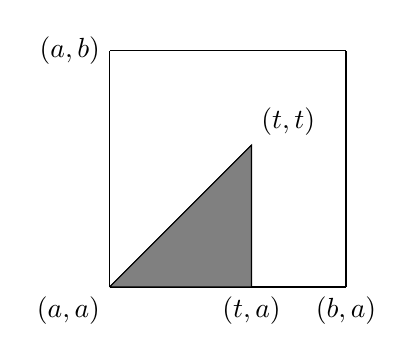
\begin{tikzpicture}[scale=3]
            \draw (0,0) -- (1,0);
            \draw (0,0) -- (0,1);
            \draw (0,1) -- (1,1);
            \draw (1,0) -- (1,1);
            \draw (0.6,0) -- (0.6,0.6);
            \draw (0,0) -- (0.6,0.6);
            \draw[fill=gray] (0,0) -- (0.6,0) -- (0.6,0.6) -- (0,0);

            \node at (0,0) [below left] {$(a,a)$};
            \node at (0,1) [left] {$(a,b)$};
            \node at (1,0) [below] {$(b,a)$};
            \node at (0.6,0) [below] {$(t,a)$};
            \node at (0.6,0.6) [above right] {$(t,t)$};
            \end{tikzpicture}
        \end{center}

        \note 我们跳过对含边界的三角形是有界闭区域的验证,这不难由定义得到。

        利用连续函数的\textbf{最值定理},最大值的确存在,因此$\varphi(x)$也存在。

        但是,为了说明$\varphi(x)$连续,我们需要证明,当右边界向右上\textbf{延伸}一段距离时,函数值的变化不会太大,这就让我们想到了本讲义10.3.3提及的一致连续性。

        \item \textbf{一致连续性证明}
        
        由于$\bar{D}$是有界闭区域,我们接下来证明,对任何$\varepsilon>0$,存在$\delta>0$使得
        $$\forall \bm{x},\bm{y}\in\bar{D},\quad|\bm{x}-\bm{y}|<\delta\Longrightarrow|f(\bm{x})-f(\bm{y})|<\varepsilon$$
        这就是多元函数的\textbf{一致连续性},证明思路与\exref{cont to inte}基本一致。
        
        我们将用到\exref{multi conv sub}的结论,任何\textbf{$\bar{D}$中的有界点列存在收敛到$\bar{D}$中的子列}。

        若一致连续性不成立,存在$\varepsilon>0$使得对任何$\delta>0$都有
        $$\exists\bm{x},\bm{y}\in\bar{D},\quad|\bm{x}-\bm{y}|<\delta,\quad|f(\bm{x})-f(\bm{y})|\ge\varepsilon$$
        对$\delta=\frac{1}{n}$取出上述的$\bm{x}$、$\bm{y}$,记为$\bm{x}_n$、$\bm{y}_n$。由于$\bm{x}_n$存在\textbf{收敛子列},设为$\bm{x}_{n_k}$,并设
        $$\lim_{k\to\infty}\bm{x}_{n_k}=\bm{x}_0$$
        由于$|\bm{x}_{n_k}-\bm{y}_{n_k}|<\frac{1}{n_k}\le\frac{1}{n}$,利用极限定义即可得到
        $$\lim_{k\to\infty}(\bm{x}_{n_k}-\bm{y}_{n_k})=\bm{0}$$
        于是
        $$\lim_{k\to\infty}\bm{y}_{n_k}=\lim_{k\to\infty}\bm{x}_{n_k}=\bm{x}_0$$
        利用\textbf{归结原理}(\exref{0 dim to m dim})即得
        $$\lim_{k\to\infty}f(\bm{y}_{n_k})=\lim_{k\to\infty}f(\bm{x}_{n_k})=f(\bm{x}_0)$$
        于是
        $$\lim_{k\to\infty}(f(\bm{y}_{n_k})-f(\bm{x}_{n_k}))=\bm{0}$$
        利用定义,这与$|f(\bm{x}_{n_k})-f(\bm{y}_{n_k})|\ge\varepsilon$恒成立矛盾,从而原命题得证。

        \item \textbf{原题证明}
        
        我们将$\varphi(t)$对应的三角形区域记为$\bar{D}_t$。当$s>t$时,$\varphi(s)$即$f$在$\bar{D}_s$上的最大值,$\varphi(t)$即$f$在$\bar{D}_t$上的最大值。
        
        \note 由于$\bar{D}_s$包含$\bar{D}_t$,可以发现$\varphi(s)\ge\varphi(t)$。另一方面,若$\varphi(s)>\varphi(t)$,可得新的最大值在$\bar{D}_s$中但不在$\bar{D}_t$中。但是,利用几何关系可以发现$\bar{D}_s$中的任何一点到$\bar{D}_t$的\textbf{最短距离}不会超过$\sqrt{2}(s-t)$,这就可以用一致性控制。

        对任何$\varepsilon>0$,取出$\delta>0$使得区域中$|\bm{x}-\bm{y}|<\delta$时$|f(\bm{x})-f(\bm{y})|<\varepsilon$。我们下面证明,当$|s-t|<\frac{\delta}{\sqrt2}$且两者均属于$[a,b]$时必然有$|\varphi(s)-\varphi(t)|<\varepsilon$。

        由对称性可设$s\ge t$,此时,若$f$在$\bar{D}_s$上的最大值在$\bar{D}_t$中,则已经得证,否则最大值点坐标必然为
        $$(\alpha,\beta),\quad\alpha\in(t,s],\quad\beta\in[a,\alpha]$$
        我们考虑点$(t,\min\{\beta,t\})$。则直接由定义可发现其与$(\alpha,\beta)$的距离的两个分量都不超过$s-t$,且它在$\bar{D}_t$中。由两分量估算可得
        $$|(\alpha,\beta)-(t,\min\{\beta,t\})|\le\sqrt{2}(s-t)<\delta$$
        于是
        $$|f(\alpha,\beta)-f(t,\min\{\beta,t\})|<\varepsilon$$
        但另一方面,由于$f(\alpha,\beta)$是$\bar{D}_s$上的最大值,$f(t,\min\{\beta,t\})$是$\bar{D}_t$上一点的值,必然有
        $$\varphi(s)=f(\alpha,\beta)\ge\varphi(t)\ge f(t,\min\{\beta,t\})$$
        此时再结合不等式即有
        $$|\varphi(s)-\varphi(t)|<\varepsilon$$
        由于我们已经对任何$\varepsilon>0$找出了$\gamma>0$使得只要$|s-t|<\gamma$且$s$、$t$都在$[a,b]$中,则$|\varphi(s)-\varphi(t)|<\varepsilon$。对每个$s$考虑$t$即可发现这符合$\varphi$连续的定义。
    \end{itemize}
}
\end{framed}

\subsubsection{应用相关}
除了之前直接考察定义的题目外,我们也可能遇到综合\textbf{各种极限定理}进行计算的问题,这里给出三个侧重方向不同的例子:
\begin{framed}
\begin{exercise}
    计算极限
    $$\lim_{(x,y)\to(0,0)}f(x,y),\quad f(x,y)=\begin{cases}\big(\frac{|xy|}{x^2+y^2}\big)^{1/x^2}&x\ne0\\0&x=0\end{cases}$$
\end{exercise}
\sol{
    \note 由于原点处沿着$x=0$方向的极限结果为0,极限若存在则只能为0,由题意需要估算证明极限为0。

    这里我们要用到一个常用的估算,也即$\frac{|xy|}{x^2+y^2}$是\textbf{有界}的,它在原点以外的点不超过$\frac{1}{2}$\ (直接由基本不等式可知),从而$x\ne0$时
    $$|f(x,y)|\le\bigg(\frac{1}{2}\bigg)^{\frac{1}{x^2}}$$
    设$r=\sqrt{x^2+y^2}$,则$r\ge x$,利用指数函数单调性可发现$x\ne0$时成立
    $$|f(x,y)|\le\bigg(\frac{1}{2}\bigg)^{\frac{1}{r^2}}$$
    由于$x=0$时$f$为0,$x=0$时上式也成立。换元得
    $$\lim_{r\to0^+}\bigg(\frac{1}{2}\bigg)^{\frac{1}{r^2}}=\lim_{s\to+\infty}\frac{1}{2^s}=0$$
    从而利用\exref{2 dim polar}知$f(x,y)$在原点的极限为0.
}
\end{framed}

\begin{framed}
\begin{exercise}
    计算极限
    $$\lim_{(x,y)\to(0,a)}f(x,y),\quad f(x,y)=\begin{cases}\frac{\sin(xy)}{x}&x\ne0\\y&x=0\end{cases}$$
\end{exercise}
\sol{
    \note 由于$(0,a)$处沿着$x=0$方向的极限结果为$a$,极限若存在则只能为0,由题意需要估算证明极限为$a$。

    \begin{itemize}
        \item \textbf{初步放缩}
        
        根据定义,我们需要估算$x\ne0$时的
        $$\frac{\sin(xy)}{x}-a$$
        也即
        $$\frac{\sin(xy)-a}{x}$$
        为了能够操作,一个自然的想法是将它拆分为\textbf{两部分},也即
        $$\bigg|\frac{\sin(xy)-a}{x}\bigg|\le\bigg|\frac{\sin(xy)-\sin(ax)}{x}\bigg|+\frac{|\sin(ax)-ax|}{|x|}$$
        第一部分利用\textbf{三角函数性质}可知不超过$\frac{|xy-ax|}{|x|}=|y-a|$。由此可知,在$x\ne0$时,我们得到了
        $$|f(x,y)-a|\le|y-a|+\frac{|\sin(ax)-ax|}{|x|}$$

        \item \textbf{估算}
        
        利用等价无穷小替换可直接算出
        $$\lim_{x\to0}\frac{\sin(ax)-ax}{x}=0$$
        接下来即是用定义估算:对任何$\varepsilon>0$,存在$\delta>0$使得
        $$\forall0<|x|<\delta,\quad\frac{|\sin(ax)-ax|}{|x|}<\frac{\varepsilon}{2}$$
        取$\delta_0=\min\{\frac{\varepsilon}{2},\delta\}$,则当$(x,y)\in\mathring{U}_\delta((0,a))$时,可发现$|x|<\delta$、$|y-a|<\delta$,当$x\ne0$时
        $$|f(x,y)-a|<\frac{\varepsilon}{2}+\frac{\varepsilon}{2}=\varepsilon$$
        当$x=0$时$|f(x,y)-a|$仅剩余$|y-a|$项,仍然满足。由于对任何$\varepsilon>0$都找到了符合要求的$\delta_0>0$,利用极限定义得
        $$\lim_{(x,y)\to(0,a)}f(x,y)=a$$
    \end{itemize}

    \note 我们事实上证明了本题中的$f$是一个\textbf{连续}函数。
}
\end{framed}

\begin{framed}
\begin{exercise}\label{multi mid to deri}
    已知$f$在$\rb$上可导且导函数\textbf{连续},计算下方极限:
    $$\lim_{(x,y)\to(t,t)}g(x,y),\quad g(x,y)=\begin{cases}\frac{f(x)-f(y)}{x-y}&x\ne y\\f'(x)&x=y\end{cases}$$
    
    若$f$在$\rb$上可导,上方极限是否一定存在?
\end{exercise}
\sol{
    \begin{itemize}
        \item \textbf{导函数连续的情况}
        
        \note 由于$(t,t)$处沿着$x=y$方向的极限结果为$f'(t)$,极限若存在则只能为$f'(t)$,由题意需要估算证明极限为$f'(t)$。

        利用\textbf{拉格朗日中值定理},在$x\ne y$时,存在$x$、$y$之间的$\xi$使得
        $$\frac{f(x)-f(y)}{x-y}=f'(\xi)$$
        由于$\xi$与$x$、$y$都有关,我们设它为$\xi(x,y)$,且$x=y$时规定$\xi(x,y)=x$,则可发现恒成立
        $$g(x,y)=f'(\xi(x,y))$$
        另一方面,由$\xi$在$x$、$y$之间(补充定义$x=y$的情况后可能含两端)可知
        $$|\xi(x,y)-t|\le\max\{|x-t|,|y-t|\}$$
        由于右侧为$x$、$y$的\textbf{初等函数}($\max\{a,b\}=\frac{a+b}{2}+\frac{|b-a|}{2}$、$|a|=\sqrt{a^2}$),利用初等函数连续性即得
        $$\lim_{(x,y)\to(t,t)}\max\{|x-t|,|y-t|\}=0$$
        再由\textbf{夹逼定理}(先得到$\xi(x,y)-t$极限为0)
        $$\lim_{(x,y)\to(t,t)}\xi(x,y)=t$$
        最后通过\textbf{复合函数极限结论},由外层函数在$t$处连续即证明了
        $$\lim_{(x,y)\to(t,t)}g(x,y)=\lim_{(x,y)\to(t,t)}f'(\xi(x,y))=f'(t)$$
        
        \item \textbf{导函数不连续的情况}
        
        我们下面证明,若$f'$在$t$处不连续,则上方极限不存在。

        由定义有
        $$\lim_{s\to t}g(s,t)=f'(t)$$
        若$f'$在$s$处不连续,下方极限
        $$\lim_{s\to t}g(s,s)=\lim_{s\to t}f'(s)$$
        一定不等于$f'(t)$,从而由\textbf{归结原理}(\exref{1 dim to m dim})可知极限不存在。
    \end{itemize}
}
\end{framed}

此外,我们也可能需要\textbf{应用连续函数性质}解决更多问题:
\begin{framed}
\begin{exercise}
    对$\rb^n$中$k>1$个不同的点$\bm{p}_1,\bm{p}_2,\dots,\bm{p}_k$,证明存在$r>0$使得半径为$r$的闭球(即对某个$\bm{x}$的$\bar{U}_{r}(\bm{x})$)能盖住所有点,但任何半径小于$r$的闭球都无法盖住所有点。
\end{exercise}
\sol{
    在任何$\bm{x}$处,由定义可发现能盖住点$\bm{p}_i$的球半径至少$|\bm{x}-\bm{p}_i|$,从而能盖住所有点的最小半径
    $$R(\bm{x})=\max_{i=1,\dots,k}|\bm{x}-\bm{p}_i|$$

    与\exref{multi mid to deri}类似,我们可以说明$r(\bm{x})$是一个\textbf{初等函数}($k$个变量的最大值可以每次取两个,取$k-1$次),从而它\textbf{连续}。不过,我们接下来要证明它在$\rb^n$中有最小值,这并不能直接由连续函数相关的定理得到。

    为了解决这个问题,我们将使用\textbf{两次取区域}的技巧:
    \begin{itemize}
        \item 我们先任取一个数,如1,则$R(\bm{x})$在$\bar{D}_1=\{\bm{x}\mid|\bm{x}|\le1\}$这个有界闭区域一定存在最小值,设为$M_0$。
        \item 接下来我们说明,只要$|\bm{x}|$充分大,$R(\bm{x})$一定会超过$M_0$。事实上,在$|\bm{x}|>M_0+|\bm{p}_1|$时,利用\textbf{三角不等式}有
        $$R(\bm{x})\ge|\bm{x}-\bm{p}_1|\ge|\bm{x}|-|\bm{p}_1|>M_0$$
        \item 现在,取$R(\bm{x})$在$\bar{D}_2=\{\bm{x}\mid|\bm{x}|\le M_0+|\bm{p}_1|+1\}$这个有界闭区域的最小值$r$。
    \end{itemize}
    我们最后证明$r$是$R$在$\rb^n$上的最小值:由于区域定义,对任何$|\bm{x}|\le M_0+|\bm{p}_1|+1$都有
    $$R(\bm{x})\ge r$$
    另一方面,对任何$|\bm{x}|>M_0+|\bm{p}_1|+1$,由之前讨论必然有
    $$R(\bm{x})\ge M_0$$
    但是,$\bar{D}_2$包含$\bar{D}_1$,因此其中的最小值只会比$\bar{D}_1$中的更小,也即$M_0\ge r$。综合就得到了证明。
}
\end{framed}

\subsection{可微性习题}
\subsubsection{定义相关}
对于可微性相关的问题,一个非常重要的学习方式是,看到一些逆命题不成立的定理,可以想一想它的\textbf{反例}该如何构造。这既可以加深我们对定理的理解,也可以让我们明白定理条件的重要性:
\begin{framed}
\begin{exercise}
    设函数
    $$f(x,y)=\begin{cases}(x^2+y^2)\sin\frac{1}{x^2+y^2}&(x,y)\ne(0,0)\\0&(x,y)=(0,0)\end{cases}$$
    证明$\partial_1f$与$\partial_2f$处处存在,且在原点不连续;$f$在原点可微。
\end{exercise}
\sol{
    \begin{itemize}
        \item \textbf{第一个偏导}
        
        直接计算可知$(x,y)\ne(0,0)$时
        $$\partial_1f(x,y)=2x\sin\frac{1}{x^2+y^2}-\frac{2x}{x^2+y^2}\cos\frac{1}{x^2+y^2}$$
        而$(x,y)=(0,0)$时由有界量乘无穷小是无穷小可知
        $$\partial_1f(0,0)=\lim_{x\to0}\frac{1}{x}\cdot x^2\sin\frac{1}{x^2}=\lim_{x\to0}x\sin\frac{1}{x^2}=0$$
        类似\exref{xm sin 1x}中的分析可知极限
        $$\lim_{t\to0}\partial_1f(t,0)=\lim_{t\to0}\bigg(2t\sin\frac{1}{t}-\frac{2}{t}\cos\frac{1}{t^2}\bigg)$$
        不存在,从而由\textbf{归结原理}(\exref{1 dim to m dim})可知$\partial_1f(x,y)$不可能在原点连续。

        \item \textbf{第二个偏导}
        直接计算可知$(x,y)\ne(0,0)$时
        $$\partial_2f(x,y)=2y\sin\frac{1}{x^2+y^2}-\frac{2y}{x^2+y^2}\cos\frac{1}{x^2+y^2}$$
        而$(x,y)=(0,0)$时由有界量乘无穷小是无穷小可知
        $$\partial_2f(0,0)=\lim_{y\to0}\frac{1}{y}\cdot y^2\sin\frac{1}{y^2}=\lim_{x\to0}x\sin\frac{1}{x^2}=0$$
        与前一部分相同可得$\partial_2f(x,y)$不在原点连续。

        \item \textbf{可微性}
        
        直接利用定义知可微等价于
        $$\lim_{(x,y)\to(0,0)}\frac{f(x,y)-f(0,0)-x\partial_1f(0,0)-y\partial_2f(0,0)}{\sqrt{x^2+y^2}}=0$$
        也即
        $$\lim_{(x,y)\to(0,0)}\sqrt{x^2+y^2}\sin\frac{1}{x^2+y^2}=0$$
        由初等函数连续性可知$\sqrt{x^2+y^2}$极限为0,类似一元时由定义可证明有界量乘无穷小是无穷小,从而上述极限的确为0,得证。
    \end{itemize}
}
\end{framed}

\begin{framed}
\begin{exercise}\label{multi dir not cont}
    设函数
    $$f(x,y)=\begin{cases}1&y=x^2,\quad x\ne0\\0&y\ne x^2\ \text{or}\ (x,y)=(0,0)\end{cases}$$
    证明$f$在0处的所有方向导数均为0,但不连续、不可微。
\end{exercise}
\sol{
    \begin{itemize}
        \item \textbf{方向导数}
        
        考虑原点处,对任何$\alpha\in\rb$,设
        $$h(t)=f(t\cos\alpha,t\sin\alpha)$$
        分类讨论:若$\cos\alpha=0$,对应$h(t)=f(0,t)=0$;若$\cos\alpha\ne0$,可发现$h(t_0)=1$当且仅当$t_0\ne0$且
        $$t_0\sin\alpha=t_0^2\cos^2\alpha$$
        也即
        $$t_0=\frac{\sin\alpha}{\cos^2\alpha}$$
        由此,$h(t)$在$(-|t_0|,|t_0|)$中恒为0。

        于是,我们证明了$f(x,y)$在\textbf{任何方向上}都在0的一个邻域恒为0,这就证明了所有方向导数均为0。

        \item \textbf{不连续不可微}
        
        直接计算有
        $$\lim_{t\to0}f(t,0)=\lim_{t\to0}0=0$$
        $$\lim_{t\to0}f(t,t^2)=\lim_{t\to0}1=1$$
        由\textbf{归结原理}(\exref{1 dim to m dim})可知$f$在原点极限不存在,因此不连续。

        由可微函数连续可知$f$在原点处不可微。
    \end{itemize}
}
\end{framed}

\begin{framed}
\begin{exercise}
    设函数
    $$f(x,y)=\begin{cases}xy\frac{x^2-y^2}{x^2+y^2}&(x,y)\ne(0,0)\\0&(x,y)=(0,0)\end{cases}$$
    证明$\partial_1\partial_2f(0,0)$与$\partial_2\partial_1f(0,0)$都存在,但不相等。
\end{exercise}
\sol{
    \begin{itemize}
        \item \textbf{第一个偏导}
        
        直接计算可知$(x,y)\ne(0,0)$时
        $$\partial_1f(x,y)=y\frac{x^2-y^2}{x^2+y^2}+xy\frac{4xy^2}{(x^2+y^2)^2}$$
        而$y=0$的直线上$f(x,y)$恒为0,于是$\partial_1f(0,0)=0$。
        
        \item \textbf{第二个偏导}
        
        直接计算可知$(x,y)\ne(0,0)$时
        $$\partial_2f(x,y)=x\frac{x^2-y^2}{x^2+y^2}+xy\frac{-4x^2y}{(x^2+y^2)^2}$$
        而$y=0$的直线上$f(x,y)$恒为0,于是$\partial_1f(0,0)=0$。
        
        \item \textbf{结果计算}
        
        由定义,利用$\partial_1f(0,0)=\partial_2f(0,0)=0$有
        $$\partial_1\partial_2f(0,0)=\lim_{x\to0}\frac{\partial_2f(x,0)}{x}=\lim_{x\to0}1=1$$
        $$\partial_2\partial_1f(0,0)=\lim_{y\to0}\frac{\partial_1f(0,y)}{y}=\lim_{y\to0}(-1)=-1$$
        两者不等。
    \end{itemize}
}
\end{framed}

\note 我们之前已经证明,若一点处$\partial_1\partial_2$与$\partial_2\partial_1$其中一个存在,另一个连续,则可以保证两者在这点相等。

\

当面对陌生的结论时,通过之前的学习积累的\textbf{估算方法}就十分重要了:
\begin{framed}
\begin{exercise}
    若$\rb^n$上的函数$f(\bm{x})$在区域$D$有定义,且存在一阶偏导数。若存在$M>0$使得
    $$\forall i=1,\dots,n,\quad\forall\bm{x}\in D,\quad|\partial_if(\bm{x})|\le M$$
    证明$f$在$D$连续。
\end{exercise}
\sol{
    由定义,对任何$\bm{x}_0\in D$存在$\delta>0$使得只要$|\bm{x}-\bm{x}_0|<\delta$就有$\bm{x}\in D$。

    此时,为了能利用偏导数条件,我们尝试进行\textbf{拆分}得到
    $$\begin{aligned}f(\bm{x})-f(\bm{x}_0)&=&&f(x_1,\dots,x_n)-f(x_{0,1},\dots,x_{0,n})\\ &=&&f(x_1,\dots,x_n)-f(x_1,\dots,x_{n-1},x_{0,n})\\ &&&+f(x_1,\dots,x_{n-1},x_{0,n})-f(x_1,\dots,x_{n-2},x_{0,n-1},x_{0,n})\\ &&&+\cdots\\ &&&+f(x_1,x_{0,2},\dots,x_{0,n})-f(x_{0,1},\dots,x_{0,n})\end{aligned}$$
    由于假设已经保证了上述每一行的两点连线段都在$D$中,对每一行利用\textbf{拉格朗日中值定理}即得存在$x_i$与$x_{0,i}$之间(此处由于两者可能相等,可能含两端)的$\xi_i$使得
    $$\begin{aligned}f(\bm{x})-f(\bm{x}_0)&=&&(x_n-x_{0,n})\partial_nf(x_1,\dots,x_{n-1},\xi_n)\\ &&&+(x_{n-1}-x_{0,n-1})\partial_{n-1}f(x_1,\dots,x_{n-1},\xi_{n-1},x_{0,n})\\ &&&+\cdots\\ &&&+(x_1-x_{0,1})\partial_1f(\xi_1,x_{0,2},\dots,x_{0,n})\end{aligned}$$
    由此可放缩为
    $$|f(\bm{x})-f(\bm{x}_0)|\le M\sum_{k=1}^n|x_k-x_{0,k}|$$
    由\textbf{初等函数连续性}可知右侧在$\bm{x}\to\bm{x}_0$时的极限为0,从而通过\textbf{夹逼定理}知左侧也为0,得证。

    \note 本题中的拆分在很多\textbf{从偏导数估算原函数}的场合都有应用。
}
\end{framed}

\subsubsection{计算相关}
偏导计算相关的大部分题目都是\textbf{并不困难}的,只是可能需要一些计算的\textbf{思路}:
\begin{framed}
\begin{exercise}
    对$\rb^3$上三阶\textbf{连续可导}的函数$f$,求函数$F$使得
    $$\frac{\partial^3f(xyz)}{\partial x\partial y\partial z}=F(xyz)$$
\end{exercise}
\sol{
    由连续可导性,我们可以以任何顺序求偏导数。直接计算得
    $$\frac{\partial}{\partial x}f(xyz)=yzf'(xyz)$$
    $$\frac{\partial}{\partial y}\frac{\partial}{\partial x}f(xyz)=zf'(xyz)+xyz^2f''(xyz)$$
    $$\frac{\partial}{\partial z}\frac{\partial}{\partial y}\frac{\partial}{\partial x}f(xyz)=f'(xyz)+3xyzf''(xyz)+x^2y^2z^2f'''(xyz)$$
    从而$F(t)=f'(t)+3tf''(t)+t^2f'''(t)$即符合要求。
}
\end{framed}

\begin{framed}
\begin{exercise}
    对$\rb$到$\rb^3$的映射$\bm{r}(t)=(x(t),y(t),z(t))$,定义其微分
    $$\dr\bm{r}(t)=(x'(t),y'(t),z'(t))\dr t$$
    证明若$x$、$y$、$z$均可微,且
    $$\forall t\in\rb,\quad|\bm{r}(t)|=1$$
    证明
    $$\forall t\in\rb,\quad\bm{r}(t)\cdot\dr\bm{r}(t)=\bm{0}\dr t$$
\end{exercise}
\sol{
    利用向量模长的定义可知条件能改写为
    $$\bm{r}(t)\cdot\bm{r}(t)=1$$
    也即
    $$x^2(t)+y^2(t)+z^2(t)=1$$
    两侧\textbf{同时对$t$求导}得
    $$2x(t)x'(t)+2y(t)y'(t)+2z(t)z'(t)=0$$
    利用定义也即
    $$2\bm{r}(t)\cdot\dr\bm{r}(t)=0\dr t$$
    两侧同除以2得最终结论。

    \note \textbf{恒等}类的条件在求导后即可转化为\textbf{导数为0}。
}
\end{framed}

\begin{framed}
\begin{exercise}
    设$f$在$\rb^2$上有连续的二阶偏导数,且方向$\bm{l}_1$、$\bm{l}_2$相互垂直,若$z=f(x,y)$,证明
    $$\bigg(\frac{\partial z}{\partial\bm{l}_1}\bigg)^2+\bigg(\frac{\partial z}{\partial\bm{l}_2}\bigg)^2=\bigg(\frac{\partial z}{\partial x}\bigg)^2+\bigg(\frac{\partial z}{\partial y}\bigg)^2$$
    $$\frac{\partial^2z}{\partial\bm{l}_1^2}+\frac{\partial^2z}{\partial\bm{l}_2^2}=\frac{\partial^2z}{\partial x^2}+\frac{\partial^2z}{\partial y^2}$$
\end{exercise}
\sol{
    由于方向导数在方向向量乘正常数后不变,可不妨设都已单位化,即
    $$\bm{l}_1=(\cos\alpha,\sin\alpha),\quad\bm{l}_2=(\cos\beta,\sin\beta)$$
    由于要证的式子关于$\bm{l}_1$、$\bm{l}_2$对称,可不妨设$\beta=\alpha+\frac{\pi}{2}$,得到
    $$\bm{l}_2=(-\sin\alpha,\cos\alpha)$$
    由此利用$f$有连续的偏导数可知\textbf{可微},从而方向导数满足
    $$\frac{\partial z}{\partial\bm{l}_1}=\cos\alpha z_x+\sin\alpha z_y$$
    $$\frac{\partial z}{\partial\bm{l}_2}=-\sin\alpha z_x+\cos\alpha z_y$$
    直接平方求和即可发现第一式成立。

    为证明第二式,由条件$z_x$、$z_y$看作$x$、$y$的函数仍然\textbf{可微},于是再求一次方向导数(利用二阶混合偏导连续则可交换,有$z_{xy}=z_{yx}$)
    $$\frac{\partial^2z}{\partial\bm{l}_1^2}=\cos\alpha\frac{\partial z_x}{\partial\bm{l}_1}+\sin\alpha\frac{\partial z_y}{\partial\bm{l}_1}=\cos^2\alpha z_{xx}+2\cos\alpha\sin\alpha z_{xy}+\sin^2\alpha z_{yy}$$
    同理
    $$\frac{\partial^2z}{\partial\bm{l}_2^2}=-\sin\alpha\frac{\partial z_x}{\partial\bm{l}_2}+\cos\alpha\frac{\partial z_y}{\partial\bm{l}_2}=\sin^2\alpha z_{xx}-2\cos\alpha\sin\alpha z_{xy}+\cos^2\alpha z_{yy}$$
    求和的结论。
}
\end{framed}

\begin{framed}
\begin{exercise}
    计算函数
    $$f(x,y)=\sin(xy)\er^{x+y}$$
    在$(0,0)$处带Peano余项的3阶泰勒展开。
\end{exercise}
\sol{
    \note 我们这里只介绍\textbf{复合函数泰勒展开}的方法,大家如果不熟练请务必\textbf{直接求导}计算。

    利用\exref{multi poly k}可以发现,展开到$xy$的$k$阶,事实上展开出了$o((x^2+y^2)^k)$,而展开到$x+y$的$k$阶则展开出了$o((x^2+y^2)^{k/2})$。

    由此,我们将$\sin(xy)$展开到\textbf{一阶},$\er^{x+y}$展开到\textbf{一阶}(由于$\sin(xy)$至少包含二次,$\er^{x+y}$只需要至多一次),通过\exref{multi comb taylor}即可得到
    $$\sin(xy)=xy+o(x^2y^2)\quad (x,y)\to(0,0)$$
    $$\er^{x+y}=1+x+y+o(x+y)\quad (x,y)\to(0,0)$$
    再次利用\exref{multi poly k}即得
    $$\sin(xy)=xy+o((x^2+y^2)^2)\quad (x,y)\to(0,0)$$
    $$\er^{x+y}=1+x+y+o(\sqrt{x^2+y^2})\quad (x,y)\to(0,0)$$
    此时,由于$o$内的函数已经在原点外的点非零,利用\exref{expand o}的推论可知此时的$o$符合\textbf{推广前定义}。

    与\exref{multi taylor peano}最后一部分相同,我们可以证明,$xyo(\sqrt{x^2+y^2})$、$o((x^2+y^2)^2)$都是$o((x^2+y^2)^{3/2})$,由此计算乘积并合并到$o((x^2+y^2)^{3/2})$中可得
    $$f(x,y)=xy+x^2y+xy^2+o((x^2+y^2)^{3/2})\quad(x,y)\to(0,0)$$

    最后,利用初等函数的导数性质,可以发现$f(x,y)$在$(0,0)$处有任意阶连续导数,从而由泰勒展开\textbf{唯一性}可知这就是符合要求的泰勒展开。
}
\end{framed}

另一个常见的问题是关于\textbf{从偏导数确定原函数},这时过程就可能更加复杂:
\begin{framed}
\begin{exercise}
    设$f$在$\rb^2$上有连续的二阶偏导数,且$z=f(x,y)$满足
    $$\frac{\partial^2z}{\partial x\partial y}=x+y+1$$
    已知$f(x,0)=x^2$、$f(0,y)=2y$,求$f$。
\end{exercise}
\sol{
    由$f$有连续的二阶偏导数可知混合偏导可交换。又由其在$\rb^2$上有定义,我们将等式看作
    $$\forall (x,y)\in\rb^2,\quad\partial_1\partial_2f(x,y)=x+y+1$$
    为了方便,我们更换记号将它写作
    $$\forall (s,t)\in\rb^2,\quad\partial_1\partial_2f(s,t)=s+t+1$$
    由于偏导连续性,两侧同时对$s$从0到$x$积分可得
    $$\int_0^x\partial_1\partial_2f(s,t)\dr s=\int_0^x(s+t+1)\dr x$$
    利用\textbf{微积分基本定理}即得
    $$\partial_2f(x,t)-\partial_2f(0,t)=\frac{x^2}{2}+tx+x$$
    再将两侧同时对0到$y$积分并利用微积分基本定理即得到
    $$(f(x,y)-f(x,0))-(f(0,y)-f(0,0))=\frac{x^2y}{2}+\frac{xy^2}{2}+xy$$
    代入即得
    $$f(x,y)=x^2+2y+\frac{x^2y}{2}+\frac{xy^2}{2}+xy$$

    \note 注意对于多元函数偏导数确定原函数的相关问题,\textbf{微积分基本定理}仍然是最本质的手段。此外,由于多元的情况相对复杂,建议大家\textbf{只用定积分}操作,过程中不要采用不定积分。
}
\end{framed}
\begin{framed}
\begin{exercise}
    设\textbf{非零}的二元函数$f$在$\rb^2$上有连续的二阶偏导数,且$z=f(x,y)$满足
    $$z\frac{\partial^2z}{\partial x\partial y}=\frac{\partial z}{\partial x}\frac{\partial z}{\partial y}$$
    证明存在一元函数$g$、$h$使得$f(x,y)=g(x)h(y)$。

    [\extra]若去除$f$非零的条件,结论是否仍然成立?
\end{exercise}
\sol{
    \begin{itemize}
        \item \textbf{$f$非零情况}
        
        \note 从\textbf{结论}入手分析:由$f(x,y)=g(x)h(y)$且$f(x,y)\ne0$可以推出$\ln|f(x,y)|=\ln|g(x)|+\ln|h(y)|$,从而$\ln|f(x,y)|$对$x$偏导再对$y$偏导后为0。

        由$f$连续且非零,根据\textbf{介值定理}可不妨设$f$恒正,若$f$恒负证明类似。

        由$f$恒非零考虑$\ln z$,由\textbf{复合函数求导公式}可知
        $$\frac{\partial}{\partial x}\ln z=\frac{1}{z}\frac{\partial z}{\partial z}$$
        $$\frac{\partial}{\partial y}\frac{\partial}{\partial x}\ln z=\frac{\partial\frac{z_x}{z}}{\partial y}=\frac{z_{xy}z-z_xz_y}{z^2}=0$$

        由此,设$p(x,y)=\ln f(x,y)$,我们事实上证明了$p$的二阶混合偏导数恒为0,此外,由条件可知$p$的两个二阶混合偏导数连续,从而必然相等。由于$p$在$\rb^2$上有定义,$\partial_1p$对第二个分量求导为0可以说明
        $$\partial_1p(x,y)=\partial_1p(x,0)+\int_0^y\partial_2\partial_1p(x,t)\dr t=\partial_1p(x,0)$$
        进一步地,由$p$的一阶偏导连续性两侧同对$x$积分可得
        $$\int_0^x\partial_1p(t,y)\dr t=\int_0^x\partial_1p(t,0)\dr t$$
        利用\textbf{微积分基本定理}后移项也即
        $$p(x,y)=p(0,y)+p(x,0)-p(0,0)$$
        记$g_0(x)=p(x,0)-p(0,0)$、$h_0(y)=p(0,y)$,则有
        $$p(x,y)=g_0(x)+h_0(y)$$
        两边同取指数得
        $$f(x,y)=\er^{g_0(x)}\er^{h_0(y)}$$
        分别记两部份为$g(x)$、$h(y)$即得结论。
        
        \item \textbf{$f$可能为0情况}
        
        结论不成立,我们考虑如下的例子:
        $$f(x,y)=\begin{cases}0&x\ge0,y\ge0\\x^3y^3&x<0\ \text{or}\ y<0\end{cases}$$
        直接计算可发现(边界处需由定义处理)
        $$\partial_1f(x,y)=\begin{cases}0&x\ge0,y\ge0\\3x^2y^3&x<0\ \text{or}\ y<0\end{cases}$$
        $$\partial_2f(x,y)=\begin{cases}0&x\ge0,y\ge0\\3x^3y^2&x<0\ \text{or}\ y<0\end{cases}$$
        $$\partial_1^2f(x,y)=\begin{cases}0&x\ge0,y\ge0\\6xy^3&x<0\ \text{or}\ y<0\end{cases}$$
        $$\partial_2^2f(x,y)=\begin{cases}0&x\ge0,y\ge0\\6x^3y&x<0\ \text{or}\ y<0\end{cases}$$
        $$\partial_2\partial_1f(x,y)=\partial_1\partial_2f(x,y)=\begin{cases}0&x\ge0,y\ge0\\9x^2y^2&x<0\ \text{or}\ y<0\end{cases}$$
        由此利用定义可知其各阶偏导连续,且可计算验证符合要求。

        但是,由于$f(1,1)=0$,若$f(x,y)=g(x)h(y)$,必然有$g(1)=0$或$h(1)=0$,从而$f(x,y)$在$x=1$或$y=1$恒为0,矛盾。

        \note 上述反例的一个构造思路如下:考虑$x$方向,则原方程即$\alpha_xz=z_x\alpha$恒成立,这里$\alpha=z_y$。若对每个$y$,$\alpha$与$z$都成比例,则几乎无法构造出反例。但是,尝试可以发现,设$g(x)=x^3$、$h(x)=\min\{x^3,0\}$,则有$g(x)h'(x)=g'(x)h(x)$,但二者不成比例。从这个思路出发,就可以考虑\textbf{分段}的反例。
    \end{itemize}
}
\end{framed}

\newpage
\section{可微的应用}
本次习题课介绍了可微的应用,也即Jacobi矩阵、隐函数定理、反函数定理、极值与条件最值,知识基础为多元函数可微性的定义与基本结论。

\note 讲义中的$\partial_1f$完全\textbf{等同于}教材中的$f_1'$,代表函数$f$对\textbf{第一个分量}的偏导数,$\partial_2$、$\partial_3$等同理;$\partial_1^2f$代表$f_{11}''$,也即对第一个分量作两次偏导数,其他同理。

\subsection{作业解答}
\note\ 6.8节的作业题中的\textbf{计算部分}可以不通过任何定理,仅通过\textbf{对特定量求偏导数}结合\textbf{解方程}得到,本节将给出对应的做法。

\begin{enumerate}
    \item (6.8节例1)已知参数$a$、$b$为正,求方程
    $$\frac{x^2}{a^2}+\frac{y^2}{b^2}=1$$
    在点$\big(\frac{a}{\sqrt2},\frac{b}{\sqrt2}\big)$附近确定的隐函数$y=f(x)$的导数,并计算$f'\big(\frac{a}{\sqrt2}\big)$。

    \sol{
        将$y$看成$f(x)$,方程两边对$x$求导得到
        $$\frac{2x}{a^2}+\frac{2yf'(x)}{b^2}=0$$
        从而解出
        $$f'(x)=-\frac{b^2x}{a^2y}$$
        代入即得$\big(\frac{a}{\sqrt2},\frac{b}{\sqrt2}\big)$处
        $$f'\bigg(\frac{a}{\sqrt2}\bigg)=-\frac{b}{a}$$

        \note 事实上,教材中的定理比起计算,更重要的是\textbf{保证能够确定可导的隐函数},而无需证明这件事时,上述的计算过程的确是\textbf{严谨}的,更多细节将在本章讨论。
    }

    \item (6.8节例2)求方程$xy+yz+\er^{xz}=3$确定的隐函数$z=f(x,y)$的偏导数$\frac{\partial z}{\partial x}$、$\frac{\partial z}{\partial y}$。
    
    \sol{
        将方程中的$z$写为$f(x,y)$,方程两边对$x$求偏导得到
        $$y+y\partial_1f(x,y)+(z+x\partial_1f(x,y))\er^{xz}=0$$
        这里第三项来自复合函数求导与乘积求导:
        $$\frac{\partial\er^{xz}}{\partial x}=\er^{xz}\frac{\partial(xz)}{\partial x}+\er^{xz}\bigg(z+x\frac{\partial z}{\partial x}\bigg)$$
        从而解出
        $$\frac{\partial z}{\partial x}=\partial_1f(x,y)=-\frac{y+z\er^{xz}}{y+x\er^{xz}}$$
        同理方程两边对$y$求偏导得到
        $$x+z+y\partial_2f(x,y)+x\partial_2f(x,y)\er^{xz}=0$$
        从而解出
        $$\frac{\partial z}{\partial y}=\partial_2f(x,y)=-\frac{x+z}{y+x\er^{xz}}$$
    }

    \item (6.8节例3)求方程$F(x-y,y-z)=0$确定的隐函数$z=f(x,y)$的偏导数$\frac{\partial z}{\partial x}$、$\frac{\partial z}{\partial y}$。
    
    \sol{
        将方程中的$z$写为$f(x,y)$,方程两边对$x$求偏导得到
        $$\partial_1F(x-y,y-z)\frac{\partial(x-y)}{\partial x}+\partial_2F(x-y,y-z)\frac{\partial(y-z)}{\partial x}=0$$
        也即
        $$\partial_1F(x-y,y-z)-\partial_2F(x-y,y-z)\partial_1f(x,y)=0$$
        从而解出
        $$\frac{\partial z}{\partial x}=\partial_1f(x,y)=\frac{\partial_1F(x-y,y-z)}{\partial_2F(x-y,y-z)}$$
        方程两边对$y$求偏导得到
        $$\partial_1F(x-y,y-z)\frac{\partial(x-y)}{\partial y}+\partial_2F(x-y,y-z)\frac{\partial(y-z)}{\partial y}=0$$
        也即
        $$-\partial_1F(x-y,y-z)+(1-\partial_1f(x,y))\partial_2F(x-y,y-z)=0$$
        从而解出
        $$\frac{\partial z}{\partial x}=\partial_1f(x,y)=\frac{\partial_2F(x-y,y-z)-\partial_1F(x-y,y-z)}{\partial_2F(x-y,y-z)}$$
    }
    
    \item (6.8节例4)求方程$\er^x\sin y+yz+\er^z+5=0$确定的隐函数$z=f(x,y)$的偏导数$\frac{\partial z}{\partial x}$、$\frac{\partial^2z}{\partial x\partial y}$。
    
    \sol{
        \note 注意第二个记号表示\textbf{从左到右},先对$x$求偏导再对$y$求偏导,它并不等于需要\textbf{从右到左}计算的$\frac{\partial}{\partial x}\frac{\partial z}{\partial y}$。

        将方程中的$z$写为$f(x,y)$,方程两边对$x$求偏导得到
        $$\er^x\sin y+y\partial_1f(x,y)+\er^z\partial_1f(x,y)=0$$
        从而解出
        $$\frac{\partial z}{\partial x}=\partial_1f(x,y)=-\frac{\er^x\sin y}{y+\er^z}$$
        将上式右侧的$z$看作$f(x,y)$,将$x$视作常数对$y$求偏导可得
        $$\frac{\partial^2z}{\partial x\partial y}=-\frac{\er^x\cos y(y+\er^z)-\frac{\partial(y+\er^z)}{\partial y}\er^x\sin y}{(y+\er^z)^2}$$
        进一步计算即得
        $$\frac{\partial^2z}{\partial x\partial y}=\er^x\frac{\sin y(1+\er^z\partial_2f(x,y))-\cos y(y+\er^z)}{(y+\er^z)^2}$$
        由此我们需要计算$\partial_2f(x,y)$。将原方程两边对$y$求偏导得到
        $$\er^x\cos y+z+y\partial_2f(x,y)+\er^z\partial_2f(x,y)=0$$
        从而解出
        $$\partial_2f(x,y)=-\frac{\er^x\cos y+z}{y+\er^z}$$
        代入最终得到
        $$\frac{\partial^2z}{\partial x\partial y}=\er^x\frac{\sin y(y+\er^z-\er^z(\er^x\cos y+z))-\cos y(y+\er^z)^2}{(y+\er^z)^3}$$
    }
    
    \item (6.8节例5)确定所有的点$(x_0,y_0)$使得方程组
    $$\begin{cases}x^2+y^2-uv=0\\xy+u^2-v^2=0\end{cases}$$
    能在$(x_0,y_0)$附近确定可导的隐函数$u=f(x,y)$、$v=g(x,y)$,并求此时它们的各偏导数$u_x$、$u_y$、$v_x$、$v_y$\ (这里下标即表示偏导)。
    
    \sol{
        \begin{itemize}
            \item \textbf{存在性}
            
            设两个方程为$F(x,y,u,v)=G(x,y,u,v)=0$,直接计算Jacobi行列式可知
            $$\frac{D(F(x,y,u,v),G(x,y,u,v))}{D(u,v)}=\begin{vmatrix}-v&-u\\2u&-2v\end{vmatrix}=2(u^2+v^2)$$
            直接计算可发现$2(u^2+v^2)=0$可推出$u=v=0$,从而此时必须$x=y=0$,通过隐函数存在定理(由定义可发现连续性条件满足),只要$(x_0,y_0)$处方程组有解$(u_0,v_0)$且$(x_0,y_0)\ne(0,0)$,即可在$(x_0,y_0)$附近确定满足$(f(x_0,y_0),g(x_0,y_0))=(u_0,v_0)$的隐函数。

            \note 当写出Jacobi行列式时,默认\textbf{``分母''中的量相匹配},本题中即$u$、$v$相匹配。
            
            \item \textbf{偏导计算}
            
            在$(x_0,y_0)\ne(0,0)$附近,将$u$、$v$看作$f(x,y)$、$g(x,y)$,两方程同时对$x$求偏导可得
            $$\begin{cases}2x-u_xv-uv_x=0\\y+2uu_x-2vv_x=0\end{cases}$$
            从而解得
            $$u_x=\frac{4xv-yu}{2(u^2+v^2)},\quad v_x=\frac{4xu+yv}{2(u^2+v^2)}$$
            同理,两方程同时对$y$求偏导可得
            $$\begin{cases}2y-u_yv-uv_y=0\\x+2uu_y-2vv_y=0\end{cases}$$
            从而解得
            $$u_y=\frac{4yv-xu}{2(u^2+v^2)},\quad v_y=\frac{4yu+xv}{2(u^2+v^2)}$$

            \note 可以发现,某种意义上可以直接从\textbf{形式计算后分母非零}(此处即$2(u^2+v^2)\ne0$)得到存在性条件。
        \end{itemize}
    }

    \item (6.8节例6)求方程组
    $$\begin{cases}x=\er^u+v\\xy=\er^u+u\end{cases}$$
    确定的隐函数$u=f(x,y)$、$v=g(x,y)$的偏导数$u_x$、$u_{xx}$。

    \sol{
        将$u$、$v$看作$f(x,y)$、$g(x,y)$,两方程同时对$x$求偏导可得
        $$\begin{cases}1=\er^uu_x+v_x\\y=\er^uu_x+u_x\end{cases}$$
        从而解得
        $$u_x=\frac{y}{\er^u+1}$$
        将上式右侧的$u$看作$f(x,y)$,继续对$x$求偏导,利用复合函数导数公式即得到
        $$u_{xx}=-\frac{y}{(\er^u+1)^2}\er^uu_x$$
        代入$u_x$表达式即得结果为
        $$u_{xx}=-\frac{\er^uy^2}{(\er^u+1)^3}$$
    }
    
    \item (6.8节例7)证明极坐标变换
    $$\begin{cases}x=r\cos\theta\\y=r\sin\theta\end{cases}$$
    的Jacobi行列式满足$\frac{D(x,y)}{D(r,\theta)}=r$。

    \sol{
        直接计算Jacobi行列式可知
        $$\frac{D(x,y)}{D(r,\theta)}=\begin{vmatrix}\cos\theta&-r\sin\theta\\\sin\theta&r\cos\theta\end{vmatrix}=r(\cos^2\theta+\sin^2\theta)=r$$
    }

    \item (6.8节例8)求方程组
    $$\begin{cases}u^2-v=3x+y\\u-2v^2=x-2y\end{cases}$$
    确定的隐函数$u=f(x,y)$、$v=g(x,y)$的偏导数$u_x$、$v_x$。

    \sol{
        将$u$、$v$看作$f(x,y)$、$g(x,y)$,两方程同时对$x$求偏导可得
        $$\begin{cases}2uu_x-v_x=3\\u_x-4vv_x=1\end{cases}$$
        从而解得($8uv\ne1$时)
        $$u_x=\frac{12v-1}{8uv-1},\quad v_x=\frac{2u-3}{8uv-1}$$

        \note 与一元时类似,仅\textbf{计算结果}时无需讨论分母为0时会如何。
    }

    \item (6.8节例9)证明球坐标变换
    $$\begin{cases}x=r\cos\theta\sin\varphi\\y=r\sin\theta\sin\varphi\\z=r\cos\varphi\end{cases}$$
    的Jacobi行列式满足$\frac{D(x,y,z)}{D(r,\varphi,\theta)}=r^2\sin\varphi$。

    \note 不同的变量顺序将导致Jacobi行列式\textbf{相差符号},因此对应计算必须\textbf{指定顺序}。

    \sol{
        直接按最后一行展开计算Jacobi行列式可知
        $$\frac{D(x,y,z)}{D(r,\varphi,\theta)}=\begin{vmatrix}\cos\theta\sin\varphi&r\cos\theta\cos\varphi&-r\sin\theta\sin\varphi\\\sin\theta\sin\varphi&r\sin\theta\cos\varphi&r\cos\theta\sin\varphi\\\cos\varphi&-r\sin\varphi&0\end{vmatrix}=r^2\cos^2\varphi\sin\varphi+r^2\sin^3\varphi=r^2\sin\varphi$$
    }
    
    \item (习题6.8.10)求方程组
    $$\begin{cases}x=\cos\varphi\cos\theta\\y=\cos\varphi\sin\theta\\z=\sin\varphi\end{cases}$$
    确定的隐函数$z=f(x,y)$的偏导数$z_x$。

    \sol{
        由条件可知需要将$\theta$、$\varphi$、$z$\textbf{都看作}$x$、$y$的函数,三方程同时对$x$求偏导可得
        $$\begin{cases}1=-\varphi_x\sin\varphi\cos\theta-\theta_x\cos\varphi\sin\theta\\0=-\varphi_x\sin\varphi\sin\theta+\theta_x\cos\varphi\cos\theta\\z_x=\varphi_x\cos\varphi\end{cases}$$
        第一式乘$\cos\theta$加第二式乘$\sin\theta$可得
        $$\cos\theta=-\varphi_x\sin\varphi$$
        从而代入第二式即得($\tan\varphi\ne0$时)
        $$z_x=-\frac{\cos\theta}{\tan\varphi}$$

        \note 确定某个量为$x$、$y$的隐函数意味着所有量都要看作$x$、$y$的隐函数。
    }

    \item (习题6.8.11)设函数$f$、$g$、$a$、$b$在$\rb^2$上有连续的一阶偏导数,且
    $$u=f(x,y),\quad v=g(x,y),\quad x=a(\xi,\eta),\quad y=b(\xi,\eta)$$
    证明
    $$\frac{D(u,v)}{D(\xi,\eta)}=\frac{D(u,v)}{D(x,y)}\cdot\frac{D(x,y)}{D(\xi,\eta)}$$

    \sol{
        利用定义可知等式左侧为
        $$u_\xi v_\eta-u_\eta v_\xi$$
        由复合函数求导公式可知
        $$u_\xi=u_xx_\xi+u_yy_\xi,\quad v_\xi=v_xx_\xi+v_yy_\xi$$
        $$u_\eta=u_xx_\eta+u_yy_\eta,\quad v_\eta=v_xx_\eta+v_yy_\eta$$
        由此直接展开计算验证可知
        $$\begin{aligned}u_\xi v_\eta-u_\eta v_\xi&=(u_xx_\xi+u_yy_\xi)(v_xx_\eta+v_yy_\eta)-(v_xx_\xi+v_yy_\xi)(u_xx_\eta+u_yy_\eta)\\ &=u_xv_yx_\xi y_\eta+u_yv_xy_\xi x_\eta+u_yv_xx_\xi y_\eta-v_yu_xy_\xi x_\eta\\ &=(u_xv_y-v_xu_y)(x_\xi y_\eta-x_\eta y_\xi)\end{aligned}$$
        从而再由右侧定义得结论成立。
    }

    \item (6.9节例4)求$\rb^2$上的函数
    $$f(x,y)=x^4+y^4-x^2-2xy-y^2$$
    的稳定点,并判定是否是极值点。

    \sol{
        直接计算可知
        $$\partial_1f(x,y)=4x^3-2x-2y,\quad\partial_2f(x,y)=4y^3-2x-2y$$
        由此可知稳定点当且仅当$4x^3-2x-2y=4y^3-2x-2y=0$,两式相减可知$4x^3=4y^3$,从而$x=y$,进一步解得稳定点有$(-1,-1)$、$(0,0)$与$(1,1)$。

        进一步计算有
        $$\partial_1^2f(x,y)=12x^2-2,\quad\partial_1\partial_2f(x,y)=\partial_2\partial_1f(x,y)=-2,\quad\partial_2^2f(x,y)=12y^2-2$$
        从而计算可知$(-1,-1)$与$(1,1)$处$A>0$、$B^2-AC<0$,$(-1,-1)$与$(1,1)$处为极小值点。
        
        虽然$(0,0)$处$A<0$,但由于$B^2=AC$,无法直接通过此方法判别。不过,在直线$x=0$上,$f(x,y)=y^4-y^2=y^2(y^2-1)$,在0附近小于0;在直线$y=-x$上,$f(x,y)=2x^4$,在0附近大于0。由此,$(0,0)$并不是$f(x,y)$的极值点。

        \note 一般来说,无法判别时往往需要通过\textbf{找不同路径}证明不为极值点。
    }

    \item (习题6.9.1(5))求$\rb^2$上的函数
    $$f(x,y)=x^3y^2(6-x-y)$$
    在$x>0$、$y>0$中的极值。

    \sol{
        直接计算可知
        $$\partial_1f(x,y)=3x^2y^2(6-x-y)-x^3y^2,\quad\partial_2f(x,y)=2x^3y(6-x-y)-x^3y^2$$
        由此可知稳定点当且仅当$3x^2y^2(6-x-y)=x^3y^2=2x^3y(6-x-y)$,由$x>0$、$y>0$,化简可得
        $$\begin{cases}3(6-x-y)=x\\y=2(6-x-y)\end{cases}$$
        由此可解得$x=3$、$y=2$,进一步计算二阶导数可发现
        $$\partial_1^2f(x,y)=36xy^2-12x^2y^2-6xy^3$$
        $$\partial_1\partial_2f(x,y)=\partial_2\partial_1f(x,y)=36x^2y-8x^3y-9x^2y^2$$
        $$\partial_2^2f(x,y)=12x^3-2x^4-6x^3y$$
        于是
        $$\partial_1^2f(3,2)=-144,\quad\partial_1\partial_2f(3,2)=\partial_2\partial_1f(3,2)=-108,\quad\partial_2^2f(3,2)=-162$$
        由此$(3,2)$处$A<0$、$B^2-AC<0$,从而其为极大值点。
    }
    
    \item (习题6.9.3)求函数
    $$H(x,y,z)=6x-y^2+xz+60$$
    在球面$x^2+y^2+z^2=36$上的最小值点。

    \sol{
        构造辅助函数
        $$F(x,y,z,\lambda)=6x-y^2+xz+60+\lambda(x^2+y^2+z^2-36)$$
        求导可得方程组
        $$\begin{cases}\partial_1F(x,y,z,\lambda)=6+z+2x\lambda=0\\\partial_2F(x,y,z,\lambda)=-2y+2y\lambda=0\\\partial_3F(x,y,z,\lambda)=x+2z\lambda=0\\x^2+y^2+z^2=36\end{cases}$$
        第二式可得$y=0$或$\lambda=1$,代入$\lambda=1$可解得$(x,y,z)=(-4,\pm4,2)$,代入$y=0$可解得(先代入$x=-2z\lambda$,再消去$\lambda$)\ $(x,y,z)=(0,0,-6)$或$(x,y,z)=(\pm3\sqrt3,0,3)$。

        进一步计算可发现,五个稳定点处$H(x,y,z)$的值分别为12、12、60、$60\pm18\sqrt{3}$。比较可知其中最小的是12,由此若球面上的最小值存在可知最小值点为$(-4,\pm4,2)$,对应最小值12。

        \note 这类问题一般\textbf{无需严谨证明},只要\textbf{说明}对应的稳定点为最值点即可。对本题来说,通过数学分析知识可以证明球面上的连续函数一定存在最小值点,因此稳定点中值最小的就是最小值点。
    }

    \item (习题6.9.5)求平面$y+2z=12$与$x+y=6$的交线上与原点最近的点。
    
    \sol{
        与原点距离即$\sqrt{x^2+y^2+z^2}$,考虑其平方,设$f(x,y,z)=x^2+y^2+z^2$,问题即在两个约束的前提下求$f$的最小值点,构造辅助函数
        $$F(x,y,z,\lambda,\mu)=x^2+y^2+z^2+\lambda(y+2z-12)+\mu(x+y-6)$$
        求导可得方程组
        $$\begin{cases}2x+\mu=0\\2y+\lambda+\mu=0\\2z+2\lambda=0\\y+2z=12\\x+y=6\end{cases}$$
        利用线性方程组知识可得到唯一解$(x,y,z)=(2,4,4)$,此时$\mu=-4$、$\lambda=-4$。根据几何关系,直线上到给定点最近的点\textbf{一定存在}(为点到直线作垂线的垂足),因此唯一的稳定点$(2,4,4)$即为所求的最近的点。
    }

    \item (习题6.9.8)当$n$个正数$x_1,x_2,\dots,x_n$的和等于常数$l>0$时,求它们乘积的最大值。由此证明对任何正数$a_1,\dots,a_n$满足
    $$\sqrt[n]{a_1\dots a_n}\le\frac{a_1+\dots+a_n}{n}$$
    
    \sol{
    \begin{itemize}
        \item \textbf{乘子构造}
        
        构造辅助函数
        $$F(x_1,\dots,x_n,\lambda)=x_1x_2\dots x_n+\lambda(x_1+\dots+x_n-l)$$
        对每个$x_i$求导可得(这里$\prod_{j\ne i}x_j$代表除了$x_i$以外的其他所有$x_j$乘积)
        $$\forall i=1,\dots,n,\quad\prod_{j\ne i}x_j+\lambda=0$$
        由于$x_i$均为正数,设$M=x_1\dots x_n$,则可知
        $$\forall i=1,\dots,n,\quad\frac{M}{x_i}+\lambda=0$$
        也即所有$x_i$均等于$-\frac{\lambda}{M}$,这就得到$x_i$均正的稳定点只有
        $$x_1=x_2=\dots=x_n=\frac{l}{n}$$
        此时乘积值为$\frac{l^n}{n^n}$。

        \item \textbf{最大值说明}
        
        \note 本部分\textbf{并非严谨证明},仅为一个让大家理解为何其为最大值的说明,事实上其证明远远超出了这门课的知识范围。

        考虑集合
        $$\bar{D}=\{\bm{x}\in\rb^n\mid x_1+\dots+x_n=l,\quad x_1\ge0,\quad\dots,\quad,x_n\ge0\}$$
        由于$x_1+\dots+x_n=l$在$\rb^n$中构成了一个$n-1$维的超平面,而$x_1\ge0$到$x_n\ge0$划分出了其中有界的部分(所有$x_i$都在$[0,l]$中),且边界封闭,$\bar{D}$可以\textbf{等同于}$\rb^{n-1}$中的有界闭区域。

        \note 可以考虑$n=2$、$n=3$的情况帮助理解。

        由于$f(x_1,\dots,x_n)=x_1\dots x_n$是$\bar{D}$上的连续函数,利用有界闭区域上的连续函数有最大值,可知$f$在$\bar{D}$上必然\textbf{有最大值}。在$\bar{D}$的边界上,必然有某个$x_i$为0,因此$f$为0,而内部$f$恒大于0,于是最大值\textbf{不可能在边界上}。
        
        进一步地,由$f$的可微性,内部的最大值\textbf{必然在稳定点},上一部分找到的$x_1=x_2=\dots=x_n=\frac{l}{n}$是其内部的唯一稳定点,也就对应着唯一的最大值
        $$f(x_1,\dots,x_n)=\frac{l^n}{n^n}$$
        
        \item \textbf{均值不等式}
        
        对任意$n$个整数$a_1,\dots,a_n$,设$L=a_1+\dots+a_n$,由前两部分证明可知必然有
        $$a_1\dots a_n\le\frac{L^n}{n^n}$$
        两边同取$n$次方根并代入$L=a_1+\dots+a_n$即得结论。

        \note 这也是不等式的一种证明方法,也即\textbf{固定一侧后让另一侧尽量大/小}。
    \end{itemize}
    }
\end{enumerate}

\subsection{隐函数与反函数}
本节中我们将介绍一系列有关\textbf{多元可微映射}的结论。由于其中的大部分结论需要复杂的\textbf{微分几何}讨论,我们将跳过证明部分。

\subsubsection{Jacobi矩阵}
在介绍多元函数的极限与连续性时,我们一直都将结论推广到了\textbf{多元映射}中,本部分我们就将把多元函数\textbf{可微性}的相关结论推广至多元映射。

考虑$n$维到$m$维的映射$\bm{F}(\bm{x})=(F_1(\bm{x}),\dots,F_m(\bm{x}))$,若它的\textbf{每个分量}都在$\bm{x}$处存在各一阶偏导数,则称$\bm{F}$在$\bm{x}$处存在各一阶偏导数。同理,称它\textbf{可微}当且仅当\textbf{每个分量都可微}。

对于多元函数来说,表达它对各个分量的偏导数需要一个\textbf{向量},对于多元映射,也就自然需要一个$m\times n$的\textbf{矩阵}(用最简单的语言说,就是将数排成\textbf{$m$行$n$列})。我们称
$$J_{\bm{F}}(\bm{x})=\begin{pmatrix}\partial_1F_1(\bm{x})&\partial_2F_1(\bm{x})&\cdots&\partial_nF_1(\bm{x})\\\partial_1F_2(\bm{x})&\partial_2F_2(\bm{x})&\cdots&\partial_nF_2(\bm{x})\\\vdots&\vdots&\ddots&\vdots\\\partial_1F_m(\bm{x})&\partial_2F_m(\bm{x})&\cdots&\partial_nF_m(\bm{x})\end{pmatrix}$$
为$\bm{F}$在$\bm{x}$处的\textbf{Jacobi矩阵},当$\bm{F}$在$\bm{x}$存在一阶偏导数时可定义。可以发现,它的第一行就是$F_1$的梯度,第二行就是$F_2$的梯度,以此类推,第$i$行第$j$列为$\partial_jF_i(\bm{x})$。

\

我们用两个结论来说明Jacobi矩阵的\textbf{几何意义}:
\begin{framed}
\begin{exercise}
    设$\bm{F}(\bm{x})=A\bm{x}$,这里$\bm{x}\in\rb^n$为\textbf{列向量},$A\in\rb^{m\times n}$为\textbf{矩阵},证明
    $$\forall\bm{x}\in\rb^n,\quad J_{\bm{F}}(\bm{x})=A$$
\end{exercise}
\sol{
    利用矩阵乘法定义可知
    $$(A\bm{x})_i=\sum_{k=1}^na_{ik}x_k$$
    从而即有
    $$\partial_jF_i(\bm{x})=\frac{\partial(A\bm{x})_i}{\partial x_j}=a_{ij}$$
    再利用Jacobi矩阵定义得结论。
}
\end{framed}

\begin{framed}
\begin{exercise}
    考虑$n$维到$m$维的映射$\bm{F}$\ (看成\textbf{列向量到列向量的映射}),若对$\bm{x}\in\rb^n$,$\bm{F}$在$\bm{x}$处可微,则
    $$\bm{F}(\bm{x}+\bm{h})=\bm{F}(\bm{x})+J_{\bm{F}}(\bm{x})\bm{h}+o(|\bm{h}|)\quad(\bm{h}\to\bm{0})$$
    这里$o(|\bm{h}|)$代表一个每个分量都为$o(|\bm{h}|)$的向量。
\end{exercise}
\sol{
    由可微定义可知对任何$i=1,\dots,m$有
    $$F_i(\bm{x}+\bm{h})=F_i(\bm{x})+\bm{h}\cdot\nabla F_i(\bm{x})+o(|\bm{h}|)\quad(\bm{h}\to\bm{0})$$
    即
    $$F_i(\bm{x}+\bm{h})=F_i(\bm{x})+\sum_{j=1}^n\partial_jF_i(\bm{x})h_j+o(|\bm{h}|)\quad(\bm{h}\to\bm{0})$$
    利用矩阵乘法定义即可知将所有$i$拼成一列得到的就是题中要证的目标。
}
\end{framed}
由此可见,Jacobi矩阵几乎对应着一元函数的导数,代表一个可微的映射在一点附近的\textbf{线性近似系数}——对一元函数也就是\textbf{切线斜率}。

若$m=n$,对应的Jacobi矩阵是\textbf{方阵},由此它可以计算行列式,称为\textbf{Jacobi行列式}。正如行列式的几何意义是变换$\bm{x}\to A\bm{x}$将\textbf{有向体积}改变的倍数,Jacobi行列式的值就对应原本的$n$维空间一点附近的\textbf{体积元}被放大的倍数。我们下学期介绍多元积分时还将再次提及这个概念,来进行多元积分的\textbf{换元}。

\

有了Jacobi矩阵与矩阵运算后,\textbf{复合函数求导公式}可以重新写成简洁的形式,与一元函数几乎一致:
\begin{framed}
\begin{exercise}
    考虑$n$维到$m$维的\textbf{可微}映射$\bm{F}$,$p$维到$n$维一阶可导的映射$\bm{G}$,设$p$维到$m$维的映射$\bm{H}(\bm{x})=\bm{F}(\bm{G}(\bm{x}))$\ (也即$\bm{H}$为$\bm{F}$与$\bm{G}$的复合),则
    $$\bm{J}_{\bm{H}}(\bm{x})=J_{\bm{F}}(\bm{G}(\bm{x}))J_{\bm{G}}(\bm{x})$$
\end{exercise}
\sol{
    根据定义可知对任何$i=1,\dots,m$有
    $$H_i(\bm{x})=F_i(\bm{G}(\bm{x}))$$
    利用\textbf{复合函数求导公式}可直接得到导函数为
    $$\partial_jH_i(\bm{x})=\sum_{k=1}^n\partial_kF_i(\bm{G}(\bm{x}))\partial_jG_k(\bm{x})$$
    结合矩阵乘法与Jacobi矩阵的定义即得结论。
}
\end{framed}

除了函数以外,我们也可以考虑\textbf{向量表达式}的Jacobi矩阵。设向量$\bm{z}=(z_1,\dots,z_m)$的每个分量都是$x_1,\dots,x_n$的表达式。记
$$\frac{D\bm{z}}{D\bm{x}}=\begin{pmatrix}\frac{\partial z_1}{\partial x_1}&\frac{\partial z_1}{\partial x_2}&\cdots&\frac{\partial z_1}{\partial x_n}\\\frac{\partial z_2}{\partial x_1}&\frac{\partial z_2}{\partial x_2}&\cdots&\frac{\partial z_2}{\partial x_n}\\\vdots&\vdots&\ddots&\vdots\\\frac{\partial z_m}{\partial x_1}&\frac{\partial z_m}{\partial x_2}&\cdots&\frac{\partial z_m}{\partial x_n}\end{pmatrix}$$
表示将$\bm{z}$的每个分量都看作包含$\bm{x}$的表达式后求所有偏导的结果。

可以发现,在此定义下,我们可以将向量表达式的\textbf{微分}写作
$$\dr\bm{z}=\frac{D\bm{z}}{D\bm{x}}\dr\bm{x}$$
这里$\dr\bm{z}=(\dr z_1,\dots,\dr z_m)^\top$、$\dr\bm{x}=(\dr z_1,\dots,\dr x_n)^\top$均为\textbf{列向量},直接对比每个分量即可由多元函数的全微分定义知其相等。此外,表达式的复合函数求导公式可以写成
$$\frac{D\bm{z}}{D\bm{x}}=\frac{D\bm{z}}{D\bm{y}}\frac{D\bm{y}}{D\bm{x}}$$
由此可证明向量表达式的一阶微分\textbf{仍然具有形式不变性}。

\subsubsection{隐函数定理}
首先,我们来表述一般情况的\textbf{隐函数定理}。考虑一个$n$维到$m$维($n>m$)的映射$\bm{F}$,并考虑它对应的方程组
$$\bm{F}(\bm{x})=\bm{0}$$
由于这实际上是$n$个未知数、$m$个方程,从直觉上来说,我们应当可以保留$n-m$个自由变量,将其他都看成这些自由变量的函数。

隐函数定理的具体形式是,给出$\bm{x}$中的$m$个\textbf{分量}$I=\{i_1,\dots,i_m\}$,我们记其中未出现的分量集合为$I^c=\{j_1,\dots,j_{n-m}\}$,并记
$$\bm{x}_I=(x_{i_1},\dots,x_{i_m}),\quad\bm{x}_{I^c}=(x_{j_1},\dots,x_{j_{n-m}})$$
$$\bm{x}_I\oplus\bm{x}_{I^c}=\bm{x}$$

若$\bm{F}(\bm{x}_0)=\bm{0}$且$\bm{F}$在$\bm{x}_0$附近\textbf{一阶偏函数连续},考虑$J_{\bm{F}}(\bm{x}_0)$的第$i_1,\dots,i_m$列构成的\textbf{方阵}$J_{\bm{F}}^I(\bm{x}_0)$,假设
$$\det J_{\bm{F}}^I(\bm{x}_0)\ne0$$
则在$(\bm{x}_0)_{I^c}$某邻域\textbf{存在唯一}$n-m$维到$m$维的\textbf{一阶偏函数连续}的映射$\bm{\varphi}$,使得
$$\bm{\varphi}((\bm{x}_0)_{I^c})=(\bm{x}_0)_I,\quad\bm{F}(\bm{\varphi}(\bm{t})\oplus\bm{t})=\bm{0}$$
且$\bm{\varphi}$在$(\bm{x}_0)_{I^c}$附近\textbf{一阶偏导数连续}。

\

虽然此处完整的表述非常\textbf{复杂},但大家只要跟着教材操作过几个例子,一定能够理解对于具体的函数应当如何确定。我们现在尝试对它进行一些注释:
\begin{itemize}
    \item 首先,给定的$\bm{x}$中的$m$个分量集合,是我们确定希望作为\textbf{因变量}的分量$\bm{x}_I$,剩下的$n-m$个自由变量$\bm{x}_{I^c}$是作为\textbf{自变量}存在的。
    \item 定义$\bm{x}_I\oplus\bm{x}_{I^c}=\bm{x}$的含义是,$\oplus$符号代表我们将因变量、自变量\textbf{重新排列回}$x_1,\dots,x_n$,一方便操作。
    \item $\bm{F}(\bm{x}_0)=0$代表我们找到了一个\textbf{满足方程的点},只有在一点附近确定的函数才有意义。
    \item 接下来这步,为何我们需要条件$\det J_{\bm{F}}^I(\bm{x}_0)\ne0$?考虑$m=1$、$n=2$时,此条件事实上就成为了$F$对\textbf{因变量的偏导}非0。利用导函数的\textbf{连续性}$F$对因变量的偏导非零可以推出局部\textbf{单调},这就说明\textbf{局部}对同一个自变量,不会有两个因变量都满足方程。
    \item 在满足这些条件以后,我们就能确定一个自变量到因变量的函数$\bm{\varphi}$了,它自然是$n-m$维到$m$维的。
    \item $\bm{\varphi}$的第一条性质是说,既然它是在$\bm{x}_0$附近找到的,至少自变量与因变量需要过$\bm{x}_0$这点。
    \item $\bm{\varphi}$的第二条性质是说,既然它是由$\bm{F}(\bm{x})=\bm{0}$确定的函数,将自变量与因变量代入$\bm{F}$,当然应该得到$\bm{0}$。
    \item 最后,$\bm{\varphi}$是具有连续的一阶偏导数的,我们马上就将看到如何进行计算。
\end{itemize}

\

接下来,我们先看一个具体的例子,再进行一个相对复杂的计算:
\begin{framed}
\begin{exercise}
    设$y=f(x,t)$,且$x$、$y$、$t$满足方程$F(x,y,t)=0$。若$f$、$F$均有连续的一阶偏导数,确定可以计算$\frac{\dr y}{\dr x}$的条件,并计算$\frac{\dr y}{\dr x}$。
\end{exercise}
\sol{
    此题的表述虽然看起来非常复杂,但本质上我们其实有两个方程
    $$y=f(x,t),\quad F(x,y,t)=0$$
    利用隐函数定理,两个方程应当对应两个\textbf{因变量},这道题计算$\frac{\dr y}{\dr x}$本质上是将$x$看作了\textbf{唯一的自变量},由此$y$、$t$都是因变量。

    将第一个方程$y-f(x,t)=0$,对$y$求偏导得到1,对$t$求偏导得到$-\partial_2f(x,t)$;第二个方程对$y$求偏导得到$\partial_2F(x,y,t)$,对$t$求偏导得到$\partial_3F(x,y,t)$。

    由此,Jacobi矩阵中对应的两列拼成的矩阵应当为
    $$\begin{pmatrix}1&-\partial_2f(x,t)\\\partial_2F(x,y,t)&\partial_3F(x,y,t)\end{pmatrix}$$
    于是当行列式
    $$\partial_3F(x,y,t)+\partial_2f(x,t)\partial_2F(x,y,t)\ne0$$
    时,能在满足方程的$x,y,t$附近确定$y$、$t$为$x$的函数。

    此时,我们对两个方程分别计算对$x$的导数(将$y$、$t$都看作$x$的函数),可以发现
    $$y_x-\partial_1f(x,t)-\partial_2f(x,t)t_x=0,\quad\partial_1F(x,y,t)+\partial_2F(x,y,t)y_x+\partial_3F(x,y,t)t_x=0$$
    也即
    $$\begin{pmatrix}1&-\partial_2f(x,t)\\\partial_2F(x,y,t)&\partial_3F(x,y,t)\end{pmatrix}\begin{pmatrix}y_x\\t_x\end{pmatrix}=-\begin{pmatrix}-\partial_1f(x,t)\\\partial_1F(x,y,t)\end{pmatrix}$$
    可以发现,此时的系数矩阵恰好就是之前判断行列式非零的矩阵,而矩阵行列式非零则可逆,由此可直接解出
    $$\begin{pmatrix}y_x\\t_x\end{pmatrix}=-\begin{pmatrix}1&-\partial_2f(x,t)\\\partial_2F(x,y,t)&\partial_3F(x,y,t)\end{pmatrix}^{-1}\begin{pmatrix}-\partial_1f(x,t)\\\partial_1F(x,y,t)\end{pmatrix}$$
    简便起见,我们不再代入计算最终结果。
}
\end{framed}

刚才这个例子中我们可以看处,我们需要判断是否为零的行列式事实上就是\textbf{看成隐函数后对自变量求偏导得到方程组的系数矩阵}。此结论具有一般性:
\begin{framed}
\begin{exercise}[\extra]\label{count deri}
    在隐函数定理中,证明对任何$n-m$维向量$\bm{t}$,记$\bm{x}=\bm{\varphi}(\bm{t})\oplus\bm{t}$,有
    $$J_{\bm{\varphi}}(\bm{t})=-(J_{\bm{F}}^I(\bm{x}))^{-1}J_{\bm{F}}^{I_c}(\bm{x})$$
    这里$J_{\bm{F}}^{I_c}(\bm{x})$表示$\bm{J}_{\bm{F}}(\bm{x})$的第$j_1,\dots,j_{n-m}$列构成的矩阵,上标$-1$表示矩阵的逆。
\end{exercise}
\sol{
    我们在等式
    $$\bm{F}(\bm{\varphi}(\bm{t})\oplus\bm{t})=\bm{0}$$
    中,计算左侧对$\bm{t}$的Jacobi矩阵。

    设$\bm{x}=\bm{\varphi}(\bm{t})\oplus\bm{t}$利用复合函数求导公式可知,它必然等于
    $$J_{\bm{F}}(\bm{x})\frac{D(\bm{\varphi}(\bm{t})\oplus\bm{t})}{D\bm{t}}$$
    进一步观察可发现,$\frac{D(\bm{\varphi}(\bm{t})\oplus\bm{t})}{D\bm{t}}$对$I$中的分量恰好为$\bm{\varphi}$的Jacobi阵$J_{\bm{\varphi}}(\bm{t})$,对$J$中的分量则为单位阵($\bm{t}$对$\bm{t}$)求偏导,由此利用线性代数知识可将Jacobi阵最终化为
    $$J_{\bm{F}}^I(\bm{x})J_{\bm{\varphi}}(\bm{t})+J_{\bm{F}}^{I_c}(\bm{x})$$
    由于其为$\bm{0}$对$\bm{t}$的Jacobi阵,必然全为0,这就得到
    $$J_{\bm{F}}^I(\bm{x})J_{\bm{\varphi}}(\bm{t})=-J_{\bm{F}}^{I_c}(\bm{x})$$
    隐函数定理已经保证了左侧矩阵的可逆性(事实上恰恰是此处的可逆保证了$J_{\bm{\varphi}}(\bm{t})$\textbf{存在唯一},这是线性方程组的克莱姆法则),于是
    $$J_{\bm{\varphi}}(\bm{t})=-(J_{\bm{F}}^I(\bm{x}))^{-1}J_{\bm{F}}^{I_c}(\bm{x})$$
    这就是要求的结论。

}
\end{framed}
这事实上是\textbf{计算$\bm{\varphi}$偏导数的一般方法},实际操作时往往都是代入具体的函数进行计算的。

\

我们最后用隐函数定理证明如下的\textbf{逆映射定理}(或称\textbf{反函数定理}):
\begin{framed}
\begin{exercise}[\extra]
    考虑一个$n$维到$n$维的映射$\bm{G}$,证明,若在$\bm{x}_0$附近$\bm{G}$\textbf{一阶偏导数连续},且
    $$\det J_{\bm{G}}(\bm{x}_0)\ne0$$
    则存在包含$\bm{x}_0$的区域$D$,使得$\bm{G}$在$D$上的值域为$E$,存在定义在$E$上、值域在$\bm{D}$中的映射$\bm{H}$满足
    $$\forall\bm{x}\in D,\quad\bm{H}(\bm{G}(\bm{x}))=\bm{x}$$
    $$\forall\bm{x}\in E,\quad\bm{G}(\bm{H}(\bm{x}))=\bm{x}$$
    这里的$\bm{H}$称为$\bm{G}$在$\bm{x}_0$附近的\textbf{局部逆映射}。
\end{exercise}
\sol{
    我们考虑方程组
    $$\bm{G}(\bm{x})-\bm{y}=\bm{0}$$
    可以发现,若其中$\bm{x}$可以视为$\bm{y}$的函数,我们就找到了局部逆映射。

    由此,直接计算可发现此方程组对$\bm{x}$、$\bm{y}$的Jacobi矩阵的\textbf{因变量部分}即为
    $$J_{\bm{G}}(\bm{x})$$
    由此即可进一步通过隐函数定理证明成立。隐函数定理构造出的$\bm{H}$满足
    $$\bm{G}(\bm{H}(\bm{y}))=\bm{y}$$
    进一步地,利用构造的$\bm{H}$的\textbf{唯一性},由代数知识可得局部$\bm{G}$必然为\textbf{单射}。由此,利用$\bm{H}$定义在$\bm{G}$的值域上可知
    $$\bm{G}(\bm{H}(\bm{G}(\bm{x})))=G(\bm{x})$$
    再由$\bm{G}$是单射即得。
    $$\bm{H}(\bm{G}(\bm{x}))=\bm{x}$$
    这就得到了证明。

    \note 此证明过程事实上存在不少严谨性问题,需要较多\textbf{微分几何}与\textbf{拓扑}知识以完善,感兴趣的同学可以自行了解。
}
\end{framed}

\note 逆映射定理的\textbf{几何含义}是清晰的:只要$\bm{G}$在$\bm{x}_0$处将体积元映射到了非零的体积元(意味着没有\textbf{压缩维数}),就可以找到$\bm{H}$局部将$\bm{G}$的影响``恢复''。

利用复合函数导数结论,对$\bm{H}(\bm{G}(\bm{x}))=\bm{x}$两端计算Jacobi阵(或从隐函数定理出发)可发现上述的$\bm{H}$与$\bm{G}$必然满足在定义域内
$$J_{\bm{H}}(\bm{G}(\bm{x}))=(J_{\bm{G}}(\bm{x}))^{-1}$$

本讲义16.1与第17章提供了更多隐函数定理与反函数定理相关的\textbf{计算}与\textbf{构造}。

\subsection{极值问题}
本节中我们将介绍一般的\textbf{多元函数无约束极值}与\textbf{条件最值}问题的解法。由于需要较多的线性代数知识,证明中将直接使用一些线性代数结论。

\subsubsection{无约束极值}

我们首先研究一个一般的问题:对于一个$m$元函数$f$,若它在区域$D\subset\rb^m$中有定义,如何确定其中的\textbf{极值点}?这里极值点的定义与一元函数相同,也即$\bm{x}_0$是$f$的极小值点当且仅当
$$\exists\delta>0,\quad\forall\bm{x}\in U_\delta(\bm{x}_0),\quad f(\bm{x}_0)\le f(\bm{x})$$
将小于等于号改为大于等于号就是极大值点的定义。

首先,由于极值是一个\textbf{局部性质},它应当可以通过局部\textbf{近似}来确定,而泰勒展开就给我们提供了很好的手段,我们先证明最基本的\textbf{一阶必要条件}:
\begin{framed}
\begin{exercise}
    若$m$元函数$f$在$\bm{x}_0$邻域有定义,且各一阶偏导存在。若$\bm{x}_0$为极值点,则$\nabla f(\bm{x}_0)=\bm{0}$。
\end{exercise}
\sol{
    对任何$k=1,\dots,m$,考虑函数
    $$g(t)=f(\bm{x}_0+t\bm{h})$$
    这里$\bm{h}$为第$k$个分量为1,其余为0的向量,则由定义可发现,取出极值定义中的$\delta$,当$|t|<\delta$时必然有$g(t)\le g(0)$或$g(t)\ge g(0)$,也即0为$g$的极值点。计算可发现
    $$g'(0)=\partial_kf(\bm{x}_0)$$
    从而利用一元函数极值点可导则导数为0知$g'(0)=0$,这就得到$f$的任何一阶偏导都为0,从而梯度为0。
}
\end{framed}

\

不过,就像一元函数时我们需要利用\textbf{二阶导数}确定,情况到了二阶后,问题就会变得复杂。若$f$的各二阶偏导数存在,我们称$f$在$\bm{x}$处的\textbf{海森矩阵}为
$$Hf(\bm{x})=J_{\nabla f}(\bm{x})=\begin{pmatrix}\partial_1^2f(\bm{x})&\partial_1\partial_2f(\bm{x})&\cdots&\partial_1\partial_mf(\bm{x})\\\partial_2\partial_1f(\bm{x})&\partial_2^2f(\bm{x})&\cdots&\partial_2\partial_mf(\bm{x})\\\vdots&\vdots&\ddots&\vdots\\\partial_m\partial_1f(\bm{x})&\partial_m\partial_2f(\bm{x})&\cdots&\partial_m^2f(\bm{x})\end{pmatrix}$$

若$f$的各二阶偏导数连续,它将是一个\textbf{对称矩阵},也即第$i$行第$j$列与第$j$行第$i$列相等——$\partial_i\partial_jf$应当与$\partial_j\partial_if$相等。

我们称一个$m$阶对称矩阵$H$\textbf{正定},若(这里$\bm{\xi}$为列向量)
$$\forall\bm{\xi}\in\rb^m,\bm{\xi}\ne\bm{0},\quad\bm{\xi}^\top H\bm{\xi}>0$$
称一个$m$阶对称矩阵$H$\textbf{负定},若
$$\forall\bm{\xi}\in\rb^m,\bm{\xi}\ne\bm{0},\quad\bm{\xi}^\top H\bm{\xi}<0$$
称一个$m$阶对称矩阵$H$\textbf{半正定},若
$$\forall\bm{\xi}\in\rb^m,\quad\bm{\xi}^\top H\bm{\xi}\ge0$$
称一个$m$阶对称矩阵$H$\textbf{半负定},若
$$\forall\bm{\xi}\in\rb^m,\quad\bm{\xi}^\top H\bm{\xi}\le0$$
称一个$m$阶对称矩阵$H$\textbf{不定},若既不半正定又不半负定。

\note 根据定义可发现,正定是半正定的特殊情况,负定是半负定的特殊情况。

利用上述的定义,我们可以得到\textbf{二阶充分}与\textbf{二阶必要}条件:
\begin{framed}
\begin{exercise}[\extra]
    若$m$元函数$f$在$\bm{x}_0$邻域有定义,各二阶偏导存在连续、$\nabla f(\bm{x}_0)=\bm{0}$、且$\bm{x}_0$处存在二阶泰勒展开。若$Hf(\bm{x}_0)$\textbf{正定},则$\bm{x}_0$是$f$的极小值点;若$Hf(\bm{x}_0)$\textbf{负定},则$\bm{x}_0$是$f$的极大值点。
\end{exercise}
\sol{
    \begin{itemize}
        \item \textbf{正定矩阵引理}
        
        我们先证明,若$m$阶矩阵$H$正定,则存在$\lambda>0$使得
        $$\forall\bm{\xi}\in\rb^m,\quad\bm{\xi}^\top H\bm{\xi}\ge\lambda|\bm{\xi}|^2$$
        考虑在0以外的点定义的$m$元函数
        $$h(\bm{\xi})=\frac{\bm{\xi}^\top H\bm{\xi}}{|\bm{\xi}|^2}$$
        在球面$|\bm{\xi}|=1$上,$h(\bm{\xi})$是初等函数(注意矩阵乘法只涉及乘法与加法),由此\textbf{连续}。可验证球面是一个有界闭集,从而$h(\bm{\xi})$有\textbf{最小值},设其为$\lambda$,由正定定义可知$\lambda>0$,从而
        $$\forall\bm{\xi}\in\rb^m,|\bm{\xi}|=1,\quad\bm{\xi}^\top H\bm{\xi}\ge\lambda|\bm{\xi}|^2=\lambda$$
        进一步地,对任何$\bm{\xi}\in\rb^m$,只要$|\bm{\xi}|\ne0$,即有
        $$\bigg(\frac{\bm{\xi}}{|\bm{\xi}|}\bigg)^\top H\frac{\bm{\xi}}{|\bm{\xi}|}\ge\lambda$$
        化简即得
        $$\bm{\xi}^\top H\bm{\xi}\ge\lambda|\bm{\xi}|^2$$
        而$\bm{\xi}=0$时此式也成立,综合得证。

        \item \textbf{结论证明}
        
        我们先证明正定可推出极小值点。计算可以发现$\bm{x}_0$处的二阶泰勒展开可以写为(这里$\bm{x}_0$、$\bm{h}$均为列向量,已代入梯度为0)
        $$f(\bm{x}_0+\bm{h})=f(\bm{x}_0)+\frac{1}{2}\bm{h}^\top Hf(\bm{x}_0)\bm{h}+o(|\bm{h}|^2)\quad(\bm{h}\to\bm{0})$$
        由此即得条件可以写为
        $$\lim_{\bm{h}\to\bm{0}}\frac{f(\bm{x}_0+\bm{h})-f(\bm{x}_0)-\frac{1}{2}\bm{h}^\top Hf(\bm{x}_0)\bm{h}}{|\bm{h}|^2}=0$$
        利用引理,两边同加$\frac{\lambda}{2}$得到
        $$\lim_{\bm{h}\to\bm{0}}\frac{f(\bm{x}_0+\bm{h})-f(\bm{x}_0)-(\frac{1}{2}\bm{h}^\top Hf(\bm{x}_0)\bm{h}-\frac{\lambda}{2}|\bm{h}|^2)}{|\bm{h}|^2}=\frac{\lambda}{2}$$
        由于右侧大于0,利用极限\textbf{保序性}可知存在$\bm{0}$的去心邻域使得$\bm{h}$在其中时左侧大于0,即有
        $$f(\bm{x}_0+\bm{h})>f(\bm{x}_0)+\frac{1}{2}(\bm{h}^\top Hf(\bm{x}_0)\bm{h}-\lambda|\bm{h}|^2)\ge f(\bm{x}_0)$$
        从而得证为极小值。

        负定时,只要将引理改成存在$\lambda>0$使得$\bm{\xi}^\top H\bm{\xi}\le-\lambda|\bm{\xi}|^2$,其他证明同理。
    \end{itemize}
}
\end{framed}

\begin{framed}
\begin{exercise}
    若$m$元函数$f$在$\bm{x}_0$邻域有定义,各二阶偏导存在连续、$\nabla f(\bm{x}_0)=\bm{0}$、且$\bm{x}_0$处存在二阶泰勒展开。若$\bm{x}_0$是$f$的极小值点,则$Hf(\bm{x}_0)$\textbf{半正定};若$\bm{x}_0$是$f$的极大值点,则$Hf(\bm{x}_0)$\textbf{半负定}。
\end{exercise}
\sol{
    计算可以发现$\bm{x}_0$处的二阶泰勒展开可以写为(这里$\bm{x}_0$、$\bm{h}$均为列向量,已代入梯度为0)
    $$f(\bm{x}_0+\bm{h})=f(\bm{x}_0)+\frac{1}{2}\bm{h}^\top Hf(\bm{x}_0)\bm{h}+o(|\bm{h}|^2)\quad(\bm{h}\to\bm{0})$$
    我们接下来证明,若$Hf(\bm{x}_0)$不半正定,则$\bm{x}_0$不为极小值点。

    此时,存在$\bm{h}_0$使得$\bm{h}_0^\top Hf(\bm{x}_0)\bm{h}_0<0$\ (由此$\bm{h}_0\ne\bm{0}$)。将泰勒展开由定义写成
    $$\lim_{\bm{h}\to\bm{0}}\frac{f(\bm{x}_0+\bm{h})-f(\bm{x}_0)-\frac{1}{2}\bm{h}^\top Hf(\bm{x}_0)\bm{h}}{|\bm{h}|^2}=0$$
    利用\textbf{归结原理}(\exref{1 dim to m dim}),考虑$\bm{h}$沿$t\bm{h}_0$趋于0,可发现
    $$\lim_{t\to0}\frac{f(\bm{x}_0+t\bm{h}_0)-f(\bm{x}_0)-\frac{1}{2}t^2\bm{h}_0^\top Hf(\bm{x}_0)\bm{h}_0}{t^2|\bm{h}_0|^2}=0$$
    移项也即得到
    $$\lim_{t\to0}\frac{f(\bm{x}_0+t\bm{h}_0)-f(\bm{x}_0)}{t^2|\bm{h}_0|^2}=\frac{1}{2}\frac{\bm{h}_0^\top Hf(\bm{x}_0)\bm{h}_0}{|\bm{h}_0|^2}<0$$
    利用极限\textbf{保序性}可发现存在$\delta>0$使得$0<|t|<\delta$时
    $$f(\bm{x}_0+t\bm{h}_0)-f(\bm{x}_0)<0$$
    这意味着在方向$t\bm{h}_0$上$f(\bm{x}_0)$为\textbf{极大值},由定义可发现与它是$f$的\textbf{极小值}矛盾。

    同理,若$Hf(\bm{x}_0)$不半负定,则$\bm{x}_0$不为极大值点。综合即证明了结论。

    \note 这也可以说明,若$Hf(\bm{x}_0)$\textbf{不定},则$\bm{x}_0$\textbf{不为极值点}。
}
\end{framed}

\

至此,我们事实上还有一个问题需要解决:如何判断一个$m$阶\textbf{对称}矩阵是不是正定/负定或半正定/半负定呢?在线性代数中我们将学到更一般的判别方法,而教材中给出的利用$A$、$B$、$C$判别的方式就是这个一般判别法的\textbf{特例}:
\begin{itemize}
    \item 若$m$阶对称矩阵$H$左上角的$1\times 1$、$2\times2$,直到$(n-1)\times(n-1)$、$n\times n$这$n$个行列式都大于0,则$H$正定;
    \item 若$m$阶矩阵$H$满足$-H$左上角的$1\times 1$、$2\times2$,直到$(n-1)\times(n-1)$、$n\times n$这$n$个行列式都大于0,则$H$负定;
    \item 当$m=2$时,若$H$的行列式小于0,则$H$不定。
    \item 若$m$阶对称矩阵$H$满足,任取一些下标(1到$m$的子集)\ $i_1,\dots,i_k$,$i_1,\dots,i_k$行与$i_1,\dots,i_k$列相交处的行列式都非负,则$H$半正定;
    \item 若$m$阶对称矩阵$H$满足,$-H$中任取一些下标(1到$m$的子集)\ $i_1,\dots,i_k$,$i_1,\dots,i_k$行与$i_1,\dots,i_k$列相交处的行列式都非负,则$H$半负定。
\end{itemize}

由此,我们已经在大部分情况下可以找到一个$m$元可微函数的极值点,对于无法用二阶条件判断的情况,往往需要\textbf{找合适的方向证明它并非极值点},如本讲义16.1第12题。

\subsubsection{条件最值}
解决了无约束极值后,我们最后来看带有约束的\textbf{条件最值}问题。

我们先从一个具体的例子开始研究:
\begin{framed}
\begin{exercise}
    假设$f$、$F$都在$\rb^3$可微。假设$x$、$y$、$z$满足约束$F(x,y,z)=0$,且从中可确定$z$为$x$、$y$的可微隐函数。

    求$f(x,y,z)$在约束下的\textbf{最值点}的必要条件,用$f$与$F$的一阶导数表示。
\end{exercise}
\sol{
    由条件可知,设$z=g(x,y)$,我们最终考虑的是函数$f(x,y,g(x,y))$的最值点,最值点必然为极值点,从而必要条件为
    $$\frac{\partial f(x,y,z)}{\partial x}=\frac{\partial f(x,y,z)}{\partial y}=0$$
    利用\textbf{复合函数求导公式}可知这等价于
    $$\begin{cases}\partial_1f(x,y,z)+\partial_3f(x,y,z)z_x=0\\\partial_2f(x,y,z)+\partial_3f(x,y,z)z_y=0\end{cases}$$
    利用隐函数求导公式,在$F(x,y,z)=0$两侧对$x$、$y$求偏导得
    $$\begin{cases}\partial_1F(x,y,z)+\partial_3F(x,y,z)z_x=0\\\partial_2F(x,y,z)+\partial_3F(x,y,z)z_y=0\end{cases}$$
    解出$z_x$、$z_y$并代入得到
    $$\begin{cases}\partial_1f(x,y,z)-\partial_3f(x,y,z)\frac{\partial_1F(x,y,z)}{\partial_3F(x,y,z)}=0\\\partial_2f(x,y,z)-\partial_3f(x,y,z)\frac{\partial_2F(x,y,z)}{\partial_3F(x,y,z)}=0\end{cases}$$
    添加\textbf{约束}后就是此题的必要条件。

    观察发现,我们事实上可以将其化为更\textbf{对称}的形式,令
    $$\lambda=\frac{\partial_3f(x,y,z)}{\partial_3F(x,y,z)}$$
    则必要条件可以写为,$(x,y,z,\lambda)$是以下方程组的解:
    $$\begin{cases}\partial_1f(x,y,z)-\lambda\partial_1F(x,y,z)=0\\\partial_2f(x,y,z)-\lambda\partial_2F(x,y,z)=0\\\partial_3f(x,y,z)-\lambda\partial_3F(x,y,z)=0\\F(x,y,z)=0\end{cases}$$
}
\end{framed}
可以发现,结论的最终形式关于$x$、$y$、$z$对称,由此只要某点附近$x$、$y$、$z$中的\textbf{任何一个}能看成其他两个的函数,结论都可以写成这种形式。

以此启发,设$f$是$m$元函数,$\bm{F}$是$m$维到$n$维的映射,且$n<m$,我们在$\bm{F}(\bm{x})=\bm{0}$的约束条件下求$f$的最值,可以想到构造一个$n$维的\textbf{乘子}$\bm{\lambda}$,并定义
$$L(\bm{x},\bm{\lambda})=f(\bm{x})+\bm{\lambda}\cdot\bm{F}(\bm{x})$$
有如下结论:
\begin{framed}
\begin{exercise}[\extra]
    若$f$、$\bm{F}$都在$\rb^m$上可微,且$\bm{s}$中的某$n$个分量可通过$\bm{F}(\bm{s})=\bm{0}$确定为其余$n-m$的隐函数,则$\bm{x}\in\rb^m$是约束下$f$的\textbf{最值点}可推出,存在$\bm{\lambda}\in\rb^n$使得
    $$\nabla L(\bm{x},\bm{\lambda})=\bm{0}$$
\end{exercise}
\sol{
    首先,直接计算可知对任何$i=m+1,\dots,m+n$有
    $$\partial_iL(\bm{x},\bm{\lambda})=F_{i-m}(\bm{x})$$
    从而$\nabla L$的第$m+1$到$m+n$个分量为0等价于
    $$\bm{F}(\bm{x})=\bm{0}$$
    这当且仅当$\bm{x}$符合约束,从而成立。

    我们接下来不妨设$\bm{F}$的前$n$个分量可以确定为后$n-m$个分量的隐函数,其他情况类似。此时记$\bm{x}=(\bm{y},\bm{z})$、$\bm{y}=\bm{\varphi}(\bm{z})$,这里$\bm{y}$为$n$维、$\bm{z}$为$n-m$维。由最值点必然为极值点可知(这里用$D$表示梯度,以强调是都看成$\bm{z}$的函数)
    $$\frac{D f(\bm{y},\bm{z})}{D\bm{z}}=0$$
    可以发现,对任何$i=1,\dots,n-m$,上式对$z_i$求导为0也即
    $$\sum_{k=1}^n\partial_kf(\bm{y},\bm{z})\frac{\partial y_k}{\partial z_i}+\partial_{n+i}f(\bm{y},\bm{z})=0$$
    我们将$\partial_1f$到$\partial_nf$拼成行向量$\nabla_{\bm{y}}f$,$\partial_{n+i}f$到$\partial_mf$拼成行向量$\nabla_{\bm{z}}f$,则上述式子可进一步化为
    $$\nabla_{\bm{y}}f(\bm{x})\frac{D\bm{y}}{D\bm{z}}+\nabla_{\bm{z}}f(\bm{x})=\bm{0}$$
    另一方面,根据\textbf{隐函数定理}(\exref{count deri})可得
    $$J_{\bm{F}}^{\bm{y}}(\bm{x})\frac{D\bm{y}}{D\bm{z}}+J_{\bm{F}}^{\bm{z}}(\bm{x})=\bm{0}$$
    这里$J_{\bm{F}}^{\bm{y}}$代表$J_{\bm{F}}$的前$n$列,由条件知其在$\bm{x}$处\textbf{可逆},上标$\bm{z}$即后$n-m$列。利用第二式解出$\frac{D\bm{y}}{D\bm{z}}$并\textbf{代入}即得
    $$-\nabla_{\bm{y}}f(\bm{x})(J_{\bm{F}}^{\bm{y}}(\bm{x}))^{-1}J_{\bm{F}}^{\bm{z}}(\bm{x})+\nabla_{\bm{z}}f(\bm{x})=\bm{0}$$

    综合上述式子,我们令
    $$\bm{\lambda}=-\nabla_{\bm{y}}f(\bm{x})(J_{\bm{F}}^{\bm{y}}(\bm{x}))^{-1}$$
    可发现
    $$\nabla_{\bm{y}}f(\bm{x})+\bm{\lambda}J_{\bm{F}}^{\bm{y}}(\bm{x})=\bm{0}$$
    且
    $$\nabla_{\bm{z}}f(\bm{x})+\bm{\lambda}J_{\bm{F}}^{\bm{z}}(\bm{x})=\bm{0}$$
    于是再次拼接得到
    $$\nabla f(\bm{x})+\bm{\lambda}J_{\bm{F}}(\bm{x})=\bm{0}$$
    利用复合函数求导公式,这就说明了$\nabla L(\bm{x},\bm{\lambda})$的前$m$个分量为$\bm{0}$,于是得证。
}
\end{framed}
对于更一般的情况,如$f$、$\bm{F}$在$\rb^m$的某子集定义,并确定子集中的最值点,只要此最值点\textbf{附近}满足上题条件,仍可用相同方法证明。这就是判断\textbf{约束条件下最值}的一般方法。

\note 事实上我们可以进一步得到,即使$\bm{F}$未必能确定隐函数,上述条件仍然是\textbf{必要}的,此结论可直接使用。

\

一个很自然的问题是,给定$f$与$\bm{F}$,约束下的最值是否一定存在?除了能利用几何关系直接确定的情况,有如下定理:

\begin{framed}
\begin{exercise}[\extra]\label{cond max exist}
    设$f$是$m$元函数,$\bm{F}$是$m$维到$n$维的映射,且都在$\rb^m$上\textbf{连续}。若
    $$K=\{\bm{x}\in\rb^m\mid F(\bm{x})=\bm{0}\}$$
    是一个\textbf{有界}集合,则其中$f$的最大值与最小值一定\textbf{存在}。
\end{exercise}
\sol{
    我们只需证明$K$为闭集,即可通过连续函数的\textbf{最值定理}得到结论。

    利用\exref{closure},$\bm{y}\in\bar{K}$当且仅当存在一列$\bm{x}_n\in K$使得
    $$\lim_{n\to\infty}\bm{x}_n=\bm{y}$$
    而利用\textbf{归结原理}(\exref{0 dim to m dim})即可得到
    $$\bm{F}(\bm{y})=\lim_{n\to\infty}\bm{F}(\bm{x}_n)=\lim_{n\to\infty}0=0$$
    从而$\bm{y}\in K$。

    由此,我们证明了$\bar{K}=K$,利用\exref{closure to close}可知$K$为闭集,得证。
}
\end{framed}

利用此性质,我们就可以解决大部分的条件最值问题了,这里以\textbf{方向导数的最值}为例,更多例题见本讲义16.1与第17章:

\begin{framed}
\begin{exercise}
    证明,若$m$元函数$f(\bm{x})$在点$\bm{x}_0$可微,且$\nabla f(\bm{x}_0)\ne\bm{0}$,则它在$\bm{x}_0$处的各个\textbf{方向导数}最大值为$|\nabla f(\bm{x}_0)|$,且在$\nabla f(\bm{x}_0)$方向可取到;最小值为$-|\nabla f(\bm{x}_0)|$,且在$-\nabla f(\bm{x}_0)$方向可取到。
\end{exercise}
\sol{
    由可微函数方向导数的定义可算出$f$在$\bm{x}_0$点、$\bm{l}$方向的导数为($\bm{l}\ne0$)
    $$\frac{\bm{l}}{|\bm{l}|}\cdot\nabla f(\bm{x}_0)$$
    为了求其最值,由于$\frac{\bm{l}}{|\bm{l}|}$的模长必然为1,且可取到任何模长为1的向量,我们考虑函数
    $$\varphi(\bm{l})=\bm{l}\cdot\nabla f(\bm{x}_0)$$
    与约束$|\bm{l}|=1$,则此约束下的最大/最小值就是方向导数的最值。

    为了让约束更容易求导,我们将其写为$|\bm{l}|^2=1$。考虑
    $$L(\bm{l},\lambda)=\bm{l}\cdot\nabla f(\bm{x}_0)+\lambda(|\bm{l}|^2-1)$$
    对每个$l_i$与$\lambda$求导可以得到方程组
    $$\forall i=1,\dots,m\quad\partial_if(\bm{x}_0)+2\lambda l_i=0$$
    $$|\bm{l}|^2=1$$
    由于已经假设了$\nabla f(\bm{x}_0)$非零,从第一组方程即可得到$\bm{l}$与$\nabla f(\bm{x}_0)$成比例,从而$|\bm{l}|^2=1$上满足乘子为0的点只有
    $$\frac{\nabla f(\bm{x}_0)}{|\nabla f(\bm{x}_0)|},\quad-\frac{\nabla f(\bm{x}_0)}{|\nabla f(\bm{x}_0)|}$$
    利用\exref{cond max exist},$\varphi$在约束下的最大值最小值必然\textbf{存在}。代入可发现
    $$\varphi\bigg(\frac{\nabla f(\bm{x}_0)}{|\nabla f(\bm{x}_0)|}\bigg)=|\nabla f(\bm{x}_0)|,\quad\varphi\bigg(-\frac{\nabla f(\bm{x}_0)}{|\nabla f(\bm{x}_0)|}\bigg)=-|\nabla f(\bm{x}_0)|$$
    又由于最值点必然满足$\nabla L(\bm{l},\lambda)=\bm{0}$,最值点必然在上方两个点中,于是只能前者为最大值,后者为最小值。

    进一步验算可知在$\nabla f(\bm{x}_0)$方向可取到最大值、在$-\nabla f(\bm{x}_0)$方向可取到最小值。
}
\end{framed}

\newpage
\section{期末复习}
本次习题课为期末复习课,仍然按照\textbf{题型}进行题目的分类,也仍然请大家特别关注从题目特征确定处理方向的过程。讲义中的$\partial_1f$完全\textbf{等同于}教材中的$f_1'$,代表函数$f$对\textbf{第一个分量}的偏导数,$\partial_2$、$\partial_3$等同理;$\partial_1^2f$代表$f_{11}''$,也即对第一个分量作两次偏导数,其他同理。

\subsection{一元函数}
\subsubsection{积分}
\note 本部分在往年卷中\textbf{时有涉及},但近两年期末、老师所说的范围均没有本部分,\textbf{保险起见}建议大家先复习其余部分,有额外时间再复习本部分。

\begin{framed}
\begin{exercise}
    计算
    $$\int_0^{\pi/4}\ln\frac{\sin(x+\pi/4)}{\cos x}\dr x$$
\end{exercise}
\sol{
    优先尝试\textbf{对称性}(可见本讲义7.3.3):直接计算可发现,设被积函数为$f(x)$,有
    $$f(x)+f\bigg(\frac{\pi}{4}-x\bigg)=\ln\frac{\sin(x+\pi/4)}{\cos x}\frac{\sin(\pi/2-x)}{\cos(\pi/4-x)}$$
    利用三角函数性质可知
    $$\sin(\pi/2-x)=\cos x,\quad\sin(x+\pi/4)=\cos(\pi/2-(x+\pi/4))=\cos(\pi/4-x)$$
    从而$f(x)+f(\frac{\pi}{4}-x)=\ln1=0$,得到原积分为0。
}
\end{framed}

\begin{framed}
\begin{exercise}
    证明对$x\in(-\frac{1}{\sqrt2},\frac{1}{\sqrt2})$有
    $$2\int_0^x\frac{\dr t}{\sqrt{1-t^2}}=\int_0^{2x\sqrt{1-x^2}}\frac{\dr t}{\sqrt{1-t^2}}$$
\end{exercise}
\sol{
    设左侧为$f(x)$,右侧为$g(x)$,利用定义可发现$f(0)=g(0)=0$,由变上限积分导数性质可知$x\in(-1,1)$时
    $$f'(x)=2\frac{1}{\sqrt{1-x^2}}$$
    进一步利用复合函数求导公式,设$u=2x\sqrt{1-x^2}$,由范围$1-x^2>0$得到
    $$g'(x)=\frac{1}{\sqrt{1-u^2}}\frac{\dr(2x\sqrt{1-x^2})}{\dr x}=\frac{1}{\sqrt{1-u^2}}\frac{2(1-x^2)-2x^2}{\sqrt{1-x^2}}$$
    当$x\in(-\frac{1}{\sqrt2},\frac{1}{\sqrt2})$时,$x^2\in[0,\frac{1}{2})$,进一步计算可发现
    $$\sqrt{1-u^2}=\sqrt{1-4x^2+4x^4}=\sqrt{(1-2x^2)^2}=1-2x^2$$
    从而可最终化简得
    $$g'(x)=2\frac{1}{\sqrt{1-x^2}}$$
    由于$f'(x)-g'(x)=0$在$(-\frac{1}{\sqrt2},\frac{1}{\sqrt2})$恒成立,$f-g$在区间内导函数为0,因此为常数,再结合$f(0)-g(0)=0$即得到$f=g$在区间中恒成立。

    \note 最后一步本质上用到了微分中值定理,不过可\textbf{直接使用}区间上导函数为0的函数必为常数。虽然这道题可以直接算出,但事实上两边求导是这类问题的本质做法。
}
\end{framed}

\begin{framed}
\begin{exercise}
    证明对$[-1,1]$上的\textbf{可积}函数$f$,若
    $$\lim_{x\to0}f(x)=A$$
    则
    $$\lim_{n\to\infty}\int_{-1}^1\frac{nf(x)}{1+n^2x^2}\dr x=\pi A$$

    \note 本题允许直接使用结论:$[a,b]$上的可积函数与$[a,b]$上连续函数的\textbf{乘积}仍然在$[a,b]$可积。由此可知题中的积分必然存在。
\end{exercise}
\sol{
    本题与\exref{n arctan f cont}非常类似,但去除了$f$的连续性条件。由此我们仍然需要采取类似的\textbf{先化简再分段估算}的思路。
    \begin{itemize}
        \item \textbf{基本化简}
        
        直接计算积分可发现(注意$\arctan$为\textbf{奇函数})
        $$\lim_{n\to\infty}\int_{-1}^1\frac{n\dr x}{1+n^2x^2}=\lim_{n\to\infty}2\arctan n=\pi$$
        从而设$g(x)=f(x)-A$,由积分的\textbf{可加性}知$g$也在$[-1,1]$可积。可知
        $$\lim_{x\to0}g(x)=0$$
        且只要证明了
        $$\lim_{n\to\infty}\int_{-1}^1\frac{ng(x)}{1+n^2x^2}\dr x=0$$
        即得到原极限为(这里又一次运用了积分的可加性)
        $$\lim_{n\to\infty}\int_{-1}^1\frac{n(g(x)+A)}{1+n^2x^2}\dr x=0+\pi A=\pi A$$
        于是问题变为证明$g(x)$的对应极限结论。

        \item \textbf{分段估算}
        
        仿照\exref{n arctan f cont}的过程,我们仍然希望进行分段估算,虽然我们\textbf{并不能直接对可积函数进行换元},但仍然可以在类似思路下对任何$\delta\in(0,1)$作拆分
        $$\int_{-1}^1\frac{ng(x)}{1+n^2x^2}\dr x=\int_{-1}^{-\delta}\frac{ng(x)}{1+n^2x^2}\dr x+\int_{-\delta}^\delta\frac{ng(x)}{1+n^2x^2}\dr x+\int_\delta^1\frac{ng(x)}{1+n^2x^2}\dr x$$
        对任何$\varepsilon>0$,存在$\delta\in(0,1)$使得$x\in(-\delta,0)\cup(0,\delta)$时$|g(x)|<\varepsilon$,从而可知(利用$g(x)$可积则$|g(x)|$也可积)
        $$\bigg|\int_{-\delta}^\delta\frac{ng(x)}{1+n^2x^2}\dr x\bigg|\le\int_{-\delta}^\delta\frac{n|g(x)|}{1+n^2x^2}\dr x\le\int_{-\delta}^\delta\frac{n\varepsilon}{1+n^2x^2}\dr x=2\varepsilon\arctan(n\delta)$$
        这里中间的不等号是由于改变有限个点不影响积分,而$|g(x)|$在$[-\delta,\delta]$上除了0、$\pm\delta$外的点都小于$\varepsilon$,即得结论。

        由于$g(x)$在$[-1,1]$可积,其必然\textbf{有界},设其绝对值不超过$M$,即得
        $$\bigg|\int_{-1}^{-\delta}\frac{ng(x)}{1+n^2x^2}\dr x\bigg|\le\int_{-1}^{-\delta}\frac{n|g(x)|}{1+n^2x^2}\dr x\le\int_{-1}^{-\delta}\frac{nM}{1+n^2x^2}\dr x=M(\arctan n-\arctan(n\delta))$$
        同理可知
        $$\bigg|\int_{\delta}^{1}\frac{ng(x)}{1+n^2x^2}\dr x\bigg|\le M(\arctan n-\arctan(n\delta))$$
        综合以上,利用三角不等式最终得到,对任何$\varepsilon>0$,存在$\delta\in(0,1)$使得
        $$\bigg|\int_{-1}^1\frac{ng(x)}{1+n^2x^2}\dr x\bigg|\le2\varepsilon\arctan(n\delta)+2M(\arctan n-\arctan(n\delta))$$

        \item \textbf{夹逼放缩}

        由反三角函数的性质,利用$\delta>0$直接计算可知
        $$\lim_{n\to\infty}(2\varepsilon\arctan(n\delta)+2M(\arctan n-\arctan(n\delta)))=\pi\varepsilon+2M\bigg(\frac{\pi}{2}-\frac{\pi}{2}\bigg)=\pi\varepsilon$$
        从而存在$N$使得$n>N$时
        $$\varepsilon\arctan(n\delta)+M(\arctan n-\arctan(n\delta))<(\pi+1)\varepsilon$$
        这样就得到$n>N$时
        $$\bigg|\int_{-1}^1\frac{ng(x)}{1+n^2x^2}\dr x\bigg|<(\pi+1)\varepsilon$$
        由于对任何$\varepsilon>0$都可取出上述的$N$,利用数列极限定义即得
        $$\lim_{n\to\infty}\int_{-1}^1\frac{ng(x)}{1+n^2x^2}\dr x=0$$
        这就证明了原命题。
    \end{itemize}
}
\end{framed}

\subsubsection{中值定理}
\noindent\textbf{极限计算}

\begin{framed}
\begin{exercise}
    计算
    $$\lim_{x\to0}\frac{\sqrt[3]{1+x^2+x^4}-1}{\ln^2(1+x)}$$
\end{exercise}
\sol{
    利用基本等价无穷小可知$t\to0$时$(\sqrt[3]{1+t}-1)\sim\frac{1}{3}t$,从而分子可进行推广的等价无穷小替换得到$\frac{1}{3}(x^2+x^4)$,而分母可直接替换为$x^2$,从而原极限为
    $$\lim_{x\to0}\frac{\frac{1}{3}(x^2+x^4)}{x^2}=\lim_{x\to0}\frac{1}{3}(1+x^2)=\frac{1}{3}$$

    \note 即使已经学过洛必达法则,\textbf{乘除中的等价无穷小替换}仍然是化简问题的首选方法。
}
\end{framed}

\begin{framed}
\begin{exercise}
    计算
    $$\lim_{x\to0}\frac{(1+x)^{1/x}-\er}{x}$$
\end{exercise}
\sol{
    由$\er$的定义换元即得到
    $$\lim_{x\to0}(1+x)^{1/x}=\er$$
    从而分子、分母极限均为0,验证条件发现可以使用\textbf{洛必达法则},直接计算可发现
    $$\frac{\dr(1+x)^{1/x}}{\dr x}=\frac{\dr\er^{\ln(1+x)/x}}{\dr x}=\er^{\ln(1+x)/x}\cdot\bigg(\frac{\frac{x}{1+x}-\ln(1+x)}{x^2}\bigg)=(1+x)^{1/x}\frac{x-(1+x)\ln(1+x)}{x^2(1+x)}$$
    由此得到原极限化为
    $$\lim_{x\to0}(1+x)^{1/x}\frac{x-(1+x)\ln(1+x)}{x^2(1+x)}$$
    可提出$(1+x)^{1/x}$与分母的$1+x$将此式直接改写为(见本讲义9.3.1开头的注释)
    $$\er\lim_{x\to0}\frac{x-(1+x)\ln(1+x)}{x^2}$$
    此时分子、分母极限均为0,验证条件并使用洛必达法则将极限转化为
    $$\er\lim_{x\to0}\frac{1-1-\ln(1+x)}{2x}=-\er\lim_{x\to0}\frac{\ln(1+x)}{2x}=-\frac{\er}{2}$$

    \note 本题也有其他的处理路径,但务必注意使用洛必达法则后\textbf{及时化简}。
}

\end{framed}

\begin{framed}
\begin{exercise}
    计算
    $$\lim_{x\to0}\frac{\int_0^{x^3}\sin^3(2t)\dr t}{\int_0^{x^2}\tan t^5\dr t}$$
\end{exercise}
\sol{
    直接计算可知当$|x|<1$时
    $$\bigg|\int_0^{x^3}\sin^3(2t)\dr t\bigg|\le\bigg|\int_0^{x^3}|\sin^3(2t)|\dr t\bigg|\le\bigg|\int_0^{x^3}1\dr t\bigg|=|x^3|$$
    $$\bigg|\int_0^{x^2}\tan t^5\dr t\bigg|\le\int_0^{x^2}|\tan t^5|\dr t\le\int_0^{x^2}\tan 1\dr t=(\tan 1)x^2$$
    从而利用夹逼定理可得分子分母在0处极限均为0,且利用变上限积分求导法则与复合函数求导公式可知分母的导数为$2x\tan(x^2)^5$,它在0附近的空心邻域不为0,因此使用洛必达法则可将原极限化为
    $$\lim_{x\to0}\frac{3x^2\sin^3(2x^3)}{2x\tan x^{10}}$$
    此时再直接进行等价无穷小替换即得原极限为
    $$\lim_{x\to0}\frac{3x^2(2x^3)^3}{2x^{11}}=12$$

    \note 注意使用洛必达法则前\textbf{验证条件},计算题一般无需严谨书写,但必须验证后才能使用。
}
\end{framed}


\begin{framed}
\begin{exercise}
    对正数$a_1,\dots,a_n$,计算
    $$\lim_{x\to0}\bigg(\frac{a_1^x+\dots+a_n^x}{n}\bigg)^{1/x}$$
\end{exercise}
\sol{
    取对数,利用\textbf{指数函数连续性}得只需计算
    $$\lim_{x\to0}\frac{1}{x}\ln\frac{a_1^x+\dots+a_n^x}{n}$$
    由$a_1$到$a_n$为正数可知分子(指整个$\ln$部分)分母极限均为0,验证条件并使用洛必达法则得到原极限为
    $$\lim_{x\to0}\frac{n}{a_1^x+\dots+a_n^x}\frac{a_1^x\ln a_1+\dots+a_n^x\ln a_n}{n}$$
    此时被取极限的函数为在0处有定义的\textbf{初等函数},从而连续,由对数性质即得极限为
    $$\frac{n}{n}\frac{\ln a_1+\dots+\ln a_n}{n}=\ln\sqrt[n]{a_1\dots a_n}$$
    于是原极限为
    $$\sqrt[n]{a_1\dots a_n}$$

    \note 仍然注意期中时介绍的\textbf{移到0处}与\textbf{指数化对数}的基本技巧,事实上此题也可以\textbf{只通过等价无穷小替换}解决,方法类似\exref{mean lim}。
}
\end{framed}

\

\noindent\textbf{构造性问题}

\begin{framed}
\begin{exercise}
    证明对任何$x\in\rb$,存在$\theta\in(0,1)$使得
    $$\arctan x=\frac{x}{1+\theta x^2}$$
\end{exercise}
\sol{
    当$x=0$时,左右均为0,任取$\theta\in(0,1)$均可。否则,由于$\arctan x$对$x$导数为$1+x^2$,可以想到微分中值定理
    $$\frac{\arctan x-\arctan0}{x-0}=\frac{1}{1+\xi^2}$$
    这里$\xi$在0与$x$之间。将上式改写为
    $$\arctan x=\frac{1}{1+\xi^2}$$
    由$\xi$范围可知$\xi^2\in(0,x^2)$,从而取$\theta=\frac{\xi^2}{x^2}$即符合要求。

    \note 微分中值定理的最基本使用方式是通过看出或\textbf{配凑出}导函数后直接构造。注意这类方程题目除了微分中值定理以外还有\textbf{介值定理}可以使用。
}
\end{framed}

\begin{framed}
\begin{exercise}
    设$f$是$\rb$上的周期函数,且存在任意阶导数,证明对任何$k\in\mathbb{N}^*$,存在$\xi\in\rb$使得$f^{(k)}(\xi)=0$。
\end{exercise}
\sol{
    设$f$的周期为$T>0$。\textbf{归纳}证明:当$k=1$时,由于$f(0)=f(0+T)$,由$f$一阶可导,利用罗尔中值定理知存在$\xi\in(0,T)$使得$f'(\xi)=0$。

    若对$k-1$结论成立,假设$f^{(k-1)}(\eta)=0$,我们在$f(x)=f(x+T)$两边同求$k-1$阶导可得$f^{(k-1)}(x)=f^{(k-1)}(x+T)$,于是
    $$f^{(k-1)}(\eta)=f^{(k-1)}(\eta+T)=0$$
    由于$f^{(k-1)}$可导,再次利用罗尔中值定理即得存在$\xi\in(\eta,\eta+T)$使得$f^{(k)}(\eta)=0$。

    \note 这题本质是利用了\textbf{原函数周期必为导函数周期}进行归纳操作。
}
\end{framed}

\begin{framed}
\begin{exercise}
    设$P(x)$在$[0,1]$连续、在$(0,1)$可导,且$P(0)=0$、$P(1)=1$。若已知
    $$\forall x\in(0,1),\quad P'(x)>0$$
    证明对任何正实数$A$、$B$、正整数$n$,存在$0<\theta_0<\dots<\theta_n<1$使得
    $$(A+B)^n=\sum_{k=0}^n\frac{1}{P'(\theta_k)}\frac{n!}{k!(n-k)!}A^{n-k}B^k$$
\end{exercise}
\sol{
    我们先介绍一个从\textbf{调整}出发的解法:
    \begin{itemize}
        \item \textbf{调整思路}
        
        可以发现,右侧的系数即为左侧的二项式展开系数,由此当所有$P'(\theta_k)=1$时,左侧等于右侧。利用拉格朗日中值定理,必然存在$\xi\in(0,1)$使得$P'(\xi)=1$,由此$\theta_0=\dots=\theta_n=\xi$时左右相等。

        为了满足题目中的$\theta_0<\dots<\theta_n$条件,我们尝试在上方的基础上进行\textbf{配对微调},也即两个两个进行调整、保证求和不变。虽然导函数未必连续,但仍然具有\textbf{介值性质}(见\exref{darboux}或教材4.1节最后一道习题),因此微调是可能的。接下来我们将先证明两个用于微调的引理,再证明最终结论。
        
        \item \textbf{引理1:导函数取值范围}
        
        我们先证明$P$必然符合以下两个命题中的一个:
        \begin{enumerate}
            \item 存在$0<\theta_0<\dots<\theta_n$使得$P'(\theta_0)=\dots=P'(\theta_n)=1$。
            \item 存在$(0,1)$中的$\alpha$、$\beta$、$\gamma$使得
            $$P'(\alpha)<1=P'(\gamma)<P'(\beta)$$
            且$\gamma$在$\alpha$、$\beta$之间。
        \end{enumerate}
        
        首先,根据$P(0)=0$、$P(1)=1$,由拉格朗日中值定理可知存在$\theta_0\in(0,1)$使得$P'(\theta_0)=1$。

        若$P(\theta_0)>\theta_0$,取$\gamma=\theta_0$,利用拉格朗日中值定理可发现存在$\beta\in(0,\gamma)$、$\alpha\in(\gamma,1)$使得
        $$P'(\beta)=\frac{P(\gamma)-0}{\gamma-0}>1,\quad P'(\gamma)=\frac{1-P(\gamma)}{1-\gamma}<1$$
        从而已经满足第二个命题。若$P(\theta_0)<\theta_0$,同理取$\gamma=\theta_0$,存在$\alpha\in(0,\theta_0)$、$\beta\in(\theta_0,1)$满足第二个命题。

        假设$P(\theta_0)=\theta_0$,再次利用拉格朗日中值定理,存在$\theta_1\in(\theta_0,1)$使得$P'(\theta_1)=1$。对$P(\theta_1)$与$\theta_1$的大小关系进行讨论,类似上方可发现只要$P(\theta_1)\ne\theta_1$,就存在$(\theta_0,\theta_1)$、$(\theta_1,1)$中的$\alpha,\beta$符合第二个命题。

        若$P(\theta_1)=\theta_1$,继续重复以上过程,只要某一次找到的中值$\theta_k\ne P(\theta_k)$,就能符合第二个命题,而若能找到$\theta_0,\theta_1,\dots,\theta_n$,由$\theta_i$的范围可发现第一个命题已经满足,从而得证。

        \note 这部分证明通过\textbf{递推找点}划定了\textbf{导函数能取到的范围},从而给微调提供空间。

        \item \textbf{引理2:微调可行性}
        
        我们接下来证明,对正实数$a$、$b$与$\varepsilon>0$,存在
        $$1-\varepsilon<x_1<1<x_2<1+\varepsilon$$
        使得$\frac{a}{x_1}+\frac{b}{x_2}=a+b$。

        将目标式子改写为
        $$x_2=\frac{b}{a+b-\frac{a}{x_1}}$$
        可以发现,由于$b>0$,在1的邻域内$x_2$看作$x_1$的函数有定义,且对$x_1$连续,$x_1=1$时$x_2=1$。由此,对任何$\varepsilon>0$,都存在$\delta>0$使得$x_1\in(1-\delta,1)$时$x_2\in(1-\varepsilon,1+\varepsilon)$。

        进一步分析,由$a$、$b$为正可发现$x_1<1$时$x_2>1$,这就得到$x_2\in(1,1+\varepsilon)$,从而任取一个在$(1-\min\{\delta,\varepsilon\},1)$中的$x_1$,结合上方推导即得到符合要求的$x_1$、$x_2$。

        \note 这部分证明了通过\textbf{任意小的调整}都能保证两侧求和仍然相等。
        
        \item \textbf{最终解答}
        
        利用引理1,若$P$符合第一个命题,直接取对应的$\theta_0$到$\theta_n$已经解决了问题。由此,只需考虑$P$符合第二个命题的情况。为方便讨论,不妨设$\alpha<\gamma<\beta$,若$\beta<\gamma<\alpha$证明类似。

        由于等式的右端共有$n+1$项,我们记
        $$a_k=\frac{n!}{k!(n-k)!}A^{n-k}B^k$$
        记$\varepsilon=\min\{1-P'(\alpha),P'(\beta)-1\}$,由引理2可知存在$1-\varepsilon<t_0<1<t_n<1+\varepsilon$使得
        $$\frac{a_0}{t_0}+\frac{a_n}{t_n}=a_0+a_n$$
        利用导函数的介值性质,由于$t_0\in(P'(\alpha),P'(\gamma))$、$t_n\in(P'(\gamma),P'(\beta))$,存在$\theta_0\in(\alpha,\gamma)$、$\theta_n\in(\gamma,\beta)$使得$P'(\theta_0)=t_0$、$P'(\theta_n)=t_n$。

        重新记$\varepsilon=\min\{1-t_0,t_n-1\}$,再由引理2可知存在$1-\varepsilon<t_1<1<t_{n-1}<1+\varepsilon$使得
        $$\frac{a_1}{t_1}+\frac{a_{n-1}}{t_{n-1}}=a_1+a_{n-1}$$
        再次利用导函数的介质性质,由于$t_1\in(P'(\theta_0),P'(\gamma))$、$t_{n-1}\in(P'(\gamma),P'(\theta_n))$,存在$\theta_1\in(\theta_0,\gamma)$、$\theta_{n-1}\in(\gamma,\theta_n)$使得$P'(\theta_1)=t_1$、$P'(\theta_{n-1})=t_{n-1}$。

        若$n$为奇数,重复此过程可将所有$a_i$两两配对,此时得到的
        $$0<\alpha<\theta_0<\dots<\theta_{(n-1)/2}<\gamma<\theta_{(n+1)/2}<\dots<\theta_n<\beta<1$$
        且满足
        $$\sum_{k=0}^n\frac{a_k}{P'(\theta_k)}=\sum_{k=0}^n\frac{a_k}{t_k}=\sum_{k=0}^na_k=(A+B)^n$$
        从而已经符合要求。

        若$n$为偶数,重复此过程两两配对后还剩余$a_{n/2}$项,此时直接设$\theta_{n/2}=\gamma$,即有
        $$0<\alpha<\theta_0<\dots<\theta_{n/2-1}<\gamma=\theta_{n/2}<\theta_{n/2+1}<\dots<\theta_n<\beta<1$$
        且满足
        $$\sum_{k=0}^n\frac{a_k}{P'(\theta_k)}=\sum_{k\ne n/2}\frac{a_k}{t_k}+\frac{a_{n/2}}{1}=\sum_{k=0}^na_k=(A+B)^n$$
        从而也符合要求。
    \end{itemize}

    事实上,这道题还有\textbf{难想}但更加\textbf{简便}的方案:
    \begin{itemize}
        \item \textbf{分析构造}
        
        考虑两侧同除以$(A+B)^n$,设
        $$b_k=\frac{1}{(A+B)^n}\frac{n!}{k!(n-k)!}A^kB^{n-k}$$
        则
        $$\sum_{k=0}^nb_k=1$$
        目标变为寻找$0<\theta_0<\dots<\theta_n<1$使得
        $$\sum_{k=0}^n\frac{b_k}{P'(\theta_k)}=1$$
        由于此形式类似柯西中值定理,我们想到将分数看作\textbf{差分的商}。也即,记
        $$S_{-1}=0,\quad S_n=\sum_{k=0}^nb_k$$
        则有$b_k=S_k-S_{k-1}$,此时由中值定理可知存在$\theta_k\in(S_{k-1},S_k)$使得
        $$P'(\theta_k)=\frac{P(S_k)-P(S_{k-1})}{b_k}$$
        但是,直接如此构造会导致所有$b_kP'(\theta_k)$求和为1,与目标\textbf{相反}。

        为了进行$P'(\theta_k)$在分母的构造,我们从条件中可发现$P$是严格单调增的连续函数,从而存在严格单调增的\textbf{反函数},从反函数的角度进行构造即可解决问题。

        \item \textbf{中值做法}
        
        延续之前的$S_k$、$b_k$记号。由$P$存在反函数且单调,存在点列$0=t_{-1}<t_0<\dots<t_n=1$使得$P(t_k)=S_k$。

        \note 即使未知$P'(x)>0$,通过\textbf{介值定理}也能直接构造出符合上述要求的$t_i$,从而事实上可以\textbf{去除}$P'(x)>0$的条件。

        此时,利用拉格朗日中值定理,存在$\theta_k\in(t_{k-1},t_k)$使得
        $$P'(\theta_k)(t_k-t_{k-1})=S_k-S_{k-1}$$
        化简即得
        $$\frac{b_k}{P'(\theta_k)}=t_k-t_{k-1}$$
        由此可知
        $$\sum_{k=0}^n\frac{b_k}{P'(\theta_k)}=\sum_{k=0}^n(t_k-t_{k-1})=t_n-t_{-1}=1$$
        再由$\theta_k\in(t_{k-1},t_k)$即得$\theta_k$单调增,从而已经符合要求。
    \end{itemize}

    \note 与期中时同理,如果有更容易上手的做法,不妨先\textbf{尝试推导},因为思考巧妙方法本身也是需要时间的。此外,本题的正实数$A$、$B$可以放宽为满足$A+B\ne0$的实数,这时调整法仍然可以使用,但更简便的中值思路就无法操作了。
}
\end{framed}

\subsubsection{泰勒展开}
\noindent\textbf{计算}

\begin{framed}
\begin{exercise}
    计算函数$f(x)=\cos(2x)\ln(1+x)$在$x=0$处带Peano余项的四阶泰勒展开。
\end{exercise}
\sol{
    由于$x\to0$时$\ln(1+x)$为\textbf{一阶}无穷小,$\cos(2x)$不为无穷小,将$\cos(2x)$展开到\textbf{三阶}得到(利用$o(2x)=o(x)$,由于$o(x^3)\cdot x=o(x^4)$,展开到三阶已经足够)
    $$\cos(2x)=1-\frac{1}{2}(2x)^2+o(x^3)=1-2x^2+o(x^2)\quad(x\to0)$$
    将$\ln(1+x)$展开到\textbf{四阶}得到
    $$\ln(1+x)=x-\frac{x^2}{2}+\frac{x^3}{3}-\frac{x^4}{4}+o(x^4)\quad(x\to0)$$
    直接展开计算乘积,并保留所有\textbf{次方小于等于4的项},其余合并到$o(x^4)$中,得到
    $$\cos(2x)\ln(1+x)=\bigg(x-\frac{x^2}{2}+\frac{x^3}{3}-\frac{x^4}{4}\bigg)-2x^2\bigg(x-\frac{x^2}{2}\bigg)+o(x^4)\quad(x\to0)$$
    从而最终化简得到结果为
    $$f(x)=x-\frac{1}{2}x^2-\frac{5}{3}x^3+\frac{3}{4}x^4+o(x^4)\quad(x\to0)$$

    \note 注意需要\textbf{熟练}使用$o$运算与阶估算才能正确进行乘积或复合函数的展开,如果不够熟练的话仍然建议直接求导。
}
\end{framed}

\begin{framed}
\begin{exercise}
    计算函数
    $$f(x)=\frac{1-2x+5x^2}{(1-2x)(1+x^2)}$$
    在$x=0$处带Peano余项的$2n+1$阶泰勒展开,这里$n$为正整数。
\end{exercise}
\sol{
    由于分子次数低于分母,先利用\textbf{有理函数拆分化简}的方式,待定系数
    $$f(x)=\frac{a}{1-2x}+\frac{bx+c}{1+x^2}$$
    通分并对比分子得到
    $$a+ax^2+bx+c-2bx^2-2cx=1-2x+5x^2$$
    从而解出
    $$f(x)=\frac{1}{1-2x}-\frac{2x}{1+x^2}$$
    利用$\frac{1}{1-t}$在0附近的$k$阶展开结论
    $$\frac{1}{1-t}=1+t+t^2+\dots+t^k+o(t^k)\quad(t\to0)$$
    将$\frac{1}{1-2x}$展开到$2n+1$阶(利用$o(2x)=o(x)$)、将$\frac{1}{1+x^2}$展开到$2n$阶(由于已有$2x$项提升一阶)即得结果为
    $$f(x)=\sum_{k=0}^{2n+1}2^kx^k-2x\sum_{k=0}^n(-x^2)^k+o(x^{2n+1})\quad(x\to0)$$
    这就是所求的泰勒展开,可以由上式具体写出系数:$m$为奇数时,$x^m$的系数为$2^m-2(-1)^{(m-1)/2}$;$m$为偶数时,$x^m$的系数为$2^m$。

    \note 有理函数问题往往需要先行\textbf{拆分化简}。
}
\end{framed}

\begin{framed}
\begin{exercise}
    对正整数$n$,已知函数$f(x)$在0点$n+1$阶可导,且满足
    $$f(0)=f'(0)=\dots=f^{(n-1)}(0)=0,\quad f^{(n)}(0)=a$$
    计算
    $$\lim_{x\to0}\frac{f(\er^x-1)-f(x)}{x^{n+1}}$$
\end{exercise}
\sol{
    \begin{itemize}
        \item \textbf{初步观察}
        
        由可导性知$f$在0处连续,从而分子在0处极限为0,由于分母在0处极限也为0,验证条件并使用洛必达法则可将原极限化为
        $$\lim_{x\to0}\frac{\er^x f'(\er^x-1)-f'(x)}{(n+1)x^n}$$
        再次利用连续性可知分子在0处极限为$1f'(0)-f'(0)=0$,从而验证条件并再次使用洛必达法则可将上方极限化为
        $$\lim_{x\to0}\frac{\er^x f'(\er^x-1)+\er^{2x}f''(\er^x-1)-f''(x)}{(n+1)nx^{n-1}}$$
        可以发现,为了能够利用条件,我们共需要利用$n+1$次洛必达法则(仅有$n+1$阶可导),但这样的过程将产生过于复杂的系数,由此想到直接进行\textbf{泰勒展开}。

        \item \textbf{展开证明}
        
        由$f(x)$的表达式,设$b=f^{(n+1)}(0)$,可写出0处带Peano余项的$n+1$阶泰勒展开
        $$f(t)=\frac{a}{n!}t^n+\frac{b}{(n+1)!}t^{n+1}+o(t^{n+1})\quad(t\to0)$$
        由于$\er^x-1$在0处极限为0,且0处$\er^x-1$与$x$等价,可知$o((\er^x-1)^{n+1})$也是$o(x^{n+1})$,由此合并可得到
        $$f(\er^x-1)-f(x)=\frac{a}{n!}(\er^x-1)^n+\frac{b}{(n+1)!}(\er^x-1)^{n+1}-\frac{a}{n!}x^n-\frac{b}{(n+1)!}x^{n+1}+o(x^{n+1})$$
        由定义$o(x^{n+1})$除以$x^{n+1}$后极限将为0,因此原极限即为
        $$\lim_{x\to0}\frac{1}{x^{n+1}}\bigg(\frac{a}{n!}(\er^x-1)^n+\frac{b}{(n+1)!}(\er^x-1)^{n+1}-\frac{a}{n!}x^n-\frac{b}{(n+1)!}x^{n+1}\bigg)$$
        为了进行接下来的计算,我们将$\er^x$也展开到\textbf{二阶}得到
        $$\er^x=1+x+\frac{x^2}{2}+o(x^2)$$
        由于高于$n+1$次的项可以直接合并,我们可以得到(上下均直接通过二项式定理展开,$n$次方中只有全部1次或仅有一个$\frac{x^2}{2}$时不超过$n+1$次,$n+1$次方中只有$x^{n+1}$不超过$n+1$次)
        $$(\er^x-1)^{n+1}=x^{n+1}+o(x^{n+1})$$
        $$(\er^x-1)^n=x^n+nx^{n-1}\frac{x^2}{2}+o(x^{n+1})$$

        \note 事实上,我们是先尝试计算了上方两式何时次数能不超过$x^{n+1}$,再确定只要展开到二阶即可。

        代入可进一步将原极限化为(假设$0!=1$,则最后一个等号对$n=1$也成立)
        $$\lim_{x\to0}\frac{1}{x^{n+1}}\bigg(\frac{a}{n!}\bigg(x^n+\frac{n}{2}x^{n+1}\bigg)+\frac{b}{(n+1)!}x^{n+1}-\frac{a}{n!}x^n-\frac{b}{(n+1)!}x^{n+1}\bigg)=\frac{a}{n!}\frac{n}{2}=\frac{a}{2\cdot(n-1)!}$$

    \end{itemize}
    
    \note 由此可见,当出现\textbf{高阶}的判断时,泰勒展开往往比洛必达更加方便。
}
\end{framed}

\note 原则来说,泰勒展开可以\textbf{代替}洛必达法则进行证明,但能直接用洛必达时往往写起来比泰勒展开简便,因为\textbf{无需考虑余项}。

\

\noindent\textbf{证明}

\note 请注意一个表述问题:``带\textbf{二阶拉格朗日余项}的泰勒展开''与``带拉格朗日余项的\textbf{一阶泰勒展开}''相同,因为拉格朗日余项比展开阶数高一阶。

\begin{framed}
\begin{exercise}
    设$f$在$[a,b]$上存在二阶导数,且$f(a)=f(b)=0$,存在$c\in(a,b)$使得$f(c)>0$,求证存在$\xi\in(a,b)$使得$f''(\xi)<0$。
\end{exercise}
\sol{
    \note 也即要证明,若$f''(x)$在$(a,b)$中恒大于等于0,则$f(x)$恒小于等于0。连续函数恒小于等于0问题往往归于\textbf{最大值点处},由此可以想到下方的证明方法。

    利用最值定理可知$f$在$[a,b]$上存在最大值点,又由$f(c)>0$可知最大值点一定在$(a,b)$中,设其为$\xi$。由其为最值点知$f'(\xi)=0$,且$f(\xi)>0$。

    对任何$t\in[a,b]$、$t\ne\xi$,由条件可在$\xi$处作带二阶拉格朗日余项的泰勒展开,得到
    $$f(t)=f(\xi)+\frac{(\xi-t)^2}{2}f''(\theta)$$
    这里$\theta$在$\xi$与$t$之间。取$t=a$,则左侧为0,再利用$f(\xi)>0$即知必然$f''(\theta)<0$,这就找到了符合要求的点。
}
\end{framed}

\note 在\textbf{极值点}进行泰勒展开是常用的,因为可以保证一阶导函数为0。

\begin{framed}
\begin{exercise}
    设$f$在$[0,2]$上有连续的导函数,且$f(0)=f(2)=0$,记$M$是$|f(x)|$在$[0,2]$上的最大值,求证存在$\xi\in(0,2)$使得$|f'(\xi)|\ge M$,进一步证明若
    $$\forall x\in(0,2),\quad|f'(x)|\le M$$
    则$M=0$。
\end{exercise}
\sol{
    我们分为三步证明:
    \begin{itemize}
        \item \textbf{几何意义分析}
        
        本题的两个问题都是在研究$|f(x)|$的最大值$M$与$|f'(x)|$的最大值$M_1$\ (由$f'(x)$也连续,$M_1$必然存在)的关系。第一问即是在说$M_1\ge M$,第二问即是在说若$M_1=M$则$M=0$。
        
        事实上,利用斜率的几何意义可以发现,$M_1$可以给$f$带来很明确的\textbf{几何限制},它意味着$f(x)$将落如下图的四个一次函数(原点出发斜率$\pm M_1$、$(2,0)$出发斜率$\pm M_1$)围成的区域之内:

        \begin{center}  
            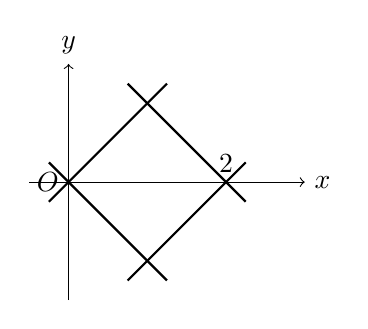
\begin{tikzpicture}[scale=1]
            \draw[->] (-0.5,0) -- (3,0) node[right] {$x$};
            \draw[->] (0,-1.5) -- (0,1.5) node[above] {$y$};

            \node at (0,0) [left] {$O$};
            \node at (2,0) [above] {2};

            \draw[domain=-0.25:1.25,samples=10,smooth,thick,black]
            plot (\x,\x);
            \draw[domain=-0.25:1.25,samples=10,smooth,thick,black]
            plot (\x,-\x);
            \draw[domain=0.75:2.25,samples=10,smooth,thick,black]
            plot (\x,2-\x);
            \draw[domain=0.75:2.25,samples=10,smooth,thick,black]
            plot (\x,\x-2);
            \end{tikzpicture}
        \end{center}
        由此,只需要考虑最大值$M$是出现在左侧还是右侧,即能找到符合要求的$\xi$。另一方面,由于上述图形的边界是\textbf{不可导}的($x=1$时),在$M\ne0$时不可能真正达到。接下来的证明即是以此为方向。

        \item \textbf{存在符合要求的$\xi$}

        由于$f(x)$是连续函数,$|f(x)|$也是连续函数,因此根据最值定理必然能取到最大值,设$c\in[0,2]$满足$|f(c)|=M$。若$M=0$,任取$\xi\in(0,2)$可发现结论已经成立,从而只需考虑$M>0$的情况,此时$c\in(0,2)$。    
        
        若$c\in(0,1]$,利用拉格朗日中值定理可知存在$\xi\in(0,c)$使得
        $$f'(\xi)=\frac{f(c)-f(0)}{c-0}=\frac{M}{c}\ge M$$
        若$c\in[1,2)$,利用拉格朗日中值定理可知存在$\xi\in(c,2)$使得
        $$f'(\xi)=\frac{f(2)-f(c)}{2-c}=-\frac{M}{2-c}\le -M$$
        无论哪种情况都存在符合要求的$\xi$。

        \item \textbf{证明$M=0$}
        
        反证,若$M>0$,我们接下来推出矛盾。在前一部分证明的基础上,若$c\in(0,1)$,找到的$f'(\xi)$已经满足$|f'(\xi)|=\frac{M}{c}>M$;若$c\in(1,2)$,找到的$f'(\xi)$已经满足$|f'(\xi)|=\frac{M}{2-c}>M$。由此,若$|f'(\xi)|$恒不超过$M$,只能$c=1$,即$|f(1)|=M$。我们不妨设$f(1)=M$,若$f(1)=-M$证明类似。

        由于$f'(x)$是连续函数,利用\textbf{微积分基本定理}可知
        $$M=f(1)=\int_0^1f'(x)\dr x$$
        两边同时用$M$减可得
        $$\int_0^1(M-f'(x))\dr x=0$$
        由于$f'(x)$为连续函数,且由条件$f'(x)\le M$,左侧非负,利用\exref{cont nonneg int}的结论(此结论可\textbf{直接使用})得必须
        $$\forall x\in[0,1],\quad M=f'(x)$$
        从而计算0到$x$的积分可得
        $$\forall x\in[0,1],\quad f(x)=Mx$$
        另一方面,再次利用微积分基本定理可得
        $$-M=f(2)-f(1)=\int_1^2f'(x)\dr x$$
        两边同时加$M$可得
        $$\int_1^2(M+f'(x))\dr x=0$$
        由于$f'(x)$为连续函数,且由条件$f'(x)\ge -M$,左侧非负,利用\exref{cont nonneg int}的结论得必须
        $$\forall x\in[1,2],\quad-M=f'(x)$$
        从而计算$x$到2的积分可得
        $$\forall x\in[1,2],\quad f(x)=M(2-x)$$
        这样,我们就得到了$f(x)$在$[0,2]$的完整表达式,但这样的$f$在1处左导数为$M$、右导数为$-M$,不相等,因此$f$在1处\textbf{不可导},矛盾。
    \end{itemize}
}
\end{framed}

\begin{framed}
\begin{exercise}
    对$[a,b]$上存二阶导数的函数$f(x)$,若已知$f(a)=f(b)=f'(a)=f'(b)=0$,且
    $$\forall x\in(a,b),\quad|f''(x)|\le M$$
    证明
    $$\forall x\in[a,b],\quad|f(x)|\le\frac{M}{16}(b-a)^2$$
\end{exercise}
\sol{
    \note 这题本质上\textbf{非常困难},对系数的改进很难通过简单的分析得到,由此几乎只能在大量的\textbf{几何观察}后逐步证明。 
    
    分为以下步骤:
    \begin{itemize}
        \item \textbf{初步分析}
        
        对任何$x\in(a,b)$,由本题的条件很容易想到直接在$a$、$b$进行带二阶拉格朗日余项的泰勒展开,从而得到存在$\theta_1\in(a,x)$、$\theta_2\in(x,b)$使得
        $$f(x)=\frac{(x-a)^2}{2}f''(\theta_1)$$
        $$f(x)=\frac{(b-x)^2}{2}f''(\theta_2)$$
        当$x\le\frac{a+b}{2}$时,从第一个式子可直接得出
        $$|f(x)|\le\frac{((a-b)/2)^2}{2}|f''(\theta_1)|\le\frac{M}{8}(b-a)^2$$
        当$x\ge\frac{a+b}{2}$时,同理从第二个式子可得出$|f(x)|\le\frac{(b-a)^2}{8}M$。由此,我们已经证明了
        $$|f(x)|\le\frac{M}{8}(b-a)^2$$
        但是,为了将$\frac{1}{8}$进一步压缩到$\frac{1}{16}$,我们必须开始思考$\frac{1}{8}$的界为何\textbf{事实上不可取等}。

        进一步研究可以发现,以取到$\frac{M}{8}(b-a)^2$的点为正为例,这意味着从$a$到$\frac{a+b}{2}$,$f(x)$几乎一直以\textbf{最大速度}增加,即$f(x)=\frac{M}{2}(x-a)^2$、$f'(x)=M(x-a)$。而从$\frac{a+b}{2}$,$f(x)$又需要以\textbf{最大速度}减小,即对应的$f(x)=\frac{M}{2}(b-x)^2$、$f'(x)=-M(b-x)$。然而,在$\frac{a+b}{2}$附近,$f'(x)$的值从$\frac{b-a}{2}M$\textbf{突变}到了$-\frac{b-a}{2}M$,这与它的斜率绝对值限制为$M$矛盾。

        \item \textbf{几何观察}
        
        由于如上的直接做法无法实现,我们需要重新考虑何时能让$|f(x)|$最大值尽可能大。由于此题同时涉及了一阶、二阶导函数,我们\textbf{以一阶导函数为中心}进行考虑。

        若画出$f'(x)$的图像,由$|f''(x)|\le M$可知它的\textbf{斜率}绝对值不超过$M$,且两端为0。另一方面,$f(a)=f(b)=0$又要求$f'(x)$在$x$轴\textbf{上下的面积}相同,这样才能得到整个区间上积分为0。要求的$|f(x)|$最大值即相当于$f'(x)$到某个位置的\textbf{有向面积最大值}。

        由此,一个自然的想法是,$f'(x)$最好情况应当是在$(a,\frac{a+b}{2})$为正、$(\frac{a+b}{2},b)$为负,这样即能保证$\frac{a+b}{2}$处尽量大。另一方面,又由于斜率的限制,$f'(x)$不能从0到$\frac{a+b}{2}$一直增加,因此最好情况应当\textbf{无限接近}下图:
        \begin{center}  
            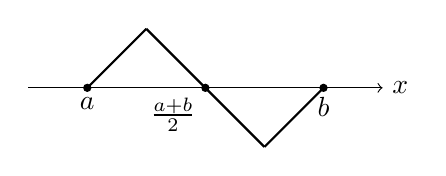
\begin{tikzpicture}[scale=1.5]
            \draw[->] (-0.5,0) -- (2.5,0) node[right] {$x$};
            \node at (0,0) [below] {$a$};
            \fill (0,0) circle(1pt);
            \node at (1,0) [below left] {$\frac{a+b}{2}$};
            \fill (1,0) circle(1pt);
            \node at (2,0) [below] {$b$};
            \fill (2,0) circle(1pt);

            \draw[domain=0:0.5,samples=10,smooth,thick,black]
            plot (\x,\x);
            \draw[domain=0.5:1.5,samples=10,smooth,thick,black]
            plot (\x,1-\x);
            \draw[domain=1.5:2,samples=10,smooth,thick,black]
            plot (\x,\x-2);
            \end{tikzpicture}
        \end{center}
        这里三段的斜率分别为$M$、$-M$、$M$,两次斜率转变点为$\frac{3a+b}{4}$与$\frac{3b+a}{4}$。对应的$f(x)$图像将接近三段\textbf{抛物线}的拼合:
        \begin{center}  
            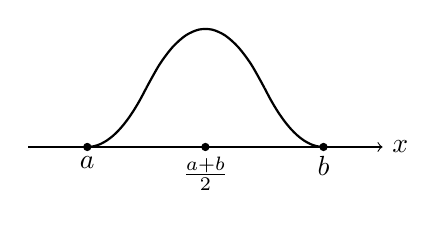
\begin{tikzpicture}[scale=1.5]
            \draw[->] (-0.5,0) -- (2.5,0) node[right] {$x$};
            \node at (0,0) [below] {$a$};
            \fill (0,0) circle(1pt);
            \node at (1,0) [below] {$\frac{a+b}{2}$};
            \fill (1,0) circle(1pt);
            \node at (2,0) [below] {$b$};
            \fill (2,0) circle(1pt);

            \draw[domain=0:0.5,samples=10,smooth,thick,black]
            plot (\x,{2*\x*\x});
            \draw[domain=0.5:1.5,samples=10,smooth,thick,black]
            plot (\x,{1-2*(\x-1)*(\x-1)});
            \draw[domain=1.5:2,samples=10,smooth,thick,black]
            plot (\x,{2*(\x-2)*(\x-2)});
            \end{tikzpicture}
        \end{center}

        有了这样的几何观察,我们即可以开始尝试证明。

        \item \textbf{导函数零点}
        
        从之前的几何讨论中可以发现,关键在于$f'(x)$在区间中的零点,零点前后$f'(x)$的值可以\textbf{通过斜率控制}。

        我们接下来只证明$f(x)$在$[a,b]$的\textbf{最大值}不超过$\frac{M}{16}(b-a)^2$,完全类似可证明最小值大于等于$-\frac{M}{16}(b-a)^2$。

        若$M=0$,由条件可发现$f(x)$在$[a,b]$恒为0,已经得证;在$M>0$时,若$f(x)$在$[a,b]$的最大值为0,也已经满足条件。下面假设$M>0$且$f(x)$在$[a,b]$的最大值大于0,则最大值点在$(a,b)$中,设$c\in(a,b)$为一个最大值点,且$f(c)=M_0$为最大值。

        由于区间内部的最大值点为极大值点,必然有$f'(c)=0$。接下来,我们只需要分别考虑左侧最高能升高到多少,右侧最多能降低多少,即能确定最大值。

        \item \textbf{进一步估算}
        
        类似前一题,我们将$[a,c]$\textbf{拆成两半}以保证$f'(x)$的大小可以得到控制。对$x\in(a,\frac{a+c}{2}]$,由拉格朗日中值定理可知存在$\xi\in(a,x)$使得
        $$\frac{f'(x)-f'(a)}{x-a}=f''(\xi)\le M$$
        也即
        $$f'(x)\le M(x-a)$$
        对$x\in[\frac{a+c}{2},a)$,由拉格朗日中值定理可知存在$\xi\in(x,c)$使得
        $$\frac{f'(c)-f'(x)}{c-x}=f''(\xi)\ge-M$$
        也即
        $$f'(x)\le M(c-x)$$
        综合以上,利用\textbf{微积分基本定理}(由$f''$存在,$f'$必然连续)可得
        $$\begin{aligned}f(c)&=\int_a^cf'(x)\dr x\\ &=\int_a^{(a+c)/2}f'(x)\dr x+\int_{(a+c)/2}^cf'(x)\dr x\\ &\le\int_a^{(a+c)/2}M(x-a)\dr x+\int_{(a+c)/2}^cM(c-x)\dr x\\ &=\frac{M}{4}(c-a)^2\end{aligned}$$
        同理,由拉格朗日中值定理可知$x\in(c,\frac{c+b}{2}]$时$f'(x)\ge -M(x-c)$、$x\in[\frac{c+b}{2},b)$时$f'(x)\ge -M(b-x)$,从而
        $$\begin{aligned}f(c)&=-\int_c^bf'(x)\dr x\\ &=-\int_c^{(c+b)/2}f'(x)\dr x-\int_{(c+b)/2}^bf'(x)\dr x\\ &\le\int_c^{(c+b)/2}M(x-c)\dr x+\int_{(c+b)/2}^bM(b-x)\dr x\\ &=\frac{M}{4}(b-c)^2\end{aligned}$$
        综合以上可得
        $$f(c)\le\min\bigg\{\frac{M}{4}(c-a)^2,\frac{M}{4}(b-c)^2\bigg\}$$
        $c\le\frac{a+b}{2}$时取第一项,否则取第二项,即得到
        $$f(c)\le\frac{M}{16}(b-a)^2$$
        从而得证。
    \end{itemize}
}
\end{framed}

\note 对于这类泰勒展开相关的估算问题,往往可以先确定条件从\textbf{几何}角度的理解,再尝试用代数描述几何。不过,具体的问题仍然可能非常具有技巧性。上面的例子均为从导函数性质确定原函数性质,从\textbf{原函数性质确定导函数性质}的一些例子可见本讲义12.3.3。

\subsection{多元函数}
\subsubsection{空间几何}
\note 空间几何相关的题目往往更接近\textbf{高中知识},但仍然需要大家掌握更\textbf{抽象}的向量代数描述。

\

\noindent\textbf{向量代数}

\begin{framed}
\begin{exercise}
    求曲线
    $$x=7t-14,\quad y=4t^2,\quad z=3t^3$$
    在参数$t=1$处对应的法平面方程。
\end{exercise}
\sol{
    直接计算可得
    $$(x'(t),y'(t),z'(t))=(7,8t,9t^2)$$
    从而它在$t=1$处的切向量为$(7,8,9)$。法平面指以曲线切向量为\textbf{法向量}且过对应点的平面。$t=1$对应$(-7,4,3)$,从而可写出平面的点法式
    $$7(x+7)+8(y-4)+9(z-3)=0$$
    从而化简得一般方程
    $$7x+8y+9z=10$$

    \note 本题是为了提醒大家\textbf{记忆基本概念},不要在考试时因为概念混淆而丢分。
}
\end{framed}

\begin{framed}
\begin{exercise}
    设$P_1$、$P_2$是三维空间单位球面$x^2+y^2+z^2=1$上的两个不同的点,$O$为坐标原点,计算
    $$|\overrightarrow{OP_1}\times\overrightarrow{OP_2}|^2+|\overrightarrow{OP_1}\cdot\overrightarrow{OP_2}|^2$$
\end{exercise}
\sol{
    由条件可知$|\overrightarrow{OP_1}|=|\overrightarrow{OP_2}|=1$。设$\overrightarrow{OP_1}$与$\overrightarrow{OP_2}$夹角为$\theta$\ ($\theta\in[0,\pi]$),利用定义可知
    $$|\overrightarrow{OP_1}\times\overrightarrow{OP_2}|=|\overrightarrow{OP_1}||\overrightarrow{OP_2}||\sin\theta|=\sin\theta$$
    $$\overrightarrow{OP_1}\cdot\overrightarrow{OP_2}=|\overrightarrow{OP_1}||\overrightarrow{OP_2}|\cos\theta=\cos\theta$$
    从而可直接得到结果为1。

    \note 虽然本题并不会用到,但仍然建议大家记忆\textbf{向量叉乘的坐标表示},更复杂的公式一般无需记忆。
}
\end{framed}

\begin{framed}
\begin{exercise}
    设异面直线$L_1$、$L_2$的方向向量为$\bm{r}_1$、$\bm{r}_2$,且已知$P_1\in L_1$、$P_2\in L_2$,用$\overrightarrow{P_1P_2}$、$\bm{r}_1$、$\bm{r}_2$表示$L_1$、$L_2$的距离。
\end{exercise}
\sol{
    从几何知识可以发现,若已知$L_1$、$L_2$的\textbf{公垂线},$\overrightarrow{P_1P_2}$到其的\textbf{投影长度}就应当是距离。利用定义,公垂线应当与$\bm{r}_1$、$\bm{r}_2$均垂直,从而由$\bm{r}_1$、$\bm{r}_2$不平行知它的方向向量可以为
    $$\bm{r}_1\times\bm{r}_2$$
    再利用内积的几何意义即得投影长度为
    $$\frac{|\overrightarrow{P_1P_2}\cdot(\bm{r}_1\times\bm{r}_2)|}{|\bm{r}_1\times\bm{r}_2|}$$

    \note 本题需要大家熟悉\textbf{点乘、叉乘与投影的几何意义},此外,异面直线的距离计算中,直接通过方程求解公垂线方向向量往往比计算叉乘更快。
}
\end{framed}

\note 投影的基本结论为,$\bm{a}$到非零向量$\bm{b}$的投影\textbf{长度}是$\frac{|\bm{a}\cdot\bm{b}|}{|\bm{b}|}$,投影\textbf{向量}是$\frac{\bm{a}\cdot\bm{b}}{|\bm{b}|}\bm{b}$。

\

\noindent\textbf{几何关系}

\begin{framed}
\begin{exercise}
    设$\rb^3$中平面$K$的方程为$x+3y+2z=6$,与$x$、$y$、$z$轴交点为$A$、$B$、$C$。求过原点与$A$、$B$、$C$的球面方程。
\end{exercise}
\sol{
    由与$x$轴交点仅有$x$分量非零,与$y$、$z$轴交点同理,直接代入计算可发现
    $$A(6,0,0),\quad B(0,2,0),\quad C(0,0,3)$$
    设球面方程为
    $$(x-a)^2+(y-b)^2+(z-c)^2=r^2$$
    可得
    $$\begin{cases}a^2+b^2+c^2=r^2\\(6-a)^2+b^2+c^2=r^2\\a^2+(2-b)^2+c^2=r^2\\a^2+b^2+(3-c)^2=r^2\end{cases}$$
    综合即解得球面方程为
    $$(x-3)^2+(y-1)^2+\bigg(z-\frac{3}{2}\bigg)^2=\frac{49}{4}$$
}
\end{framed}

\begin{framed}
\begin{exercise}
    设$\rb^3$中直线$L$为
    $$\begin{cases}2x+y-3z=0\\x+2y-z-2=0\end{cases}$$
    求其标准方程,并求与$L$相切的、以原点为中心的球面的方程,计算切点坐标。
\end{exercise}
\sol{
    利用线性代数知识,我们可以找到方程组的两个不同的解,对应直线上两点
    $$A(1,1,1),\quad B\bigg(-\frac{2}{3},\frac{4}{3},0\bigg)$$
    从而可得直线的一个方向向量为$\overrightarrow{AB}$,将其乘适当倍数得到更简单的形式$(-5,1,-3)$,由此得到直线的一个标准方程
    $$(x,y,z)=(1-5t,1+t,1-3t)$$
    设球面方程为
    $$x^2+y^2+z^2=r^2$$
    相切意味着
    $$(1-5t)^2+(1+t)^2+(1-3t)^2=r^2$$
    $3-14t+35t^2=r^2$
    只有唯一解,利用二次函数知识即得$r^2=\frac{8}{5}$,此时$t=\frac{1}{5}$,即切点$\big(0,\frac{6}{5},\frac{2}{5}\big)$。

    \note 可以证明,球面与直线或平面相切都\textbf{等价于交点唯一}。
}
\end{framed}

\begin{framed}
\begin{exercise}
    设$\rb^3$中平面$K$的方程为$x+3y+2z=6$,与$x$、$y$、$z$轴交点为$A$、$B$、$C$。$\rb^3$中的动点$H$与$K$距离为1,记$M$为$H$到$K$的投影,要求其在$\triangle ABC$内部,到三条边$BC$、$CA$、$AB$的距离为$p$、$q$、$r$。
    
    用$p$、$q$、$r$表示四面体$ABCH$的表面积$S(p,q,r)$,写出它们满足的约束条件,并以此计算$S(p,q,r)$在约束下的所有稳定点。
\end{exercise}
\sol{
    分为四部分计算:
    \begin{itemize}
        \item \textbf{三角形面积}
        
        由与$x$轴交点仅有$x$分量非零,与$y$、$z$轴交点同理,直接代入计算可发现
        $$A(6,0,0),\quad B(0,2,0),\quad C(0,0,3)$$
        利用叉乘的\textbf{几何意义},三角形$ABC$的面积应为
        $$\frac{1}{2}|\overrightarrow{AB}\times\overrightarrow{BC}|$$
        由此可直接算出其为$3\sqrt{14}$。

        \item \textbf{四面体表面积}
        
        由于$K$到$BC$的距离为$p$,$H$到平面$ABC$的距离为1,利用几何关系与勾股定理可知$H$到$BC$的距离为$\sqrt{p^2+1}$,又由$BC$长度为$\sqrt{13}$,即得三角形$HBC$面积为$\frac{\sqrt{13}}{2}\sqrt{p^2+1}$。同理可计算另外两个三角形面积,得到
        $$S(p,q,r)=3\sqrt{14}+\frac{\sqrt{13}}{2}\sqrt{p^2+1}+\sqrt{10}\sqrt{q^2+1}+\frac{3\sqrt5}{2}\sqrt{r^2+1}$$

        \item \textbf{约束条件}
        
        利用几何关系,连接$KA$、$KB$、$KC$,考虑分出的三个三角形面积可知
        $$\frac{1}{2}p|BC|+\frac{1}{2}q|CA|+\frac{1}{2}r|AB|=S_{\triangle ABC}$$
        从而代入可得约束
        $$\sqrt{13}p+2\sqrt{10}q+3\sqrt{5}r=6\sqrt{14}$$
        此外,三角形内部要求$p$、$q$、$r$均为\textbf{正实数}。

        \item \textbf{计算稳定点}
        
        构造辅助函数
        $$L(p,q,r,\lambda)=S(p,q,r)+\lambda(\sqrt{13}p+2\sqrt{10}q+3\sqrt{5}r-6\sqrt{14})$$
        对四个变量求导可得方程组
        $$\begin{cases}\frac{\sqrt{13}}{2}\frac{p}{\sqrt{1+p^2}}+\sqrt{13}\lambda=0\\\sqrt{10}\frac{q}{\sqrt{1+q^2}}+2\sqrt{10}\lambda=0\\\frac{3\sqrt{5}}{2}\frac{r}{\sqrt{1+r^2}}+3\sqrt{5}\lambda=0\\\sqrt{13}p+2\sqrt{10}q+3\sqrt{5}r=6\sqrt{14}\end{cases}$$
        从前三个方程可以化简得到
        $$\frac{p}{\sqrt{1+p^2}}=\frac{q}{\sqrt{1+q^2}}=\frac{r}{\sqrt{1+r^2}}$$
        求导可发现$\frac{t}{\sqrt{1+t^2}}$随$t$单调增,从而必须$p=q=r$,这就得到了唯一稳定点
        $$p=q=r=\frac{6\sqrt{14}}{\sqrt{13}+2\sqrt{10}+3\sqrt{5}}$$

        \note 这事实上是表面积的\textbf{最小值}点。
    \end{itemize}

    \note 对解析几何问题,寻找\textbf{合适的计算路径}可以有效降低计算量。
}
\end{framed}

\subsubsection{极限与可微性}
\noindent\textbf{极限计算}

\note 多元函数极限问题非常不建议使用泰勒展开等手段,除了\textbf{非常难以严谨}外,还因为展开为多项式后\textbf{多元多项式之比的极限}仍然很难确定。

\begin{framed}
\begin{exercise}
    判断以下极限是否存在,若存在,计算其值:
    $$\lim_{(x,y)\to(0,0)}(x^2+y^2)^{x^2}$$
\end{exercise}
\sol{
    设$f(x,y)=x^2\ln(x^2+y^2)$,考虑\textbf{极坐标}表示,在$r>0$时有
    $$f(r\cos\theta,r\sin\theta)=2\cos^2\theta r^2\ln r$$
    于是
    $$|f(r\cos\theta,r\sin\theta)|\le2|r^2\ln r|$$
    类似\exref{poly exp}中可证明(这可以\textbf{直接使用})
    $$\lim_{r\to 0^+}|r^2\ln r|=0$$
    从而由定义可发现$r=\sqrt{x^2+y^2}$时
    $$\lim_{(x,y)\to(0,0)}|r^2\ln r|=0$$
    再由\textbf{夹逼定理}($f(x,y)$在$-2|r^2\ln r|$与$2|r^2\ln r|$之间)即得到
    $$\lim_{(x,y)\to(0,0)}f(x,y)=0$$
    由于原极限为$\er^{f(x,y)}$的极限,且指数函数连续,由\textbf{复合函数极限结论}即得
    $$\lim_{(x,y)\to(0,0)}(x^2+y^2)^{x^2}=1$$

    \note 取\textbf{对数}与\textbf{极坐标}分析是多元函数极限的最基本做法。
}
\end{framed}

\begin{framed}
\begin{exercise}
    判断以下极限是否存在,若存在,计算其值:
    $$\lim_{(x,y)\to(0,0)}\frac{xy}{x^2+(\er^y-1)^2}$$
\end{exercise}
\sol{
    \note 采用阶估算的思路:由等价无穷小,分母近似为$x^2+y^2$,而$\frac{xy}{x^2+y^2}$沿不同方向趋于0时极限不同,可以\textbf{猜测}其极限不存在,并从\textbf{类似路径}证明。

    当沿着$y=0$的路径趋于0时,对应极限为
    $$\lim_{x\to0}\frac{x\cdot0}{x^2+0^2}=0$$
    当沿着$y=x$的路径趋于0时,对应极限为
    $$\lim_{x\to0}\frac{x^2}{x^2+(\er^x-1)^2}=\lim_{x\to0}\frac{1}{1+((\er^x-1)/x)^2}$$
    利用等价无穷小与乘除极限即得此极限为$\frac{1}{2}$,由于$\frac{1}{2}\ne0$,原极限不存在。
}
\end{framed}

\begin{framed}
\begin{exercise}
    判断以下极限是否存在,若存在,计算其值:
    $$\lim_{(x,y)\to(0,0)}\frac{xy(\er^y-1)}{x^2+y^2}$$
\end{exercise}
\sol{
    \note 注意这里\textbf{无法使用等价无穷小替换},因为$(x,y)\to(0,0)$时$\frac{\er^y-1}{y}$无法保证在0的去心邻域有定义,极限\textbf{不存在}。本讲义15.2对这类情况进行了一些讨论。

    \note 从直观来看,分子近似为$xy^2$,为三次,而分母为二次,分子次数更高,因此极限可能为0。为了进行更严谨的证明,我们仍然需要利用\textbf{极坐标}进行放缩。

    设$f(x,y)=\frac{xy(\er^y-1)}{x^2+y^2}$,考虑极坐标表示,在$r>0$时有
    $$f(r\cos\theta,r\sin\theta)=\cos\theta\sin\theta(\er^{r\cos\theta}-1)$$
    由于我们已知$t\to0$时$(\er^t-1)\sim t$,利用极限\textbf{保序性},存在$\delta_0>0$使得$0<|t|<\delta_0$时
    $$\bigg|\frac{\er^t-1}{t}\bigg|<2$$
    同乘$|t|$,并考虑$t=0$的情况可发现$|t|<\delta_0$时$|\er^t-1|\le2|t|$。由此,在$r\in(0,\delta_0)$时,利用$|r\cos\theta|<\delta_0$,必然有
    $$|f(r\cos\theta,r\sin\theta)|\le|\er^{r\cos\theta}-1|\le2|r\cos\theta|\le 2r$$
    由初等函数连续性
    $$\lim_{(x,y)\to(0,0)}2\sqrt{x^2+y^2}=0$$
    利用\textbf{夹逼定理}(在$r<\delta_0$时$f(x,y)$在$-2r$与$2r$之间)即得到
    $$\lim_{(x,y)\to(0,0)}f(x,y)=0$$
}
\end{framed}

\begin{framed}
\begin{exercise}
    判断以下极限是否存在,若存在,计算其值:
    $$\lim_{(x,y)\to(0,0)}\frac{24\cos\sqrt{x^2+y^2}-24+12(x^2+y^2)+3(x^5+y^5)}{\tan^4\sqrt{x^2+y^2}}$$
\end{exercise}
\sol{
    \note 观察可以发现,本题分为了与$x^2+y^2$有关、无关的两部分,由此想到\textbf{分别处理}。

    记
    $$f(t)=\frac{24\cos t-24+12t^2}{\tan^4t},\quad g(x,y)=\frac{x^5+y^5}{\tan^4\sqrt{x^2+y^2}}$$
    则原极限为
    $$\lim_{(x,y)\to(0,0)}\big(f(\sqrt{x^2+y^2})+3g(x,y)\big)$$
    我们下面分别计算:
    \begin{itemize}
        \item \textbf{$f$的极限}
        
        由余弦函数的泰勒展开结论知
        $$\cos t=1-\frac{1}{2}t^2+\frac{1}{24}t^4+o(t^4)\quad(t\to0)$$
        从而利用等价无穷小替换可知
        $$\lim_{t\to0}f(t)=\lim_{t\to0}\frac{24\cos t-24+12t^2}{t^4}=\lim_{t\to0}\frac{t^4+o(t^4)}{t^4}=1$$
        最后一步是利用了$o(t^4)$的定义。

        由于$(x,y)\to(0,0)$时$\sqrt{x^2+y^2}$极限为0,且在0的\textbf{去心邻域非零},由复合函数极限结论即得
        $$\lim_{(x,y)\to(0,0)}f(\sqrt{x^2+y^2})=\lim_{t\to0}f(t)=1$$

        \note 注意复合函数极限结论需要\textbf{验证条件}。

        \item \textbf{$g$的极限}
        
        由于分子次数更高,我们可以\textbf{猜测}其极限为0。利用极坐标表示,在$r>0$时有
        $$g(r\cos\theta,r\sin\theta)=\frac{r^5}{\tan^4r}(\cos^5\theta+\sin^5\theta)$$
        于是
        $$|g(r\cos\theta,r\sin\theta)|\le\bigg|\frac{2r^5}{\tan^4r}\bigg|$$
        直接由等价无穷小计算可知
        $$\lim_{r\to0^+}\frac{2r^5}{\tan^4r}=\lim_{r\to0^+}\frac{2r^5}{r^4}=0$$
        从而由定义可发现$r=\sqrt{x^2+y^2}$时
        $$\lim_{(x,y)\to(0,0)}\bigg|\frac{2r^5}{\tan^4r}\bigg|=0$$
        再由\textbf{夹逼定理}($g(x,y)$在$-\big|\frac{2r^5}{\tan^4r}\big|$与$\big|\frac{2r^5}{\tan^4r}\big|$之间)即得到
        $$\lim_{(x,y)\to(0,0)}g(x,y)=0$$
    \end{itemize}

    综合以上与极限的四则运算性质得到原极限为1。
}
\end{framed}

\note 可以\textbf{直接使用}如下结论(证明见\exref{2 dim polar}):在极坐标表示下,若存在$\delta>0$使得$r\in(0,\delta)$时$|f(x,y)|\le F(r)$,且
$$\lim_{r\to0^+}F(r)=0$$
则有
$$\lim_{(x,y)\to(0,0)}f(x,y)=0$$
上方的极限证明题均可以此简化说明。

\

\noindent\textbf{可微性定义}

\begin{framed}
\begin{exercise}
    设
    $$f(x,y)=\begin{cases}y\arctan\frac{1}{\sqrt{x^2+y^2}}&(x,y)\ne(0,0)\\0&(x,y)=(0,0)\end{cases}$$
    判断它在原点是否可微。
\end{exercise}
\sol{
    先计算\textbf{偏导数}。在直线$y=0$上,$f(x,y)$恒为0,从而其对$x$偏导为0,也即
    $$\partial_1f(0,0)=0$$
    在直线$x=0$上,有
    $$f(0,y)=\begin{cases}y\arctan\frac{1}{|y|}&y\ne0\\0&y=0\end{cases}$$
    从而$(0,0)$处其对$y$的偏导数为(这里第二个等号进行了换元$t=\frac{1}{|y|}$,它在$y\to0$时趋于正无穷)
    $$\lim_{y\to0}\frac{f(0,y)}{y}=\lim_{y\to0}\arctan\frac{1}{|y|}=\lim_{t\to+\infty}\arctan t=\frac{\pi}{2}$$
    若其可微,意味着
    $$f(x,y)-f(0,0)-x\partial_1f(0,0)-y\partial_2f(0,0)=o(\sqrt{x^2+y^2})\quad(x,y)\to(0,0)$$
    代入也即等价于
    $$g(x,y)=\frac{y\arctan\frac{1}{\sqrt{x^2+y^2}}-y\frac{\pi}{2}}{\sqrt{x^2+y^2}}$$
    在0处极限为0。
    
    利用极坐标表示,在$r>0$时有
    $$g(r\cos\theta,r\sin\theta)=\bigg(\arctan\frac{1}{r}-\frac{\pi}{2}\bigg)\sin\theta$$
    从而
    $$|g(r\cos\theta,r\sin\theta)|\le\bigg|\arctan\frac{1}{r}-\frac{\pi}{2}\bigg|$$
    通过$\arctan$的极限性质可知右侧在$r\to0^+$时的极限为0,由上方介绍的判别法即得左侧在原点极限为0,因此$f(x,y)$在原点\textbf{可微}。

    \note 由于偏导连续能推出可微,但可微无法推出偏导连续,对于一般的函数往往直接\textbf{利用定义}研究可微性更加方便。
}
\end{framed}

\begin{framed}
\begin{exercise}
    设$f(x,y)$在原点某邻域内有定义、在原点连续,且存在$A\in\rb$使得
    $$\lim_{(x,y)\to(0,0)}\frac{f(x,y)}{x^2+y^2}=A$$
    证明$f(x,y)$在原点可微。
\end{exercise}
\sol{
    利用乘积极限与\textbf{连续性}可知
    $$f(0,0)=\lim_{(x,y)\to(0,0)}f(x,y)=\lim_{(x,y)\to(0,0)}\frac{f(x,y)}{x^2+y^2}\cdot(x^2+y^2)=A\cdot0=0$$
    先计算\textbf{偏导数}。原点处$f$对第一个分量的偏导数由定义为
    $$\partial_1f(0,0)=\lim_{x\to0}\frac{f(x,0)}{x}$$
    在$f$满足的条件中考虑沿着$y=0$趋于0的情况可得
    $$\lim_{x\to0}\frac{f(x,0)}{x^2}=A$$
    于是
    $$\lim_{x\to0}\frac{f(x,0)}{x}=\lim_{x\to0}\frac{f(x,0)}{x^2}\cdot x=A\cdot0=0$$
    这就得到了$\partial_1f(0,0)=0$。同理,$\partial_2f(0,0)=0$。

    若其可微,意味着
    $$f(x,y)-f(0,0)-x\partial_1f(0,0)-y\partial_2f(0,0)=o(\sqrt{x^2+y^2})\quad(x,y)\to(0,0)$$
    由定义可将上式直接改写为
    $$\lim_{(x,y)\to(0,0)}\frac{f(x,y)}{\sqrt{x^2+y^2}}=0$$
    而这可以通过
    $$\lim_{(x,y)\to(0,0)}\frac{f(x,y)}{\sqrt{x^2+y^2}}=\lim_{(x,y)\to(0,0)}\frac{f(x,y)}{x^2+y^2}\cdot\sqrt{x^2+y^2}=A\cdot0=0$$
    得到,从而得证。
}
\end{framed}

\subsubsection{多元函数求导}
\noindent\textbf{偏导计算}

\begin{framed}
\begin{exercise}
    证明或否定:若$z$可以看成$x$与$y$的函数,也可以看成$a$与$b$的函数,且$x=a$,则必然有$z_x=z_a$。
\end{exercise}
\sol{
    考虑
    $$x=a,\quad y=a+b,\quad z=y=a+b$$
    则有
    $$z_x=0,\quad z_a=1$$
    从而答案是\textbf{否定}的。

    \note 这意味着计算偏导数必须\textbf{完全确定看作哪些变量的函数},不能只确定部分。
}
\end{framed}

\note 这部分的一些严谨性问题可参考本讲义第14章。

\begin{framed}
\begin{exercise}
    设函数$h(x,t)=f(x+at)+g(x-at)$,其中$f$、$g$在$\rb$上存在二阶导函数,$a\in\rb$为参数,计算$\partial_2^2h(x,t)-a^2\partial_1^2h(x,t)$。
\end{exercise}
\sol{
    直接利用复合函数求导公式计算
    $$\partial_1h(x,t)=\frac{\partial f(x+at)}{\partial x}+\frac{\partial g(x-at)}{\partial x}=f'(x+at)+g'(x-at)$$
    $$\partial_2h(x,t)=\frac{\partial f(x+at)}{\partial t}+\frac{\partial g(x-at)}{\partial t}=af'(x+at)-ag'(x-at)$$
    同理
    $$\partial_1^2h(x,t)=f''(x+at)+g''(x-at)$$
    $$\partial_2^2h(x,t)=a^2f''(x+at)+a^2g''(x-at)$$
    由此即得
    $$\partial_2^2h(x,t)-a^2\partial_1^2h(x,t)=0$$
}
\end{framed}

\begin{framed}
\begin{exercise}
    设函数
    $$T(x,y)=f(x)-f(y)-\sum_{k=1}^n\frac{f^{(k)}(y)}{k!}(x-y)^k$$
    其中$f$在$\rb$上存在$n+1$阶导函数,计算$\partial_2T(x,y)$。
\end{exercise}
\sol{
    直接计算可知所求目标为
    $$\frac{\partial T(x,y)}{\partial y}=-f'(y)-\sum_{k=1}^n\frac{\partial}{\partial y}\bigg(\frac{f^{(k)}(y)}{k!}(x-y)^k\bigg)$$
    利用乘积求导公式可发现(假设$0!=1$,则等号对$k=1$也成立)
    $$-\frac{\partial}{\partial y}\bigg(\frac{f^{(k)}(y)}{k!}(x-y)^k\bigg)=\frac{f^{(k)}(y)}{(k-1)!}(x-y)^{k-1}-\frac{f^{(k+1)}(y)}{k!}(x-y)^k$$
    可以发现,它对$k$求和时可以裂项相消,从而只剩下第一项与最后一项
    $$-\sum_{k=1}^n\frac{\partial}{\partial y}\bigg(\frac{f^{(k)}(y)}{k!}(x-y)^k\bigg)=f'(y)-\frac{f^{(n+1)}(y)}{n!}(x-y)^n$$
    由此即得最终结果为
    $$-\frac{f^{(n+1)}(y)}{n!}(x-y)^n$$
}
\end{framed}

\begin{framed}
\begin{exercise}
    已知
    $$x^2z_x+y^2z_y=z^2$$
    作代换
    $$x=t,\quad y=\frac{t}{1+tu},\quad z=\frac{t}{1+tW}$$
    将$W$看作$t$、$u$的函数$W=f(t,u)$,证明$\partial_1f(t,u)=0$。
\end{exercise}
\sol{
    我们提供两种思路:
    \begin{itemize}
        \item \textbf{条件出发}
        
        为了将\textbf{条件}转化为$t$、$u$、$W$的等式,一个核心思路是,$x$、$y$、$z$用$t$、$u$、$W$表示后,想化简$z_x$、$z_y$应当由换元后\textbf{对应}的一阶导数$W_t$、$W_u$表示。直接计算可得
        $$t=x,\quad u=\frac{1}{y}-\frac{1}{x},\quad W=\frac{1}{z}-\frac{1}{x}$$
        接下来需要化简$z_x$与$z_y$。将$t$、$u$、$W$\textbf{匹配}(也即将$z$看作$t$、$u$、$W$的函数)可得
        $$z_t=\frac{1}{(1+tW)^2},\quad z_u=0,\quad z_W=-\frac{t^2}{(1+tW)^2}$$
        从而直接计算导数,利用$t_x=1$有
        $$z_x=z_tt_x+z_uu_x+z_WW_x=\frac{1-t^2W_x}{(1+tW)^2}$$
        此处,若我们计算$W_x$时再将$W$看作$x$、$y$的函数,最终只能得到$z_x=z_x$,\textbf{没有更多有效信息}。但根据条件,我们将$W$看作$f(t,u)$,并\textbf{匹配}$t$、$u$即能得到(注意$W_t$代表将$u$看作常数,与$z_t$代表将$u$、$W$看作常数含义\textbf{不同})
        $$W_x=W_tt_x+W_uu_x=W_t+\frac{1}{x^2}W_u$$
        综合即得(事实上\textbf{直接}将$z$看作$t$、$u$的函数,$W$写为$f(t,u)$可得相同结果)
        $$z_x=\frac{1-t^2W_t-W_u}{(1+tW)^2},\quad x^2z_x=\frac{t^2-t^4W_t-t^2W_u}{(1+tW)^2}$$
        同理有(这里暂时不将$y$代入,方便之后计算)
        $$z_y=z_tt_y+z_uu_y+z_WW_y=-\frac{t^2W_y}{(1+tW)^2}$$
        $$W_y=W_tt_y+W_uu_y=-\frac{W_u}{y^2}$$
        综合并代入可得
        $$z_y=\frac{t^2W_u}{y^2(1+tW)^2},\quad y^2z_y=\frac{t^2W_u}{(1+tW)^2}$$
        由此,代入可发现条件最终化为了
        $$\frac{t^2-t^4W_t-t^2W_u}{(1+tW)^2}+\frac{t^2W_u}{(1+tW)^2}=\frac{t^2}{(1+tW)^2}$$
        从而化简即得到(由代换可进行,分母不会为0)
        $$\frac{t^4W_t}{(1+tW)^2}=0$$
        当$t=0$时,$u$、$W$任取对$y$、$z$无影响,于是$W$\textbf{无法看作}$t$、$u$的函数。其他情况下即得到$W_t=0$,这就完成了证明。

        \item \textbf{结论出发}
        
        设$z=g(x,y)$,则条件即关于$g$的条件
        $$x^2\partial_1g(x,y)+y^2\partial_2g(x,y)=g^2(x,y)$$
        由于$t$、$u$只与$x$、$y$有关,这其实是一个\textbf{显函数}问题,而非隐函数,直接求解可知
        $$W=\frac{1}{z}-\frac{1}{x}=\frac{1}{g(x,y)}-\frac{1}{x}=\frac{1}{g\big(t,\frac{t}{1+tu}\big)}-\frac{1}{t}$$
        从而将$t$、$u$匹配,直接计算有
        $$\frac{\partial W}{\partial t}=-\frac{1}{g^2\big(t,\frac{t}{1+tu}\big)}\frac{\partial g\big(t,\frac{t}{1+tu}\big)}{\partial t}+\frac{1}{t^2}=-\frac{\partial_1g\big(t,\frac{t}{1+tu}\big)+\frac{1}{(1+tu)^2}\partial_2g\big(t,\frac{t}{1+tu}\big)}{g^2\big(t,\frac{t}{1+tu}\big)}+\frac{1}{t^2}$$
        通分即得
        $$\frac{\partial W}{\partial t}=\frac{g^2\big(t,\frac{t}{1+tu}\big)-t^2\partial_1g\big(t,\frac{t}{1+tu}\big)-\frac{t^2}{(1+tu)^2}\partial_2g\big(t,\frac{t}{1+tu}\big)}{t^2g^2\big(t,\frac{t}{1+tu}\big)}$$
        注意由换元过程,分母即为条件中的$z^2-x^2z_x-y^2z_y$,由此在导函数有意义的点必有$W_t=0$,从而得证。
    \end{itemize}
}
\end{framed}

\note 从\textbf{条件}或\textbf{结论}开始\textbf{逐步转化向目标}进行计算是证明微分等式的常用方法。

\

\noindent\textbf{隐函数与反函数}

\note 这部分的题目需要在\textbf{细心计算}的基础上结合实际形式进行代数处理与化简,虽然总体较为灵活,但基本都可以\textbf{硬算}得到结果。仍然注意偏导数相关的严谨性。

\begin{framed}
\begin{exercise}
    求$\rb^2$中曲线
    $$x^2(y+1)^2+\int_0^{xy}\frac{\dr t}{\sqrt{t^3+1}}=1$$
    在$(1,0)$处的切线方程。
\end{exercise}
\sol{
    将$y$看作隐函数$y=f(x)$,方程对$x$求导得到(利用变上限积分的导数结论与复合函数求导)
    $$2x(y+1)^2+2x^2(y+1)f'(x)+\frac{1}{\sqrt{x^3y^3+1}}\frac{\dr(xy)}{\dr x}=0$$
    也即
    $$2x(y+1)^2+2x^2(y+1)f'(x)+\frac{1}{\sqrt{x^3y^3+1}}(y+xf'(x))=0$$
    代入$x=1$、$y=0$即解得
    $$f'(1)=-\frac{2}{3}$$
    从而切线方程即为
    $$y=-\frac{2}{3}(x-1)$$
}
\end{framed}

\begin{framed}
\begin{exercise}
    证明对任何$k\in\rb$,存在$(1,1)$的邻域$U$使得方程
    $$x^k-3x^2y+3xy^2-y^k=0$$
    在$U$中确定唯一的隐函数$y=f(x)$,且$f(1)=1$。
\end{exercise}
\sol{
    首先,无论$k$是多少,$(x,y)=(1,1)$均满足方程。考虑$y=f(x)$,方程两边同时对$x$求导得到
    $$kx^{k-1}-6xy-3x^2f'(x)+3y^2+6xyf'(x)-ky^{k-1}f'(x)=0$$
    代入$x=y=1$得到
    $$(k-3)f'(1)=k-3$$
    当$k\ne3$时,直接由\textbf{隐函数定理}可知邻域中存在唯一的隐函数$y=f(x)$满足条件。

    $k=3$时,可发现方程可化为$(x-y)^3=0$,由$x$、$y$为实数可直接解出$y=x$,从而\textbf{也确定了}唯一的隐函数$y=x$。

    \note 由此可见,隐函数定理只保证了确定隐函数的\textbf{充分性},即使无法使用隐函数定理,仍然可能确定唯一的隐函数。
}
\end{framed}

\begin{framed}
\begin{exercise}
    给定方程组
    $$\begin{cases}xy+yz^2+4=0\\x^2y+yz-z^2+5=0\end{cases}$$
    判断它在$(1,-2,1)$附近能确定的所有可能的隐函数,并计算导数。
\end{exercise}
\sol{
    代入可直接验证$(1,-2,1)$满足两个方程。由于此方程组包含两个方程,对应两个因变量,从而存在三种可能,接下来一一判别:
    \begin{itemize}
        \item \textbf{$y$、$z$看作$x$的函数}
        
        将$y$、$z$看作$x$的函数后,两方程对$x$求导得到
        $$\begin{cases}y+xy_x+y_xz^2+2yzz_x=0\\2xy+x^2y_x+y_xz+yz_x-2zz_x=0\end{cases}$$
        代入$(1,-2,1)$可得
        $$\begin{cases}-2+2y_x-4z_x=0\\-4+2y_x-4z_x=0\end{cases}$$
        此方程组\textbf{无解},从而无法将$y$、$z$看作$x$的函数。
        
        \item \textbf{$x$、$z$看作$y$的函数}
        
        将$x$、$z$看作$y$的函数后,与上方类似,两方程对$y$求导并代入$(1,-2,1)$可得
        $$\begin{cases}-2x_y+2-4z_y=0\\-4x_y+2-4z_y=0\end{cases}$$
        此方程组存唯一解$x_y=0$、$z_y=\frac{1}{2}$,从而可以确定$x$、$z$看作$y$的函数,导数如上。
        
        \item \textbf{$x$、$y$看作$z$的函数}
        
        将$x$、$y$看作$z$的函数后,与上方类似,两方程对$y$求导并代入$(1,-2,1)$可得
        $$\begin{cases}-2x_z+2y_z-4=0\\-4x_z+2y_z-4=0\end{cases}$$
        此方程组存唯一解$x_z=0$、$y_z=2$,从而可以确定$x$、$y$看作$z$的函数,导数如上。
    \end{itemize}

    \note 隐函数定理可以表述为,求导后得到的方程组\textbf{存唯一解}时,必然能找到对应的隐函数。这样就无需背诵利用Jacobi行列式的形式。
    
    如果背诵了隐函数定理,本题有\textbf{更简单的判定方法}:设两个方程为$F(x,y,z)=0$、$G(x,y,z)=0$,则有
    $$\partial_1F(x,y,z)=y,\quad\partial_2F(x,y,z)=x+z^2,\quad\partial_3F(x,y,z)=2yz$$
    $$\partial_1G(x,y,z)=2xy,\quad\partial_2G(x,y,z)=x^2+z,\quad\partial_3G(x,y,z)=y-2z$$
    由此可知
    $$\partial_1F(1,-2,1)=-2,\quad\partial_2F(1,-2,1)=2,\quad\partial_3F(1,-2,1)=-4$$
    $$\partial_1G(1,-2,1)=-4,\quad\partial_2G(1,-2,1)=2,\quad\partial_3G(1,-2,1)=-4$$
    进一步计算得
    $$\frac{D(F(x,y,z),G(x,y,z))}{D(y,z)}=0$$
    $$\frac{D(F(x,y,z),G(x,y,z))}{D(z,x)}=8\ne0$$
    $$\frac{D(F(x,y,z),G(x,y,z))}{D(x,y)}=4\ne0$$
    从而$x$、$z$可看作$y$的函数,$x$、$y$可看作$z$的函数,但$y$、$z$不能看作$x$的函数。虽然计算偏导数仍然需要按上述方法进行,但提前计算$F$、$G$的各偏导数可以通过复合函数导数结论\textbf{大幅简化}之后的计算。例如,将$x$、$z$看作$y$的函数时有
    $$\frac{\dr F(x,y,z)}{\dr y}=\partial_1F(x,y,z)x_y+\partial_2F(x,y,z)+\partial_3F(x,y,z)z_y$$

    \note 注意实际上不满足隐函数定理无法\textbf{直接确定不为隐函数},但剩下的细节过于复杂,考试一般不作要求。
}
\end{framed}

\begin{framed}
\begin{exercise}
    设$\rb^2$上的函数
    $$f(x,y)=x^2+2xy\sin(x+y)-y^2$$
    证明存在原点的邻域$D$与$D$上连续可微的\textbf{可逆}变换$x=g(u,v)$、$y=h(u,v)$,使得$g(0,0)=h(0,0)=0$,且
    $$f(g(u,v),h(u,v))=u^2-v^2$$
\end{exercise}
\sol{
    \note 本题的关键在于,换元$x=g(u,v)$、$y=h(u,v)$后,可得到\textbf{等式}
    $$x^2+2xy\sin(x+y)-y^2=u^2-v^2$$
    但是,尝试可发现,直接构造$g$、$h$是非常困难的。联系条件中的可逆,我们想到,先构造$u=g_0(x,y)$、$v=h_0(x,y)$\ (通过配方,这是更加简单的),再通过\textbf{反函数定理}找到$x$、$y$。

    直接配方可发现
    $$\begin{aligned}x^2+2xy\sin(x+y)-y^2&=(x+y\sin(x+y))^2-y^2-\sin^2(x+y)y^2\\ &=(x+y\sin(x+y))^2-\left(y\sqrt{1+\sin^2(x+y)}\right)^2\end{aligned}$$
    由此,我们取
    $$u=g_0(x,y)=x+y\sin(x+y)$$
    $$v=h_0(x,y)=y\sqrt{1+\sin^2(x+y)}$$
    当$x=y=0$时,的确可以得到$u$、$v$均为0,且直接计算可知
    $$u_x=1+y\cos(x+y),\quad u_y=\sin(x+y)+y\cos(x+y)$$
    $$v_x=\frac{y\sin(x+y)\cos(x+y)}{\sqrt{1+\sin^2(x+y)}},\quad v_y=\sqrt{1+\sin^2(x+y)}+\frac{y\sin(x+y)\cos(x+y)}{\sqrt{1+\sin^2(x+y)}}$$
    由此在$(0,0)$处$u_x=1$、$u_y=0$、$v_x=0$、$v_y=1$,即得到$(0,0)$处的Jacobi行列式
    $$\frac{D(u,v)}{D(x,y)}\bigg|_{(0,0)}=(u_xv_y-v_xu_y)\big|_{(0,0)}=1\ne0$$
    于是根据反函数定理,局部存在$u=g_0(x,y)$、$v=h_0(x,y)$的\textbf{逆变换}$x=g(u,v)$、$y=h(u,v)$符合要求。
}
\end{framed}

\subsubsection{多元微分应用}
\noindent\textbf{中值与泰勒展开}

\begin{framed}
\begin{exercise}
    求$f(x,y)=x^{\sqrt{y}}$在$(1,1)$处的二阶泰勒多项式。
\end{exercise}
\sol{
    计算可得$f(1,1)=1$,且直接求导可知
    $$\partial_1f(x,y)=\sqrt{y}x^{\sqrt{y}-1},\quad\partial_1f(1,1)=1$$
    $$\partial_2f(x,y)=x^{\sqrt{y}}\ln x\cdot\frac{1}{2\sqrt{y}},\quad\partial_2f(1,1)=0$$
    $$\partial_1^2f(x,y)=\sqrt{y}(\sqrt{y}-1)x^{\sqrt{y}-2},\quad\partial_1^2f(1,1)=0$$
    $$\partial_2^2f(x,y)=x^{\sqrt{y}}\ln^2x\cdot\frac{1}{4y}-x^{\sqrt{y}}\ln x\cdot\frac{1}{4}y^{-3/2},\quad\partial_2^2f(1,1)=0$$
    $$\partial_1\partial_2f(x,y)=\partial_2\partial_1f(x,y)=\frac{1}{2\sqrt{y}}x^{\sqrt{y}-1}+\sqrt{y}x^{\sqrt{y}-1}\ln x\cdot\frac{1}{2\sqrt{y}},\quad\partial_1\partial_2f(1,1)=\partial_2\partial_1f(1,1)=\frac{1}{2}$$
    由此即得所求的二阶泰勒多项式为
    $$1+(x-1)+\frac{1}{2}(x-1)(y-1)$$
    
    \note 注意多元函数泰勒展开务必\textbf{尽量使用求导},少使用复合函数等方法,以避免阶估算等过程出错。对本题来说,看作$\er^{\sqrt{y}\ln x}$再进行计算可以有效\textbf{减少计算导数过程的错误}。
}
\end{framed}

\begin{framed}
\begin{exercise}
    设函数$f(u,v)$在$\rb^2$上有连续的各偏导数,且满足
    $$\forall x\in\rb,\quad f(x,1-x)=1$$
    证明方程组
    $$\begin{cases}u^2+v^2=1\\v\partial_1f(u,v)=u\partial_2f(u,v)\end{cases}$$
    至少有两个不同的解。
\end{exercise}
\sol{
    由方程组形式可以想到\textbf{极坐标}:设
    $$u=r\cos\theta,\quad v=r\sin\theta$$
    则第一个方程变为$r=1$,进一步计算有(直接计算可知$u_\theta=-v$、$v_\theta=u$)
    $$\frac{\partial f(u,v)}{\partial\theta}=\partial_1f(u,v)\frac{\partial u}{\partial\theta}+\partial_2f(u,v)\frac{\partial v}{\partial\theta}=-v\partial_1f(u,v)+u\partial_2f(u,v)$$
    从而第二个方程即化为$\frac{\partial f(u,v)}{\partial\theta}=0$。

    将第一个方程代入第二个方程(由于这时$r$已经消去,剩下的部分只与$\theta$相关,不再是偏导数),我们最终将两个方程合并为
    $$\begin{cases}r=1\\\frac{\dr f(\cos\theta,\sin\theta)}{\dr\theta}=0\end{cases}$$
    记$g(\theta)=f(\cos\theta,\sin\theta)$,可以发现,$[0,2\pi)$中每个满足$g'(\xi)=0$的$\xi$,都对应一个不同的解
    $$(u,v)=(\cos\xi,\sin\xi)$$
    由此,我们需要证明$[0,2\pi)$中至少有两个不同的$\xi$满足$g'(\xi)=0$。

    由条件$f(x,1-x)=1$,可发现$f(0,1)=f(1,0)=1$,也即
    $$g\bigg(\frac{\pi}{2}\bigg)=g(0)=1$$
    利用\textbf{罗尔中值定理}可知存在$\xi_1\in(0,\frac{\pi}{2})$使得$g'(\xi_1)=0$。

    进一步地,利用$g$的周期性可发现$g(2\pi)=g(0)=1$,再次利用罗尔中值定理可知存在$\xi_2\in(\frac{\pi}{2},2\pi)$使得$g'(\xi_2)=0$。这就已经找到了符合要求的两个解
    $$(\cos\xi_1,\sin\xi_1),\quad(\cos\xi_2,\sin\xi_2)$$
}
\end{framed}

\note 建议\textbf{熟悉}对$r$、$\theta$求导在直角坐标下的形式,即若$z=f(x,y)$,$f$可微,且$x=r\cos\theta$、$y=r\sin\theta$,将$z$分别看作$x$、$y$与$r$、$\theta$的函数,有
$$rz_r=xz_x+yz_y,\quad z_\theta=xz_y-yz_x$$

\

\noindent\textbf{方向导数与极值}

\begin{framed}
\begin{exercise}
    对函数
    $$f(x,y)=\begin{cases}\frac{2xy^3}{x^2+y^4}&(x,y)\ne(0,0)\\0&(x,y)=(0,0)\end{cases}$$
    计算原点处的方向导数
    $$\frac{\partial f}{\partial\bm{l}}\bigg|_{(0,0)}$$
    这里$\bm{l}=(\cos\alpha,\sin\alpha)$为某单位向量。
\end{exercise}
\sol{
    利用定义可知
    $$\frac{\partial f}{\partial\bm{l}}\bigg|_{(0,0)}=\lim_{r\to0}\frac{f(r\cos\alpha,r\sin\alpha)-f(0,0)}{r}=\lim_{r\to0}\frac{2r\cos\alpha\sin^3\alpha}{\cos^2\alpha+r^2\sin^4\alpha}$$
    由此,若$\cos\alpha=0$,可得上式恒为0,因此极限为0,否则由分子极限为0、分母极限非零可知极限为0,因此对任何$\alpha$均有
    $$\frac{\partial f}{\partial\bm{l}}\bigg|_{(0,0)}=0$$

    \note 注意由于未证明$f(x,y)$在原点可微,\textbf{无法直接通过偏导组合得到},必须\textbf{由定义计算}。
}
\end{framed}

\begin{framed}
\begin{exercise}
    若$g(x,y)$在$(x_0,y_0)$取到极小值,对$\alpha\in\rb$,$t=0$是否一定是$h(t)=g(x_0+t\cos\alpha,y_0+t\sin\alpha)$的极小值点?若对任何$\alpha\in\rb$,$t=0$都是$h(t)=g(x_0+t\cos\alpha,y_0+t\sin\alpha)$的极小值点,$g(x,y)$是否一定在$(x_0,y_0)$取到极小值?
\end{exercise}
\sol{
    分别说明:
    \begin{itemize}
        \item \textbf{多元极值推方向极值}
        
        结论是\textbf{正确}的。根据定义可知,若$g(x,y)$在$(x_0,y_0)$取极小值,存在$\delta>0$使得
        $$\forall \sqrt{(x-x_0)^2+(y-y_0)^2}<\delta,\quad g(x,y)\ge g(x_0,y_0)$$
        从而代入可得
        $$\forall|t|<\delta,\quad g(x_0+t\cos\alpha,y_0+t\sin\alpha)\ge g(x_0,y_0)$$
        这就说明了0是$h(t)$的极小值点。
        
        \item \textbf{方向极值推多元极值}
        
        结论是\textbf{错误}的。我们构造如下的反例:
        $$f(x,y)=\begin{cases}-1&y=x^2,\quad x\ne0\\0&y\ne x^2\ \text{or}\ (x,y)=(0,0)\end{cases}$$

        考虑原点处,对任何$\alpha\in\rb$,有
        $$h(t)=f(t\cos\alpha,t\sin\alpha)$$
        分类讨论:若$\cos\alpha=0$,对应$h(t)=f(0,t)=0$,因此$t=0$是$h(t)$的极小值点;若$\cos\alpha\ne0$,可发现$h(t_0)=-1$当且仅当$t_0\ne0$且
        $$t_0\sin\alpha=t_0^2\cos^2\alpha$$
        也即
        $$t_0=\frac{\sin\alpha}{\cos^2\alpha}$$
        由此,$h(t)$在$(-|t_0|,|t_0|)$中恒为0,$t=0$为其极小值点。

        但是,在原点的任何邻域中都存在$y=x^2$且$x\ne0$的点,设其为$(x_0,x_0^2)$,则
        $$0=f(0,0)>f(x_0,x_0^2)=-1$$
        从而原点不为$f(x,y)$的极小值点。

        \note 此函数是一个重要的反例,因为它在原点处的\textbf{所有方向导数存在且相等},但\textbf{不连续}。
    \end{itemize}
}
\end{framed}

\begin{framed}
\begin{exercise}
    设$z=f(x,y)$是由方程$z^3+xz-2y=0$确定的隐函数,求$f(x,y)$在$(1,1)$处方向导数最大值。
\end{exercise}
\sol{
    将$z$看作$f(x,y)$,方程两侧对$x$、$y$求偏导可知
    $$3z^2z_x+z+xz_x=0,\quad 3z^2z_y+xz_y-2=0$$
    从而
    $$z_x=-\frac{z}{3z^2+x},\quad z_y=\frac{2}{3z^2+x}$$
    代入$x=y=1$可得$z^3-z-2=0$,将其因式分解为$(z-1)(z^2+z+2)=0$,即得实数解仅有$z=1$,由此可知
    $$\partial_1f(1,1)=z_x|_{(1,1)}=-\frac{1}{4},\quad\partial_2f(1,1)=z_y|_{(1,1)}=\frac{1}{2}$$
    
    由$z_x$、$z_y$形式可知$f$的两个一阶偏导数都在$(1,1)$处\textbf{连续},从而利用方向导数结论可知在\textbf{梯度方向}达到方向导数最大值,最大值为
    $$\sqrt{(\partial_1f(1,1))^2+(\partial_2f(1,1))^2}=\frac{\sqrt5}{4}$$

    \note 注意方向导数结论的使用条件是有\textbf{连续}的一阶偏导数,此时方向导数在梯度$\bm{g}$方向取最大值$|\bm{g}|$,负梯度$-\bm{g}$方向取最小值$-|\bm{g}|$。
}
\end{framed}

\begin{framed}
\begin{exercise}
    设$f(x,y,z)=\big(\frac{2x}{z}\big)^y$,求其在$(\frac{1}{2},1,1)$处下降最快方向的单位向量。
\end{exercise}
\sol{
    直接计算可知
    $$\partial_1f(x,y,z)=\frac{2^y}{z^y}yx^{y-1},\quad,\partial_3f(x,y,z)=\bigg(\frac{2x}{z}\bigg)^y\ln\frac{2x}{z}\quad\partial_2f(x,y,z)=(2x)^y(-y)z^{-y-1}$$
    由此代入即得到$(\frac{1}{2},1,1)$处$f(x,y,z)$的梯度为$(2,0,-1)$。

    由于\textbf{下降最快}的方向即\textbf{方向导数最小}的方向,由$f$各偏导在$(\frac{1}{2},1,1)$的\textbf{连续性}知其为负梯度方向$(-2,0,1)$,对应的单位向量即负梯度除以模长得到的
    $$\frac{1}{\sqrt5}(-2,0,1)$$
}
\end{framed}

\begin{framed}
\begin{exercise}
    设$z=f(x,y)$是由方程$(x^2+y^2)z+\ln z+2(x+y+1)=0$确定的隐函数,求其所有可能极值点。
\end{exercise}
\sol{
    由方程形式可知$z>0$。将$z$看作$f(x,y)$,方程两侧对$x$、$y$求偏导可知
    $$(x^2+y^2)z_x+2xz+\frac{z_x}{z}+2=0,\quad (x^2+y^2)z_y+2yz+\frac{z_y}{z}+2=0$$
    从而
    $$z_x=-\frac{2(1+xz)}{x^2+y^2+\frac{1}{z}},\quad z_y=-\frac{2(1+yz)}{x^2+y^2+\frac{1}{z}}$$
    由于分母不会为0,在方程的任何解附近均可\textbf{唯一确定}隐函数。

    由于可导的隐函数极值点必然为\textbf{稳定点},有$z_x=z_y=0$,由$z\ne0$进一步解得
    $$x=y=-\frac{1}{z}$$
    代入方程得到
    $$\frac{2}{z}+\ln z-\frac{4}{z}+2=0$$
    由此
    $$\ln z+2=\frac{2}{z}$$
    由于左侧单调增、右侧单调减,有\textbf{唯一解}$z=1$,此时$x=y=-1$。

    接下来判断其是否为极值点。这里我们可以用更简单的方式计算二阶导数:由于
    $$z_{xx}=-2\frac{1}{x^2+y^2+\frac{1}{z}}\frac{\partial(1+xz)}{\partial x}-2(1+xz)\frac{\partial}{\partial x}\frac{1}{x^2+y^2+\frac{1}{z}}$$
    第二项在$1+xz=0$时一定为0,从而有
    $$z_{xx}|_{(-1,-1)}=-2\frac{1}{x^2+y^2+\frac{1}{z}}(z+xz_x)\bigg|_{(-1,-1)}=-\frac{2}{3}$$
    同理可知
    $$z_{yy}|_{(-1,-1)}=-2\frac{1}{x^2+y^2+\frac{1}{z}}(z+yz_y)\bigg|_{(-1,-1)}=-\frac{2}{3}$$
    $$z_{xy}|_{(-1,-1)}=-2\frac{1}{x^2+y^2+\frac{1}{z}}xz_y\bigg|_{(-1,-1)}=0$$
    由此可发现$A<0$、$B^2-AC<0$,为\textbf{极大值}点,极大值为1。

}
\end{framed}

\note 确定极值常需要在一阶导为0的点计算二阶导,此时注意\textbf{一阶导为0很可能可以简化二阶导计算}。

\

\noindent\textbf{最值问题}

\note 最值问题的基本做法是将\textbf{内部}与\textbf{边界处}分别考虑,接下来我们会用逐渐复杂的几个例子说明。

\begin{framed}
\begin{exercise}
    设参数$p>4$,求
    $$f(x)=(x^4)^{1/p}+(1-x^4)^{1/p}$$
    在$[-1,1]$上的最小值与全部最小值点。
\end{exercise}
\sol{
    我们先进行基本的化简:令$t=x^4$,则$t\in[0,1]$,只需要研究
    $$g(t)=t^{1/p}+(1-t)^{1/p}$$
    在区间$[0,1]$上的最小值,再对应还原回$x$即可。

    \note 本题若不进行这样的化简,在0处将\textbf{不可导},导致讨论更加复杂(最值点\textbf{可能出现在不可导点},需要单独讨论)。

    直接求导可知$t\in(0,1)$时
    $$g'(t)=\frac{1}{p}t^{1/p-1}-\frac{1}{p}(1-t)^{1/p-1}$$
    若在$t_0\in(0,1)$取到最小值,其必然为极小值,从而
    $$\frac{1}{p}t_0^{1/p-1}-\frac{1}{p}(1-t_0)^{1/p-1}=0$$
    由$t_0<1$、$1-t_0>0$,且$\frac{1}{p}-1<0$,移项并同时开方得到
    $$t_0=1-t_0$$
    由此$t_0=\frac{1}{2}$。直接计算有
    $$g(0)=g(1)=1,\quad g\bigg(\frac{1}{2}\bigg)=2^{1-1/p}>1$$
    从而最小值只能在$t=0$或$t=1$取到,对应$x=0$或$\pm1$,最小值为1。
}
\end{framed}

\note 注意最值点只能在\textbf{内部稳定点}、\textbf{边界}(即使边界可导且导函数非零也仍可能,如考虑$f(x)=x$在$[0,1]$的最值)或\textbf{不可导点}达到。

\begin{framed}
\begin{exercise}
    设$\rb^3$中平面$x+y+z=1$与圆柱面$x^2+y^2=1$交集为椭圆$R$,求$R$上与原点最近、最远的点。
\end{exercise}
\sol{
    由条件可知,设$f(x,y,z)=x^2+y^2+z^2$,问题变为在约束$x+y+z=1$、$x^2+y^2=1$时$f(x,y,z)$的最值,利用约束可将条件\textbf{简化}为
    $$f(x,y,z)=1+z^2$$
    构造辅助函数
    $$F(x,y,z,\lambda,\mu)=1+z^2+\lambda(x+y+z-1)+\mu(x^2+y^2-1)$$
    对五个变量求导可得到方程组
    $$\begin{cases}\lambda+2x\mu=0\\\lambda+2y\mu=0\\2z+\lambda=0\\x+y+z=1\\x^2+y^2=1\end{cases}$$
    比较前两个方程可发现$\mu=0$或$x=y$,若$\mu=0$,代入可发现$\lambda=0$,从而$z=0$,得到两组解
    $$(x,y,z)=(1,0,0),\quad(x,y,z)=(0,1,0)$$
    若$x=y$,代入可得到两组解
    $$(x,y,z)=\bigg(\frac{1}{\sqrt2},\frac{1}{\sqrt2},1-\sqrt2\bigg),\quad(x,y,z)=\bigg(-\frac{1}{\sqrt2},-\frac{1}{\sqrt2},1+\sqrt2\bigg)$$
    由于要求$1+z^2$的最大、最小值,也即对应$|z|$的最大、最小值,对比可发现最大值在
    $$(x,y,z)=\bigg(-\frac{1}{\sqrt2},-\frac{1}{\sqrt2},1+\sqrt2\bigg)$$
    取到,最小值在
    $$(x,y,z)=(1,0,0),\quad(x,y,z)=(0,1,0)$$
    取到。

    \note 本题我们由几何关系默认最大、最小值\textbf{存在},从而只要比较所有稳定点处的值即可。
}
\end{framed}

\begin{framed}
\begin{exercise}
    设$\bar{D}$是$\rb^2$上由$x$轴、$y$轴与$x+y=2\pi$围成的有界闭区域,求
    $$f(x,y)=\sin x+\sin y-\sin(x+y)$$
    在$\bar{D}$上的最大值与全部最大值点。
\end{exercise}
\sol{
    最大值可能出现在四个部分:$x$轴上、$y$轴上、$x+y=2\pi$上与区域内部。我们分别讨论:
    \begin{itemize}
        \item $x$\textbf{轴上}
        
        此时$y=0$,从而$f(x,y)=0$,恒定为0。

        \item $y$\textbf{轴上}
        
        此时$x=0$,从而$f(x,y)=0$,恒定为0。

        \item $x+y=2\pi$\textbf{上}
        
        此时代入$y=2\pi-x$可得$f(x,y)=\sin x-\sin x-\sin2\pi=0$,恒定为0。

        \item\textbf{区域内部}
        
        此时若取到最大值,必然为\textbf{稳定点},$f$对$x$、$y$的偏导均为0,即得到方程
        $$\begin{cases}\partial_1f(x,y)=\cos x-\cos(x+y)=0\\\partial_2f(x,y)=\cos y-\cos(x+y)=0\end{cases}$$
        由此可知$\cos x=\cos y=\cos(x+y)$,由条件$x+y<2\pi$、$x>0$、$y>0$,从而进一步分析得只能
        $$y=x,\quad x+y=2\pi-x$$
        解得$x=y=\frac{2}{3}\pi$,此时函数值为$\frac{3\sqrt3}{2}$。
    \end{itemize}

    最终整理:由于$f$为初等函数,它是$\bar{D}$上的连续函数,因此\textbf{必然有最大值}。而它在边界上恒为0,内部唯一稳定点函数值为
    $$f\bigg(\frac{2}{3}\pi,\frac{2}{3}\pi\bigg)=\frac{3\sqrt3}{2}>0$$
    因此这必然为$f$在$\bar{D}$上的最大值。

    \note 一般情况下,讨论边界情况需要运用\textbf{条件极值}。
}
\end{framed}

\begin{framed}
\begin{exercise}
    对正整数$n>3$,求半径为1的圆内接$n$边形面积最大值。
\end{exercise}
\sol{
    \note 本题若考虑边界上的$n$个点,即使用角度表示,也非常\textbf{难以计算},因为点之间存在\textbf{顺序关系}。由此,考虑以\textbf{圆心角}作为变量,这样只需要全部大于0作为约束即可。

    由条件,假设此$n$边形的所有相邻顶点对应的圆心角为$\theta_1,\dots,\theta_n$,由多边形的几何意义可知$\theta_i\in(0,\pi)$,且满足约束$\theta_1+\dots+\theta_n=2\pi$。
    
    利用面积公式
    $$S_{\triangle ABC}=\frac{1}{2}|AB||BC|\sin\angle ABC$$
    圆心角$\theta\in(0,\pi)$对应的三角形面积为$\frac{1}{2}\sin\theta$,由此多边形面积
    $$S(\theta_1,\dots,\theta_n)=\frac{1}{2}\sum_{k=1}^n\sin\theta_k$$
    构造辅助函数
    $$F(\theta_1,\dots,\theta_n,\lambda)=\frac{1}{2}\sum_{k=1}^n\sin\theta_k+\lambda\bigg(\sum_{k=1}^n\theta_k-2\pi\bigg)$$
    对所有变量求导可得到方程组
    $$\forall i=1,\dots,n\quad\frac{1}{2}\cos\theta_i=\lambda$$
    $$\theta_1+\dots+\theta_n=2\pi$$
    由$\cos\theta$在$[0,\pi]$的单调性可知满足$\theta_i\in(0,\pi)$的解只有
    $$\theta_1=\theta_2=\dots=\theta_n=\frac{2\pi}{n}$$
    题目已默认了最大值的\textbf{存在性},从而\textbf{唯一稳定点必然为最大值点},即得到最大值为
    $$S\bigg(\frac{2\pi}{n},\dots,\frac{2\pi}{n}\bigg)=\frac{n}{2}\sin\frac{2\pi}{n}$$
}
\end{framed}

\note 对于未明确给出变量的极值问题,\textbf{采用合适的变量}将问题转化为条件极值是很重要的一步。

\end{document}